\section{Übertragungsverfahren}
Das zu übertragende Signal ist ein analoges Messignal mit Netzfrequenz, welches von der Hochspannungsanlage stammt. Die Amplitude wird durch den Eingangswiderstand der Sendeeinheit bestimmt. Die zur Verfügung stehenden Dioden können analoge sowie digitale Signale übertragen. Aufgrund dessen stehen mehrere Übertragungsverfahren zur Auswahl.
In diesem Kapitel werden einige in Frage kommende Übertragungsverfahren vorgestellt und evaluiert.
\subsection{Analoge Übertragungsarten}
\subsubsection{Direkte Übertragung}
Eine Möglichkeit das Signal zu übertragen ist, dieses nach Aufbereitung direkt auf die Dioden zu geben.
Durch diese Anordnung ist jedoch nicht garantiert, dass das Messignal bei variierender Länge des Lichtwellenleiters mit gleicher Amplitude rekonsturiert werden kann. Die Dämpfung des Lichtwellenleiters erfordert eine Kalibration auf verschiedene Längen der Übertragungs\-strecke.
\subsubsection{Frequenzmodulation}
\begin{figure}[H]
\centering
  %\scalebox{0.7}{\begin{large}$% GNUPLOT: LaTeX picture with Postscript
\begingroup
  \makeatletter
  \providecommand\color[2][]{%
    \GenericError{(gnuplot) \space\space\space\@spaces}{%
      Package color not loaded in conjunction with
      terminal option `colourtext'%
    }{See the gnuplot documentation for explanation.%
    }{Either use 'blacktext' in gnuplot or load the package
      color.sty in LaTeX.}%
    \renewcommand\color[2][]{}%
  }%
  \providecommand\includegraphics[2][]{%
    \GenericError{(gnuplot) \space\space\space\@spaces}{%
      Package graphicx or graphics not loaded%
    }{See the gnuplot documentation for explanation.%
    }{The gnuplot epslatex terminal needs graphicx.sty or graphics.sty.}%
    \renewcommand\includegraphics[2][]{}%
  }%
  \providecommand\rotatebox[2]{#2}%
  \@ifundefined{ifGPcolor}{%
    \newif\ifGPcolor
    \GPcolorfalse
  }{}%
  \@ifundefined{ifGPblacktext}{%
    \newif\ifGPblacktext
    \GPblacktexttrue
  }{}%
  % define a \g@addto@macro without @ in the name:
  \let\gplgaddtomacro\g@addto@macro
  % define empty templates for all commands taking text:
  \gdef\gplbacktext{}%
  \gdef\gplfronttext{}%
  \makeatother
  \ifGPblacktext
    % no textcolor at all
    \def\colorrgb#1{}%
    \def\colorgray#1{}%
  \else
    % gray or color?
    \ifGPcolor
      \def\colorrgb#1{\color[rgb]{#1}}%
      \def\colorgray#1{\color[gray]{#1}}%
      \expandafter\def\csname LTw\endcsname{\color{white}}%
      \expandafter\def\csname LTb\endcsname{\color{black}}%
      \expandafter\def\csname LTa\endcsname{\color{black}}%
      \expandafter\def\csname LT0\endcsname{\color[rgb]{1,0,0}}%
      \expandafter\def\csname LT1\endcsname{\color[rgb]{0,1,0}}%
      \expandafter\def\csname LT2\endcsname{\color[rgb]{0,0,1}}%
      \expandafter\def\csname LT3\endcsname{\color[rgb]{1,0,1}}%
      \expandafter\def\csname LT4\endcsname{\color[rgb]{0,1,1}}%
      \expandafter\def\csname LT5\endcsname{\color[rgb]{1,1,0}}%
      \expandafter\def\csname LT6\endcsname{\color[rgb]{0,0,0}}%
      \expandafter\def\csname LT7\endcsname{\color[rgb]{1,0.3,0}}%
      \expandafter\def\csname LT8\endcsname{\color[rgb]{0.5,0.5,0.5}}%
    \else
      % gray
      \def\colorrgb#1{\color{black}}%
      \def\colorgray#1{\color[gray]{#1}}%
      \expandafter\def\csname LTw\endcsname{\color{white}}%
      \expandafter\def\csname LTb\endcsname{\color{black}}%
      \expandafter\def\csname LTa\endcsname{\color{black}}%
      \expandafter\def\csname LT0\endcsname{\color{black}}%
      \expandafter\def\csname LT1\endcsname{\color{black}}%
      \expandafter\def\csname LT2\endcsname{\color{black}}%
      \expandafter\def\csname LT3\endcsname{\color{black}}%
      \expandafter\def\csname LT4\endcsname{\color{black}}%
      \expandafter\def\csname LT5\endcsname{\color{black}}%
      \expandafter\def\csname LT6\endcsname{\color{black}}%
      \expandafter\def\csname LT7\endcsname{\color{black}}%
      \expandafter\def\csname LT8\endcsname{\color{black}}%
    \fi
  \fi
    \setlength{\unitlength}{0.0500bp}%
    \ifx\gptboxheight\undefined%
      \newlength{\gptboxheight}%
      \newlength{\gptboxwidth}%
      \newsavebox{\gptboxtext}%
    \fi%
    \setlength{\fboxrule}{0.5pt}%
    \setlength{\fboxsep}{1pt}%
\begin{picture}(11520.00,8640.00)%
    \gplgaddtomacro\gplbacktext{%
      \colorrgb{0.00,0.00,0.00}%
      \put(1377,6335){\makebox(0,0)[r]{\strut{}-15}}%
      \colorrgb{0.00,0.00,0.00}%
      \put(1377,6611){\makebox(0,0)[r]{\strut{}-10}}%
      \colorrgb{0.00,0.00,0.00}%
      \put(1377,6887){\makebox(0,0)[r]{\strut{}-5}}%
      \colorrgb{0.00,0.00,0.00}%
      \put(1377,7163){\makebox(0,0)[r]{\strut{}0}}%
      \colorrgb{0.00,0.00,0.00}%
      \put(1377,7439){\makebox(0,0)[r]{\strut{}5}}%
      \colorrgb{0.00,0.00,0.00}%
      \put(1377,7715){\makebox(0,0)[r]{\strut{}10}}%
      \colorrgb{0.00,0.00,0.00}%
      \put(1377,7991){\makebox(0,0)[r]{\strut{}15}}%
      \colorrgb{0.00,0.00,0.00}%
      \put(1497,6135){\makebox(0,0){\strut{}0}}%
      \colorrgb{0.00,0.00,0.00}%
      \put(2985,6135){\makebox(0,0){\strut{}0.01}}%
      \colorrgb{0.00,0.00,0.00}%
      \put(4473,6135){\makebox(0,0){\strut{}0.02}}%
      \colorrgb{0.00,0.00,0.00}%
      \put(5961,6135){\makebox(0,0){\strut{}0.03}}%
      \colorrgb{0.00,0.00,0.00}%
      \put(7448,6135){\makebox(0,0){\strut{}0.04}}%
      \colorrgb{0.00,0.00,0.00}%
      \put(8936,6135){\makebox(0,0){\strut{}0.05}}%
      \colorrgb{0.00,0.00,0.00}%
      \put(10424,6135){\makebox(0,0){\strut{}0.06}}%
    }%
    \gplgaddtomacro\gplfronttext{%
      \colorrgb{0.00,0.00,0.00}%
      \put(797,7163){\rotatebox{90}{\makebox(0,0){\strut{}u_m/V}}}%
      \colorrgb{0.00,0.00,0.00}%
      \put(5960,5835){\makebox(0,0){\strut{}t/s}}%
      \colorrgb{0.00,0.00,0.00}%
      \put(5960,8191){\makebox(0,0){\strut{}Nachrichtensignal}}%
    }%
    \gplgaddtomacro\gplbacktext{%
      \colorrgb{0.00,0.00,0.00}%
      \put(1377,3643){\makebox(0,0)[r]{\strut{}-6}}%
      \colorrgb{0.00,0.00,0.00}%
      \put(1377,3919){\makebox(0,0)[r]{\strut{}-4}}%
      \colorrgb{0.00,0.00,0.00}%
      \put(1377,4195){\makebox(0,0)[r]{\strut{}-2}}%
      \colorrgb{0.00,0.00,0.00}%
      \put(1377,4471){\makebox(0,0)[r]{\strut{}0}}%
      \colorrgb{0.00,0.00,0.00}%
      \put(1377,4746){\makebox(0,0)[r]{\strut{}2}}%
      \colorrgb{0.00,0.00,0.00}%
      \put(1377,5022){\makebox(0,0)[r]{\strut{}4}}%
      \colorrgb{0.00,0.00,0.00}%
      \put(1377,5298){\makebox(0,0)[r]{\strut{}6}}%
      \colorrgb{0.00,0.00,0.00}%
      \put(1497,3443){\makebox(0,0){\strut{}0}}%
      \colorrgb{0.00,0.00,0.00}%
      \put(2985,3443){\makebox(0,0){\strut{}0.01}}%
      \colorrgb{0.00,0.00,0.00}%
      \put(4473,3443){\makebox(0,0){\strut{}0.02}}%
      \colorrgb{0.00,0.00,0.00}%
      \put(5961,3443){\makebox(0,0){\strut{}0.03}}%
      \colorrgb{0.00,0.00,0.00}%
      \put(7448,3443){\makebox(0,0){\strut{}0.04}}%
      \colorrgb{0.00,0.00,0.00}%
      \put(8936,3443){\makebox(0,0){\strut{}0.05}}%
      \colorrgb{0.00,0.00,0.00}%
      \put(10424,3443){\makebox(0,0){\strut{}0.06}}%
    }%
    \gplgaddtomacro\gplfronttext{%
      \colorrgb{0.00,0.00,0.00}%
      \put(917,4470){\rotatebox{90}{\makebox(0,0){\strut{}u_c/V}}}%
      \colorrgb{0.00,0.00,0.00}%
      \put(5960,3143){\makebox(0,0){\strut{}t/s}}%
      \colorrgb{0.00,0.00,0.00}%
      \put(5960,5498){\makebox(0,0){\strut{}Trägersignal}}%
    }%
    \gplgaddtomacro\gplbacktext{%
      \colorrgb{0.00,0.00,0.00}%
      \put(1377,950){\makebox(0,0)[r]{\strut{}-6}}%
      \colorrgb{0.00,0.00,0.00}%
      \put(1377,1226){\makebox(0,0)[r]{\strut{}-4}}%
      \colorrgb{0.00,0.00,0.00}%
      \put(1377,1502){\makebox(0,0)[r]{\strut{}-2}}%
      \colorrgb{0.00,0.00,0.00}%
      \put(1377,1778){\makebox(0,0)[r]{\strut{}0}}%
      \colorrgb{0.00,0.00,0.00}%
      \put(1377,2054){\makebox(0,0)[r]{\strut{}2}}%
      \colorrgb{0.00,0.00,0.00}%
      \put(1377,2330){\makebox(0,0)[r]{\strut{}4}}%
      \colorrgb{0.00,0.00,0.00}%
      \put(1377,2606){\makebox(0,0)[r]{\strut{}6}}%
      \colorrgb{0.00,0.00,0.00}%
      \put(1497,750){\makebox(0,0){\strut{}0}}%
      \colorrgb{0.00,0.00,0.00}%
      \put(2985,750){\makebox(0,0){\strut{}0.01}}%
      \colorrgb{0.00,0.00,0.00}%
      \put(4473,750){\makebox(0,0){\strut{}0.02}}%
      \colorrgb{0.00,0.00,0.00}%
      \put(5961,750){\makebox(0,0){\strut{}0.03}}%
      \colorrgb{0.00,0.00,0.00}%
      \put(7448,750){\makebox(0,0){\strut{}0.04}}%
      \colorrgb{0.00,0.00,0.00}%
      \put(8936,750){\makebox(0,0){\strut{}0.05}}%
      \colorrgb{0.00,0.00,0.00}%
      \put(10424,750){\makebox(0,0){\strut{}0.06}}%
    }%
    \gplgaddtomacro\gplfronttext{%
      \colorrgb{0.00,0.00,0.00}%
      \put(917,1778){\rotatebox{90}{\makebox(0,0){\strut{}u_{fm}/V}}}%
      \colorrgb{0.00,0.00,0.00}%
      \put(5960,450){\makebox(0,0){\strut{}t/s}}%
      \colorrgb{0.00,0.00,0.00}%
      \put(5960,2806){\makebox(0,0){\strut{}Frequenzmoduliertes Signal}}%
    }%
    \gplbacktext
    \put(0,0){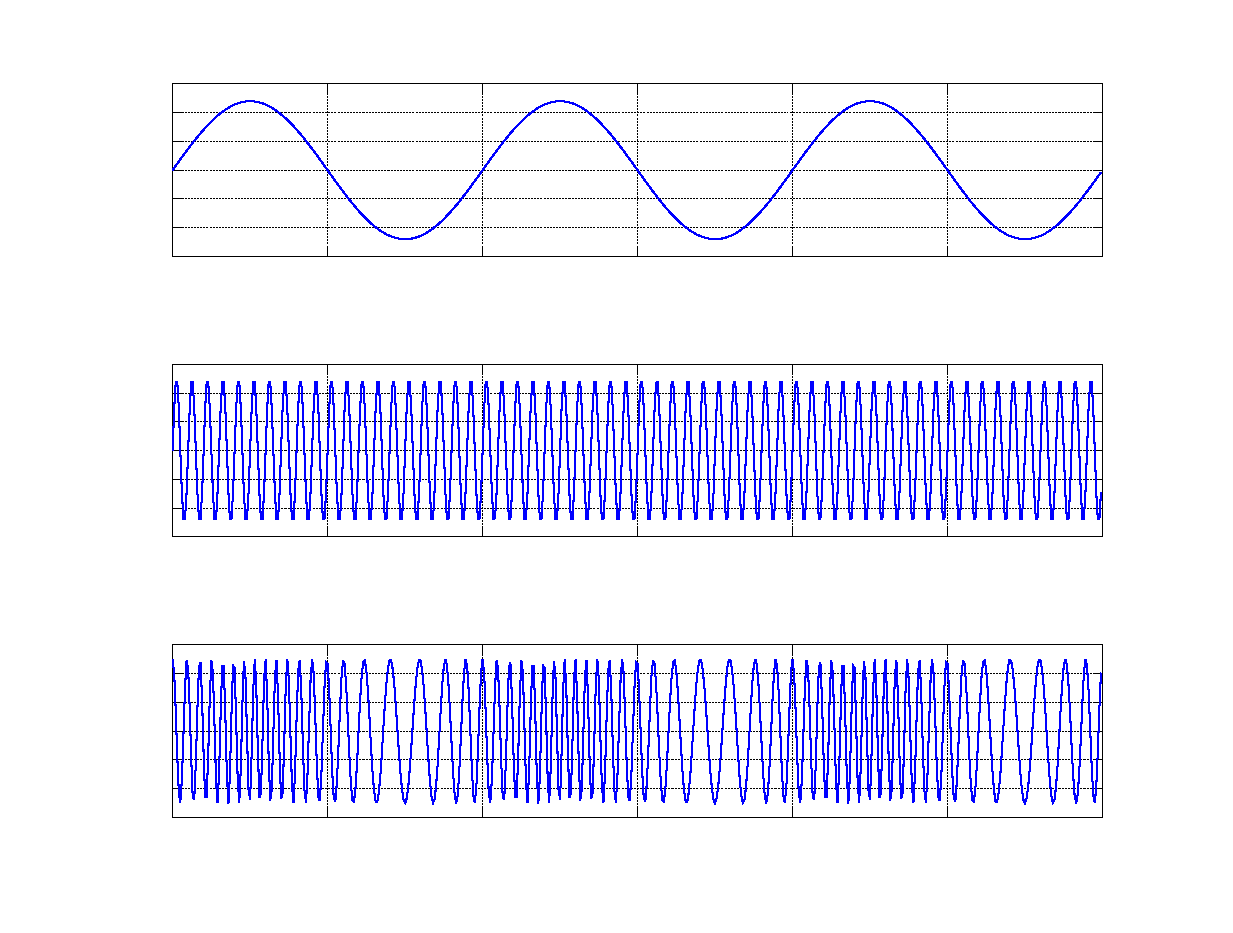
\includegraphics{fm}}%
    \gplfronttext
  \end{picture}%
\endgroup
$\end{large}}
  %% Creator: Matplotlib, PGF backend
%%
%% To include the figure in your LaTeX document, write
%%   \input{<filename>.pgf}
%%
%% Make sure the required packages are loaded in your preamble
%%   \usepackage{pgf}
%%
%% Figures using additional raster images can only be included by \input if
%% they are in the same directory as the main LaTeX file. For loading figures
%% from other directories you can use the `import` package
%%   \usepackage{import}
%% and then include the figures with
%%   \import{<path to file>}{<filename>.pgf}
%%
%% Matplotlib used the following preamble
%%   \usepackage[utf8x]{inputenc}
%%   \usepackage[T1]{fontenc}
%%
\begingroup%
\makeatletter%
\begin{pgfpicture}%
\pgfpathrectangle{\pgfpointorigin}{\pgfqpoint{5.396430in}{3.335177in}}%
\pgfusepath{use as bounding box, clip}%
\begin{pgfscope}%
\pgfsetbuttcap%
\pgfsetmiterjoin%
\definecolor{currentfill}{rgb}{1.000000,1.000000,1.000000}%
\pgfsetfillcolor{currentfill}%
\pgfsetlinewidth{0.000000pt}%
\definecolor{currentstroke}{rgb}{1.000000,1.000000,1.000000}%
\pgfsetstrokecolor{currentstroke}%
\pgfsetdash{}{0pt}%
\pgfpathmoveto{\pgfqpoint{0.000000in}{0.000000in}}%
\pgfpathlineto{\pgfqpoint{5.396430in}{0.000000in}}%
\pgfpathlineto{\pgfqpoint{5.396430in}{3.335177in}}%
\pgfpathlineto{\pgfqpoint{0.000000in}{3.335177in}}%
\pgfpathclose%
\pgfusepath{fill}%
\end{pgfscope}%
\begin{pgfscope}%
\pgfsetbuttcap%
\pgfsetmiterjoin%
\definecolor{currentfill}{rgb}{1.000000,1.000000,1.000000}%
\pgfsetfillcolor{currentfill}%
\pgfsetlinewidth{0.000000pt}%
\definecolor{currentstroke}{rgb}{0.000000,0.000000,0.000000}%
\pgfsetstrokecolor{currentstroke}%
\pgfsetstrokeopacity{0.000000}%
\pgfsetdash{}{0pt}%
\pgfpathmoveto{\pgfqpoint{0.557102in}{2.631761in}}%
\pgfpathlineto{\pgfqpoint{5.305874in}{2.631761in}}%
\pgfpathlineto{\pgfqpoint{5.305874in}{3.110198in}}%
\pgfpathlineto{\pgfqpoint{0.557102in}{3.110198in}}%
\pgfpathclose%
\pgfusepath{fill}%
\end{pgfscope}%
\begin{pgfscope}%
\pgfpathrectangle{\pgfqpoint{0.557102in}{2.631761in}}{\pgfqpoint{4.748773in}{0.478437in}} %
\pgfusepath{clip}%
\pgfsetbuttcap%
\pgfsetroundjoin%
\pgfsetlinewidth{0.501875pt}%
\definecolor{currentstroke}{rgb}{0.000000,0.000000,0.000000}%
\pgfsetstrokecolor{currentstroke}%
\pgfsetstrokeopacity{0.500000}%
\pgfsetdash{{2.200000pt}{2.200000pt}}{0.000000pt}%
\pgfpathmoveto{\pgfqpoint{0.557102in}{2.631761in}}%
\pgfpathlineto{\pgfqpoint{0.557102in}{3.110198in}}%
\pgfusepath{stroke}%
\end{pgfscope}%
\begin{pgfscope}%
\pgfsetbuttcap%
\pgfsetroundjoin%
\definecolor{currentfill}{rgb}{0.000000,0.000000,0.000000}%
\pgfsetfillcolor{currentfill}%
\pgfsetlinewidth{0.803000pt}%
\definecolor{currentstroke}{rgb}{0.000000,0.000000,0.000000}%
\pgfsetstrokecolor{currentstroke}%
\pgfsetdash{}{0pt}%
\pgfsys@defobject{currentmarker}{\pgfqpoint{0.000000in}{-0.048611in}}{\pgfqpoint{0.000000in}{0.000000in}}{%
\pgfpathmoveto{\pgfqpoint{0.000000in}{0.000000in}}%
\pgfpathlineto{\pgfqpoint{0.000000in}{-0.048611in}}%
\pgfusepath{stroke,fill}%
}%
\begin{pgfscope}%
\pgfsys@transformshift{0.557102in}{2.631761in}%
\pgfsys@useobject{currentmarker}{}%
\end{pgfscope}%
\end{pgfscope}%
\begin{pgfscope}%
\pgftext[x=0.557102in,y=2.534539in,,top]{\rmfamily\fontsize{8.000000}{9.600000}\selectfont \(\displaystyle 0.00\)}%
\end{pgfscope}%
\begin{pgfscope}%
\pgfpathrectangle{\pgfqpoint{0.557102in}{2.631761in}}{\pgfqpoint{4.748773in}{0.478437in}} %
\pgfusepath{clip}%
\pgfsetbuttcap%
\pgfsetroundjoin%
\pgfsetlinewidth{0.501875pt}%
\definecolor{currentstroke}{rgb}{0.000000,0.000000,0.000000}%
\pgfsetstrokecolor{currentstroke}%
\pgfsetstrokeopacity{0.500000}%
\pgfsetdash{{2.200000pt}{2.200000pt}}{0.000000pt}%
\pgfpathmoveto{\pgfqpoint{1.349885in}{2.631761in}}%
\pgfpathlineto{\pgfqpoint{1.349885in}{3.110198in}}%
\pgfusepath{stroke}%
\end{pgfscope}%
\begin{pgfscope}%
\pgfsetbuttcap%
\pgfsetroundjoin%
\definecolor{currentfill}{rgb}{0.000000,0.000000,0.000000}%
\pgfsetfillcolor{currentfill}%
\pgfsetlinewidth{0.803000pt}%
\definecolor{currentstroke}{rgb}{0.000000,0.000000,0.000000}%
\pgfsetstrokecolor{currentstroke}%
\pgfsetdash{}{0pt}%
\pgfsys@defobject{currentmarker}{\pgfqpoint{0.000000in}{-0.048611in}}{\pgfqpoint{0.000000in}{0.000000in}}{%
\pgfpathmoveto{\pgfqpoint{0.000000in}{0.000000in}}%
\pgfpathlineto{\pgfqpoint{0.000000in}{-0.048611in}}%
\pgfusepath{stroke,fill}%
}%
\begin{pgfscope}%
\pgfsys@transformshift{1.349885in}{2.631761in}%
\pgfsys@useobject{currentmarker}{}%
\end{pgfscope}%
\end{pgfscope}%
\begin{pgfscope}%
\pgftext[x=1.349885in,y=2.534539in,,top]{\rmfamily\fontsize{8.000000}{9.600000}\selectfont \(\displaystyle 0.01\)}%
\end{pgfscope}%
\begin{pgfscope}%
\pgfpathrectangle{\pgfqpoint{0.557102in}{2.631761in}}{\pgfqpoint{4.748773in}{0.478437in}} %
\pgfusepath{clip}%
\pgfsetbuttcap%
\pgfsetroundjoin%
\pgfsetlinewidth{0.501875pt}%
\definecolor{currentstroke}{rgb}{0.000000,0.000000,0.000000}%
\pgfsetstrokecolor{currentstroke}%
\pgfsetstrokeopacity{0.500000}%
\pgfsetdash{{2.200000pt}{2.200000pt}}{0.000000pt}%
\pgfpathmoveto{\pgfqpoint{2.142669in}{2.631761in}}%
\pgfpathlineto{\pgfqpoint{2.142669in}{3.110198in}}%
\pgfusepath{stroke}%
\end{pgfscope}%
\begin{pgfscope}%
\pgfsetbuttcap%
\pgfsetroundjoin%
\definecolor{currentfill}{rgb}{0.000000,0.000000,0.000000}%
\pgfsetfillcolor{currentfill}%
\pgfsetlinewidth{0.803000pt}%
\definecolor{currentstroke}{rgb}{0.000000,0.000000,0.000000}%
\pgfsetstrokecolor{currentstroke}%
\pgfsetdash{}{0pt}%
\pgfsys@defobject{currentmarker}{\pgfqpoint{0.000000in}{-0.048611in}}{\pgfqpoint{0.000000in}{0.000000in}}{%
\pgfpathmoveto{\pgfqpoint{0.000000in}{0.000000in}}%
\pgfpathlineto{\pgfqpoint{0.000000in}{-0.048611in}}%
\pgfusepath{stroke,fill}%
}%
\begin{pgfscope}%
\pgfsys@transformshift{2.142669in}{2.631761in}%
\pgfsys@useobject{currentmarker}{}%
\end{pgfscope}%
\end{pgfscope}%
\begin{pgfscope}%
\pgftext[x=2.142669in,y=2.534539in,,top]{\rmfamily\fontsize{8.000000}{9.600000}\selectfont \(\displaystyle 0.02\)}%
\end{pgfscope}%
\begin{pgfscope}%
\pgfpathrectangle{\pgfqpoint{0.557102in}{2.631761in}}{\pgfqpoint{4.748773in}{0.478437in}} %
\pgfusepath{clip}%
\pgfsetbuttcap%
\pgfsetroundjoin%
\pgfsetlinewidth{0.501875pt}%
\definecolor{currentstroke}{rgb}{0.000000,0.000000,0.000000}%
\pgfsetstrokecolor{currentstroke}%
\pgfsetstrokeopacity{0.500000}%
\pgfsetdash{{2.200000pt}{2.200000pt}}{0.000000pt}%
\pgfpathmoveto{\pgfqpoint{2.935452in}{2.631761in}}%
\pgfpathlineto{\pgfqpoint{2.935452in}{3.110198in}}%
\pgfusepath{stroke}%
\end{pgfscope}%
\begin{pgfscope}%
\pgfsetbuttcap%
\pgfsetroundjoin%
\definecolor{currentfill}{rgb}{0.000000,0.000000,0.000000}%
\pgfsetfillcolor{currentfill}%
\pgfsetlinewidth{0.803000pt}%
\definecolor{currentstroke}{rgb}{0.000000,0.000000,0.000000}%
\pgfsetstrokecolor{currentstroke}%
\pgfsetdash{}{0pt}%
\pgfsys@defobject{currentmarker}{\pgfqpoint{0.000000in}{-0.048611in}}{\pgfqpoint{0.000000in}{0.000000in}}{%
\pgfpathmoveto{\pgfqpoint{0.000000in}{0.000000in}}%
\pgfpathlineto{\pgfqpoint{0.000000in}{-0.048611in}}%
\pgfusepath{stroke,fill}%
}%
\begin{pgfscope}%
\pgfsys@transformshift{2.935452in}{2.631761in}%
\pgfsys@useobject{currentmarker}{}%
\end{pgfscope}%
\end{pgfscope}%
\begin{pgfscope}%
\pgftext[x=2.935452in,y=2.534539in,,top]{\rmfamily\fontsize{8.000000}{9.600000}\selectfont \(\displaystyle 0.03\)}%
\end{pgfscope}%
\begin{pgfscope}%
\pgfpathrectangle{\pgfqpoint{0.557102in}{2.631761in}}{\pgfqpoint{4.748773in}{0.478437in}} %
\pgfusepath{clip}%
\pgfsetbuttcap%
\pgfsetroundjoin%
\pgfsetlinewidth{0.501875pt}%
\definecolor{currentstroke}{rgb}{0.000000,0.000000,0.000000}%
\pgfsetstrokecolor{currentstroke}%
\pgfsetstrokeopacity{0.500000}%
\pgfsetdash{{2.200000pt}{2.200000pt}}{0.000000pt}%
\pgfpathmoveto{\pgfqpoint{3.728235in}{2.631761in}}%
\pgfpathlineto{\pgfqpoint{3.728235in}{3.110198in}}%
\pgfusepath{stroke}%
\end{pgfscope}%
\begin{pgfscope}%
\pgfsetbuttcap%
\pgfsetroundjoin%
\definecolor{currentfill}{rgb}{0.000000,0.000000,0.000000}%
\pgfsetfillcolor{currentfill}%
\pgfsetlinewidth{0.803000pt}%
\definecolor{currentstroke}{rgb}{0.000000,0.000000,0.000000}%
\pgfsetstrokecolor{currentstroke}%
\pgfsetdash{}{0pt}%
\pgfsys@defobject{currentmarker}{\pgfqpoint{0.000000in}{-0.048611in}}{\pgfqpoint{0.000000in}{0.000000in}}{%
\pgfpathmoveto{\pgfqpoint{0.000000in}{0.000000in}}%
\pgfpathlineto{\pgfqpoint{0.000000in}{-0.048611in}}%
\pgfusepath{stroke,fill}%
}%
\begin{pgfscope}%
\pgfsys@transformshift{3.728235in}{2.631761in}%
\pgfsys@useobject{currentmarker}{}%
\end{pgfscope}%
\end{pgfscope}%
\begin{pgfscope}%
\pgftext[x=3.728235in,y=2.534539in,,top]{\rmfamily\fontsize{8.000000}{9.600000}\selectfont \(\displaystyle 0.04\)}%
\end{pgfscope}%
\begin{pgfscope}%
\pgfpathrectangle{\pgfqpoint{0.557102in}{2.631761in}}{\pgfqpoint{4.748773in}{0.478437in}} %
\pgfusepath{clip}%
\pgfsetbuttcap%
\pgfsetroundjoin%
\pgfsetlinewidth{0.501875pt}%
\definecolor{currentstroke}{rgb}{0.000000,0.000000,0.000000}%
\pgfsetstrokecolor{currentstroke}%
\pgfsetstrokeopacity{0.500000}%
\pgfsetdash{{2.200000pt}{2.200000pt}}{0.000000pt}%
\pgfpathmoveto{\pgfqpoint{4.521019in}{2.631761in}}%
\pgfpathlineto{\pgfqpoint{4.521019in}{3.110198in}}%
\pgfusepath{stroke}%
\end{pgfscope}%
\begin{pgfscope}%
\pgfsetbuttcap%
\pgfsetroundjoin%
\definecolor{currentfill}{rgb}{0.000000,0.000000,0.000000}%
\pgfsetfillcolor{currentfill}%
\pgfsetlinewidth{0.803000pt}%
\definecolor{currentstroke}{rgb}{0.000000,0.000000,0.000000}%
\pgfsetstrokecolor{currentstroke}%
\pgfsetdash{}{0pt}%
\pgfsys@defobject{currentmarker}{\pgfqpoint{0.000000in}{-0.048611in}}{\pgfqpoint{0.000000in}{0.000000in}}{%
\pgfpathmoveto{\pgfqpoint{0.000000in}{0.000000in}}%
\pgfpathlineto{\pgfqpoint{0.000000in}{-0.048611in}}%
\pgfusepath{stroke,fill}%
}%
\begin{pgfscope}%
\pgfsys@transformshift{4.521019in}{2.631761in}%
\pgfsys@useobject{currentmarker}{}%
\end{pgfscope}%
\end{pgfscope}%
\begin{pgfscope}%
\pgftext[x=4.521019in,y=2.534539in,,top]{\rmfamily\fontsize{8.000000}{9.600000}\selectfont \(\displaystyle 0.05\)}%
\end{pgfscope}%
\begin{pgfscope}%
\pgftext[x=2.931488in,y=2.380859in,,top]{\rmfamily\fontsize{10.000000}{12.000000}\selectfont \(\displaystyle t/s\)}%
\end{pgfscope}%
\begin{pgfscope}%
\pgfpathrectangle{\pgfqpoint{0.557102in}{2.631761in}}{\pgfqpoint{4.748773in}{0.478437in}} %
\pgfusepath{clip}%
\pgfsetbuttcap%
\pgfsetroundjoin%
\pgfsetlinewidth{0.501875pt}%
\definecolor{currentstroke}{rgb}{0.000000,0.000000,0.000000}%
\pgfsetstrokecolor{currentstroke}%
\pgfsetstrokeopacity{0.500000}%
\pgfsetdash{{2.200000pt}{2.200000pt}}{0.000000pt}%
\pgfpathmoveto{\pgfqpoint{0.557102in}{2.711500in}}%
\pgfpathlineto{\pgfqpoint{5.305874in}{2.711500in}}%
\pgfusepath{stroke}%
\end{pgfscope}%
\begin{pgfscope}%
\pgfsetbuttcap%
\pgfsetroundjoin%
\definecolor{currentfill}{rgb}{0.000000,0.000000,0.000000}%
\pgfsetfillcolor{currentfill}%
\pgfsetlinewidth{0.803000pt}%
\definecolor{currentstroke}{rgb}{0.000000,0.000000,0.000000}%
\pgfsetstrokecolor{currentstroke}%
\pgfsetdash{}{0pt}%
\pgfsys@defobject{currentmarker}{\pgfqpoint{-0.048611in}{0.000000in}}{\pgfqpoint{0.000000in}{0.000000in}}{%
\pgfpathmoveto{\pgfqpoint{0.000000in}{0.000000in}}%
\pgfpathlineto{\pgfqpoint{-0.048611in}{0.000000in}}%
\pgfusepath{stroke,fill}%
}%
\begin{pgfscope}%
\pgfsys@transformshift{0.557102in}{2.711500in}%
\pgfsys@useobject{currentmarker}{}%
\end{pgfscope}%
\end{pgfscope}%
\begin{pgfscope}%
\pgftext[x=0.250000in,y=2.673238in,left,base]{\rmfamily\fontsize{8.000000}{9.600000}\selectfont \(\displaystyle -10\)}%
\end{pgfscope}%
\begin{pgfscope}%
\pgfpathrectangle{\pgfqpoint{0.557102in}{2.631761in}}{\pgfqpoint{4.748773in}{0.478437in}} %
\pgfusepath{clip}%
\pgfsetbuttcap%
\pgfsetroundjoin%
\pgfsetlinewidth{0.501875pt}%
\definecolor{currentstroke}{rgb}{0.000000,0.000000,0.000000}%
\pgfsetstrokecolor{currentstroke}%
\pgfsetstrokeopacity{0.500000}%
\pgfsetdash{{2.200000pt}{2.200000pt}}{0.000000pt}%
\pgfpathmoveto{\pgfqpoint{0.557102in}{2.870980in}}%
\pgfpathlineto{\pgfqpoint{5.305874in}{2.870980in}}%
\pgfusepath{stroke}%
\end{pgfscope}%
\begin{pgfscope}%
\pgfsetbuttcap%
\pgfsetroundjoin%
\definecolor{currentfill}{rgb}{0.000000,0.000000,0.000000}%
\pgfsetfillcolor{currentfill}%
\pgfsetlinewidth{0.803000pt}%
\definecolor{currentstroke}{rgb}{0.000000,0.000000,0.000000}%
\pgfsetstrokecolor{currentstroke}%
\pgfsetdash{}{0pt}%
\pgfsys@defobject{currentmarker}{\pgfqpoint{-0.048611in}{0.000000in}}{\pgfqpoint{0.000000in}{0.000000in}}{%
\pgfpathmoveto{\pgfqpoint{0.000000in}{0.000000in}}%
\pgfpathlineto{\pgfqpoint{-0.048611in}{0.000000in}}%
\pgfusepath{stroke,fill}%
}%
\begin{pgfscope}%
\pgfsys@transformshift{0.557102in}{2.870980in}%
\pgfsys@useobject{currentmarker}{}%
\end{pgfscope}%
\end{pgfscope}%
\begin{pgfscope}%
\pgftext[x=0.400851in,y=2.832717in,left,base]{\rmfamily\fontsize{8.000000}{9.600000}\selectfont \(\displaystyle 0\)}%
\end{pgfscope}%
\begin{pgfscope}%
\pgfpathrectangle{\pgfqpoint{0.557102in}{2.631761in}}{\pgfqpoint{4.748773in}{0.478437in}} %
\pgfusepath{clip}%
\pgfsetbuttcap%
\pgfsetroundjoin%
\pgfsetlinewidth{0.501875pt}%
\definecolor{currentstroke}{rgb}{0.000000,0.000000,0.000000}%
\pgfsetstrokecolor{currentstroke}%
\pgfsetstrokeopacity{0.500000}%
\pgfsetdash{{2.200000pt}{2.200000pt}}{0.000000pt}%
\pgfpathmoveto{\pgfqpoint{0.557102in}{3.030459in}}%
\pgfpathlineto{\pgfqpoint{5.305874in}{3.030459in}}%
\pgfusepath{stroke}%
\end{pgfscope}%
\begin{pgfscope}%
\pgfsetbuttcap%
\pgfsetroundjoin%
\definecolor{currentfill}{rgb}{0.000000,0.000000,0.000000}%
\pgfsetfillcolor{currentfill}%
\pgfsetlinewidth{0.803000pt}%
\definecolor{currentstroke}{rgb}{0.000000,0.000000,0.000000}%
\pgfsetstrokecolor{currentstroke}%
\pgfsetdash{}{0pt}%
\pgfsys@defobject{currentmarker}{\pgfqpoint{-0.048611in}{0.000000in}}{\pgfqpoint{0.000000in}{0.000000in}}{%
\pgfpathmoveto{\pgfqpoint{0.000000in}{0.000000in}}%
\pgfpathlineto{\pgfqpoint{-0.048611in}{0.000000in}}%
\pgfusepath{stroke,fill}%
}%
\begin{pgfscope}%
\pgfsys@transformshift{0.557102in}{3.030459in}%
\pgfsys@useobject{currentmarker}{}%
\end{pgfscope}%
\end{pgfscope}%
\begin{pgfscope}%
\pgftext[x=0.341822in,y=2.992196in,left,base]{\rmfamily\fontsize{8.000000}{9.600000}\selectfont \(\displaystyle 10\)}%
\end{pgfscope}%
\begin{pgfscope}%
\pgftext[x=0.194444in,y=2.870980in,,bottom,rotate=90.000000]{\rmfamily\fontsize{10.000000}{12.000000}\selectfont \(\displaystyle u_{m}/V\)}%
\end{pgfscope}%
\begin{pgfscope}%
\pgfpathrectangle{\pgfqpoint{0.557102in}{2.631761in}}{\pgfqpoint{4.748773in}{0.478437in}} %
\pgfusepath{clip}%
\pgfsetrectcap%
\pgfsetroundjoin%
\pgfsetlinewidth{0.752812pt}%
\definecolor{currentstroke}{rgb}{0.121569,0.466667,0.705882}%
\pgfsetstrokecolor{currentstroke}%
\pgfsetdash{}{0pt}%
\pgfpathmoveto{\pgfqpoint{0.557102in}{2.870980in}}%
\pgfpathlineto{\pgfqpoint{0.644308in}{2.935805in}}%
\pgfpathlineto{\pgfqpoint{0.691875in}{2.968397in}}%
\pgfpathlineto{\pgfqpoint{0.731514in}{2.992967in}}%
\pgfpathlineto{\pgfqpoint{0.763225in}{3.010486in}}%
\pgfpathlineto{\pgfqpoint{0.794937in}{3.025805in}}%
\pgfpathlineto{\pgfqpoint{0.826648in}{3.038683in}}%
\pgfpathlineto{\pgfqpoint{0.858360in}{3.048915in}}%
\pgfpathlineto{\pgfqpoint{0.890071in}{3.056342in}}%
\pgfpathlineto{\pgfqpoint{0.921782in}{3.060845in}}%
\pgfpathlineto{\pgfqpoint{0.945566in}{3.062260in}}%
\pgfpathlineto{\pgfqpoint{0.969349in}{3.061977in}}%
\pgfpathlineto{\pgfqpoint{0.993133in}{3.059998in}}%
\pgfpathlineto{\pgfqpoint{1.024844in}{3.054756in}}%
\pgfpathlineto{\pgfqpoint{1.056555in}{3.046615in}}%
\pgfpathlineto{\pgfqpoint{1.088267in}{3.035704in}}%
\pgfpathlineto{\pgfqpoint{1.119978in}{3.022195in}}%
\pgfpathlineto{\pgfqpoint{1.151689in}{3.006302in}}%
\pgfpathlineto{\pgfqpoint{1.191329in}{2.983467in}}%
\pgfpathlineto{\pgfqpoint{1.230968in}{2.957862in}}%
\pgfpathlineto{\pgfqpoint{1.278535in}{2.924371in}}%
\pgfpathlineto{\pgfqpoint{1.349885in}{2.870980in}}%
\pgfpathlineto{\pgfqpoint{1.437091in}{2.806154in}}%
\pgfpathlineto{\pgfqpoint{1.484658in}{2.773562in}}%
\pgfpathlineto{\pgfqpoint{1.524298in}{2.748993in}}%
\pgfpathlineto{\pgfqpoint{1.556009in}{2.731473in}}%
\pgfpathlineto{\pgfqpoint{1.587720in}{2.716154in}}%
\pgfpathlineto{\pgfqpoint{1.619432in}{2.703276in}}%
\pgfpathlineto{\pgfqpoint{1.651143in}{2.693044in}}%
\pgfpathlineto{\pgfqpoint{1.682854in}{2.685617in}}%
\pgfpathlineto{\pgfqpoint{1.714566in}{2.681114in}}%
\pgfpathlineto{\pgfqpoint{1.738349in}{2.679699in}}%
\pgfpathlineto{\pgfqpoint{1.762133in}{2.679982in}}%
\pgfpathlineto{\pgfqpoint{1.785916in}{2.681961in}}%
\pgfpathlineto{\pgfqpoint{1.817627in}{2.687203in}}%
\pgfpathlineto{\pgfqpoint{1.849339in}{2.695344in}}%
\pgfpathlineto{\pgfqpoint{1.881050in}{2.706255in}}%
\pgfpathlineto{\pgfqpoint{1.912761in}{2.719764in}}%
\pgfpathlineto{\pgfqpoint{1.944473in}{2.735657in}}%
\pgfpathlineto{\pgfqpoint{1.984112in}{2.758492in}}%
\pgfpathlineto{\pgfqpoint{2.023751in}{2.784097in}}%
\pgfpathlineto{\pgfqpoint{2.071318in}{2.817588in}}%
\pgfpathlineto{\pgfqpoint{2.142669in}{2.870980in}}%
\pgfpathlineto{\pgfqpoint{2.229875in}{2.935805in}}%
\pgfpathlineto{\pgfqpoint{2.277442in}{2.968397in}}%
\pgfpathlineto{\pgfqpoint{2.317081in}{2.992967in}}%
\pgfpathlineto{\pgfqpoint{2.348792in}{3.010486in}}%
\pgfpathlineto{\pgfqpoint{2.380504in}{3.025805in}}%
\pgfpathlineto{\pgfqpoint{2.412215in}{3.038683in}}%
\pgfpathlineto{\pgfqpoint{2.443926in}{3.048915in}}%
\pgfpathlineto{\pgfqpoint{2.475638in}{3.056342in}}%
\pgfpathlineto{\pgfqpoint{2.507349in}{3.060845in}}%
\pgfpathlineto{\pgfqpoint{2.531133in}{3.062260in}}%
\pgfpathlineto{\pgfqpoint{2.554916in}{3.061977in}}%
\pgfpathlineto{\pgfqpoint{2.578700in}{3.059998in}}%
\pgfpathlineto{\pgfqpoint{2.610411in}{3.054756in}}%
\pgfpathlineto{\pgfqpoint{2.642122in}{3.046615in}}%
\pgfpathlineto{\pgfqpoint{2.673834in}{3.035704in}}%
\pgfpathlineto{\pgfqpoint{2.705545in}{3.022195in}}%
\pgfpathlineto{\pgfqpoint{2.737256in}{3.006302in}}%
\pgfpathlineto{\pgfqpoint{2.776895in}{2.983467in}}%
\pgfpathlineto{\pgfqpoint{2.816535in}{2.957862in}}%
\pgfpathlineto{\pgfqpoint{2.864102in}{2.924371in}}%
\pgfpathlineto{\pgfqpoint{2.935452in}{2.870980in}}%
\pgfpathlineto{\pgfqpoint{3.022658in}{2.806154in}}%
\pgfpathlineto{\pgfqpoint{3.070225in}{2.773562in}}%
\pgfpathlineto{\pgfqpoint{3.109864in}{2.748993in}}%
\pgfpathlineto{\pgfqpoint{3.141576in}{2.731473in}}%
\pgfpathlineto{\pgfqpoint{3.173287in}{2.716154in}}%
\pgfpathlineto{\pgfqpoint{3.204998in}{2.703276in}}%
\pgfpathlineto{\pgfqpoint{3.236710in}{2.693044in}}%
\pgfpathlineto{\pgfqpoint{3.268421in}{2.685617in}}%
\pgfpathlineto{\pgfqpoint{3.300132in}{2.681114in}}%
\pgfpathlineto{\pgfqpoint{3.323916in}{2.679699in}}%
\pgfpathlineto{\pgfqpoint{3.347699in}{2.679982in}}%
\pgfpathlineto{\pgfqpoint{3.371483in}{2.681961in}}%
\pgfpathlineto{\pgfqpoint{3.403194in}{2.687203in}}%
\pgfpathlineto{\pgfqpoint{3.434906in}{2.695344in}}%
\pgfpathlineto{\pgfqpoint{3.466617in}{2.706255in}}%
\pgfpathlineto{\pgfqpoint{3.498328in}{2.719764in}}%
\pgfpathlineto{\pgfqpoint{3.530040in}{2.735657in}}%
\pgfpathlineto{\pgfqpoint{3.569679in}{2.758492in}}%
\pgfpathlineto{\pgfqpoint{3.609318in}{2.784097in}}%
\pgfpathlineto{\pgfqpoint{3.656885in}{2.817588in}}%
\pgfpathlineto{\pgfqpoint{3.728235in}{2.870980in}}%
\pgfpathlineto{\pgfqpoint{3.815442in}{2.935805in}}%
\pgfpathlineto{\pgfqpoint{3.863009in}{2.968397in}}%
\pgfpathlineto{\pgfqpoint{3.902648in}{2.992967in}}%
\pgfpathlineto{\pgfqpoint{3.934359in}{3.010486in}}%
\pgfpathlineto{\pgfqpoint{3.966071in}{3.025805in}}%
\pgfpathlineto{\pgfqpoint{3.997782in}{3.038683in}}%
\pgfpathlineto{\pgfqpoint{4.029493in}{3.048915in}}%
\pgfpathlineto{\pgfqpoint{4.061205in}{3.056342in}}%
\pgfpathlineto{\pgfqpoint{4.092916in}{3.060845in}}%
\pgfpathlineto{\pgfqpoint{4.116699in}{3.062260in}}%
\pgfpathlineto{\pgfqpoint{4.140483in}{3.061977in}}%
\pgfpathlineto{\pgfqpoint{4.164266in}{3.059998in}}%
\pgfpathlineto{\pgfqpoint{4.195978in}{3.054756in}}%
\pgfpathlineto{\pgfqpoint{4.227689in}{3.046615in}}%
\pgfpathlineto{\pgfqpoint{4.259400in}{3.035704in}}%
\pgfpathlineto{\pgfqpoint{4.291112in}{3.022195in}}%
\pgfpathlineto{\pgfqpoint{4.322823in}{3.006302in}}%
\pgfpathlineto{\pgfqpoint{4.362462in}{2.983467in}}%
\pgfpathlineto{\pgfqpoint{4.402101in}{2.957862in}}%
\pgfpathlineto{\pgfqpoint{4.449668in}{2.924371in}}%
\pgfpathlineto{\pgfqpoint{4.521019in}{2.870980in}}%
\pgfpathlineto{\pgfqpoint{4.608225in}{2.806154in}}%
\pgfpathlineto{\pgfqpoint{4.655792in}{2.773562in}}%
\pgfpathlineto{\pgfqpoint{4.695431in}{2.748993in}}%
\pgfpathlineto{\pgfqpoint{4.727143in}{2.731473in}}%
\pgfpathlineto{\pgfqpoint{4.758854in}{2.716154in}}%
\pgfpathlineto{\pgfqpoint{4.790565in}{2.703276in}}%
\pgfpathlineto{\pgfqpoint{4.822277in}{2.693044in}}%
\pgfpathlineto{\pgfqpoint{4.853988in}{2.685617in}}%
\pgfpathlineto{\pgfqpoint{4.885699in}{2.681114in}}%
\pgfpathlineto{\pgfqpoint{4.909483in}{2.679699in}}%
\pgfpathlineto{\pgfqpoint{4.933266in}{2.679982in}}%
\pgfpathlineto{\pgfqpoint{4.957050in}{2.681961in}}%
\pgfpathlineto{\pgfqpoint{4.988761in}{2.687203in}}%
\pgfpathlineto{\pgfqpoint{5.020472in}{2.695344in}}%
\pgfpathlineto{\pgfqpoint{5.052184in}{2.706255in}}%
\pgfpathlineto{\pgfqpoint{5.083895in}{2.719764in}}%
\pgfpathlineto{\pgfqpoint{5.115606in}{2.735657in}}%
\pgfpathlineto{\pgfqpoint{5.155246in}{2.758492in}}%
\pgfpathlineto{\pgfqpoint{5.194885in}{2.784097in}}%
\pgfpathlineto{\pgfqpoint{5.242452in}{2.817588in}}%
\pgfpathlineto{\pgfqpoint{5.305874in}{2.864968in}}%
\pgfpathlineto{\pgfqpoint{5.305874in}{2.864968in}}%
\pgfusepath{stroke}%
\end{pgfscope}%
\begin{pgfscope}%
\pgfsetrectcap%
\pgfsetmiterjoin%
\pgfsetlinewidth{0.501875pt}%
\definecolor{currentstroke}{rgb}{0.000000,0.000000,0.000000}%
\pgfsetstrokecolor{currentstroke}%
\pgfsetdash{}{0pt}%
\pgfpathmoveto{\pgfqpoint{0.557102in}{2.631761in}}%
\pgfpathlineto{\pgfqpoint{0.557102in}{3.110198in}}%
\pgfusepath{stroke}%
\end{pgfscope}%
\begin{pgfscope}%
\pgfsetrectcap%
\pgfsetmiterjoin%
\pgfsetlinewidth{0.501875pt}%
\definecolor{currentstroke}{rgb}{0.000000,0.000000,0.000000}%
\pgfsetstrokecolor{currentstroke}%
\pgfsetdash{}{0pt}%
\pgfpathmoveto{\pgfqpoint{5.305874in}{2.631761in}}%
\pgfpathlineto{\pgfqpoint{5.305874in}{3.110198in}}%
\pgfusepath{stroke}%
\end{pgfscope}%
\begin{pgfscope}%
\pgfsetrectcap%
\pgfsetmiterjoin%
\pgfsetlinewidth{0.501875pt}%
\definecolor{currentstroke}{rgb}{0.000000,0.000000,0.000000}%
\pgfsetstrokecolor{currentstroke}%
\pgfsetdash{}{0pt}%
\pgfpathmoveto{\pgfqpoint{0.557102in}{2.631761in}}%
\pgfpathlineto{\pgfqpoint{5.305874in}{2.631761in}}%
\pgfusepath{stroke}%
\end{pgfscope}%
\begin{pgfscope}%
\pgfsetrectcap%
\pgfsetmiterjoin%
\pgfsetlinewidth{0.501875pt}%
\definecolor{currentstroke}{rgb}{0.000000,0.000000,0.000000}%
\pgfsetstrokecolor{currentstroke}%
\pgfsetdash{}{0pt}%
\pgfpathmoveto{\pgfqpoint{0.557102in}{3.110198in}}%
\pgfpathlineto{\pgfqpoint{5.305874in}{3.110198in}}%
\pgfusepath{stroke}%
\end{pgfscope}%
\begin{pgfscope}%
\pgftext[x=2.931488in,y=3.193531in,,base]{\rmfamily\fontsize{9.000000}{10.800000}\selectfont Nachrichtensignal}%
\end{pgfscope}%
\begin{pgfscope}%
\pgfsetbuttcap%
\pgfsetmiterjoin%
\definecolor{currentfill}{rgb}{1.000000,1.000000,1.000000}%
\pgfsetfillcolor{currentfill}%
\pgfsetlinewidth{0.000000pt}%
\definecolor{currentstroke}{rgb}{0.000000,0.000000,0.000000}%
\pgfsetstrokecolor{currentstroke}%
\pgfsetstrokeopacity{0.000000}%
\pgfsetdash{}{0pt}%
\pgfpathmoveto{\pgfqpoint{0.557102in}{1.538554in}}%
\pgfpathlineto{\pgfqpoint{5.305874in}{1.538554in}}%
\pgfpathlineto{\pgfqpoint{5.305874in}{2.016991in}}%
\pgfpathlineto{\pgfqpoint{0.557102in}{2.016991in}}%
\pgfpathclose%
\pgfusepath{fill}%
\end{pgfscope}%
\begin{pgfscope}%
\pgfpathrectangle{\pgfqpoint{0.557102in}{1.538554in}}{\pgfqpoint{4.748773in}{0.478437in}} %
\pgfusepath{clip}%
\pgfsetbuttcap%
\pgfsetroundjoin%
\pgfsetlinewidth{0.501875pt}%
\definecolor{currentstroke}{rgb}{0.000000,0.000000,0.000000}%
\pgfsetstrokecolor{currentstroke}%
\pgfsetstrokeopacity{0.500000}%
\pgfsetdash{{2.200000pt}{2.200000pt}}{0.000000pt}%
\pgfpathmoveto{\pgfqpoint{0.557102in}{1.538554in}}%
\pgfpathlineto{\pgfqpoint{0.557102in}{2.016991in}}%
\pgfusepath{stroke}%
\end{pgfscope}%
\begin{pgfscope}%
\pgfsetbuttcap%
\pgfsetroundjoin%
\definecolor{currentfill}{rgb}{0.000000,0.000000,0.000000}%
\pgfsetfillcolor{currentfill}%
\pgfsetlinewidth{0.803000pt}%
\definecolor{currentstroke}{rgb}{0.000000,0.000000,0.000000}%
\pgfsetstrokecolor{currentstroke}%
\pgfsetdash{}{0pt}%
\pgfsys@defobject{currentmarker}{\pgfqpoint{0.000000in}{-0.048611in}}{\pgfqpoint{0.000000in}{0.000000in}}{%
\pgfpathmoveto{\pgfqpoint{0.000000in}{0.000000in}}%
\pgfpathlineto{\pgfqpoint{0.000000in}{-0.048611in}}%
\pgfusepath{stroke,fill}%
}%
\begin{pgfscope}%
\pgfsys@transformshift{0.557102in}{1.538554in}%
\pgfsys@useobject{currentmarker}{}%
\end{pgfscope}%
\end{pgfscope}%
\begin{pgfscope}%
\pgftext[x=0.557102in,y=1.441332in,,top]{\rmfamily\fontsize{8.000000}{9.600000}\selectfont \(\displaystyle 0.00\)}%
\end{pgfscope}%
\begin{pgfscope}%
\pgfpathrectangle{\pgfqpoint{0.557102in}{1.538554in}}{\pgfqpoint{4.748773in}{0.478437in}} %
\pgfusepath{clip}%
\pgfsetbuttcap%
\pgfsetroundjoin%
\pgfsetlinewidth{0.501875pt}%
\definecolor{currentstroke}{rgb}{0.000000,0.000000,0.000000}%
\pgfsetstrokecolor{currentstroke}%
\pgfsetstrokeopacity{0.500000}%
\pgfsetdash{{2.200000pt}{2.200000pt}}{0.000000pt}%
\pgfpathmoveto{\pgfqpoint{1.349885in}{1.538554in}}%
\pgfpathlineto{\pgfqpoint{1.349885in}{2.016991in}}%
\pgfusepath{stroke}%
\end{pgfscope}%
\begin{pgfscope}%
\pgfsetbuttcap%
\pgfsetroundjoin%
\definecolor{currentfill}{rgb}{0.000000,0.000000,0.000000}%
\pgfsetfillcolor{currentfill}%
\pgfsetlinewidth{0.803000pt}%
\definecolor{currentstroke}{rgb}{0.000000,0.000000,0.000000}%
\pgfsetstrokecolor{currentstroke}%
\pgfsetdash{}{0pt}%
\pgfsys@defobject{currentmarker}{\pgfqpoint{0.000000in}{-0.048611in}}{\pgfqpoint{0.000000in}{0.000000in}}{%
\pgfpathmoveto{\pgfqpoint{0.000000in}{0.000000in}}%
\pgfpathlineto{\pgfqpoint{0.000000in}{-0.048611in}}%
\pgfusepath{stroke,fill}%
}%
\begin{pgfscope}%
\pgfsys@transformshift{1.349885in}{1.538554in}%
\pgfsys@useobject{currentmarker}{}%
\end{pgfscope}%
\end{pgfscope}%
\begin{pgfscope}%
\pgftext[x=1.349885in,y=1.441332in,,top]{\rmfamily\fontsize{8.000000}{9.600000}\selectfont \(\displaystyle 0.01\)}%
\end{pgfscope}%
\begin{pgfscope}%
\pgfpathrectangle{\pgfqpoint{0.557102in}{1.538554in}}{\pgfqpoint{4.748773in}{0.478437in}} %
\pgfusepath{clip}%
\pgfsetbuttcap%
\pgfsetroundjoin%
\pgfsetlinewidth{0.501875pt}%
\definecolor{currentstroke}{rgb}{0.000000,0.000000,0.000000}%
\pgfsetstrokecolor{currentstroke}%
\pgfsetstrokeopacity{0.500000}%
\pgfsetdash{{2.200000pt}{2.200000pt}}{0.000000pt}%
\pgfpathmoveto{\pgfqpoint{2.142669in}{1.538554in}}%
\pgfpathlineto{\pgfqpoint{2.142669in}{2.016991in}}%
\pgfusepath{stroke}%
\end{pgfscope}%
\begin{pgfscope}%
\pgfsetbuttcap%
\pgfsetroundjoin%
\definecolor{currentfill}{rgb}{0.000000,0.000000,0.000000}%
\pgfsetfillcolor{currentfill}%
\pgfsetlinewidth{0.803000pt}%
\definecolor{currentstroke}{rgb}{0.000000,0.000000,0.000000}%
\pgfsetstrokecolor{currentstroke}%
\pgfsetdash{}{0pt}%
\pgfsys@defobject{currentmarker}{\pgfqpoint{0.000000in}{-0.048611in}}{\pgfqpoint{0.000000in}{0.000000in}}{%
\pgfpathmoveto{\pgfqpoint{0.000000in}{0.000000in}}%
\pgfpathlineto{\pgfqpoint{0.000000in}{-0.048611in}}%
\pgfusepath{stroke,fill}%
}%
\begin{pgfscope}%
\pgfsys@transformshift{2.142669in}{1.538554in}%
\pgfsys@useobject{currentmarker}{}%
\end{pgfscope}%
\end{pgfscope}%
\begin{pgfscope}%
\pgftext[x=2.142669in,y=1.441332in,,top]{\rmfamily\fontsize{8.000000}{9.600000}\selectfont \(\displaystyle 0.02\)}%
\end{pgfscope}%
\begin{pgfscope}%
\pgfpathrectangle{\pgfqpoint{0.557102in}{1.538554in}}{\pgfqpoint{4.748773in}{0.478437in}} %
\pgfusepath{clip}%
\pgfsetbuttcap%
\pgfsetroundjoin%
\pgfsetlinewidth{0.501875pt}%
\definecolor{currentstroke}{rgb}{0.000000,0.000000,0.000000}%
\pgfsetstrokecolor{currentstroke}%
\pgfsetstrokeopacity{0.500000}%
\pgfsetdash{{2.200000pt}{2.200000pt}}{0.000000pt}%
\pgfpathmoveto{\pgfqpoint{2.935452in}{1.538554in}}%
\pgfpathlineto{\pgfqpoint{2.935452in}{2.016991in}}%
\pgfusepath{stroke}%
\end{pgfscope}%
\begin{pgfscope}%
\pgfsetbuttcap%
\pgfsetroundjoin%
\definecolor{currentfill}{rgb}{0.000000,0.000000,0.000000}%
\pgfsetfillcolor{currentfill}%
\pgfsetlinewidth{0.803000pt}%
\definecolor{currentstroke}{rgb}{0.000000,0.000000,0.000000}%
\pgfsetstrokecolor{currentstroke}%
\pgfsetdash{}{0pt}%
\pgfsys@defobject{currentmarker}{\pgfqpoint{0.000000in}{-0.048611in}}{\pgfqpoint{0.000000in}{0.000000in}}{%
\pgfpathmoveto{\pgfqpoint{0.000000in}{0.000000in}}%
\pgfpathlineto{\pgfqpoint{0.000000in}{-0.048611in}}%
\pgfusepath{stroke,fill}%
}%
\begin{pgfscope}%
\pgfsys@transformshift{2.935452in}{1.538554in}%
\pgfsys@useobject{currentmarker}{}%
\end{pgfscope}%
\end{pgfscope}%
\begin{pgfscope}%
\pgftext[x=2.935452in,y=1.441332in,,top]{\rmfamily\fontsize{8.000000}{9.600000}\selectfont \(\displaystyle 0.03\)}%
\end{pgfscope}%
\begin{pgfscope}%
\pgfpathrectangle{\pgfqpoint{0.557102in}{1.538554in}}{\pgfqpoint{4.748773in}{0.478437in}} %
\pgfusepath{clip}%
\pgfsetbuttcap%
\pgfsetroundjoin%
\pgfsetlinewidth{0.501875pt}%
\definecolor{currentstroke}{rgb}{0.000000,0.000000,0.000000}%
\pgfsetstrokecolor{currentstroke}%
\pgfsetstrokeopacity{0.500000}%
\pgfsetdash{{2.200000pt}{2.200000pt}}{0.000000pt}%
\pgfpathmoveto{\pgfqpoint{3.728235in}{1.538554in}}%
\pgfpathlineto{\pgfqpoint{3.728235in}{2.016991in}}%
\pgfusepath{stroke}%
\end{pgfscope}%
\begin{pgfscope}%
\pgfsetbuttcap%
\pgfsetroundjoin%
\definecolor{currentfill}{rgb}{0.000000,0.000000,0.000000}%
\pgfsetfillcolor{currentfill}%
\pgfsetlinewidth{0.803000pt}%
\definecolor{currentstroke}{rgb}{0.000000,0.000000,0.000000}%
\pgfsetstrokecolor{currentstroke}%
\pgfsetdash{}{0pt}%
\pgfsys@defobject{currentmarker}{\pgfqpoint{0.000000in}{-0.048611in}}{\pgfqpoint{0.000000in}{0.000000in}}{%
\pgfpathmoveto{\pgfqpoint{0.000000in}{0.000000in}}%
\pgfpathlineto{\pgfqpoint{0.000000in}{-0.048611in}}%
\pgfusepath{stroke,fill}%
}%
\begin{pgfscope}%
\pgfsys@transformshift{3.728235in}{1.538554in}%
\pgfsys@useobject{currentmarker}{}%
\end{pgfscope}%
\end{pgfscope}%
\begin{pgfscope}%
\pgftext[x=3.728235in,y=1.441332in,,top]{\rmfamily\fontsize{8.000000}{9.600000}\selectfont \(\displaystyle 0.04\)}%
\end{pgfscope}%
\begin{pgfscope}%
\pgfpathrectangle{\pgfqpoint{0.557102in}{1.538554in}}{\pgfqpoint{4.748773in}{0.478437in}} %
\pgfusepath{clip}%
\pgfsetbuttcap%
\pgfsetroundjoin%
\pgfsetlinewidth{0.501875pt}%
\definecolor{currentstroke}{rgb}{0.000000,0.000000,0.000000}%
\pgfsetstrokecolor{currentstroke}%
\pgfsetstrokeopacity{0.500000}%
\pgfsetdash{{2.200000pt}{2.200000pt}}{0.000000pt}%
\pgfpathmoveto{\pgfqpoint{4.521019in}{1.538554in}}%
\pgfpathlineto{\pgfqpoint{4.521019in}{2.016991in}}%
\pgfusepath{stroke}%
\end{pgfscope}%
\begin{pgfscope}%
\pgfsetbuttcap%
\pgfsetroundjoin%
\definecolor{currentfill}{rgb}{0.000000,0.000000,0.000000}%
\pgfsetfillcolor{currentfill}%
\pgfsetlinewidth{0.803000pt}%
\definecolor{currentstroke}{rgb}{0.000000,0.000000,0.000000}%
\pgfsetstrokecolor{currentstroke}%
\pgfsetdash{}{0pt}%
\pgfsys@defobject{currentmarker}{\pgfqpoint{0.000000in}{-0.048611in}}{\pgfqpoint{0.000000in}{0.000000in}}{%
\pgfpathmoveto{\pgfqpoint{0.000000in}{0.000000in}}%
\pgfpathlineto{\pgfqpoint{0.000000in}{-0.048611in}}%
\pgfusepath{stroke,fill}%
}%
\begin{pgfscope}%
\pgfsys@transformshift{4.521019in}{1.538554in}%
\pgfsys@useobject{currentmarker}{}%
\end{pgfscope}%
\end{pgfscope}%
\begin{pgfscope}%
\pgftext[x=4.521019in,y=1.441332in,,top]{\rmfamily\fontsize{8.000000}{9.600000}\selectfont \(\displaystyle 0.05\)}%
\end{pgfscope}%
\begin{pgfscope}%
\pgftext[x=2.931488in,y=1.287652in,,top]{\rmfamily\fontsize{10.000000}{12.000000}\selectfont \(\displaystyle t/s\)}%
\end{pgfscope}%
\begin{pgfscope}%
\pgfpathrectangle{\pgfqpoint{0.557102in}{1.538554in}}{\pgfqpoint{4.748773in}{0.478437in}} %
\pgfusepath{clip}%
\pgfsetbuttcap%
\pgfsetroundjoin%
\pgfsetlinewidth{0.501875pt}%
\definecolor{currentstroke}{rgb}{0.000000,0.000000,0.000000}%
\pgfsetstrokecolor{currentstroke}%
\pgfsetstrokeopacity{0.500000}%
\pgfsetdash{{2.200000pt}{2.200000pt}}{0.000000pt}%
\pgfpathmoveto{\pgfqpoint{0.557102in}{1.578424in}}%
\pgfpathlineto{\pgfqpoint{5.305874in}{1.578424in}}%
\pgfusepath{stroke}%
\end{pgfscope}%
\begin{pgfscope}%
\pgfsetbuttcap%
\pgfsetroundjoin%
\definecolor{currentfill}{rgb}{0.000000,0.000000,0.000000}%
\pgfsetfillcolor{currentfill}%
\pgfsetlinewidth{0.803000pt}%
\definecolor{currentstroke}{rgb}{0.000000,0.000000,0.000000}%
\pgfsetstrokecolor{currentstroke}%
\pgfsetdash{}{0pt}%
\pgfsys@defobject{currentmarker}{\pgfqpoint{-0.048611in}{0.000000in}}{\pgfqpoint{0.000000in}{0.000000in}}{%
\pgfpathmoveto{\pgfqpoint{0.000000in}{0.000000in}}%
\pgfpathlineto{\pgfqpoint{-0.048611in}{0.000000in}}%
\pgfusepath{stroke,fill}%
}%
\begin{pgfscope}%
\pgfsys@transformshift{0.557102in}{1.578424in}%
\pgfsys@useobject{currentmarker}{}%
\end{pgfscope}%
\end{pgfscope}%
\begin{pgfscope}%
\pgftext[x=0.309029in,y=1.540161in,left,base]{\rmfamily\fontsize{8.000000}{9.600000}\selectfont \(\displaystyle -5\)}%
\end{pgfscope}%
\begin{pgfscope}%
\pgfpathrectangle{\pgfqpoint{0.557102in}{1.538554in}}{\pgfqpoint{4.748773in}{0.478437in}} %
\pgfusepath{clip}%
\pgfsetbuttcap%
\pgfsetroundjoin%
\pgfsetlinewidth{0.501875pt}%
\definecolor{currentstroke}{rgb}{0.000000,0.000000,0.000000}%
\pgfsetstrokecolor{currentstroke}%
\pgfsetstrokeopacity{0.500000}%
\pgfsetdash{{2.200000pt}{2.200000pt}}{0.000000pt}%
\pgfpathmoveto{\pgfqpoint{0.557102in}{1.777772in}}%
\pgfpathlineto{\pgfqpoint{5.305874in}{1.777772in}}%
\pgfusepath{stroke}%
\end{pgfscope}%
\begin{pgfscope}%
\pgfsetbuttcap%
\pgfsetroundjoin%
\definecolor{currentfill}{rgb}{0.000000,0.000000,0.000000}%
\pgfsetfillcolor{currentfill}%
\pgfsetlinewidth{0.803000pt}%
\definecolor{currentstroke}{rgb}{0.000000,0.000000,0.000000}%
\pgfsetstrokecolor{currentstroke}%
\pgfsetdash{}{0pt}%
\pgfsys@defobject{currentmarker}{\pgfqpoint{-0.048611in}{0.000000in}}{\pgfqpoint{0.000000in}{0.000000in}}{%
\pgfpathmoveto{\pgfqpoint{0.000000in}{0.000000in}}%
\pgfpathlineto{\pgfqpoint{-0.048611in}{0.000000in}}%
\pgfusepath{stroke,fill}%
}%
\begin{pgfscope}%
\pgfsys@transformshift{0.557102in}{1.777772in}%
\pgfsys@useobject{currentmarker}{}%
\end{pgfscope}%
\end{pgfscope}%
\begin{pgfscope}%
\pgftext[x=0.400851in,y=1.739510in,left,base]{\rmfamily\fontsize{8.000000}{9.600000}\selectfont \(\displaystyle 0\)}%
\end{pgfscope}%
\begin{pgfscope}%
\pgfpathrectangle{\pgfqpoint{0.557102in}{1.538554in}}{\pgfqpoint{4.748773in}{0.478437in}} %
\pgfusepath{clip}%
\pgfsetbuttcap%
\pgfsetroundjoin%
\pgfsetlinewidth{0.501875pt}%
\definecolor{currentstroke}{rgb}{0.000000,0.000000,0.000000}%
\pgfsetstrokecolor{currentstroke}%
\pgfsetstrokeopacity{0.500000}%
\pgfsetdash{{2.200000pt}{2.200000pt}}{0.000000pt}%
\pgfpathmoveto{\pgfqpoint{0.557102in}{1.977121in}}%
\pgfpathlineto{\pgfqpoint{5.305874in}{1.977121in}}%
\pgfusepath{stroke}%
\end{pgfscope}%
\begin{pgfscope}%
\pgfsetbuttcap%
\pgfsetroundjoin%
\definecolor{currentfill}{rgb}{0.000000,0.000000,0.000000}%
\pgfsetfillcolor{currentfill}%
\pgfsetlinewidth{0.803000pt}%
\definecolor{currentstroke}{rgb}{0.000000,0.000000,0.000000}%
\pgfsetstrokecolor{currentstroke}%
\pgfsetdash{}{0pt}%
\pgfsys@defobject{currentmarker}{\pgfqpoint{-0.048611in}{0.000000in}}{\pgfqpoint{0.000000in}{0.000000in}}{%
\pgfpathmoveto{\pgfqpoint{0.000000in}{0.000000in}}%
\pgfpathlineto{\pgfqpoint{-0.048611in}{0.000000in}}%
\pgfusepath{stroke,fill}%
}%
\begin{pgfscope}%
\pgfsys@transformshift{0.557102in}{1.977121in}%
\pgfsys@useobject{currentmarker}{}%
\end{pgfscope}%
\end{pgfscope}%
\begin{pgfscope}%
\pgftext[x=0.400851in,y=1.938859in,left,base]{\rmfamily\fontsize{8.000000}{9.600000}\selectfont \(\displaystyle 5\)}%
\end{pgfscope}%
\begin{pgfscope}%
\pgftext[x=0.253473in,y=1.777772in,,bottom,rotate=90.000000]{\rmfamily\fontsize{10.000000}{12.000000}\selectfont \(\displaystyle u_{c}/V\)}%
\end{pgfscope}%
\begin{pgfscope}%
\pgfpathrectangle{\pgfqpoint{0.557102in}{1.538554in}}{\pgfqpoint{4.748773in}{0.478437in}} %
\pgfusepath{clip}%
\pgfsetrectcap%
\pgfsetroundjoin%
\pgfsetlinewidth{0.752812pt}%
\definecolor{currentstroke}{rgb}{1.000000,0.498039,0.054902}%
\pgfsetstrokecolor{currentstroke}%
\pgfsetdash{}{0pt}%
\pgfpathmoveto{\pgfqpoint{0.557102in}{1.777772in}}%
\pgfpathlineto{\pgfqpoint{0.565030in}{1.894947in}}%
\pgfpathlineto{\pgfqpoint{0.572957in}{1.967364in}}%
\pgfpathlineto{\pgfqpoint{0.580885in}{1.967364in}}%
\pgfpathlineto{\pgfqpoint{0.588813in}{1.894947in}}%
\pgfpathlineto{\pgfqpoint{0.604669in}{1.660598in}}%
\pgfpathlineto{\pgfqpoint{0.612597in}{1.588180in}}%
\pgfpathlineto{\pgfqpoint{0.620524in}{1.588180in}}%
\pgfpathlineto{\pgfqpoint{0.628452in}{1.660598in}}%
\pgfpathlineto{\pgfqpoint{0.644308in}{1.894947in}}%
\pgfpathlineto{\pgfqpoint{0.652236in}{1.967364in}}%
\pgfpathlineto{\pgfqpoint{0.660164in}{1.967364in}}%
\pgfpathlineto{\pgfqpoint{0.668091in}{1.894947in}}%
\pgfpathlineto{\pgfqpoint{0.683947in}{1.660598in}}%
\pgfpathlineto{\pgfqpoint{0.691875in}{1.588180in}}%
\pgfpathlineto{\pgfqpoint{0.699803in}{1.588180in}}%
\pgfpathlineto{\pgfqpoint{0.707731in}{1.660598in}}%
\pgfpathlineto{\pgfqpoint{0.723586in}{1.894947in}}%
\pgfpathlineto{\pgfqpoint{0.731514in}{1.967364in}}%
\pgfpathlineto{\pgfqpoint{0.739442in}{1.967364in}}%
\pgfpathlineto{\pgfqpoint{0.747370in}{1.894947in}}%
\pgfpathlineto{\pgfqpoint{0.763225in}{1.660598in}}%
\pgfpathlineto{\pgfqpoint{0.771153in}{1.588180in}}%
\pgfpathlineto{\pgfqpoint{0.779081in}{1.588180in}}%
\pgfpathlineto{\pgfqpoint{0.787009in}{1.660598in}}%
\pgfpathlineto{\pgfqpoint{0.802865in}{1.894947in}}%
\pgfpathlineto{\pgfqpoint{0.810793in}{1.967364in}}%
\pgfpathlineto{\pgfqpoint{0.818720in}{1.967364in}}%
\pgfpathlineto{\pgfqpoint{0.826648in}{1.894947in}}%
\pgfpathlineto{\pgfqpoint{0.842504in}{1.660598in}}%
\pgfpathlineto{\pgfqpoint{0.850432in}{1.588180in}}%
\pgfpathlineto{\pgfqpoint{0.858360in}{1.588180in}}%
\pgfpathlineto{\pgfqpoint{0.866287in}{1.660598in}}%
\pgfpathlineto{\pgfqpoint{0.882143in}{1.894947in}}%
\pgfpathlineto{\pgfqpoint{0.890071in}{1.967364in}}%
\pgfpathlineto{\pgfqpoint{0.897999in}{1.967364in}}%
\pgfpathlineto{\pgfqpoint{0.905927in}{1.894947in}}%
\pgfpathlineto{\pgfqpoint{0.921782in}{1.660598in}}%
\pgfpathlineto{\pgfqpoint{0.929710in}{1.588180in}}%
\pgfpathlineto{\pgfqpoint{0.937638in}{1.588180in}}%
\pgfpathlineto{\pgfqpoint{0.945566in}{1.660598in}}%
\pgfpathlineto{\pgfqpoint{0.961421in}{1.894947in}}%
\pgfpathlineto{\pgfqpoint{0.969349in}{1.967364in}}%
\pgfpathlineto{\pgfqpoint{0.977277in}{1.967364in}}%
\pgfpathlineto{\pgfqpoint{0.985205in}{1.894947in}}%
\pgfpathlineto{\pgfqpoint{1.001061in}{1.660598in}}%
\pgfpathlineto{\pgfqpoint{1.008988in}{1.588180in}}%
\pgfpathlineto{\pgfqpoint{1.016916in}{1.588180in}}%
\pgfpathlineto{\pgfqpoint{1.024844in}{1.660598in}}%
\pgfpathlineto{\pgfqpoint{1.040700in}{1.894947in}}%
\pgfpathlineto{\pgfqpoint{1.048628in}{1.967364in}}%
\pgfpathlineto{\pgfqpoint{1.056555in}{1.967364in}}%
\pgfpathlineto{\pgfqpoint{1.064483in}{1.894947in}}%
\pgfpathlineto{\pgfqpoint{1.080339in}{1.660598in}}%
\pgfpathlineto{\pgfqpoint{1.088267in}{1.588180in}}%
\pgfpathlineto{\pgfqpoint{1.096195in}{1.588180in}}%
\pgfpathlineto{\pgfqpoint{1.104122in}{1.660598in}}%
\pgfpathlineto{\pgfqpoint{1.119978in}{1.894947in}}%
\pgfpathlineto{\pgfqpoint{1.127906in}{1.967364in}}%
\pgfpathlineto{\pgfqpoint{1.135834in}{1.967364in}}%
\pgfpathlineto{\pgfqpoint{1.143762in}{1.894947in}}%
\pgfpathlineto{\pgfqpoint{1.159617in}{1.660598in}}%
\pgfpathlineto{\pgfqpoint{1.167545in}{1.588180in}}%
\pgfpathlineto{\pgfqpoint{1.175473in}{1.588180in}}%
\pgfpathlineto{\pgfqpoint{1.183401in}{1.660598in}}%
\pgfpathlineto{\pgfqpoint{1.199256in}{1.894947in}}%
\pgfpathlineto{\pgfqpoint{1.207184in}{1.967364in}}%
\pgfpathlineto{\pgfqpoint{1.215112in}{1.967364in}}%
\pgfpathlineto{\pgfqpoint{1.223040in}{1.894947in}}%
\pgfpathlineto{\pgfqpoint{1.238896in}{1.660598in}}%
\pgfpathlineto{\pgfqpoint{1.246823in}{1.588180in}}%
\pgfpathlineto{\pgfqpoint{1.254751in}{1.588180in}}%
\pgfpathlineto{\pgfqpoint{1.262679in}{1.660598in}}%
\pgfpathlineto{\pgfqpoint{1.278535in}{1.894947in}}%
\pgfpathlineto{\pgfqpoint{1.286463in}{1.967364in}}%
\pgfpathlineto{\pgfqpoint{1.294390in}{1.967364in}}%
\pgfpathlineto{\pgfqpoint{1.302318in}{1.894947in}}%
\pgfpathlineto{\pgfqpoint{1.318174in}{1.660598in}}%
\pgfpathlineto{\pgfqpoint{1.326102in}{1.588180in}}%
\pgfpathlineto{\pgfqpoint{1.334030in}{1.588180in}}%
\pgfpathlineto{\pgfqpoint{1.341957in}{1.660598in}}%
\pgfpathlineto{\pgfqpoint{1.357813in}{1.894947in}}%
\pgfpathlineto{\pgfqpoint{1.365741in}{1.967364in}}%
\pgfpathlineto{\pgfqpoint{1.373669in}{1.967364in}}%
\pgfpathlineto{\pgfqpoint{1.381597in}{1.894947in}}%
\pgfpathlineto{\pgfqpoint{1.397452in}{1.660598in}}%
\pgfpathlineto{\pgfqpoint{1.405380in}{1.588180in}}%
\pgfpathlineto{\pgfqpoint{1.413308in}{1.588180in}}%
\pgfpathlineto{\pgfqpoint{1.421236in}{1.660598in}}%
\pgfpathlineto{\pgfqpoint{1.437091in}{1.894947in}}%
\pgfpathlineto{\pgfqpoint{1.445019in}{1.967364in}}%
\pgfpathlineto{\pgfqpoint{1.452947in}{1.967364in}}%
\pgfpathlineto{\pgfqpoint{1.460875in}{1.894947in}}%
\pgfpathlineto{\pgfqpoint{1.476731in}{1.660598in}}%
\pgfpathlineto{\pgfqpoint{1.484658in}{1.588180in}}%
\pgfpathlineto{\pgfqpoint{1.492586in}{1.588180in}}%
\pgfpathlineto{\pgfqpoint{1.500514in}{1.660598in}}%
\pgfpathlineto{\pgfqpoint{1.516370in}{1.894947in}}%
\pgfpathlineto{\pgfqpoint{1.524298in}{1.967364in}}%
\pgfpathlineto{\pgfqpoint{1.532225in}{1.967364in}}%
\pgfpathlineto{\pgfqpoint{1.540153in}{1.894947in}}%
\pgfpathlineto{\pgfqpoint{1.556009in}{1.660598in}}%
\pgfpathlineto{\pgfqpoint{1.563937in}{1.588180in}}%
\pgfpathlineto{\pgfqpoint{1.571865in}{1.588180in}}%
\pgfpathlineto{\pgfqpoint{1.579792in}{1.660598in}}%
\pgfpathlineto{\pgfqpoint{1.595648in}{1.894947in}}%
\pgfpathlineto{\pgfqpoint{1.603576in}{1.967364in}}%
\pgfpathlineto{\pgfqpoint{1.611504in}{1.967364in}}%
\pgfpathlineto{\pgfqpoint{1.619432in}{1.894947in}}%
\pgfpathlineto{\pgfqpoint{1.635287in}{1.660598in}}%
\pgfpathlineto{\pgfqpoint{1.643215in}{1.588180in}}%
\pgfpathlineto{\pgfqpoint{1.651143in}{1.588180in}}%
\pgfpathlineto{\pgfqpoint{1.659071in}{1.660598in}}%
\pgfpathlineto{\pgfqpoint{1.674926in}{1.894947in}}%
\pgfpathlineto{\pgfqpoint{1.682854in}{1.967364in}}%
\pgfpathlineto{\pgfqpoint{1.690782in}{1.967364in}}%
\pgfpathlineto{\pgfqpoint{1.698710in}{1.894947in}}%
\pgfpathlineto{\pgfqpoint{1.714566in}{1.660598in}}%
\pgfpathlineto{\pgfqpoint{1.722493in}{1.588180in}}%
\pgfpathlineto{\pgfqpoint{1.730421in}{1.588180in}}%
\pgfpathlineto{\pgfqpoint{1.738349in}{1.660598in}}%
\pgfpathlineto{\pgfqpoint{1.754205in}{1.894947in}}%
\pgfpathlineto{\pgfqpoint{1.762133in}{1.967364in}}%
\pgfpathlineto{\pgfqpoint{1.770060in}{1.967364in}}%
\pgfpathlineto{\pgfqpoint{1.777988in}{1.894947in}}%
\pgfpathlineto{\pgfqpoint{1.793844in}{1.660598in}}%
\pgfpathlineto{\pgfqpoint{1.801772in}{1.588180in}}%
\pgfpathlineto{\pgfqpoint{1.809700in}{1.588180in}}%
\pgfpathlineto{\pgfqpoint{1.817627in}{1.660598in}}%
\pgfpathlineto{\pgfqpoint{1.833483in}{1.894947in}}%
\pgfpathlineto{\pgfqpoint{1.841411in}{1.967364in}}%
\pgfpathlineto{\pgfqpoint{1.849339in}{1.967364in}}%
\pgfpathlineto{\pgfqpoint{1.857267in}{1.894947in}}%
\pgfpathlineto{\pgfqpoint{1.873122in}{1.660598in}}%
\pgfpathlineto{\pgfqpoint{1.881050in}{1.588180in}}%
\pgfpathlineto{\pgfqpoint{1.888978in}{1.588180in}}%
\pgfpathlineto{\pgfqpoint{1.896906in}{1.660598in}}%
\pgfpathlineto{\pgfqpoint{1.912761in}{1.894947in}}%
\pgfpathlineto{\pgfqpoint{1.920689in}{1.967364in}}%
\pgfpathlineto{\pgfqpoint{1.928617in}{1.967364in}}%
\pgfpathlineto{\pgfqpoint{1.936545in}{1.894947in}}%
\pgfpathlineto{\pgfqpoint{1.952401in}{1.660598in}}%
\pgfpathlineto{\pgfqpoint{1.960328in}{1.588180in}}%
\pgfpathlineto{\pgfqpoint{1.968256in}{1.588180in}}%
\pgfpathlineto{\pgfqpoint{1.976184in}{1.660598in}}%
\pgfpathlineto{\pgfqpoint{1.992040in}{1.894947in}}%
\pgfpathlineto{\pgfqpoint{1.999968in}{1.967364in}}%
\pgfpathlineto{\pgfqpoint{2.007895in}{1.967364in}}%
\pgfpathlineto{\pgfqpoint{2.015823in}{1.894947in}}%
\pgfpathlineto{\pgfqpoint{2.031679in}{1.660598in}}%
\pgfpathlineto{\pgfqpoint{2.039607in}{1.588180in}}%
\pgfpathlineto{\pgfqpoint{2.047535in}{1.588180in}}%
\pgfpathlineto{\pgfqpoint{2.055462in}{1.660598in}}%
\pgfpathlineto{\pgfqpoint{2.071318in}{1.894947in}}%
\pgfpathlineto{\pgfqpoint{2.079246in}{1.967364in}}%
\pgfpathlineto{\pgfqpoint{2.087174in}{1.967364in}}%
\pgfpathlineto{\pgfqpoint{2.095102in}{1.894947in}}%
\pgfpathlineto{\pgfqpoint{2.110957in}{1.660598in}}%
\pgfpathlineto{\pgfqpoint{2.118885in}{1.588180in}}%
\pgfpathlineto{\pgfqpoint{2.126813in}{1.588180in}}%
\pgfpathlineto{\pgfqpoint{2.134741in}{1.660598in}}%
\pgfpathlineto{\pgfqpoint{2.150596in}{1.894947in}}%
\pgfpathlineto{\pgfqpoint{2.158524in}{1.967364in}}%
\pgfpathlineto{\pgfqpoint{2.166452in}{1.967364in}}%
\pgfpathlineto{\pgfqpoint{2.174380in}{1.894947in}}%
\pgfpathlineto{\pgfqpoint{2.190236in}{1.660598in}}%
\pgfpathlineto{\pgfqpoint{2.198163in}{1.588180in}}%
\pgfpathlineto{\pgfqpoint{2.206091in}{1.588180in}}%
\pgfpathlineto{\pgfqpoint{2.214019in}{1.660598in}}%
\pgfpathlineto{\pgfqpoint{2.229875in}{1.894947in}}%
\pgfpathlineto{\pgfqpoint{2.237803in}{1.967364in}}%
\pgfpathlineto{\pgfqpoint{2.245730in}{1.967364in}}%
\pgfpathlineto{\pgfqpoint{2.253658in}{1.894947in}}%
\pgfpathlineto{\pgfqpoint{2.269514in}{1.660598in}}%
\pgfpathlineto{\pgfqpoint{2.277442in}{1.588180in}}%
\pgfpathlineto{\pgfqpoint{2.285370in}{1.588180in}}%
\pgfpathlineto{\pgfqpoint{2.293297in}{1.660598in}}%
\pgfpathlineto{\pgfqpoint{2.309153in}{1.894947in}}%
\pgfpathlineto{\pgfqpoint{2.317081in}{1.967364in}}%
\pgfpathlineto{\pgfqpoint{2.325009in}{1.967364in}}%
\pgfpathlineto{\pgfqpoint{2.332937in}{1.894947in}}%
\pgfpathlineto{\pgfqpoint{2.348792in}{1.660598in}}%
\pgfpathlineto{\pgfqpoint{2.356720in}{1.588180in}}%
\pgfpathlineto{\pgfqpoint{2.364648in}{1.588180in}}%
\pgfpathlineto{\pgfqpoint{2.372576in}{1.660598in}}%
\pgfpathlineto{\pgfqpoint{2.388432in}{1.894947in}}%
\pgfpathlineto{\pgfqpoint{2.396359in}{1.967364in}}%
\pgfpathlineto{\pgfqpoint{2.404287in}{1.967364in}}%
\pgfpathlineto{\pgfqpoint{2.412215in}{1.894947in}}%
\pgfpathlineto{\pgfqpoint{2.428071in}{1.660598in}}%
\pgfpathlineto{\pgfqpoint{2.435999in}{1.588180in}}%
\pgfpathlineto{\pgfqpoint{2.443926in}{1.588180in}}%
\pgfpathlineto{\pgfqpoint{2.451854in}{1.660598in}}%
\pgfpathlineto{\pgfqpoint{2.467710in}{1.894947in}}%
\pgfpathlineto{\pgfqpoint{2.475638in}{1.967364in}}%
\pgfpathlineto{\pgfqpoint{2.483566in}{1.967364in}}%
\pgfpathlineto{\pgfqpoint{2.491493in}{1.894947in}}%
\pgfpathlineto{\pgfqpoint{2.507349in}{1.660598in}}%
\pgfpathlineto{\pgfqpoint{2.515277in}{1.588180in}}%
\pgfpathlineto{\pgfqpoint{2.523205in}{1.588180in}}%
\pgfpathlineto{\pgfqpoint{2.531133in}{1.660598in}}%
\pgfpathlineto{\pgfqpoint{2.546988in}{1.894947in}}%
\pgfpathlineto{\pgfqpoint{2.554916in}{1.967364in}}%
\pgfpathlineto{\pgfqpoint{2.562844in}{1.967364in}}%
\pgfpathlineto{\pgfqpoint{2.570772in}{1.894947in}}%
\pgfpathlineto{\pgfqpoint{2.586627in}{1.660598in}}%
\pgfpathlineto{\pgfqpoint{2.594555in}{1.588180in}}%
\pgfpathlineto{\pgfqpoint{2.602483in}{1.588180in}}%
\pgfpathlineto{\pgfqpoint{2.610411in}{1.660598in}}%
\pgfpathlineto{\pgfqpoint{2.626267in}{1.894947in}}%
\pgfpathlineto{\pgfqpoint{2.634194in}{1.967364in}}%
\pgfpathlineto{\pgfqpoint{2.642122in}{1.967364in}}%
\pgfpathlineto{\pgfqpoint{2.650050in}{1.894947in}}%
\pgfpathlineto{\pgfqpoint{2.665906in}{1.660598in}}%
\pgfpathlineto{\pgfqpoint{2.673834in}{1.588180in}}%
\pgfpathlineto{\pgfqpoint{2.681761in}{1.588180in}}%
\pgfpathlineto{\pgfqpoint{2.689689in}{1.660598in}}%
\pgfpathlineto{\pgfqpoint{2.705545in}{1.894947in}}%
\pgfpathlineto{\pgfqpoint{2.713473in}{1.967364in}}%
\pgfpathlineto{\pgfqpoint{2.721401in}{1.967364in}}%
\pgfpathlineto{\pgfqpoint{2.729328in}{1.894947in}}%
\pgfpathlineto{\pgfqpoint{2.745184in}{1.660598in}}%
\pgfpathlineto{\pgfqpoint{2.753112in}{1.588180in}}%
\pgfpathlineto{\pgfqpoint{2.761040in}{1.588180in}}%
\pgfpathlineto{\pgfqpoint{2.768968in}{1.660598in}}%
\pgfpathlineto{\pgfqpoint{2.784823in}{1.894947in}}%
\pgfpathlineto{\pgfqpoint{2.792751in}{1.967364in}}%
\pgfpathlineto{\pgfqpoint{2.800679in}{1.967364in}}%
\pgfpathlineto{\pgfqpoint{2.808607in}{1.894947in}}%
\pgfpathlineto{\pgfqpoint{2.824462in}{1.660598in}}%
\pgfpathlineto{\pgfqpoint{2.832390in}{1.588180in}}%
\pgfpathlineto{\pgfqpoint{2.840318in}{1.588180in}}%
\pgfpathlineto{\pgfqpoint{2.848246in}{1.660598in}}%
\pgfpathlineto{\pgfqpoint{2.864102in}{1.894947in}}%
\pgfpathlineto{\pgfqpoint{2.872029in}{1.967364in}}%
\pgfpathlineto{\pgfqpoint{2.879957in}{1.967364in}}%
\pgfpathlineto{\pgfqpoint{2.887885in}{1.894947in}}%
\pgfpathlineto{\pgfqpoint{2.903741in}{1.660598in}}%
\pgfpathlineto{\pgfqpoint{2.911669in}{1.588180in}}%
\pgfpathlineto{\pgfqpoint{2.919596in}{1.588180in}}%
\pgfpathlineto{\pgfqpoint{2.927524in}{1.660598in}}%
\pgfpathlineto{\pgfqpoint{2.943380in}{1.894947in}}%
\pgfpathlineto{\pgfqpoint{2.951308in}{1.967364in}}%
\pgfpathlineto{\pgfqpoint{2.959236in}{1.967364in}}%
\pgfpathlineto{\pgfqpoint{2.967163in}{1.894947in}}%
\pgfpathlineto{\pgfqpoint{2.983019in}{1.660598in}}%
\pgfpathlineto{\pgfqpoint{2.990947in}{1.588180in}}%
\pgfpathlineto{\pgfqpoint{2.998875in}{1.588180in}}%
\pgfpathlineto{\pgfqpoint{3.006803in}{1.660598in}}%
\pgfpathlineto{\pgfqpoint{3.022658in}{1.894947in}}%
\pgfpathlineto{\pgfqpoint{3.030586in}{1.967364in}}%
\pgfpathlineto{\pgfqpoint{3.038514in}{1.967364in}}%
\pgfpathlineto{\pgfqpoint{3.046442in}{1.894947in}}%
\pgfpathlineto{\pgfqpoint{3.062297in}{1.660598in}}%
\pgfpathlineto{\pgfqpoint{3.070225in}{1.588180in}}%
\pgfpathlineto{\pgfqpoint{3.078153in}{1.588180in}}%
\pgfpathlineto{\pgfqpoint{3.086081in}{1.660598in}}%
\pgfpathlineto{\pgfqpoint{3.101937in}{1.894947in}}%
\pgfpathlineto{\pgfqpoint{3.109864in}{1.967364in}}%
\pgfpathlineto{\pgfqpoint{3.117792in}{1.967364in}}%
\pgfpathlineto{\pgfqpoint{3.125720in}{1.894947in}}%
\pgfpathlineto{\pgfqpoint{3.141576in}{1.660598in}}%
\pgfpathlineto{\pgfqpoint{3.149504in}{1.588180in}}%
\pgfpathlineto{\pgfqpoint{3.157431in}{1.588180in}}%
\pgfpathlineto{\pgfqpoint{3.165359in}{1.660598in}}%
\pgfpathlineto{\pgfqpoint{3.181215in}{1.894947in}}%
\pgfpathlineto{\pgfqpoint{3.189143in}{1.967364in}}%
\pgfpathlineto{\pgfqpoint{3.197071in}{1.967364in}}%
\pgfpathlineto{\pgfqpoint{3.204998in}{1.894947in}}%
\pgfpathlineto{\pgfqpoint{3.220854in}{1.660598in}}%
\pgfpathlineto{\pgfqpoint{3.228782in}{1.588180in}}%
\pgfpathlineto{\pgfqpoint{3.236710in}{1.588180in}}%
\pgfpathlineto{\pgfqpoint{3.244638in}{1.660598in}}%
\pgfpathlineto{\pgfqpoint{3.260493in}{1.894947in}}%
\pgfpathlineto{\pgfqpoint{3.268421in}{1.967364in}}%
\pgfpathlineto{\pgfqpoint{3.276349in}{1.967364in}}%
\pgfpathlineto{\pgfqpoint{3.284277in}{1.894947in}}%
\pgfpathlineto{\pgfqpoint{3.300132in}{1.660598in}}%
\pgfpathlineto{\pgfqpoint{3.308060in}{1.588180in}}%
\pgfpathlineto{\pgfqpoint{3.315988in}{1.588180in}}%
\pgfpathlineto{\pgfqpoint{3.323916in}{1.660598in}}%
\pgfpathlineto{\pgfqpoint{3.339772in}{1.894947in}}%
\pgfpathlineto{\pgfqpoint{3.347699in}{1.967364in}}%
\pgfpathlineto{\pgfqpoint{3.355627in}{1.967364in}}%
\pgfpathlineto{\pgfqpoint{3.363555in}{1.894947in}}%
\pgfpathlineto{\pgfqpoint{3.379411in}{1.660598in}}%
\pgfpathlineto{\pgfqpoint{3.387339in}{1.588180in}}%
\pgfpathlineto{\pgfqpoint{3.395266in}{1.588180in}}%
\pgfpathlineto{\pgfqpoint{3.403194in}{1.660598in}}%
\pgfpathlineto{\pgfqpoint{3.419050in}{1.894947in}}%
\pgfpathlineto{\pgfqpoint{3.426978in}{1.967364in}}%
\pgfpathlineto{\pgfqpoint{3.434906in}{1.967364in}}%
\pgfpathlineto{\pgfqpoint{3.442833in}{1.894947in}}%
\pgfpathlineto{\pgfqpoint{3.458689in}{1.660598in}}%
\pgfpathlineto{\pgfqpoint{3.466617in}{1.588180in}}%
\pgfpathlineto{\pgfqpoint{3.474545in}{1.588180in}}%
\pgfpathlineto{\pgfqpoint{3.482473in}{1.660598in}}%
\pgfpathlineto{\pgfqpoint{3.498328in}{1.894947in}}%
\pgfpathlineto{\pgfqpoint{3.506256in}{1.967364in}}%
\pgfpathlineto{\pgfqpoint{3.514184in}{1.967364in}}%
\pgfpathlineto{\pgfqpoint{3.522112in}{1.894947in}}%
\pgfpathlineto{\pgfqpoint{3.537967in}{1.660598in}}%
\pgfpathlineto{\pgfqpoint{3.545895in}{1.588180in}}%
\pgfpathlineto{\pgfqpoint{3.553823in}{1.588180in}}%
\pgfpathlineto{\pgfqpoint{3.561751in}{1.660598in}}%
\pgfpathlineto{\pgfqpoint{3.577607in}{1.894947in}}%
\pgfpathlineto{\pgfqpoint{3.585534in}{1.967364in}}%
\pgfpathlineto{\pgfqpoint{3.593462in}{1.967364in}}%
\pgfpathlineto{\pgfqpoint{3.601390in}{1.894947in}}%
\pgfpathlineto{\pgfqpoint{3.617246in}{1.660598in}}%
\pgfpathlineto{\pgfqpoint{3.625174in}{1.588180in}}%
\pgfpathlineto{\pgfqpoint{3.633101in}{1.588180in}}%
\pgfpathlineto{\pgfqpoint{3.641029in}{1.660598in}}%
\pgfpathlineto{\pgfqpoint{3.656885in}{1.894947in}}%
\pgfpathlineto{\pgfqpoint{3.664813in}{1.967364in}}%
\pgfpathlineto{\pgfqpoint{3.672741in}{1.967364in}}%
\pgfpathlineto{\pgfqpoint{3.680668in}{1.894947in}}%
\pgfpathlineto{\pgfqpoint{3.696524in}{1.660598in}}%
\pgfpathlineto{\pgfqpoint{3.704452in}{1.588180in}}%
\pgfpathlineto{\pgfqpoint{3.712380in}{1.588180in}}%
\pgfpathlineto{\pgfqpoint{3.720308in}{1.660598in}}%
\pgfpathlineto{\pgfqpoint{3.736163in}{1.894947in}}%
\pgfpathlineto{\pgfqpoint{3.744091in}{1.967364in}}%
\pgfpathlineto{\pgfqpoint{3.752019in}{1.967364in}}%
\pgfpathlineto{\pgfqpoint{3.759947in}{1.894947in}}%
\pgfpathlineto{\pgfqpoint{3.775802in}{1.660598in}}%
\pgfpathlineto{\pgfqpoint{3.783730in}{1.588180in}}%
\pgfpathlineto{\pgfqpoint{3.791658in}{1.588180in}}%
\pgfpathlineto{\pgfqpoint{3.799586in}{1.660598in}}%
\pgfpathlineto{\pgfqpoint{3.815442in}{1.894947in}}%
\pgfpathlineto{\pgfqpoint{3.823370in}{1.967364in}}%
\pgfpathlineto{\pgfqpoint{3.831297in}{1.967364in}}%
\pgfpathlineto{\pgfqpoint{3.839225in}{1.894947in}}%
\pgfpathlineto{\pgfqpoint{3.855081in}{1.660598in}}%
\pgfpathlineto{\pgfqpoint{3.863009in}{1.588180in}}%
\pgfpathlineto{\pgfqpoint{3.870937in}{1.588180in}}%
\pgfpathlineto{\pgfqpoint{3.878864in}{1.660598in}}%
\pgfpathlineto{\pgfqpoint{3.894720in}{1.894947in}}%
\pgfpathlineto{\pgfqpoint{3.902648in}{1.967364in}}%
\pgfpathlineto{\pgfqpoint{3.910576in}{1.967364in}}%
\pgfpathlineto{\pgfqpoint{3.918504in}{1.894947in}}%
\pgfpathlineto{\pgfqpoint{3.934359in}{1.660598in}}%
\pgfpathlineto{\pgfqpoint{3.942287in}{1.588180in}}%
\pgfpathlineto{\pgfqpoint{3.950215in}{1.588180in}}%
\pgfpathlineto{\pgfqpoint{3.958143in}{1.660598in}}%
\pgfpathlineto{\pgfqpoint{3.973998in}{1.894947in}}%
\pgfpathlineto{\pgfqpoint{3.981926in}{1.967364in}}%
\pgfpathlineto{\pgfqpoint{3.989854in}{1.967364in}}%
\pgfpathlineto{\pgfqpoint{3.997782in}{1.894947in}}%
\pgfpathlineto{\pgfqpoint{4.013638in}{1.660598in}}%
\pgfpathlineto{\pgfqpoint{4.021565in}{1.588180in}}%
\pgfpathlineto{\pgfqpoint{4.029493in}{1.588180in}}%
\pgfpathlineto{\pgfqpoint{4.037421in}{1.660598in}}%
\pgfpathlineto{\pgfqpoint{4.053277in}{1.894947in}}%
\pgfpathlineto{\pgfqpoint{4.061205in}{1.967364in}}%
\pgfpathlineto{\pgfqpoint{4.069132in}{1.967364in}}%
\pgfpathlineto{\pgfqpoint{4.077060in}{1.894947in}}%
\pgfpathlineto{\pgfqpoint{4.092916in}{1.660598in}}%
\pgfpathlineto{\pgfqpoint{4.100844in}{1.588180in}}%
\pgfpathlineto{\pgfqpoint{4.108772in}{1.588180in}}%
\pgfpathlineto{\pgfqpoint{4.116699in}{1.660598in}}%
\pgfpathlineto{\pgfqpoint{4.132555in}{1.894947in}}%
\pgfpathlineto{\pgfqpoint{4.140483in}{1.967364in}}%
\pgfpathlineto{\pgfqpoint{4.148411in}{1.967364in}}%
\pgfpathlineto{\pgfqpoint{4.156339in}{1.894947in}}%
\pgfpathlineto{\pgfqpoint{4.172194in}{1.660598in}}%
\pgfpathlineto{\pgfqpoint{4.180122in}{1.588180in}}%
\pgfpathlineto{\pgfqpoint{4.188050in}{1.588180in}}%
\pgfpathlineto{\pgfqpoint{4.195978in}{1.660598in}}%
\pgfpathlineto{\pgfqpoint{4.211833in}{1.894947in}}%
\pgfpathlineto{\pgfqpoint{4.219761in}{1.967364in}}%
\pgfpathlineto{\pgfqpoint{4.227689in}{1.967364in}}%
\pgfpathlineto{\pgfqpoint{4.235617in}{1.894947in}}%
\pgfpathlineto{\pgfqpoint{4.251473in}{1.660598in}}%
\pgfpathlineto{\pgfqpoint{4.259400in}{1.588180in}}%
\pgfpathlineto{\pgfqpoint{4.267328in}{1.588180in}}%
\pgfpathlineto{\pgfqpoint{4.275256in}{1.660598in}}%
\pgfpathlineto{\pgfqpoint{4.291112in}{1.894947in}}%
\pgfpathlineto{\pgfqpoint{4.299040in}{1.967364in}}%
\pgfpathlineto{\pgfqpoint{4.306967in}{1.967364in}}%
\pgfpathlineto{\pgfqpoint{4.314895in}{1.894947in}}%
\pgfpathlineto{\pgfqpoint{4.330751in}{1.660598in}}%
\pgfpathlineto{\pgfqpoint{4.338679in}{1.588180in}}%
\pgfpathlineto{\pgfqpoint{4.346607in}{1.588180in}}%
\pgfpathlineto{\pgfqpoint{4.354534in}{1.660598in}}%
\pgfpathlineto{\pgfqpoint{4.370390in}{1.894947in}}%
\pgfpathlineto{\pgfqpoint{4.378318in}{1.967364in}}%
\pgfpathlineto{\pgfqpoint{4.386246in}{1.967364in}}%
\pgfpathlineto{\pgfqpoint{4.394174in}{1.894947in}}%
\pgfpathlineto{\pgfqpoint{4.410029in}{1.660598in}}%
\pgfpathlineto{\pgfqpoint{4.417957in}{1.588180in}}%
\pgfpathlineto{\pgfqpoint{4.425885in}{1.588180in}}%
\pgfpathlineto{\pgfqpoint{4.433813in}{1.660598in}}%
\pgfpathlineto{\pgfqpoint{4.449668in}{1.894947in}}%
\pgfpathlineto{\pgfqpoint{4.457596in}{1.967364in}}%
\pgfpathlineto{\pgfqpoint{4.465524in}{1.967364in}}%
\pgfpathlineto{\pgfqpoint{4.473452in}{1.894947in}}%
\pgfpathlineto{\pgfqpoint{4.489308in}{1.660598in}}%
\pgfpathlineto{\pgfqpoint{4.497235in}{1.588180in}}%
\pgfpathlineto{\pgfqpoint{4.505163in}{1.588180in}}%
\pgfpathlineto{\pgfqpoint{4.513091in}{1.660598in}}%
\pgfpathlineto{\pgfqpoint{4.528947in}{1.894947in}}%
\pgfpathlineto{\pgfqpoint{4.536875in}{1.967364in}}%
\pgfpathlineto{\pgfqpoint{4.544802in}{1.967364in}}%
\pgfpathlineto{\pgfqpoint{4.552730in}{1.894947in}}%
\pgfpathlineto{\pgfqpoint{4.568586in}{1.660598in}}%
\pgfpathlineto{\pgfqpoint{4.576514in}{1.588180in}}%
\pgfpathlineto{\pgfqpoint{4.584442in}{1.588180in}}%
\pgfpathlineto{\pgfqpoint{4.592369in}{1.660598in}}%
\pgfpathlineto{\pgfqpoint{4.608225in}{1.894947in}}%
\pgfpathlineto{\pgfqpoint{4.616153in}{1.967364in}}%
\pgfpathlineto{\pgfqpoint{4.624081in}{1.967364in}}%
\pgfpathlineto{\pgfqpoint{4.632009in}{1.894947in}}%
\pgfpathlineto{\pgfqpoint{4.647864in}{1.660598in}}%
\pgfpathlineto{\pgfqpoint{4.655792in}{1.588180in}}%
\pgfpathlineto{\pgfqpoint{4.663720in}{1.588180in}}%
\pgfpathlineto{\pgfqpoint{4.671648in}{1.660598in}}%
\pgfpathlineto{\pgfqpoint{4.687503in}{1.894947in}}%
\pgfpathlineto{\pgfqpoint{4.695431in}{1.967364in}}%
\pgfpathlineto{\pgfqpoint{4.703359in}{1.967364in}}%
\pgfpathlineto{\pgfqpoint{4.711287in}{1.894947in}}%
\pgfpathlineto{\pgfqpoint{4.727143in}{1.660598in}}%
\pgfpathlineto{\pgfqpoint{4.735070in}{1.588180in}}%
\pgfpathlineto{\pgfqpoint{4.742998in}{1.588180in}}%
\pgfpathlineto{\pgfqpoint{4.750926in}{1.660598in}}%
\pgfpathlineto{\pgfqpoint{4.766782in}{1.894947in}}%
\pgfpathlineto{\pgfqpoint{4.774710in}{1.967364in}}%
\pgfpathlineto{\pgfqpoint{4.782637in}{1.967364in}}%
\pgfpathlineto{\pgfqpoint{4.790565in}{1.894947in}}%
\pgfpathlineto{\pgfqpoint{4.806421in}{1.660598in}}%
\pgfpathlineto{\pgfqpoint{4.814349in}{1.588180in}}%
\pgfpathlineto{\pgfqpoint{4.822277in}{1.588180in}}%
\pgfpathlineto{\pgfqpoint{4.830204in}{1.660598in}}%
\pgfpathlineto{\pgfqpoint{4.846060in}{1.894947in}}%
\pgfpathlineto{\pgfqpoint{4.853988in}{1.967364in}}%
\pgfpathlineto{\pgfqpoint{4.861916in}{1.967364in}}%
\pgfpathlineto{\pgfqpoint{4.869844in}{1.894947in}}%
\pgfpathlineto{\pgfqpoint{4.885699in}{1.660598in}}%
\pgfpathlineto{\pgfqpoint{4.893627in}{1.588180in}}%
\pgfpathlineto{\pgfqpoint{4.901555in}{1.588180in}}%
\pgfpathlineto{\pgfqpoint{4.909483in}{1.660598in}}%
\pgfpathlineto{\pgfqpoint{4.925338in}{1.894947in}}%
\pgfpathlineto{\pgfqpoint{4.933266in}{1.967364in}}%
\pgfpathlineto{\pgfqpoint{4.941194in}{1.967364in}}%
\pgfpathlineto{\pgfqpoint{4.949122in}{1.894947in}}%
\pgfpathlineto{\pgfqpoint{4.964978in}{1.660598in}}%
\pgfpathlineto{\pgfqpoint{4.972905in}{1.588180in}}%
\pgfpathlineto{\pgfqpoint{4.980833in}{1.588180in}}%
\pgfpathlineto{\pgfqpoint{4.988761in}{1.660598in}}%
\pgfpathlineto{\pgfqpoint{5.004617in}{1.894947in}}%
\pgfpathlineto{\pgfqpoint{5.012545in}{1.967364in}}%
\pgfpathlineto{\pgfqpoint{5.020472in}{1.967364in}}%
\pgfpathlineto{\pgfqpoint{5.028400in}{1.894947in}}%
\pgfpathlineto{\pgfqpoint{5.044256in}{1.660598in}}%
\pgfpathlineto{\pgfqpoint{5.052184in}{1.588180in}}%
\pgfpathlineto{\pgfqpoint{5.060112in}{1.588180in}}%
\pgfpathlineto{\pgfqpoint{5.068039in}{1.660598in}}%
\pgfpathlineto{\pgfqpoint{5.083895in}{1.894947in}}%
\pgfpathlineto{\pgfqpoint{5.091823in}{1.967364in}}%
\pgfpathlineto{\pgfqpoint{5.099751in}{1.967364in}}%
\pgfpathlineto{\pgfqpoint{5.107679in}{1.894947in}}%
\pgfpathlineto{\pgfqpoint{5.123534in}{1.660598in}}%
\pgfpathlineto{\pgfqpoint{5.131462in}{1.588180in}}%
\pgfpathlineto{\pgfqpoint{5.139390in}{1.588180in}}%
\pgfpathlineto{\pgfqpoint{5.147318in}{1.660598in}}%
\pgfpathlineto{\pgfqpoint{5.163173in}{1.894947in}}%
\pgfpathlineto{\pgfqpoint{5.171101in}{1.967364in}}%
\pgfpathlineto{\pgfqpoint{5.179029in}{1.967364in}}%
\pgfpathlineto{\pgfqpoint{5.186957in}{1.894947in}}%
\pgfpathlineto{\pgfqpoint{5.202813in}{1.660598in}}%
\pgfpathlineto{\pgfqpoint{5.210740in}{1.588180in}}%
\pgfpathlineto{\pgfqpoint{5.218668in}{1.588180in}}%
\pgfpathlineto{\pgfqpoint{5.226596in}{1.660598in}}%
\pgfpathlineto{\pgfqpoint{5.242452in}{1.894947in}}%
\pgfpathlineto{\pgfqpoint{5.250380in}{1.967364in}}%
\pgfpathlineto{\pgfqpoint{5.258307in}{1.967364in}}%
\pgfpathlineto{\pgfqpoint{5.266235in}{1.894947in}}%
\pgfpathlineto{\pgfqpoint{5.282091in}{1.660598in}}%
\pgfpathlineto{\pgfqpoint{5.290019in}{1.588180in}}%
\pgfpathlineto{\pgfqpoint{5.297947in}{1.588180in}}%
\pgfpathlineto{\pgfqpoint{5.305874in}{1.660598in}}%
\pgfpathlineto{\pgfqpoint{5.305874in}{1.660598in}}%
\pgfusepath{stroke}%
\end{pgfscope}%
\begin{pgfscope}%
\pgfsetrectcap%
\pgfsetmiterjoin%
\pgfsetlinewidth{0.501875pt}%
\definecolor{currentstroke}{rgb}{0.000000,0.000000,0.000000}%
\pgfsetstrokecolor{currentstroke}%
\pgfsetdash{}{0pt}%
\pgfpathmoveto{\pgfqpoint{0.557102in}{1.538554in}}%
\pgfpathlineto{\pgfqpoint{0.557102in}{2.016991in}}%
\pgfusepath{stroke}%
\end{pgfscope}%
\begin{pgfscope}%
\pgfsetrectcap%
\pgfsetmiterjoin%
\pgfsetlinewidth{0.501875pt}%
\definecolor{currentstroke}{rgb}{0.000000,0.000000,0.000000}%
\pgfsetstrokecolor{currentstroke}%
\pgfsetdash{}{0pt}%
\pgfpathmoveto{\pgfqpoint{5.305874in}{1.538554in}}%
\pgfpathlineto{\pgfqpoint{5.305874in}{2.016991in}}%
\pgfusepath{stroke}%
\end{pgfscope}%
\begin{pgfscope}%
\pgfsetrectcap%
\pgfsetmiterjoin%
\pgfsetlinewidth{0.501875pt}%
\definecolor{currentstroke}{rgb}{0.000000,0.000000,0.000000}%
\pgfsetstrokecolor{currentstroke}%
\pgfsetdash{}{0pt}%
\pgfpathmoveto{\pgfqpoint{0.557102in}{1.538554in}}%
\pgfpathlineto{\pgfqpoint{5.305874in}{1.538554in}}%
\pgfusepath{stroke}%
\end{pgfscope}%
\begin{pgfscope}%
\pgfsetrectcap%
\pgfsetmiterjoin%
\pgfsetlinewidth{0.501875pt}%
\definecolor{currentstroke}{rgb}{0.000000,0.000000,0.000000}%
\pgfsetstrokecolor{currentstroke}%
\pgfsetdash{}{0pt}%
\pgfpathmoveto{\pgfqpoint{0.557102in}{2.016991in}}%
\pgfpathlineto{\pgfqpoint{5.305874in}{2.016991in}}%
\pgfusepath{stroke}%
\end{pgfscope}%
\begin{pgfscope}%
\pgftext[x=2.931488in,y=2.100324in,,base]{\rmfamily\fontsize{9.000000}{10.800000}\selectfont Trägersignal}%
\end{pgfscope}%
\begin{pgfscope}%
\pgfsetbuttcap%
\pgfsetmiterjoin%
\definecolor{currentfill}{rgb}{1.000000,1.000000,1.000000}%
\pgfsetfillcolor{currentfill}%
\pgfsetlinewidth{0.000000pt}%
\definecolor{currentstroke}{rgb}{0.000000,0.000000,0.000000}%
\pgfsetstrokecolor{currentstroke}%
\pgfsetstrokeopacity{0.000000}%
\pgfsetdash{}{0pt}%
\pgfpathmoveto{\pgfqpoint{0.557102in}{0.445347in}}%
\pgfpathlineto{\pgfqpoint{5.305874in}{0.445347in}}%
\pgfpathlineto{\pgfqpoint{5.305874in}{0.923784in}}%
\pgfpathlineto{\pgfqpoint{0.557102in}{0.923784in}}%
\pgfpathclose%
\pgfusepath{fill}%
\end{pgfscope}%
\begin{pgfscope}%
\pgfpathrectangle{\pgfqpoint{0.557102in}{0.445347in}}{\pgfqpoint{4.748773in}{0.478437in}} %
\pgfusepath{clip}%
\pgfsetbuttcap%
\pgfsetroundjoin%
\pgfsetlinewidth{0.501875pt}%
\definecolor{currentstroke}{rgb}{0.000000,0.000000,0.000000}%
\pgfsetstrokecolor{currentstroke}%
\pgfsetstrokeopacity{0.500000}%
\pgfsetdash{{2.200000pt}{2.200000pt}}{0.000000pt}%
\pgfpathmoveto{\pgfqpoint{0.557102in}{0.445347in}}%
\pgfpathlineto{\pgfqpoint{0.557102in}{0.923784in}}%
\pgfusepath{stroke}%
\end{pgfscope}%
\begin{pgfscope}%
\pgfsetbuttcap%
\pgfsetroundjoin%
\definecolor{currentfill}{rgb}{0.000000,0.000000,0.000000}%
\pgfsetfillcolor{currentfill}%
\pgfsetlinewidth{0.803000pt}%
\definecolor{currentstroke}{rgb}{0.000000,0.000000,0.000000}%
\pgfsetstrokecolor{currentstroke}%
\pgfsetdash{}{0pt}%
\pgfsys@defobject{currentmarker}{\pgfqpoint{0.000000in}{-0.048611in}}{\pgfqpoint{0.000000in}{0.000000in}}{%
\pgfpathmoveto{\pgfqpoint{0.000000in}{0.000000in}}%
\pgfpathlineto{\pgfqpoint{0.000000in}{-0.048611in}}%
\pgfusepath{stroke,fill}%
}%
\begin{pgfscope}%
\pgfsys@transformshift{0.557102in}{0.445347in}%
\pgfsys@useobject{currentmarker}{}%
\end{pgfscope}%
\end{pgfscope}%
\begin{pgfscope}%
\pgftext[x=0.557102in,y=0.348124in,,top]{\rmfamily\fontsize{8.000000}{9.600000}\selectfont \(\displaystyle 0.00\)}%
\end{pgfscope}%
\begin{pgfscope}%
\pgfpathrectangle{\pgfqpoint{0.557102in}{0.445347in}}{\pgfqpoint{4.748773in}{0.478437in}} %
\pgfusepath{clip}%
\pgfsetbuttcap%
\pgfsetroundjoin%
\pgfsetlinewidth{0.501875pt}%
\definecolor{currentstroke}{rgb}{0.000000,0.000000,0.000000}%
\pgfsetstrokecolor{currentstroke}%
\pgfsetstrokeopacity{0.500000}%
\pgfsetdash{{2.200000pt}{2.200000pt}}{0.000000pt}%
\pgfpathmoveto{\pgfqpoint{1.349885in}{0.445347in}}%
\pgfpathlineto{\pgfqpoint{1.349885in}{0.923784in}}%
\pgfusepath{stroke}%
\end{pgfscope}%
\begin{pgfscope}%
\pgfsetbuttcap%
\pgfsetroundjoin%
\definecolor{currentfill}{rgb}{0.000000,0.000000,0.000000}%
\pgfsetfillcolor{currentfill}%
\pgfsetlinewidth{0.803000pt}%
\definecolor{currentstroke}{rgb}{0.000000,0.000000,0.000000}%
\pgfsetstrokecolor{currentstroke}%
\pgfsetdash{}{0pt}%
\pgfsys@defobject{currentmarker}{\pgfqpoint{0.000000in}{-0.048611in}}{\pgfqpoint{0.000000in}{0.000000in}}{%
\pgfpathmoveto{\pgfqpoint{0.000000in}{0.000000in}}%
\pgfpathlineto{\pgfqpoint{0.000000in}{-0.048611in}}%
\pgfusepath{stroke,fill}%
}%
\begin{pgfscope}%
\pgfsys@transformshift{1.349885in}{0.445347in}%
\pgfsys@useobject{currentmarker}{}%
\end{pgfscope}%
\end{pgfscope}%
\begin{pgfscope}%
\pgftext[x=1.349885in,y=0.348124in,,top]{\rmfamily\fontsize{8.000000}{9.600000}\selectfont \(\displaystyle 0.01\)}%
\end{pgfscope}%
\begin{pgfscope}%
\pgfpathrectangle{\pgfqpoint{0.557102in}{0.445347in}}{\pgfqpoint{4.748773in}{0.478437in}} %
\pgfusepath{clip}%
\pgfsetbuttcap%
\pgfsetroundjoin%
\pgfsetlinewidth{0.501875pt}%
\definecolor{currentstroke}{rgb}{0.000000,0.000000,0.000000}%
\pgfsetstrokecolor{currentstroke}%
\pgfsetstrokeopacity{0.500000}%
\pgfsetdash{{2.200000pt}{2.200000pt}}{0.000000pt}%
\pgfpathmoveto{\pgfqpoint{2.142669in}{0.445347in}}%
\pgfpathlineto{\pgfqpoint{2.142669in}{0.923784in}}%
\pgfusepath{stroke}%
\end{pgfscope}%
\begin{pgfscope}%
\pgfsetbuttcap%
\pgfsetroundjoin%
\definecolor{currentfill}{rgb}{0.000000,0.000000,0.000000}%
\pgfsetfillcolor{currentfill}%
\pgfsetlinewidth{0.803000pt}%
\definecolor{currentstroke}{rgb}{0.000000,0.000000,0.000000}%
\pgfsetstrokecolor{currentstroke}%
\pgfsetdash{}{0pt}%
\pgfsys@defobject{currentmarker}{\pgfqpoint{0.000000in}{-0.048611in}}{\pgfqpoint{0.000000in}{0.000000in}}{%
\pgfpathmoveto{\pgfqpoint{0.000000in}{0.000000in}}%
\pgfpathlineto{\pgfqpoint{0.000000in}{-0.048611in}}%
\pgfusepath{stroke,fill}%
}%
\begin{pgfscope}%
\pgfsys@transformshift{2.142669in}{0.445347in}%
\pgfsys@useobject{currentmarker}{}%
\end{pgfscope}%
\end{pgfscope}%
\begin{pgfscope}%
\pgftext[x=2.142669in,y=0.348124in,,top]{\rmfamily\fontsize{8.000000}{9.600000}\selectfont \(\displaystyle 0.02\)}%
\end{pgfscope}%
\begin{pgfscope}%
\pgfpathrectangle{\pgfqpoint{0.557102in}{0.445347in}}{\pgfqpoint{4.748773in}{0.478437in}} %
\pgfusepath{clip}%
\pgfsetbuttcap%
\pgfsetroundjoin%
\pgfsetlinewidth{0.501875pt}%
\definecolor{currentstroke}{rgb}{0.000000,0.000000,0.000000}%
\pgfsetstrokecolor{currentstroke}%
\pgfsetstrokeopacity{0.500000}%
\pgfsetdash{{2.200000pt}{2.200000pt}}{0.000000pt}%
\pgfpathmoveto{\pgfqpoint{2.935452in}{0.445347in}}%
\pgfpathlineto{\pgfqpoint{2.935452in}{0.923784in}}%
\pgfusepath{stroke}%
\end{pgfscope}%
\begin{pgfscope}%
\pgfsetbuttcap%
\pgfsetroundjoin%
\definecolor{currentfill}{rgb}{0.000000,0.000000,0.000000}%
\pgfsetfillcolor{currentfill}%
\pgfsetlinewidth{0.803000pt}%
\definecolor{currentstroke}{rgb}{0.000000,0.000000,0.000000}%
\pgfsetstrokecolor{currentstroke}%
\pgfsetdash{}{0pt}%
\pgfsys@defobject{currentmarker}{\pgfqpoint{0.000000in}{-0.048611in}}{\pgfqpoint{0.000000in}{0.000000in}}{%
\pgfpathmoveto{\pgfqpoint{0.000000in}{0.000000in}}%
\pgfpathlineto{\pgfqpoint{0.000000in}{-0.048611in}}%
\pgfusepath{stroke,fill}%
}%
\begin{pgfscope}%
\pgfsys@transformshift{2.935452in}{0.445347in}%
\pgfsys@useobject{currentmarker}{}%
\end{pgfscope}%
\end{pgfscope}%
\begin{pgfscope}%
\pgftext[x=2.935452in,y=0.348124in,,top]{\rmfamily\fontsize{8.000000}{9.600000}\selectfont \(\displaystyle 0.03\)}%
\end{pgfscope}%
\begin{pgfscope}%
\pgfpathrectangle{\pgfqpoint{0.557102in}{0.445347in}}{\pgfqpoint{4.748773in}{0.478437in}} %
\pgfusepath{clip}%
\pgfsetbuttcap%
\pgfsetroundjoin%
\pgfsetlinewidth{0.501875pt}%
\definecolor{currentstroke}{rgb}{0.000000,0.000000,0.000000}%
\pgfsetstrokecolor{currentstroke}%
\pgfsetstrokeopacity{0.500000}%
\pgfsetdash{{2.200000pt}{2.200000pt}}{0.000000pt}%
\pgfpathmoveto{\pgfqpoint{3.728235in}{0.445347in}}%
\pgfpathlineto{\pgfqpoint{3.728235in}{0.923784in}}%
\pgfusepath{stroke}%
\end{pgfscope}%
\begin{pgfscope}%
\pgfsetbuttcap%
\pgfsetroundjoin%
\definecolor{currentfill}{rgb}{0.000000,0.000000,0.000000}%
\pgfsetfillcolor{currentfill}%
\pgfsetlinewidth{0.803000pt}%
\definecolor{currentstroke}{rgb}{0.000000,0.000000,0.000000}%
\pgfsetstrokecolor{currentstroke}%
\pgfsetdash{}{0pt}%
\pgfsys@defobject{currentmarker}{\pgfqpoint{0.000000in}{-0.048611in}}{\pgfqpoint{0.000000in}{0.000000in}}{%
\pgfpathmoveto{\pgfqpoint{0.000000in}{0.000000in}}%
\pgfpathlineto{\pgfqpoint{0.000000in}{-0.048611in}}%
\pgfusepath{stroke,fill}%
}%
\begin{pgfscope}%
\pgfsys@transformshift{3.728235in}{0.445347in}%
\pgfsys@useobject{currentmarker}{}%
\end{pgfscope}%
\end{pgfscope}%
\begin{pgfscope}%
\pgftext[x=3.728235in,y=0.348124in,,top]{\rmfamily\fontsize{8.000000}{9.600000}\selectfont \(\displaystyle 0.04\)}%
\end{pgfscope}%
\begin{pgfscope}%
\pgfpathrectangle{\pgfqpoint{0.557102in}{0.445347in}}{\pgfqpoint{4.748773in}{0.478437in}} %
\pgfusepath{clip}%
\pgfsetbuttcap%
\pgfsetroundjoin%
\pgfsetlinewidth{0.501875pt}%
\definecolor{currentstroke}{rgb}{0.000000,0.000000,0.000000}%
\pgfsetstrokecolor{currentstroke}%
\pgfsetstrokeopacity{0.500000}%
\pgfsetdash{{2.200000pt}{2.200000pt}}{0.000000pt}%
\pgfpathmoveto{\pgfqpoint{4.521019in}{0.445347in}}%
\pgfpathlineto{\pgfqpoint{4.521019in}{0.923784in}}%
\pgfusepath{stroke}%
\end{pgfscope}%
\begin{pgfscope}%
\pgfsetbuttcap%
\pgfsetroundjoin%
\definecolor{currentfill}{rgb}{0.000000,0.000000,0.000000}%
\pgfsetfillcolor{currentfill}%
\pgfsetlinewidth{0.803000pt}%
\definecolor{currentstroke}{rgb}{0.000000,0.000000,0.000000}%
\pgfsetstrokecolor{currentstroke}%
\pgfsetdash{}{0pt}%
\pgfsys@defobject{currentmarker}{\pgfqpoint{0.000000in}{-0.048611in}}{\pgfqpoint{0.000000in}{0.000000in}}{%
\pgfpathmoveto{\pgfqpoint{0.000000in}{0.000000in}}%
\pgfpathlineto{\pgfqpoint{0.000000in}{-0.048611in}}%
\pgfusepath{stroke,fill}%
}%
\begin{pgfscope}%
\pgfsys@transformshift{4.521019in}{0.445347in}%
\pgfsys@useobject{currentmarker}{}%
\end{pgfscope}%
\end{pgfscope}%
\begin{pgfscope}%
\pgftext[x=4.521019in,y=0.348124in,,top]{\rmfamily\fontsize{8.000000}{9.600000}\selectfont \(\displaystyle 0.05\)}%
\end{pgfscope}%
\begin{pgfscope}%
\pgftext[x=2.931488in,y=0.194444in,,top]{\rmfamily\fontsize{10.000000}{12.000000}\selectfont \(\displaystyle t/s\)}%
\end{pgfscope}%
\begin{pgfscope}%
\pgfpathrectangle{\pgfqpoint{0.557102in}{0.445347in}}{\pgfqpoint{4.748773in}{0.478437in}} %
\pgfusepath{clip}%
\pgfsetbuttcap%
\pgfsetroundjoin%
\pgfsetlinewidth{0.501875pt}%
\definecolor{currentstroke}{rgb}{0.000000,0.000000,0.000000}%
\pgfsetstrokecolor{currentstroke}%
\pgfsetstrokeopacity{0.500000}%
\pgfsetdash{{2.200000pt}{2.200000pt}}{0.000000pt}%
\pgfpathmoveto{\pgfqpoint{0.557102in}{0.485216in}}%
\pgfpathlineto{\pgfqpoint{5.305874in}{0.485216in}}%
\pgfusepath{stroke}%
\end{pgfscope}%
\begin{pgfscope}%
\pgfsetbuttcap%
\pgfsetroundjoin%
\definecolor{currentfill}{rgb}{0.000000,0.000000,0.000000}%
\pgfsetfillcolor{currentfill}%
\pgfsetlinewidth{0.803000pt}%
\definecolor{currentstroke}{rgb}{0.000000,0.000000,0.000000}%
\pgfsetstrokecolor{currentstroke}%
\pgfsetdash{}{0pt}%
\pgfsys@defobject{currentmarker}{\pgfqpoint{-0.048611in}{0.000000in}}{\pgfqpoint{0.000000in}{0.000000in}}{%
\pgfpathmoveto{\pgfqpoint{0.000000in}{0.000000in}}%
\pgfpathlineto{\pgfqpoint{-0.048611in}{0.000000in}}%
\pgfusepath{stroke,fill}%
}%
\begin{pgfscope}%
\pgfsys@transformshift{0.557102in}{0.485216in}%
\pgfsys@useobject{currentmarker}{}%
\end{pgfscope}%
\end{pgfscope}%
\begin{pgfscope}%
\pgftext[x=0.309029in,y=0.446954in,left,base]{\rmfamily\fontsize{8.000000}{9.600000}\selectfont \(\displaystyle -5\)}%
\end{pgfscope}%
\begin{pgfscope}%
\pgfpathrectangle{\pgfqpoint{0.557102in}{0.445347in}}{\pgfqpoint{4.748773in}{0.478437in}} %
\pgfusepath{clip}%
\pgfsetbuttcap%
\pgfsetroundjoin%
\pgfsetlinewidth{0.501875pt}%
\definecolor{currentstroke}{rgb}{0.000000,0.000000,0.000000}%
\pgfsetstrokecolor{currentstroke}%
\pgfsetstrokeopacity{0.500000}%
\pgfsetdash{{2.200000pt}{2.200000pt}}{0.000000pt}%
\pgfpathmoveto{\pgfqpoint{0.557102in}{0.684565in}}%
\pgfpathlineto{\pgfqpoint{5.305874in}{0.684565in}}%
\pgfusepath{stroke}%
\end{pgfscope}%
\begin{pgfscope}%
\pgfsetbuttcap%
\pgfsetroundjoin%
\definecolor{currentfill}{rgb}{0.000000,0.000000,0.000000}%
\pgfsetfillcolor{currentfill}%
\pgfsetlinewidth{0.803000pt}%
\definecolor{currentstroke}{rgb}{0.000000,0.000000,0.000000}%
\pgfsetstrokecolor{currentstroke}%
\pgfsetdash{}{0pt}%
\pgfsys@defobject{currentmarker}{\pgfqpoint{-0.048611in}{0.000000in}}{\pgfqpoint{0.000000in}{0.000000in}}{%
\pgfpathmoveto{\pgfqpoint{0.000000in}{0.000000in}}%
\pgfpathlineto{\pgfqpoint{-0.048611in}{0.000000in}}%
\pgfusepath{stroke,fill}%
}%
\begin{pgfscope}%
\pgfsys@transformshift{0.557102in}{0.684565in}%
\pgfsys@useobject{currentmarker}{}%
\end{pgfscope}%
\end{pgfscope}%
\begin{pgfscope}%
\pgftext[x=0.400851in,y=0.646303in,left,base]{\rmfamily\fontsize{8.000000}{9.600000}\selectfont \(\displaystyle 0\)}%
\end{pgfscope}%
\begin{pgfscope}%
\pgfpathrectangle{\pgfqpoint{0.557102in}{0.445347in}}{\pgfqpoint{4.748773in}{0.478437in}} %
\pgfusepath{clip}%
\pgfsetbuttcap%
\pgfsetroundjoin%
\pgfsetlinewidth{0.501875pt}%
\definecolor{currentstroke}{rgb}{0.000000,0.000000,0.000000}%
\pgfsetstrokecolor{currentstroke}%
\pgfsetstrokeopacity{0.500000}%
\pgfsetdash{{2.200000pt}{2.200000pt}}{0.000000pt}%
\pgfpathmoveto{\pgfqpoint{0.557102in}{0.883914in}}%
\pgfpathlineto{\pgfqpoint{5.305874in}{0.883914in}}%
\pgfusepath{stroke}%
\end{pgfscope}%
\begin{pgfscope}%
\pgfsetbuttcap%
\pgfsetroundjoin%
\definecolor{currentfill}{rgb}{0.000000,0.000000,0.000000}%
\pgfsetfillcolor{currentfill}%
\pgfsetlinewidth{0.803000pt}%
\definecolor{currentstroke}{rgb}{0.000000,0.000000,0.000000}%
\pgfsetstrokecolor{currentstroke}%
\pgfsetdash{}{0pt}%
\pgfsys@defobject{currentmarker}{\pgfqpoint{-0.048611in}{0.000000in}}{\pgfqpoint{0.000000in}{0.000000in}}{%
\pgfpathmoveto{\pgfqpoint{0.000000in}{0.000000in}}%
\pgfpathlineto{\pgfqpoint{-0.048611in}{0.000000in}}%
\pgfusepath{stroke,fill}%
}%
\begin{pgfscope}%
\pgfsys@transformshift{0.557102in}{0.883914in}%
\pgfsys@useobject{currentmarker}{}%
\end{pgfscope}%
\end{pgfscope}%
\begin{pgfscope}%
\pgftext[x=0.400851in,y=0.845652in,left,base]{\rmfamily\fontsize{8.000000}{9.600000}\selectfont \(\displaystyle 5\)}%
\end{pgfscope}%
\begin{pgfscope}%
\pgftext[x=0.253473in,y=0.684565in,,bottom,rotate=90.000000]{\rmfamily\fontsize{10.000000}{12.000000}\selectfont \(\displaystyle u_{fm}/V\)}%
\end{pgfscope}%
\begin{pgfscope}%
\pgfpathrectangle{\pgfqpoint{0.557102in}{0.445347in}}{\pgfqpoint{4.748773in}{0.478437in}} %
\pgfusepath{clip}%
\pgfsetrectcap%
\pgfsetroundjoin%
\pgfsetlinewidth{0.752812pt}%
\definecolor{currentstroke}{rgb}{0.172549,0.627451,0.172549}%
\pgfsetstrokecolor{currentstroke}%
\pgfsetdash{}{0pt}%
\pgfpathmoveto{\pgfqpoint{0.557102in}{0.883914in}}%
\pgfpathlineto{\pgfqpoint{0.565030in}{0.844724in}}%
\pgfpathlineto{\pgfqpoint{0.572957in}{0.740757in}}%
\pgfpathlineto{\pgfqpoint{0.580885in}{0.612301in}}%
\pgfpathlineto{\pgfqpoint{0.588813in}{0.512942in}}%
\pgfpathlineto{\pgfqpoint{0.596741in}{0.487216in}}%
\pgfpathlineto{\pgfqpoint{0.604669in}{0.549531in}}%
\pgfpathlineto{\pgfqpoint{0.620524in}{0.805722in}}%
\pgfpathlineto{\pgfqpoint{0.628452in}{0.879736in}}%
\pgfpathlineto{\pgfqpoint{0.636380in}{0.857918in}}%
\pgfpathlineto{\pgfqpoint{0.644308in}{0.748011in}}%
\pgfpathlineto{\pgfqpoint{0.652236in}{0.604109in}}%
\pgfpathlineto{\pgfqpoint{0.660164in}{0.501521in}}%
\pgfpathlineto{\pgfqpoint{0.668091in}{0.497266in}}%
\pgfpathlineto{\pgfqpoint{0.676019in}{0.596765in}}%
\pgfpathlineto{\pgfqpoint{0.683947in}{0.746805in}}%
\pgfpathlineto{\pgfqpoint{0.691875in}{0.862169in}}%
\pgfpathlineto{\pgfqpoint{0.699803in}{0.873888in}}%
\pgfpathlineto{\pgfqpoint{0.707731in}{0.772076in}}%
\pgfpathlineto{\pgfqpoint{0.715658in}{0.615998in}}%
\pgfpathlineto{\pgfqpoint{0.723586in}{0.501461in}}%
\pgfpathlineto{\pgfqpoint{0.731514in}{0.502062in}}%
\pgfpathlineto{\pgfqpoint{0.739442in}{0.620161in}}%
\pgfpathlineto{\pgfqpoint{0.747370in}{0.781151in}}%
\pgfpathlineto{\pgfqpoint{0.755298in}{0.878959in}}%
\pgfpathlineto{\pgfqpoint{0.763225in}{0.846259in}}%
\pgfpathlineto{\pgfqpoint{0.779081in}{0.545906in}}%
\pgfpathlineto{\pgfqpoint{0.787009in}{0.485638in}}%
\pgfpathlineto{\pgfqpoint{0.794937in}{0.566564in}}%
\pgfpathlineto{\pgfqpoint{0.802865in}{0.732784in}}%
\pgfpathlineto{\pgfqpoint{0.810793in}{0.864625in}}%
\pgfpathlineto{\pgfqpoint{0.818720in}{0.864553in}}%
\pgfpathlineto{\pgfqpoint{0.826648in}{0.730751in}}%
\pgfpathlineto{\pgfqpoint{0.834576in}{0.561833in}}%
\pgfpathlineto{\pgfqpoint{0.842504in}{0.485220in}}%
\pgfpathlineto{\pgfqpoint{0.850432in}{0.560453in}}%
\pgfpathlineto{\pgfqpoint{0.858360in}{0.731309in}}%
\pgfpathlineto{\pgfqpoint{0.866287in}{0.866423in}}%
\pgfpathlineto{\pgfqpoint{0.874215in}{0.860163in}}%
\pgfpathlineto{\pgfqpoint{0.882143in}{0.716273in}}%
\pgfpathlineto{\pgfqpoint{0.890071in}{0.547129in}}%
\pgfpathlineto{\pgfqpoint{0.897999in}{0.486478in}}%
\pgfpathlineto{\pgfqpoint{0.905927in}{0.583156in}}%
\pgfpathlineto{\pgfqpoint{0.913854in}{0.760820in}}%
\pgfpathlineto{\pgfqpoint{0.921782in}{0.877680in}}%
\pgfpathlineto{\pgfqpoint{0.929710in}{0.839845in}}%
\pgfpathlineto{\pgfqpoint{0.945566in}{0.520564in}}%
\pgfpathlineto{\pgfqpoint{0.953494in}{0.495667in}}%
\pgfpathlineto{\pgfqpoint{0.961421in}{0.622651in}}%
\pgfpathlineto{\pgfqpoint{0.969349in}{0.799339in}}%
\pgfpathlineto{\pgfqpoint{0.977277in}{0.883832in}}%
\pgfpathlineto{\pgfqpoint{0.985205in}{0.808666in}}%
\pgfpathlineto{\pgfqpoint{0.993133in}{0.634430in}}%
\pgfpathlineto{\pgfqpoint{1.001061in}{0.500338in}}%
\pgfpathlineto{\pgfqpoint{1.008988in}{0.512631in}}%
\pgfpathlineto{\pgfqpoint{1.024844in}{0.827322in}}%
\pgfpathlineto{\pgfqpoint{1.032772in}{0.881891in}}%
\pgfpathlineto{\pgfqpoint{1.040700in}{0.782949in}}%
\pgfpathlineto{\pgfqpoint{1.048628in}{0.608297in}}%
\pgfpathlineto{\pgfqpoint{1.056555in}{0.492604in}}%
\pgfpathlineto{\pgfqpoint{1.064483in}{0.523264in}}%
\pgfpathlineto{\pgfqpoint{1.080339in}{0.833931in}}%
\pgfpathlineto{\pgfqpoint{1.088267in}{0.881237in}}%
\pgfpathlineto{\pgfqpoint{1.096195in}{0.784267in}}%
\pgfpathlineto{\pgfqpoint{1.104122in}{0.615460in}}%
\pgfpathlineto{\pgfqpoint{1.112050in}{0.496928in}}%
\pgfpathlineto{\pgfqpoint{1.119978in}{0.511779in}}%
\pgfpathlineto{\pgfqpoint{1.127906in}{0.647317in}}%
\pgfpathlineto{\pgfqpoint{1.135834in}{0.807825in}}%
\pgfpathlineto{\pgfqpoint{1.143762in}{0.883601in}}%
\pgfpathlineto{\pgfqpoint{1.151689in}{0.825506in}}%
\pgfpathlineto{\pgfqpoint{1.167545in}{0.531265in}}%
\pgfpathlineto{\pgfqpoint{1.175473in}{0.486823in}}%
\pgfpathlineto{\pgfqpoint{1.183401in}{0.567027in}}%
\pgfpathlineto{\pgfqpoint{1.191329in}{0.719276in}}%
\pgfpathlineto{\pgfqpoint{1.199256in}{0.849326in}}%
\pgfpathlineto{\pgfqpoint{1.207184in}{0.880252in}}%
\pgfpathlineto{\pgfqpoint{1.215112in}{0.796629in}}%
\pgfpathlineto{\pgfqpoint{1.223040in}{0.649537in}}%
\pgfpathlineto{\pgfqpoint{1.230968in}{0.523360in}}%
\pgfpathlineto{\pgfqpoint{1.238896in}{0.486842in}}%
\pgfpathlineto{\pgfqpoint{1.246823in}{0.556921in}}%
\pgfpathlineto{\pgfqpoint{1.262679in}{0.824042in}}%
\pgfpathlineto{\pgfqpoint{1.270607in}{0.883363in}}%
\pgfpathlineto{\pgfqpoint{1.278535in}{0.844687in}}%
\pgfpathlineto{\pgfqpoint{1.286463in}{0.729890in}}%
\pgfpathlineto{\pgfqpoint{1.294390in}{0.595219in}}%
\pgfpathlineto{\pgfqpoint{1.302318in}{0.502642in}}%
\pgfpathlineto{\pgfqpoint{1.310246in}{0.491626in}}%
\pgfpathlineto{\pgfqpoint{1.318174in}{0.563858in}}%
\pgfpathlineto{\pgfqpoint{1.334030in}{0.805771in}}%
\pgfpathlineto{\pgfqpoint{1.341957in}{0.876180in}}%
\pgfpathlineto{\pgfqpoint{1.349885in}{0.871905in}}%
\pgfpathlineto{\pgfqpoint{1.357813in}{0.797633in}}%
\pgfpathlineto{\pgfqpoint{1.373669in}{0.570981in}}%
\pgfpathlineto{\pgfqpoint{1.381597in}{0.499000in}}%
\pgfpathlineto{\pgfqpoint{1.389524in}{0.489476in}}%
\pgfpathlineto{\pgfqpoint{1.397452in}{0.542691in}}%
\pgfpathlineto{\pgfqpoint{1.421236in}{0.836692in}}%
\pgfpathlineto{\pgfqpoint{1.429164in}{0.881122in}}%
\pgfpathlineto{\pgfqpoint{1.437091in}{0.871233in}}%
\pgfpathlineto{\pgfqpoint{1.445019in}{0.812209in}}%
\pgfpathlineto{\pgfqpoint{1.468803in}{0.540875in}}%
\pgfpathlineto{\pgfqpoint{1.476731in}{0.493136in}}%
\pgfpathlineto{\pgfqpoint{1.484658in}{0.488878in}}%
\pgfpathlineto{\pgfqpoint{1.492586in}{0.526921in}}%
\pgfpathlineto{\pgfqpoint{1.500514in}{0.597262in}}%
\pgfpathlineto{\pgfqpoint{1.516370in}{0.769694in}}%
\pgfpathlineto{\pgfqpoint{1.524298in}{0.837866in}}%
\pgfpathlineto{\pgfqpoint{1.532225in}{0.876974in}}%
\pgfpathlineto{\pgfqpoint{1.540153in}{0.881455in}}%
\pgfpathlineto{\pgfqpoint{1.548081in}{0.852151in}}%
\pgfpathlineto{\pgfqpoint{1.556009in}{0.795482in}}%
\pgfpathlineto{\pgfqpoint{1.579792in}{0.572334in}}%
\pgfpathlineto{\pgfqpoint{1.587720in}{0.518749in}}%
\pgfpathlineto{\pgfqpoint{1.595648in}{0.489579in}}%
\pgfpathlineto{\pgfqpoint{1.603576in}{0.487894in}}%
\pgfpathlineto{\pgfqpoint{1.611504in}{0.512849in}}%
\pgfpathlineto{\pgfqpoint{1.619432in}{0.560154in}}%
\pgfpathlineto{\pgfqpoint{1.635287in}{0.692749in}}%
\pgfpathlineto{\pgfqpoint{1.643215in}{0.760833in}}%
\pgfpathlineto{\pgfqpoint{1.651143in}{0.819057in}}%
\pgfpathlineto{\pgfqpoint{1.659071in}{0.860855in}}%
\pgfpathlineto{\pgfqpoint{1.666999in}{0.881843in}}%
\pgfpathlineto{\pgfqpoint{1.674926in}{0.880157in}}%
\pgfpathlineto{\pgfqpoint{1.682854in}{0.856500in}}%
\pgfpathlineto{\pgfqpoint{1.690782in}{0.813926in}}%
\pgfpathlineto{\pgfqpoint{1.706638in}{0.693265in}}%
\pgfpathlineto{\pgfqpoint{1.722493in}{0.569792in}}%
\pgfpathlineto{\pgfqpoint{1.730421in}{0.523482in}}%
\pgfpathlineto{\pgfqpoint{1.738349in}{0.494303in}}%
\pgfpathlineto{\pgfqpoint{1.746277in}{0.485272in}}%
\pgfpathlineto{\pgfqpoint{1.754205in}{0.497337in}}%
\pgfpathlineto{\pgfqpoint{1.762133in}{0.529285in}}%
\pgfpathlineto{\pgfqpoint{1.770060in}{0.577847in}}%
\pgfpathlineto{\pgfqpoint{1.785916in}{0.703404in}}%
\pgfpathlineto{\pgfqpoint{1.801772in}{0.822002in}}%
\pgfpathlineto{\pgfqpoint{1.809700in}{0.861945in}}%
\pgfpathlineto{\pgfqpoint{1.817627in}{0.882095in}}%
\pgfpathlineto{\pgfqpoint{1.825555in}{0.879687in}}%
\pgfpathlineto{\pgfqpoint{1.833483in}{0.854427in}}%
\pgfpathlineto{\pgfqpoint{1.841411in}{0.808677in}}%
\pgfpathlineto{\pgfqpoint{1.857267in}{0.677607in}}%
\pgfpathlineto{\pgfqpoint{1.873122in}{0.547440in}}%
\pgfpathlineto{\pgfqpoint{1.881050in}{0.504505in}}%
\pgfpathlineto{\pgfqpoint{1.888978in}{0.485702in}}%
\pgfpathlineto{\pgfqpoint{1.896906in}{0.494659in}}%
\pgfpathlineto{\pgfqpoint{1.904834in}{0.531244in}}%
\pgfpathlineto{\pgfqpoint{1.912761in}{0.591198in}}%
\pgfpathlineto{\pgfqpoint{1.936545in}{0.815871in}}%
\pgfpathlineto{\pgfqpoint{1.944473in}{0.865207in}}%
\pgfpathlineto{\pgfqpoint{1.952401in}{0.883892in}}%
\pgfpathlineto{\pgfqpoint{1.960328in}{0.867068in}}%
\pgfpathlineto{\pgfqpoint{1.968256in}{0.816112in}}%
\pgfpathlineto{\pgfqpoint{1.976184in}{0.739118in}}%
\pgfpathlineto{\pgfqpoint{1.992040in}{0.566693in}}%
\pgfpathlineto{\pgfqpoint{1.999968in}{0.506961in}}%
\pgfpathlineto{\pgfqpoint{2.007895in}{0.485217in}}%
\pgfpathlineto{\pgfqpoint{2.015823in}{0.508336in}}%
\pgfpathlineto{\pgfqpoint{2.023751in}{0.573158in}}%
\pgfpathlineto{\pgfqpoint{2.047535in}{0.844693in}}%
\pgfpathlineto{\pgfqpoint{2.055462in}{0.882667in}}%
\pgfpathlineto{\pgfqpoint{2.063390in}{0.866326in}}%
\pgfpathlineto{\pgfqpoint{2.071318in}{0.797685in}}%
\pgfpathlineto{\pgfqpoint{2.087174in}{0.586823in}}%
\pgfpathlineto{\pgfqpoint{2.095102in}{0.508350in}}%
\pgfpathlineto{\pgfqpoint{2.103029in}{0.486107in}}%
\pgfpathlineto{\pgfqpoint{2.110957in}{0.530200in}}%
\pgfpathlineto{\pgfqpoint{2.118885in}{0.628373in}}%
\pgfpathlineto{\pgfqpoint{2.126813in}{0.747961in}}%
\pgfpathlineto{\pgfqpoint{2.134741in}{0.845842in}}%
\pgfpathlineto{\pgfqpoint{2.142669in}{0.883914in}}%
\pgfpathlineto{\pgfqpoint{2.150596in}{0.844724in}}%
\pgfpathlineto{\pgfqpoint{2.158524in}{0.740757in}}%
\pgfpathlineto{\pgfqpoint{2.166452in}{0.612301in}}%
\pgfpathlineto{\pgfqpoint{2.174380in}{0.512942in}}%
\pgfpathlineto{\pgfqpoint{2.182308in}{0.487216in}}%
\pgfpathlineto{\pgfqpoint{2.190236in}{0.549531in}}%
\pgfpathlineto{\pgfqpoint{2.206091in}{0.805722in}}%
\pgfpathlineto{\pgfqpoint{2.214019in}{0.879736in}}%
\pgfpathlineto{\pgfqpoint{2.221947in}{0.857918in}}%
\pgfpathlineto{\pgfqpoint{2.229875in}{0.748011in}}%
\pgfpathlineto{\pgfqpoint{2.237803in}{0.604109in}}%
\pgfpathlineto{\pgfqpoint{2.245730in}{0.501521in}}%
\pgfpathlineto{\pgfqpoint{2.253658in}{0.497266in}}%
\pgfpathlineto{\pgfqpoint{2.261586in}{0.596765in}}%
\pgfpathlineto{\pgfqpoint{2.269514in}{0.746805in}}%
\pgfpathlineto{\pgfqpoint{2.277442in}{0.862169in}}%
\pgfpathlineto{\pgfqpoint{2.285370in}{0.873888in}}%
\pgfpathlineto{\pgfqpoint{2.293297in}{0.772076in}}%
\pgfpathlineto{\pgfqpoint{2.301225in}{0.615998in}}%
\pgfpathlineto{\pgfqpoint{2.309153in}{0.501461in}}%
\pgfpathlineto{\pgfqpoint{2.317081in}{0.502062in}}%
\pgfpathlineto{\pgfqpoint{2.325009in}{0.620161in}}%
\pgfpathlineto{\pgfqpoint{2.332937in}{0.781151in}}%
\pgfpathlineto{\pgfqpoint{2.340865in}{0.878959in}}%
\pgfpathlineto{\pgfqpoint{2.348792in}{0.846259in}}%
\pgfpathlineto{\pgfqpoint{2.364648in}{0.545906in}}%
\pgfpathlineto{\pgfqpoint{2.372576in}{0.485638in}}%
\pgfpathlineto{\pgfqpoint{2.380504in}{0.566564in}}%
\pgfpathlineto{\pgfqpoint{2.388432in}{0.732784in}}%
\pgfpathlineto{\pgfqpoint{2.396359in}{0.864625in}}%
\pgfpathlineto{\pgfqpoint{2.404287in}{0.864553in}}%
\pgfpathlineto{\pgfqpoint{2.412215in}{0.730751in}}%
\pgfpathlineto{\pgfqpoint{2.420143in}{0.561833in}}%
\pgfpathlineto{\pgfqpoint{2.428071in}{0.485220in}}%
\pgfpathlineto{\pgfqpoint{2.435999in}{0.560453in}}%
\pgfpathlineto{\pgfqpoint{2.443926in}{0.731309in}}%
\pgfpathlineto{\pgfqpoint{2.451854in}{0.866423in}}%
\pgfpathlineto{\pgfqpoint{2.459782in}{0.860163in}}%
\pgfpathlineto{\pgfqpoint{2.467710in}{0.716273in}}%
\pgfpathlineto{\pgfqpoint{2.475638in}{0.547129in}}%
\pgfpathlineto{\pgfqpoint{2.483566in}{0.486478in}}%
\pgfpathlineto{\pgfqpoint{2.491493in}{0.583156in}}%
\pgfpathlineto{\pgfqpoint{2.499421in}{0.760820in}}%
\pgfpathlineto{\pgfqpoint{2.507349in}{0.877680in}}%
\pgfpathlineto{\pgfqpoint{2.515277in}{0.839845in}}%
\pgfpathlineto{\pgfqpoint{2.531133in}{0.520564in}}%
\pgfpathlineto{\pgfqpoint{2.539060in}{0.495667in}}%
\pgfpathlineto{\pgfqpoint{2.546988in}{0.622651in}}%
\pgfpathlineto{\pgfqpoint{2.554916in}{0.799339in}}%
\pgfpathlineto{\pgfqpoint{2.562844in}{0.883832in}}%
\pgfpathlineto{\pgfqpoint{2.570772in}{0.808666in}}%
\pgfpathlineto{\pgfqpoint{2.578700in}{0.634430in}}%
\pgfpathlineto{\pgfqpoint{2.586627in}{0.500338in}}%
\pgfpathlineto{\pgfqpoint{2.594555in}{0.512631in}}%
\pgfpathlineto{\pgfqpoint{2.610411in}{0.827322in}}%
\pgfpathlineto{\pgfqpoint{2.618339in}{0.881891in}}%
\pgfpathlineto{\pgfqpoint{2.626267in}{0.782949in}}%
\pgfpathlineto{\pgfqpoint{2.634194in}{0.608297in}}%
\pgfpathlineto{\pgfqpoint{2.642122in}{0.492604in}}%
\pgfpathlineto{\pgfqpoint{2.650050in}{0.523264in}}%
\pgfpathlineto{\pgfqpoint{2.665906in}{0.833931in}}%
\pgfpathlineto{\pgfqpoint{2.673834in}{0.881237in}}%
\pgfpathlineto{\pgfqpoint{2.681761in}{0.784267in}}%
\pgfpathlineto{\pgfqpoint{2.689689in}{0.615460in}}%
\pgfpathlineto{\pgfqpoint{2.697617in}{0.496928in}}%
\pgfpathlineto{\pgfqpoint{2.705545in}{0.511779in}}%
\pgfpathlineto{\pgfqpoint{2.713473in}{0.647317in}}%
\pgfpathlineto{\pgfqpoint{2.721401in}{0.807825in}}%
\pgfpathlineto{\pgfqpoint{2.729328in}{0.883601in}}%
\pgfpathlineto{\pgfqpoint{2.737256in}{0.825506in}}%
\pgfpathlineto{\pgfqpoint{2.753112in}{0.531265in}}%
\pgfpathlineto{\pgfqpoint{2.761040in}{0.486823in}}%
\pgfpathlineto{\pgfqpoint{2.768968in}{0.567027in}}%
\pgfpathlineto{\pgfqpoint{2.776895in}{0.719276in}}%
\pgfpathlineto{\pgfqpoint{2.784823in}{0.849326in}}%
\pgfpathlineto{\pgfqpoint{2.792751in}{0.880252in}}%
\pgfpathlineto{\pgfqpoint{2.800679in}{0.796629in}}%
\pgfpathlineto{\pgfqpoint{2.808607in}{0.649537in}}%
\pgfpathlineto{\pgfqpoint{2.816535in}{0.523360in}}%
\pgfpathlineto{\pgfqpoint{2.824462in}{0.486842in}}%
\pgfpathlineto{\pgfqpoint{2.832390in}{0.556921in}}%
\pgfpathlineto{\pgfqpoint{2.848246in}{0.824042in}}%
\pgfpathlineto{\pgfqpoint{2.856174in}{0.883363in}}%
\pgfpathlineto{\pgfqpoint{2.864102in}{0.844687in}}%
\pgfpathlineto{\pgfqpoint{2.872029in}{0.729890in}}%
\pgfpathlineto{\pgfqpoint{2.879957in}{0.595219in}}%
\pgfpathlineto{\pgfqpoint{2.887885in}{0.502642in}}%
\pgfpathlineto{\pgfqpoint{2.895813in}{0.491626in}}%
\pgfpathlineto{\pgfqpoint{2.903741in}{0.563858in}}%
\pgfpathlineto{\pgfqpoint{2.919596in}{0.805771in}}%
\pgfpathlineto{\pgfqpoint{2.927524in}{0.876180in}}%
\pgfpathlineto{\pgfqpoint{2.935452in}{0.871905in}}%
\pgfpathlineto{\pgfqpoint{2.943380in}{0.797633in}}%
\pgfpathlineto{\pgfqpoint{2.959236in}{0.570981in}}%
\pgfpathlineto{\pgfqpoint{2.967163in}{0.499000in}}%
\pgfpathlineto{\pgfqpoint{2.975091in}{0.489476in}}%
\pgfpathlineto{\pgfqpoint{2.983019in}{0.542691in}}%
\pgfpathlineto{\pgfqpoint{3.006803in}{0.836692in}}%
\pgfpathlineto{\pgfqpoint{3.014730in}{0.881122in}}%
\pgfpathlineto{\pgfqpoint{3.022658in}{0.871233in}}%
\pgfpathlineto{\pgfqpoint{3.030586in}{0.812209in}}%
\pgfpathlineto{\pgfqpoint{3.054370in}{0.540875in}}%
\pgfpathlineto{\pgfqpoint{3.062297in}{0.493136in}}%
\pgfpathlineto{\pgfqpoint{3.070225in}{0.488878in}}%
\pgfpathlineto{\pgfqpoint{3.078153in}{0.526921in}}%
\pgfpathlineto{\pgfqpoint{3.086081in}{0.597262in}}%
\pgfpathlineto{\pgfqpoint{3.101937in}{0.769694in}}%
\pgfpathlineto{\pgfqpoint{3.109864in}{0.837866in}}%
\pgfpathlineto{\pgfqpoint{3.117792in}{0.876974in}}%
\pgfpathlineto{\pgfqpoint{3.125720in}{0.881455in}}%
\pgfpathlineto{\pgfqpoint{3.133648in}{0.852151in}}%
\pgfpathlineto{\pgfqpoint{3.141576in}{0.795482in}}%
\pgfpathlineto{\pgfqpoint{3.165359in}{0.572334in}}%
\pgfpathlineto{\pgfqpoint{3.173287in}{0.518749in}}%
\pgfpathlineto{\pgfqpoint{3.181215in}{0.489579in}}%
\pgfpathlineto{\pgfqpoint{3.189143in}{0.487894in}}%
\pgfpathlineto{\pgfqpoint{3.197071in}{0.512849in}}%
\pgfpathlineto{\pgfqpoint{3.204998in}{0.560154in}}%
\pgfpathlineto{\pgfqpoint{3.220854in}{0.692749in}}%
\pgfpathlineto{\pgfqpoint{3.228782in}{0.760833in}}%
\pgfpathlineto{\pgfqpoint{3.236710in}{0.819057in}}%
\pgfpathlineto{\pgfqpoint{3.244638in}{0.860855in}}%
\pgfpathlineto{\pgfqpoint{3.252565in}{0.881843in}}%
\pgfpathlineto{\pgfqpoint{3.260493in}{0.880157in}}%
\pgfpathlineto{\pgfqpoint{3.268421in}{0.856500in}}%
\pgfpathlineto{\pgfqpoint{3.276349in}{0.813926in}}%
\pgfpathlineto{\pgfqpoint{3.292205in}{0.693265in}}%
\pgfpathlineto{\pgfqpoint{3.308060in}{0.569792in}}%
\pgfpathlineto{\pgfqpoint{3.315988in}{0.523482in}}%
\pgfpathlineto{\pgfqpoint{3.323916in}{0.494303in}}%
\pgfpathlineto{\pgfqpoint{3.331844in}{0.485272in}}%
\pgfpathlineto{\pgfqpoint{3.339772in}{0.497337in}}%
\pgfpathlineto{\pgfqpoint{3.347699in}{0.529285in}}%
\pgfpathlineto{\pgfqpoint{3.355627in}{0.577847in}}%
\pgfpathlineto{\pgfqpoint{3.371483in}{0.703404in}}%
\pgfpathlineto{\pgfqpoint{3.387339in}{0.822002in}}%
\pgfpathlineto{\pgfqpoint{3.395266in}{0.861945in}}%
\pgfpathlineto{\pgfqpoint{3.403194in}{0.882095in}}%
\pgfpathlineto{\pgfqpoint{3.411122in}{0.879687in}}%
\pgfpathlineto{\pgfqpoint{3.419050in}{0.854427in}}%
\pgfpathlineto{\pgfqpoint{3.426978in}{0.808677in}}%
\pgfpathlineto{\pgfqpoint{3.442833in}{0.677607in}}%
\pgfpathlineto{\pgfqpoint{3.458689in}{0.547440in}}%
\pgfpathlineto{\pgfqpoint{3.466617in}{0.504505in}}%
\pgfpathlineto{\pgfqpoint{3.474545in}{0.485702in}}%
\pgfpathlineto{\pgfqpoint{3.482473in}{0.494659in}}%
\pgfpathlineto{\pgfqpoint{3.490400in}{0.531244in}}%
\pgfpathlineto{\pgfqpoint{3.498328in}{0.591198in}}%
\pgfpathlineto{\pgfqpoint{3.522112in}{0.815871in}}%
\pgfpathlineto{\pgfqpoint{3.530040in}{0.865207in}}%
\pgfpathlineto{\pgfqpoint{3.537967in}{0.883892in}}%
\pgfpathlineto{\pgfqpoint{3.545895in}{0.867068in}}%
\pgfpathlineto{\pgfqpoint{3.553823in}{0.816112in}}%
\pgfpathlineto{\pgfqpoint{3.561751in}{0.739118in}}%
\pgfpathlineto{\pgfqpoint{3.577607in}{0.566693in}}%
\pgfpathlineto{\pgfqpoint{3.585534in}{0.506961in}}%
\pgfpathlineto{\pgfqpoint{3.593462in}{0.485217in}}%
\pgfpathlineto{\pgfqpoint{3.601390in}{0.508336in}}%
\pgfpathlineto{\pgfqpoint{3.609318in}{0.573158in}}%
\pgfpathlineto{\pgfqpoint{3.633101in}{0.844693in}}%
\pgfpathlineto{\pgfqpoint{3.641029in}{0.882667in}}%
\pgfpathlineto{\pgfqpoint{3.648957in}{0.866326in}}%
\pgfpathlineto{\pgfqpoint{3.656885in}{0.797685in}}%
\pgfpathlineto{\pgfqpoint{3.672741in}{0.586823in}}%
\pgfpathlineto{\pgfqpoint{3.680668in}{0.508350in}}%
\pgfpathlineto{\pgfqpoint{3.688596in}{0.486107in}}%
\pgfpathlineto{\pgfqpoint{3.696524in}{0.530200in}}%
\pgfpathlineto{\pgfqpoint{3.704452in}{0.628373in}}%
\pgfpathlineto{\pgfqpoint{3.712380in}{0.747961in}}%
\pgfpathlineto{\pgfqpoint{3.720308in}{0.845842in}}%
\pgfpathlineto{\pgfqpoint{3.728235in}{0.883914in}}%
\pgfpathlineto{\pgfqpoint{3.736163in}{0.844724in}}%
\pgfpathlineto{\pgfqpoint{3.744091in}{0.740757in}}%
\pgfpathlineto{\pgfqpoint{3.752019in}{0.612301in}}%
\pgfpathlineto{\pgfqpoint{3.759947in}{0.512942in}}%
\pgfpathlineto{\pgfqpoint{3.767875in}{0.487216in}}%
\pgfpathlineto{\pgfqpoint{3.775802in}{0.549531in}}%
\pgfpathlineto{\pgfqpoint{3.791658in}{0.805722in}}%
\pgfpathlineto{\pgfqpoint{3.799586in}{0.879736in}}%
\pgfpathlineto{\pgfqpoint{3.807514in}{0.857918in}}%
\pgfpathlineto{\pgfqpoint{3.815442in}{0.748011in}}%
\pgfpathlineto{\pgfqpoint{3.823370in}{0.604109in}}%
\pgfpathlineto{\pgfqpoint{3.831297in}{0.501521in}}%
\pgfpathlineto{\pgfqpoint{3.839225in}{0.497266in}}%
\pgfpathlineto{\pgfqpoint{3.847153in}{0.596765in}}%
\pgfpathlineto{\pgfqpoint{3.855081in}{0.746805in}}%
\pgfpathlineto{\pgfqpoint{3.863009in}{0.862169in}}%
\pgfpathlineto{\pgfqpoint{3.870937in}{0.873888in}}%
\pgfpathlineto{\pgfqpoint{3.878864in}{0.772076in}}%
\pgfpathlineto{\pgfqpoint{3.886792in}{0.615998in}}%
\pgfpathlineto{\pgfqpoint{3.894720in}{0.501461in}}%
\pgfpathlineto{\pgfqpoint{3.902648in}{0.502062in}}%
\pgfpathlineto{\pgfqpoint{3.910576in}{0.620161in}}%
\pgfpathlineto{\pgfqpoint{3.918504in}{0.781151in}}%
\pgfpathlineto{\pgfqpoint{3.926431in}{0.878959in}}%
\pgfpathlineto{\pgfqpoint{3.934359in}{0.846259in}}%
\pgfpathlineto{\pgfqpoint{3.950215in}{0.545906in}}%
\pgfpathlineto{\pgfqpoint{3.958143in}{0.485638in}}%
\pgfpathlineto{\pgfqpoint{3.966071in}{0.566564in}}%
\pgfpathlineto{\pgfqpoint{3.973998in}{0.732784in}}%
\pgfpathlineto{\pgfqpoint{3.981926in}{0.864625in}}%
\pgfpathlineto{\pgfqpoint{3.989854in}{0.864553in}}%
\pgfpathlineto{\pgfqpoint{3.997782in}{0.730751in}}%
\pgfpathlineto{\pgfqpoint{4.005710in}{0.561833in}}%
\pgfpathlineto{\pgfqpoint{4.013638in}{0.485220in}}%
\pgfpathlineto{\pgfqpoint{4.021565in}{0.560453in}}%
\pgfpathlineto{\pgfqpoint{4.029493in}{0.731309in}}%
\pgfpathlineto{\pgfqpoint{4.037421in}{0.866423in}}%
\pgfpathlineto{\pgfqpoint{4.045349in}{0.860163in}}%
\pgfpathlineto{\pgfqpoint{4.053277in}{0.716273in}}%
\pgfpathlineto{\pgfqpoint{4.061205in}{0.547129in}}%
\pgfpathlineto{\pgfqpoint{4.069132in}{0.486478in}}%
\pgfpathlineto{\pgfqpoint{4.077060in}{0.583156in}}%
\pgfpathlineto{\pgfqpoint{4.084988in}{0.760820in}}%
\pgfpathlineto{\pgfqpoint{4.092916in}{0.877680in}}%
\pgfpathlineto{\pgfqpoint{4.100844in}{0.839845in}}%
\pgfpathlineto{\pgfqpoint{4.116699in}{0.520564in}}%
\pgfpathlineto{\pgfqpoint{4.124627in}{0.495667in}}%
\pgfpathlineto{\pgfqpoint{4.132555in}{0.622651in}}%
\pgfpathlineto{\pgfqpoint{4.140483in}{0.799339in}}%
\pgfpathlineto{\pgfqpoint{4.148411in}{0.883832in}}%
\pgfpathlineto{\pgfqpoint{4.156339in}{0.808666in}}%
\pgfpathlineto{\pgfqpoint{4.164266in}{0.634430in}}%
\pgfpathlineto{\pgfqpoint{4.172194in}{0.500338in}}%
\pgfpathlineto{\pgfqpoint{4.180122in}{0.512631in}}%
\pgfpathlineto{\pgfqpoint{4.195978in}{0.827322in}}%
\pgfpathlineto{\pgfqpoint{4.203906in}{0.881891in}}%
\pgfpathlineto{\pgfqpoint{4.211833in}{0.782949in}}%
\pgfpathlineto{\pgfqpoint{4.219761in}{0.608297in}}%
\pgfpathlineto{\pgfqpoint{4.227689in}{0.492604in}}%
\pgfpathlineto{\pgfqpoint{4.235617in}{0.523264in}}%
\pgfpathlineto{\pgfqpoint{4.251473in}{0.833931in}}%
\pgfpathlineto{\pgfqpoint{4.259400in}{0.881237in}}%
\pgfpathlineto{\pgfqpoint{4.267328in}{0.784267in}}%
\pgfpathlineto{\pgfqpoint{4.275256in}{0.615460in}}%
\pgfpathlineto{\pgfqpoint{4.283184in}{0.496928in}}%
\pgfpathlineto{\pgfqpoint{4.291112in}{0.511779in}}%
\pgfpathlineto{\pgfqpoint{4.299040in}{0.647317in}}%
\pgfpathlineto{\pgfqpoint{4.306967in}{0.807825in}}%
\pgfpathlineto{\pgfqpoint{4.314895in}{0.883601in}}%
\pgfpathlineto{\pgfqpoint{4.322823in}{0.825506in}}%
\pgfpathlineto{\pgfqpoint{4.338679in}{0.531265in}}%
\pgfpathlineto{\pgfqpoint{4.346607in}{0.486823in}}%
\pgfpathlineto{\pgfqpoint{4.354534in}{0.567027in}}%
\pgfpathlineto{\pgfqpoint{4.362462in}{0.719276in}}%
\pgfpathlineto{\pgfqpoint{4.370390in}{0.849326in}}%
\pgfpathlineto{\pgfqpoint{4.378318in}{0.880252in}}%
\pgfpathlineto{\pgfqpoint{4.386246in}{0.796629in}}%
\pgfpathlineto{\pgfqpoint{4.394174in}{0.649537in}}%
\pgfpathlineto{\pgfqpoint{4.402101in}{0.523360in}}%
\pgfpathlineto{\pgfqpoint{4.410029in}{0.486842in}}%
\pgfpathlineto{\pgfqpoint{4.417957in}{0.556921in}}%
\pgfpathlineto{\pgfqpoint{4.433813in}{0.824042in}}%
\pgfpathlineto{\pgfqpoint{4.441741in}{0.883363in}}%
\pgfpathlineto{\pgfqpoint{4.449668in}{0.844687in}}%
\pgfpathlineto{\pgfqpoint{4.457596in}{0.729890in}}%
\pgfpathlineto{\pgfqpoint{4.465524in}{0.595219in}}%
\pgfpathlineto{\pgfqpoint{4.473452in}{0.502642in}}%
\pgfpathlineto{\pgfqpoint{4.481380in}{0.491626in}}%
\pgfpathlineto{\pgfqpoint{4.489308in}{0.563858in}}%
\pgfpathlineto{\pgfqpoint{4.505163in}{0.805771in}}%
\pgfpathlineto{\pgfqpoint{4.513091in}{0.876180in}}%
\pgfpathlineto{\pgfqpoint{4.521019in}{0.871905in}}%
\pgfpathlineto{\pgfqpoint{4.528947in}{0.797633in}}%
\pgfpathlineto{\pgfqpoint{4.544802in}{0.570981in}}%
\pgfpathlineto{\pgfqpoint{4.552730in}{0.499000in}}%
\pgfpathlineto{\pgfqpoint{4.560658in}{0.489476in}}%
\pgfpathlineto{\pgfqpoint{4.568586in}{0.542691in}}%
\pgfpathlineto{\pgfqpoint{4.592369in}{0.836692in}}%
\pgfpathlineto{\pgfqpoint{4.600297in}{0.881122in}}%
\pgfpathlineto{\pgfqpoint{4.608225in}{0.871233in}}%
\pgfpathlineto{\pgfqpoint{4.616153in}{0.812209in}}%
\pgfpathlineto{\pgfqpoint{4.639936in}{0.540875in}}%
\pgfpathlineto{\pgfqpoint{4.647864in}{0.493136in}}%
\pgfpathlineto{\pgfqpoint{4.655792in}{0.488878in}}%
\pgfpathlineto{\pgfqpoint{4.663720in}{0.526921in}}%
\pgfpathlineto{\pgfqpoint{4.671648in}{0.597262in}}%
\pgfpathlineto{\pgfqpoint{4.687503in}{0.769694in}}%
\pgfpathlineto{\pgfqpoint{4.695431in}{0.837866in}}%
\pgfpathlineto{\pgfqpoint{4.703359in}{0.876974in}}%
\pgfpathlineto{\pgfqpoint{4.711287in}{0.881455in}}%
\pgfpathlineto{\pgfqpoint{4.719215in}{0.852151in}}%
\pgfpathlineto{\pgfqpoint{4.727143in}{0.795482in}}%
\pgfpathlineto{\pgfqpoint{4.750926in}{0.572334in}}%
\pgfpathlineto{\pgfqpoint{4.758854in}{0.518749in}}%
\pgfpathlineto{\pgfqpoint{4.766782in}{0.489579in}}%
\pgfpathlineto{\pgfqpoint{4.774710in}{0.487894in}}%
\pgfpathlineto{\pgfqpoint{4.782637in}{0.512849in}}%
\pgfpathlineto{\pgfqpoint{4.790565in}{0.560154in}}%
\pgfpathlineto{\pgfqpoint{4.806421in}{0.692749in}}%
\pgfpathlineto{\pgfqpoint{4.814349in}{0.760833in}}%
\pgfpathlineto{\pgfqpoint{4.822277in}{0.819057in}}%
\pgfpathlineto{\pgfqpoint{4.830204in}{0.860855in}}%
\pgfpathlineto{\pgfqpoint{4.838132in}{0.881843in}}%
\pgfpathlineto{\pgfqpoint{4.846060in}{0.880157in}}%
\pgfpathlineto{\pgfqpoint{4.853988in}{0.856500in}}%
\pgfpathlineto{\pgfqpoint{4.861916in}{0.813926in}}%
\pgfpathlineto{\pgfqpoint{4.877771in}{0.693265in}}%
\pgfpathlineto{\pgfqpoint{4.893627in}{0.569792in}}%
\pgfpathlineto{\pgfqpoint{4.901555in}{0.523482in}}%
\pgfpathlineto{\pgfqpoint{4.909483in}{0.494303in}}%
\pgfpathlineto{\pgfqpoint{4.917411in}{0.485272in}}%
\pgfpathlineto{\pgfqpoint{4.925338in}{0.497337in}}%
\pgfpathlineto{\pgfqpoint{4.933266in}{0.529285in}}%
\pgfpathlineto{\pgfqpoint{4.941194in}{0.577847in}}%
\pgfpathlineto{\pgfqpoint{4.957050in}{0.703404in}}%
\pgfpathlineto{\pgfqpoint{4.972905in}{0.822002in}}%
\pgfpathlineto{\pgfqpoint{4.980833in}{0.861945in}}%
\pgfpathlineto{\pgfqpoint{4.988761in}{0.882095in}}%
\pgfpathlineto{\pgfqpoint{4.996689in}{0.879687in}}%
\pgfpathlineto{\pgfqpoint{5.004617in}{0.854427in}}%
\pgfpathlineto{\pgfqpoint{5.012545in}{0.808677in}}%
\pgfpathlineto{\pgfqpoint{5.028400in}{0.677607in}}%
\pgfpathlineto{\pgfqpoint{5.044256in}{0.547440in}}%
\pgfpathlineto{\pgfqpoint{5.052184in}{0.504505in}}%
\pgfpathlineto{\pgfqpoint{5.060112in}{0.485702in}}%
\pgfpathlineto{\pgfqpoint{5.068039in}{0.494659in}}%
\pgfpathlineto{\pgfqpoint{5.075967in}{0.531244in}}%
\pgfpathlineto{\pgfqpoint{5.083895in}{0.591198in}}%
\pgfpathlineto{\pgfqpoint{5.107679in}{0.815871in}}%
\pgfpathlineto{\pgfqpoint{5.115606in}{0.865207in}}%
\pgfpathlineto{\pgfqpoint{5.123534in}{0.883892in}}%
\pgfpathlineto{\pgfqpoint{5.131462in}{0.867068in}}%
\pgfpathlineto{\pgfqpoint{5.139390in}{0.816112in}}%
\pgfpathlineto{\pgfqpoint{5.147318in}{0.739118in}}%
\pgfpathlineto{\pgfqpoint{5.163173in}{0.566693in}}%
\pgfpathlineto{\pgfqpoint{5.171101in}{0.506961in}}%
\pgfpathlineto{\pgfqpoint{5.179029in}{0.485217in}}%
\pgfpathlineto{\pgfqpoint{5.186957in}{0.508336in}}%
\pgfpathlineto{\pgfqpoint{5.194885in}{0.573158in}}%
\pgfpathlineto{\pgfqpoint{5.218668in}{0.844693in}}%
\pgfpathlineto{\pgfqpoint{5.226596in}{0.882667in}}%
\pgfpathlineto{\pgfqpoint{5.234524in}{0.866326in}}%
\pgfpathlineto{\pgfqpoint{5.242452in}{0.797685in}}%
\pgfpathlineto{\pgfqpoint{5.258307in}{0.586823in}}%
\pgfpathlineto{\pgfqpoint{5.266235in}{0.508350in}}%
\pgfpathlineto{\pgfqpoint{5.274163in}{0.486107in}}%
\pgfpathlineto{\pgfqpoint{5.282091in}{0.530200in}}%
\pgfpathlineto{\pgfqpoint{5.290019in}{0.628373in}}%
\pgfpathlineto{\pgfqpoint{5.297947in}{0.747961in}}%
\pgfpathlineto{\pgfqpoint{5.305874in}{0.845842in}}%
\pgfpathlineto{\pgfqpoint{5.305874in}{0.845842in}}%
\pgfusepath{stroke}%
\end{pgfscope}%
\begin{pgfscope}%
\pgfsetrectcap%
\pgfsetmiterjoin%
\pgfsetlinewidth{0.501875pt}%
\definecolor{currentstroke}{rgb}{0.000000,0.000000,0.000000}%
\pgfsetstrokecolor{currentstroke}%
\pgfsetdash{}{0pt}%
\pgfpathmoveto{\pgfqpoint{0.557102in}{0.445347in}}%
\pgfpathlineto{\pgfqpoint{0.557102in}{0.923784in}}%
\pgfusepath{stroke}%
\end{pgfscope}%
\begin{pgfscope}%
\pgfsetrectcap%
\pgfsetmiterjoin%
\pgfsetlinewidth{0.501875pt}%
\definecolor{currentstroke}{rgb}{0.000000,0.000000,0.000000}%
\pgfsetstrokecolor{currentstroke}%
\pgfsetdash{}{0pt}%
\pgfpathmoveto{\pgfqpoint{5.305874in}{0.445347in}}%
\pgfpathlineto{\pgfqpoint{5.305874in}{0.923784in}}%
\pgfusepath{stroke}%
\end{pgfscope}%
\begin{pgfscope}%
\pgfsetrectcap%
\pgfsetmiterjoin%
\pgfsetlinewidth{0.501875pt}%
\definecolor{currentstroke}{rgb}{0.000000,0.000000,0.000000}%
\pgfsetstrokecolor{currentstroke}%
\pgfsetdash{}{0pt}%
\pgfpathmoveto{\pgfqpoint{0.557102in}{0.445347in}}%
\pgfpathlineto{\pgfqpoint{5.305874in}{0.445347in}}%
\pgfusepath{stroke}%
\end{pgfscope}%
\begin{pgfscope}%
\pgfsetrectcap%
\pgfsetmiterjoin%
\pgfsetlinewidth{0.501875pt}%
\definecolor{currentstroke}{rgb}{0.000000,0.000000,0.000000}%
\pgfsetstrokecolor{currentstroke}%
\pgfsetdash{}{0pt}%
\pgfpathmoveto{\pgfqpoint{0.557102in}{0.923784in}}%
\pgfpathlineto{\pgfqpoint{5.305874in}{0.923784in}}%
\pgfusepath{stroke}%
\end{pgfscope}%
\begin{pgfscope}%
\pgftext[x=2.931488in,y=1.007117in,,base]{\rmfamily\fontsize{9.000000}{10.800000}\selectfont Frequenzmoduliertes Signal}%
\end{pgfscope}%
\end{pgfpicture}%
\makeatother%
\endgroup%

  \caption{Frequenzmodulation}
  \label{fig:fm}
\end{figure}
Die Frequenzmodulation verändert die Frequenz des Trägersignals linear zur Amplitude des Nachrichtensignals.
Eine Implementierung einer solchen Modulation ist mit einem Voltage contolled oscillator (VCO) simpel zu realisieren. Die Demodulation erfolgt über einen Diskriminator, welcher auf vielfältige Art und Weise aufgebaut werden kann. Exemplarisch sei an dieser Stelle die Demodulation mit einem Phase locked loop (PLL) genannt. Eine PLL führt die Ausgangsfrequenz immer einer gegeben Eingangsfrequenz nach. Die Regeldifferenz aus diesen Größen lässt sich als Spannung abgreifen. Wird ein frequenzmoduliertes Signal als Soll-Signal vorgegeben so ist die genannte Regelspannung das demodulierte Nachrichtensignal.

\subsubsection{Amplitudenmodulation}
\begin{figure}[H]
\centering
  %\scalebox{0.7}{\begin{large}$% GNUPLOT: LaTeX picture with Postscript
\begingroup
  \makeatletter
  \providecommand\color[2][]{%
    \GenericError{(gnuplot) \space\space\space\@spaces}{%
      Package color not loaded in conjunction with
      terminal option `colourtext'%
    }{See the gnuplot documentation for explanation.%
    }{Either use 'blacktext' in gnuplot or load the package
      color.sty in LaTeX.}%
    \renewcommand\color[2][]{}%
  }%
  \providecommand\includegraphics[2][]{%
    \GenericError{(gnuplot) \space\space\space\@spaces}{%
      Package graphicx or graphics not loaded%
    }{See the gnuplot documentation for explanation.%
    }{The gnuplot epslatex terminal needs graphicx.sty or graphics.sty.}%
    \renewcommand\includegraphics[2][]{}%
  }%
  \providecommand\rotatebox[2]{#2}%
  \@ifundefined{ifGPcolor}{%
    \newif\ifGPcolor
    \GPcolorfalse
  }{}%
  \@ifundefined{ifGPblacktext}{%
    \newif\ifGPblacktext
    \GPblacktexttrue
  }{}%
  % define a \g@addto@macro without @ in the name:
  \let\gplgaddtomacro\g@addto@macro
  % define empty templates for all commands taking text:
  \gdef\gplbacktext{}%
  \gdef\gplfronttext{}%
  \makeatother
  \ifGPblacktext
    % no textcolor at all
    \def\colorrgb#1{}%
    \def\colorgray#1{}%
  \else
    % gray or color?
    \ifGPcolor
      \def\colorrgb#1{\color[rgb]{#1}}%
      \def\colorgray#1{\color[gray]{#1}}%
      \expandafter\def\csname LTw\endcsname{\color{white}}%
      \expandafter\def\csname LTb\endcsname{\color{black}}%
      \expandafter\def\csname LTa\endcsname{\color{black}}%
      \expandafter\def\csname LT0\endcsname{\color[rgb]{1,0,0}}%
      \expandafter\def\csname LT1\endcsname{\color[rgb]{0,1,0}}%
      \expandafter\def\csname LT2\endcsname{\color[rgb]{0,0,1}}%
      \expandafter\def\csname LT3\endcsname{\color[rgb]{1,0,1}}%
      \expandafter\def\csname LT4\endcsname{\color[rgb]{0,1,1}}%
      \expandafter\def\csname LT5\endcsname{\color[rgb]{1,1,0}}%
      \expandafter\def\csname LT6\endcsname{\color[rgb]{0,0,0}}%
      \expandafter\def\csname LT7\endcsname{\color[rgb]{1,0.3,0}}%
      \expandafter\def\csname LT8\endcsname{\color[rgb]{0.5,0.5,0.5}}%
    \else
      % gray
      \def\colorrgb#1{\color{black}}%
      \def\colorgray#1{\color[gray]{#1}}%
      \expandafter\def\csname LTw\endcsname{\color{white}}%
      \expandafter\def\csname LTb\endcsname{\color{black}}%
      \expandafter\def\csname LTa\endcsname{\color{black}}%
      \expandafter\def\csname LT0\endcsname{\color{black}}%
      \expandafter\def\csname LT1\endcsname{\color{black}}%
      \expandafter\def\csname LT2\endcsname{\color{black}}%
      \expandafter\def\csname LT3\endcsname{\color{black}}%
      \expandafter\def\csname LT4\endcsname{\color{black}}%
      \expandafter\def\csname LT5\endcsname{\color{black}}%
      \expandafter\def\csname LT6\endcsname{\color{black}}%
      \expandafter\def\csname LT7\endcsname{\color{black}}%
      \expandafter\def\csname LT8\endcsname{\color{black}}%
    \fi
  \fi
    \setlength{\unitlength}{0.0500bp}%
    \ifx\gptboxheight\undefined%
      \newlength{\gptboxheight}%
      \newlength{\gptboxwidth}%
      \newsavebox{\gptboxtext}%
    \fi%
    \setlength{\fboxrule}{0.5pt}%
    \setlength{\fboxsep}{1pt}%
\begin{picture}(11520.00,8640.00)%
    \gplgaddtomacro\gplbacktext{%
      \colorrgb{0.00,0.00,0.00}%
      \put(1377,6335){\makebox(0,0)[r]{\strut{}-15}}%
      \colorrgb{0.00,0.00,0.00}%
      \put(1377,6611){\makebox(0,0)[r]{\strut{}-10}}%
      \colorrgb{0.00,0.00,0.00}%
      \put(1377,6887){\makebox(0,0)[r]{\strut{}-5}}%
      \colorrgb{0.00,0.00,0.00}%
      \put(1377,7163){\makebox(0,0)[r]{\strut{}0}}%
      \colorrgb{0.00,0.00,0.00}%
      \put(1377,7439){\makebox(0,0)[r]{\strut{}5}}%
      \colorrgb{0.00,0.00,0.00}%
      \put(1377,7715){\makebox(0,0)[r]{\strut{}10}}%
      \colorrgb{0.00,0.00,0.00}%
      \put(1377,7991){\makebox(0,0)[r]{\strut{}15}}%
      \colorrgb{0.00,0.00,0.00}%
      \put(1497,6135){\makebox(0,0){\strut{}0}}%
      \colorrgb{0.00,0.00,0.00}%
      \put(2985,6135){\makebox(0,0){\strut{}0.01}}%
      \colorrgb{0.00,0.00,0.00}%
      \put(4473,6135){\makebox(0,0){\strut{}0.02}}%
      \colorrgb{0.00,0.00,0.00}%
      \put(5961,6135){\makebox(0,0){\strut{}0.03}}%
      \colorrgb{0.00,0.00,0.00}%
      \put(7448,6135){\makebox(0,0){\strut{}0.04}}%
      \colorrgb{0.00,0.00,0.00}%
      \put(8936,6135){\makebox(0,0){\strut{}0.05}}%
      \colorrgb{0.00,0.00,0.00}%
      \put(10424,6135){\makebox(0,0){\strut{}0.06}}%
    }%
    \gplgaddtomacro\gplfronttext{%
      \colorrgb{0.00,0.00,0.00}%
      \put(797,7163){\rotatebox{90}{\makebox(0,0){\strut{}u_m/V}}}%
      \colorrgb{0.00,0.00,0.00}%
      \put(5960,5835){\makebox(0,0){\strut{}t/s}}%
      \colorrgb{0.00,0.00,0.00}%
      \put(5960,8191){\makebox(0,0){\strut{}Nachrichtensignal}}%
    }%
    \gplgaddtomacro\gplbacktext{%
      \colorrgb{0.00,0.00,0.00}%
      \put(1377,3643){\makebox(0,0)[r]{\strut{}-6}}%
      \colorrgb{0.00,0.00,0.00}%
      \put(1377,3919){\makebox(0,0)[r]{\strut{}-4}}%
      \colorrgb{0.00,0.00,0.00}%
      \put(1377,4195){\makebox(0,0)[r]{\strut{}-2}}%
      \colorrgb{0.00,0.00,0.00}%
      \put(1377,4471){\makebox(0,0)[r]{\strut{}0}}%
      \colorrgb{0.00,0.00,0.00}%
      \put(1377,4746){\makebox(0,0)[r]{\strut{}2}}%
      \colorrgb{0.00,0.00,0.00}%
      \put(1377,5022){\makebox(0,0)[r]{\strut{}4}}%
      \colorrgb{0.00,0.00,0.00}%
      \put(1377,5298){\makebox(0,0)[r]{\strut{}6}}%
      \colorrgb{0.00,0.00,0.00}%
      \put(1497,3443){\makebox(0,0){\strut{}0}}%
      \colorrgb{0.00,0.00,0.00}%
      \put(2985,3443){\makebox(0,0){\strut{}0.01}}%
      \colorrgb{0.00,0.00,0.00}%
      \put(4473,3443){\makebox(0,0){\strut{}0.02}}%
      \colorrgb{0.00,0.00,0.00}%
      \put(5961,3443){\makebox(0,0){\strut{}0.03}}%
      \colorrgb{0.00,0.00,0.00}%
      \put(7448,3443){\makebox(0,0){\strut{}0.04}}%
      \colorrgb{0.00,0.00,0.00}%
      \put(8936,3443){\makebox(0,0){\strut{}0.05}}%
      \colorrgb{0.00,0.00,0.00}%
      \put(10424,3443){\makebox(0,0){\strut{}0.06}}%
    }%
    \gplgaddtomacro\gplfronttext{%
      \colorrgb{0.00,0.00,0.00}%
      \put(917,4470){\rotatebox{90}{\makebox(0,0){\strut{}u_c/V}}}%
      \colorrgb{0.00,0.00,0.00}%
      \put(5960,3143){\makebox(0,0){\strut{}t/s}}%
      \colorrgb{0.00,0.00,0.00}%
      \put(5960,5498){\makebox(0,0){\strut{}Trägersignal}}%
    }%
    \gplgaddtomacro\gplbacktext{%
      \colorrgb{0.00,0.00,0.00}%
      \put(1377,950){\makebox(0,0)[r]{\strut{}-30}}%
      \colorrgb{0.00,0.00,0.00}%
      \put(1377,1226){\makebox(0,0)[r]{\strut{}-20}}%
      \colorrgb{0.00,0.00,0.00}%
      \put(1377,1502){\makebox(0,0)[r]{\strut{}-10}}%
      \colorrgb{0.00,0.00,0.00}%
      \put(1377,1778){\makebox(0,0)[r]{\strut{}0}}%
      \colorrgb{0.00,0.00,0.00}%
      \put(1377,2054){\makebox(0,0)[r]{\strut{}10}}%
      \colorrgb{0.00,0.00,0.00}%
      \put(1377,2330){\makebox(0,0)[r]{\strut{}20}}%
      \colorrgb{0.00,0.00,0.00}%
      \put(1377,2606){\makebox(0,0)[r]{\strut{}30}}%
      \colorrgb{0.00,0.00,0.00}%
      \put(1497,750){\makebox(0,0){\strut{}0}}%
      \colorrgb{0.00,0.00,0.00}%
      \put(2985,750){\makebox(0,0){\strut{}0.01}}%
      \colorrgb{0.00,0.00,0.00}%
      \put(4473,750){\makebox(0,0){\strut{}0.02}}%
      \colorrgb{0.00,0.00,0.00}%
      \put(5961,750){\makebox(0,0){\strut{}0.03}}%
      \colorrgb{0.00,0.00,0.00}%
      \put(7448,750){\makebox(0,0){\strut{}0.04}}%
      \colorrgb{0.00,0.00,0.00}%
      \put(8936,750){\makebox(0,0){\strut{}0.05}}%
      \colorrgb{0.00,0.00,0.00}%
      \put(10424,750){\makebox(0,0){\strut{}0.06}}%
    }%
    \gplgaddtomacro\gplfronttext{%
      \colorrgb{0.00,0.00,0.00}%
      \put(797,1778){\rotatebox{90}{\makebox(0,0){\strut{}u_{am}/V}}}%
      \colorrgb{0.00,0.00,0.00}%
      \put(5960,450){\makebox(0,0){\strut{}t/s}}%
      \colorrgb{0.00,0.00,0.00}%
      \put(5960,2806){\makebox(0,0){\strut{}Amplitudenmoduliertes Signal}}%
    }%
    \gplbacktext
    \put(0,0){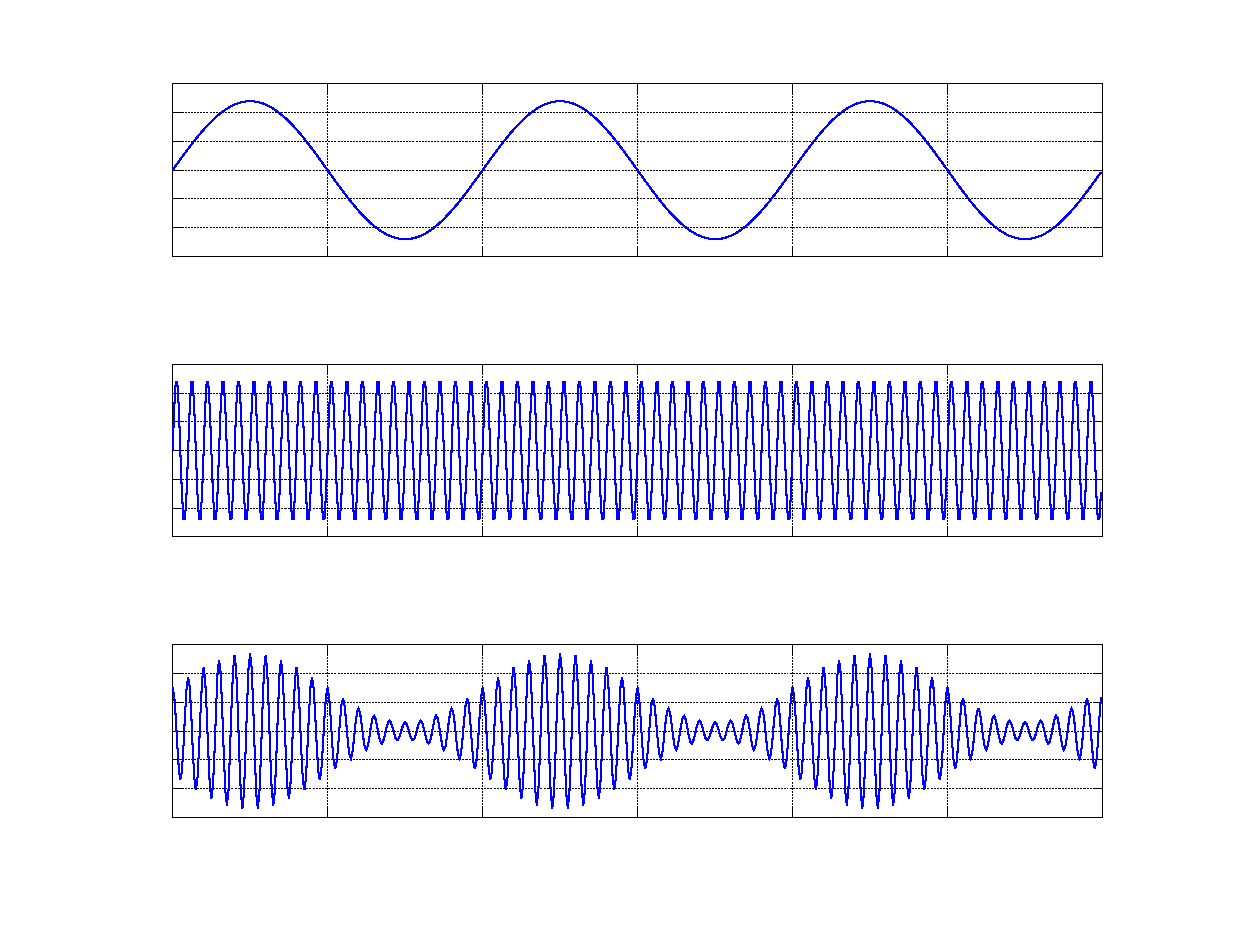
\includegraphics{am}}%
    \gplfronttext
  \end{picture}%
\endgroup
$\end{large}}
  %% Creator: Matplotlib, PGF backend
%%
%% To include the figure in your LaTeX document, write
%%   \input{<filename>.pgf}
%%
%% Make sure the required packages are loaded in your preamble
%%   \usepackage{pgf}
%%
%% Figures using additional raster images can only be included by \input if
%% they are in the same directory as the main LaTeX file. For loading figures
%% from other directories you can use the `import` package
%%   \usepackage{import}
%% and then include the figures with
%%   \import{<path to file>}{<filename>.pgf}
%%
%% Matplotlib used the following preamble
%%   \usepackage[utf8x]{inputenc}
%%   \usepackage[T1]{fontenc}
%%
\begingroup%
\makeatletter%
\begin{pgfpicture}%
\pgfpathrectangle{\pgfpointorigin}{\pgfqpoint{5.396430in}{3.335177in}}%
\pgfusepath{use as bounding box, clip}%
\begin{pgfscope}%
\pgfsetbuttcap%
\pgfsetmiterjoin%
\definecolor{currentfill}{rgb}{1.000000,1.000000,1.000000}%
\pgfsetfillcolor{currentfill}%
\pgfsetlinewidth{0.000000pt}%
\definecolor{currentstroke}{rgb}{1.000000,1.000000,1.000000}%
\pgfsetstrokecolor{currentstroke}%
\pgfsetdash{}{0pt}%
\pgfpathmoveto{\pgfqpoint{0.000000in}{0.000000in}}%
\pgfpathlineto{\pgfqpoint{5.396430in}{0.000000in}}%
\pgfpathlineto{\pgfqpoint{5.396430in}{3.335177in}}%
\pgfpathlineto{\pgfqpoint{0.000000in}{3.335177in}}%
\pgfpathclose%
\pgfusepath{fill}%
\end{pgfscope}%
\begin{pgfscope}%
\pgfsetbuttcap%
\pgfsetmiterjoin%
\definecolor{currentfill}{rgb}{1.000000,1.000000,1.000000}%
\pgfsetfillcolor{currentfill}%
\pgfsetlinewidth{0.000000pt}%
\definecolor{currentstroke}{rgb}{0.000000,0.000000,0.000000}%
\pgfsetstrokecolor{currentstroke}%
\pgfsetstrokeopacity{0.000000}%
\pgfsetdash{}{0pt}%
\pgfpathmoveto{\pgfqpoint{0.557102in}{2.631761in}}%
\pgfpathlineto{\pgfqpoint{5.305874in}{2.631761in}}%
\pgfpathlineto{\pgfqpoint{5.305874in}{3.110198in}}%
\pgfpathlineto{\pgfqpoint{0.557102in}{3.110198in}}%
\pgfpathclose%
\pgfusepath{fill}%
\end{pgfscope}%
\begin{pgfscope}%
\pgfpathrectangle{\pgfqpoint{0.557102in}{2.631761in}}{\pgfqpoint{4.748773in}{0.478437in}} %
\pgfusepath{clip}%
\pgfsetbuttcap%
\pgfsetroundjoin%
\pgfsetlinewidth{0.501875pt}%
\definecolor{currentstroke}{rgb}{0.000000,0.000000,0.000000}%
\pgfsetstrokecolor{currentstroke}%
\pgfsetstrokeopacity{0.500000}%
\pgfsetdash{{2.200000pt}{2.200000pt}}{0.000000pt}%
\pgfpathmoveto{\pgfqpoint{0.557102in}{2.631761in}}%
\pgfpathlineto{\pgfqpoint{0.557102in}{3.110198in}}%
\pgfusepath{stroke}%
\end{pgfscope}%
\begin{pgfscope}%
\pgfsetbuttcap%
\pgfsetroundjoin%
\definecolor{currentfill}{rgb}{0.000000,0.000000,0.000000}%
\pgfsetfillcolor{currentfill}%
\pgfsetlinewidth{0.803000pt}%
\definecolor{currentstroke}{rgb}{0.000000,0.000000,0.000000}%
\pgfsetstrokecolor{currentstroke}%
\pgfsetdash{}{0pt}%
\pgfsys@defobject{currentmarker}{\pgfqpoint{0.000000in}{-0.048611in}}{\pgfqpoint{0.000000in}{0.000000in}}{%
\pgfpathmoveto{\pgfqpoint{0.000000in}{0.000000in}}%
\pgfpathlineto{\pgfqpoint{0.000000in}{-0.048611in}}%
\pgfusepath{stroke,fill}%
}%
\begin{pgfscope}%
\pgfsys@transformshift{0.557102in}{2.631761in}%
\pgfsys@useobject{currentmarker}{}%
\end{pgfscope}%
\end{pgfscope}%
\begin{pgfscope}%
\pgftext[x=0.557102in,y=2.534539in,,top]{\rmfamily\fontsize{8.000000}{9.600000}\selectfont \(\displaystyle 0.00\)}%
\end{pgfscope}%
\begin{pgfscope}%
\pgfpathrectangle{\pgfqpoint{0.557102in}{2.631761in}}{\pgfqpoint{4.748773in}{0.478437in}} %
\pgfusepath{clip}%
\pgfsetbuttcap%
\pgfsetroundjoin%
\pgfsetlinewidth{0.501875pt}%
\definecolor{currentstroke}{rgb}{0.000000,0.000000,0.000000}%
\pgfsetstrokecolor{currentstroke}%
\pgfsetstrokeopacity{0.500000}%
\pgfsetdash{{2.200000pt}{2.200000pt}}{0.000000pt}%
\pgfpathmoveto{\pgfqpoint{1.349885in}{2.631761in}}%
\pgfpathlineto{\pgfqpoint{1.349885in}{3.110198in}}%
\pgfusepath{stroke}%
\end{pgfscope}%
\begin{pgfscope}%
\pgfsetbuttcap%
\pgfsetroundjoin%
\definecolor{currentfill}{rgb}{0.000000,0.000000,0.000000}%
\pgfsetfillcolor{currentfill}%
\pgfsetlinewidth{0.803000pt}%
\definecolor{currentstroke}{rgb}{0.000000,0.000000,0.000000}%
\pgfsetstrokecolor{currentstroke}%
\pgfsetdash{}{0pt}%
\pgfsys@defobject{currentmarker}{\pgfqpoint{0.000000in}{-0.048611in}}{\pgfqpoint{0.000000in}{0.000000in}}{%
\pgfpathmoveto{\pgfqpoint{0.000000in}{0.000000in}}%
\pgfpathlineto{\pgfqpoint{0.000000in}{-0.048611in}}%
\pgfusepath{stroke,fill}%
}%
\begin{pgfscope}%
\pgfsys@transformshift{1.349885in}{2.631761in}%
\pgfsys@useobject{currentmarker}{}%
\end{pgfscope}%
\end{pgfscope}%
\begin{pgfscope}%
\pgftext[x=1.349885in,y=2.534539in,,top]{\rmfamily\fontsize{8.000000}{9.600000}\selectfont \(\displaystyle 0.01\)}%
\end{pgfscope}%
\begin{pgfscope}%
\pgfpathrectangle{\pgfqpoint{0.557102in}{2.631761in}}{\pgfqpoint{4.748773in}{0.478437in}} %
\pgfusepath{clip}%
\pgfsetbuttcap%
\pgfsetroundjoin%
\pgfsetlinewidth{0.501875pt}%
\definecolor{currentstroke}{rgb}{0.000000,0.000000,0.000000}%
\pgfsetstrokecolor{currentstroke}%
\pgfsetstrokeopacity{0.500000}%
\pgfsetdash{{2.200000pt}{2.200000pt}}{0.000000pt}%
\pgfpathmoveto{\pgfqpoint{2.142669in}{2.631761in}}%
\pgfpathlineto{\pgfqpoint{2.142669in}{3.110198in}}%
\pgfusepath{stroke}%
\end{pgfscope}%
\begin{pgfscope}%
\pgfsetbuttcap%
\pgfsetroundjoin%
\definecolor{currentfill}{rgb}{0.000000,0.000000,0.000000}%
\pgfsetfillcolor{currentfill}%
\pgfsetlinewidth{0.803000pt}%
\definecolor{currentstroke}{rgb}{0.000000,0.000000,0.000000}%
\pgfsetstrokecolor{currentstroke}%
\pgfsetdash{}{0pt}%
\pgfsys@defobject{currentmarker}{\pgfqpoint{0.000000in}{-0.048611in}}{\pgfqpoint{0.000000in}{0.000000in}}{%
\pgfpathmoveto{\pgfqpoint{0.000000in}{0.000000in}}%
\pgfpathlineto{\pgfqpoint{0.000000in}{-0.048611in}}%
\pgfusepath{stroke,fill}%
}%
\begin{pgfscope}%
\pgfsys@transformshift{2.142669in}{2.631761in}%
\pgfsys@useobject{currentmarker}{}%
\end{pgfscope}%
\end{pgfscope}%
\begin{pgfscope}%
\pgftext[x=2.142669in,y=2.534539in,,top]{\rmfamily\fontsize{8.000000}{9.600000}\selectfont \(\displaystyle 0.02\)}%
\end{pgfscope}%
\begin{pgfscope}%
\pgfpathrectangle{\pgfqpoint{0.557102in}{2.631761in}}{\pgfqpoint{4.748773in}{0.478437in}} %
\pgfusepath{clip}%
\pgfsetbuttcap%
\pgfsetroundjoin%
\pgfsetlinewidth{0.501875pt}%
\definecolor{currentstroke}{rgb}{0.000000,0.000000,0.000000}%
\pgfsetstrokecolor{currentstroke}%
\pgfsetstrokeopacity{0.500000}%
\pgfsetdash{{2.200000pt}{2.200000pt}}{0.000000pt}%
\pgfpathmoveto{\pgfqpoint{2.935452in}{2.631761in}}%
\pgfpathlineto{\pgfqpoint{2.935452in}{3.110198in}}%
\pgfusepath{stroke}%
\end{pgfscope}%
\begin{pgfscope}%
\pgfsetbuttcap%
\pgfsetroundjoin%
\definecolor{currentfill}{rgb}{0.000000,0.000000,0.000000}%
\pgfsetfillcolor{currentfill}%
\pgfsetlinewidth{0.803000pt}%
\definecolor{currentstroke}{rgb}{0.000000,0.000000,0.000000}%
\pgfsetstrokecolor{currentstroke}%
\pgfsetdash{}{0pt}%
\pgfsys@defobject{currentmarker}{\pgfqpoint{0.000000in}{-0.048611in}}{\pgfqpoint{0.000000in}{0.000000in}}{%
\pgfpathmoveto{\pgfqpoint{0.000000in}{0.000000in}}%
\pgfpathlineto{\pgfqpoint{0.000000in}{-0.048611in}}%
\pgfusepath{stroke,fill}%
}%
\begin{pgfscope}%
\pgfsys@transformshift{2.935452in}{2.631761in}%
\pgfsys@useobject{currentmarker}{}%
\end{pgfscope}%
\end{pgfscope}%
\begin{pgfscope}%
\pgftext[x=2.935452in,y=2.534539in,,top]{\rmfamily\fontsize{8.000000}{9.600000}\selectfont \(\displaystyle 0.03\)}%
\end{pgfscope}%
\begin{pgfscope}%
\pgfpathrectangle{\pgfqpoint{0.557102in}{2.631761in}}{\pgfqpoint{4.748773in}{0.478437in}} %
\pgfusepath{clip}%
\pgfsetbuttcap%
\pgfsetroundjoin%
\pgfsetlinewidth{0.501875pt}%
\definecolor{currentstroke}{rgb}{0.000000,0.000000,0.000000}%
\pgfsetstrokecolor{currentstroke}%
\pgfsetstrokeopacity{0.500000}%
\pgfsetdash{{2.200000pt}{2.200000pt}}{0.000000pt}%
\pgfpathmoveto{\pgfqpoint{3.728235in}{2.631761in}}%
\pgfpathlineto{\pgfqpoint{3.728235in}{3.110198in}}%
\pgfusepath{stroke}%
\end{pgfscope}%
\begin{pgfscope}%
\pgfsetbuttcap%
\pgfsetroundjoin%
\definecolor{currentfill}{rgb}{0.000000,0.000000,0.000000}%
\pgfsetfillcolor{currentfill}%
\pgfsetlinewidth{0.803000pt}%
\definecolor{currentstroke}{rgb}{0.000000,0.000000,0.000000}%
\pgfsetstrokecolor{currentstroke}%
\pgfsetdash{}{0pt}%
\pgfsys@defobject{currentmarker}{\pgfqpoint{0.000000in}{-0.048611in}}{\pgfqpoint{0.000000in}{0.000000in}}{%
\pgfpathmoveto{\pgfqpoint{0.000000in}{0.000000in}}%
\pgfpathlineto{\pgfqpoint{0.000000in}{-0.048611in}}%
\pgfusepath{stroke,fill}%
}%
\begin{pgfscope}%
\pgfsys@transformshift{3.728235in}{2.631761in}%
\pgfsys@useobject{currentmarker}{}%
\end{pgfscope}%
\end{pgfscope}%
\begin{pgfscope}%
\pgftext[x=3.728235in,y=2.534539in,,top]{\rmfamily\fontsize{8.000000}{9.600000}\selectfont \(\displaystyle 0.04\)}%
\end{pgfscope}%
\begin{pgfscope}%
\pgfpathrectangle{\pgfqpoint{0.557102in}{2.631761in}}{\pgfqpoint{4.748773in}{0.478437in}} %
\pgfusepath{clip}%
\pgfsetbuttcap%
\pgfsetroundjoin%
\pgfsetlinewidth{0.501875pt}%
\definecolor{currentstroke}{rgb}{0.000000,0.000000,0.000000}%
\pgfsetstrokecolor{currentstroke}%
\pgfsetstrokeopacity{0.500000}%
\pgfsetdash{{2.200000pt}{2.200000pt}}{0.000000pt}%
\pgfpathmoveto{\pgfqpoint{4.521019in}{2.631761in}}%
\pgfpathlineto{\pgfqpoint{4.521019in}{3.110198in}}%
\pgfusepath{stroke}%
\end{pgfscope}%
\begin{pgfscope}%
\pgfsetbuttcap%
\pgfsetroundjoin%
\definecolor{currentfill}{rgb}{0.000000,0.000000,0.000000}%
\pgfsetfillcolor{currentfill}%
\pgfsetlinewidth{0.803000pt}%
\definecolor{currentstroke}{rgb}{0.000000,0.000000,0.000000}%
\pgfsetstrokecolor{currentstroke}%
\pgfsetdash{}{0pt}%
\pgfsys@defobject{currentmarker}{\pgfqpoint{0.000000in}{-0.048611in}}{\pgfqpoint{0.000000in}{0.000000in}}{%
\pgfpathmoveto{\pgfqpoint{0.000000in}{0.000000in}}%
\pgfpathlineto{\pgfqpoint{0.000000in}{-0.048611in}}%
\pgfusepath{stroke,fill}%
}%
\begin{pgfscope}%
\pgfsys@transformshift{4.521019in}{2.631761in}%
\pgfsys@useobject{currentmarker}{}%
\end{pgfscope}%
\end{pgfscope}%
\begin{pgfscope}%
\pgftext[x=4.521019in,y=2.534539in,,top]{\rmfamily\fontsize{8.000000}{9.600000}\selectfont \(\displaystyle 0.05\)}%
\end{pgfscope}%
\begin{pgfscope}%
\pgftext[x=2.931488in,y=2.380859in,,top]{\rmfamily\fontsize{10.000000}{12.000000}\selectfont \(\displaystyle t/s\)}%
\end{pgfscope}%
\begin{pgfscope}%
\pgfpathrectangle{\pgfqpoint{0.557102in}{2.631761in}}{\pgfqpoint{4.748773in}{0.478437in}} %
\pgfusepath{clip}%
\pgfsetbuttcap%
\pgfsetroundjoin%
\pgfsetlinewidth{0.501875pt}%
\definecolor{currentstroke}{rgb}{0.000000,0.000000,0.000000}%
\pgfsetstrokecolor{currentstroke}%
\pgfsetstrokeopacity{0.500000}%
\pgfsetdash{{2.200000pt}{2.200000pt}}{0.000000pt}%
\pgfpathmoveto{\pgfqpoint{0.557102in}{2.711500in}}%
\pgfpathlineto{\pgfqpoint{5.305874in}{2.711500in}}%
\pgfusepath{stroke}%
\end{pgfscope}%
\begin{pgfscope}%
\pgfsetbuttcap%
\pgfsetroundjoin%
\definecolor{currentfill}{rgb}{0.000000,0.000000,0.000000}%
\pgfsetfillcolor{currentfill}%
\pgfsetlinewidth{0.803000pt}%
\definecolor{currentstroke}{rgb}{0.000000,0.000000,0.000000}%
\pgfsetstrokecolor{currentstroke}%
\pgfsetdash{}{0pt}%
\pgfsys@defobject{currentmarker}{\pgfqpoint{-0.048611in}{0.000000in}}{\pgfqpoint{0.000000in}{0.000000in}}{%
\pgfpathmoveto{\pgfqpoint{0.000000in}{0.000000in}}%
\pgfpathlineto{\pgfqpoint{-0.048611in}{0.000000in}}%
\pgfusepath{stroke,fill}%
}%
\begin{pgfscope}%
\pgfsys@transformshift{0.557102in}{2.711500in}%
\pgfsys@useobject{currentmarker}{}%
\end{pgfscope}%
\end{pgfscope}%
\begin{pgfscope}%
\pgftext[x=0.250000in,y=2.673238in,left,base]{\rmfamily\fontsize{8.000000}{9.600000}\selectfont \(\displaystyle -10\)}%
\end{pgfscope}%
\begin{pgfscope}%
\pgfpathrectangle{\pgfqpoint{0.557102in}{2.631761in}}{\pgfqpoint{4.748773in}{0.478437in}} %
\pgfusepath{clip}%
\pgfsetbuttcap%
\pgfsetroundjoin%
\pgfsetlinewidth{0.501875pt}%
\definecolor{currentstroke}{rgb}{0.000000,0.000000,0.000000}%
\pgfsetstrokecolor{currentstroke}%
\pgfsetstrokeopacity{0.500000}%
\pgfsetdash{{2.200000pt}{2.200000pt}}{0.000000pt}%
\pgfpathmoveto{\pgfqpoint{0.557102in}{2.870980in}}%
\pgfpathlineto{\pgfqpoint{5.305874in}{2.870980in}}%
\pgfusepath{stroke}%
\end{pgfscope}%
\begin{pgfscope}%
\pgfsetbuttcap%
\pgfsetroundjoin%
\definecolor{currentfill}{rgb}{0.000000,0.000000,0.000000}%
\pgfsetfillcolor{currentfill}%
\pgfsetlinewidth{0.803000pt}%
\definecolor{currentstroke}{rgb}{0.000000,0.000000,0.000000}%
\pgfsetstrokecolor{currentstroke}%
\pgfsetdash{}{0pt}%
\pgfsys@defobject{currentmarker}{\pgfqpoint{-0.048611in}{0.000000in}}{\pgfqpoint{0.000000in}{0.000000in}}{%
\pgfpathmoveto{\pgfqpoint{0.000000in}{0.000000in}}%
\pgfpathlineto{\pgfqpoint{-0.048611in}{0.000000in}}%
\pgfusepath{stroke,fill}%
}%
\begin{pgfscope}%
\pgfsys@transformshift{0.557102in}{2.870980in}%
\pgfsys@useobject{currentmarker}{}%
\end{pgfscope}%
\end{pgfscope}%
\begin{pgfscope}%
\pgftext[x=0.400851in,y=2.832717in,left,base]{\rmfamily\fontsize{8.000000}{9.600000}\selectfont \(\displaystyle 0\)}%
\end{pgfscope}%
\begin{pgfscope}%
\pgfpathrectangle{\pgfqpoint{0.557102in}{2.631761in}}{\pgfqpoint{4.748773in}{0.478437in}} %
\pgfusepath{clip}%
\pgfsetbuttcap%
\pgfsetroundjoin%
\pgfsetlinewidth{0.501875pt}%
\definecolor{currentstroke}{rgb}{0.000000,0.000000,0.000000}%
\pgfsetstrokecolor{currentstroke}%
\pgfsetstrokeopacity{0.500000}%
\pgfsetdash{{2.200000pt}{2.200000pt}}{0.000000pt}%
\pgfpathmoveto{\pgfqpoint{0.557102in}{3.030459in}}%
\pgfpathlineto{\pgfqpoint{5.305874in}{3.030459in}}%
\pgfusepath{stroke}%
\end{pgfscope}%
\begin{pgfscope}%
\pgfsetbuttcap%
\pgfsetroundjoin%
\definecolor{currentfill}{rgb}{0.000000,0.000000,0.000000}%
\pgfsetfillcolor{currentfill}%
\pgfsetlinewidth{0.803000pt}%
\definecolor{currentstroke}{rgb}{0.000000,0.000000,0.000000}%
\pgfsetstrokecolor{currentstroke}%
\pgfsetdash{}{0pt}%
\pgfsys@defobject{currentmarker}{\pgfqpoint{-0.048611in}{0.000000in}}{\pgfqpoint{0.000000in}{0.000000in}}{%
\pgfpathmoveto{\pgfqpoint{0.000000in}{0.000000in}}%
\pgfpathlineto{\pgfqpoint{-0.048611in}{0.000000in}}%
\pgfusepath{stroke,fill}%
}%
\begin{pgfscope}%
\pgfsys@transformshift{0.557102in}{3.030459in}%
\pgfsys@useobject{currentmarker}{}%
\end{pgfscope}%
\end{pgfscope}%
\begin{pgfscope}%
\pgftext[x=0.341822in,y=2.992196in,left,base]{\rmfamily\fontsize{8.000000}{9.600000}\selectfont \(\displaystyle 10\)}%
\end{pgfscope}%
\begin{pgfscope}%
\pgftext[x=0.194444in,y=2.870980in,,bottom,rotate=90.000000]{\rmfamily\fontsize{10.000000}{12.000000}\selectfont \(\displaystyle u_{m}/V\)}%
\end{pgfscope}%
\begin{pgfscope}%
\pgfpathrectangle{\pgfqpoint{0.557102in}{2.631761in}}{\pgfqpoint{4.748773in}{0.478437in}} %
\pgfusepath{clip}%
\pgfsetrectcap%
\pgfsetroundjoin%
\pgfsetlinewidth{0.752812pt}%
\definecolor{currentstroke}{rgb}{0.121569,0.466667,0.705882}%
\pgfsetstrokecolor{currentstroke}%
\pgfsetdash{}{0pt}%
\pgfpathmoveto{\pgfqpoint{0.557102in}{2.870980in}}%
\pgfpathlineto{\pgfqpoint{0.644308in}{2.935805in}}%
\pgfpathlineto{\pgfqpoint{0.691875in}{2.968397in}}%
\pgfpathlineto{\pgfqpoint{0.731514in}{2.992967in}}%
\pgfpathlineto{\pgfqpoint{0.763225in}{3.010486in}}%
\pgfpathlineto{\pgfqpoint{0.794937in}{3.025805in}}%
\pgfpathlineto{\pgfqpoint{0.826648in}{3.038683in}}%
\pgfpathlineto{\pgfqpoint{0.858360in}{3.048915in}}%
\pgfpathlineto{\pgfqpoint{0.890071in}{3.056342in}}%
\pgfpathlineto{\pgfqpoint{0.921782in}{3.060845in}}%
\pgfpathlineto{\pgfqpoint{0.945566in}{3.062260in}}%
\pgfpathlineto{\pgfqpoint{0.969349in}{3.061977in}}%
\pgfpathlineto{\pgfqpoint{0.993133in}{3.059998in}}%
\pgfpathlineto{\pgfqpoint{1.024844in}{3.054756in}}%
\pgfpathlineto{\pgfqpoint{1.056555in}{3.046615in}}%
\pgfpathlineto{\pgfqpoint{1.088267in}{3.035704in}}%
\pgfpathlineto{\pgfqpoint{1.119978in}{3.022195in}}%
\pgfpathlineto{\pgfqpoint{1.151689in}{3.006302in}}%
\pgfpathlineto{\pgfqpoint{1.191329in}{2.983467in}}%
\pgfpathlineto{\pgfqpoint{1.230968in}{2.957862in}}%
\pgfpathlineto{\pgfqpoint{1.278535in}{2.924371in}}%
\pgfpathlineto{\pgfqpoint{1.349885in}{2.870980in}}%
\pgfpathlineto{\pgfqpoint{1.437091in}{2.806154in}}%
\pgfpathlineto{\pgfqpoint{1.484658in}{2.773562in}}%
\pgfpathlineto{\pgfqpoint{1.524298in}{2.748993in}}%
\pgfpathlineto{\pgfqpoint{1.556009in}{2.731473in}}%
\pgfpathlineto{\pgfqpoint{1.587720in}{2.716154in}}%
\pgfpathlineto{\pgfqpoint{1.619432in}{2.703276in}}%
\pgfpathlineto{\pgfqpoint{1.651143in}{2.693044in}}%
\pgfpathlineto{\pgfqpoint{1.682854in}{2.685617in}}%
\pgfpathlineto{\pgfqpoint{1.714566in}{2.681114in}}%
\pgfpathlineto{\pgfqpoint{1.738349in}{2.679699in}}%
\pgfpathlineto{\pgfqpoint{1.762133in}{2.679982in}}%
\pgfpathlineto{\pgfqpoint{1.785916in}{2.681961in}}%
\pgfpathlineto{\pgfqpoint{1.817627in}{2.687203in}}%
\pgfpathlineto{\pgfqpoint{1.849339in}{2.695344in}}%
\pgfpathlineto{\pgfqpoint{1.881050in}{2.706255in}}%
\pgfpathlineto{\pgfqpoint{1.912761in}{2.719764in}}%
\pgfpathlineto{\pgfqpoint{1.944473in}{2.735657in}}%
\pgfpathlineto{\pgfqpoint{1.984112in}{2.758492in}}%
\pgfpathlineto{\pgfqpoint{2.023751in}{2.784097in}}%
\pgfpathlineto{\pgfqpoint{2.071318in}{2.817588in}}%
\pgfpathlineto{\pgfqpoint{2.142669in}{2.870980in}}%
\pgfpathlineto{\pgfqpoint{2.229875in}{2.935805in}}%
\pgfpathlineto{\pgfqpoint{2.277442in}{2.968397in}}%
\pgfpathlineto{\pgfqpoint{2.317081in}{2.992967in}}%
\pgfpathlineto{\pgfqpoint{2.348792in}{3.010486in}}%
\pgfpathlineto{\pgfqpoint{2.380504in}{3.025805in}}%
\pgfpathlineto{\pgfqpoint{2.412215in}{3.038683in}}%
\pgfpathlineto{\pgfqpoint{2.443926in}{3.048915in}}%
\pgfpathlineto{\pgfqpoint{2.475638in}{3.056342in}}%
\pgfpathlineto{\pgfqpoint{2.507349in}{3.060845in}}%
\pgfpathlineto{\pgfqpoint{2.531133in}{3.062260in}}%
\pgfpathlineto{\pgfqpoint{2.554916in}{3.061977in}}%
\pgfpathlineto{\pgfqpoint{2.578700in}{3.059998in}}%
\pgfpathlineto{\pgfqpoint{2.610411in}{3.054756in}}%
\pgfpathlineto{\pgfqpoint{2.642122in}{3.046615in}}%
\pgfpathlineto{\pgfqpoint{2.673834in}{3.035704in}}%
\pgfpathlineto{\pgfqpoint{2.705545in}{3.022195in}}%
\pgfpathlineto{\pgfqpoint{2.737256in}{3.006302in}}%
\pgfpathlineto{\pgfqpoint{2.776895in}{2.983467in}}%
\pgfpathlineto{\pgfqpoint{2.816535in}{2.957862in}}%
\pgfpathlineto{\pgfqpoint{2.864102in}{2.924371in}}%
\pgfpathlineto{\pgfqpoint{2.935452in}{2.870980in}}%
\pgfpathlineto{\pgfqpoint{3.022658in}{2.806154in}}%
\pgfpathlineto{\pgfqpoint{3.070225in}{2.773562in}}%
\pgfpathlineto{\pgfqpoint{3.109864in}{2.748993in}}%
\pgfpathlineto{\pgfqpoint{3.141576in}{2.731473in}}%
\pgfpathlineto{\pgfqpoint{3.173287in}{2.716154in}}%
\pgfpathlineto{\pgfqpoint{3.204998in}{2.703276in}}%
\pgfpathlineto{\pgfqpoint{3.236710in}{2.693044in}}%
\pgfpathlineto{\pgfqpoint{3.268421in}{2.685617in}}%
\pgfpathlineto{\pgfqpoint{3.300132in}{2.681114in}}%
\pgfpathlineto{\pgfqpoint{3.323916in}{2.679699in}}%
\pgfpathlineto{\pgfqpoint{3.347699in}{2.679982in}}%
\pgfpathlineto{\pgfqpoint{3.371483in}{2.681961in}}%
\pgfpathlineto{\pgfqpoint{3.403194in}{2.687203in}}%
\pgfpathlineto{\pgfqpoint{3.434906in}{2.695344in}}%
\pgfpathlineto{\pgfqpoint{3.466617in}{2.706255in}}%
\pgfpathlineto{\pgfqpoint{3.498328in}{2.719764in}}%
\pgfpathlineto{\pgfqpoint{3.530040in}{2.735657in}}%
\pgfpathlineto{\pgfqpoint{3.569679in}{2.758492in}}%
\pgfpathlineto{\pgfqpoint{3.609318in}{2.784097in}}%
\pgfpathlineto{\pgfqpoint{3.656885in}{2.817588in}}%
\pgfpathlineto{\pgfqpoint{3.728235in}{2.870980in}}%
\pgfpathlineto{\pgfqpoint{3.815442in}{2.935805in}}%
\pgfpathlineto{\pgfqpoint{3.863009in}{2.968397in}}%
\pgfpathlineto{\pgfqpoint{3.902648in}{2.992967in}}%
\pgfpathlineto{\pgfqpoint{3.934359in}{3.010486in}}%
\pgfpathlineto{\pgfqpoint{3.966071in}{3.025805in}}%
\pgfpathlineto{\pgfqpoint{3.997782in}{3.038683in}}%
\pgfpathlineto{\pgfqpoint{4.029493in}{3.048915in}}%
\pgfpathlineto{\pgfqpoint{4.061205in}{3.056342in}}%
\pgfpathlineto{\pgfqpoint{4.092916in}{3.060845in}}%
\pgfpathlineto{\pgfqpoint{4.116699in}{3.062260in}}%
\pgfpathlineto{\pgfqpoint{4.140483in}{3.061977in}}%
\pgfpathlineto{\pgfqpoint{4.164266in}{3.059998in}}%
\pgfpathlineto{\pgfqpoint{4.195978in}{3.054756in}}%
\pgfpathlineto{\pgfqpoint{4.227689in}{3.046615in}}%
\pgfpathlineto{\pgfqpoint{4.259400in}{3.035704in}}%
\pgfpathlineto{\pgfqpoint{4.291112in}{3.022195in}}%
\pgfpathlineto{\pgfqpoint{4.322823in}{3.006302in}}%
\pgfpathlineto{\pgfqpoint{4.362462in}{2.983467in}}%
\pgfpathlineto{\pgfqpoint{4.402101in}{2.957862in}}%
\pgfpathlineto{\pgfqpoint{4.449668in}{2.924371in}}%
\pgfpathlineto{\pgfqpoint{4.521019in}{2.870980in}}%
\pgfpathlineto{\pgfqpoint{4.608225in}{2.806154in}}%
\pgfpathlineto{\pgfqpoint{4.655792in}{2.773562in}}%
\pgfpathlineto{\pgfqpoint{4.695431in}{2.748993in}}%
\pgfpathlineto{\pgfqpoint{4.727143in}{2.731473in}}%
\pgfpathlineto{\pgfqpoint{4.758854in}{2.716154in}}%
\pgfpathlineto{\pgfqpoint{4.790565in}{2.703276in}}%
\pgfpathlineto{\pgfqpoint{4.822277in}{2.693044in}}%
\pgfpathlineto{\pgfqpoint{4.853988in}{2.685617in}}%
\pgfpathlineto{\pgfqpoint{4.885699in}{2.681114in}}%
\pgfpathlineto{\pgfqpoint{4.909483in}{2.679699in}}%
\pgfpathlineto{\pgfqpoint{4.933266in}{2.679982in}}%
\pgfpathlineto{\pgfqpoint{4.957050in}{2.681961in}}%
\pgfpathlineto{\pgfqpoint{4.988761in}{2.687203in}}%
\pgfpathlineto{\pgfqpoint{5.020472in}{2.695344in}}%
\pgfpathlineto{\pgfqpoint{5.052184in}{2.706255in}}%
\pgfpathlineto{\pgfqpoint{5.083895in}{2.719764in}}%
\pgfpathlineto{\pgfqpoint{5.115606in}{2.735657in}}%
\pgfpathlineto{\pgfqpoint{5.155246in}{2.758492in}}%
\pgfpathlineto{\pgfqpoint{5.194885in}{2.784097in}}%
\pgfpathlineto{\pgfqpoint{5.242452in}{2.817588in}}%
\pgfpathlineto{\pgfqpoint{5.305874in}{2.864968in}}%
\pgfpathlineto{\pgfqpoint{5.305874in}{2.864968in}}%
\pgfusepath{stroke}%
\end{pgfscope}%
\begin{pgfscope}%
\pgfsetrectcap%
\pgfsetmiterjoin%
\pgfsetlinewidth{0.501875pt}%
\definecolor{currentstroke}{rgb}{0.000000,0.000000,0.000000}%
\pgfsetstrokecolor{currentstroke}%
\pgfsetdash{}{0pt}%
\pgfpathmoveto{\pgfqpoint{0.557102in}{2.631761in}}%
\pgfpathlineto{\pgfqpoint{0.557102in}{3.110198in}}%
\pgfusepath{stroke}%
\end{pgfscope}%
\begin{pgfscope}%
\pgfsetrectcap%
\pgfsetmiterjoin%
\pgfsetlinewidth{0.501875pt}%
\definecolor{currentstroke}{rgb}{0.000000,0.000000,0.000000}%
\pgfsetstrokecolor{currentstroke}%
\pgfsetdash{}{0pt}%
\pgfpathmoveto{\pgfqpoint{5.305874in}{2.631761in}}%
\pgfpathlineto{\pgfqpoint{5.305874in}{3.110198in}}%
\pgfusepath{stroke}%
\end{pgfscope}%
\begin{pgfscope}%
\pgfsetrectcap%
\pgfsetmiterjoin%
\pgfsetlinewidth{0.501875pt}%
\definecolor{currentstroke}{rgb}{0.000000,0.000000,0.000000}%
\pgfsetstrokecolor{currentstroke}%
\pgfsetdash{}{0pt}%
\pgfpathmoveto{\pgfqpoint{0.557102in}{2.631761in}}%
\pgfpathlineto{\pgfqpoint{5.305874in}{2.631761in}}%
\pgfusepath{stroke}%
\end{pgfscope}%
\begin{pgfscope}%
\pgfsetrectcap%
\pgfsetmiterjoin%
\pgfsetlinewidth{0.501875pt}%
\definecolor{currentstroke}{rgb}{0.000000,0.000000,0.000000}%
\pgfsetstrokecolor{currentstroke}%
\pgfsetdash{}{0pt}%
\pgfpathmoveto{\pgfqpoint{0.557102in}{3.110198in}}%
\pgfpathlineto{\pgfqpoint{5.305874in}{3.110198in}}%
\pgfusepath{stroke}%
\end{pgfscope}%
\begin{pgfscope}%
\pgftext[x=2.931488in,y=3.193531in,,base]{\rmfamily\fontsize{9.000000}{10.800000}\selectfont Nachrichtensignal}%
\end{pgfscope}%
\begin{pgfscope}%
\pgfsetbuttcap%
\pgfsetmiterjoin%
\definecolor{currentfill}{rgb}{1.000000,1.000000,1.000000}%
\pgfsetfillcolor{currentfill}%
\pgfsetlinewidth{0.000000pt}%
\definecolor{currentstroke}{rgb}{0.000000,0.000000,0.000000}%
\pgfsetstrokecolor{currentstroke}%
\pgfsetstrokeopacity{0.000000}%
\pgfsetdash{}{0pt}%
\pgfpathmoveto{\pgfqpoint{0.557102in}{1.538554in}}%
\pgfpathlineto{\pgfqpoint{5.305874in}{1.538554in}}%
\pgfpathlineto{\pgfqpoint{5.305874in}{2.016991in}}%
\pgfpathlineto{\pgfqpoint{0.557102in}{2.016991in}}%
\pgfpathclose%
\pgfusepath{fill}%
\end{pgfscope}%
\begin{pgfscope}%
\pgfpathrectangle{\pgfqpoint{0.557102in}{1.538554in}}{\pgfqpoint{4.748773in}{0.478437in}} %
\pgfusepath{clip}%
\pgfsetbuttcap%
\pgfsetroundjoin%
\pgfsetlinewidth{0.501875pt}%
\definecolor{currentstroke}{rgb}{0.000000,0.000000,0.000000}%
\pgfsetstrokecolor{currentstroke}%
\pgfsetstrokeopacity{0.500000}%
\pgfsetdash{{2.200000pt}{2.200000pt}}{0.000000pt}%
\pgfpathmoveto{\pgfqpoint{0.557102in}{1.538554in}}%
\pgfpathlineto{\pgfqpoint{0.557102in}{2.016991in}}%
\pgfusepath{stroke}%
\end{pgfscope}%
\begin{pgfscope}%
\pgfsetbuttcap%
\pgfsetroundjoin%
\definecolor{currentfill}{rgb}{0.000000,0.000000,0.000000}%
\pgfsetfillcolor{currentfill}%
\pgfsetlinewidth{0.803000pt}%
\definecolor{currentstroke}{rgb}{0.000000,0.000000,0.000000}%
\pgfsetstrokecolor{currentstroke}%
\pgfsetdash{}{0pt}%
\pgfsys@defobject{currentmarker}{\pgfqpoint{0.000000in}{-0.048611in}}{\pgfqpoint{0.000000in}{0.000000in}}{%
\pgfpathmoveto{\pgfqpoint{0.000000in}{0.000000in}}%
\pgfpathlineto{\pgfqpoint{0.000000in}{-0.048611in}}%
\pgfusepath{stroke,fill}%
}%
\begin{pgfscope}%
\pgfsys@transformshift{0.557102in}{1.538554in}%
\pgfsys@useobject{currentmarker}{}%
\end{pgfscope}%
\end{pgfscope}%
\begin{pgfscope}%
\pgftext[x=0.557102in,y=1.441332in,,top]{\rmfamily\fontsize{8.000000}{9.600000}\selectfont \(\displaystyle 0.00\)}%
\end{pgfscope}%
\begin{pgfscope}%
\pgfpathrectangle{\pgfqpoint{0.557102in}{1.538554in}}{\pgfqpoint{4.748773in}{0.478437in}} %
\pgfusepath{clip}%
\pgfsetbuttcap%
\pgfsetroundjoin%
\pgfsetlinewidth{0.501875pt}%
\definecolor{currentstroke}{rgb}{0.000000,0.000000,0.000000}%
\pgfsetstrokecolor{currentstroke}%
\pgfsetstrokeopacity{0.500000}%
\pgfsetdash{{2.200000pt}{2.200000pt}}{0.000000pt}%
\pgfpathmoveto{\pgfqpoint{1.349885in}{1.538554in}}%
\pgfpathlineto{\pgfqpoint{1.349885in}{2.016991in}}%
\pgfusepath{stroke}%
\end{pgfscope}%
\begin{pgfscope}%
\pgfsetbuttcap%
\pgfsetroundjoin%
\definecolor{currentfill}{rgb}{0.000000,0.000000,0.000000}%
\pgfsetfillcolor{currentfill}%
\pgfsetlinewidth{0.803000pt}%
\definecolor{currentstroke}{rgb}{0.000000,0.000000,0.000000}%
\pgfsetstrokecolor{currentstroke}%
\pgfsetdash{}{0pt}%
\pgfsys@defobject{currentmarker}{\pgfqpoint{0.000000in}{-0.048611in}}{\pgfqpoint{0.000000in}{0.000000in}}{%
\pgfpathmoveto{\pgfqpoint{0.000000in}{0.000000in}}%
\pgfpathlineto{\pgfqpoint{0.000000in}{-0.048611in}}%
\pgfusepath{stroke,fill}%
}%
\begin{pgfscope}%
\pgfsys@transformshift{1.349885in}{1.538554in}%
\pgfsys@useobject{currentmarker}{}%
\end{pgfscope}%
\end{pgfscope}%
\begin{pgfscope}%
\pgftext[x=1.349885in,y=1.441332in,,top]{\rmfamily\fontsize{8.000000}{9.600000}\selectfont \(\displaystyle 0.01\)}%
\end{pgfscope}%
\begin{pgfscope}%
\pgfpathrectangle{\pgfqpoint{0.557102in}{1.538554in}}{\pgfqpoint{4.748773in}{0.478437in}} %
\pgfusepath{clip}%
\pgfsetbuttcap%
\pgfsetroundjoin%
\pgfsetlinewidth{0.501875pt}%
\definecolor{currentstroke}{rgb}{0.000000,0.000000,0.000000}%
\pgfsetstrokecolor{currentstroke}%
\pgfsetstrokeopacity{0.500000}%
\pgfsetdash{{2.200000pt}{2.200000pt}}{0.000000pt}%
\pgfpathmoveto{\pgfqpoint{2.142669in}{1.538554in}}%
\pgfpathlineto{\pgfqpoint{2.142669in}{2.016991in}}%
\pgfusepath{stroke}%
\end{pgfscope}%
\begin{pgfscope}%
\pgfsetbuttcap%
\pgfsetroundjoin%
\definecolor{currentfill}{rgb}{0.000000,0.000000,0.000000}%
\pgfsetfillcolor{currentfill}%
\pgfsetlinewidth{0.803000pt}%
\definecolor{currentstroke}{rgb}{0.000000,0.000000,0.000000}%
\pgfsetstrokecolor{currentstroke}%
\pgfsetdash{}{0pt}%
\pgfsys@defobject{currentmarker}{\pgfqpoint{0.000000in}{-0.048611in}}{\pgfqpoint{0.000000in}{0.000000in}}{%
\pgfpathmoveto{\pgfqpoint{0.000000in}{0.000000in}}%
\pgfpathlineto{\pgfqpoint{0.000000in}{-0.048611in}}%
\pgfusepath{stroke,fill}%
}%
\begin{pgfscope}%
\pgfsys@transformshift{2.142669in}{1.538554in}%
\pgfsys@useobject{currentmarker}{}%
\end{pgfscope}%
\end{pgfscope}%
\begin{pgfscope}%
\pgftext[x=2.142669in,y=1.441332in,,top]{\rmfamily\fontsize{8.000000}{9.600000}\selectfont \(\displaystyle 0.02\)}%
\end{pgfscope}%
\begin{pgfscope}%
\pgfpathrectangle{\pgfqpoint{0.557102in}{1.538554in}}{\pgfqpoint{4.748773in}{0.478437in}} %
\pgfusepath{clip}%
\pgfsetbuttcap%
\pgfsetroundjoin%
\pgfsetlinewidth{0.501875pt}%
\definecolor{currentstroke}{rgb}{0.000000,0.000000,0.000000}%
\pgfsetstrokecolor{currentstroke}%
\pgfsetstrokeopacity{0.500000}%
\pgfsetdash{{2.200000pt}{2.200000pt}}{0.000000pt}%
\pgfpathmoveto{\pgfqpoint{2.935452in}{1.538554in}}%
\pgfpathlineto{\pgfqpoint{2.935452in}{2.016991in}}%
\pgfusepath{stroke}%
\end{pgfscope}%
\begin{pgfscope}%
\pgfsetbuttcap%
\pgfsetroundjoin%
\definecolor{currentfill}{rgb}{0.000000,0.000000,0.000000}%
\pgfsetfillcolor{currentfill}%
\pgfsetlinewidth{0.803000pt}%
\definecolor{currentstroke}{rgb}{0.000000,0.000000,0.000000}%
\pgfsetstrokecolor{currentstroke}%
\pgfsetdash{}{0pt}%
\pgfsys@defobject{currentmarker}{\pgfqpoint{0.000000in}{-0.048611in}}{\pgfqpoint{0.000000in}{0.000000in}}{%
\pgfpathmoveto{\pgfqpoint{0.000000in}{0.000000in}}%
\pgfpathlineto{\pgfqpoint{0.000000in}{-0.048611in}}%
\pgfusepath{stroke,fill}%
}%
\begin{pgfscope}%
\pgfsys@transformshift{2.935452in}{1.538554in}%
\pgfsys@useobject{currentmarker}{}%
\end{pgfscope}%
\end{pgfscope}%
\begin{pgfscope}%
\pgftext[x=2.935452in,y=1.441332in,,top]{\rmfamily\fontsize{8.000000}{9.600000}\selectfont \(\displaystyle 0.03\)}%
\end{pgfscope}%
\begin{pgfscope}%
\pgfpathrectangle{\pgfqpoint{0.557102in}{1.538554in}}{\pgfqpoint{4.748773in}{0.478437in}} %
\pgfusepath{clip}%
\pgfsetbuttcap%
\pgfsetroundjoin%
\pgfsetlinewidth{0.501875pt}%
\definecolor{currentstroke}{rgb}{0.000000,0.000000,0.000000}%
\pgfsetstrokecolor{currentstroke}%
\pgfsetstrokeopacity{0.500000}%
\pgfsetdash{{2.200000pt}{2.200000pt}}{0.000000pt}%
\pgfpathmoveto{\pgfqpoint{3.728235in}{1.538554in}}%
\pgfpathlineto{\pgfqpoint{3.728235in}{2.016991in}}%
\pgfusepath{stroke}%
\end{pgfscope}%
\begin{pgfscope}%
\pgfsetbuttcap%
\pgfsetroundjoin%
\definecolor{currentfill}{rgb}{0.000000,0.000000,0.000000}%
\pgfsetfillcolor{currentfill}%
\pgfsetlinewidth{0.803000pt}%
\definecolor{currentstroke}{rgb}{0.000000,0.000000,0.000000}%
\pgfsetstrokecolor{currentstroke}%
\pgfsetdash{}{0pt}%
\pgfsys@defobject{currentmarker}{\pgfqpoint{0.000000in}{-0.048611in}}{\pgfqpoint{0.000000in}{0.000000in}}{%
\pgfpathmoveto{\pgfqpoint{0.000000in}{0.000000in}}%
\pgfpathlineto{\pgfqpoint{0.000000in}{-0.048611in}}%
\pgfusepath{stroke,fill}%
}%
\begin{pgfscope}%
\pgfsys@transformshift{3.728235in}{1.538554in}%
\pgfsys@useobject{currentmarker}{}%
\end{pgfscope}%
\end{pgfscope}%
\begin{pgfscope}%
\pgftext[x=3.728235in,y=1.441332in,,top]{\rmfamily\fontsize{8.000000}{9.600000}\selectfont \(\displaystyle 0.04\)}%
\end{pgfscope}%
\begin{pgfscope}%
\pgfpathrectangle{\pgfqpoint{0.557102in}{1.538554in}}{\pgfqpoint{4.748773in}{0.478437in}} %
\pgfusepath{clip}%
\pgfsetbuttcap%
\pgfsetroundjoin%
\pgfsetlinewidth{0.501875pt}%
\definecolor{currentstroke}{rgb}{0.000000,0.000000,0.000000}%
\pgfsetstrokecolor{currentstroke}%
\pgfsetstrokeopacity{0.500000}%
\pgfsetdash{{2.200000pt}{2.200000pt}}{0.000000pt}%
\pgfpathmoveto{\pgfqpoint{4.521019in}{1.538554in}}%
\pgfpathlineto{\pgfqpoint{4.521019in}{2.016991in}}%
\pgfusepath{stroke}%
\end{pgfscope}%
\begin{pgfscope}%
\pgfsetbuttcap%
\pgfsetroundjoin%
\definecolor{currentfill}{rgb}{0.000000,0.000000,0.000000}%
\pgfsetfillcolor{currentfill}%
\pgfsetlinewidth{0.803000pt}%
\definecolor{currentstroke}{rgb}{0.000000,0.000000,0.000000}%
\pgfsetstrokecolor{currentstroke}%
\pgfsetdash{}{0pt}%
\pgfsys@defobject{currentmarker}{\pgfqpoint{0.000000in}{-0.048611in}}{\pgfqpoint{0.000000in}{0.000000in}}{%
\pgfpathmoveto{\pgfqpoint{0.000000in}{0.000000in}}%
\pgfpathlineto{\pgfqpoint{0.000000in}{-0.048611in}}%
\pgfusepath{stroke,fill}%
}%
\begin{pgfscope}%
\pgfsys@transformshift{4.521019in}{1.538554in}%
\pgfsys@useobject{currentmarker}{}%
\end{pgfscope}%
\end{pgfscope}%
\begin{pgfscope}%
\pgftext[x=4.521019in,y=1.441332in,,top]{\rmfamily\fontsize{8.000000}{9.600000}\selectfont \(\displaystyle 0.05\)}%
\end{pgfscope}%
\begin{pgfscope}%
\pgftext[x=2.931488in,y=1.287652in,,top]{\rmfamily\fontsize{10.000000}{12.000000}\selectfont \(\displaystyle t/s\)}%
\end{pgfscope}%
\begin{pgfscope}%
\pgfpathrectangle{\pgfqpoint{0.557102in}{1.538554in}}{\pgfqpoint{4.748773in}{0.478437in}} %
\pgfusepath{clip}%
\pgfsetbuttcap%
\pgfsetroundjoin%
\pgfsetlinewidth{0.501875pt}%
\definecolor{currentstroke}{rgb}{0.000000,0.000000,0.000000}%
\pgfsetstrokecolor{currentstroke}%
\pgfsetstrokeopacity{0.500000}%
\pgfsetdash{{2.200000pt}{2.200000pt}}{0.000000pt}%
\pgfpathmoveto{\pgfqpoint{0.557102in}{1.578424in}}%
\pgfpathlineto{\pgfqpoint{5.305874in}{1.578424in}}%
\pgfusepath{stroke}%
\end{pgfscope}%
\begin{pgfscope}%
\pgfsetbuttcap%
\pgfsetroundjoin%
\definecolor{currentfill}{rgb}{0.000000,0.000000,0.000000}%
\pgfsetfillcolor{currentfill}%
\pgfsetlinewidth{0.803000pt}%
\definecolor{currentstroke}{rgb}{0.000000,0.000000,0.000000}%
\pgfsetstrokecolor{currentstroke}%
\pgfsetdash{}{0pt}%
\pgfsys@defobject{currentmarker}{\pgfqpoint{-0.048611in}{0.000000in}}{\pgfqpoint{0.000000in}{0.000000in}}{%
\pgfpathmoveto{\pgfqpoint{0.000000in}{0.000000in}}%
\pgfpathlineto{\pgfqpoint{-0.048611in}{0.000000in}}%
\pgfusepath{stroke,fill}%
}%
\begin{pgfscope}%
\pgfsys@transformshift{0.557102in}{1.578424in}%
\pgfsys@useobject{currentmarker}{}%
\end{pgfscope}%
\end{pgfscope}%
\begin{pgfscope}%
\pgftext[x=0.309029in,y=1.540161in,left,base]{\rmfamily\fontsize{8.000000}{9.600000}\selectfont \(\displaystyle -5\)}%
\end{pgfscope}%
\begin{pgfscope}%
\pgfpathrectangle{\pgfqpoint{0.557102in}{1.538554in}}{\pgfqpoint{4.748773in}{0.478437in}} %
\pgfusepath{clip}%
\pgfsetbuttcap%
\pgfsetroundjoin%
\pgfsetlinewidth{0.501875pt}%
\definecolor{currentstroke}{rgb}{0.000000,0.000000,0.000000}%
\pgfsetstrokecolor{currentstroke}%
\pgfsetstrokeopacity{0.500000}%
\pgfsetdash{{2.200000pt}{2.200000pt}}{0.000000pt}%
\pgfpathmoveto{\pgfqpoint{0.557102in}{1.777772in}}%
\pgfpathlineto{\pgfqpoint{5.305874in}{1.777772in}}%
\pgfusepath{stroke}%
\end{pgfscope}%
\begin{pgfscope}%
\pgfsetbuttcap%
\pgfsetroundjoin%
\definecolor{currentfill}{rgb}{0.000000,0.000000,0.000000}%
\pgfsetfillcolor{currentfill}%
\pgfsetlinewidth{0.803000pt}%
\definecolor{currentstroke}{rgb}{0.000000,0.000000,0.000000}%
\pgfsetstrokecolor{currentstroke}%
\pgfsetdash{}{0pt}%
\pgfsys@defobject{currentmarker}{\pgfqpoint{-0.048611in}{0.000000in}}{\pgfqpoint{0.000000in}{0.000000in}}{%
\pgfpathmoveto{\pgfqpoint{0.000000in}{0.000000in}}%
\pgfpathlineto{\pgfqpoint{-0.048611in}{0.000000in}}%
\pgfusepath{stroke,fill}%
}%
\begin{pgfscope}%
\pgfsys@transformshift{0.557102in}{1.777772in}%
\pgfsys@useobject{currentmarker}{}%
\end{pgfscope}%
\end{pgfscope}%
\begin{pgfscope}%
\pgftext[x=0.400851in,y=1.739510in,left,base]{\rmfamily\fontsize{8.000000}{9.600000}\selectfont \(\displaystyle 0\)}%
\end{pgfscope}%
\begin{pgfscope}%
\pgfpathrectangle{\pgfqpoint{0.557102in}{1.538554in}}{\pgfqpoint{4.748773in}{0.478437in}} %
\pgfusepath{clip}%
\pgfsetbuttcap%
\pgfsetroundjoin%
\pgfsetlinewidth{0.501875pt}%
\definecolor{currentstroke}{rgb}{0.000000,0.000000,0.000000}%
\pgfsetstrokecolor{currentstroke}%
\pgfsetstrokeopacity{0.500000}%
\pgfsetdash{{2.200000pt}{2.200000pt}}{0.000000pt}%
\pgfpathmoveto{\pgfqpoint{0.557102in}{1.977121in}}%
\pgfpathlineto{\pgfqpoint{5.305874in}{1.977121in}}%
\pgfusepath{stroke}%
\end{pgfscope}%
\begin{pgfscope}%
\pgfsetbuttcap%
\pgfsetroundjoin%
\definecolor{currentfill}{rgb}{0.000000,0.000000,0.000000}%
\pgfsetfillcolor{currentfill}%
\pgfsetlinewidth{0.803000pt}%
\definecolor{currentstroke}{rgb}{0.000000,0.000000,0.000000}%
\pgfsetstrokecolor{currentstroke}%
\pgfsetdash{}{0pt}%
\pgfsys@defobject{currentmarker}{\pgfqpoint{-0.048611in}{0.000000in}}{\pgfqpoint{0.000000in}{0.000000in}}{%
\pgfpathmoveto{\pgfqpoint{0.000000in}{0.000000in}}%
\pgfpathlineto{\pgfqpoint{-0.048611in}{0.000000in}}%
\pgfusepath{stroke,fill}%
}%
\begin{pgfscope}%
\pgfsys@transformshift{0.557102in}{1.977121in}%
\pgfsys@useobject{currentmarker}{}%
\end{pgfscope}%
\end{pgfscope}%
\begin{pgfscope}%
\pgftext[x=0.400851in,y=1.938859in,left,base]{\rmfamily\fontsize{8.000000}{9.600000}\selectfont \(\displaystyle 5\)}%
\end{pgfscope}%
\begin{pgfscope}%
\pgftext[x=0.253473in,y=1.777772in,,bottom,rotate=90.000000]{\rmfamily\fontsize{10.000000}{12.000000}\selectfont \(\displaystyle u_{c}/V\)}%
\end{pgfscope}%
\begin{pgfscope}%
\pgfpathrectangle{\pgfqpoint{0.557102in}{1.538554in}}{\pgfqpoint{4.748773in}{0.478437in}} %
\pgfusepath{clip}%
\pgfsetrectcap%
\pgfsetroundjoin%
\pgfsetlinewidth{0.752812pt}%
\definecolor{currentstroke}{rgb}{1.000000,0.498039,0.054902}%
\pgfsetstrokecolor{currentstroke}%
\pgfsetdash{}{0pt}%
\pgfpathmoveto{\pgfqpoint{0.557102in}{1.777772in}}%
\pgfpathlineto{\pgfqpoint{0.565030in}{1.894947in}}%
\pgfpathlineto{\pgfqpoint{0.572957in}{1.967364in}}%
\pgfpathlineto{\pgfqpoint{0.580885in}{1.967364in}}%
\pgfpathlineto{\pgfqpoint{0.588813in}{1.894947in}}%
\pgfpathlineto{\pgfqpoint{0.604669in}{1.660598in}}%
\pgfpathlineto{\pgfqpoint{0.612597in}{1.588180in}}%
\pgfpathlineto{\pgfqpoint{0.620524in}{1.588180in}}%
\pgfpathlineto{\pgfqpoint{0.628452in}{1.660598in}}%
\pgfpathlineto{\pgfqpoint{0.644308in}{1.894947in}}%
\pgfpathlineto{\pgfqpoint{0.652236in}{1.967364in}}%
\pgfpathlineto{\pgfqpoint{0.660164in}{1.967364in}}%
\pgfpathlineto{\pgfqpoint{0.668091in}{1.894947in}}%
\pgfpathlineto{\pgfqpoint{0.683947in}{1.660598in}}%
\pgfpathlineto{\pgfqpoint{0.691875in}{1.588180in}}%
\pgfpathlineto{\pgfqpoint{0.699803in}{1.588180in}}%
\pgfpathlineto{\pgfqpoint{0.707731in}{1.660598in}}%
\pgfpathlineto{\pgfqpoint{0.723586in}{1.894947in}}%
\pgfpathlineto{\pgfqpoint{0.731514in}{1.967364in}}%
\pgfpathlineto{\pgfqpoint{0.739442in}{1.967364in}}%
\pgfpathlineto{\pgfqpoint{0.747370in}{1.894947in}}%
\pgfpathlineto{\pgfqpoint{0.763225in}{1.660598in}}%
\pgfpathlineto{\pgfqpoint{0.771153in}{1.588180in}}%
\pgfpathlineto{\pgfqpoint{0.779081in}{1.588180in}}%
\pgfpathlineto{\pgfqpoint{0.787009in}{1.660598in}}%
\pgfpathlineto{\pgfqpoint{0.802865in}{1.894947in}}%
\pgfpathlineto{\pgfqpoint{0.810793in}{1.967364in}}%
\pgfpathlineto{\pgfqpoint{0.818720in}{1.967364in}}%
\pgfpathlineto{\pgfqpoint{0.826648in}{1.894947in}}%
\pgfpathlineto{\pgfqpoint{0.842504in}{1.660598in}}%
\pgfpathlineto{\pgfqpoint{0.850432in}{1.588180in}}%
\pgfpathlineto{\pgfqpoint{0.858360in}{1.588180in}}%
\pgfpathlineto{\pgfqpoint{0.866287in}{1.660598in}}%
\pgfpathlineto{\pgfqpoint{0.882143in}{1.894947in}}%
\pgfpathlineto{\pgfqpoint{0.890071in}{1.967364in}}%
\pgfpathlineto{\pgfqpoint{0.897999in}{1.967364in}}%
\pgfpathlineto{\pgfqpoint{0.905927in}{1.894947in}}%
\pgfpathlineto{\pgfqpoint{0.921782in}{1.660598in}}%
\pgfpathlineto{\pgfqpoint{0.929710in}{1.588180in}}%
\pgfpathlineto{\pgfqpoint{0.937638in}{1.588180in}}%
\pgfpathlineto{\pgfqpoint{0.945566in}{1.660598in}}%
\pgfpathlineto{\pgfqpoint{0.961421in}{1.894947in}}%
\pgfpathlineto{\pgfqpoint{0.969349in}{1.967364in}}%
\pgfpathlineto{\pgfqpoint{0.977277in}{1.967364in}}%
\pgfpathlineto{\pgfqpoint{0.985205in}{1.894947in}}%
\pgfpathlineto{\pgfqpoint{1.001061in}{1.660598in}}%
\pgfpathlineto{\pgfqpoint{1.008988in}{1.588180in}}%
\pgfpathlineto{\pgfqpoint{1.016916in}{1.588180in}}%
\pgfpathlineto{\pgfqpoint{1.024844in}{1.660598in}}%
\pgfpathlineto{\pgfqpoint{1.040700in}{1.894947in}}%
\pgfpathlineto{\pgfqpoint{1.048628in}{1.967364in}}%
\pgfpathlineto{\pgfqpoint{1.056555in}{1.967364in}}%
\pgfpathlineto{\pgfqpoint{1.064483in}{1.894947in}}%
\pgfpathlineto{\pgfqpoint{1.080339in}{1.660598in}}%
\pgfpathlineto{\pgfqpoint{1.088267in}{1.588180in}}%
\pgfpathlineto{\pgfqpoint{1.096195in}{1.588180in}}%
\pgfpathlineto{\pgfqpoint{1.104122in}{1.660598in}}%
\pgfpathlineto{\pgfqpoint{1.119978in}{1.894947in}}%
\pgfpathlineto{\pgfqpoint{1.127906in}{1.967364in}}%
\pgfpathlineto{\pgfqpoint{1.135834in}{1.967364in}}%
\pgfpathlineto{\pgfqpoint{1.143762in}{1.894947in}}%
\pgfpathlineto{\pgfqpoint{1.159617in}{1.660598in}}%
\pgfpathlineto{\pgfqpoint{1.167545in}{1.588180in}}%
\pgfpathlineto{\pgfqpoint{1.175473in}{1.588180in}}%
\pgfpathlineto{\pgfqpoint{1.183401in}{1.660598in}}%
\pgfpathlineto{\pgfqpoint{1.199256in}{1.894947in}}%
\pgfpathlineto{\pgfqpoint{1.207184in}{1.967364in}}%
\pgfpathlineto{\pgfqpoint{1.215112in}{1.967364in}}%
\pgfpathlineto{\pgfqpoint{1.223040in}{1.894947in}}%
\pgfpathlineto{\pgfqpoint{1.238896in}{1.660598in}}%
\pgfpathlineto{\pgfqpoint{1.246823in}{1.588180in}}%
\pgfpathlineto{\pgfqpoint{1.254751in}{1.588180in}}%
\pgfpathlineto{\pgfqpoint{1.262679in}{1.660598in}}%
\pgfpathlineto{\pgfqpoint{1.278535in}{1.894947in}}%
\pgfpathlineto{\pgfqpoint{1.286463in}{1.967364in}}%
\pgfpathlineto{\pgfqpoint{1.294390in}{1.967364in}}%
\pgfpathlineto{\pgfqpoint{1.302318in}{1.894947in}}%
\pgfpathlineto{\pgfqpoint{1.318174in}{1.660598in}}%
\pgfpathlineto{\pgfqpoint{1.326102in}{1.588180in}}%
\pgfpathlineto{\pgfqpoint{1.334030in}{1.588180in}}%
\pgfpathlineto{\pgfqpoint{1.341957in}{1.660598in}}%
\pgfpathlineto{\pgfqpoint{1.357813in}{1.894947in}}%
\pgfpathlineto{\pgfqpoint{1.365741in}{1.967364in}}%
\pgfpathlineto{\pgfqpoint{1.373669in}{1.967364in}}%
\pgfpathlineto{\pgfqpoint{1.381597in}{1.894947in}}%
\pgfpathlineto{\pgfqpoint{1.397452in}{1.660598in}}%
\pgfpathlineto{\pgfqpoint{1.405380in}{1.588180in}}%
\pgfpathlineto{\pgfqpoint{1.413308in}{1.588180in}}%
\pgfpathlineto{\pgfqpoint{1.421236in}{1.660598in}}%
\pgfpathlineto{\pgfqpoint{1.437091in}{1.894947in}}%
\pgfpathlineto{\pgfqpoint{1.445019in}{1.967364in}}%
\pgfpathlineto{\pgfqpoint{1.452947in}{1.967364in}}%
\pgfpathlineto{\pgfqpoint{1.460875in}{1.894947in}}%
\pgfpathlineto{\pgfqpoint{1.476731in}{1.660598in}}%
\pgfpathlineto{\pgfqpoint{1.484658in}{1.588180in}}%
\pgfpathlineto{\pgfqpoint{1.492586in}{1.588180in}}%
\pgfpathlineto{\pgfqpoint{1.500514in}{1.660598in}}%
\pgfpathlineto{\pgfqpoint{1.516370in}{1.894947in}}%
\pgfpathlineto{\pgfqpoint{1.524298in}{1.967364in}}%
\pgfpathlineto{\pgfqpoint{1.532225in}{1.967364in}}%
\pgfpathlineto{\pgfqpoint{1.540153in}{1.894947in}}%
\pgfpathlineto{\pgfqpoint{1.556009in}{1.660598in}}%
\pgfpathlineto{\pgfqpoint{1.563937in}{1.588180in}}%
\pgfpathlineto{\pgfqpoint{1.571865in}{1.588180in}}%
\pgfpathlineto{\pgfqpoint{1.579792in}{1.660598in}}%
\pgfpathlineto{\pgfqpoint{1.595648in}{1.894947in}}%
\pgfpathlineto{\pgfqpoint{1.603576in}{1.967364in}}%
\pgfpathlineto{\pgfqpoint{1.611504in}{1.967364in}}%
\pgfpathlineto{\pgfqpoint{1.619432in}{1.894947in}}%
\pgfpathlineto{\pgfqpoint{1.635287in}{1.660598in}}%
\pgfpathlineto{\pgfqpoint{1.643215in}{1.588180in}}%
\pgfpathlineto{\pgfqpoint{1.651143in}{1.588180in}}%
\pgfpathlineto{\pgfqpoint{1.659071in}{1.660598in}}%
\pgfpathlineto{\pgfqpoint{1.674926in}{1.894947in}}%
\pgfpathlineto{\pgfqpoint{1.682854in}{1.967364in}}%
\pgfpathlineto{\pgfqpoint{1.690782in}{1.967364in}}%
\pgfpathlineto{\pgfqpoint{1.698710in}{1.894947in}}%
\pgfpathlineto{\pgfqpoint{1.714566in}{1.660598in}}%
\pgfpathlineto{\pgfqpoint{1.722493in}{1.588180in}}%
\pgfpathlineto{\pgfqpoint{1.730421in}{1.588180in}}%
\pgfpathlineto{\pgfqpoint{1.738349in}{1.660598in}}%
\pgfpathlineto{\pgfqpoint{1.754205in}{1.894947in}}%
\pgfpathlineto{\pgfqpoint{1.762133in}{1.967364in}}%
\pgfpathlineto{\pgfqpoint{1.770060in}{1.967364in}}%
\pgfpathlineto{\pgfqpoint{1.777988in}{1.894947in}}%
\pgfpathlineto{\pgfqpoint{1.793844in}{1.660598in}}%
\pgfpathlineto{\pgfqpoint{1.801772in}{1.588180in}}%
\pgfpathlineto{\pgfqpoint{1.809700in}{1.588180in}}%
\pgfpathlineto{\pgfqpoint{1.817627in}{1.660598in}}%
\pgfpathlineto{\pgfqpoint{1.833483in}{1.894947in}}%
\pgfpathlineto{\pgfqpoint{1.841411in}{1.967364in}}%
\pgfpathlineto{\pgfqpoint{1.849339in}{1.967364in}}%
\pgfpathlineto{\pgfqpoint{1.857267in}{1.894947in}}%
\pgfpathlineto{\pgfqpoint{1.873122in}{1.660598in}}%
\pgfpathlineto{\pgfqpoint{1.881050in}{1.588180in}}%
\pgfpathlineto{\pgfqpoint{1.888978in}{1.588180in}}%
\pgfpathlineto{\pgfqpoint{1.896906in}{1.660598in}}%
\pgfpathlineto{\pgfqpoint{1.912761in}{1.894947in}}%
\pgfpathlineto{\pgfqpoint{1.920689in}{1.967364in}}%
\pgfpathlineto{\pgfqpoint{1.928617in}{1.967364in}}%
\pgfpathlineto{\pgfqpoint{1.936545in}{1.894947in}}%
\pgfpathlineto{\pgfqpoint{1.952401in}{1.660598in}}%
\pgfpathlineto{\pgfqpoint{1.960328in}{1.588180in}}%
\pgfpathlineto{\pgfqpoint{1.968256in}{1.588180in}}%
\pgfpathlineto{\pgfqpoint{1.976184in}{1.660598in}}%
\pgfpathlineto{\pgfqpoint{1.992040in}{1.894947in}}%
\pgfpathlineto{\pgfqpoint{1.999968in}{1.967364in}}%
\pgfpathlineto{\pgfqpoint{2.007895in}{1.967364in}}%
\pgfpathlineto{\pgfqpoint{2.015823in}{1.894947in}}%
\pgfpathlineto{\pgfqpoint{2.031679in}{1.660598in}}%
\pgfpathlineto{\pgfqpoint{2.039607in}{1.588180in}}%
\pgfpathlineto{\pgfqpoint{2.047535in}{1.588180in}}%
\pgfpathlineto{\pgfqpoint{2.055462in}{1.660598in}}%
\pgfpathlineto{\pgfqpoint{2.071318in}{1.894947in}}%
\pgfpathlineto{\pgfqpoint{2.079246in}{1.967364in}}%
\pgfpathlineto{\pgfqpoint{2.087174in}{1.967364in}}%
\pgfpathlineto{\pgfqpoint{2.095102in}{1.894947in}}%
\pgfpathlineto{\pgfqpoint{2.110957in}{1.660598in}}%
\pgfpathlineto{\pgfqpoint{2.118885in}{1.588180in}}%
\pgfpathlineto{\pgfqpoint{2.126813in}{1.588180in}}%
\pgfpathlineto{\pgfqpoint{2.134741in}{1.660598in}}%
\pgfpathlineto{\pgfqpoint{2.150596in}{1.894947in}}%
\pgfpathlineto{\pgfqpoint{2.158524in}{1.967364in}}%
\pgfpathlineto{\pgfqpoint{2.166452in}{1.967364in}}%
\pgfpathlineto{\pgfqpoint{2.174380in}{1.894947in}}%
\pgfpathlineto{\pgfqpoint{2.190236in}{1.660598in}}%
\pgfpathlineto{\pgfqpoint{2.198163in}{1.588180in}}%
\pgfpathlineto{\pgfqpoint{2.206091in}{1.588180in}}%
\pgfpathlineto{\pgfqpoint{2.214019in}{1.660598in}}%
\pgfpathlineto{\pgfqpoint{2.229875in}{1.894947in}}%
\pgfpathlineto{\pgfqpoint{2.237803in}{1.967364in}}%
\pgfpathlineto{\pgfqpoint{2.245730in}{1.967364in}}%
\pgfpathlineto{\pgfqpoint{2.253658in}{1.894947in}}%
\pgfpathlineto{\pgfqpoint{2.269514in}{1.660598in}}%
\pgfpathlineto{\pgfqpoint{2.277442in}{1.588180in}}%
\pgfpathlineto{\pgfqpoint{2.285370in}{1.588180in}}%
\pgfpathlineto{\pgfqpoint{2.293297in}{1.660598in}}%
\pgfpathlineto{\pgfqpoint{2.309153in}{1.894947in}}%
\pgfpathlineto{\pgfqpoint{2.317081in}{1.967364in}}%
\pgfpathlineto{\pgfqpoint{2.325009in}{1.967364in}}%
\pgfpathlineto{\pgfqpoint{2.332937in}{1.894947in}}%
\pgfpathlineto{\pgfqpoint{2.348792in}{1.660598in}}%
\pgfpathlineto{\pgfqpoint{2.356720in}{1.588180in}}%
\pgfpathlineto{\pgfqpoint{2.364648in}{1.588180in}}%
\pgfpathlineto{\pgfqpoint{2.372576in}{1.660598in}}%
\pgfpathlineto{\pgfqpoint{2.388432in}{1.894947in}}%
\pgfpathlineto{\pgfqpoint{2.396359in}{1.967364in}}%
\pgfpathlineto{\pgfqpoint{2.404287in}{1.967364in}}%
\pgfpathlineto{\pgfqpoint{2.412215in}{1.894947in}}%
\pgfpathlineto{\pgfqpoint{2.428071in}{1.660598in}}%
\pgfpathlineto{\pgfqpoint{2.435999in}{1.588180in}}%
\pgfpathlineto{\pgfqpoint{2.443926in}{1.588180in}}%
\pgfpathlineto{\pgfqpoint{2.451854in}{1.660598in}}%
\pgfpathlineto{\pgfqpoint{2.467710in}{1.894947in}}%
\pgfpathlineto{\pgfqpoint{2.475638in}{1.967364in}}%
\pgfpathlineto{\pgfqpoint{2.483566in}{1.967364in}}%
\pgfpathlineto{\pgfqpoint{2.491493in}{1.894947in}}%
\pgfpathlineto{\pgfqpoint{2.507349in}{1.660598in}}%
\pgfpathlineto{\pgfqpoint{2.515277in}{1.588180in}}%
\pgfpathlineto{\pgfqpoint{2.523205in}{1.588180in}}%
\pgfpathlineto{\pgfqpoint{2.531133in}{1.660598in}}%
\pgfpathlineto{\pgfqpoint{2.546988in}{1.894947in}}%
\pgfpathlineto{\pgfqpoint{2.554916in}{1.967364in}}%
\pgfpathlineto{\pgfqpoint{2.562844in}{1.967364in}}%
\pgfpathlineto{\pgfqpoint{2.570772in}{1.894947in}}%
\pgfpathlineto{\pgfqpoint{2.586627in}{1.660598in}}%
\pgfpathlineto{\pgfqpoint{2.594555in}{1.588180in}}%
\pgfpathlineto{\pgfqpoint{2.602483in}{1.588180in}}%
\pgfpathlineto{\pgfqpoint{2.610411in}{1.660598in}}%
\pgfpathlineto{\pgfqpoint{2.626267in}{1.894947in}}%
\pgfpathlineto{\pgfqpoint{2.634194in}{1.967364in}}%
\pgfpathlineto{\pgfqpoint{2.642122in}{1.967364in}}%
\pgfpathlineto{\pgfqpoint{2.650050in}{1.894947in}}%
\pgfpathlineto{\pgfqpoint{2.665906in}{1.660598in}}%
\pgfpathlineto{\pgfqpoint{2.673834in}{1.588180in}}%
\pgfpathlineto{\pgfqpoint{2.681761in}{1.588180in}}%
\pgfpathlineto{\pgfqpoint{2.689689in}{1.660598in}}%
\pgfpathlineto{\pgfqpoint{2.705545in}{1.894947in}}%
\pgfpathlineto{\pgfqpoint{2.713473in}{1.967364in}}%
\pgfpathlineto{\pgfqpoint{2.721401in}{1.967364in}}%
\pgfpathlineto{\pgfqpoint{2.729328in}{1.894947in}}%
\pgfpathlineto{\pgfqpoint{2.745184in}{1.660598in}}%
\pgfpathlineto{\pgfqpoint{2.753112in}{1.588180in}}%
\pgfpathlineto{\pgfqpoint{2.761040in}{1.588180in}}%
\pgfpathlineto{\pgfqpoint{2.768968in}{1.660598in}}%
\pgfpathlineto{\pgfqpoint{2.784823in}{1.894947in}}%
\pgfpathlineto{\pgfqpoint{2.792751in}{1.967364in}}%
\pgfpathlineto{\pgfqpoint{2.800679in}{1.967364in}}%
\pgfpathlineto{\pgfqpoint{2.808607in}{1.894947in}}%
\pgfpathlineto{\pgfqpoint{2.824462in}{1.660598in}}%
\pgfpathlineto{\pgfqpoint{2.832390in}{1.588180in}}%
\pgfpathlineto{\pgfqpoint{2.840318in}{1.588180in}}%
\pgfpathlineto{\pgfqpoint{2.848246in}{1.660598in}}%
\pgfpathlineto{\pgfqpoint{2.864102in}{1.894947in}}%
\pgfpathlineto{\pgfqpoint{2.872029in}{1.967364in}}%
\pgfpathlineto{\pgfqpoint{2.879957in}{1.967364in}}%
\pgfpathlineto{\pgfqpoint{2.887885in}{1.894947in}}%
\pgfpathlineto{\pgfqpoint{2.903741in}{1.660598in}}%
\pgfpathlineto{\pgfqpoint{2.911669in}{1.588180in}}%
\pgfpathlineto{\pgfqpoint{2.919596in}{1.588180in}}%
\pgfpathlineto{\pgfqpoint{2.927524in}{1.660598in}}%
\pgfpathlineto{\pgfqpoint{2.943380in}{1.894947in}}%
\pgfpathlineto{\pgfqpoint{2.951308in}{1.967364in}}%
\pgfpathlineto{\pgfqpoint{2.959236in}{1.967364in}}%
\pgfpathlineto{\pgfqpoint{2.967163in}{1.894947in}}%
\pgfpathlineto{\pgfqpoint{2.983019in}{1.660598in}}%
\pgfpathlineto{\pgfqpoint{2.990947in}{1.588180in}}%
\pgfpathlineto{\pgfqpoint{2.998875in}{1.588180in}}%
\pgfpathlineto{\pgfqpoint{3.006803in}{1.660598in}}%
\pgfpathlineto{\pgfqpoint{3.022658in}{1.894947in}}%
\pgfpathlineto{\pgfqpoint{3.030586in}{1.967364in}}%
\pgfpathlineto{\pgfqpoint{3.038514in}{1.967364in}}%
\pgfpathlineto{\pgfqpoint{3.046442in}{1.894947in}}%
\pgfpathlineto{\pgfqpoint{3.062297in}{1.660598in}}%
\pgfpathlineto{\pgfqpoint{3.070225in}{1.588180in}}%
\pgfpathlineto{\pgfqpoint{3.078153in}{1.588180in}}%
\pgfpathlineto{\pgfqpoint{3.086081in}{1.660598in}}%
\pgfpathlineto{\pgfqpoint{3.101937in}{1.894947in}}%
\pgfpathlineto{\pgfqpoint{3.109864in}{1.967364in}}%
\pgfpathlineto{\pgfqpoint{3.117792in}{1.967364in}}%
\pgfpathlineto{\pgfqpoint{3.125720in}{1.894947in}}%
\pgfpathlineto{\pgfqpoint{3.141576in}{1.660598in}}%
\pgfpathlineto{\pgfqpoint{3.149504in}{1.588180in}}%
\pgfpathlineto{\pgfqpoint{3.157431in}{1.588180in}}%
\pgfpathlineto{\pgfqpoint{3.165359in}{1.660598in}}%
\pgfpathlineto{\pgfqpoint{3.181215in}{1.894947in}}%
\pgfpathlineto{\pgfqpoint{3.189143in}{1.967364in}}%
\pgfpathlineto{\pgfqpoint{3.197071in}{1.967364in}}%
\pgfpathlineto{\pgfqpoint{3.204998in}{1.894947in}}%
\pgfpathlineto{\pgfqpoint{3.220854in}{1.660598in}}%
\pgfpathlineto{\pgfqpoint{3.228782in}{1.588180in}}%
\pgfpathlineto{\pgfqpoint{3.236710in}{1.588180in}}%
\pgfpathlineto{\pgfqpoint{3.244638in}{1.660598in}}%
\pgfpathlineto{\pgfqpoint{3.260493in}{1.894947in}}%
\pgfpathlineto{\pgfqpoint{3.268421in}{1.967364in}}%
\pgfpathlineto{\pgfqpoint{3.276349in}{1.967364in}}%
\pgfpathlineto{\pgfqpoint{3.284277in}{1.894947in}}%
\pgfpathlineto{\pgfqpoint{3.300132in}{1.660598in}}%
\pgfpathlineto{\pgfqpoint{3.308060in}{1.588180in}}%
\pgfpathlineto{\pgfqpoint{3.315988in}{1.588180in}}%
\pgfpathlineto{\pgfqpoint{3.323916in}{1.660598in}}%
\pgfpathlineto{\pgfqpoint{3.339772in}{1.894947in}}%
\pgfpathlineto{\pgfqpoint{3.347699in}{1.967364in}}%
\pgfpathlineto{\pgfqpoint{3.355627in}{1.967364in}}%
\pgfpathlineto{\pgfqpoint{3.363555in}{1.894947in}}%
\pgfpathlineto{\pgfqpoint{3.379411in}{1.660598in}}%
\pgfpathlineto{\pgfqpoint{3.387339in}{1.588180in}}%
\pgfpathlineto{\pgfqpoint{3.395266in}{1.588180in}}%
\pgfpathlineto{\pgfqpoint{3.403194in}{1.660598in}}%
\pgfpathlineto{\pgfqpoint{3.419050in}{1.894947in}}%
\pgfpathlineto{\pgfqpoint{3.426978in}{1.967364in}}%
\pgfpathlineto{\pgfqpoint{3.434906in}{1.967364in}}%
\pgfpathlineto{\pgfqpoint{3.442833in}{1.894947in}}%
\pgfpathlineto{\pgfqpoint{3.458689in}{1.660598in}}%
\pgfpathlineto{\pgfqpoint{3.466617in}{1.588180in}}%
\pgfpathlineto{\pgfqpoint{3.474545in}{1.588180in}}%
\pgfpathlineto{\pgfqpoint{3.482473in}{1.660598in}}%
\pgfpathlineto{\pgfqpoint{3.498328in}{1.894947in}}%
\pgfpathlineto{\pgfqpoint{3.506256in}{1.967364in}}%
\pgfpathlineto{\pgfqpoint{3.514184in}{1.967364in}}%
\pgfpathlineto{\pgfqpoint{3.522112in}{1.894947in}}%
\pgfpathlineto{\pgfqpoint{3.537967in}{1.660598in}}%
\pgfpathlineto{\pgfqpoint{3.545895in}{1.588180in}}%
\pgfpathlineto{\pgfqpoint{3.553823in}{1.588180in}}%
\pgfpathlineto{\pgfqpoint{3.561751in}{1.660598in}}%
\pgfpathlineto{\pgfqpoint{3.577607in}{1.894947in}}%
\pgfpathlineto{\pgfqpoint{3.585534in}{1.967364in}}%
\pgfpathlineto{\pgfqpoint{3.593462in}{1.967364in}}%
\pgfpathlineto{\pgfqpoint{3.601390in}{1.894947in}}%
\pgfpathlineto{\pgfqpoint{3.617246in}{1.660598in}}%
\pgfpathlineto{\pgfqpoint{3.625174in}{1.588180in}}%
\pgfpathlineto{\pgfqpoint{3.633101in}{1.588180in}}%
\pgfpathlineto{\pgfqpoint{3.641029in}{1.660598in}}%
\pgfpathlineto{\pgfqpoint{3.656885in}{1.894947in}}%
\pgfpathlineto{\pgfqpoint{3.664813in}{1.967364in}}%
\pgfpathlineto{\pgfqpoint{3.672741in}{1.967364in}}%
\pgfpathlineto{\pgfqpoint{3.680668in}{1.894947in}}%
\pgfpathlineto{\pgfqpoint{3.696524in}{1.660598in}}%
\pgfpathlineto{\pgfqpoint{3.704452in}{1.588180in}}%
\pgfpathlineto{\pgfqpoint{3.712380in}{1.588180in}}%
\pgfpathlineto{\pgfqpoint{3.720308in}{1.660598in}}%
\pgfpathlineto{\pgfqpoint{3.736163in}{1.894947in}}%
\pgfpathlineto{\pgfqpoint{3.744091in}{1.967364in}}%
\pgfpathlineto{\pgfqpoint{3.752019in}{1.967364in}}%
\pgfpathlineto{\pgfqpoint{3.759947in}{1.894947in}}%
\pgfpathlineto{\pgfqpoint{3.775802in}{1.660598in}}%
\pgfpathlineto{\pgfqpoint{3.783730in}{1.588180in}}%
\pgfpathlineto{\pgfqpoint{3.791658in}{1.588180in}}%
\pgfpathlineto{\pgfqpoint{3.799586in}{1.660598in}}%
\pgfpathlineto{\pgfqpoint{3.815442in}{1.894947in}}%
\pgfpathlineto{\pgfqpoint{3.823370in}{1.967364in}}%
\pgfpathlineto{\pgfqpoint{3.831297in}{1.967364in}}%
\pgfpathlineto{\pgfqpoint{3.839225in}{1.894947in}}%
\pgfpathlineto{\pgfqpoint{3.855081in}{1.660598in}}%
\pgfpathlineto{\pgfqpoint{3.863009in}{1.588180in}}%
\pgfpathlineto{\pgfqpoint{3.870937in}{1.588180in}}%
\pgfpathlineto{\pgfqpoint{3.878864in}{1.660598in}}%
\pgfpathlineto{\pgfqpoint{3.894720in}{1.894947in}}%
\pgfpathlineto{\pgfqpoint{3.902648in}{1.967364in}}%
\pgfpathlineto{\pgfqpoint{3.910576in}{1.967364in}}%
\pgfpathlineto{\pgfqpoint{3.918504in}{1.894947in}}%
\pgfpathlineto{\pgfqpoint{3.934359in}{1.660598in}}%
\pgfpathlineto{\pgfqpoint{3.942287in}{1.588180in}}%
\pgfpathlineto{\pgfqpoint{3.950215in}{1.588180in}}%
\pgfpathlineto{\pgfqpoint{3.958143in}{1.660598in}}%
\pgfpathlineto{\pgfqpoint{3.973998in}{1.894947in}}%
\pgfpathlineto{\pgfqpoint{3.981926in}{1.967364in}}%
\pgfpathlineto{\pgfqpoint{3.989854in}{1.967364in}}%
\pgfpathlineto{\pgfqpoint{3.997782in}{1.894947in}}%
\pgfpathlineto{\pgfqpoint{4.013638in}{1.660598in}}%
\pgfpathlineto{\pgfqpoint{4.021565in}{1.588180in}}%
\pgfpathlineto{\pgfqpoint{4.029493in}{1.588180in}}%
\pgfpathlineto{\pgfqpoint{4.037421in}{1.660598in}}%
\pgfpathlineto{\pgfqpoint{4.053277in}{1.894947in}}%
\pgfpathlineto{\pgfqpoint{4.061205in}{1.967364in}}%
\pgfpathlineto{\pgfqpoint{4.069132in}{1.967364in}}%
\pgfpathlineto{\pgfqpoint{4.077060in}{1.894947in}}%
\pgfpathlineto{\pgfqpoint{4.092916in}{1.660598in}}%
\pgfpathlineto{\pgfqpoint{4.100844in}{1.588180in}}%
\pgfpathlineto{\pgfqpoint{4.108772in}{1.588180in}}%
\pgfpathlineto{\pgfqpoint{4.116699in}{1.660598in}}%
\pgfpathlineto{\pgfqpoint{4.132555in}{1.894947in}}%
\pgfpathlineto{\pgfqpoint{4.140483in}{1.967364in}}%
\pgfpathlineto{\pgfqpoint{4.148411in}{1.967364in}}%
\pgfpathlineto{\pgfqpoint{4.156339in}{1.894947in}}%
\pgfpathlineto{\pgfqpoint{4.172194in}{1.660598in}}%
\pgfpathlineto{\pgfqpoint{4.180122in}{1.588180in}}%
\pgfpathlineto{\pgfqpoint{4.188050in}{1.588180in}}%
\pgfpathlineto{\pgfqpoint{4.195978in}{1.660598in}}%
\pgfpathlineto{\pgfqpoint{4.211833in}{1.894947in}}%
\pgfpathlineto{\pgfqpoint{4.219761in}{1.967364in}}%
\pgfpathlineto{\pgfqpoint{4.227689in}{1.967364in}}%
\pgfpathlineto{\pgfqpoint{4.235617in}{1.894947in}}%
\pgfpathlineto{\pgfqpoint{4.251473in}{1.660598in}}%
\pgfpathlineto{\pgfqpoint{4.259400in}{1.588180in}}%
\pgfpathlineto{\pgfqpoint{4.267328in}{1.588180in}}%
\pgfpathlineto{\pgfqpoint{4.275256in}{1.660598in}}%
\pgfpathlineto{\pgfqpoint{4.291112in}{1.894947in}}%
\pgfpathlineto{\pgfqpoint{4.299040in}{1.967364in}}%
\pgfpathlineto{\pgfqpoint{4.306967in}{1.967364in}}%
\pgfpathlineto{\pgfqpoint{4.314895in}{1.894947in}}%
\pgfpathlineto{\pgfqpoint{4.330751in}{1.660598in}}%
\pgfpathlineto{\pgfqpoint{4.338679in}{1.588180in}}%
\pgfpathlineto{\pgfqpoint{4.346607in}{1.588180in}}%
\pgfpathlineto{\pgfqpoint{4.354534in}{1.660598in}}%
\pgfpathlineto{\pgfqpoint{4.370390in}{1.894947in}}%
\pgfpathlineto{\pgfqpoint{4.378318in}{1.967364in}}%
\pgfpathlineto{\pgfqpoint{4.386246in}{1.967364in}}%
\pgfpathlineto{\pgfqpoint{4.394174in}{1.894947in}}%
\pgfpathlineto{\pgfqpoint{4.410029in}{1.660598in}}%
\pgfpathlineto{\pgfqpoint{4.417957in}{1.588180in}}%
\pgfpathlineto{\pgfqpoint{4.425885in}{1.588180in}}%
\pgfpathlineto{\pgfqpoint{4.433813in}{1.660598in}}%
\pgfpathlineto{\pgfqpoint{4.449668in}{1.894947in}}%
\pgfpathlineto{\pgfqpoint{4.457596in}{1.967364in}}%
\pgfpathlineto{\pgfqpoint{4.465524in}{1.967364in}}%
\pgfpathlineto{\pgfqpoint{4.473452in}{1.894947in}}%
\pgfpathlineto{\pgfqpoint{4.489308in}{1.660598in}}%
\pgfpathlineto{\pgfqpoint{4.497235in}{1.588180in}}%
\pgfpathlineto{\pgfqpoint{4.505163in}{1.588180in}}%
\pgfpathlineto{\pgfqpoint{4.513091in}{1.660598in}}%
\pgfpathlineto{\pgfqpoint{4.528947in}{1.894947in}}%
\pgfpathlineto{\pgfqpoint{4.536875in}{1.967364in}}%
\pgfpathlineto{\pgfqpoint{4.544802in}{1.967364in}}%
\pgfpathlineto{\pgfqpoint{4.552730in}{1.894947in}}%
\pgfpathlineto{\pgfqpoint{4.568586in}{1.660598in}}%
\pgfpathlineto{\pgfqpoint{4.576514in}{1.588180in}}%
\pgfpathlineto{\pgfqpoint{4.584442in}{1.588180in}}%
\pgfpathlineto{\pgfqpoint{4.592369in}{1.660598in}}%
\pgfpathlineto{\pgfqpoint{4.608225in}{1.894947in}}%
\pgfpathlineto{\pgfqpoint{4.616153in}{1.967364in}}%
\pgfpathlineto{\pgfqpoint{4.624081in}{1.967364in}}%
\pgfpathlineto{\pgfqpoint{4.632009in}{1.894947in}}%
\pgfpathlineto{\pgfqpoint{4.647864in}{1.660598in}}%
\pgfpathlineto{\pgfqpoint{4.655792in}{1.588180in}}%
\pgfpathlineto{\pgfqpoint{4.663720in}{1.588180in}}%
\pgfpathlineto{\pgfqpoint{4.671648in}{1.660598in}}%
\pgfpathlineto{\pgfqpoint{4.687503in}{1.894947in}}%
\pgfpathlineto{\pgfqpoint{4.695431in}{1.967364in}}%
\pgfpathlineto{\pgfqpoint{4.703359in}{1.967364in}}%
\pgfpathlineto{\pgfqpoint{4.711287in}{1.894947in}}%
\pgfpathlineto{\pgfqpoint{4.727143in}{1.660598in}}%
\pgfpathlineto{\pgfqpoint{4.735070in}{1.588180in}}%
\pgfpathlineto{\pgfqpoint{4.742998in}{1.588180in}}%
\pgfpathlineto{\pgfqpoint{4.750926in}{1.660598in}}%
\pgfpathlineto{\pgfqpoint{4.766782in}{1.894947in}}%
\pgfpathlineto{\pgfqpoint{4.774710in}{1.967364in}}%
\pgfpathlineto{\pgfqpoint{4.782637in}{1.967364in}}%
\pgfpathlineto{\pgfqpoint{4.790565in}{1.894947in}}%
\pgfpathlineto{\pgfqpoint{4.806421in}{1.660598in}}%
\pgfpathlineto{\pgfqpoint{4.814349in}{1.588180in}}%
\pgfpathlineto{\pgfqpoint{4.822277in}{1.588180in}}%
\pgfpathlineto{\pgfqpoint{4.830204in}{1.660598in}}%
\pgfpathlineto{\pgfqpoint{4.846060in}{1.894947in}}%
\pgfpathlineto{\pgfqpoint{4.853988in}{1.967364in}}%
\pgfpathlineto{\pgfqpoint{4.861916in}{1.967364in}}%
\pgfpathlineto{\pgfqpoint{4.869844in}{1.894947in}}%
\pgfpathlineto{\pgfqpoint{4.885699in}{1.660598in}}%
\pgfpathlineto{\pgfqpoint{4.893627in}{1.588180in}}%
\pgfpathlineto{\pgfqpoint{4.901555in}{1.588180in}}%
\pgfpathlineto{\pgfqpoint{4.909483in}{1.660598in}}%
\pgfpathlineto{\pgfqpoint{4.925338in}{1.894947in}}%
\pgfpathlineto{\pgfqpoint{4.933266in}{1.967364in}}%
\pgfpathlineto{\pgfqpoint{4.941194in}{1.967364in}}%
\pgfpathlineto{\pgfqpoint{4.949122in}{1.894947in}}%
\pgfpathlineto{\pgfqpoint{4.964978in}{1.660598in}}%
\pgfpathlineto{\pgfqpoint{4.972905in}{1.588180in}}%
\pgfpathlineto{\pgfqpoint{4.980833in}{1.588180in}}%
\pgfpathlineto{\pgfqpoint{4.988761in}{1.660598in}}%
\pgfpathlineto{\pgfqpoint{5.004617in}{1.894947in}}%
\pgfpathlineto{\pgfqpoint{5.012545in}{1.967364in}}%
\pgfpathlineto{\pgfqpoint{5.020472in}{1.967364in}}%
\pgfpathlineto{\pgfqpoint{5.028400in}{1.894947in}}%
\pgfpathlineto{\pgfqpoint{5.044256in}{1.660598in}}%
\pgfpathlineto{\pgfqpoint{5.052184in}{1.588180in}}%
\pgfpathlineto{\pgfqpoint{5.060112in}{1.588180in}}%
\pgfpathlineto{\pgfqpoint{5.068039in}{1.660598in}}%
\pgfpathlineto{\pgfqpoint{5.083895in}{1.894947in}}%
\pgfpathlineto{\pgfqpoint{5.091823in}{1.967364in}}%
\pgfpathlineto{\pgfqpoint{5.099751in}{1.967364in}}%
\pgfpathlineto{\pgfqpoint{5.107679in}{1.894947in}}%
\pgfpathlineto{\pgfqpoint{5.123534in}{1.660598in}}%
\pgfpathlineto{\pgfqpoint{5.131462in}{1.588180in}}%
\pgfpathlineto{\pgfqpoint{5.139390in}{1.588180in}}%
\pgfpathlineto{\pgfqpoint{5.147318in}{1.660598in}}%
\pgfpathlineto{\pgfqpoint{5.163173in}{1.894947in}}%
\pgfpathlineto{\pgfqpoint{5.171101in}{1.967364in}}%
\pgfpathlineto{\pgfqpoint{5.179029in}{1.967364in}}%
\pgfpathlineto{\pgfqpoint{5.186957in}{1.894947in}}%
\pgfpathlineto{\pgfqpoint{5.202813in}{1.660598in}}%
\pgfpathlineto{\pgfqpoint{5.210740in}{1.588180in}}%
\pgfpathlineto{\pgfqpoint{5.218668in}{1.588180in}}%
\pgfpathlineto{\pgfqpoint{5.226596in}{1.660598in}}%
\pgfpathlineto{\pgfqpoint{5.242452in}{1.894947in}}%
\pgfpathlineto{\pgfqpoint{5.250380in}{1.967364in}}%
\pgfpathlineto{\pgfqpoint{5.258307in}{1.967364in}}%
\pgfpathlineto{\pgfqpoint{5.266235in}{1.894947in}}%
\pgfpathlineto{\pgfqpoint{5.282091in}{1.660598in}}%
\pgfpathlineto{\pgfqpoint{5.290019in}{1.588180in}}%
\pgfpathlineto{\pgfqpoint{5.297947in}{1.588180in}}%
\pgfpathlineto{\pgfqpoint{5.305874in}{1.660598in}}%
\pgfpathlineto{\pgfqpoint{5.305874in}{1.660598in}}%
\pgfusepath{stroke}%
\end{pgfscope}%
\begin{pgfscope}%
\pgfsetrectcap%
\pgfsetmiterjoin%
\pgfsetlinewidth{0.501875pt}%
\definecolor{currentstroke}{rgb}{0.000000,0.000000,0.000000}%
\pgfsetstrokecolor{currentstroke}%
\pgfsetdash{}{0pt}%
\pgfpathmoveto{\pgfqpoint{0.557102in}{1.538554in}}%
\pgfpathlineto{\pgfqpoint{0.557102in}{2.016991in}}%
\pgfusepath{stroke}%
\end{pgfscope}%
\begin{pgfscope}%
\pgfsetrectcap%
\pgfsetmiterjoin%
\pgfsetlinewidth{0.501875pt}%
\definecolor{currentstroke}{rgb}{0.000000,0.000000,0.000000}%
\pgfsetstrokecolor{currentstroke}%
\pgfsetdash{}{0pt}%
\pgfpathmoveto{\pgfqpoint{5.305874in}{1.538554in}}%
\pgfpathlineto{\pgfqpoint{5.305874in}{2.016991in}}%
\pgfusepath{stroke}%
\end{pgfscope}%
\begin{pgfscope}%
\pgfsetrectcap%
\pgfsetmiterjoin%
\pgfsetlinewidth{0.501875pt}%
\definecolor{currentstroke}{rgb}{0.000000,0.000000,0.000000}%
\pgfsetstrokecolor{currentstroke}%
\pgfsetdash{}{0pt}%
\pgfpathmoveto{\pgfqpoint{0.557102in}{1.538554in}}%
\pgfpathlineto{\pgfqpoint{5.305874in}{1.538554in}}%
\pgfusepath{stroke}%
\end{pgfscope}%
\begin{pgfscope}%
\pgfsetrectcap%
\pgfsetmiterjoin%
\pgfsetlinewidth{0.501875pt}%
\definecolor{currentstroke}{rgb}{0.000000,0.000000,0.000000}%
\pgfsetstrokecolor{currentstroke}%
\pgfsetdash{}{0pt}%
\pgfpathmoveto{\pgfqpoint{0.557102in}{2.016991in}}%
\pgfpathlineto{\pgfqpoint{5.305874in}{2.016991in}}%
\pgfusepath{stroke}%
\end{pgfscope}%
\begin{pgfscope}%
\pgftext[x=2.931488in,y=2.100324in,,base]{\rmfamily\fontsize{9.000000}{10.800000}\selectfont Trägersignal}%
\end{pgfscope}%
\begin{pgfscope}%
\pgfsetbuttcap%
\pgfsetmiterjoin%
\definecolor{currentfill}{rgb}{1.000000,1.000000,1.000000}%
\pgfsetfillcolor{currentfill}%
\pgfsetlinewidth{0.000000pt}%
\definecolor{currentstroke}{rgb}{0.000000,0.000000,0.000000}%
\pgfsetstrokecolor{currentstroke}%
\pgfsetstrokeopacity{0.000000}%
\pgfsetdash{}{0pt}%
\pgfpathmoveto{\pgfqpoint{0.557102in}{0.445347in}}%
\pgfpathlineto{\pgfqpoint{5.305874in}{0.445347in}}%
\pgfpathlineto{\pgfqpoint{5.305874in}{0.923784in}}%
\pgfpathlineto{\pgfqpoint{0.557102in}{0.923784in}}%
\pgfpathclose%
\pgfusepath{fill}%
\end{pgfscope}%
\begin{pgfscope}%
\pgfpathrectangle{\pgfqpoint{0.557102in}{0.445347in}}{\pgfqpoint{4.748773in}{0.478437in}} %
\pgfusepath{clip}%
\pgfsetbuttcap%
\pgfsetroundjoin%
\pgfsetlinewidth{0.501875pt}%
\definecolor{currentstroke}{rgb}{0.000000,0.000000,0.000000}%
\pgfsetstrokecolor{currentstroke}%
\pgfsetstrokeopacity{0.500000}%
\pgfsetdash{{2.200000pt}{2.200000pt}}{0.000000pt}%
\pgfpathmoveto{\pgfqpoint{0.557102in}{0.445347in}}%
\pgfpathlineto{\pgfqpoint{0.557102in}{0.923784in}}%
\pgfusepath{stroke}%
\end{pgfscope}%
\begin{pgfscope}%
\pgfsetbuttcap%
\pgfsetroundjoin%
\definecolor{currentfill}{rgb}{0.000000,0.000000,0.000000}%
\pgfsetfillcolor{currentfill}%
\pgfsetlinewidth{0.803000pt}%
\definecolor{currentstroke}{rgb}{0.000000,0.000000,0.000000}%
\pgfsetstrokecolor{currentstroke}%
\pgfsetdash{}{0pt}%
\pgfsys@defobject{currentmarker}{\pgfqpoint{0.000000in}{-0.048611in}}{\pgfqpoint{0.000000in}{0.000000in}}{%
\pgfpathmoveto{\pgfqpoint{0.000000in}{0.000000in}}%
\pgfpathlineto{\pgfqpoint{0.000000in}{-0.048611in}}%
\pgfusepath{stroke,fill}%
}%
\begin{pgfscope}%
\pgfsys@transformshift{0.557102in}{0.445347in}%
\pgfsys@useobject{currentmarker}{}%
\end{pgfscope}%
\end{pgfscope}%
\begin{pgfscope}%
\pgftext[x=0.557102in,y=0.348124in,,top]{\rmfamily\fontsize{8.000000}{9.600000}\selectfont \(\displaystyle 0.00\)}%
\end{pgfscope}%
\begin{pgfscope}%
\pgfpathrectangle{\pgfqpoint{0.557102in}{0.445347in}}{\pgfqpoint{4.748773in}{0.478437in}} %
\pgfusepath{clip}%
\pgfsetbuttcap%
\pgfsetroundjoin%
\pgfsetlinewidth{0.501875pt}%
\definecolor{currentstroke}{rgb}{0.000000,0.000000,0.000000}%
\pgfsetstrokecolor{currentstroke}%
\pgfsetstrokeopacity{0.500000}%
\pgfsetdash{{2.200000pt}{2.200000pt}}{0.000000pt}%
\pgfpathmoveto{\pgfqpoint{1.349885in}{0.445347in}}%
\pgfpathlineto{\pgfqpoint{1.349885in}{0.923784in}}%
\pgfusepath{stroke}%
\end{pgfscope}%
\begin{pgfscope}%
\pgfsetbuttcap%
\pgfsetroundjoin%
\definecolor{currentfill}{rgb}{0.000000,0.000000,0.000000}%
\pgfsetfillcolor{currentfill}%
\pgfsetlinewidth{0.803000pt}%
\definecolor{currentstroke}{rgb}{0.000000,0.000000,0.000000}%
\pgfsetstrokecolor{currentstroke}%
\pgfsetdash{}{0pt}%
\pgfsys@defobject{currentmarker}{\pgfqpoint{0.000000in}{-0.048611in}}{\pgfqpoint{0.000000in}{0.000000in}}{%
\pgfpathmoveto{\pgfqpoint{0.000000in}{0.000000in}}%
\pgfpathlineto{\pgfqpoint{0.000000in}{-0.048611in}}%
\pgfusepath{stroke,fill}%
}%
\begin{pgfscope}%
\pgfsys@transformshift{1.349885in}{0.445347in}%
\pgfsys@useobject{currentmarker}{}%
\end{pgfscope}%
\end{pgfscope}%
\begin{pgfscope}%
\pgftext[x=1.349885in,y=0.348124in,,top]{\rmfamily\fontsize{8.000000}{9.600000}\selectfont \(\displaystyle 0.01\)}%
\end{pgfscope}%
\begin{pgfscope}%
\pgfpathrectangle{\pgfqpoint{0.557102in}{0.445347in}}{\pgfqpoint{4.748773in}{0.478437in}} %
\pgfusepath{clip}%
\pgfsetbuttcap%
\pgfsetroundjoin%
\pgfsetlinewidth{0.501875pt}%
\definecolor{currentstroke}{rgb}{0.000000,0.000000,0.000000}%
\pgfsetstrokecolor{currentstroke}%
\pgfsetstrokeopacity{0.500000}%
\pgfsetdash{{2.200000pt}{2.200000pt}}{0.000000pt}%
\pgfpathmoveto{\pgfqpoint{2.142669in}{0.445347in}}%
\pgfpathlineto{\pgfqpoint{2.142669in}{0.923784in}}%
\pgfusepath{stroke}%
\end{pgfscope}%
\begin{pgfscope}%
\pgfsetbuttcap%
\pgfsetroundjoin%
\definecolor{currentfill}{rgb}{0.000000,0.000000,0.000000}%
\pgfsetfillcolor{currentfill}%
\pgfsetlinewidth{0.803000pt}%
\definecolor{currentstroke}{rgb}{0.000000,0.000000,0.000000}%
\pgfsetstrokecolor{currentstroke}%
\pgfsetdash{}{0pt}%
\pgfsys@defobject{currentmarker}{\pgfqpoint{0.000000in}{-0.048611in}}{\pgfqpoint{0.000000in}{0.000000in}}{%
\pgfpathmoveto{\pgfqpoint{0.000000in}{0.000000in}}%
\pgfpathlineto{\pgfqpoint{0.000000in}{-0.048611in}}%
\pgfusepath{stroke,fill}%
}%
\begin{pgfscope}%
\pgfsys@transformshift{2.142669in}{0.445347in}%
\pgfsys@useobject{currentmarker}{}%
\end{pgfscope}%
\end{pgfscope}%
\begin{pgfscope}%
\pgftext[x=2.142669in,y=0.348124in,,top]{\rmfamily\fontsize{8.000000}{9.600000}\selectfont \(\displaystyle 0.02\)}%
\end{pgfscope}%
\begin{pgfscope}%
\pgfpathrectangle{\pgfqpoint{0.557102in}{0.445347in}}{\pgfqpoint{4.748773in}{0.478437in}} %
\pgfusepath{clip}%
\pgfsetbuttcap%
\pgfsetroundjoin%
\pgfsetlinewidth{0.501875pt}%
\definecolor{currentstroke}{rgb}{0.000000,0.000000,0.000000}%
\pgfsetstrokecolor{currentstroke}%
\pgfsetstrokeopacity{0.500000}%
\pgfsetdash{{2.200000pt}{2.200000pt}}{0.000000pt}%
\pgfpathmoveto{\pgfqpoint{2.935452in}{0.445347in}}%
\pgfpathlineto{\pgfqpoint{2.935452in}{0.923784in}}%
\pgfusepath{stroke}%
\end{pgfscope}%
\begin{pgfscope}%
\pgfsetbuttcap%
\pgfsetroundjoin%
\definecolor{currentfill}{rgb}{0.000000,0.000000,0.000000}%
\pgfsetfillcolor{currentfill}%
\pgfsetlinewidth{0.803000pt}%
\definecolor{currentstroke}{rgb}{0.000000,0.000000,0.000000}%
\pgfsetstrokecolor{currentstroke}%
\pgfsetdash{}{0pt}%
\pgfsys@defobject{currentmarker}{\pgfqpoint{0.000000in}{-0.048611in}}{\pgfqpoint{0.000000in}{0.000000in}}{%
\pgfpathmoveto{\pgfqpoint{0.000000in}{0.000000in}}%
\pgfpathlineto{\pgfqpoint{0.000000in}{-0.048611in}}%
\pgfusepath{stroke,fill}%
}%
\begin{pgfscope}%
\pgfsys@transformshift{2.935452in}{0.445347in}%
\pgfsys@useobject{currentmarker}{}%
\end{pgfscope}%
\end{pgfscope}%
\begin{pgfscope}%
\pgftext[x=2.935452in,y=0.348124in,,top]{\rmfamily\fontsize{8.000000}{9.600000}\selectfont \(\displaystyle 0.03\)}%
\end{pgfscope}%
\begin{pgfscope}%
\pgfpathrectangle{\pgfqpoint{0.557102in}{0.445347in}}{\pgfqpoint{4.748773in}{0.478437in}} %
\pgfusepath{clip}%
\pgfsetbuttcap%
\pgfsetroundjoin%
\pgfsetlinewidth{0.501875pt}%
\definecolor{currentstroke}{rgb}{0.000000,0.000000,0.000000}%
\pgfsetstrokecolor{currentstroke}%
\pgfsetstrokeopacity{0.500000}%
\pgfsetdash{{2.200000pt}{2.200000pt}}{0.000000pt}%
\pgfpathmoveto{\pgfqpoint{3.728235in}{0.445347in}}%
\pgfpathlineto{\pgfqpoint{3.728235in}{0.923784in}}%
\pgfusepath{stroke}%
\end{pgfscope}%
\begin{pgfscope}%
\pgfsetbuttcap%
\pgfsetroundjoin%
\definecolor{currentfill}{rgb}{0.000000,0.000000,0.000000}%
\pgfsetfillcolor{currentfill}%
\pgfsetlinewidth{0.803000pt}%
\definecolor{currentstroke}{rgb}{0.000000,0.000000,0.000000}%
\pgfsetstrokecolor{currentstroke}%
\pgfsetdash{}{0pt}%
\pgfsys@defobject{currentmarker}{\pgfqpoint{0.000000in}{-0.048611in}}{\pgfqpoint{0.000000in}{0.000000in}}{%
\pgfpathmoveto{\pgfqpoint{0.000000in}{0.000000in}}%
\pgfpathlineto{\pgfqpoint{0.000000in}{-0.048611in}}%
\pgfusepath{stroke,fill}%
}%
\begin{pgfscope}%
\pgfsys@transformshift{3.728235in}{0.445347in}%
\pgfsys@useobject{currentmarker}{}%
\end{pgfscope}%
\end{pgfscope}%
\begin{pgfscope}%
\pgftext[x=3.728235in,y=0.348124in,,top]{\rmfamily\fontsize{8.000000}{9.600000}\selectfont \(\displaystyle 0.04\)}%
\end{pgfscope}%
\begin{pgfscope}%
\pgfpathrectangle{\pgfqpoint{0.557102in}{0.445347in}}{\pgfqpoint{4.748773in}{0.478437in}} %
\pgfusepath{clip}%
\pgfsetbuttcap%
\pgfsetroundjoin%
\pgfsetlinewidth{0.501875pt}%
\definecolor{currentstroke}{rgb}{0.000000,0.000000,0.000000}%
\pgfsetstrokecolor{currentstroke}%
\pgfsetstrokeopacity{0.500000}%
\pgfsetdash{{2.200000pt}{2.200000pt}}{0.000000pt}%
\pgfpathmoveto{\pgfqpoint{4.521019in}{0.445347in}}%
\pgfpathlineto{\pgfqpoint{4.521019in}{0.923784in}}%
\pgfusepath{stroke}%
\end{pgfscope}%
\begin{pgfscope}%
\pgfsetbuttcap%
\pgfsetroundjoin%
\definecolor{currentfill}{rgb}{0.000000,0.000000,0.000000}%
\pgfsetfillcolor{currentfill}%
\pgfsetlinewidth{0.803000pt}%
\definecolor{currentstroke}{rgb}{0.000000,0.000000,0.000000}%
\pgfsetstrokecolor{currentstroke}%
\pgfsetdash{}{0pt}%
\pgfsys@defobject{currentmarker}{\pgfqpoint{0.000000in}{-0.048611in}}{\pgfqpoint{0.000000in}{0.000000in}}{%
\pgfpathmoveto{\pgfqpoint{0.000000in}{0.000000in}}%
\pgfpathlineto{\pgfqpoint{0.000000in}{-0.048611in}}%
\pgfusepath{stroke,fill}%
}%
\begin{pgfscope}%
\pgfsys@transformshift{4.521019in}{0.445347in}%
\pgfsys@useobject{currentmarker}{}%
\end{pgfscope}%
\end{pgfscope}%
\begin{pgfscope}%
\pgftext[x=4.521019in,y=0.348124in,,top]{\rmfamily\fontsize{8.000000}{9.600000}\selectfont \(\displaystyle 0.05\)}%
\end{pgfscope}%
\begin{pgfscope}%
\pgftext[x=2.931488in,y=0.194444in,,top]{\rmfamily\fontsize{10.000000}{12.000000}\selectfont \(\displaystyle t/s\)}%
\end{pgfscope}%
\begin{pgfscope}%
\pgfpathrectangle{\pgfqpoint{0.557102in}{0.445347in}}{\pgfqpoint{4.748773in}{0.478437in}} %
\pgfusepath{clip}%
\pgfsetbuttcap%
\pgfsetroundjoin%
\pgfsetlinewidth{0.501875pt}%
\definecolor{currentstroke}{rgb}{0.000000,0.000000,0.000000}%
\pgfsetstrokecolor{currentstroke}%
\pgfsetstrokeopacity{0.500000}%
\pgfsetdash{{2.200000pt}{2.200000pt}}{0.000000pt}%
\pgfpathmoveto{\pgfqpoint{0.557102in}{0.485216in}}%
\pgfpathlineto{\pgfqpoint{5.305874in}{0.485216in}}%
\pgfusepath{stroke}%
\end{pgfscope}%
\begin{pgfscope}%
\pgfsetbuttcap%
\pgfsetroundjoin%
\definecolor{currentfill}{rgb}{0.000000,0.000000,0.000000}%
\pgfsetfillcolor{currentfill}%
\pgfsetlinewidth{0.803000pt}%
\definecolor{currentstroke}{rgb}{0.000000,0.000000,0.000000}%
\pgfsetstrokecolor{currentstroke}%
\pgfsetdash{}{0pt}%
\pgfsys@defobject{currentmarker}{\pgfqpoint{-0.048611in}{0.000000in}}{\pgfqpoint{0.000000in}{0.000000in}}{%
\pgfpathmoveto{\pgfqpoint{0.000000in}{0.000000in}}%
\pgfpathlineto{\pgfqpoint{-0.048611in}{0.000000in}}%
\pgfusepath{stroke,fill}%
}%
\begin{pgfscope}%
\pgfsys@transformshift{0.557102in}{0.485216in}%
\pgfsys@useobject{currentmarker}{}%
\end{pgfscope}%
\end{pgfscope}%
\begin{pgfscope}%
\pgftext[x=0.250000in,y=0.446954in,left,base]{\rmfamily\fontsize{8.000000}{9.600000}\selectfont \(\displaystyle -25\)}%
\end{pgfscope}%
\begin{pgfscope}%
\pgfpathrectangle{\pgfqpoint{0.557102in}{0.445347in}}{\pgfqpoint{4.748773in}{0.478437in}} %
\pgfusepath{clip}%
\pgfsetbuttcap%
\pgfsetroundjoin%
\pgfsetlinewidth{0.501875pt}%
\definecolor{currentstroke}{rgb}{0.000000,0.000000,0.000000}%
\pgfsetstrokecolor{currentstroke}%
\pgfsetstrokeopacity{0.500000}%
\pgfsetdash{{2.200000pt}{2.200000pt}}{0.000000pt}%
\pgfpathmoveto{\pgfqpoint{0.557102in}{0.684565in}}%
\pgfpathlineto{\pgfqpoint{5.305874in}{0.684565in}}%
\pgfusepath{stroke}%
\end{pgfscope}%
\begin{pgfscope}%
\pgfsetbuttcap%
\pgfsetroundjoin%
\definecolor{currentfill}{rgb}{0.000000,0.000000,0.000000}%
\pgfsetfillcolor{currentfill}%
\pgfsetlinewidth{0.803000pt}%
\definecolor{currentstroke}{rgb}{0.000000,0.000000,0.000000}%
\pgfsetstrokecolor{currentstroke}%
\pgfsetdash{}{0pt}%
\pgfsys@defobject{currentmarker}{\pgfqpoint{-0.048611in}{0.000000in}}{\pgfqpoint{0.000000in}{0.000000in}}{%
\pgfpathmoveto{\pgfqpoint{0.000000in}{0.000000in}}%
\pgfpathlineto{\pgfqpoint{-0.048611in}{0.000000in}}%
\pgfusepath{stroke,fill}%
}%
\begin{pgfscope}%
\pgfsys@transformshift{0.557102in}{0.684565in}%
\pgfsys@useobject{currentmarker}{}%
\end{pgfscope}%
\end{pgfscope}%
\begin{pgfscope}%
\pgftext[x=0.400851in,y=0.646303in,left,base]{\rmfamily\fontsize{8.000000}{9.600000}\selectfont \(\displaystyle 0\)}%
\end{pgfscope}%
\begin{pgfscope}%
\pgfpathrectangle{\pgfqpoint{0.557102in}{0.445347in}}{\pgfqpoint{4.748773in}{0.478437in}} %
\pgfusepath{clip}%
\pgfsetbuttcap%
\pgfsetroundjoin%
\pgfsetlinewidth{0.501875pt}%
\definecolor{currentstroke}{rgb}{0.000000,0.000000,0.000000}%
\pgfsetstrokecolor{currentstroke}%
\pgfsetstrokeopacity{0.500000}%
\pgfsetdash{{2.200000pt}{2.200000pt}}{0.000000pt}%
\pgfpathmoveto{\pgfqpoint{0.557102in}{0.883914in}}%
\pgfpathlineto{\pgfqpoint{5.305874in}{0.883914in}}%
\pgfusepath{stroke}%
\end{pgfscope}%
\begin{pgfscope}%
\pgfsetbuttcap%
\pgfsetroundjoin%
\definecolor{currentfill}{rgb}{0.000000,0.000000,0.000000}%
\pgfsetfillcolor{currentfill}%
\pgfsetlinewidth{0.803000pt}%
\definecolor{currentstroke}{rgb}{0.000000,0.000000,0.000000}%
\pgfsetstrokecolor{currentstroke}%
\pgfsetdash{}{0pt}%
\pgfsys@defobject{currentmarker}{\pgfqpoint{-0.048611in}{0.000000in}}{\pgfqpoint{0.000000in}{0.000000in}}{%
\pgfpathmoveto{\pgfqpoint{0.000000in}{0.000000in}}%
\pgfpathlineto{\pgfqpoint{-0.048611in}{0.000000in}}%
\pgfusepath{stroke,fill}%
}%
\begin{pgfscope}%
\pgfsys@transformshift{0.557102in}{0.883914in}%
\pgfsys@useobject{currentmarker}{}%
\end{pgfscope}%
\end{pgfscope}%
\begin{pgfscope}%
\pgftext[x=0.341822in,y=0.845652in,left,base]{\rmfamily\fontsize{8.000000}{9.600000}\selectfont \(\displaystyle 25\)}%
\end{pgfscope}%
\begin{pgfscope}%
\pgftext[x=0.194444in,y=0.684565in,,bottom,rotate=90.000000]{\rmfamily\fontsize{10.000000}{12.000000}\selectfont \(\displaystyle u_{am}/V\)}%
\end{pgfscope}%
\begin{pgfscope}%
\pgfpathrectangle{\pgfqpoint{0.557102in}{0.445347in}}{\pgfqpoint{4.748773in}{0.478437in}} %
\pgfusepath{clip}%
\pgfsetrectcap%
\pgfsetroundjoin%
\pgfsetlinewidth{0.752812pt}%
\definecolor{currentstroke}{rgb}{0.172549,0.627451,0.172549}%
\pgfsetstrokecolor{currentstroke}%
\pgfsetdash{}{0pt}%
\pgfpathmoveto{\pgfqpoint{0.557102in}{0.804174in}}%
\pgfpathlineto{\pgfqpoint{0.565030in}{0.783763in}}%
\pgfpathlineto{\pgfqpoint{0.572957in}{0.723383in}}%
\pgfpathlineto{\pgfqpoint{0.580885in}{0.644821in}}%
\pgfpathlineto{\pgfqpoint{0.588813in}{0.578097in}}%
\pgfpathlineto{\pgfqpoint{0.596741in}{0.549987in}}%
\pgfpathlineto{\pgfqpoint{0.604669in}{0.573293in}}%
\pgfpathlineto{\pgfqpoint{0.612597in}{0.641154in}}%
\pgfpathlineto{\pgfqpoint{0.620524in}{0.728880in}}%
\pgfpathlineto{\pgfqpoint{0.628452in}{0.802929in}}%
\pgfpathlineto{\pgfqpoint{0.636380in}{0.833743in}}%
\pgfpathlineto{\pgfqpoint{0.644308in}{0.807554in}}%
\pgfpathlineto{\pgfqpoint{0.652236in}{0.732412in}}%
\pgfpathlineto{\pgfqpoint{0.660164in}{0.635861in}}%
\pgfpathlineto{\pgfqpoint{0.668091in}{0.554838in}}%
\pgfpathlineto{\pgfqpoint{0.676019in}{0.521515in}}%
\pgfpathlineto{\pgfqpoint{0.683947in}{0.550505in}}%
\pgfpathlineto{\pgfqpoint{0.691875in}{0.632552in}}%
\pgfpathlineto{\pgfqpoint{0.699803in}{0.737370in}}%
\pgfpathlineto{\pgfqpoint{0.707731in}{0.824844in}}%
\pgfpathlineto{\pgfqpoint{0.715658in}{0.860418in}}%
\pgfpathlineto{\pgfqpoint{0.723586in}{0.828778in}}%
\pgfpathlineto{\pgfqpoint{0.731514in}{0.740374in}}%
\pgfpathlineto{\pgfqpoint{0.739442in}{0.628049in}}%
\pgfpathlineto{\pgfqpoint{0.747370in}{0.534806in}}%
\pgfpathlineto{\pgfqpoint{0.755298in}{0.497295in}}%
\pgfpathlineto{\pgfqpoint{0.763225in}{0.531368in}}%
\pgfpathlineto{\pgfqpoint{0.771153in}{0.625424in}}%
\pgfpathlineto{\pgfqpoint{0.779081in}{0.744310in}}%
\pgfpathlineto{\pgfqpoint{0.787009in}{0.842499in}}%
\pgfpathlineto{\pgfqpoint{0.794937in}{0.881587in}}%
\pgfpathlineto{\pgfqpoint{0.802865in}{0.845358in}}%
\pgfpathlineto{\pgfqpoint{0.810793in}{0.746492in}}%
\pgfpathlineto{\pgfqpoint{0.818720in}{0.622153in}}%
\pgfpathlineto{\pgfqpoint{0.826648in}{0.519962in}}%
\pgfpathlineto{\pgfqpoint{0.834576in}{0.479698in}}%
\pgfpathlineto{\pgfqpoint{0.842504in}{0.517754in}}%
\pgfpathlineto{\pgfqpoint{0.850432in}{0.620467in}}%
\pgfpathlineto{\pgfqpoint{0.858360in}{0.749019in}}%
\pgfpathlineto{\pgfqpoint{0.866287in}{0.854167in}}%
\pgfpathlineto{\pgfqpoint{0.874215in}{0.895179in}}%
\pgfpathlineto{\pgfqpoint{0.882143in}{0.855670in}}%
\pgfpathlineto{\pgfqpoint{0.890071in}{0.750167in}}%
\pgfpathlineto{\pgfqpoint{0.897999in}{0.618747in}}%
\pgfpathlineto{\pgfqpoint{0.905927in}{0.511758in}}%
\pgfpathlineto{\pgfqpoint{0.913854in}{0.470446in}}%
\pgfpathlineto{\pgfqpoint{0.921782in}{0.510997in}}%
\pgfpathlineto{\pgfqpoint{0.929710in}{0.618166in}}%
\pgfpathlineto{\pgfqpoint{0.937638in}{0.751037in}}%
\pgfpathlineto{\pgfqpoint{0.945566in}{0.858706in}}%
\pgfpathlineto{\pgfqpoint{0.953494in}{0.899862in}}%
\pgfpathlineto{\pgfqpoint{0.961421in}{0.858706in}}%
\pgfpathlineto{\pgfqpoint{0.969349in}{0.751037in}}%
\pgfpathlineto{\pgfqpoint{0.977277in}{0.618166in}}%
\pgfpathlineto{\pgfqpoint{0.985205in}{0.510997in}}%
\pgfpathlineto{\pgfqpoint{0.993133in}{0.470446in}}%
\pgfpathlineto{\pgfqpoint{1.001061in}{0.511758in}}%
\pgfpathlineto{\pgfqpoint{1.008988in}{0.618747in}}%
\pgfpathlineto{\pgfqpoint{1.016916in}{0.750167in}}%
\pgfpathlineto{\pgfqpoint{1.024844in}{0.855670in}}%
\pgfpathlineto{\pgfqpoint{1.032772in}{0.895179in}}%
\pgfpathlineto{\pgfqpoint{1.040700in}{0.854167in}}%
\pgfpathlineto{\pgfqpoint{1.048628in}{0.749019in}}%
\pgfpathlineto{\pgfqpoint{1.056555in}{0.620467in}}%
\pgfpathlineto{\pgfqpoint{1.064483in}{0.517754in}}%
\pgfpathlineto{\pgfqpoint{1.072411in}{0.479698in}}%
\pgfpathlineto{\pgfqpoint{1.080339in}{0.519962in}}%
\pgfpathlineto{\pgfqpoint{1.088267in}{0.622153in}}%
\pgfpathlineto{\pgfqpoint{1.096195in}{0.746492in}}%
\pgfpathlineto{\pgfqpoint{1.104122in}{0.845358in}}%
\pgfpathlineto{\pgfqpoint{1.112050in}{0.881587in}}%
\pgfpathlineto{\pgfqpoint{1.119978in}{0.842499in}}%
\pgfpathlineto{\pgfqpoint{1.127906in}{0.744310in}}%
\pgfpathlineto{\pgfqpoint{1.135834in}{0.625424in}}%
\pgfpathlineto{\pgfqpoint{1.143762in}{0.531368in}}%
\pgfpathlineto{\pgfqpoint{1.151689in}{0.497295in}}%
\pgfpathlineto{\pgfqpoint{1.159617in}{0.534806in}}%
\pgfpathlineto{\pgfqpoint{1.167545in}{0.628049in}}%
\pgfpathlineto{\pgfqpoint{1.175473in}{0.740374in}}%
\pgfpathlineto{\pgfqpoint{1.183401in}{0.828778in}}%
\pgfpathlineto{\pgfqpoint{1.191329in}{0.860418in}}%
\pgfpathlineto{\pgfqpoint{1.199256in}{0.824844in}}%
\pgfpathlineto{\pgfqpoint{1.207184in}{0.737370in}}%
\pgfpathlineto{\pgfqpoint{1.215112in}{0.632552in}}%
\pgfpathlineto{\pgfqpoint{1.223040in}{0.550505in}}%
\pgfpathlineto{\pgfqpoint{1.230968in}{0.521515in}}%
\pgfpathlineto{\pgfqpoint{1.238896in}{0.554838in}}%
\pgfpathlineto{\pgfqpoint{1.246823in}{0.635861in}}%
\pgfpathlineto{\pgfqpoint{1.254751in}{0.732412in}}%
\pgfpathlineto{\pgfqpoint{1.262679in}{0.807554in}}%
\pgfpathlineto{\pgfqpoint{1.270607in}{0.833743in}}%
\pgfpathlineto{\pgfqpoint{1.278535in}{0.802929in}}%
\pgfpathlineto{\pgfqpoint{1.286463in}{0.728880in}}%
\pgfpathlineto{\pgfqpoint{1.294390in}{0.641154in}}%
\pgfpathlineto{\pgfqpoint{1.302318in}{0.573293in}}%
\pgfpathlineto{\pgfqpoint{1.310246in}{0.549987in}}%
\pgfpathlineto{\pgfqpoint{1.318174in}{0.578097in}}%
\pgfpathlineto{\pgfqpoint{1.326102in}{0.644821in}}%
\pgfpathlineto{\pgfqpoint{1.334030in}{0.723383in}}%
\pgfpathlineto{\pgfqpoint{1.341957in}{0.783763in}}%
\pgfpathlineto{\pgfqpoint{1.349885in}{0.804174in}}%
\pgfpathlineto{\pgfqpoint{1.357813in}{0.778899in}}%
\pgfpathlineto{\pgfqpoint{1.365741in}{0.719670in}}%
\pgfpathlineto{\pgfqpoint{1.373669in}{0.650387in}}%
\pgfpathlineto{\pgfqpoint{1.381597in}{0.597502in}}%
\pgfpathlineto{\pgfqpoint{1.389524in}{0.579925in}}%
\pgfpathlineto{\pgfqpoint{1.397452in}{0.602305in}}%
\pgfpathlineto{\pgfqpoint{1.405380in}{0.654054in}}%
\pgfpathlineto{\pgfqpoint{1.413308in}{0.714173in}}%
\pgfpathlineto{\pgfqpoint{1.421236in}{0.759734in}}%
\pgfpathlineto{\pgfqpoint{1.429164in}{0.774605in}}%
\pgfpathlineto{\pgfqpoint{1.437091in}{0.755108in}}%
\pgfpathlineto{\pgfqpoint{1.445019in}{0.710641in}}%
\pgfpathlineto{\pgfqpoint{1.452947in}{0.659347in}}%
\pgfpathlineto{\pgfqpoint{1.460875in}{0.620760in}}%
\pgfpathlineto{\pgfqpoint{1.468803in}{0.608397in}}%
\pgfpathlineto{\pgfqpoint{1.476731in}{0.625093in}}%
\pgfpathlineto{\pgfqpoint{1.484658in}{0.662656in}}%
\pgfpathlineto{\pgfqpoint{1.492586in}{0.705683in}}%
\pgfpathlineto{\pgfqpoint{1.500514in}{0.737819in}}%
\pgfpathlineto{\pgfqpoint{1.508442in}{0.747931in}}%
\pgfpathlineto{\pgfqpoint{1.516370in}{0.733884in}}%
\pgfpathlineto{\pgfqpoint{1.540153in}{0.640792in}}%
\pgfpathlineto{\pgfqpoint{1.548081in}{0.632617in}}%
\pgfpathlineto{\pgfqpoint{1.556009in}{0.644231in}}%
\pgfpathlineto{\pgfqpoint{1.579792in}{0.720163in}}%
\pgfpathlineto{\pgfqpoint{1.587720in}{0.726762in}}%
\pgfpathlineto{\pgfqpoint{1.595648in}{0.717304in}}%
\pgfpathlineto{\pgfqpoint{1.619432in}{0.655636in}}%
\pgfpathlineto{\pgfqpoint{1.627359in}{0.650214in}}%
\pgfpathlineto{\pgfqpoint{1.635287in}{0.657844in}}%
\pgfpathlineto{\pgfqpoint{1.659071in}{0.708495in}}%
\pgfpathlineto{\pgfqpoint{1.666999in}{0.713170in}}%
\pgfpathlineto{\pgfqpoint{1.674926in}{0.706992in}}%
\pgfpathlineto{\pgfqpoint{1.682854in}{0.692886in}}%
\pgfpathlineto{\pgfqpoint{1.690782in}{0.676461in}}%
\pgfpathlineto{\pgfqpoint{1.698710in}{0.663841in}}%
\pgfpathlineto{\pgfqpoint{1.706638in}{0.659465in}}%
\pgfpathlineto{\pgfqpoint{1.714566in}{0.664602in}}%
\pgfpathlineto{\pgfqpoint{1.722493in}{0.677042in}}%
\pgfpathlineto{\pgfqpoint{1.730421in}{0.692016in}}%
\pgfpathlineto{\pgfqpoint{1.738349in}{0.703957in}}%
\pgfpathlineto{\pgfqpoint{1.746277in}{0.708487in}}%
\pgfpathlineto{\pgfqpoint{1.754205in}{0.703957in}}%
\pgfpathlineto{\pgfqpoint{1.762133in}{0.692016in}}%
\pgfpathlineto{\pgfqpoint{1.770060in}{0.677042in}}%
\pgfpathlineto{\pgfqpoint{1.777988in}{0.664602in}}%
\pgfpathlineto{\pgfqpoint{1.785916in}{0.659465in}}%
\pgfpathlineto{\pgfqpoint{1.793844in}{0.663841in}}%
\pgfpathlineto{\pgfqpoint{1.801772in}{0.676461in}}%
\pgfpathlineto{\pgfqpoint{1.817627in}{0.706992in}}%
\pgfpathlineto{\pgfqpoint{1.825555in}{0.713170in}}%
\pgfpathlineto{\pgfqpoint{1.833483in}{0.708495in}}%
\pgfpathlineto{\pgfqpoint{1.841411in}{0.694034in}}%
\pgfpathlineto{\pgfqpoint{1.857267in}{0.657844in}}%
\pgfpathlineto{\pgfqpoint{1.865194in}{0.650214in}}%
\pgfpathlineto{\pgfqpoint{1.873122in}{0.655636in}}%
\pgfpathlineto{\pgfqpoint{1.881050in}{0.673055in}}%
\pgfpathlineto{\pgfqpoint{1.896906in}{0.717304in}}%
\pgfpathlineto{\pgfqpoint{1.904834in}{0.726762in}}%
\pgfpathlineto{\pgfqpoint{1.912761in}{0.720163in}}%
\pgfpathlineto{\pgfqpoint{1.920689in}{0.698743in}}%
\pgfpathlineto{\pgfqpoint{1.936545in}{0.644231in}}%
\pgfpathlineto{\pgfqpoint{1.944473in}{0.632617in}}%
\pgfpathlineto{\pgfqpoint{1.952401in}{0.640792in}}%
\pgfpathlineto{\pgfqpoint{1.960328in}{0.667158in}}%
\pgfpathlineto{\pgfqpoint{1.976184in}{0.733884in}}%
\pgfpathlineto{\pgfqpoint{1.984112in}{0.747931in}}%
\pgfpathlineto{\pgfqpoint{1.992040in}{0.737819in}}%
\pgfpathlineto{\pgfqpoint{1.999968in}{0.705683in}}%
\pgfpathlineto{\pgfqpoint{2.015823in}{0.625093in}}%
\pgfpathlineto{\pgfqpoint{2.023751in}{0.608397in}}%
\pgfpathlineto{\pgfqpoint{2.031679in}{0.620760in}}%
\pgfpathlineto{\pgfqpoint{2.039607in}{0.659347in}}%
\pgfpathlineto{\pgfqpoint{2.055462in}{0.755108in}}%
\pgfpathlineto{\pgfqpoint{2.063390in}{0.774605in}}%
\pgfpathlineto{\pgfqpoint{2.071318in}{0.759734in}}%
\pgfpathlineto{\pgfqpoint{2.079246in}{0.714173in}}%
\pgfpathlineto{\pgfqpoint{2.095102in}{0.602305in}}%
\pgfpathlineto{\pgfqpoint{2.103029in}{0.579925in}}%
\pgfpathlineto{\pgfqpoint{2.110957in}{0.597502in}}%
\pgfpathlineto{\pgfqpoint{2.118885in}{0.650387in}}%
\pgfpathlineto{\pgfqpoint{2.126813in}{0.719670in}}%
\pgfpathlineto{\pgfqpoint{2.134741in}{0.778899in}}%
\pgfpathlineto{\pgfqpoint{2.142669in}{0.804174in}}%
\pgfpathlineto{\pgfqpoint{2.150596in}{0.783763in}}%
\pgfpathlineto{\pgfqpoint{2.158524in}{0.723383in}}%
\pgfpathlineto{\pgfqpoint{2.166452in}{0.644821in}}%
\pgfpathlineto{\pgfqpoint{2.174380in}{0.578097in}}%
\pgfpathlineto{\pgfqpoint{2.182308in}{0.549987in}}%
\pgfpathlineto{\pgfqpoint{2.190236in}{0.573293in}}%
\pgfpathlineto{\pgfqpoint{2.198163in}{0.641154in}}%
\pgfpathlineto{\pgfqpoint{2.206091in}{0.728880in}}%
\pgfpathlineto{\pgfqpoint{2.214019in}{0.802929in}}%
\pgfpathlineto{\pgfqpoint{2.221947in}{0.833743in}}%
\pgfpathlineto{\pgfqpoint{2.229875in}{0.807554in}}%
\pgfpathlineto{\pgfqpoint{2.237803in}{0.732412in}}%
\pgfpathlineto{\pgfqpoint{2.245730in}{0.635861in}}%
\pgfpathlineto{\pgfqpoint{2.253658in}{0.554838in}}%
\pgfpathlineto{\pgfqpoint{2.261586in}{0.521515in}}%
\pgfpathlineto{\pgfqpoint{2.269514in}{0.550505in}}%
\pgfpathlineto{\pgfqpoint{2.277442in}{0.632552in}}%
\pgfpathlineto{\pgfqpoint{2.285370in}{0.737370in}}%
\pgfpathlineto{\pgfqpoint{2.293297in}{0.824844in}}%
\pgfpathlineto{\pgfqpoint{2.301225in}{0.860418in}}%
\pgfpathlineto{\pgfqpoint{2.309153in}{0.828778in}}%
\pgfpathlineto{\pgfqpoint{2.317081in}{0.740374in}}%
\pgfpathlineto{\pgfqpoint{2.325009in}{0.628049in}}%
\pgfpathlineto{\pgfqpoint{2.332937in}{0.534806in}}%
\pgfpathlineto{\pgfqpoint{2.340865in}{0.497295in}}%
\pgfpathlineto{\pgfqpoint{2.348792in}{0.531368in}}%
\pgfpathlineto{\pgfqpoint{2.356720in}{0.625424in}}%
\pgfpathlineto{\pgfqpoint{2.364648in}{0.744310in}}%
\pgfpathlineto{\pgfqpoint{2.372576in}{0.842499in}}%
\pgfpathlineto{\pgfqpoint{2.380504in}{0.881587in}}%
\pgfpathlineto{\pgfqpoint{2.388432in}{0.845358in}}%
\pgfpathlineto{\pgfqpoint{2.396359in}{0.746492in}}%
\pgfpathlineto{\pgfqpoint{2.404287in}{0.622153in}}%
\pgfpathlineto{\pgfqpoint{2.412215in}{0.519962in}}%
\pgfpathlineto{\pgfqpoint{2.420143in}{0.479698in}}%
\pgfpathlineto{\pgfqpoint{2.428071in}{0.517754in}}%
\pgfpathlineto{\pgfqpoint{2.435999in}{0.620467in}}%
\pgfpathlineto{\pgfqpoint{2.443926in}{0.749019in}}%
\pgfpathlineto{\pgfqpoint{2.451854in}{0.854167in}}%
\pgfpathlineto{\pgfqpoint{2.459782in}{0.895179in}}%
\pgfpathlineto{\pgfqpoint{2.467710in}{0.855670in}}%
\pgfpathlineto{\pgfqpoint{2.475638in}{0.750167in}}%
\pgfpathlineto{\pgfqpoint{2.483566in}{0.618747in}}%
\pgfpathlineto{\pgfqpoint{2.491493in}{0.511758in}}%
\pgfpathlineto{\pgfqpoint{2.499421in}{0.470446in}}%
\pgfpathlineto{\pgfqpoint{2.507349in}{0.510997in}}%
\pgfpathlineto{\pgfqpoint{2.515277in}{0.618166in}}%
\pgfpathlineto{\pgfqpoint{2.523205in}{0.751037in}}%
\pgfpathlineto{\pgfqpoint{2.531133in}{0.858706in}}%
\pgfpathlineto{\pgfqpoint{2.539060in}{0.899862in}}%
\pgfpathlineto{\pgfqpoint{2.546988in}{0.858706in}}%
\pgfpathlineto{\pgfqpoint{2.554916in}{0.751037in}}%
\pgfpathlineto{\pgfqpoint{2.562844in}{0.618166in}}%
\pgfpathlineto{\pgfqpoint{2.570772in}{0.510997in}}%
\pgfpathlineto{\pgfqpoint{2.578700in}{0.470446in}}%
\pgfpathlineto{\pgfqpoint{2.586627in}{0.511758in}}%
\pgfpathlineto{\pgfqpoint{2.594555in}{0.618747in}}%
\pgfpathlineto{\pgfqpoint{2.602483in}{0.750167in}}%
\pgfpathlineto{\pgfqpoint{2.610411in}{0.855670in}}%
\pgfpathlineto{\pgfqpoint{2.618339in}{0.895179in}}%
\pgfpathlineto{\pgfqpoint{2.626267in}{0.854167in}}%
\pgfpathlineto{\pgfqpoint{2.634194in}{0.749019in}}%
\pgfpathlineto{\pgfqpoint{2.642122in}{0.620467in}}%
\pgfpathlineto{\pgfqpoint{2.650050in}{0.517754in}}%
\pgfpathlineto{\pgfqpoint{2.657978in}{0.479698in}}%
\pgfpathlineto{\pgfqpoint{2.665906in}{0.519962in}}%
\pgfpathlineto{\pgfqpoint{2.673834in}{0.622153in}}%
\pgfpathlineto{\pgfqpoint{2.681761in}{0.746492in}}%
\pgfpathlineto{\pgfqpoint{2.689689in}{0.845358in}}%
\pgfpathlineto{\pgfqpoint{2.697617in}{0.881587in}}%
\pgfpathlineto{\pgfqpoint{2.705545in}{0.842499in}}%
\pgfpathlineto{\pgfqpoint{2.713473in}{0.744310in}}%
\pgfpathlineto{\pgfqpoint{2.721401in}{0.625424in}}%
\pgfpathlineto{\pgfqpoint{2.729328in}{0.531368in}}%
\pgfpathlineto{\pgfqpoint{2.737256in}{0.497295in}}%
\pgfpathlineto{\pgfqpoint{2.745184in}{0.534806in}}%
\pgfpathlineto{\pgfqpoint{2.753112in}{0.628049in}}%
\pgfpathlineto{\pgfqpoint{2.761040in}{0.740374in}}%
\pgfpathlineto{\pgfqpoint{2.768968in}{0.828778in}}%
\pgfpathlineto{\pgfqpoint{2.776895in}{0.860418in}}%
\pgfpathlineto{\pgfqpoint{2.784823in}{0.824844in}}%
\pgfpathlineto{\pgfqpoint{2.792751in}{0.737370in}}%
\pgfpathlineto{\pgfqpoint{2.800679in}{0.632552in}}%
\pgfpathlineto{\pgfqpoint{2.808607in}{0.550505in}}%
\pgfpathlineto{\pgfqpoint{2.816535in}{0.521515in}}%
\pgfpathlineto{\pgfqpoint{2.824462in}{0.554838in}}%
\pgfpathlineto{\pgfqpoint{2.832390in}{0.635861in}}%
\pgfpathlineto{\pgfqpoint{2.840318in}{0.732412in}}%
\pgfpathlineto{\pgfqpoint{2.848246in}{0.807554in}}%
\pgfpathlineto{\pgfqpoint{2.856174in}{0.833743in}}%
\pgfpathlineto{\pgfqpoint{2.864102in}{0.802929in}}%
\pgfpathlineto{\pgfqpoint{2.872029in}{0.728880in}}%
\pgfpathlineto{\pgfqpoint{2.879957in}{0.641154in}}%
\pgfpathlineto{\pgfqpoint{2.887885in}{0.573293in}}%
\pgfpathlineto{\pgfqpoint{2.895813in}{0.549987in}}%
\pgfpathlineto{\pgfqpoint{2.903741in}{0.578097in}}%
\pgfpathlineto{\pgfqpoint{2.911669in}{0.644821in}}%
\pgfpathlineto{\pgfqpoint{2.919596in}{0.723383in}}%
\pgfpathlineto{\pgfqpoint{2.927524in}{0.783763in}}%
\pgfpathlineto{\pgfqpoint{2.935452in}{0.804174in}}%
\pgfpathlineto{\pgfqpoint{2.943380in}{0.778899in}}%
\pgfpathlineto{\pgfqpoint{2.951308in}{0.719670in}}%
\pgfpathlineto{\pgfqpoint{2.959236in}{0.650387in}}%
\pgfpathlineto{\pgfqpoint{2.967163in}{0.597502in}}%
\pgfpathlineto{\pgfqpoint{2.975091in}{0.579925in}}%
\pgfpathlineto{\pgfqpoint{2.983019in}{0.602305in}}%
\pgfpathlineto{\pgfqpoint{2.990947in}{0.654054in}}%
\pgfpathlineto{\pgfqpoint{2.998875in}{0.714173in}}%
\pgfpathlineto{\pgfqpoint{3.006803in}{0.759734in}}%
\pgfpathlineto{\pgfqpoint{3.014730in}{0.774605in}}%
\pgfpathlineto{\pgfqpoint{3.022658in}{0.755108in}}%
\pgfpathlineto{\pgfqpoint{3.030586in}{0.710641in}}%
\pgfpathlineto{\pgfqpoint{3.038514in}{0.659347in}}%
\pgfpathlineto{\pgfqpoint{3.046442in}{0.620760in}}%
\pgfpathlineto{\pgfqpoint{3.054370in}{0.608397in}}%
\pgfpathlineto{\pgfqpoint{3.062297in}{0.625093in}}%
\pgfpathlineto{\pgfqpoint{3.070225in}{0.662656in}}%
\pgfpathlineto{\pgfqpoint{3.078153in}{0.705683in}}%
\pgfpathlineto{\pgfqpoint{3.086081in}{0.737819in}}%
\pgfpathlineto{\pgfqpoint{3.094009in}{0.747931in}}%
\pgfpathlineto{\pgfqpoint{3.101937in}{0.733884in}}%
\pgfpathlineto{\pgfqpoint{3.125720in}{0.640792in}}%
\pgfpathlineto{\pgfqpoint{3.133648in}{0.632617in}}%
\pgfpathlineto{\pgfqpoint{3.141576in}{0.644231in}}%
\pgfpathlineto{\pgfqpoint{3.165359in}{0.720163in}}%
\pgfpathlineto{\pgfqpoint{3.173287in}{0.726762in}}%
\pgfpathlineto{\pgfqpoint{3.181215in}{0.717304in}}%
\pgfpathlineto{\pgfqpoint{3.204998in}{0.655636in}}%
\pgfpathlineto{\pgfqpoint{3.212926in}{0.650214in}}%
\pgfpathlineto{\pgfqpoint{3.220854in}{0.657844in}}%
\pgfpathlineto{\pgfqpoint{3.244638in}{0.708495in}}%
\pgfpathlineto{\pgfqpoint{3.252565in}{0.713170in}}%
\pgfpathlineto{\pgfqpoint{3.260493in}{0.706992in}}%
\pgfpathlineto{\pgfqpoint{3.268421in}{0.692886in}}%
\pgfpathlineto{\pgfqpoint{3.276349in}{0.676461in}}%
\pgfpathlineto{\pgfqpoint{3.284277in}{0.663841in}}%
\pgfpathlineto{\pgfqpoint{3.292205in}{0.659465in}}%
\pgfpathlineto{\pgfqpoint{3.300132in}{0.664602in}}%
\pgfpathlineto{\pgfqpoint{3.308060in}{0.677042in}}%
\pgfpathlineto{\pgfqpoint{3.315988in}{0.692016in}}%
\pgfpathlineto{\pgfqpoint{3.323916in}{0.703957in}}%
\pgfpathlineto{\pgfqpoint{3.331844in}{0.708487in}}%
\pgfpathlineto{\pgfqpoint{3.339772in}{0.703957in}}%
\pgfpathlineto{\pgfqpoint{3.347699in}{0.692016in}}%
\pgfpathlineto{\pgfqpoint{3.355627in}{0.677042in}}%
\pgfpathlineto{\pgfqpoint{3.363555in}{0.664602in}}%
\pgfpathlineto{\pgfqpoint{3.371483in}{0.659465in}}%
\pgfpathlineto{\pgfqpoint{3.379411in}{0.663841in}}%
\pgfpathlineto{\pgfqpoint{3.387339in}{0.676461in}}%
\pgfpathlineto{\pgfqpoint{3.403194in}{0.706992in}}%
\pgfpathlineto{\pgfqpoint{3.411122in}{0.713170in}}%
\pgfpathlineto{\pgfqpoint{3.419050in}{0.708495in}}%
\pgfpathlineto{\pgfqpoint{3.426978in}{0.694034in}}%
\pgfpathlineto{\pgfqpoint{3.442833in}{0.657844in}}%
\pgfpathlineto{\pgfqpoint{3.450761in}{0.650214in}}%
\pgfpathlineto{\pgfqpoint{3.458689in}{0.655636in}}%
\pgfpathlineto{\pgfqpoint{3.466617in}{0.673055in}}%
\pgfpathlineto{\pgfqpoint{3.482473in}{0.717304in}}%
\pgfpathlineto{\pgfqpoint{3.490400in}{0.726762in}}%
\pgfpathlineto{\pgfqpoint{3.498328in}{0.720163in}}%
\pgfpathlineto{\pgfqpoint{3.506256in}{0.698743in}}%
\pgfpathlineto{\pgfqpoint{3.522112in}{0.644231in}}%
\pgfpathlineto{\pgfqpoint{3.530040in}{0.632617in}}%
\pgfpathlineto{\pgfqpoint{3.537967in}{0.640792in}}%
\pgfpathlineto{\pgfqpoint{3.545895in}{0.667158in}}%
\pgfpathlineto{\pgfqpoint{3.561751in}{0.733884in}}%
\pgfpathlineto{\pgfqpoint{3.569679in}{0.747931in}}%
\pgfpathlineto{\pgfqpoint{3.577607in}{0.737819in}}%
\pgfpathlineto{\pgfqpoint{3.585534in}{0.705683in}}%
\pgfpathlineto{\pgfqpoint{3.601390in}{0.625093in}}%
\pgfpathlineto{\pgfqpoint{3.609318in}{0.608397in}}%
\pgfpathlineto{\pgfqpoint{3.617246in}{0.620760in}}%
\pgfpathlineto{\pgfqpoint{3.625174in}{0.659347in}}%
\pgfpathlineto{\pgfqpoint{3.641029in}{0.755108in}}%
\pgfpathlineto{\pgfqpoint{3.648957in}{0.774605in}}%
\pgfpathlineto{\pgfqpoint{3.656885in}{0.759734in}}%
\pgfpathlineto{\pgfqpoint{3.664813in}{0.714173in}}%
\pgfpathlineto{\pgfqpoint{3.680668in}{0.602305in}}%
\pgfpathlineto{\pgfqpoint{3.688596in}{0.579925in}}%
\pgfpathlineto{\pgfqpoint{3.696524in}{0.597502in}}%
\pgfpathlineto{\pgfqpoint{3.704452in}{0.650387in}}%
\pgfpathlineto{\pgfqpoint{3.712380in}{0.719670in}}%
\pgfpathlineto{\pgfqpoint{3.720308in}{0.778899in}}%
\pgfpathlineto{\pgfqpoint{3.728235in}{0.804174in}}%
\pgfpathlineto{\pgfqpoint{3.736163in}{0.783763in}}%
\pgfpathlineto{\pgfqpoint{3.744091in}{0.723383in}}%
\pgfpathlineto{\pgfqpoint{3.752019in}{0.644821in}}%
\pgfpathlineto{\pgfqpoint{3.759947in}{0.578097in}}%
\pgfpathlineto{\pgfqpoint{3.767875in}{0.549987in}}%
\pgfpathlineto{\pgfqpoint{3.775802in}{0.573293in}}%
\pgfpathlineto{\pgfqpoint{3.783730in}{0.641154in}}%
\pgfpathlineto{\pgfqpoint{3.791658in}{0.728880in}}%
\pgfpathlineto{\pgfqpoint{3.799586in}{0.802929in}}%
\pgfpathlineto{\pgfqpoint{3.807514in}{0.833743in}}%
\pgfpathlineto{\pgfqpoint{3.815442in}{0.807554in}}%
\pgfpathlineto{\pgfqpoint{3.823370in}{0.732412in}}%
\pgfpathlineto{\pgfqpoint{3.831297in}{0.635861in}}%
\pgfpathlineto{\pgfqpoint{3.839225in}{0.554838in}}%
\pgfpathlineto{\pgfqpoint{3.847153in}{0.521515in}}%
\pgfpathlineto{\pgfqpoint{3.855081in}{0.550505in}}%
\pgfpathlineto{\pgfqpoint{3.863009in}{0.632552in}}%
\pgfpathlineto{\pgfqpoint{3.870937in}{0.737370in}}%
\pgfpathlineto{\pgfqpoint{3.878864in}{0.824844in}}%
\pgfpathlineto{\pgfqpoint{3.886792in}{0.860418in}}%
\pgfpathlineto{\pgfqpoint{3.894720in}{0.828778in}}%
\pgfpathlineto{\pgfqpoint{3.902648in}{0.740374in}}%
\pgfpathlineto{\pgfqpoint{3.910576in}{0.628049in}}%
\pgfpathlineto{\pgfqpoint{3.918504in}{0.534806in}}%
\pgfpathlineto{\pgfqpoint{3.926431in}{0.497295in}}%
\pgfpathlineto{\pgfqpoint{3.934359in}{0.531368in}}%
\pgfpathlineto{\pgfqpoint{3.942287in}{0.625424in}}%
\pgfpathlineto{\pgfqpoint{3.950215in}{0.744310in}}%
\pgfpathlineto{\pgfqpoint{3.958143in}{0.842499in}}%
\pgfpathlineto{\pgfqpoint{3.966071in}{0.881587in}}%
\pgfpathlineto{\pgfqpoint{3.973998in}{0.845358in}}%
\pgfpathlineto{\pgfqpoint{3.981926in}{0.746492in}}%
\pgfpathlineto{\pgfqpoint{3.989854in}{0.622153in}}%
\pgfpathlineto{\pgfqpoint{3.997782in}{0.519962in}}%
\pgfpathlineto{\pgfqpoint{4.005710in}{0.479698in}}%
\pgfpathlineto{\pgfqpoint{4.013638in}{0.517754in}}%
\pgfpathlineto{\pgfqpoint{4.021565in}{0.620467in}}%
\pgfpathlineto{\pgfqpoint{4.029493in}{0.749019in}}%
\pgfpathlineto{\pgfqpoint{4.037421in}{0.854167in}}%
\pgfpathlineto{\pgfqpoint{4.045349in}{0.895179in}}%
\pgfpathlineto{\pgfqpoint{4.053277in}{0.855670in}}%
\pgfpathlineto{\pgfqpoint{4.061205in}{0.750167in}}%
\pgfpathlineto{\pgfqpoint{4.069132in}{0.618747in}}%
\pgfpathlineto{\pgfqpoint{4.077060in}{0.511758in}}%
\pgfpathlineto{\pgfqpoint{4.084988in}{0.470446in}}%
\pgfpathlineto{\pgfqpoint{4.092916in}{0.510997in}}%
\pgfpathlineto{\pgfqpoint{4.100844in}{0.618166in}}%
\pgfpathlineto{\pgfqpoint{4.108772in}{0.751037in}}%
\pgfpathlineto{\pgfqpoint{4.116699in}{0.858706in}}%
\pgfpathlineto{\pgfqpoint{4.124627in}{0.899862in}}%
\pgfpathlineto{\pgfqpoint{4.132555in}{0.858706in}}%
\pgfpathlineto{\pgfqpoint{4.140483in}{0.751037in}}%
\pgfpathlineto{\pgfqpoint{4.148411in}{0.618166in}}%
\pgfpathlineto{\pgfqpoint{4.156339in}{0.510997in}}%
\pgfpathlineto{\pgfqpoint{4.164266in}{0.470446in}}%
\pgfpathlineto{\pgfqpoint{4.172194in}{0.511758in}}%
\pgfpathlineto{\pgfqpoint{4.180122in}{0.618747in}}%
\pgfpathlineto{\pgfqpoint{4.188050in}{0.750167in}}%
\pgfpathlineto{\pgfqpoint{4.195978in}{0.855670in}}%
\pgfpathlineto{\pgfqpoint{4.203906in}{0.895179in}}%
\pgfpathlineto{\pgfqpoint{4.211833in}{0.854167in}}%
\pgfpathlineto{\pgfqpoint{4.219761in}{0.749019in}}%
\pgfpathlineto{\pgfqpoint{4.227689in}{0.620467in}}%
\pgfpathlineto{\pgfqpoint{4.235617in}{0.517754in}}%
\pgfpathlineto{\pgfqpoint{4.243545in}{0.479698in}}%
\pgfpathlineto{\pgfqpoint{4.251473in}{0.519962in}}%
\pgfpathlineto{\pgfqpoint{4.259400in}{0.622153in}}%
\pgfpathlineto{\pgfqpoint{4.267328in}{0.746492in}}%
\pgfpathlineto{\pgfqpoint{4.275256in}{0.845358in}}%
\pgfpathlineto{\pgfqpoint{4.283184in}{0.881587in}}%
\pgfpathlineto{\pgfqpoint{4.291112in}{0.842499in}}%
\pgfpathlineto{\pgfqpoint{4.299040in}{0.744310in}}%
\pgfpathlineto{\pgfqpoint{4.306967in}{0.625424in}}%
\pgfpathlineto{\pgfqpoint{4.314895in}{0.531368in}}%
\pgfpathlineto{\pgfqpoint{4.322823in}{0.497295in}}%
\pgfpathlineto{\pgfqpoint{4.330751in}{0.534806in}}%
\pgfpathlineto{\pgfqpoint{4.338679in}{0.628049in}}%
\pgfpathlineto{\pgfqpoint{4.346607in}{0.740374in}}%
\pgfpathlineto{\pgfqpoint{4.354534in}{0.828778in}}%
\pgfpathlineto{\pgfqpoint{4.362462in}{0.860418in}}%
\pgfpathlineto{\pgfqpoint{4.370390in}{0.824844in}}%
\pgfpathlineto{\pgfqpoint{4.378318in}{0.737370in}}%
\pgfpathlineto{\pgfqpoint{4.386246in}{0.632552in}}%
\pgfpathlineto{\pgfqpoint{4.394174in}{0.550505in}}%
\pgfpathlineto{\pgfqpoint{4.402101in}{0.521515in}}%
\pgfpathlineto{\pgfqpoint{4.410029in}{0.554838in}}%
\pgfpathlineto{\pgfqpoint{4.417957in}{0.635861in}}%
\pgfpathlineto{\pgfqpoint{4.425885in}{0.732412in}}%
\pgfpathlineto{\pgfqpoint{4.433813in}{0.807554in}}%
\pgfpathlineto{\pgfqpoint{4.441741in}{0.833743in}}%
\pgfpathlineto{\pgfqpoint{4.449668in}{0.802929in}}%
\pgfpathlineto{\pgfqpoint{4.457596in}{0.728880in}}%
\pgfpathlineto{\pgfqpoint{4.465524in}{0.641154in}}%
\pgfpathlineto{\pgfqpoint{4.473452in}{0.573293in}}%
\pgfpathlineto{\pgfqpoint{4.481380in}{0.549987in}}%
\pgfpathlineto{\pgfqpoint{4.489308in}{0.578097in}}%
\pgfpathlineto{\pgfqpoint{4.497235in}{0.644821in}}%
\pgfpathlineto{\pgfqpoint{4.505163in}{0.723383in}}%
\pgfpathlineto{\pgfqpoint{4.513091in}{0.783763in}}%
\pgfpathlineto{\pgfqpoint{4.521019in}{0.804174in}}%
\pgfpathlineto{\pgfqpoint{4.528947in}{0.778899in}}%
\pgfpathlineto{\pgfqpoint{4.536875in}{0.719670in}}%
\pgfpathlineto{\pgfqpoint{4.544802in}{0.650387in}}%
\pgfpathlineto{\pgfqpoint{4.552730in}{0.597502in}}%
\pgfpathlineto{\pgfqpoint{4.560658in}{0.579925in}}%
\pgfpathlineto{\pgfqpoint{4.568586in}{0.602305in}}%
\pgfpathlineto{\pgfqpoint{4.576514in}{0.654054in}}%
\pgfpathlineto{\pgfqpoint{4.584442in}{0.714173in}}%
\pgfpathlineto{\pgfqpoint{4.592369in}{0.759734in}}%
\pgfpathlineto{\pgfqpoint{4.600297in}{0.774605in}}%
\pgfpathlineto{\pgfqpoint{4.608225in}{0.755108in}}%
\pgfpathlineto{\pgfqpoint{4.616153in}{0.710641in}}%
\pgfpathlineto{\pgfqpoint{4.624081in}{0.659347in}}%
\pgfpathlineto{\pgfqpoint{4.632009in}{0.620760in}}%
\pgfpathlineto{\pgfqpoint{4.639936in}{0.608397in}}%
\pgfpathlineto{\pgfqpoint{4.647864in}{0.625093in}}%
\pgfpathlineto{\pgfqpoint{4.655792in}{0.662656in}}%
\pgfpathlineto{\pgfqpoint{4.663720in}{0.705683in}}%
\pgfpathlineto{\pgfqpoint{4.671648in}{0.737819in}}%
\pgfpathlineto{\pgfqpoint{4.679576in}{0.747931in}}%
\pgfpathlineto{\pgfqpoint{4.687503in}{0.733884in}}%
\pgfpathlineto{\pgfqpoint{4.711287in}{0.640792in}}%
\pgfpathlineto{\pgfqpoint{4.719215in}{0.632617in}}%
\pgfpathlineto{\pgfqpoint{4.727143in}{0.644231in}}%
\pgfpathlineto{\pgfqpoint{4.750926in}{0.720163in}}%
\pgfpathlineto{\pgfqpoint{4.758854in}{0.726762in}}%
\pgfpathlineto{\pgfqpoint{4.766782in}{0.717304in}}%
\pgfpathlineto{\pgfqpoint{4.790565in}{0.655636in}}%
\pgfpathlineto{\pgfqpoint{4.798493in}{0.650214in}}%
\pgfpathlineto{\pgfqpoint{4.806421in}{0.657844in}}%
\pgfpathlineto{\pgfqpoint{4.830204in}{0.708495in}}%
\pgfpathlineto{\pgfqpoint{4.838132in}{0.713170in}}%
\pgfpathlineto{\pgfqpoint{4.846060in}{0.706992in}}%
\pgfpathlineto{\pgfqpoint{4.853988in}{0.692886in}}%
\pgfpathlineto{\pgfqpoint{4.861916in}{0.676461in}}%
\pgfpathlineto{\pgfqpoint{4.869844in}{0.663841in}}%
\pgfpathlineto{\pgfqpoint{4.877771in}{0.659465in}}%
\pgfpathlineto{\pgfqpoint{4.885699in}{0.664602in}}%
\pgfpathlineto{\pgfqpoint{4.893627in}{0.677042in}}%
\pgfpathlineto{\pgfqpoint{4.901555in}{0.692016in}}%
\pgfpathlineto{\pgfqpoint{4.909483in}{0.703957in}}%
\pgfpathlineto{\pgfqpoint{4.917411in}{0.708487in}}%
\pgfpathlineto{\pgfqpoint{4.925338in}{0.703957in}}%
\pgfpathlineto{\pgfqpoint{4.933266in}{0.692016in}}%
\pgfpathlineto{\pgfqpoint{4.941194in}{0.677042in}}%
\pgfpathlineto{\pgfqpoint{4.949122in}{0.664602in}}%
\pgfpathlineto{\pgfqpoint{4.957050in}{0.659465in}}%
\pgfpathlineto{\pgfqpoint{4.964978in}{0.663841in}}%
\pgfpathlineto{\pgfqpoint{4.972905in}{0.676461in}}%
\pgfpathlineto{\pgfqpoint{4.988761in}{0.706992in}}%
\pgfpathlineto{\pgfqpoint{4.996689in}{0.713170in}}%
\pgfpathlineto{\pgfqpoint{5.004617in}{0.708495in}}%
\pgfpathlineto{\pgfqpoint{5.012545in}{0.694034in}}%
\pgfpathlineto{\pgfqpoint{5.028400in}{0.657844in}}%
\pgfpathlineto{\pgfqpoint{5.036328in}{0.650214in}}%
\pgfpathlineto{\pgfqpoint{5.044256in}{0.655636in}}%
\pgfpathlineto{\pgfqpoint{5.052184in}{0.673055in}}%
\pgfpathlineto{\pgfqpoint{5.068039in}{0.717304in}}%
\pgfpathlineto{\pgfqpoint{5.075967in}{0.726762in}}%
\pgfpathlineto{\pgfqpoint{5.083895in}{0.720163in}}%
\pgfpathlineto{\pgfqpoint{5.091823in}{0.698743in}}%
\pgfpathlineto{\pgfqpoint{5.107679in}{0.644231in}}%
\pgfpathlineto{\pgfqpoint{5.115606in}{0.632617in}}%
\pgfpathlineto{\pgfqpoint{5.123534in}{0.640792in}}%
\pgfpathlineto{\pgfqpoint{5.131462in}{0.667158in}}%
\pgfpathlineto{\pgfqpoint{5.147318in}{0.733884in}}%
\pgfpathlineto{\pgfqpoint{5.155246in}{0.747931in}}%
\pgfpathlineto{\pgfqpoint{5.163173in}{0.737819in}}%
\pgfpathlineto{\pgfqpoint{5.171101in}{0.705683in}}%
\pgfpathlineto{\pgfqpoint{5.186957in}{0.625093in}}%
\pgfpathlineto{\pgfqpoint{5.194885in}{0.608397in}}%
\pgfpathlineto{\pgfqpoint{5.202813in}{0.620760in}}%
\pgfpathlineto{\pgfqpoint{5.210740in}{0.659347in}}%
\pgfpathlineto{\pgfqpoint{5.226596in}{0.755108in}}%
\pgfpathlineto{\pgfqpoint{5.234524in}{0.774605in}}%
\pgfpathlineto{\pgfqpoint{5.242452in}{0.759734in}}%
\pgfpathlineto{\pgfqpoint{5.250380in}{0.714173in}}%
\pgfpathlineto{\pgfqpoint{5.266235in}{0.602305in}}%
\pgfpathlineto{\pgfqpoint{5.274163in}{0.579925in}}%
\pgfpathlineto{\pgfqpoint{5.282091in}{0.597502in}}%
\pgfpathlineto{\pgfqpoint{5.290019in}{0.650387in}}%
\pgfpathlineto{\pgfqpoint{5.297947in}{0.719670in}}%
\pgfpathlineto{\pgfqpoint{5.305874in}{0.778899in}}%
\pgfpathlineto{\pgfqpoint{5.305874in}{0.778899in}}%
\pgfusepath{stroke}%
\end{pgfscope}%
\begin{pgfscope}%
\pgfsetrectcap%
\pgfsetmiterjoin%
\pgfsetlinewidth{0.501875pt}%
\definecolor{currentstroke}{rgb}{0.000000,0.000000,0.000000}%
\pgfsetstrokecolor{currentstroke}%
\pgfsetdash{}{0pt}%
\pgfpathmoveto{\pgfqpoint{0.557102in}{0.445347in}}%
\pgfpathlineto{\pgfqpoint{0.557102in}{0.923784in}}%
\pgfusepath{stroke}%
\end{pgfscope}%
\begin{pgfscope}%
\pgfsetrectcap%
\pgfsetmiterjoin%
\pgfsetlinewidth{0.501875pt}%
\definecolor{currentstroke}{rgb}{0.000000,0.000000,0.000000}%
\pgfsetstrokecolor{currentstroke}%
\pgfsetdash{}{0pt}%
\pgfpathmoveto{\pgfqpoint{5.305874in}{0.445347in}}%
\pgfpathlineto{\pgfqpoint{5.305874in}{0.923784in}}%
\pgfusepath{stroke}%
\end{pgfscope}%
\begin{pgfscope}%
\pgfsetrectcap%
\pgfsetmiterjoin%
\pgfsetlinewidth{0.501875pt}%
\definecolor{currentstroke}{rgb}{0.000000,0.000000,0.000000}%
\pgfsetstrokecolor{currentstroke}%
\pgfsetdash{}{0pt}%
\pgfpathmoveto{\pgfqpoint{0.557102in}{0.445347in}}%
\pgfpathlineto{\pgfqpoint{5.305874in}{0.445347in}}%
\pgfusepath{stroke}%
\end{pgfscope}%
\begin{pgfscope}%
\pgfsetrectcap%
\pgfsetmiterjoin%
\pgfsetlinewidth{0.501875pt}%
\definecolor{currentstroke}{rgb}{0.000000,0.000000,0.000000}%
\pgfsetstrokecolor{currentstroke}%
\pgfsetdash{}{0pt}%
\pgfpathmoveto{\pgfqpoint{0.557102in}{0.923784in}}%
\pgfpathlineto{\pgfqpoint{5.305874in}{0.923784in}}%
\pgfusepath{stroke}%
\end{pgfscope}%
\begin{pgfscope}%
\pgftext[x=2.931488in,y=1.007117in,,base]{\rmfamily\fontsize{9.000000}{10.800000}\selectfont Amplitudenmoduliertes Signal}%
\end{pgfscope}%
\end{pgfpicture}%
\makeatother%
\endgroup%

  \caption{Amplitudenmodulation}
  \label{fig:am}
\end{figure}
Die Amplitudenmodulation verändert die Amplitude des Trägersignals proportional zum Nachrichtensignal.
Eine Amplitudenmodulation lässt sich durch Anwendung eines 4 Quadranten-Mischers unkompliziert implementieren. Zur Modulation werden lediglich ein Trägersignal, welches eine vielfache Frequenz des Nachrichtensignals haben muss, und das Nachrichtensignal multiplizert. Anschließend werden unerwünsche Mischprodukte herausgefiltert. Die Demodulation erfolgt über einen Tiefpass, dessen Grenzfrequenz weit unter der gewählten Trägerfrequenz liegt.
Da bei dieser Modulation die Information genauso wie bei der direkten Übertragung in der Amplitude liegt, entstehen wieder die gleichen Probleme durch die Dämpfung des Lichtwellenleiters.

\subsection{Digitale Übertragungsarten}
\subsubsection{Pulsweitenmodulation}
\begin{figure}[H]
\centering
  %\scalebox{0.7}{\begin{large}
  %$% GNUPLOT: LaTeX picture with Postscript
\begingroup
  \makeatletter
  \providecommand\color[2][]{%
    \GenericError{(gnuplot) \space\space\space\@spaces}{%
      Package color not loaded in conjunction with
      terminal option `colourtext'%
    }{See the gnuplot documentation for explanation.%
    }{Either use 'blacktext' in gnuplot or load the package
      color.sty in LaTeX.}%
    \renewcommand\color[2][]{}%
  }%
  \providecommand\includegraphics[2][]{%
    \GenericError{(gnuplot) \space\space\space\@spaces}{%
      Package graphicx or graphics not loaded%
    }{See the gnuplot documentation for explanation.%
    }{The gnuplot epslatex terminal needs graphicx.sty or graphics.sty.}%
    \renewcommand\includegraphics[2][]{}%
  }%
  \providecommand\rotatebox[2]{#2}%
  \@ifundefined{ifGPcolor}{%
    \newif\ifGPcolor
    \GPcolorfalse
  }{}%
  \@ifundefined{ifGPblacktext}{%
    \newif\ifGPblacktext
    \GPblacktexttrue
  }{}%
  % define a \g@addto@macro without @ in the name:
  \let\gplgaddtomacro\g@addto@macro
  % define empty templates for all commands taking text:
  \gdef\gplbacktext{}%
  \gdef\gplfronttext{}%
  \makeatother
  \ifGPblacktext
    % no textcolor at all
    \def\colorrgb#1{}%
    \def\colorgray#1{}%
  \else
    % gray or color?
    \ifGPcolor
      \def\colorrgb#1{\color[rgb]{#1}}%
      \def\colorgray#1{\color[gray]{#1}}%
      \expandafter\def\csname LTw\endcsname{\color{white}}%
      \expandafter\def\csname LTb\endcsname{\color{black}}%
      \expandafter\def\csname LTa\endcsname{\color{black}}%
      \expandafter\def\csname LT0\endcsname{\color[rgb]{1,0,0}}%
      \expandafter\def\csname LT1\endcsname{\color[rgb]{0,1,0}}%
      \expandafter\def\csname LT2\endcsname{\color[rgb]{0,0,1}}%
      \expandafter\def\csname LT3\endcsname{\color[rgb]{1,0,1}}%
      \expandafter\def\csname LT4\endcsname{\color[rgb]{0,1,1}}%
      \expandafter\def\csname LT5\endcsname{\color[rgb]{1,1,0}}%
      \expandafter\def\csname LT6\endcsname{\color[rgb]{0,0,0}}%
      \expandafter\def\csname LT7\endcsname{\color[rgb]{1,0.3,0}}%
      \expandafter\def\csname LT8\endcsname{\color[rgb]{0.5,0.5,0.5}}%
    \else
      % gray
      \def\colorrgb#1{\color{black}}%
      \def\colorgray#1{\color[gray]{#1}}%
      \expandafter\def\csname LTw\endcsname{\color{white}}%
      \expandafter\def\csname LTb\endcsname{\color{black}}%
      \expandafter\def\csname LTa\endcsname{\color{black}}%
      \expandafter\def\csname LT0\endcsname{\color{black}}%
      \expandafter\def\csname LT1\endcsname{\color{black}}%
      \expandafter\def\csname LT2\endcsname{\color{black}}%
      \expandafter\def\csname LT3\endcsname{\color{black}}%
      \expandafter\def\csname LT4\endcsname{\color{black}}%
      \expandafter\def\csname LT5\endcsname{\color{black}}%
      \expandafter\def\csname LT6\endcsname{\color{black}}%
      \expandafter\def\csname LT7\endcsname{\color{black}}%
      \expandafter\def\csname LT8\endcsname{\color{black}}%
    \fi
  \fi
    \setlength{\unitlength}{0.0500bp}%
    \ifx\gptboxheight\undefined%
      \newlength{\gptboxheight}%
      \newlength{\gptboxwidth}%
      \newsavebox{\gptboxtext}%
    \fi%
    \setlength{\fboxrule}{0.5pt}%
    \setlength{\fboxsep}{1pt}%
\begin{picture}(11520.00,8640.00)%
    \gplgaddtomacro\gplbacktext{%
      \colorrgb{0.00,0.00,0.00}%
      \put(1377,6335){\makebox(0,0)[r]{\strut{}-15}}%
      \colorrgb{0.00,0.00,0.00}%
      \put(1377,6611){\makebox(0,0)[r]{\strut{}-10}}%
      \colorrgb{0.00,0.00,0.00}%
      \put(1377,6887){\makebox(0,0)[r]{\strut{}-5}}%
      \colorrgb{0.00,0.00,0.00}%
      \put(1377,7163){\makebox(0,0)[r]{\strut{}0}}%
      \colorrgb{0.00,0.00,0.00}%
      \put(1377,7439){\makebox(0,0)[r]{\strut{}5}}%
      \colorrgb{0.00,0.00,0.00}%
      \put(1377,7715){\makebox(0,0)[r]{\strut{}10}}%
      \colorrgb{0.00,0.00,0.00}%
      \put(1377,7991){\makebox(0,0)[r]{\strut{}15}}%
      \colorrgb{0.00,0.00,0.00}%
      \put(1497,6135){\makebox(0,0){\strut{}0}}%
      \colorrgb{0.00,0.00,0.00}%
      \put(2985,6135){\makebox(0,0){\strut{}0.01}}%
      \colorrgb{0.00,0.00,0.00}%
      \put(4473,6135){\makebox(0,0){\strut{}0.02}}%
      \colorrgb{0.00,0.00,0.00}%
      \put(5961,6135){\makebox(0,0){\strut{}0.03}}%
      \colorrgb{0.00,0.00,0.00}%
      \put(7448,6135){\makebox(0,0){\strut{}0.04}}%
      \colorrgb{0.00,0.00,0.00}%
      \put(8936,6135){\makebox(0,0){\strut{}0.05}}%
      \colorrgb{0.00,0.00,0.00}%
      \put(10424,6135){\makebox(0,0){\strut{}0.06}}%
    }%
    \gplgaddtomacro\gplfronttext{%
      \colorrgb{0.00,0.00,0.00}%
      \put(797,7163){\rotatebox{90}{\makebox(0,0){\strut{}u_m/V}}}%
      \colorrgb{0.00,0.00,0.00}%
      \put(5960,5835){\makebox(0,0){\strut{}t/s}}%
      \colorrgb{0.00,0.00,0.00}%
      \put(5960,8191){\makebox(0,0){\strut{}Nachrichtensignal}}%
    }%
    \gplgaddtomacro\gplbacktext{%
      \colorrgb{0.00,0.00,0.00}%
      \put(1377,3643){\makebox(0,0)[r]{\strut{}-15}}%
      \colorrgb{0.00,0.00,0.00}%
      \put(1377,3919){\makebox(0,0)[r]{\strut{}-10}}%
      \colorrgb{0.00,0.00,0.00}%
      \put(1377,4195){\makebox(0,0)[r]{\strut{}-5}}%
      \colorrgb{0.00,0.00,0.00}%
      \put(1377,4471){\makebox(0,0)[r]{\strut{}0}}%
      \colorrgb{0.00,0.00,0.00}%
      \put(1377,4746){\makebox(0,0)[r]{\strut{}5}}%
      \colorrgb{0.00,0.00,0.00}%
      \put(1377,5022){\makebox(0,0)[r]{\strut{}10}}%
      \colorrgb{0.00,0.00,0.00}%
      \put(1377,5298){\makebox(0,0)[r]{\strut{}15}}%
      \colorrgb{0.00,0.00,0.00}%
      \put(1497,3443){\makebox(0,0){\strut{}0}}%
      \colorrgb{0.00,0.00,0.00}%
      \put(2985,3443){\makebox(0,0){\strut{}0.01}}%
      \colorrgb{0.00,0.00,0.00}%
      \put(4473,3443){\makebox(0,0){\strut{}0.02}}%
      \colorrgb{0.00,0.00,0.00}%
      \put(5961,3443){\makebox(0,0){\strut{}0.03}}%
      \colorrgb{0.00,0.00,0.00}%
      \put(7448,3443){\makebox(0,0){\strut{}0.04}}%
      \colorrgb{0.00,0.00,0.00}%
      \put(8936,3443){\makebox(0,0){\strut{}0.05}}%
      \colorrgb{0.00,0.00,0.00}%
      \put(10424,3443){\makebox(0,0){\strut{}0.06}}%
    }%
    \gplgaddtomacro\gplfronttext{%
      \colorrgb{0.00,0.00,0.00}%
      \put(797,4470){\rotatebox{90}{\makebox(0,0){\strut{}u_c/V}}}%
      \colorrgb{0.00,0.00,0.00}%
      \put(5960,3143){\makebox(0,0){\strut{}t/s}}%
      \colorrgb{0.00,0.00,0.00}%
      \put(5960,5498){\makebox(0,0){\strut{}Trägersignal}}%
    }%
    \gplgaddtomacro\gplbacktext{%
      \colorrgb{0.00,0.00,0.00}%
      \put(1377,950){\makebox(0,0)[r]{\strut{}-0.5}}%
      \colorrgb{0.00,0.00,0.00}%
      \put(1377,1344){\makebox(0,0)[r]{\strut{}0}}%
      \colorrgb{0.00,0.00,0.00}%
      \put(1377,1739){\makebox(0,0)[r]{\strut{}0.5}}%
      \colorrgb{0.00,0.00,0.00}%
      \put(1377,2133){\makebox(0,0)[r]{\strut{}1}}%
      \colorrgb{0.00,0.00,0.00}%
      \put(1377,2527){\makebox(0,0)[r]{\strut{}1.5}}%
      \colorrgb{0.00,0.00,0.00}%
      \put(1497,750){\makebox(0,0){\strut{}0}}%
      \colorrgb{0.00,0.00,0.00}%
      \put(2985,750){\makebox(0,0){\strut{}0.01}}%
      \colorrgb{0.00,0.00,0.00}%
      \put(4473,750){\makebox(0,0){\strut{}0.02}}%
      \colorrgb{0.00,0.00,0.00}%
      \put(5961,750){\makebox(0,0){\strut{}0.03}}%
      \colorrgb{0.00,0.00,0.00}%
      \put(7448,750){\makebox(0,0){\strut{}0.04}}%
      \colorrgb{0.00,0.00,0.00}%
      \put(8936,750){\makebox(0,0){\strut{}0.05}}%
      \colorrgb{0.00,0.00,0.00}%
      \put(10424,750){\makebox(0,0){\strut{}0.06}}%
    }%
    \gplgaddtomacro\gplfronttext{%
      \colorrgb{0.00,0.00,0.00}%
      \put(677,1778){\rotatebox{90}{\makebox(0,0){\strut{}u_{pwm}/V}}}%
      \colorrgb{0.00,0.00,0.00}%
      \put(5960,450){\makebox(0,0){\strut{}t/s}}%
      \colorrgb{0.00,0.00,0.00}%
      \put(5960,2806){\makebox(0,0){\strut{}Pulsweitenmoduliertes Signal}}%
    }%
    \gplbacktext
    \put(0,0){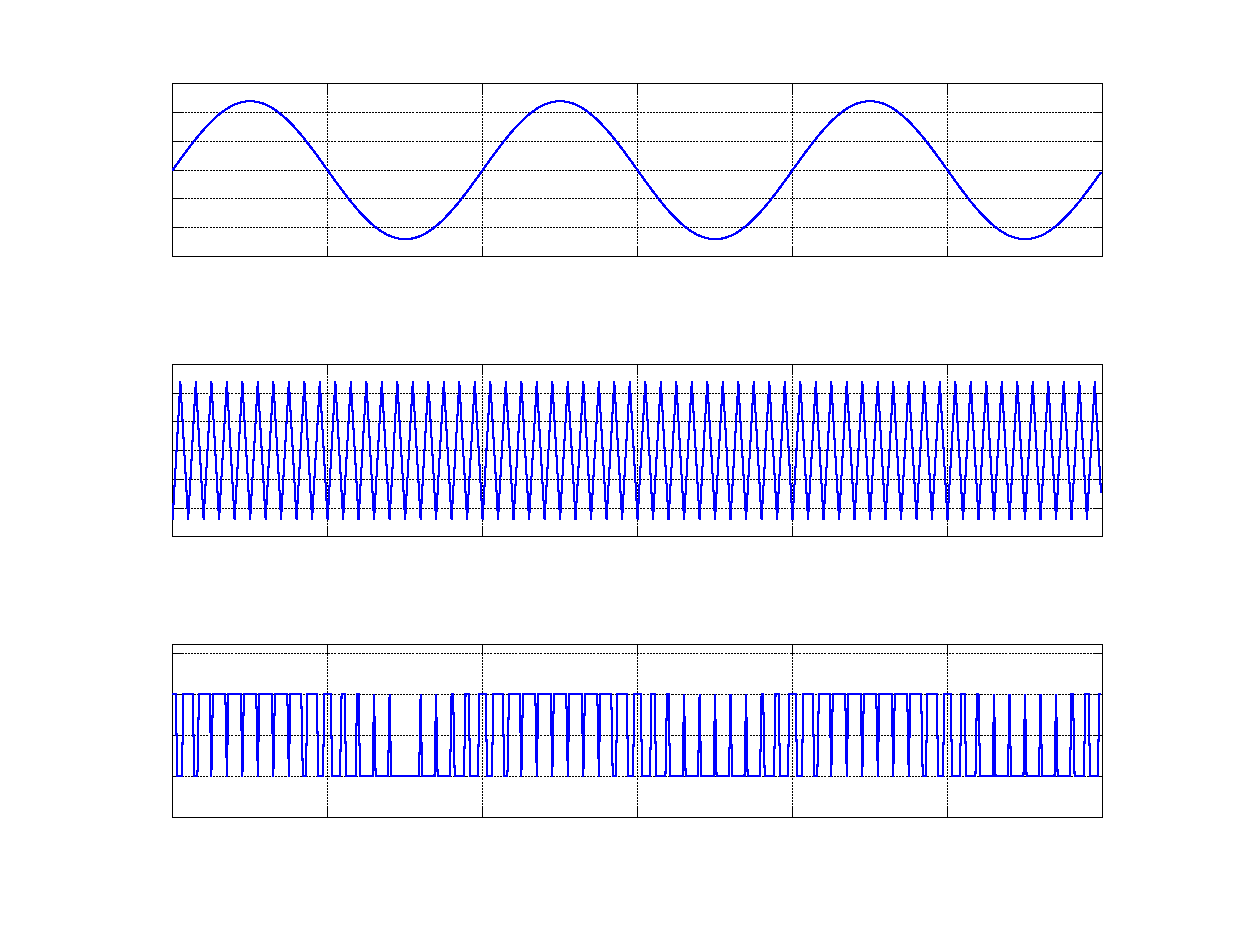
\includegraphics{pwm}}%
    \gplfronttext
  \end{picture}%
\endgroup
$
  %\end{large}}
  %% Creator: Matplotlib, PGF backend
%%
%% To include the figure in your LaTeX document, write
%%   \input{<filename>.pgf}
%%
%% Make sure the required packages are loaded in your preamble
%%   \usepackage{pgf}
%%
%% Figures using additional raster images can only be included by \input if
%% they are in the same directory as the main LaTeX file. For loading figures
%% from other directories you can use the `import` package
%%   \usepackage{import}
%% and then include the figures with
%%   \import{<path to file>}{<filename>.pgf}
%%
%% Matplotlib used the following preamble
%%   \usepackage[utf8x]{inputenc}
%%   \usepackage[T1]{fontenc}
%%
\begingroup%
\makeatletter%
\begin{pgfpicture}%
\pgfpathrectangle{\pgfpointorigin}{\pgfqpoint{5.396430in}{3.335177in}}%
\pgfusepath{use as bounding box, clip}%
\begin{pgfscope}%
\pgfsetbuttcap%
\pgfsetmiterjoin%
\definecolor{currentfill}{rgb}{1.000000,1.000000,1.000000}%
\pgfsetfillcolor{currentfill}%
\pgfsetlinewidth{0.000000pt}%
\definecolor{currentstroke}{rgb}{1.000000,1.000000,1.000000}%
\pgfsetstrokecolor{currentstroke}%
\pgfsetdash{}{0pt}%
\pgfpathmoveto{\pgfqpoint{0.000000in}{0.000000in}}%
\pgfpathlineto{\pgfqpoint{5.396430in}{0.000000in}}%
\pgfpathlineto{\pgfqpoint{5.396430in}{3.335177in}}%
\pgfpathlineto{\pgfqpoint{0.000000in}{3.335177in}}%
\pgfpathclose%
\pgfusepath{fill}%
\end{pgfscope}%
\begin{pgfscope}%
\pgfsetbuttcap%
\pgfsetmiterjoin%
\definecolor{currentfill}{rgb}{1.000000,1.000000,1.000000}%
\pgfsetfillcolor{currentfill}%
\pgfsetlinewidth{0.000000pt}%
\definecolor{currentstroke}{rgb}{0.000000,0.000000,0.000000}%
\pgfsetstrokecolor{currentstroke}%
\pgfsetstrokeopacity{0.000000}%
\pgfsetdash{}{0pt}%
\pgfpathmoveto{\pgfqpoint{0.557102in}{2.631761in}}%
\pgfpathlineto{\pgfqpoint{5.305874in}{2.631761in}}%
\pgfpathlineto{\pgfqpoint{5.305874in}{3.110198in}}%
\pgfpathlineto{\pgfqpoint{0.557102in}{3.110198in}}%
\pgfpathclose%
\pgfusepath{fill}%
\end{pgfscope}%
\begin{pgfscope}%
\pgfpathrectangle{\pgfqpoint{0.557102in}{2.631761in}}{\pgfqpoint{4.748773in}{0.478437in}} %
\pgfusepath{clip}%
\pgfsetbuttcap%
\pgfsetroundjoin%
\pgfsetlinewidth{0.501875pt}%
\definecolor{currentstroke}{rgb}{0.000000,0.000000,0.000000}%
\pgfsetstrokecolor{currentstroke}%
\pgfsetstrokeopacity{0.500000}%
\pgfsetdash{{2.200000pt}{2.200000pt}}{0.000000pt}%
\pgfpathmoveto{\pgfqpoint{0.557102in}{2.631761in}}%
\pgfpathlineto{\pgfqpoint{0.557102in}{3.110198in}}%
\pgfusepath{stroke}%
\end{pgfscope}%
\begin{pgfscope}%
\pgfsetbuttcap%
\pgfsetroundjoin%
\definecolor{currentfill}{rgb}{0.000000,0.000000,0.000000}%
\pgfsetfillcolor{currentfill}%
\pgfsetlinewidth{0.803000pt}%
\definecolor{currentstroke}{rgb}{0.000000,0.000000,0.000000}%
\pgfsetstrokecolor{currentstroke}%
\pgfsetdash{}{0pt}%
\pgfsys@defobject{currentmarker}{\pgfqpoint{0.000000in}{-0.048611in}}{\pgfqpoint{0.000000in}{0.000000in}}{%
\pgfpathmoveto{\pgfqpoint{0.000000in}{0.000000in}}%
\pgfpathlineto{\pgfqpoint{0.000000in}{-0.048611in}}%
\pgfusepath{stroke,fill}%
}%
\begin{pgfscope}%
\pgfsys@transformshift{0.557102in}{2.631761in}%
\pgfsys@useobject{currentmarker}{}%
\end{pgfscope}%
\end{pgfscope}%
\begin{pgfscope}%
\pgftext[x=0.557102in,y=2.534539in,,top]{\rmfamily\fontsize{8.000000}{9.600000}\selectfont \(\displaystyle 0.00\)}%
\end{pgfscope}%
\begin{pgfscope}%
\pgfpathrectangle{\pgfqpoint{0.557102in}{2.631761in}}{\pgfqpoint{4.748773in}{0.478437in}} %
\pgfusepath{clip}%
\pgfsetbuttcap%
\pgfsetroundjoin%
\pgfsetlinewidth{0.501875pt}%
\definecolor{currentstroke}{rgb}{0.000000,0.000000,0.000000}%
\pgfsetstrokecolor{currentstroke}%
\pgfsetstrokeopacity{0.500000}%
\pgfsetdash{{2.200000pt}{2.200000pt}}{0.000000pt}%
\pgfpathmoveto{\pgfqpoint{1.349885in}{2.631761in}}%
\pgfpathlineto{\pgfqpoint{1.349885in}{3.110198in}}%
\pgfusepath{stroke}%
\end{pgfscope}%
\begin{pgfscope}%
\pgfsetbuttcap%
\pgfsetroundjoin%
\definecolor{currentfill}{rgb}{0.000000,0.000000,0.000000}%
\pgfsetfillcolor{currentfill}%
\pgfsetlinewidth{0.803000pt}%
\definecolor{currentstroke}{rgb}{0.000000,0.000000,0.000000}%
\pgfsetstrokecolor{currentstroke}%
\pgfsetdash{}{0pt}%
\pgfsys@defobject{currentmarker}{\pgfqpoint{0.000000in}{-0.048611in}}{\pgfqpoint{0.000000in}{0.000000in}}{%
\pgfpathmoveto{\pgfqpoint{0.000000in}{0.000000in}}%
\pgfpathlineto{\pgfqpoint{0.000000in}{-0.048611in}}%
\pgfusepath{stroke,fill}%
}%
\begin{pgfscope}%
\pgfsys@transformshift{1.349885in}{2.631761in}%
\pgfsys@useobject{currentmarker}{}%
\end{pgfscope}%
\end{pgfscope}%
\begin{pgfscope}%
\pgftext[x=1.349885in,y=2.534539in,,top]{\rmfamily\fontsize{8.000000}{9.600000}\selectfont \(\displaystyle 0.01\)}%
\end{pgfscope}%
\begin{pgfscope}%
\pgfpathrectangle{\pgfqpoint{0.557102in}{2.631761in}}{\pgfqpoint{4.748773in}{0.478437in}} %
\pgfusepath{clip}%
\pgfsetbuttcap%
\pgfsetroundjoin%
\pgfsetlinewidth{0.501875pt}%
\definecolor{currentstroke}{rgb}{0.000000,0.000000,0.000000}%
\pgfsetstrokecolor{currentstroke}%
\pgfsetstrokeopacity{0.500000}%
\pgfsetdash{{2.200000pt}{2.200000pt}}{0.000000pt}%
\pgfpathmoveto{\pgfqpoint{2.142669in}{2.631761in}}%
\pgfpathlineto{\pgfqpoint{2.142669in}{3.110198in}}%
\pgfusepath{stroke}%
\end{pgfscope}%
\begin{pgfscope}%
\pgfsetbuttcap%
\pgfsetroundjoin%
\definecolor{currentfill}{rgb}{0.000000,0.000000,0.000000}%
\pgfsetfillcolor{currentfill}%
\pgfsetlinewidth{0.803000pt}%
\definecolor{currentstroke}{rgb}{0.000000,0.000000,0.000000}%
\pgfsetstrokecolor{currentstroke}%
\pgfsetdash{}{0pt}%
\pgfsys@defobject{currentmarker}{\pgfqpoint{0.000000in}{-0.048611in}}{\pgfqpoint{0.000000in}{0.000000in}}{%
\pgfpathmoveto{\pgfqpoint{0.000000in}{0.000000in}}%
\pgfpathlineto{\pgfqpoint{0.000000in}{-0.048611in}}%
\pgfusepath{stroke,fill}%
}%
\begin{pgfscope}%
\pgfsys@transformshift{2.142669in}{2.631761in}%
\pgfsys@useobject{currentmarker}{}%
\end{pgfscope}%
\end{pgfscope}%
\begin{pgfscope}%
\pgftext[x=2.142669in,y=2.534539in,,top]{\rmfamily\fontsize{8.000000}{9.600000}\selectfont \(\displaystyle 0.02\)}%
\end{pgfscope}%
\begin{pgfscope}%
\pgfpathrectangle{\pgfqpoint{0.557102in}{2.631761in}}{\pgfqpoint{4.748773in}{0.478437in}} %
\pgfusepath{clip}%
\pgfsetbuttcap%
\pgfsetroundjoin%
\pgfsetlinewidth{0.501875pt}%
\definecolor{currentstroke}{rgb}{0.000000,0.000000,0.000000}%
\pgfsetstrokecolor{currentstroke}%
\pgfsetstrokeopacity{0.500000}%
\pgfsetdash{{2.200000pt}{2.200000pt}}{0.000000pt}%
\pgfpathmoveto{\pgfqpoint{2.935452in}{2.631761in}}%
\pgfpathlineto{\pgfqpoint{2.935452in}{3.110198in}}%
\pgfusepath{stroke}%
\end{pgfscope}%
\begin{pgfscope}%
\pgfsetbuttcap%
\pgfsetroundjoin%
\definecolor{currentfill}{rgb}{0.000000,0.000000,0.000000}%
\pgfsetfillcolor{currentfill}%
\pgfsetlinewidth{0.803000pt}%
\definecolor{currentstroke}{rgb}{0.000000,0.000000,0.000000}%
\pgfsetstrokecolor{currentstroke}%
\pgfsetdash{}{0pt}%
\pgfsys@defobject{currentmarker}{\pgfqpoint{0.000000in}{-0.048611in}}{\pgfqpoint{0.000000in}{0.000000in}}{%
\pgfpathmoveto{\pgfqpoint{0.000000in}{0.000000in}}%
\pgfpathlineto{\pgfqpoint{0.000000in}{-0.048611in}}%
\pgfusepath{stroke,fill}%
}%
\begin{pgfscope}%
\pgfsys@transformshift{2.935452in}{2.631761in}%
\pgfsys@useobject{currentmarker}{}%
\end{pgfscope}%
\end{pgfscope}%
\begin{pgfscope}%
\pgftext[x=2.935452in,y=2.534539in,,top]{\rmfamily\fontsize{8.000000}{9.600000}\selectfont \(\displaystyle 0.03\)}%
\end{pgfscope}%
\begin{pgfscope}%
\pgfpathrectangle{\pgfqpoint{0.557102in}{2.631761in}}{\pgfqpoint{4.748773in}{0.478437in}} %
\pgfusepath{clip}%
\pgfsetbuttcap%
\pgfsetroundjoin%
\pgfsetlinewidth{0.501875pt}%
\definecolor{currentstroke}{rgb}{0.000000,0.000000,0.000000}%
\pgfsetstrokecolor{currentstroke}%
\pgfsetstrokeopacity{0.500000}%
\pgfsetdash{{2.200000pt}{2.200000pt}}{0.000000pt}%
\pgfpathmoveto{\pgfqpoint{3.728235in}{2.631761in}}%
\pgfpathlineto{\pgfqpoint{3.728235in}{3.110198in}}%
\pgfusepath{stroke}%
\end{pgfscope}%
\begin{pgfscope}%
\pgfsetbuttcap%
\pgfsetroundjoin%
\definecolor{currentfill}{rgb}{0.000000,0.000000,0.000000}%
\pgfsetfillcolor{currentfill}%
\pgfsetlinewidth{0.803000pt}%
\definecolor{currentstroke}{rgb}{0.000000,0.000000,0.000000}%
\pgfsetstrokecolor{currentstroke}%
\pgfsetdash{}{0pt}%
\pgfsys@defobject{currentmarker}{\pgfqpoint{0.000000in}{-0.048611in}}{\pgfqpoint{0.000000in}{0.000000in}}{%
\pgfpathmoveto{\pgfqpoint{0.000000in}{0.000000in}}%
\pgfpathlineto{\pgfqpoint{0.000000in}{-0.048611in}}%
\pgfusepath{stroke,fill}%
}%
\begin{pgfscope}%
\pgfsys@transformshift{3.728235in}{2.631761in}%
\pgfsys@useobject{currentmarker}{}%
\end{pgfscope}%
\end{pgfscope}%
\begin{pgfscope}%
\pgftext[x=3.728235in,y=2.534539in,,top]{\rmfamily\fontsize{8.000000}{9.600000}\selectfont \(\displaystyle 0.04\)}%
\end{pgfscope}%
\begin{pgfscope}%
\pgfpathrectangle{\pgfqpoint{0.557102in}{2.631761in}}{\pgfqpoint{4.748773in}{0.478437in}} %
\pgfusepath{clip}%
\pgfsetbuttcap%
\pgfsetroundjoin%
\pgfsetlinewidth{0.501875pt}%
\definecolor{currentstroke}{rgb}{0.000000,0.000000,0.000000}%
\pgfsetstrokecolor{currentstroke}%
\pgfsetstrokeopacity{0.500000}%
\pgfsetdash{{2.200000pt}{2.200000pt}}{0.000000pt}%
\pgfpathmoveto{\pgfqpoint{4.521019in}{2.631761in}}%
\pgfpathlineto{\pgfqpoint{4.521019in}{3.110198in}}%
\pgfusepath{stroke}%
\end{pgfscope}%
\begin{pgfscope}%
\pgfsetbuttcap%
\pgfsetroundjoin%
\definecolor{currentfill}{rgb}{0.000000,0.000000,0.000000}%
\pgfsetfillcolor{currentfill}%
\pgfsetlinewidth{0.803000pt}%
\definecolor{currentstroke}{rgb}{0.000000,0.000000,0.000000}%
\pgfsetstrokecolor{currentstroke}%
\pgfsetdash{}{0pt}%
\pgfsys@defobject{currentmarker}{\pgfqpoint{0.000000in}{-0.048611in}}{\pgfqpoint{0.000000in}{0.000000in}}{%
\pgfpathmoveto{\pgfqpoint{0.000000in}{0.000000in}}%
\pgfpathlineto{\pgfqpoint{0.000000in}{-0.048611in}}%
\pgfusepath{stroke,fill}%
}%
\begin{pgfscope}%
\pgfsys@transformshift{4.521019in}{2.631761in}%
\pgfsys@useobject{currentmarker}{}%
\end{pgfscope}%
\end{pgfscope}%
\begin{pgfscope}%
\pgftext[x=4.521019in,y=2.534539in,,top]{\rmfamily\fontsize{8.000000}{9.600000}\selectfont \(\displaystyle 0.05\)}%
\end{pgfscope}%
\begin{pgfscope}%
\pgftext[x=2.931488in,y=2.380859in,,top]{\rmfamily\fontsize{10.000000}{12.000000}\selectfont \(\displaystyle t/s\)}%
\end{pgfscope}%
\begin{pgfscope}%
\pgfpathrectangle{\pgfqpoint{0.557102in}{2.631761in}}{\pgfqpoint{4.748773in}{0.478437in}} %
\pgfusepath{clip}%
\pgfsetbuttcap%
\pgfsetroundjoin%
\pgfsetlinewidth{0.501875pt}%
\definecolor{currentstroke}{rgb}{0.000000,0.000000,0.000000}%
\pgfsetstrokecolor{currentstroke}%
\pgfsetstrokeopacity{0.500000}%
\pgfsetdash{{2.200000pt}{2.200000pt}}{0.000000pt}%
\pgfpathmoveto{\pgfqpoint{0.557102in}{2.711500in}}%
\pgfpathlineto{\pgfqpoint{5.305874in}{2.711500in}}%
\pgfusepath{stroke}%
\end{pgfscope}%
\begin{pgfscope}%
\pgfsetbuttcap%
\pgfsetroundjoin%
\definecolor{currentfill}{rgb}{0.000000,0.000000,0.000000}%
\pgfsetfillcolor{currentfill}%
\pgfsetlinewidth{0.803000pt}%
\definecolor{currentstroke}{rgb}{0.000000,0.000000,0.000000}%
\pgfsetstrokecolor{currentstroke}%
\pgfsetdash{}{0pt}%
\pgfsys@defobject{currentmarker}{\pgfqpoint{-0.048611in}{0.000000in}}{\pgfqpoint{0.000000in}{0.000000in}}{%
\pgfpathmoveto{\pgfqpoint{0.000000in}{0.000000in}}%
\pgfpathlineto{\pgfqpoint{-0.048611in}{0.000000in}}%
\pgfusepath{stroke,fill}%
}%
\begin{pgfscope}%
\pgfsys@transformshift{0.557102in}{2.711500in}%
\pgfsys@useobject{currentmarker}{}%
\end{pgfscope}%
\end{pgfscope}%
\begin{pgfscope}%
\pgftext[x=0.250000in,y=2.673238in,left,base]{\rmfamily\fontsize{8.000000}{9.600000}\selectfont \(\displaystyle -10\)}%
\end{pgfscope}%
\begin{pgfscope}%
\pgfpathrectangle{\pgfqpoint{0.557102in}{2.631761in}}{\pgfqpoint{4.748773in}{0.478437in}} %
\pgfusepath{clip}%
\pgfsetbuttcap%
\pgfsetroundjoin%
\pgfsetlinewidth{0.501875pt}%
\definecolor{currentstroke}{rgb}{0.000000,0.000000,0.000000}%
\pgfsetstrokecolor{currentstroke}%
\pgfsetstrokeopacity{0.500000}%
\pgfsetdash{{2.200000pt}{2.200000pt}}{0.000000pt}%
\pgfpathmoveto{\pgfqpoint{0.557102in}{2.870980in}}%
\pgfpathlineto{\pgfqpoint{5.305874in}{2.870980in}}%
\pgfusepath{stroke}%
\end{pgfscope}%
\begin{pgfscope}%
\pgfsetbuttcap%
\pgfsetroundjoin%
\definecolor{currentfill}{rgb}{0.000000,0.000000,0.000000}%
\pgfsetfillcolor{currentfill}%
\pgfsetlinewidth{0.803000pt}%
\definecolor{currentstroke}{rgb}{0.000000,0.000000,0.000000}%
\pgfsetstrokecolor{currentstroke}%
\pgfsetdash{}{0pt}%
\pgfsys@defobject{currentmarker}{\pgfqpoint{-0.048611in}{0.000000in}}{\pgfqpoint{0.000000in}{0.000000in}}{%
\pgfpathmoveto{\pgfqpoint{0.000000in}{0.000000in}}%
\pgfpathlineto{\pgfqpoint{-0.048611in}{0.000000in}}%
\pgfusepath{stroke,fill}%
}%
\begin{pgfscope}%
\pgfsys@transformshift{0.557102in}{2.870980in}%
\pgfsys@useobject{currentmarker}{}%
\end{pgfscope}%
\end{pgfscope}%
\begin{pgfscope}%
\pgftext[x=0.400851in,y=2.832717in,left,base]{\rmfamily\fontsize{8.000000}{9.600000}\selectfont \(\displaystyle 0\)}%
\end{pgfscope}%
\begin{pgfscope}%
\pgfpathrectangle{\pgfqpoint{0.557102in}{2.631761in}}{\pgfqpoint{4.748773in}{0.478437in}} %
\pgfusepath{clip}%
\pgfsetbuttcap%
\pgfsetroundjoin%
\pgfsetlinewidth{0.501875pt}%
\definecolor{currentstroke}{rgb}{0.000000,0.000000,0.000000}%
\pgfsetstrokecolor{currentstroke}%
\pgfsetstrokeopacity{0.500000}%
\pgfsetdash{{2.200000pt}{2.200000pt}}{0.000000pt}%
\pgfpathmoveto{\pgfqpoint{0.557102in}{3.030459in}}%
\pgfpathlineto{\pgfqpoint{5.305874in}{3.030459in}}%
\pgfusepath{stroke}%
\end{pgfscope}%
\begin{pgfscope}%
\pgfsetbuttcap%
\pgfsetroundjoin%
\definecolor{currentfill}{rgb}{0.000000,0.000000,0.000000}%
\pgfsetfillcolor{currentfill}%
\pgfsetlinewidth{0.803000pt}%
\definecolor{currentstroke}{rgb}{0.000000,0.000000,0.000000}%
\pgfsetstrokecolor{currentstroke}%
\pgfsetdash{}{0pt}%
\pgfsys@defobject{currentmarker}{\pgfqpoint{-0.048611in}{0.000000in}}{\pgfqpoint{0.000000in}{0.000000in}}{%
\pgfpathmoveto{\pgfqpoint{0.000000in}{0.000000in}}%
\pgfpathlineto{\pgfqpoint{-0.048611in}{0.000000in}}%
\pgfusepath{stroke,fill}%
}%
\begin{pgfscope}%
\pgfsys@transformshift{0.557102in}{3.030459in}%
\pgfsys@useobject{currentmarker}{}%
\end{pgfscope}%
\end{pgfscope}%
\begin{pgfscope}%
\pgftext[x=0.341822in,y=2.992196in,left,base]{\rmfamily\fontsize{8.000000}{9.600000}\selectfont \(\displaystyle 10\)}%
\end{pgfscope}%
\begin{pgfscope}%
\pgftext[x=0.194444in,y=2.870980in,,bottom,rotate=90.000000]{\rmfamily\fontsize{10.000000}{12.000000}\selectfont \(\displaystyle u_{m}/V\)}%
\end{pgfscope}%
\begin{pgfscope}%
\pgfpathrectangle{\pgfqpoint{0.557102in}{2.631761in}}{\pgfqpoint{4.748773in}{0.478437in}} %
\pgfusepath{clip}%
\pgfsetrectcap%
\pgfsetroundjoin%
\pgfsetlinewidth{0.752812pt}%
\definecolor{currentstroke}{rgb}{0.121569,0.466667,0.705882}%
\pgfsetstrokecolor{currentstroke}%
\pgfsetdash{}{0pt}%
\pgfpathmoveto{\pgfqpoint{0.557102in}{2.870980in}}%
\pgfpathlineto{\pgfqpoint{0.644308in}{2.935805in}}%
\pgfpathlineto{\pgfqpoint{0.691875in}{2.968397in}}%
\pgfpathlineto{\pgfqpoint{0.731514in}{2.992967in}}%
\pgfpathlineto{\pgfqpoint{0.763225in}{3.010486in}}%
\pgfpathlineto{\pgfqpoint{0.794937in}{3.025805in}}%
\pgfpathlineto{\pgfqpoint{0.826648in}{3.038683in}}%
\pgfpathlineto{\pgfqpoint{0.858360in}{3.048915in}}%
\pgfpathlineto{\pgfqpoint{0.890071in}{3.056342in}}%
\pgfpathlineto{\pgfqpoint{0.921782in}{3.060845in}}%
\pgfpathlineto{\pgfqpoint{0.945566in}{3.062260in}}%
\pgfpathlineto{\pgfqpoint{0.969349in}{3.061977in}}%
\pgfpathlineto{\pgfqpoint{0.993133in}{3.059998in}}%
\pgfpathlineto{\pgfqpoint{1.024844in}{3.054756in}}%
\pgfpathlineto{\pgfqpoint{1.056555in}{3.046615in}}%
\pgfpathlineto{\pgfqpoint{1.088267in}{3.035704in}}%
\pgfpathlineto{\pgfqpoint{1.119978in}{3.022195in}}%
\pgfpathlineto{\pgfqpoint{1.151689in}{3.006302in}}%
\pgfpathlineto{\pgfqpoint{1.191329in}{2.983467in}}%
\pgfpathlineto{\pgfqpoint{1.230968in}{2.957862in}}%
\pgfpathlineto{\pgfqpoint{1.278535in}{2.924371in}}%
\pgfpathlineto{\pgfqpoint{1.349885in}{2.870980in}}%
\pgfpathlineto{\pgfqpoint{1.437091in}{2.806154in}}%
\pgfpathlineto{\pgfqpoint{1.484658in}{2.773562in}}%
\pgfpathlineto{\pgfqpoint{1.524298in}{2.748993in}}%
\pgfpathlineto{\pgfqpoint{1.556009in}{2.731473in}}%
\pgfpathlineto{\pgfqpoint{1.587720in}{2.716154in}}%
\pgfpathlineto{\pgfqpoint{1.619432in}{2.703276in}}%
\pgfpathlineto{\pgfqpoint{1.651143in}{2.693044in}}%
\pgfpathlineto{\pgfqpoint{1.682854in}{2.685617in}}%
\pgfpathlineto{\pgfqpoint{1.714566in}{2.681114in}}%
\pgfpathlineto{\pgfqpoint{1.738349in}{2.679699in}}%
\pgfpathlineto{\pgfqpoint{1.762133in}{2.679982in}}%
\pgfpathlineto{\pgfqpoint{1.785916in}{2.681961in}}%
\pgfpathlineto{\pgfqpoint{1.817627in}{2.687203in}}%
\pgfpathlineto{\pgfqpoint{1.849339in}{2.695344in}}%
\pgfpathlineto{\pgfqpoint{1.881050in}{2.706255in}}%
\pgfpathlineto{\pgfqpoint{1.912761in}{2.719764in}}%
\pgfpathlineto{\pgfqpoint{1.944473in}{2.735657in}}%
\pgfpathlineto{\pgfqpoint{1.984112in}{2.758492in}}%
\pgfpathlineto{\pgfqpoint{2.023751in}{2.784097in}}%
\pgfpathlineto{\pgfqpoint{2.071318in}{2.817588in}}%
\pgfpathlineto{\pgfqpoint{2.142669in}{2.870980in}}%
\pgfpathlineto{\pgfqpoint{2.229875in}{2.935805in}}%
\pgfpathlineto{\pgfqpoint{2.277442in}{2.968397in}}%
\pgfpathlineto{\pgfqpoint{2.317081in}{2.992967in}}%
\pgfpathlineto{\pgfqpoint{2.348792in}{3.010486in}}%
\pgfpathlineto{\pgfqpoint{2.380504in}{3.025805in}}%
\pgfpathlineto{\pgfqpoint{2.412215in}{3.038683in}}%
\pgfpathlineto{\pgfqpoint{2.443926in}{3.048915in}}%
\pgfpathlineto{\pgfqpoint{2.475638in}{3.056342in}}%
\pgfpathlineto{\pgfqpoint{2.507349in}{3.060845in}}%
\pgfpathlineto{\pgfqpoint{2.531133in}{3.062260in}}%
\pgfpathlineto{\pgfqpoint{2.554916in}{3.061977in}}%
\pgfpathlineto{\pgfqpoint{2.578700in}{3.059998in}}%
\pgfpathlineto{\pgfqpoint{2.610411in}{3.054756in}}%
\pgfpathlineto{\pgfqpoint{2.642122in}{3.046615in}}%
\pgfpathlineto{\pgfqpoint{2.673834in}{3.035704in}}%
\pgfpathlineto{\pgfqpoint{2.705545in}{3.022195in}}%
\pgfpathlineto{\pgfqpoint{2.737256in}{3.006302in}}%
\pgfpathlineto{\pgfqpoint{2.776895in}{2.983467in}}%
\pgfpathlineto{\pgfqpoint{2.816535in}{2.957862in}}%
\pgfpathlineto{\pgfqpoint{2.864102in}{2.924371in}}%
\pgfpathlineto{\pgfqpoint{2.935452in}{2.870980in}}%
\pgfpathlineto{\pgfqpoint{3.022658in}{2.806154in}}%
\pgfpathlineto{\pgfqpoint{3.070225in}{2.773562in}}%
\pgfpathlineto{\pgfqpoint{3.109864in}{2.748993in}}%
\pgfpathlineto{\pgfqpoint{3.141576in}{2.731473in}}%
\pgfpathlineto{\pgfqpoint{3.173287in}{2.716154in}}%
\pgfpathlineto{\pgfqpoint{3.204998in}{2.703276in}}%
\pgfpathlineto{\pgfqpoint{3.236710in}{2.693044in}}%
\pgfpathlineto{\pgfqpoint{3.268421in}{2.685617in}}%
\pgfpathlineto{\pgfqpoint{3.300132in}{2.681114in}}%
\pgfpathlineto{\pgfqpoint{3.323916in}{2.679699in}}%
\pgfpathlineto{\pgfqpoint{3.347699in}{2.679982in}}%
\pgfpathlineto{\pgfqpoint{3.371483in}{2.681961in}}%
\pgfpathlineto{\pgfqpoint{3.403194in}{2.687203in}}%
\pgfpathlineto{\pgfqpoint{3.434906in}{2.695344in}}%
\pgfpathlineto{\pgfqpoint{3.466617in}{2.706255in}}%
\pgfpathlineto{\pgfqpoint{3.498328in}{2.719764in}}%
\pgfpathlineto{\pgfqpoint{3.530040in}{2.735657in}}%
\pgfpathlineto{\pgfqpoint{3.569679in}{2.758492in}}%
\pgfpathlineto{\pgfqpoint{3.609318in}{2.784097in}}%
\pgfpathlineto{\pgfqpoint{3.656885in}{2.817588in}}%
\pgfpathlineto{\pgfqpoint{3.728235in}{2.870980in}}%
\pgfpathlineto{\pgfqpoint{3.815442in}{2.935805in}}%
\pgfpathlineto{\pgfqpoint{3.863009in}{2.968397in}}%
\pgfpathlineto{\pgfqpoint{3.902648in}{2.992967in}}%
\pgfpathlineto{\pgfqpoint{3.934359in}{3.010486in}}%
\pgfpathlineto{\pgfqpoint{3.966071in}{3.025805in}}%
\pgfpathlineto{\pgfqpoint{3.997782in}{3.038683in}}%
\pgfpathlineto{\pgfqpoint{4.029493in}{3.048915in}}%
\pgfpathlineto{\pgfqpoint{4.061205in}{3.056342in}}%
\pgfpathlineto{\pgfqpoint{4.092916in}{3.060845in}}%
\pgfpathlineto{\pgfqpoint{4.116699in}{3.062260in}}%
\pgfpathlineto{\pgfqpoint{4.140483in}{3.061977in}}%
\pgfpathlineto{\pgfqpoint{4.164266in}{3.059998in}}%
\pgfpathlineto{\pgfqpoint{4.195978in}{3.054756in}}%
\pgfpathlineto{\pgfqpoint{4.227689in}{3.046615in}}%
\pgfpathlineto{\pgfqpoint{4.259400in}{3.035704in}}%
\pgfpathlineto{\pgfqpoint{4.291112in}{3.022195in}}%
\pgfpathlineto{\pgfqpoint{4.322823in}{3.006302in}}%
\pgfpathlineto{\pgfqpoint{4.362462in}{2.983467in}}%
\pgfpathlineto{\pgfqpoint{4.402101in}{2.957862in}}%
\pgfpathlineto{\pgfqpoint{4.449668in}{2.924371in}}%
\pgfpathlineto{\pgfqpoint{4.521019in}{2.870980in}}%
\pgfpathlineto{\pgfqpoint{4.608225in}{2.806154in}}%
\pgfpathlineto{\pgfqpoint{4.655792in}{2.773562in}}%
\pgfpathlineto{\pgfqpoint{4.695431in}{2.748993in}}%
\pgfpathlineto{\pgfqpoint{4.727143in}{2.731473in}}%
\pgfpathlineto{\pgfqpoint{4.758854in}{2.716154in}}%
\pgfpathlineto{\pgfqpoint{4.790565in}{2.703276in}}%
\pgfpathlineto{\pgfqpoint{4.822277in}{2.693044in}}%
\pgfpathlineto{\pgfqpoint{4.853988in}{2.685617in}}%
\pgfpathlineto{\pgfqpoint{4.885699in}{2.681114in}}%
\pgfpathlineto{\pgfqpoint{4.909483in}{2.679699in}}%
\pgfpathlineto{\pgfqpoint{4.933266in}{2.679982in}}%
\pgfpathlineto{\pgfqpoint{4.957050in}{2.681961in}}%
\pgfpathlineto{\pgfqpoint{4.988761in}{2.687203in}}%
\pgfpathlineto{\pgfqpoint{5.020472in}{2.695344in}}%
\pgfpathlineto{\pgfqpoint{5.052184in}{2.706255in}}%
\pgfpathlineto{\pgfqpoint{5.083895in}{2.719764in}}%
\pgfpathlineto{\pgfqpoint{5.115606in}{2.735657in}}%
\pgfpathlineto{\pgfqpoint{5.155246in}{2.758492in}}%
\pgfpathlineto{\pgfqpoint{5.194885in}{2.784097in}}%
\pgfpathlineto{\pgfqpoint{5.242452in}{2.817588in}}%
\pgfpathlineto{\pgfqpoint{5.305874in}{2.864968in}}%
\pgfpathlineto{\pgfqpoint{5.305874in}{2.864968in}}%
\pgfusepath{stroke}%
\end{pgfscope}%
\begin{pgfscope}%
\pgfsetrectcap%
\pgfsetmiterjoin%
\pgfsetlinewidth{0.501875pt}%
\definecolor{currentstroke}{rgb}{0.000000,0.000000,0.000000}%
\pgfsetstrokecolor{currentstroke}%
\pgfsetdash{}{0pt}%
\pgfpathmoveto{\pgfqpoint{0.557102in}{2.631761in}}%
\pgfpathlineto{\pgfqpoint{0.557102in}{3.110198in}}%
\pgfusepath{stroke}%
\end{pgfscope}%
\begin{pgfscope}%
\pgfsetrectcap%
\pgfsetmiterjoin%
\pgfsetlinewidth{0.501875pt}%
\definecolor{currentstroke}{rgb}{0.000000,0.000000,0.000000}%
\pgfsetstrokecolor{currentstroke}%
\pgfsetdash{}{0pt}%
\pgfpathmoveto{\pgfqpoint{5.305874in}{2.631761in}}%
\pgfpathlineto{\pgfqpoint{5.305874in}{3.110198in}}%
\pgfusepath{stroke}%
\end{pgfscope}%
\begin{pgfscope}%
\pgfsetrectcap%
\pgfsetmiterjoin%
\pgfsetlinewidth{0.501875pt}%
\definecolor{currentstroke}{rgb}{0.000000,0.000000,0.000000}%
\pgfsetstrokecolor{currentstroke}%
\pgfsetdash{}{0pt}%
\pgfpathmoveto{\pgfqpoint{0.557102in}{2.631761in}}%
\pgfpathlineto{\pgfqpoint{5.305874in}{2.631761in}}%
\pgfusepath{stroke}%
\end{pgfscope}%
\begin{pgfscope}%
\pgfsetrectcap%
\pgfsetmiterjoin%
\pgfsetlinewidth{0.501875pt}%
\definecolor{currentstroke}{rgb}{0.000000,0.000000,0.000000}%
\pgfsetstrokecolor{currentstroke}%
\pgfsetdash{}{0pt}%
\pgfpathmoveto{\pgfqpoint{0.557102in}{3.110198in}}%
\pgfpathlineto{\pgfqpoint{5.305874in}{3.110198in}}%
\pgfusepath{stroke}%
\end{pgfscope}%
\begin{pgfscope}%
\pgftext[x=2.931488in,y=3.193531in,,base]{\rmfamily\fontsize{9.000000}{10.800000}\selectfont Nachrichtensignal}%
\end{pgfscope}%
\begin{pgfscope}%
\pgfsetbuttcap%
\pgfsetmiterjoin%
\definecolor{currentfill}{rgb}{1.000000,1.000000,1.000000}%
\pgfsetfillcolor{currentfill}%
\pgfsetlinewidth{0.000000pt}%
\definecolor{currentstroke}{rgb}{0.000000,0.000000,0.000000}%
\pgfsetstrokecolor{currentstroke}%
\pgfsetstrokeopacity{0.000000}%
\pgfsetdash{}{0pt}%
\pgfpathmoveto{\pgfqpoint{0.557102in}{1.538554in}}%
\pgfpathlineto{\pgfqpoint{5.305874in}{1.538554in}}%
\pgfpathlineto{\pgfqpoint{5.305874in}{2.016991in}}%
\pgfpathlineto{\pgfqpoint{0.557102in}{2.016991in}}%
\pgfpathclose%
\pgfusepath{fill}%
\end{pgfscope}%
\begin{pgfscope}%
\pgfpathrectangle{\pgfqpoint{0.557102in}{1.538554in}}{\pgfqpoint{4.748773in}{0.478437in}} %
\pgfusepath{clip}%
\pgfsetbuttcap%
\pgfsetroundjoin%
\pgfsetlinewidth{0.501875pt}%
\definecolor{currentstroke}{rgb}{0.000000,0.000000,0.000000}%
\pgfsetstrokecolor{currentstroke}%
\pgfsetstrokeopacity{0.500000}%
\pgfsetdash{{2.200000pt}{2.200000pt}}{0.000000pt}%
\pgfpathmoveto{\pgfqpoint{0.557102in}{1.538554in}}%
\pgfpathlineto{\pgfqpoint{0.557102in}{2.016991in}}%
\pgfusepath{stroke}%
\end{pgfscope}%
\begin{pgfscope}%
\pgfsetbuttcap%
\pgfsetroundjoin%
\definecolor{currentfill}{rgb}{0.000000,0.000000,0.000000}%
\pgfsetfillcolor{currentfill}%
\pgfsetlinewidth{0.803000pt}%
\definecolor{currentstroke}{rgb}{0.000000,0.000000,0.000000}%
\pgfsetstrokecolor{currentstroke}%
\pgfsetdash{}{0pt}%
\pgfsys@defobject{currentmarker}{\pgfqpoint{0.000000in}{-0.048611in}}{\pgfqpoint{0.000000in}{0.000000in}}{%
\pgfpathmoveto{\pgfqpoint{0.000000in}{0.000000in}}%
\pgfpathlineto{\pgfqpoint{0.000000in}{-0.048611in}}%
\pgfusepath{stroke,fill}%
}%
\begin{pgfscope}%
\pgfsys@transformshift{0.557102in}{1.538554in}%
\pgfsys@useobject{currentmarker}{}%
\end{pgfscope}%
\end{pgfscope}%
\begin{pgfscope}%
\pgftext[x=0.557102in,y=1.441332in,,top]{\rmfamily\fontsize{8.000000}{9.600000}\selectfont \(\displaystyle 0.00\)}%
\end{pgfscope}%
\begin{pgfscope}%
\pgfpathrectangle{\pgfqpoint{0.557102in}{1.538554in}}{\pgfqpoint{4.748773in}{0.478437in}} %
\pgfusepath{clip}%
\pgfsetbuttcap%
\pgfsetroundjoin%
\pgfsetlinewidth{0.501875pt}%
\definecolor{currentstroke}{rgb}{0.000000,0.000000,0.000000}%
\pgfsetstrokecolor{currentstroke}%
\pgfsetstrokeopacity{0.500000}%
\pgfsetdash{{2.200000pt}{2.200000pt}}{0.000000pt}%
\pgfpathmoveto{\pgfqpoint{1.349885in}{1.538554in}}%
\pgfpathlineto{\pgfqpoint{1.349885in}{2.016991in}}%
\pgfusepath{stroke}%
\end{pgfscope}%
\begin{pgfscope}%
\pgfsetbuttcap%
\pgfsetroundjoin%
\definecolor{currentfill}{rgb}{0.000000,0.000000,0.000000}%
\pgfsetfillcolor{currentfill}%
\pgfsetlinewidth{0.803000pt}%
\definecolor{currentstroke}{rgb}{0.000000,0.000000,0.000000}%
\pgfsetstrokecolor{currentstroke}%
\pgfsetdash{}{0pt}%
\pgfsys@defobject{currentmarker}{\pgfqpoint{0.000000in}{-0.048611in}}{\pgfqpoint{0.000000in}{0.000000in}}{%
\pgfpathmoveto{\pgfqpoint{0.000000in}{0.000000in}}%
\pgfpathlineto{\pgfqpoint{0.000000in}{-0.048611in}}%
\pgfusepath{stroke,fill}%
}%
\begin{pgfscope}%
\pgfsys@transformshift{1.349885in}{1.538554in}%
\pgfsys@useobject{currentmarker}{}%
\end{pgfscope}%
\end{pgfscope}%
\begin{pgfscope}%
\pgftext[x=1.349885in,y=1.441332in,,top]{\rmfamily\fontsize{8.000000}{9.600000}\selectfont \(\displaystyle 0.01\)}%
\end{pgfscope}%
\begin{pgfscope}%
\pgfpathrectangle{\pgfqpoint{0.557102in}{1.538554in}}{\pgfqpoint{4.748773in}{0.478437in}} %
\pgfusepath{clip}%
\pgfsetbuttcap%
\pgfsetroundjoin%
\pgfsetlinewidth{0.501875pt}%
\definecolor{currentstroke}{rgb}{0.000000,0.000000,0.000000}%
\pgfsetstrokecolor{currentstroke}%
\pgfsetstrokeopacity{0.500000}%
\pgfsetdash{{2.200000pt}{2.200000pt}}{0.000000pt}%
\pgfpathmoveto{\pgfqpoint{2.142669in}{1.538554in}}%
\pgfpathlineto{\pgfqpoint{2.142669in}{2.016991in}}%
\pgfusepath{stroke}%
\end{pgfscope}%
\begin{pgfscope}%
\pgfsetbuttcap%
\pgfsetroundjoin%
\definecolor{currentfill}{rgb}{0.000000,0.000000,0.000000}%
\pgfsetfillcolor{currentfill}%
\pgfsetlinewidth{0.803000pt}%
\definecolor{currentstroke}{rgb}{0.000000,0.000000,0.000000}%
\pgfsetstrokecolor{currentstroke}%
\pgfsetdash{}{0pt}%
\pgfsys@defobject{currentmarker}{\pgfqpoint{0.000000in}{-0.048611in}}{\pgfqpoint{0.000000in}{0.000000in}}{%
\pgfpathmoveto{\pgfqpoint{0.000000in}{0.000000in}}%
\pgfpathlineto{\pgfqpoint{0.000000in}{-0.048611in}}%
\pgfusepath{stroke,fill}%
}%
\begin{pgfscope}%
\pgfsys@transformshift{2.142669in}{1.538554in}%
\pgfsys@useobject{currentmarker}{}%
\end{pgfscope}%
\end{pgfscope}%
\begin{pgfscope}%
\pgftext[x=2.142669in,y=1.441332in,,top]{\rmfamily\fontsize{8.000000}{9.600000}\selectfont \(\displaystyle 0.02\)}%
\end{pgfscope}%
\begin{pgfscope}%
\pgfpathrectangle{\pgfqpoint{0.557102in}{1.538554in}}{\pgfqpoint{4.748773in}{0.478437in}} %
\pgfusepath{clip}%
\pgfsetbuttcap%
\pgfsetroundjoin%
\pgfsetlinewidth{0.501875pt}%
\definecolor{currentstroke}{rgb}{0.000000,0.000000,0.000000}%
\pgfsetstrokecolor{currentstroke}%
\pgfsetstrokeopacity{0.500000}%
\pgfsetdash{{2.200000pt}{2.200000pt}}{0.000000pt}%
\pgfpathmoveto{\pgfqpoint{2.935452in}{1.538554in}}%
\pgfpathlineto{\pgfqpoint{2.935452in}{2.016991in}}%
\pgfusepath{stroke}%
\end{pgfscope}%
\begin{pgfscope}%
\pgfsetbuttcap%
\pgfsetroundjoin%
\definecolor{currentfill}{rgb}{0.000000,0.000000,0.000000}%
\pgfsetfillcolor{currentfill}%
\pgfsetlinewidth{0.803000pt}%
\definecolor{currentstroke}{rgb}{0.000000,0.000000,0.000000}%
\pgfsetstrokecolor{currentstroke}%
\pgfsetdash{}{0pt}%
\pgfsys@defobject{currentmarker}{\pgfqpoint{0.000000in}{-0.048611in}}{\pgfqpoint{0.000000in}{0.000000in}}{%
\pgfpathmoveto{\pgfqpoint{0.000000in}{0.000000in}}%
\pgfpathlineto{\pgfqpoint{0.000000in}{-0.048611in}}%
\pgfusepath{stroke,fill}%
}%
\begin{pgfscope}%
\pgfsys@transformshift{2.935452in}{1.538554in}%
\pgfsys@useobject{currentmarker}{}%
\end{pgfscope}%
\end{pgfscope}%
\begin{pgfscope}%
\pgftext[x=2.935452in,y=1.441332in,,top]{\rmfamily\fontsize{8.000000}{9.600000}\selectfont \(\displaystyle 0.03\)}%
\end{pgfscope}%
\begin{pgfscope}%
\pgfpathrectangle{\pgfqpoint{0.557102in}{1.538554in}}{\pgfqpoint{4.748773in}{0.478437in}} %
\pgfusepath{clip}%
\pgfsetbuttcap%
\pgfsetroundjoin%
\pgfsetlinewidth{0.501875pt}%
\definecolor{currentstroke}{rgb}{0.000000,0.000000,0.000000}%
\pgfsetstrokecolor{currentstroke}%
\pgfsetstrokeopacity{0.500000}%
\pgfsetdash{{2.200000pt}{2.200000pt}}{0.000000pt}%
\pgfpathmoveto{\pgfqpoint{3.728235in}{1.538554in}}%
\pgfpathlineto{\pgfqpoint{3.728235in}{2.016991in}}%
\pgfusepath{stroke}%
\end{pgfscope}%
\begin{pgfscope}%
\pgfsetbuttcap%
\pgfsetroundjoin%
\definecolor{currentfill}{rgb}{0.000000,0.000000,0.000000}%
\pgfsetfillcolor{currentfill}%
\pgfsetlinewidth{0.803000pt}%
\definecolor{currentstroke}{rgb}{0.000000,0.000000,0.000000}%
\pgfsetstrokecolor{currentstroke}%
\pgfsetdash{}{0pt}%
\pgfsys@defobject{currentmarker}{\pgfqpoint{0.000000in}{-0.048611in}}{\pgfqpoint{0.000000in}{0.000000in}}{%
\pgfpathmoveto{\pgfqpoint{0.000000in}{0.000000in}}%
\pgfpathlineto{\pgfqpoint{0.000000in}{-0.048611in}}%
\pgfusepath{stroke,fill}%
}%
\begin{pgfscope}%
\pgfsys@transformshift{3.728235in}{1.538554in}%
\pgfsys@useobject{currentmarker}{}%
\end{pgfscope}%
\end{pgfscope}%
\begin{pgfscope}%
\pgftext[x=3.728235in,y=1.441332in,,top]{\rmfamily\fontsize{8.000000}{9.600000}\selectfont \(\displaystyle 0.04\)}%
\end{pgfscope}%
\begin{pgfscope}%
\pgfpathrectangle{\pgfqpoint{0.557102in}{1.538554in}}{\pgfqpoint{4.748773in}{0.478437in}} %
\pgfusepath{clip}%
\pgfsetbuttcap%
\pgfsetroundjoin%
\pgfsetlinewidth{0.501875pt}%
\definecolor{currentstroke}{rgb}{0.000000,0.000000,0.000000}%
\pgfsetstrokecolor{currentstroke}%
\pgfsetstrokeopacity{0.500000}%
\pgfsetdash{{2.200000pt}{2.200000pt}}{0.000000pt}%
\pgfpathmoveto{\pgfqpoint{4.521019in}{1.538554in}}%
\pgfpathlineto{\pgfqpoint{4.521019in}{2.016991in}}%
\pgfusepath{stroke}%
\end{pgfscope}%
\begin{pgfscope}%
\pgfsetbuttcap%
\pgfsetroundjoin%
\definecolor{currentfill}{rgb}{0.000000,0.000000,0.000000}%
\pgfsetfillcolor{currentfill}%
\pgfsetlinewidth{0.803000pt}%
\definecolor{currentstroke}{rgb}{0.000000,0.000000,0.000000}%
\pgfsetstrokecolor{currentstroke}%
\pgfsetdash{}{0pt}%
\pgfsys@defobject{currentmarker}{\pgfqpoint{0.000000in}{-0.048611in}}{\pgfqpoint{0.000000in}{0.000000in}}{%
\pgfpathmoveto{\pgfqpoint{0.000000in}{0.000000in}}%
\pgfpathlineto{\pgfqpoint{0.000000in}{-0.048611in}}%
\pgfusepath{stroke,fill}%
}%
\begin{pgfscope}%
\pgfsys@transformshift{4.521019in}{1.538554in}%
\pgfsys@useobject{currentmarker}{}%
\end{pgfscope}%
\end{pgfscope}%
\begin{pgfscope}%
\pgftext[x=4.521019in,y=1.441332in,,top]{\rmfamily\fontsize{8.000000}{9.600000}\selectfont \(\displaystyle 0.05\)}%
\end{pgfscope}%
\begin{pgfscope}%
\pgftext[x=2.931488in,y=1.287652in,,top]{\rmfamily\fontsize{10.000000}{12.000000}\selectfont \(\displaystyle t/s\)}%
\end{pgfscope}%
\begin{pgfscope}%
\pgfpathrectangle{\pgfqpoint{0.557102in}{1.538554in}}{\pgfqpoint{4.748773in}{0.478437in}} %
\pgfusepath{clip}%
\pgfsetbuttcap%
\pgfsetroundjoin%
\pgfsetlinewidth{0.501875pt}%
\definecolor{currentstroke}{rgb}{0.000000,0.000000,0.000000}%
\pgfsetstrokecolor{currentstroke}%
\pgfsetstrokeopacity{0.500000}%
\pgfsetdash{{2.200000pt}{2.200000pt}}{0.000000pt}%
\pgfpathmoveto{\pgfqpoint{0.557102in}{1.618293in}}%
\pgfpathlineto{\pgfqpoint{5.305874in}{1.618293in}}%
\pgfusepath{stroke}%
\end{pgfscope}%
\begin{pgfscope}%
\pgfsetbuttcap%
\pgfsetroundjoin%
\definecolor{currentfill}{rgb}{0.000000,0.000000,0.000000}%
\pgfsetfillcolor{currentfill}%
\pgfsetlinewidth{0.803000pt}%
\definecolor{currentstroke}{rgb}{0.000000,0.000000,0.000000}%
\pgfsetstrokecolor{currentstroke}%
\pgfsetdash{}{0pt}%
\pgfsys@defobject{currentmarker}{\pgfqpoint{-0.048611in}{0.000000in}}{\pgfqpoint{0.000000in}{0.000000in}}{%
\pgfpathmoveto{\pgfqpoint{0.000000in}{0.000000in}}%
\pgfpathlineto{\pgfqpoint{-0.048611in}{0.000000in}}%
\pgfusepath{stroke,fill}%
}%
\begin{pgfscope}%
\pgfsys@transformshift{0.557102in}{1.618293in}%
\pgfsys@useobject{currentmarker}{}%
\end{pgfscope}%
\end{pgfscope}%
\begin{pgfscope}%
\pgftext[x=0.250000in,y=1.580031in,left,base]{\rmfamily\fontsize{8.000000}{9.600000}\selectfont \(\displaystyle -10\)}%
\end{pgfscope}%
\begin{pgfscope}%
\pgfpathrectangle{\pgfqpoint{0.557102in}{1.538554in}}{\pgfqpoint{4.748773in}{0.478437in}} %
\pgfusepath{clip}%
\pgfsetbuttcap%
\pgfsetroundjoin%
\pgfsetlinewidth{0.501875pt}%
\definecolor{currentstroke}{rgb}{0.000000,0.000000,0.000000}%
\pgfsetstrokecolor{currentstroke}%
\pgfsetstrokeopacity{0.500000}%
\pgfsetdash{{2.200000pt}{2.200000pt}}{0.000000pt}%
\pgfpathmoveto{\pgfqpoint{0.557102in}{1.777772in}}%
\pgfpathlineto{\pgfqpoint{5.305874in}{1.777772in}}%
\pgfusepath{stroke}%
\end{pgfscope}%
\begin{pgfscope}%
\pgfsetbuttcap%
\pgfsetroundjoin%
\definecolor{currentfill}{rgb}{0.000000,0.000000,0.000000}%
\pgfsetfillcolor{currentfill}%
\pgfsetlinewidth{0.803000pt}%
\definecolor{currentstroke}{rgb}{0.000000,0.000000,0.000000}%
\pgfsetstrokecolor{currentstroke}%
\pgfsetdash{}{0pt}%
\pgfsys@defobject{currentmarker}{\pgfqpoint{-0.048611in}{0.000000in}}{\pgfqpoint{0.000000in}{0.000000in}}{%
\pgfpathmoveto{\pgfqpoint{0.000000in}{0.000000in}}%
\pgfpathlineto{\pgfqpoint{-0.048611in}{0.000000in}}%
\pgfusepath{stroke,fill}%
}%
\begin{pgfscope}%
\pgfsys@transformshift{0.557102in}{1.777772in}%
\pgfsys@useobject{currentmarker}{}%
\end{pgfscope}%
\end{pgfscope}%
\begin{pgfscope}%
\pgftext[x=0.400851in,y=1.739510in,left,base]{\rmfamily\fontsize{8.000000}{9.600000}\selectfont \(\displaystyle 0\)}%
\end{pgfscope}%
\begin{pgfscope}%
\pgfpathrectangle{\pgfqpoint{0.557102in}{1.538554in}}{\pgfqpoint{4.748773in}{0.478437in}} %
\pgfusepath{clip}%
\pgfsetbuttcap%
\pgfsetroundjoin%
\pgfsetlinewidth{0.501875pt}%
\definecolor{currentstroke}{rgb}{0.000000,0.000000,0.000000}%
\pgfsetstrokecolor{currentstroke}%
\pgfsetstrokeopacity{0.500000}%
\pgfsetdash{{2.200000pt}{2.200000pt}}{0.000000pt}%
\pgfpathmoveto{\pgfqpoint{0.557102in}{1.937251in}}%
\pgfpathlineto{\pgfqpoint{5.305874in}{1.937251in}}%
\pgfusepath{stroke}%
\end{pgfscope}%
\begin{pgfscope}%
\pgfsetbuttcap%
\pgfsetroundjoin%
\definecolor{currentfill}{rgb}{0.000000,0.000000,0.000000}%
\pgfsetfillcolor{currentfill}%
\pgfsetlinewidth{0.803000pt}%
\definecolor{currentstroke}{rgb}{0.000000,0.000000,0.000000}%
\pgfsetstrokecolor{currentstroke}%
\pgfsetdash{}{0pt}%
\pgfsys@defobject{currentmarker}{\pgfqpoint{-0.048611in}{0.000000in}}{\pgfqpoint{0.000000in}{0.000000in}}{%
\pgfpathmoveto{\pgfqpoint{0.000000in}{0.000000in}}%
\pgfpathlineto{\pgfqpoint{-0.048611in}{0.000000in}}%
\pgfusepath{stroke,fill}%
}%
\begin{pgfscope}%
\pgfsys@transformshift{0.557102in}{1.937251in}%
\pgfsys@useobject{currentmarker}{}%
\end{pgfscope}%
\end{pgfscope}%
\begin{pgfscope}%
\pgftext[x=0.341822in,y=1.898989in,left,base]{\rmfamily\fontsize{8.000000}{9.600000}\selectfont \(\displaystyle 10\)}%
\end{pgfscope}%
\begin{pgfscope}%
\pgftext[x=0.194444in,y=1.777772in,,bottom,rotate=90.000000]{\rmfamily\fontsize{10.000000}{12.000000}\selectfont \(\displaystyle u_{c}/V\)}%
\end{pgfscope}%
\begin{pgfscope}%
\pgfpathrectangle{\pgfqpoint{0.557102in}{1.538554in}}{\pgfqpoint{4.748773in}{0.478437in}} %
\pgfusepath{clip}%
\pgfsetrectcap%
\pgfsetroundjoin%
\pgfsetlinewidth{0.752812pt}%
\definecolor{currentstroke}{rgb}{1.000000,0.498039,0.054902}%
\pgfsetstrokecolor{currentstroke}%
\pgfsetdash{}{0pt}%
\pgfpathmoveto{\pgfqpoint{0.557102in}{1.586397in}}%
\pgfpathlineto{\pgfqpoint{0.596741in}{1.969147in}}%
\pgfpathlineto{\pgfqpoint{0.636380in}{1.586397in}}%
\pgfpathlineto{\pgfqpoint{0.676019in}{1.969147in}}%
\pgfpathlineto{\pgfqpoint{0.715658in}{1.586397in}}%
\pgfpathlineto{\pgfqpoint{0.755298in}{1.969147in}}%
\pgfpathlineto{\pgfqpoint{0.794937in}{1.586397in}}%
\pgfpathlineto{\pgfqpoint{0.834576in}{1.969147in}}%
\pgfpathlineto{\pgfqpoint{0.874215in}{1.586397in}}%
\pgfpathlineto{\pgfqpoint{0.913854in}{1.969147in}}%
\pgfpathlineto{\pgfqpoint{0.953494in}{1.586397in}}%
\pgfpathlineto{\pgfqpoint{0.993133in}{1.969147in}}%
\pgfpathlineto{\pgfqpoint{1.032772in}{1.586397in}}%
\pgfpathlineto{\pgfqpoint{1.072411in}{1.969147in}}%
\pgfpathlineto{\pgfqpoint{1.112050in}{1.586397in}}%
\pgfpathlineto{\pgfqpoint{1.151689in}{1.969147in}}%
\pgfpathlineto{\pgfqpoint{1.191329in}{1.586397in}}%
\pgfpathlineto{\pgfqpoint{1.230968in}{1.969147in}}%
\pgfpathlineto{\pgfqpoint{1.270607in}{1.586397in}}%
\pgfpathlineto{\pgfqpoint{1.310246in}{1.969147in}}%
\pgfpathlineto{\pgfqpoint{1.349885in}{1.586397in}}%
\pgfpathlineto{\pgfqpoint{1.389524in}{1.969147in}}%
\pgfpathlineto{\pgfqpoint{1.429164in}{1.586397in}}%
\pgfpathlineto{\pgfqpoint{1.468803in}{1.969147in}}%
\pgfpathlineto{\pgfqpoint{1.508442in}{1.586397in}}%
\pgfpathlineto{\pgfqpoint{1.548081in}{1.969147in}}%
\pgfpathlineto{\pgfqpoint{1.587720in}{1.586397in}}%
\pgfpathlineto{\pgfqpoint{1.627359in}{1.969147in}}%
\pgfpathlineto{\pgfqpoint{1.666999in}{1.586397in}}%
\pgfpathlineto{\pgfqpoint{1.706638in}{1.969147in}}%
\pgfpathlineto{\pgfqpoint{1.746277in}{1.586397in}}%
\pgfpathlineto{\pgfqpoint{1.785916in}{1.969147in}}%
\pgfpathlineto{\pgfqpoint{1.825555in}{1.586397in}}%
\pgfpathlineto{\pgfqpoint{1.865194in}{1.969147in}}%
\pgfpathlineto{\pgfqpoint{1.904834in}{1.586397in}}%
\pgfpathlineto{\pgfqpoint{1.944473in}{1.969147in}}%
\pgfpathlineto{\pgfqpoint{1.984112in}{1.586397in}}%
\pgfpathlineto{\pgfqpoint{2.023751in}{1.969147in}}%
\pgfpathlineto{\pgfqpoint{2.063390in}{1.586397in}}%
\pgfpathlineto{\pgfqpoint{2.103029in}{1.969147in}}%
\pgfpathlineto{\pgfqpoint{2.142669in}{1.586397in}}%
\pgfpathlineto{\pgfqpoint{2.182308in}{1.969147in}}%
\pgfpathlineto{\pgfqpoint{2.221947in}{1.586397in}}%
\pgfpathlineto{\pgfqpoint{2.261586in}{1.969147in}}%
\pgfpathlineto{\pgfqpoint{2.301225in}{1.586397in}}%
\pgfpathlineto{\pgfqpoint{2.340865in}{1.969147in}}%
\pgfpathlineto{\pgfqpoint{2.380504in}{1.586397in}}%
\pgfpathlineto{\pgfqpoint{2.420143in}{1.969147in}}%
\pgfpathlineto{\pgfqpoint{2.459782in}{1.586397in}}%
\pgfpathlineto{\pgfqpoint{2.499421in}{1.969147in}}%
\pgfpathlineto{\pgfqpoint{2.539060in}{1.586397in}}%
\pgfpathlineto{\pgfqpoint{2.578700in}{1.969147in}}%
\pgfpathlineto{\pgfqpoint{2.618339in}{1.586397in}}%
\pgfpathlineto{\pgfqpoint{2.657978in}{1.969147in}}%
\pgfpathlineto{\pgfqpoint{2.697617in}{1.586397in}}%
\pgfpathlineto{\pgfqpoint{2.737256in}{1.969147in}}%
\pgfpathlineto{\pgfqpoint{2.776895in}{1.586397in}}%
\pgfpathlineto{\pgfqpoint{2.816535in}{1.969147in}}%
\pgfpathlineto{\pgfqpoint{2.856174in}{1.586397in}}%
\pgfpathlineto{\pgfqpoint{2.895813in}{1.969147in}}%
\pgfpathlineto{\pgfqpoint{2.935452in}{1.586397in}}%
\pgfpathlineto{\pgfqpoint{2.975091in}{1.969147in}}%
\pgfpathlineto{\pgfqpoint{3.014730in}{1.586397in}}%
\pgfpathlineto{\pgfqpoint{3.054370in}{1.969147in}}%
\pgfpathlineto{\pgfqpoint{3.094009in}{1.586397in}}%
\pgfpathlineto{\pgfqpoint{3.133648in}{1.969147in}}%
\pgfpathlineto{\pgfqpoint{3.173287in}{1.586397in}}%
\pgfpathlineto{\pgfqpoint{3.212926in}{1.969147in}}%
\pgfpathlineto{\pgfqpoint{3.252565in}{1.586397in}}%
\pgfpathlineto{\pgfqpoint{3.292205in}{1.969147in}}%
\pgfpathlineto{\pgfqpoint{3.331844in}{1.586397in}}%
\pgfpathlineto{\pgfqpoint{3.371483in}{1.969147in}}%
\pgfpathlineto{\pgfqpoint{3.411122in}{1.586397in}}%
\pgfpathlineto{\pgfqpoint{3.450761in}{1.969147in}}%
\pgfpathlineto{\pgfqpoint{3.490400in}{1.586397in}}%
\pgfpathlineto{\pgfqpoint{3.530040in}{1.969147in}}%
\pgfpathlineto{\pgfqpoint{3.569679in}{1.586397in}}%
\pgfpathlineto{\pgfqpoint{3.609318in}{1.969147in}}%
\pgfpathlineto{\pgfqpoint{3.648957in}{1.586397in}}%
\pgfpathlineto{\pgfqpoint{3.688596in}{1.969147in}}%
\pgfpathlineto{\pgfqpoint{3.728235in}{1.586397in}}%
\pgfpathlineto{\pgfqpoint{3.767875in}{1.969147in}}%
\pgfpathlineto{\pgfqpoint{3.807514in}{1.586397in}}%
\pgfpathlineto{\pgfqpoint{3.847153in}{1.969147in}}%
\pgfpathlineto{\pgfqpoint{3.886792in}{1.586397in}}%
\pgfpathlineto{\pgfqpoint{3.926431in}{1.969147in}}%
\pgfpathlineto{\pgfqpoint{3.966071in}{1.586397in}}%
\pgfpathlineto{\pgfqpoint{4.005710in}{1.969147in}}%
\pgfpathlineto{\pgfqpoint{4.045349in}{1.586397in}}%
\pgfpathlineto{\pgfqpoint{4.084988in}{1.969147in}}%
\pgfpathlineto{\pgfqpoint{4.124627in}{1.586397in}}%
\pgfpathlineto{\pgfqpoint{4.164266in}{1.969147in}}%
\pgfpathlineto{\pgfqpoint{4.203906in}{1.586397in}}%
\pgfpathlineto{\pgfqpoint{4.243545in}{1.969147in}}%
\pgfpathlineto{\pgfqpoint{4.283184in}{1.586397in}}%
\pgfpathlineto{\pgfqpoint{4.322823in}{1.969147in}}%
\pgfpathlineto{\pgfqpoint{4.362462in}{1.586397in}}%
\pgfpathlineto{\pgfqpoint{4.402101in}{1.969147in}}%
\pgfpathlineto{\pgfqpoint{4.441741in}{1.586397in}}%
\pgfpathlineto{\pgfqpoint{4.481380in}{1.969147in}}%
\pgfpathlineto{\pgfqpoint{4.521019in}{1.586397in}}%
\pgfpathlineto{\pgfqpoint{4.560658in}{1.969147in}}%
\pgfpathlineto{\pgfqpoint{4.600297in}{1.586397in}}%
\pgfpathlineto{\pgfqpoint{4.639936in}{1.969147in}}%
\pgfpathlineto{\pgfqpoint{4.679576in}{1.586397in}}%
\pgfpathlineto{\pgfqpoint{4.719215in}{1.969147in}}%
\pgfpathlineto{\pgfqpoint{4.758854in}{1.586397in}}%
\pgfpathlineto{\pgfqpoint{4.798493in}{1.969147in}}%
\pgfpathlineto{\pgfqpoint{4.838132in}{1.586397in}}%
\pgfpathlineto{\pgfqpoint{4.877771in}{1.969147in}}%
\pgfpathlineto{\pgfqpoint{4.917411in}{1.586397in}}%
\pgfpathlineto{\pgfqpoint{4.957050in}{1.969147in}}%
\pgfpathlineto{\pgfqpoint{4.996689in}{1.586397in}}%
\pgfpathlineto{\pgfqpoint{5.036328in}{1.969147in}}%
\pgfpathlineto{\pgfqpoint{5.075967in}{1.586397in}}%
\pgfpathlineto{\pgfqpoint{5.115606in}{1.969147in}}%
\pgfpathlineto{\pgfqpoint{5.155246in}{1.586397in}}%
\pgfpathlineto{\pgfqpoint{5.194885in}{1.969147in}}%
\pgfpathlineto{\pgfqpoint{5.234524in}{1.586397in}}%
\pgfpathlineto{\pgfqpoint{5.274163in}{1.969147in}}%
\pgfpathlineto{\pgfqpoint{5.305874in}{1.662947in}}%
\pgfpathlineto{\pgfqpoint{5.305874in}{1.662947in}}%
\pgfusepath{stroke}%
\end{pgfscope}%
\begin{pgfscope}%
\pgfsetrectcap%
\pgfsetmiterjoin%
\pgfsetlinewidth{0.501875pt}%
\definecolor{currentstroke}{rgb}{0.000000,0.000000,0.000000}%
\pgfsetstrokecolor{currentstroke}%
\pgfsetdash{}{0pt}%
\pgfpathmoveto{\pgfqpoint{0.557102in}{1.538554in}}%
\pgfpathlineto{\pgfqpoint{0.557102in}{2.016991in}}%
\pgfusepath{stroke}%
\end{pgfscope}%
\begin{pgfscope}%
\pgfsetrectcap%
\pgfsetmiterjoin%
\pgfsetlinewidth{0.501875pt}%
\definecolor{currentstroke}{rgb}{0.000000,0.000000,0.000000}%
\pgfsetstrokecolor{currentstroke}%
\pgfsetdash{}{0pt}%
\pgfpathmoveto{\pgfqpoint{5.305874in}{1.538554in}}%
\pgfpathlineto{\pgfqpoint{5.305874in}{2.016991in}}%
\pgfusepath{stroke}%
\end{pgfscope}%
\begin{pgfscope}%
\pgfsetrectcap%
\pgfsetmiterjoin%
\pgfsetlinewidth{0.501875pt}%
\definecolor{currentstroke}{rgb}{0.000000,0.000000,0.000000}%
\pgfsetstrokecolor{currentstroke}%
\pgfsetdash{}{0pt}%
\pgfpathmoveto{\pgfqpoint{0.557102in}{1.538554in}}%
\pgfpathlineto{\pgfqpoint{5.305874in}{1.538554in}}%
\pgfusepath{stroke}%
\end{pgfscope}%
\begin{pgfscope}%
\pgfsetrectcap%
\pgfsetmiterjoin%
\pgfsetlinewidth{0.501875pt}%
\definecolor{currentstroke}{rgb}{0.000000,0.000000,0.000000}%
\pgfsetstrokecolor{currentstroke}%
\pgfsetdash{}{0pt}%
\pgfpathmoveto{\pgfqpoint{0.557102in}{2.016991in}}%
\pgfpathlineto{\pgfqpoint{5.305874in}{2.016991in}}%
\pgfusepath{stroke}%
\end{pgfscope}%
\begin{pgfscope}%
\pgftext[x=2.931488in,y=2.100324in,,base]{\rmfamily\fontsize{9.000000}{10.800000}\selectfont Trägersignal}%
\end{pgfscope}%
\begin{pgfscope}%
\pgfsetbuttcap%
\pgfsetmiterjoin%
\definecolor{currentfill}{rgb}{1.000000,1.000000,1.000000}%
\pgfsetfillcolor{currentfill}%
\pgfsetlinewidth{0.000000pt}%
\definecolor{currentstroke}{rgb}{0.000000,0.000000,0.000000}%
\pgfsetstrokecolor{currentstroke}%
\pgfsetstrokeopacity{0.000000}%
\pgfsetdash{}{0pt}%
\pgfpathmoveto{\pgfqpoint{0.557102in}{0.445347in}}%
\pgfpathlineto{\pgfqpoint{5.305874in}{0.445347in}}%
\pgfpathlineto{\pgfqpoint{5.305874in}{0.923784in}}%
\pgfpathlineto{\pgfqpoint{0.557102in}{0.923784in}}%
\pgfpathclose%
\pgfusepath{fill}%
\end{pgfscope}%
\begin{pgfscope}%
\pgfpathrectangle{\pgfqpoint{0.557102in}{0.445347in}}{\pgfqpoint{4.748773in}{0.478437in}} %
\pgfusepath{clip}%
\pgfsetbuttcap%
\pgfsetroundjoin%
\pgfsetlinewidth{0.501875pt}%
\definecolor{currentstroke}{rgb}{0.000000,0.000000,0.000000}%
\pgfsetstrokecolor{currentstroke}%
\pgfsetstrokeopacity{0.500000}%
\pgfsetdash{{2.200000pt}{2.200000pt}}{0.000000pt}%
\pgfpathmoveto{\pgfqpoint{0.557102in}{0.445347in}}%
\pgfpathlineto{\pgfqpoint{0.557102in}{0.923784in}}%
\pgfusepath{stroke}%
\end{pgfscope}%
\begin{pgfscope}%
\pgfsetbuttcap%
\pgfsetroundjoin%
\definecolor{currentfill}{rgb}{0.000000,0.000000,0.000000}%
\pgfsetfillcolor{currentfill}%
\pgfsetlinewidth{0.803000pt}%
\definecolor{currentstroke}{rgb}{0.000000,0.000000,0.000000}%
\pgfsetstrokecolor{currentstroke}%
\pgfsetdash{}{0pt}%
\pgfsys@defobject{currentmarker}{\pgfqpoint{0.000000in}{-0.048611in}}{\pgfqpoint{0.000000in}{0.000000in}}{%
\pgfpathmoveto{\pgfqpoint{0.000000in}{0.000000in}}%
\pgfpathlineto{\pgfqpoint{0.000000in}{-0.048611in}}%
\pgfusepath{stroke,fill}%
}%
\begin{pgfscope}%
\pgfsys@transformshift{0.557102in}{0.445347in}%
\pgfsys@useobject{currentmarker}{}%
\end{pgfscope}%
\end{pgfscope}%
\begin{pgfscope}%
\pgftext[x=0.557102in,y=0.348124in,,top]{\rmfamily\fontsize{8.000000}{9.600000}\selectfont \(\displaystyle 0.00\)}%
\end{pgfscope}%
\begin{pgfscope}%
\pgfpathrectangle{\pgfqpoint{0.557102in}{0.445347in}}{\pgfqpoint{4.748773in}{0.478437in}} %
\pgfusepath{clip}%
\pgfsetbuttcap%
\pgfsetroundjoin%
\pgfsetlinewidth{0.501875pt}%
\definecolor{currentstroke}{rgb}{0.000000,0.000000,0.000000}%
\pgfsetstrokecolor{currentstroke}%
\pgfsetstrokeopacity{0.500000}%
\pgfsetdash{{2.200000pt}{2.200000pt}}{0.000000pt}%
\pgfpathmoveto{\pgfqpoint{1.349885in}{0.445347in}}%
\pgfpathlineto{\pgfqpoint{1.349885in}{0.923784in}}%
\pgfusepath{stroke}%
\end{pgfscope}%
\begin{pgfscope}%
\pgfsetbuttcap%
\pgfsetroundjoin%
\definecolor{currentfill}{rgb}{0.000000,0.000000,0.000000}%
\pgfsetfillcolor{currentfill}%
\pgfsetlinewidth{0.803000pt}%
\definecolor{currentstroke}{rgb}{0.000000,0.000000,0.000000}%
\pgfsetstrokecolor{currentstroke}%
\pgfsetdash{}{0pt}%
\pgfsys@defobject{currentmarker}{\pgfqpoint{0.000000in}{-0.048611in}}{\pgfqpoint{0.000000in}{0.000000in}}{%
\pgfpathmoveto{\pgfqpoint{0.000000in}{0.000000in}}%
\pgfpathlineto{\pgfqpoint{0.000000in}{-0.048611in}}%
\pgfusepath{stroke,fill}%
}%
\begin{pgfscope}%
\pgfsys@transformshift{1.349885in}{0.445347in}%
\pgfsys@useobject{currentmarker}{}%
\end{pgfscope}%
\end{pgfscope}%
\begin{pgfscope}%
\pgftext[x=1.349885in,y=0.348124in,,top]{\rmfamily\fontsize{8.000000}{9.600000}\selectfont \(\displaystyle 0.01\)}%
\end{pgfscope}%
\begin{pgfscope}%
\pgfpathrectangle{\pgfqpoint{0.557102in}{0.445347in}}{\pgfqpoint{4.748773in}{0.478437in}} %
\pgfusepath{clip}%
\pgfsetbuttcap%
\pgfsetroundjoin%
\pgfsetlinewidth{0.501875pt}%
\definecolor{currentstroke}{rgb}{0.000000,0.000000,0.000000}%
\pgfsetstrokecolor{currentstroke}%
\pgfsetstrokeopacity{0.500000}%
\pgfsetdash{{2.200000pt}{2.200000pt}}{0.000000pt}%
\pgfpathmoveto{\pgfqpoint{2.142669in}{0.445347in}}%
\pgfpathlineto{\pgfqpoint{2.142669in}{0.923784in}}%
\pgfusepath{stroke}%
\end{pgfscope}%
\begin{pgfscope}%
\pgfsetbuttcap%
\pgfsetroundjoin%
\definecolor{currentfill}{rgb}{0.000000,0.000000,0.000000}%
\pgfsetfillcolor{currentfill}%
\pgfsetlinewidth{0.803000pt}%
\definecolor{currentstroke}{rgb}{0.000000,0.000000,0.000000}%
\pgfsetstrokecolor{currentstroke}%
\pgfsetdash{}{0pt}%
\pgfsys@defobject{currentmarker}{\pgfqpoint{0.000000in}{-0.048611in}}{\pgfqpoint{0.000000in}{0.000000in}}{%
\pgfpathmoveto{\pgfqpoint{0.000000in}{0.000000in}}%
\pgfpathlineto{\pgfqpoint{0.000000in}{-0.048611in}}%
\pgfusepath{stroke,fill}%
}%
\begin{pgfscope}%
\pgfsys@transformshift{2.142669in}{0.445347in}%
\pgfsys@useobject{currentmarker}{}%
\end{pgfscope}%
\end{pgfscope}%
\begin{pgfscope}%
\pgftext[x=2.142669in,y=0.348124in,,top]{\rmfamily\fontsize{8.000000}{9.600000}\selectfont \(\displaystyle 0.02\)}%
\end{pgfscope}%
\begin{pgfscope}%
\pgfpathrectangle{\pgfqpoint{0.557102in}{0.445347in}}{\pgfqpoint{4.748773in}{0.478437in}} %
\pgfusepath{clip}%
\pgfsetbuttcap%
\pgfsetroundjoin%
\pgfsetlinewidth{0.501875pt}%
\definecolor{currentstroke}{rgb}{0.000000,0.000000,0.000000}%
\pgfsetstrokecolor{currentstroke}%
\pgfsetstrokeopacity{0.500000}%
\pgfsetdash{{2.200000pt}{2.200000pt}}{0.000000pt}%
\pgfpathmoveto{\pgfqpoint{2.935452in}{0.445347in}}%
\pgfpathlineto{\pgfqpoint{2.935452in}{0.923784in}}%
\pgfusepath{stroke}%
\end{pgfscope}%
\begin{pgfscope}%
\pgfsetbuttcap%
\pgfsetroundjoin%
\definecolor{currentfill}{rgb}{0.000000,0.000000,0.000000}%
\pgfsetfillcolor{currentfill}%
\pgfsetlinewidth{0.803000pt}%
\definecolor{currentstroke}{rgb}{0.000000,0.000000,0.000000}%
\pgfsetstrokecolor{currentstroke}%
\pgfsetdash{}{0pt}%
\pgfsys@defobject{currentmarker}{\pgfqpoint{0.000000in}{-0.048611in}}{\pgfqpoint{0.000000in}{0.000000in}}{%
\pgfpathmoveto{\pgfqpoint{0.000000in}{0.000000in}}%
\pgfpathlineto{\pgfqpoint{0.000000in}{-0.048611in}}%
\pgfusepath{stroke,fill}%
}%
\begin{pgfscope}%
\pgfsys@transformshift{2.935452in}{0.445347in}%
\pgfsys@useobject{currentmarker}{}%
\end{pgfscope}%
\end{pgfscope}%
\begin{pgfscope}%
\pgftext[x=2.935452in,y=0.348124in,,top]{\rmfamily\fontsize{8.000000}{9.600000}\selectfont \(\displaystyle 0.03\)}%
\end{pgfscope}%
\begin{pgfscope}%
\pgfpathrectangle{\pgfqpoint{0.557102in}{0.445347in}}{\pgfqpoint{4.748773in}{0.478437in}} %
\pgfusepath{clip}%
\pgfsetbuttcap%
\pgfsetroundjoin%
\pgfsetlinewidth{0.501875pt}%
\definecolor{currentstroke}{rgb}{0.000000,0.000000,0.000000}%
\pgfsetstrokecolor{currentstroke}%
\pgfsetstrokeopacity{0.500000}%
\pgfsetdash{{2.200000pt}{2.200000pt}}{0.000000pt}%
\pgfpathmoveto{\pgfqpoint{3.728235in}{0.445347in}}%
\pgfpathlineto{\pgfqpoint{3.728235in}{0.923784in}}%
\pgfusepath{stroke}%
\end{pgfscope}%
\begin{pgfscope}%
\pgfsetbuttcap%
\pgfsetroundjoin%
\definecolor{currentfill}{rgb}{0.000000,0.000000,0.000000}%
\pgfsetfillcolor{currentfill}%
\pgfsetlinewidth{0.803000pt}%
\definecolor{currentstroke}{rgb}{0.000000,0.000000,0.000000}%
\pgfsetstrokecolor{currentstroke}%
\pgfsetdash{}{0pt}%
\pgfsys@defobject{currentmarker}{\pgfqpoint{0.000000in}{-0.048611in}}{\pgfqpoint{0.000000in}{0.000000in}}{%
\pgfpathmoveto{\pgfqpoint{0.000000in}{0.000000in}}%
\pgfpathlineto{\pgfqpoint{0.000000in}{-0.048611in}}%
\pgfusepath{stroke,fill}%
}%
\begin{pgfscope}%
\pgfsys@transformshift{3.728235in}{0.445347in}%
\pgfsys@useobject{currentmarker}{}%
\end{pgfscope}%
\end{pgfscope}%
\begin{pgfscope}%
\pgftext[x=3.728235in,y=0.348124in,,top]{\rmfamily\fontsize{8.000000}{9.600000}\selectfont \(\displaystyle 0.04\)}%
\end{pgfscope}%
\begin{pgfscope}%
\pgfpathrectangle{\pgfqpoint{0.557102in}{0.445347in}}{\pgfqpoint{4.748773in}{0.478437in}} %
\pgfusepath{clip}%
\pgfsetbuttcap%
\pgfsetroundjoin%
\pgfsetlinewidth{0.501875pt}%
\definecolor{currentstroke}{rgb}{0.000000,0.000000,0.000000}%
\pgfsetstrokecolor{currentstroke}%
\pgfsetstrokeopacity{0.500000}%
\pgfsetdash{{2.200000pt}{2.200000pt}}{0.000000pt}%
\pgfpathmoveto{\pgfqpoint{4.521019in}{0.445347in}}%
\pgfpathlineto{\pgfqpoint{4.521019in}{0.923784in}}%
\pgfusepath{stroke}%
\end{pgfscope}%
\begin{pgfscope}%
\pgfsetbuttcap%
\pgfsetroundjoin%
\definecolor{currentfill}{rgb}{0.000000,0.000000,0.000000}%
\pgfsetfillcolor{currentfill}%
\pgfsetlinewidth{0.803000pt}%
\definecolor{currentstroke}{rgb}{0.000000,0.000000,0.000000}%
\pgfsetstrokecolor{currentstroke}%
\pgfsetdash{}{0pt}%
\pgfsys@defobject{currentmarker}{\pgfqpoint{0.000000in}{-0.048611in}}{\pgfqpoint{0.000000in}{0.000000in}}{%
\pgfpathmoveto{\pgfqpoint{0.000000in}{0.000000in}}%
\pgfpathlineto{\pgfqpoint{0.000000in}{-0.048611in}}%
\pgfusepath{stroke,fill}%
}%
\begin{pgfscope}%
\pgfsys@transformshift{4.521019in}{0.445347in}%
\pgfsys@useobject{currentmarker}{}%
\end{pgfscope}%
\end{pgfscope}%
\begin{pgfscope}%
\pgftext[x=4.521019in,y=0.348124in,,top]{\rmfamily\fontsize{8.000000}{9.600000}\selectfont \(\displaystyle 0.05\)}%
\end{pgfscope}%
\begin{pgfscope}%
\pgftext[x=2.931488in,y=0.194444in,,top]{\rmfamily\fontsize{10.000000}{12.000000}\selectfont \(\displaystyle t/s\)}%
\end{pgfscope}%
\begin{pgfscope}%
\pgfpathrectangle{\pgfqpoint{0.557102in}{0.445347in}}{\pgfqpoint{4.748773in}{0.478437in}} %
\pgfusepath{clip}%
\pgfsetbuttcap%
\pgfsetroundjoin%
\pgfsetlinewidth{0.501875pt}%
\definecolor{currentstroke}{rgb}{0.000000,0.000000,0.000000}%
\pgfsetstrokecolor{currentstroke}%
\pgfsetstrokeopacity{0.500000}%
\pgfsetdash{{2.200000pt}{2.200000pt}}{0.000000pt}%
\pgfpathmoveto{\pgfqpoint{0.557102in}{0.525086in}}%
\pgfpathlineto{\pgfqpoint{5.305874in}{0.525086in}}%
\pgfusepath{stroke}%
\end{pgfscope}%
\begin{pgfscope}%
\pgfsetbuttcap%
\pgfsetroundjoin%
\definecolor{currentfill}{rgb}{0.000000,0.000000,0.000000}%
\pgfsetfillcolor{currentfill}%
\pgfsetlinewidth{0.803000pt}%
\definecolor{currentstroke}{rgb}{0.000000,0.000000,0.000000}%
\pgfsetstrokecolor{currentstroke}%
\pgfsetdash{}{0pt}%
\pgfsys@defobject{currentmarker}{\pgfqpoint{-0.048611in}{0.000000in}}{\pgfqpoint{0.000000in}{0.000000in}}{%
\pgfpathmoveto{\pgfqpoint{0.000000in}{0.000000in}}%
\pgfpathlineto{\pgfqpoint{-0.048611in}{0.000000in}}%
\pgfusepath{stroke,fill}%
}%
\begin{pgfscope}%
\pgfsys@transformshift{0.557102in}{0.525086in}%
\pgfsys@useobject{currentmarker}{}%
\end{pgfscope}%
\end{pgfscope}%
\begin{pgfscope}%
\pgftext[x=0.400851in,y=0.486824in,left,base]{\rmfamily\fontsize{8.000000}{9.600000}\selectfont \(\displaystyle 0\)}%
\end{pgfscope}%
\begin{pgfscope}%
\pgfpathrectangle{\pgfqpoint{0.557102in}{0.445347in}}{\pgfqpoint{4.748773in}{0.478437in}} %
\pgfusepath{clip}%
\pgfsetbuttcap%
\pgfsetroundjoin%
\pgfsetlinewidth{0.501875pt}%
\definecolor{currentstroke}{rgb}{0.000000,0.000000,0.000000}%
\pgfsetstrokecolor{currentstroke}%
\pgfsetstrokeopacity{0.500000}%
\pgfsetdash{{2.200000pt}{2.200000pt}}{0.000000pt}%
\pgfpathmoveto{\pgfqpoint{0.557102in}{0.844044in}}%
\pgfpathlineto{\pgfqpoint{5.305874in}{0.844044in}}%
\pgfusepath{stroke}%
\end{pgfscope}%
\begin{pgfscope}%
\pgfsetbuttcap%
\pgfsetroundjoin%
\definecolor{currentfill}{rgb}{0.000000,0.000000,0.000000}%
\pgfsetfillcolor{currentfill}%
\pgfsetlinewidth{0.803000pt}%
\definecolor{currentstroke}{rgb}{0.000000,0.000000,0.000000}%
\pgfsetstrokecolor{currentstroke}%
\pgfsetdash{}{0pt}%
\pgfsys@defobject{currentmarker}{\pgfqpoint{-0.048611in}{0.000000in}}{\pgfqpoint{0.000000in}{0.000000in}}{%
\pgfpathmoveto{\pgfqpoint{0.000000in}{0.000000in}}%
\pgfpathlineto{\pgfqpoint{-0.048611in}{0.000000in}}%
\pgfusepath{stroke,fill}%
}%
\begin{pgfscope}%
\pgfsys@transformshift{0.557102in}{0.844044in}%
\pgfsys@useobject{currentmarker}{}%
\end{pgfscope}%
\end{pgfscope}%
\begin{pgfscope}%
\pgftext[x=0.400851in,y=0.805782in,left,base]{\rmfamily\fontsize{8.000000}{9.600000}\selectfont \(\displaystyle 1\)}%
\end{pgfscope}%
\begin{pgfscope}%
\pgftext[x=0.345295in,y=0.684565in,,bottom,rotate=90.000000]{\rmfamily\fontsize{10.000000}{12.000000}\selectfont \(\displaystyle u_{pwm}/V\)}%
\end{pgfscope}%
\begin{pgfscope}%
\pgfpathrectangle{\pgfqpoint{0.557102in}{0.445347in}}{\pgfqpoint{4.748773in}{0.478437in}} %
\pgfusepath{clip}%
\pgfsetrectcap%
\pgfsetroundjoin%
\pgfsetlinewidth{0.752812pt}%
\definecolor{currentstroke}{rgb}{0.172549,0.627451,0.172549}%
\pgfsetstrokecolor{currentstroke}%
\pgfsetdash{}{0pt}%
\pgfpathmoveto{\pgfqpoint{0.557102in}{0.844044in}}%
\pgfpathlineto{\pgfqpoint{0.565030in}{0.844044in}}%
\pgfpathlineto{\pgfqpoint{0.572957in}{0.844044in}}%
\pgfpathlineto{\pgfqpoint{0.580885in}{0.525086in}}%
\pgfpathlineto{\pgfqpoint{0.604669in}{0.525086in}}%
\pgfpathlineto{\pgfqpoint{0.612597in}{0.844044in}}%
\pgfpathlineto{\pgfqpoint{0.660164in}{0.844044in}}%
\pgfpathlineto{\pgfqpoint{0.668091in}{0.525086in}}%
\pgfpathlineto{\pgfqpoint{0.683947in}{0.525086in}}%
\pgfpathlineto{\pgfqpoint{0.691875in}{0.844044in}}%
\pgfpathlineto{\pgfqpoint{0.747370in}{0.844044in}}%
\pgfpathlineto{\pgfqpoint{0.755298in}{0.525086in}}%
\pgfpathlineto{\pgfqpoint{0.763225in}{0.844044in}}%
\pgfpathlineto{\pgfqpoint{0.826648in}{0.844044in}}%
\pgfpathlineto{\pgfqpoint{0.834576in}{0.525086in}}%
\pgfpathlineto{\pgfqpoint{0.842504in}{0.844044in}}%
\pgfpathlineto{\pgfqpoint{0.905927in}{0.844044in}}%
\pgfpathlineto{\pgfqpoint{0.913854in}{0.525086in}}%
\pgfpathlineto{\pgfqpoint{0.921782in}{0.844044in}}%
\pgfpathlineto{\pgfqpoint{0.985205in}{0.844044in}}%
\pgfpathlineto{\pgfqpoint{0.993133in}{0.525086in}}%
\pgfpathlineto{\pgfqpoint{1.001061in}{0.844044in}}%
\pgfpathlineto{\pgfqpoint{1.064483in}{0.844044in}}%
\pgfpathlineto{\pgfqpoint{1.072411in}{0.525086in}}%
\pgfpathlineto{\pgfqpoint{1.080339in}{0.844044in}}%
\pgfpathlineto{\pgfqpoint{1.143762in}{0.844044in}}%
\pgfpathlineto{\pgfqpoint{1.151689in}{0.525086in}}%
\pgfpathlineto{\pgfqpoint{1.159617in}{0.844044in}}%
\pgfpathlineto{\pgfqpoint{1.215112in}{0.844044in}}%
\pgfpathlineto{\pgfqpoint{1.223040in}{0.525086in}}%
\pgfpathlineto{\pgfqpoint{1.238896in}{0.525086in}}%
\pgfpathlineto{\pgfqpoint{1.246823in}{0.844044in}}%
\pgfpathlineto{\pgfqpoint{1.294390in}{0.844044in}}%
\pgfpathlineto{\pgfqpoint{1.302318in}{0.525086in}}%
\pgfpathlineto{\pgfqpoint{1.326102in}{0.525086in}}%
\pgfpathlineto{\pgfqpoint{1.334030in}{0.844044in}}%
\pgfpathlineto{\pgfqpoint{1.365741in}{0.844044in}}%
\pgfpathlineto{\pgfqpoint{1.373669in}{0.525086in}}%
\pgfpathlineto{\pgfqpoint{1.413308in}{0.525086in}}%
\pgfpathlineto{\pgfqpoint{1.421236in}{0.844044in}}%
\pgfpathlineto{\pgfqpoint{1.437091in}{0.844044in}}%
\pgfpathlineto{\pgfqpoint{1.445019in}{0.525086in}}%
\pgfpathlineto{\pgfqpoint{1.492586in}{0.525086in}}%
\pgfpathlineto{\pgfqpoint{1.500514in}{0.844044in}}%
\pgfpathlineto{\pgfqpoint{1.508442in}{0.844044in}}%
\pgfpathlineto{\pgfqpoint{1.516370in}{0.525086in}}%
\pgfpathlineto{\pgfqpoint{1.579792in}{0.525086in}}%
\pgfpathlineto{\pgfqpoint{1.587720in}{0.844044in}}%
\pgfpathlineto{\pgfqpoint{1.595648in}{0.525086in}}%
\pgfpathlineto{\pgfqpoint{1.659071in}{0.525086in}}%
\pgfpathlineto{\pgfqpoint{1.666999in}{0.844044in}}%
\pgfpathlineto{\pgfqpoint{1.674926in}{0.525086in}}%
\pgfpathlineto{\pgfqpoint{1.817627in}{0.525086in}}%
\pgfpathlineto{\pgfqpoint{1.825555in}{0.844044in}}%
\pgfpathlineto{\pgfqpoint{1.833483in}{0.525086in}}%
\pgfpathlineto{\pgfqpoint{1.896906in}{0.525086in}}%
\pgfpathlineto{\pgfqpoint{1.904834in}{0.844044in}}%
\pgfpathlineto{\pgfqpoint{1.912761in}{0.525086in}}%
\pgfpathlineto{\pgfqpoint{1.976184in}{0.525086in}}%
\pgfpathlineto{\pgfqpoint{1.984112in}{0.844044in}}%
\pgfpathlineto{\pgfqpoint{1.992040in}{0.844044in}}%
\pgfpathlineto{\pgfqpoint{1.999968in}{0.525086in}}%
\pgfpathlineto{\pgfqpoint{2.047535in}{0.525086in}}%
\pgfpathlineto{\pgfqpoint{2.055462in}{0.844044in}}%
\pgfpathlineto{\pgfqpoint{2.071318in}{0.844044in}}%
\pgfpathlineto{\pgfqpoint{2.079246in}{0.525086in}}%
\pgfpathlineto{\pgfqpoint{2.118885in}{0.525086in}}%
\pgfpathlineto{\pgfqpoint{2.126813in}{0.844044in}}%
\pgfpathlineto{\pgfqpoint{2.158524in}{0.844044in}}%
\pgfpathlineto{\pgfqpoint{2.166452in}{0.525086in}}%
\pgfpathlineto{\pgfqpoint{2.190236in}{0.525086in}}%
\pgfpathlineto{\pgfqpoint{2.198163in}{0.844044in}}%
\pgfpathlineto{\pgfqpoint{2.245730in}{0.844044in}}%
\pgfpathlineto{\pgfqpoint{2.253658in}{0.525086in}}%
\pgfpathlineto{\pgfqpoint{2.269514in}{0.525086in}}%
\pgfpathlineto{\pgfqpoint{2.277442in}{0.844044in}}%
\pgfpathlineto{\pgfqpoint{2.332937in}{0.844044in}}%
\pgfpathlineto{\pgfqpoint{2.340865in}{0.525086in}}%
\pgfpathlineto{\pgfqpoint{2.348792in}{0.844044in}}%
\pgfpathlineto{\pgfqpoint{2.412215in}{0.844044in}}%
\pgfpathlineto{\pgfqpoint{2.420143in}{0.525086in}}%
\pgfpathlineto{\pgfqpoint{2.428071in}{0.844044in}}%
\pgfpathlineto{\pgfqpoint{2.491493in}{0.844044in}}%
\pgfpathlineto{\pgfqpoint{2.499421in}{0.525086in}}%
\pgfpathlineto{\pgfqpoint{2.507349in}{0.844044in}}%
\pgfpathlineto{\pgfqpoint{2.570772in}{0.844044in}}%
\pgfpathlineto{\pgfqpoint{2.578700in}{0.525086in}}%
\pgfpathlineto{\pgfqpoint{2.586627in}{0.844044in}}%
\pgfpathlineto{\pgfqpoint{2.650050in}{0.844044in}}%
\pgfpathlineto{\pgfqpoint{2.657978in}{0.525086in}}%
\pgfpathlineto{\pgfqpoint{2.665906in}{0.844044in}}%
\pgfpathlineto{\pgfqpoint{2.729328in}{0.844044in}}%
\pgfpathlineto{\pgfqpoint{2.737256in}{0.525086in}}%
\pgfpathlineto{\pgfqpoint{2.745184in}{0.844044in}}%
\pgfpathlineto{\pgfqpoint{2.800679in}{0.844044in}}%
\pgfpathlineto{\pgfqpoint{2.808607in}{0.525086in}}%
\pgfpathlineto{\pgfqpoint{2.824462in}{0.525086in}}%
\pgfpathlineto{\pgfqpoint{2.832390in}{0.844044in}}%
\pgfpathlineto{\pgfqpoint{2.879957in}{0.844044in}}%
\pgfpathlineto{\pgfqpoint{2.887885in}{0.525086in}}%
\pgfpathlineto{\pgfqpoint{2.911669in}{0.525086in}}%
\pgfpathlineto{\pgfqpoint{2.919596in}{0.844044in}}%
\pgfpathlineto{\pgfqpoint{2.951308in}{0.844044in}}%
\pgfpathlineto{\pgfqpoint{2.959236in}{0.525086in}}%
\pgfpathlineto{\pgfqpoint{2.998875in}{0.525086in}}%
\pgfpathlineto{\pgfqpoint{3.006803in}{0.844044in}}%
\pgfpathlineto{\pgfqpoint{3.022658in}{0.844044in}}%
\pgfpathlineto{\pgfqpoint{3.030586in}{0.525086in}}%
\pgfpathlineto{\pgfqpoint{3.078153in}{0.525086in}}%
\pgfpathlineto{\pgfqpoint{3.086081in}{0.844044in}}%
\pgfpathlineto{\pgfqpoint{3.094009in}{0.844044in}}%
\pgfpathlineto{\pgfqpoint{3.101937in}{0.525086in}}%
\pgfpathlineto{\pgfqpoint{3.165359in}{0.525086in}}%
\pgfpathlineto{\pgfqpoint{3.173287in}{0.844044in}}%
\pgfpathlineto{\pgfqpoint{3.181215in}{0.525086in}}%
\pgfpathlineto{\pgfqpoint{3.244638in}{0.525086in}}%
\pgfpathlineto{\pgfqpoint{3.252565in}{0.844044in}}%
\pgfpathlineto{\pgfqpoint{3.260493in}{0.525086in}}%
\pgfpathlineto{\pgfqpoint{3.323916in}{0.525086in}}%
\pgfpathlineto{\pgfqpoint{3.331844in}{0.844044in}}%
\pgfpathlineto{\pgfqpoint{3.339772in}{0.525086in}}%
\pgfpathlineto{\pgfqpoint{3.403194in}{0.525086in}}%
\pgfpathlineto{\pgfqpoint{3.411122in}{0.844044in}}%
\pgfpathlineto{\pgfqpoint{3.419050in}{0.525086in}}%
\pgfpathlineto{\pgfqpoint{3.482473in}{0.525086in}}%
\pgfpathlineto{\pgfqpoint{3.490400in}{0.844044in}}%
\pgfpathlineto{\pgfqpoint{3.498328in}{0.525086in}}%
\pgfpathlineto{\pgfqpoint{3.561751in}{0.525086in}}%
\pgfpathlineto{\pgfqpoint{3.569679in}{0.844044in}}%
\pgfpathlineto{\pgfqpoint{3.577607in}{0.844044in}}%
\pgfpathlineto{\pgfqpoint{3.585534in}{0.525086in}}%
\pgfpathlineto{\pgfqpoint{3.633101in}{0.525086in}}%
\pgfpathlineto{\pgfqpoint{3.641029in}{0.844044in}}%
\pgfpathlineto{\pgfqpoint{3.656885in}{0.844044in}}%
\pgfpathlineto{\pgfqpoint{3.664813in}{0.525086in}}%
\pgfpathlineto{\pgfqpoint{3.704452in}{0.525086in}}%
\pgfpathlineto{\pgfqpoint{3.712380in}{0.844044in}}%
\pgfpathlineto{\pgfqpoint{3.744091in}{0.844044in}}%
\pgfpathlineto{\pgfqpoint{3.752019in}{0.525086in}}%
\pgfpathlineto{\pgfqpoint{3.775802in}{0.525086in}}%
\pgfpathlineto{\pgfqpoint{3.783730in}{0.844044in}}%
\pgfpathlineto{\pgfqpoint{3.831297in}{0.844044in}}%
\pgfpathlineto{\pgfqpoint{3.839225in}{0.525086in}}%
\pgfpathlineto{\pgfqpoint{3.855081in}{0.525086in}}%
\pgfpathlineto{\pgfqpoint{3.863009in}{0.844044in}}%
\pgfpathlineto{\pgfqpoint{3.918504in}{0.844044in}}%
\pgfpathlineto{\pgfqpoint{3.926431in}{0.525086in}}%
\pgfpathlineto{\pgfqpoint{3.934359in}{0.844044in}}%
\pgfpathlineto{\pgfqpoint{3.997782in}{0.844044in}}%
\pgfpathlineto{\pgfqpoint{4.005710in}{0.525086in}}%
\pgfpathlineto{\pgfqpoint{4.013638in}{0.844044in}}%
\pgfpathlineto{\pgfqpoint{4.077060in}{0.844044in}}%
\pgfpathlineto{\pgfqpoint{4.084988in}{0.525086in}}%
\pgfpathlineto{\pgfqpoint{4.092916in}{0.844044in}}%
\pgfpathlineto{\pgfqpoint{4.156339in}{0.844044in}}%
\pgfpathlineto{\pgfqpoint{4.164266in}{0.525086in}}%
\pgfpathlineto{\pgfqpoint{4.172194in}{0.844044in}}%
\pgfpathlineto{\pgfqpoint{4.235617in}{0.844044in}}%
\pgfpathlineto{\pgfqpoint{4.243545in}{0.525086in}}%
\pgfpathlineto{\pgfqpoint{4.251473in}{0.844044in}}%
\pgfpathlineto{\pgfqpoint{4.314895in}{0.844044in}}%
\pgfpathlineto{\pgfqpoint{4.322823in}{0.525086in}}%
\pgfpathlineto{\pgfqpoint{4.330751in}{0.844044in}}%
\pgfpathlineto{\pgfqpoint{4.386246in}{0.844044in}}%
\pgfpathlineto{\pgfqpoint{4.394174in}{0.525086in}}%
\pgfpathlineto{\pgfqpoint{4.410029in}{0.525086in}}%
\pgfpathlineto{\pgfqpoint{4.417957in}{0.844044in}}%
\pgfpathlineto{\pgfqpoint{4.465524in}{0.844044in}}%
\pgfpathlineto{\pgfqpoint{4.473452in}{0.525086in}}%
\pgfpathlineto{\pgfqpoint{4.497235in}{0.525086in}}%
\pgfpathlineto{\pgfqpoint{4.505163in}{0.844044in}}%
\pgfpathlineto{\pgfqpoint{4.536875in}{0.844044in}}%
\pgfpathlineto{\pgfqpoint{4.544802in}{0.525086in}}%
\pgfpathlineto{\pgfqpoint{4.584442in}{0.525086in}}%
\pgfpathlineto{\pgfqpoint{4.592369in}{0.844044in}}%
\pgfpathlineto{\pgfqpoint{4.608225in}{0.844044in}}%
\pgfpathlineto{\pgfqpoint{4.616153in}{0.525086in}}%
\pgfpathlineto{\pgfqpoint{4.663720in}{0.525086in}}%
\pgfpathlineto{\pgfqpoint{4.671648in}{0.844044in}}%
\pgfpathlineto{\pgfqpoint{4.679576in}{0.844044in}}%
\pgfpathlineto{\pgfqpoint{4.687503in}{0.525086in}}%
\pgfpathlineto{\pgfqpoint{4.750926in}{0.525086in}}%
\pgfpathlineto{\pgfqpoint{4.758854in}{0.844044in}}%
\pgfpathlineto{\pgfqpoint{4.766782in}{0.525086in}}%
\pgfpathlineto{\pgfqpoint{4.830204in}{0.525086in}}%
\pgfpathlineto{\pgfqpoint{4.838132in}{0.844044in}}%
\pgfpathlineto{\pgfqpoint{4.846060in}{0.525086in}}%
\pgfpathlineto{\pgfqpoint{4.909483in}{0.525086in}}%
\pgfpathlineto{\pgfqpoint{4.917411in}{0.844044in}}%
\pgfpathlineto{\pgfqpoint{4.925338in}{0.525086in}}%
\pgfpathlineto{\pgfqpoint{4.988761in}{0.525086in}}%
\pgfpathlineto{\pgfqpoint{4.996689in}{0.844044in}}%
\pgfpathlineto{\pgfqpoint{5.004617in}{0.525086in}}%
\pgfpathlineto{\pgfqpoint{5.068039in}{0.525086in}}%
\pgfpathlineto{\pgfqpoint{5.075967in}{0.844044in}}%
\pgfpathlineto{\pgfqpoint{5.083895in}{0.525086in}}%
\pgfpathlineto{\pgfqpoint{5.147318in}{0.525086in}}%
\pgfpathlineto{\pgfqpoint{5.155246in}{0.844044in}}%
\pgfpathlineto{\pgfqpoint{5.163173in}{0.844044in}}%
\pgfpathlineto{\pgfqpoint{5.171101in}{0.525086in}}%
\pgfpathlineto{\pgfqpoint{5.218668in}{0.525086in}}%
\pgfpathlineto{\pgfqpoint{5.226596in}{0.844044in}}%
\pgfpathlineto{\pgfqpoint{5.242452in}{0.844044in}}%
\pgfpathlineto{\pgfqpoint{5.250380in}{0.525086in}}%
\pgfpathlineto{\pgfqpoint{5.290019in}{0.525086in}}%
\pgfpathlineto{\pgfqpoint{5.297947in}{0.844044in}}%
\pgfpathlineto{\pgfqpoint{5.305874in}{0.844044in}}%
\pgfpathlineto{\pgfqpoint{5.305874in}{0.844044in}}%
\pgfusepath{stroke}%
\end{pgfscope}%
\begin{pgfscope}%
\pgfsetrectcap%
\pgfsetmiterjoin%
\pgfsetlinewidth{0.501875pt}%
\definecolor{currentstroke}{rgb}{0.000000,0.000000,0.000000}%
\pgfsetstrokecolor{currentstroke}%
\pgfsetdash{}{0pt}%
\pgfpathmoveto{\pgfqpoint{0.557102in}{0.445347in}}%
\pgfpathlineto{\pgfqpoint{0.557102in}{0.923784in}}%
\pgfusepath{stroke}%
\end{pgfscope}%
\begin{pgfscope}%
\pgfsetrectcap%
\pgfsetmiterjoin%
\pgfsetlinewidth{0.501875pt}%
\definecolor{currentstroke}{rgb}{0.000000,0.000000,0.000000}%
\pgfsetstrokecolor{currentstroke}%
\pgfsetdash{}{0pt}%
\pgfpathmoveto{\pgfqpoint{5.305874in}{0.445347in}}%
\pgfpathlineto{\pgfqpoint{5.305874in}{0.923784in}}%
\pgfusepath{stroke}%
\end{pgfscope}%
\begin{pgfscope}%
\pgfsetrectcap%
\pgfsetmiterjoin%
\pgfsetlinewidth{0.501875pt}%
\definecolor{currentstroke}{rgb}{0.000000,0.000000,0.000000}%
\pgfsetstrokecolor{currentstroke}%
\pgfsetdash{}{0pt}%
\pgfpathmoveto{\pgfqpoint{0.557102in}{0.445347in}}%
\pgfpathlineto{\pgfqpoint{5.305874in}{0.445347in}}%
\pgfusepath{stroke}%
\end{pgfscope}%
\begin{pgfscope}%
\pgfsetrectcap%
\pgfsetmiterjoin%
\pgfsetlinewidth{0.501875pt}%
\definecolor{currentstroke}{rgb}{0.000000,0.000000,0.000000}%
\pgfsetstrokecolor{currentstroke}%
\pgfsetdash{}{0pt}%
\pgfpathmoveto{\pgfqpoint{0.557102in}{0.923784in}}%
\pgfpathlineto{\pgfqpoint{5.305874in}{0.923784in}}%
\pgfusepath{stroke}%
\end{pgfscope}%
\begin{pgfscope}%
\pgftext[x=2.931488in,y=1.007117in,,base]{\rmfamily\fontsize{9.000000}{10.800000}\selectfont Pulsweiten Signal}%
\end{pgfscope}%
\end{pgfpicture}%
\makeatother%
\endgroup%

  \caption{Pulsweitenmodulation}
  \label{fig:pwm}
\end{figure}
Die Pulsweitenmodulation moduliert, ähnlich wie die Frequenzmodulation, das Nachrichtensignal im Zeitbereich. 
Die essentiellen Unterschiede liegen zum Einen darin, dass die PWM ein digitales Übertragungsverfahren ist und demnach nur 2 Zustände kennt, und zum Anderen, dass das Nachrichtensignal nicht direkt in der Frequenz sondern in der Pulsweite des Trägersignals kodiert wird. Die Synthese einer Pulsweitenmodulation kann durch den Vergleich des Nachrichtensignals mit einer Dreiecksspannung erfolgen. Hierbei ist darauf zu achten, dass die Dreieckspannung, welche als Träger verwendet wird, eine vielfache Frequenz des Nachrichtensignals aufweist. Die Demodulation eines pulsweitenmodulierten Signals erfolgt durch einen Tiefpass, welcher ledglich das Nachrichtensignal im Passband hat. 




\subsection{Wahl des Übertragungsverfahren}
Eine unmodulierte Übertragung ist aufgrund der Leitungsdämpfung ausgeschlossen. Entsprechend kommt folgender genereller Systemaufbau in Frage.
\begin{figure}[H]
\centering
  \input{prinzip.pdf_tex}
  \caption{Genereller Systemaufbau}
  \label{fig:psystem}
\end{figure}
Die Evaluation der drei verbliebenen Varianten liefert die Pulsweitenmodulation (PWM) als optimales Ergebnis:Im Gegensatz zu allen analogen Übertragungsverfahren lässt sich die PWM durch Übersteuerung des Eingangsverstärkers der Empfängereinheit sehr einfach rekonstruieren und ist demnach unempfindlich gegenüber Variationen der Dämpfung der Leitungslänge. Darüber hinaus ist die Synthese sowie Demodulation einer PWM mit einfachen Mitteln umzusetzen.\\
Neben den grundlegenden Aufgaben des Systems, wie Modulation und Demodulation, müssen noch weitere Komponenten wie eine Endstufe und eine Schutzschaltung gegenüber der Hochspannung im System verbaut werden. 
Aus allen vorangegangen Überlegungen geht folgender Systemaufbau hervor: 
\begin{figure}[H]
  \centering
  \scalebox{0.97}{
  \input{systemaufbau.pdf_tex}}
  \caption{Systemaufbau}
  \label{fig:system}
\end{figure}

\subsection{Pulsweitenmodulation - Theorie}
\label{sec:pwmTheory}
Im wesentlichen basiert die Funktionsweise einer PWM auf der Variation des Tastverhältnisses einer Rechteckspannung. Durch die Änderung des Tastverhältnis wird der Effektivwert der Rechteckspannung verändert, dieser berechnet sich wie folgt:
\begin{equation}
 U_{eff} = \sqrt{\frac{1}{T}\cdot\int\limits_{0}^T u(t)^2 dt}
\end{equation}
Offensichtlich ist der Effektivwert von dem Integral der Kurve über eine Periode, also der Fläche unter der Kurve, abhängig. Diese Fläche wird wie bereits beschrieben über das Tastverhältnis bestimmt. So kann jede Perdiode des Rechteckssignals als ein Abstastwert des Nachrichtensignals interpretiert werden. Dieses Integral ist beispielhaft für 2 Perioden eines Sinussignals in Abbildung \ref{fig:pwmArea} dargestellt. Aufgrund dieser Abtastung ist es wichtig, dass zur optimalen Rekonstruktion das 50 Hz Eingangssignal um ein Vielfaches abgetastet wird. Für diese Anwendung wurde eine 200-fache Überabtastung von $f_A=10kHz$ gewählt.
\begin{figure}[H]
  \centering
   %\scalebox{0.6}{\begin{Large}
   %% GNUPLOT: LaTeX picture with Postscript
\begingroup
  \makeatletter
  \providecommand\color[2][]{%
    \GenericError{(gnuplot) \space\space\space\@spaces}{%
      Package color not loaded in conjunction with
      terminal option `colourtext'%
    }{See the gnuplot documentation for explanation.%
    }{Either use 'blacktext' in gnuplot or load the package
      color.sty in LaTeX.}%
    \renewcommand\color[2][]{}%
  }%
  \providecommand\includegraphics[2][]{%
    \GenericError{(gnuplot) \space\space\space\@spaces}{%
      Package graphicx or graphics not loaded%
    }{See the gnuplot documentation for explanation.%
    }{The gnuplot epslatex terminal needs graphicx.sty or graphics.sty.}%
    \renewcommand\includegraphics[2][]{}%
  }%
  \providecommand\rotatebox[2]{#2}%
  \@ifundefined{ifGPcolor}{%
    \newif\ifGPcolor
    \GPcolorfalse
  }{}%
  \@ifundefined{ifGPblacktext}{%
    \newif\ifGPblacktext
    \GPblacktexttrue
  }{}%
  % define a \g@addto@macro without @ in the name:
  \let\gplgaddtomacro\g@addto@macro
  % define empty templates for all commands taking text:
  \gdef\gplbacktext{}%
  \gdef\gplfronttext{}%
  \makeatother
  \ifGPblacktext
    % no textcolor at all
    \def\colorrgb#1{}%
    \def\colorgray#1{}%
  \else
    % gray or color?
    \ifGPcolor
      \def\colorrgb#1{\color[rgb]{#1}}%
      \def\colorgray#1{\color[gray]{#1}}%
      \expandafter\def\csname LTw\endcsname{\color{white}}%
      \expandafter\def\csname LTb\endcsname{\color{black}}%
      \expandafter\def\csname LTa\endcsname{\color{black}}%
      \expandafter\def\csname LT0\endcsname{\color[rgb]{1,0,0}}%
      \expandafter\def\csname LT1\endcsname{\color[rgb]{0,1,0}}%
      \expandafter\def\csname LT2\endcsname{\color[rgb]{0,0,1}}%
      \expandafter\def\csname LT3\endcsname{\color[rgb]{1,0,1}}%
      \expandafter\def\csname LT4\endcsname{\color[rgb]{0,1,1}}%
      \expandafter\def\csname LT5\endcsname{\color[rgb]{1,1,0}}%
      \expandafter\def\csname LT6\endcsname{\color[rgb]{0,0,0}}%
      \expandafter\def\csname LT7\endcsname{\color[rgb]{1,0.3,0}}%
      \expandafter\def\csname LT8\endcsname{\color[rgb]{0.5,0.5,0.5}}%
    \else
      % gray
      \def\colorrgb#1{\color{black}}%
      \def\colorgray#1{\color[gray]{#1}}%
      \expandafter\def\csname LTw\endcsname{\color{white}}%
      \expandafter\def\csname LTb\endcsname{\color{black}}%
      \expandafter\def\csname LTa\endcsname{\color{black}}%
      \expandafter\def\csname LT0\endcsname{\color{black}}%
      \expandafter\def\csname LT1\endcsname{\color{black}}%
      \expandafter\def\csname LT2\endcsname{\color{black}}%
      \expandafter\def\csname LT3\endcsname{\color{black}}%
      \expandafter\def\csname LT4\endcsname{\color{black}}%
      \expandafter\def\csname LT5\endcsname{\color{black}}%
      \expandafter\def\csname LT6\endcsname{\color{black}}%
      \expandafter\def\csname LT7\endcsname{\color{black}}%
      \expandafter\def\csname LT8\endcsname{\color{black}}%
    \fi
  \fi
    \setlength{\unitlength}{0.0500bp}%
    \ifx\gptboxheight\undefined%
      \newlength{\gptboxheight}%
      \newlength{\gptboxwidth}%
      \newsavebox{\gptboxtext}%
    \fi%
    \setlength{\fboxrule}{0.5pt}%
    \setlength{\fboxsep}{1pt}%
\begin{picture}(11520.00,4320.00)%
    \gplgaddtomacro\gplbacktext{%
      \colorrgb{0.00,0.00,0.00}%
      \put(860,640){\makebox(0,0)[r]{\strut{}-0.5}}%
      \colorrgb{0.00,0.00,0.00}%
      \put(860,1397){\makebox(0,0)[r]{\strut{}0}}%
      \colorrgb{0.00,0.00,0.00}%
      \put(860,2154){\makebox(0,0)[r]{\strut{}0.5}}%
      \colorrgb{0.00,0.00,0.00}%
      \put(860,2911){\makebox(0,0)[r]{\strut{}1}}%
      \colorrgb{0.00,0.00,0.00}%
      \put(860,3668){\makebox(0,0)[r]{\strut{}1.5}}%
      \colorrgb{0.00,0.00,0.00}%
      \put(980,440){\makebox(0,0){\strut{}0}}%
      \colorrgb{0.00,0.00,0.00}%
      \put(2252,440){\makebox(0,0){\strut{}0.005}}%
      \colorrgb{0.00,0.00,0.00}%
      \put(3525,440){\makebox(0,0){\strut{}0.01}}%
      \colorrgb{0.00,0.00,0.00}%
      \put(4797,440){\makebox(0,0){\strut{}0.015}}%
      \colorrgb{0.00,0.00,0.00}%
      \put(6070,440){\makebox(0,0){\strut{}0.02}}%
      \colorrgb{0.00,0.00,0.00}%
      \put(7342,440){\makebox(0,0){\strut{}0.025}}%
      \colorrgb{0.00,0.00,0.00}%
      \put(8614,440){\makebox(0,0){\strut{}0.03}}%
      \colorrgb{0.00,0.00,0.00}%
      \put(9887,440){\makebox(0,0){\strut{}0.035}}%
      \colorrgb{0.00,0.00,0.00}%
      \put(11159,440){\makebox(0,0){\strut{}0.04}}%
    }%
    \gplgaddtomacro\gplfronttext{%
      \colorrgb{0.00,0.00,0.00}%
      \put(160,2229){\rotatebox{90}{\makebox(0,0){\strut{}u_{pwm}/V}}}%
      \colorrgb{0.00,0.00,0.00}%
      \put(6069,140){\makebox(0,0){\strut{}t/s}}%
      \colorrgb{0.00,0.00,0.00}%
      \put(6069,4019){\makebox(0,0){\strut{}Pulsweitenmoduliertes Signal}}%
    }%
    \gplbacktext
    \put(0,0){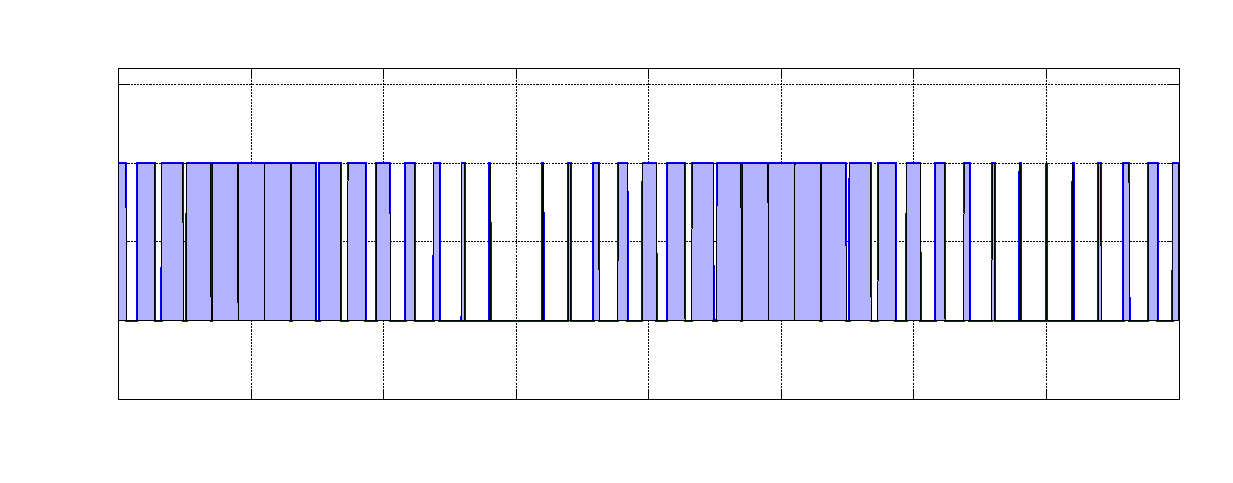
\includegraphics{pwmArea}}%
    \gplfronttext
  \end{picture}%
\endgroup

   %\end{Large}}
   %% Creator: Matplotlib, PGF backend
%%
%% To include the figure in your LaTeX document, write
%%   \input{<filename>.pgf}
%%
%% Make sure the required packages are loaded in your preamble
%%   \usepackage{pgf}
%%
%% Figures using additional raster images can only be included by \input if
%% they are in the same directory as the main LaTeX file. For loading figures
%% from other directories you can use the `import` package
%%   \usepackage{import}
%% and then include the figures with
%%   \import{<path to file>}{<filename>.pgf}
%%
%% Matplotlib used the following preamble
%%   \usepackage[utf8x]{inputenc}
%%   \usepackage[T1]{fontenc}
%%
\begingroup%
\makeatletter%
\begin{pgfpicture}%
\pgfpathrectangle{\pgfpointorigin}{\pgfqpoint{4.317144in}{2.668142in}}%
\pgfusepath{use as bounding box, clip}%
\begin{pgfscope}%
\pgfsetbuttcap%
\pgfsetmiterjoin%
\definecolor{currentfill}{rgb}{1.000000,1.000000,1.000000}%
\pgfsetfillcolor{currentfill}%
\pgfsetlinewidth{0.000000pt}%
\definecolor{currentstroke}{rgb}{1.000000,1.000000,1.000000}%
\pgfsetstrokecolor{currentstroke}%
\pgfsetdash{}{0pt}%
\pgfpathmoveto{\pgfqpoint{0.000000in}{0.000000in}}%
\pgfpathlineto{\pgfqpoint{4.317144in}{0.000000in}}%
\pgfpathlineto{\pgfqpoint{4.317144in}{2.668142in}}%
\pgfpathlineto{\pgfqpoint{0.000000in}{2.668142in}}%
\pgfpathclose%
\pgfusepath{fill}%
\end{pgfscope}%
\begin{pgfscope}%
\pgfsetbuttcap%
\pgfsetmiterjoin%
\definecolor{currentfill}{rgb}{1.000000,1.000000,1.000000}%
\pgfsetfillcolor{currentfill}%
\pgfsetlinewidth{0.000000pt}%
\definecolor{currentstroke}{rgb}{0.000000,0.000000,0.000000}%
\pgfsetstrokecolor{currentstroke}%
\pgfsetstrokeopacity{0.000000}%
\pgfsetdash{}{0pt}%
\pgfpathmoveto{\pgfqpoint{0.594910in}{0.445347in}}%
\pgfpathlineto{\pgfqpoint{4.126298in}{0.445347in}}%
\pgfpathlineto{\pgfqpoint{4.126298in}{2.443163in}}%
\pgfpathlineto{\pgfqpoint{0.594910in}{2.443163in}}%
\pgfpathclose%
\pgfusepath{fill}%
\end{pgfscope}%
\begin{pgfscope}%
\pgfpathrectangle{\pgfqpoint{0.594910in}{0.445347in}}{\pgfqpoint{3.531387in}{1.997816in}} %
\pgfusepath{clip}%
\pgfsetbuttcap%
\pgfsetroundjoin%
\definecolor{currentfill}{rgb}{0.121569,0.466667,0.705882}%
\pgfsetfillcolor{currentfill}%
\pgfsetfillopacity{0.500000}%
\pgfsetlinewidth{0.000000pt}%
\definecolor{currentstroke}{rgb}{0.000000,0.000000,0.000000}%
\pgfsetstrokecolor{currentstroke}%
\pgfsetdash{}{0pt}%
\pgfpathmoveto{\pgfqpoint{0.594910in}{2.110193in}}%
\pgfpathlineto{\pgfqpoint{0.594910in}{0.778316in}}%
\pgfpathlineto{\pgfqpoint{0.595793in}{0.778316in}}%
\pgfpathlineto{\pgfqpoint{0.596677in}{0.778316in}}%
\pgfpathlineto{\pgfqpoint{0.597560in}{0.778316in}}%
\pgfpathlineto{\pgfqpoint{0.598443in}{0.778316in}}%
\pgfpathlineto{\pgfqpoint{0.599326in}{0.778316in}}%
\pgfpathlineto{\pgfqpoint{0.600209in}{0.778316in}}%
\pgfpathlineto{\pgfqpoint{0.601092in}{0.778316in}}%
\pgfpathlineto{\pgfqpoint{0.601975in}{0.778316in}}%
\pgfpathlineto{\pgfqpoint{0.602858in}{0.778316in}}%
\pgfpathlineto{\pgfqpoint{0.603741in}{0.778316in}}%
\pgfpathlineto{\pgfqpoint{0.604624in}{0.778316in}}%
\pgfpathlineto{\pgfqpoint{0.605507in}{0.778316in}}%
\pgfpathlineto{\pgfqpoint{0.606390in}{0.778316in}}%
\pgfpathlineto{\pgfqpoint{0.607273in}{0.778316in}}%
\pgfpathlineto{\pgfqpoint{0.608156in}{0.778316in}}%
\pgfpathlineto{\pgfqpoint{0.609039in}{0.778316in}}%
\pgfpathlineto{\pgfqpoint{0.609923in}{0.778316in}}%
\pgfpathlineto{\pgfqpoint{0.610806in}{0.778316in}}%
\pgfpathlineto{\pgfqpoint{0.611689in}{0.778316in}}%
\pgfpathlineto{\pgfqpoint{0.612572in}{0.778316in}}%
\pgfpathlineto{\pgfqpoint{0.613455in}{0.778316in}}%
\pgfpathlineto{\pgfqpoint{0.614338in}{0.778316in}}%
\pgfpathlineto{\pgfqpoint{0.615221in}{0.778316in}}%
\pgfpathlineto{\pgfqpoint{0.616104in}{0.778316in}}%
\pgfpathlineto{\pgfqpoint{0.616987in}{0.778316in}}%
\pgfpathlineto{\pgfqpoint{0.617870in}{0.778316in}}%
\pgfpathlineto{\pgfqpoint{0.618753in}{0.778316in}}%
\pgfpathlineto{\pgfqpoint{0.619636in}{0.778316in}}%
\pgfpathlineto{\pgfqpoint{0.620519in}{0.778316in}}%
\pgfpathlineto{\pgfqpoint{0.621402in}{0.778316in}}%
\pgfpathlineto{\pgfqpoint{0.622286in}{0.778316in}}%
\pgfpathlineto{\pgfqpoint{0.623169in}{0.778316in}}%
\pgfpathlineto{\pgfqpoint{0.624052in}{0.778316in}}%
\pgfpathlineto{\pgfqpoint{0.624935in}{0.778316in}}%
\pgfpathlineto{\pgfqpoint{0.625818in}{0.778316in}}%
\pgfpathlineto{\pgfqpoint{0.626701in}{0.778316in}}%
\pgfpathlineto{\pgfqpoint{0.627584in}{0.778316in}}%
\pgfpathlineto{\pgfqpoint{0.628467in}{0.778316in}}%
\pgfpathlineto{\pgfqpoint{0.629350in}{0.778316in}}%
\pgfpathlineto{\pgfqpoint{0.630233in}{0.778316in}}%
\pgfpathlineto{\pgfqpoint{0.631116in}{0.778316in}}%
\pgfpathlineto{\pgfqpoint{0.631999in}{0.778316in}}%
\pgfpathlineto{\pgfqpoint{0.632882in}{0.778316in}}%
\pgfpathlineto{\pgfqpoint{0.633765in}{0.778316in}}%
\pgfpathlineto{\pgfqpoint{0.634648in}{0.778316in}}%
\pgfpathlineto{\pgfqpoint{0.635532in}{0.778316in}}%
\pgfpathlineto{\pgfqpoint{0.636415in}{0.778316in}}%
\pgfpathlineto{\pgfqpoint{0.637298in}{0.778316in}}%
\pgfpathlineto{\pgfqpoint{0.638181in}{0.778316in}}%
\pgfpathlineto{\pgfqpoint{0.639064in}{0.778316in}}%
\pgfpathlineto{\pgfqpoint{0.639947in}{0.778316in}}%
\pgfpathlineto{\pgfqpoint{0.640830in}{0.778316in}}%
\pgfpathlineto{\pgfqpoint{0.641713in}{0.778316in}}%
\pgfpathlineto{\pgfqpoint{0.642596in}{0.778316in}}%
\pgfpathlineto{\pgfqpoint{0.643479in}{0.778316in}}%
\pgfpathlineto{\pgfqpoint{0.644362in}{0.778316in}}%
\pgfpathlineto{\pgfqpoint{0.645245in}{0.778316in}}%
\pgfpathlineto{\pgfqpoint{0.646128in}{0.778316in}}%
\pgfpathlineto{\pgfqpoint{0.647011in}{0.778316in}}%
\pgfpathlineto{\pgfqpoint{0.647894in}{0.778316in}}%
\pgfpathlineto{\pgfqpoint{0.648778in}{0.778316in}}%
\pgfpathlineto{\pgfqpoint{0.649661in}{0.778316in}}%
\pgfpathlineto{\pgfqpoint{0.650544in}{0.778316in}}%
\pgfpathlineto{\pgfqpoint{0.651427in}{0.778316in}}%
\pgfpathlineto{\pgfqpoint{0.652310in}{0.778316in}}%
\pgfpathlineto{\pgfqpoint{0.653193in}{0.778316in}}%
\pgfpathlineto{\pgfqpoint{0.654076in}{0.778316in}}%
\pgfpathlineto{\pgfqpoint{0.654959in}{0.778316in}}%
\pgfpathlineto{\pgfqpoint{0.655842in}{0.778316in}}%
\pgfpathlineto{\pgfqpoint{0.656725in}{0.778316in}}%
\pgfpathlineto{\pgfqpoint{0.657608in}{0.778316in}}%
\pgfpathlineto{\pgfqpoint{0.658491in}{0.778316in}}%
\pgfpathlineto{\pgfqpoint{0.659374in}{0.778316in}}%
\pgfpathlineto{\pgfqpoint{0.660257in}{0.778316in}}%
\pgfpathlineto{\pgfqpoint{0.661140in}{0.778316in}}%
\pgfpathlineto{\pgfqpoint{0.662024in}{0.778316in}}%
\pgfpathlineto{\pgfqpoint{0.662907in}{0.778316in}}%
\pgfpathlineto{\pgfqpoint{0.663790in}{0.778316in}}%
\pgfpathlineto{\pgfqpoint{0.664673in}{0.778316in}}%
\pgfpathlineto{\pgfqpoint{0.665556in}{0.778316in}}%
\pgfpathlineto{\pgfqpoint{0.666439in}{0.778316in}}%
\pgfpathlineto{\pgfqpoint{0.667322in}{0.778316in}}%
\pgfpathlineto{\pgfqpoint{0.668205in}{0.778316in}}%
\pgfpathlineto{\pgfqpoint{0.669088in}{0.778316in}}%
\pgfpathlineto{\pgfqpoint{0.669971in}{0.778316in}}%
\pgfpathlineto{\pgfqpoint{0.670854in}{0.778316in}}%
\pgfpathlineto{\pgfqpoint{0.671737in}{0.778316in}}%
\pgfpathlineto{\pgfqpoint{0.672620in}{0.778316in}}%
\pgfpathlineto{\pgfqpoint{0.673503in}{0.778316in}}%
\pgfpathlineto{\pgfqpoint{0.674387in}{0.778316in}}%
\pgfpathlineto{\pgfqpoint{0.675270in}{0.778316in}}%
\pgfpathlineto{\pgfqpoint{0.676153in}{0.778316in}}%
\pgfpathlineto{\pgfqpoint{0.677036in}{0.778316in}}%
\pgfpathlineto{\pgfqpoint{0.677919in}{0.778316in}}%
\pgfpathlineto{\pgfqpoint{0.678802in}{0.778316in}}%
\pgfpathlineto{\pgfqpoint{0.679685in}{0.778316in}}%
\pgfpathlineto{\pgfqpoint{0.680568in}{0.778316in}}%
\pgfpathlineto{\pgfqpoint{0.681451in}{0.778316in}}%
\pgfpathlineto{\pgfqpoint{0.682334in}{0.778316in}}%
\pgfpathlineto{\pgfqpoint{0.683217in}{0.778316in}}%
\pgfpathlineto{\pgfqpoint{0.684100in}{0.778316in}}%
\pgfpathlineto{\pgfqpoint{0.684983in}{0.778316in}}%
\pgfpathlineto{\pgfqpoint{0.685866in}{0.778316in}}%
\pgfpathlineto{\pgfqpoint{0.686749in}{0.778316in}}%
\pgfpathlineto{\pgfqpoint{0.687633in}{0.778316in}}%
\pgfpathlineto{\pgfqpoint{0.688516in}{0.778316in}}%
\pgfpathlineto{\pgfqpoint{0.689399in}{0.778316in}}%
\pgfpathlineto{\pgfqpoint{0.690282in}{0.778316in}}%
\pgfpathlineto{\pgfqpoint{0.691165in}{0.778316in}}%
\pgfpathlineto{\pgfqpoint{0.692048in}{0.778316in}}%
\pgfpathlineto{\pgfqpoint{0.692931in}{0.778316in}}%
\pgfpathlineto{\pgfqpoint{0.693814in}{0.778316in}}%
\pgfpathlineto{\pgfqpoint{0.694697in}{0.778316in}}%
\pgfpathlineto{\pgfqpoint{0.695580in}{0.778316in}}%
\pgfpathlineto{\pgfqpoint{0.696463in}{0.778316in}}%
\pgfpathlineto{\pgfqpoint{0.697346in}{0.778316in}}%
\pgfpathlineto{\pgfqpoint{0.698229in}{0.778316in}}%
\pgfpathlineto{\pgfqpoint{0.699112in}{0.778316in}}%
\pgfpathlineto{\pgfqpoint{0.699995in}{0.778316in}}%
\pgfpathlineto{\pgfqpoint{0.700879in}{0.778316in}}%
\pgfpathlineto{\pgfqpoint{0.701762in}{0.778316in}}%
\pgfpathlineto{\pgfqpoint{0.702645in}{0.778316in}}%
\pgfpathlineto{\pgfqpoint{0.703528in}{0.778316in}}%
\pgfpathlineto{\pgfqpoint{0.704411in}{0.778316in}}%
\pgfpathlineto{\pgfqpoint{0.705294in}{0.778316in}}%
\pgfpathlineto{\pgfqpoint{0.706177in}{0.778316in}}%
\pgfpathlineto{\pgfqpoint{0.707060in}{0.778316in}}%
\pgfpathlineto{\pgfqpoint{0.707943in}{0.778316in}}%
\pgfpathlineto{\pgfqpoint{0.708826in}{0.778316in}}%
\pgfpathlineto{\pgfqpoint{0.709709in}{0.778316in}}%
\pgfpathlineto{\pgfqpoint{0.710592in}{0.778316in}}%
\pgfpathlineto{\pgfqpoint{0.711475in}{0.778316in}}%
\pgfpathlineto{\pgfqpoint{0.712358in}{0.778316in}}%
\pgfpathlineto{\pgfqpoint{0.713241in}{0.778316in}}%
\pgfpathlineto{\pgfqpoint{0.714125in}{0.778316in}}%
\pgfpathlineto{\pgfqpoint{0.715008in}{0.778316in}}%
\pgfpathlineto{\pgfqpoint{0.715891in}{0.778316in}}%
\pgfpathlineto{\pgfqpoint{0.716774in}{0.778316in}}%
\pgfpathlineto{\pgfqpoint{0.717657in}{0.778316in}}%
\pgfpathlineto{\pgfqpoint{0.718540in}{0.778316in}}%
\pgfpathlineto{\pgfqpoint{0.719423in}{0.778316in}}%
\pgfpathlineto{\pgfqpoint{0.720306in}{0.778316in}}%
\pgfpathlineto{\pgfqpoint{0.721189in}{0.778316in}}%
\pgfpathlineto{\pgfqpoint{0.722072in}{0.778316in}}%
\pgfpathlineto{\pgfqpoint{0.722955in}{0.778316in}}%
\pgfpathlineto{\pgfqpoint{0.723838in}{0.778316in}}%
\pgfpathlineto{\pgfqpoint{0.724721in}{0.778316in}}%
\pgfpathlineto{\pgfqpoint{0.725604in}{0.778316in}}%
\pgfpathlineto{\pgfqpoint{0.726487in}{0.778316in}}%
\pgfpathlineto{\pgfqpoint{0.727371in}{0.778316in}}%
\pgfpathlineto{\pgfqpoint{0.728254in}{0.778316in}}%
\pgfpathlineto{\pgfqpoint{0.729137in}{0.778316in}}%
\pgfpathlineto{\pgfqpoint{0.730020in}{0.778316in}}%
\pgfpathlineto{\pgfqpoint{0.730903in}{0.778316in}}%
\pgfpathlineto{\pgfqpoint{0.731786in}{0.778316in}}%
\pgfpathlineto{\pgfqpoint{0.732669in}{0.778316in}}%
\pgfpathlineto{\pgfqpoint{0.733552in}{0.778316in}}%
\pgfpathlineto{\pgfqpoint{0.734435in}{0.778316in}}%
\pgfpathlineto{\pgfqpoint{0.735318in}{0.778316in}}%
\pgfpathlineto{\pgfqpoint{0.736201in}{0.778316in}}%
\pgfpathlineto{\pgfqpoint{0.737084in}{0.778316in}}%
\pgfpathlineto{\pgfqpoint{0.737967in}{0.778316in}}%
\pgfpathlineto{\pgfqpoint{0.738850in}{0.778316in}}%
\pgfpathlineto{\pgfqpoint{0.739734in}{0.778316in}}%
\pgfpathlineto{\pgfqpoint{0.740617in}{0.778316in}}%
\pgfpathlineto{\pgfqpoint{0.741500in}{0.778316in}}%
\pgfpathlineto{\pgfqpoint{0.742383in}{0.778316in}}%
\pgfpathlineto{\pgfqpoint{0.743266in}{0.778316in}}%
\pgfpathlineto{\pgfqpoint{0.744149in}{0.778316in}}%
\pgfpathlineto{\pgfqpoint{0.745032in}{0.778316in}}%
\pgfpathlineto{\pgfqpoint{0.745915in}{0.778316in}}%
\pgfpathlineto{\pgfqpoint{0.746798in}{0.778316in}}%
\pgfpathlineto{\pgfqpoint{0.747681in}{0.778316in}}%
\pgfpathlineto{\pgfqpoint{0.748564in}{0.778316in}}%
\pgfpathlineto{\pgfqpoint{0.749447in}{0.778316in}}%
\pgfpathlineto{\pgfqpoint{0.750330in}{0.778316in}}%
\pgfpathlineto{\pgfqpoint{0.751213in}{0.778316in}}%
\pgfpathlineto{\pgfqpoint{0.752096in}{0.778316in}}%
\pgfpathlineto{\pgfqpoint{0.752980in}{0.778316in}}%
\pgfpathlineto{\pgfqpoint{0.753863in}{0.778316in}}%
\pgfpathlineto{\pgfqpoint{0.754746in}{0.778316in}}%
\pgfpathlineto{\pgfqpoint{0.755629in}{0.778316in}}%
\pgfpathlineto{\pgfqpoint{0.756512in}{0.778316in}}%
\pgfpathlineto{\pgfqpoint{0.757395in}{0.778316in}}%
\pgfpathlineto{\pgfqpoint{0.758278in}{0.778316in}}%
\pgfpathlineto{\pgfqpoint{0.759161in}{0.778316in}}%
\pgfpathlineto{\pgfqpoint{0.760044in}{0.778316in}}%
\pgfpathlineto{\pgfqpoint{0.760927in}{0.778316in}}%
\pgfpathlineto{\pgfqpoint{0.761810in}{0.778316in}}%
\pgfpathlineto{\pgfqpoint{0.762693in}{0.778316in}}%
\pgfpathlineto{\pgfqpoint{0.763576in}{0.778316in}}%
\pgfpathlineto{\pgfqpoint{0.764459in}{0.778316in}}%
\pgfpathlineto{\pgfqpoint{0.765342in}{0.778316in}}%
\pgfpathlineto{\pgfqpoint{0.766226in}{0.778316in}}%
\pgfpathlineto{\pgfqpoint{0.767109in}{0.778316in}}%
\pgfpathlineto{\pgfqpoint{0.767992in}{0.778316in}}%
\pgfpathlineto{\pgfqpoint{0.768875in}{0.778316in}}%
\pgfpathlineto{\pgfqpoint{0.769758in}{0.778316in}}%
\pgfpathlineto{\pgfqpoint{0.770641in}{0.778316in}}%
\pgfpathlineto{\pgfqpoint{0.771524in}{0.778316in}}%
\pgfpathlineto{\pgfqpoint{0.772407in}{0.778316in}}%
\pgfpathlineto{\pgfqpoint{0.773290in}{0.778316in}}%
\pgfpathlineto{\pgfqpoint{0.774173in}{0.778316in}}%
\pgfpathlineto{\pgfqpoint{0.775056in}{0.778316in}}%
\pgfpathlineto{\pgfqpoint{0.775939in}{0.778316in}}%
\pgfpathlineto{\pgfqpoint{0.776822in}{0.778316in}}%
\pgfpathlineto{\pgfqpoint{0.777705in}{0.778316in}}%
\pgfpathlineto{\pgfqpoint{0.778588in}{0.778316in}}%
\pgfpathlineto{\pgfqpoint{0.779472in}{0.778316in}}%
\pgfpathlineto{\pgfqpoint{0.780355in}{0.778316in}}%
\pgfpathlineto{\pgfqpoint{0.781238in}{0.778316in}}%
\pgfpathlineto{\pgfqpoint{0.782121in}{0.778316in}}%
\pgfpathlineto{\pgfqpoint{0.783004in}{0.778316in}}%
\pgfpathlineto{\pgfqpoint{0.783887in}{0.778316in}}%
\pgfpathlineto{\pgfqpoint{0.784770in}{0.778316in}}%
\pgfpathlineto{\pgfqpoint{0.785653in}{0.778316in}}%
\pgfpathlineto{\pgfqpoint{0.786536in}{0.778316in}}%
\pgfpathlineto{\pgfqpoint{0.787419in}{0.778316in}}%
\pgfpathlineto{\pgfqpoint{0.788302in}{0.778316in}}%
\pgfpathlineto{\pgfqpoint{0.789185in}{0.778316in}}%
\pgfpathlineto{\pgfqpoint{0.790068in}{0.778316in}}%
\pgfpathlineto{\pgfqpoint{0.790951in}{0.778316in}}%
\pgfpathlineto{\pgfqpoint{0.791834in}{0.778316in}}%
\pgfpathlineto{\pgfqpoint{0.792718in}{0.778316in}}%
\pgfpathlineto{\pgfqpoint{0.793601in}{0.778316in}}%
\pgfpathlineto{\pgfqpoint{0.794484in}{0.778316in}}%
\pgfpathlineto{\pgfqpoint{0.795367in}{0.778316in}}%
\pgfpathlineto{\pgfqpoint{0.796250in}{0.778316in}}%
\pgfpathlineto{\pgfqpoint{0.797133in}{0.778316in}}%
\pgfpathlineto{\pgfqpoint{0.798016in}{0.778316in}}%
\pgfpathlineto{\pgfqpoint{0.798899in}{0.778316in}}%
\pgfpathlineto{\pgfqpoint{0.799782in}{0.778316in}}%
\pgfpathlineto{\pgfqpoint{0.800665in}{0.778316in}}%
\pgfpathlineto{\pgfqpoint{0.801548in}{0.778316in}}%
\pgfpathlineto{\pgfqpoint{0.802431in}{0.778316in}}%
\pgfpathlineto{\pgfqpoint{0.803314in}{0.778316in}}%
\pgfpathlineto{\pgfqpoint{0.804197in}{0.778316in}}%
\pgfpathlineto{\pgfqpoint{0.805081in}{0.778316in}}%
\pgfpathlineto{\pgfqpoint{0.805964in}{0.778316in}}%
\pgfpathlineto{\pgfqpoint{0.806847in}{0.778316in}}%
\pgfpathlineto{\pgfqpoint{0.807730in}{0.778316in}}%
\pgfpathlineto{\pgfqpoint{0.808613in}{0.778316in}}%
\pgfpathlineto{\pgfqpoint{0.809496in}{0.778316in}}%
\pgfpathlineto{\pgfqpoint{0.810379in}{0.778316in}}%
\pgfpathlineto{\pgfqpoint{0.811262in}{0.778316in}}%
\pgfpathlineto{\pgfqpoint{0.812145in}{0.778316in}}%
\pgfpathlineto{\pgfqpoint{0.813028in}{0.778316in}}%
\pgfpathlineto{\pgfqpoint{0.813911in}{0.778316in}}%
\pgfpathlineto{\pgfqpoint{0.814794in}{0.778316in}}%
\pgfpathlineto{\pgfqpoint{0.815677in}{0.778316in}}%
\pgfpathlineto{\pgfqpoint{0.816560in}{0.778316in}}%
\pgfpathlineto{\pgfqpoint{0.817443in}{0.778316in}}%
\pgfpathlineto{\pgfqpoint{0.818327in}{0.778316in}}%
\pgfpathlineto{\pgfqpoint{0.819210in}{0.778316in}}%
\pgfpathlineto{\pgfqpoint{0.820093in}{0.778316in}}%
\pgfpathlineto{\pgfqpoint{0.820976in}{0.778316in}}%
\pgfpathlineto{\pgfqpoint{0.821859in}{0.778316in}}%
\pgfpathlineto{\pgfqpoint{0.822742in}{0.778316in}}%
\pgfpathlineto{\pgfqpoint{0.823625in}{0.778316in}}%
\pgfpathlineto{\pgfqpoint{0.824508in}{0.778316in}}%
\pgfpathlineto{\pgfqpoint{0.825391in}{0.778316in}}%
\pgfpathlineto{\pgfqpoint{0.826274in}{0.778316in}}%
\pgfpathlineto{\pgfqpoint{0.827157in}{0.778316in}}%
\pgfpathlineto{\pgfqpoint{0.828040in}{0.778316in}}%
\pgfpathlineto{\pgfqpoint{0.828923in}{0.778316in}}%
\pgfpathlineto{\pgfqpoint{0.829806in}{0.778316in}}%
\pgfpathlineto{\pgfqpoint{0.830689in}{0.778316in}}%
\pgfpathlineto{\pgfqpoint{0.831573in}{0.778316in}}%
\pgfpathlineto{\pgfqpoint{0.832456in}{0.778316in}}%
\pgfpathlineto{\pgfqpoint{0.833339in}{0.778316in}}%
\pgfpathlineto{\pgfqpoint{0.834222in}{0.778316in}}%
\pgfpathlineto{\pgfqpoint{0.835105in}{0.778316in}}%
\pgfpathlineto{\pgfqpoint{0.835988in}{0.778316in}}%
\pgfpathlineto{\pgfqpoint{0.836871in}{0.778316in}}%
\pgfpathlineto{\pgfqpoint{0.837754in}{0.778316in}}%
\pgfpathlineto{\pgfqpoint{0.838637in}{0.778316in}}%
\pgfpathlineto{\pgfqpoint{0.839520in}{0.778316in}}%
\pgfpathlineto{\pgfqpoint{0.840403in}{0.778316in}}%
\pgfpathlineto{\pgfqpoint{0.841286in}{0.778316in}}%
\pgfpathlineto{\pgfqpoint{0.842169in}{0.778316in}}%
\pgfpathlineto{\pgfqpoint{0.843052in}{0.778316in}}%
\pgfpathlineto{\pgfqpoint{0.843935in}{0.778316in}}%
\pgfpathlineto{\pgfqpoint{0.844819in}{0.778316in}}%
\pgfpathlineto{\pgfqpoint{0.845702in}{0.778316in}}%
\pgfpathlineto{\pgfqpoint{0.846585in}{0.778316in}}%
\pgfpathlineto{\pgfqpoint{0.847468in}{0.778316in}}%
\pgfpathlineto{\pgfqpoint{0.848351in}{0.778316in}}%
\pgfpathlineto{\pgfqpoint{0.849234in}{0.778316in}}%
\pgfpathlineto{\pgfqpoint{0.850117in}{0.778316in}}%
\pgfpathlineto{\pgfqpoint{0.851000in}{0.778316in}}%
\pgfpathlineto{\pgfqpoint{0.851883in}{0.778316in}}%
\pgfpathlineto{\pgfqpoint{0.852766in}{0.778316in}}%
\pgfpathlineto{\pgfqpoint{0.853649in}{0.778316in}}%
\pgfpathlineto{\pgfqpoint{0.854532in}{0.778316in}}%
\pgfpathlineto{\pgfqpoint{0.855415in}{0.778316in}}%
\pgfpathlineto{\pgfqpoint{0.856298in}{0.778316in}}%
\pgfpathlineto{\pgfqpoint{0.857181in}{0.778316in}}%
\pgfpathlineto{\pgfqpoint{0.858065in}{0.778316in}}%
\pgfpathlineto{\pgfqpoint{0.858948in}{0.778316in}}%
\pgfpathlineto{\pgfqpoint{0.859831in}{0.778316in}}%
\pgfpathlineto{\pgfqpoint{0.860714in}{0.778316in}}%
\pgfpathlineto{\pgfqpoint{0.861597in}{0.778316in}}%
\pgfpathlineto{\pgfqpoint{0.862480in}{0.778316in}}%
\pgfpathlineto{\pgfqpoint{0.863363in}{0.778316in}}%
\pgfpathlineto{\pgfqpoint{0.864246in}{0.778316in}}%
\pgfpathlineto{\pgfqpoint{0.865129in}{0.778316in}}%
\pgfpathlineto{\pgfqpoint{0.866012in}{0.778316in}}%
\pgfpathlineto{\pgfqpoint{0.866895in}{0.778316in}}%
\pgfpathlineto{\pgfqpoint{0.867778in}{0.778316in}}%
\pgfpathlineto{\pgfqpoint{0.868661in}{0.778316in}}%
\pgfpathlineto{\pgfqpoint{0.869544in}{0.778316in}}%
\pgfpathlineto{\pgfqpoint{0.870428in}{0.778316in}}%
\pgfpathlineto{\pgfqpoint{0.871311in}{0.778316in}}%
\pgfpathlineto{\pgfqpoint{0.872194in}{0.778316in}}%
\pgfpathlineto{\pgfqpoint{0.873077in}{0.778316in}}%
\pgfpathlineto{\pgfqpoint{0.873960in}{0.778316in}}%
\pgfpathlineto{\pgfqpoint{0.874843in}{0.778316in}}%
\pgfpathlineto{\pgfqpoint{0.875726in}{0.778316in}}%
\pgfpathlineto{\pgfqpoint{0.876609in}{0.778316in}}%
\pgfpathlineto{\pgfqpoint{0.877492in}{0.778316in}}%
\pgfpathlineto{\pgfqpoint{0.878375in}{0.778316in}}%
\pgfpathlineto{\pgfqpoint{0.879258in}{0.778316in}}%
\pgfpathlineto{\pgfqpoint{0.880141in}{0.778316in}}%
\pgfpathlineto{\pgfqpoint{0.881024in}{0.778316in}}%
\pgfpathlineto{\pgfqpoint{0.881907in}{0.778316in}}%
\pgfpathlineto{\pgfqpoint{0.882790in}{0.778316in}}%
\pgfpathlineto{\pgfqpoint{0.883674in}{0.778316in}}%
\pgfpathlineto{\pgfqpoint{0.884557in}{0.778316in}}%
\pgfpathlineto{\pgfqpoint{0.885440in}{0.778316in}}%
\pgfpathlineto{\pgfqpoint{0.886323in}{0.778316in}}%
\pgfpathlineto{\pgfqpoint{0.887206in}{0.778316in}}%
\pgfpathlineto{\pgfqpoint{0.888089in}{0.778316in}}%
\pgfpathlineto{\pgfqpoint{0.888972in}{0.778316in}}%
\pgfpathlineto{\pgfqpoint{0.889855in}{0.778316in}}%
\pgfpathlineto{\pgfqpoint{0.890738in}{0.778316in}}%
\pgfpathlineto{\pgfqpoint{0.891621in}{0.778316in}}%
\pgfpathlineto{\pgfqpoint{0.892504in}{0.778316in}}%
\pgfpathlineto{\pgfqpoint{0.893387in}{0.778316in}}%
\pgfpathlineto{\pgfqpoint{0.894270in}{0.778316in}}%
\pgfpathlineto{\pgfqpoint{0.895153in}{0.778316in}}%
\pgfpathlineto{\pgfqpoint{0.896036in}{0.778316in}}%
\pgfpathlineto{\pgfqpoint{0.896920in}{0.778316in}}%
\pgfpathlineto{\pgfqpoint{0.897803in}{0.778316in}}%
\pgfpathlineto{\pgfqpoint{0.898686in}{0.778316in}}%
\pgfpathlineto{\pgfqpoint{0.899569in}{0.778316in}}%
\pgfpathlineto{\pgfqpoint{0.900452in}{0.778316in}}%
\pgfpathlineto{\pgfqpoint{0.901335in}{0.778316in}}%
\pgfpathlineto{\pgfqpoint{0.902218in}{0.778316in}}%
\pgfpathlineto{\pgfqpoint{0.903101in}{0.778316in}}%
\pgfpathlineto{\pgfqpoint{0.903984in}{0.778316in}}%
\pgfpathlineto{\pgfqpoint{0.904867in}{0.778316in}}%
\pgfpathlineto{\pgfqpoint{0.905750in}{0.778316in}}%
\pgfpathlineto{\pgfqpoint{0.906633in}{0.778316in}}%
\pgfpathlineto{\pgfqpoint{0.907516in}{0.778316in}}%
\pgfpathlineto{\pgfqpoint{0.908399in}{0.778316in}}%
\pgfpathlineto{\pgfqpoint{0.909282in}{0.778316in}}%
\pgfpathlineto{\pgfqpoint{0.910166in}{0.778316in}}%
\pgfpathlineto{\pgfqpoint{0.911049in}{0.778316in}}%
\pgfpathlineto{\pgfqpoint{0.911932in}{0.778316in}}%
\pgfpathlineto{\pgfqpoint{0.912815in}{0.778316in}}%
\pgfpathlineto{\pgfqpoint{0.913698in}{0.778316in}}%
\pgfpathlineto{\pgfqpoint{0.914581in}{0.778316in}}%
\pgfpathlineto{\pgfqpoint{0.915464in}{0.778316in}}%
\pgfpathlineto{\pgfqpoint{0.916347in}{0.778316in}}%
\pgfpathlineto{\pgfqpoint{0.917230in}{0.778316in}}%
\pgfpathlineto{\pgfqpoint{0.918113in}{0.778316in}}%
\pgfpathlineto{\pgfqpoint{0.918996in}{0.778316in}}%
\pgfpathlineto{\pgfqpoint{0.919879in}{0.778316in}}%
\pgfpathlineto{\pgfqpoint{0.920762in}{0.778316in}}%
\pgfpathlineto{\pgfqpoint{0.921645in}{0.778316in}}%
\pgfpathlineto{\pgfqpoint{0.922528in}{0.778316in}}%
\pgfpathlineto{\pgfqpoint{0.923412in}{0.778316in}}%
\pgfpathlineto{\pgfqpoint{0.924295in}{0.778316in}}%
\pgfpathlineto{\pgfqpoint{0.925178in}{0.778316in}}%
\pgfpathlineto{\pgfqpoint{0.926061in}{0.778316in}}%
\pgfpathlineto{\pgfqpoint{0.926944in}{0.778316in}}%
\pgfpathlineto{\pgfqpoint{0.927827in}{0.778316in}}%
\pgfpathlineto{\pgfqpoint{0.928710in}{0.778316in}}%
\pgfpathlineto{\pgfqpoint{0.929593in}{0.778316in}}%
\pgfpathlineto{\pgfqpoint{0.930476in}{0.778316in}}%
\pgfpathlineto{\pgfqpoint{0.931359in}{0.778316in}}%
\pgfpathlineto{\pgfqpoint{0.932242in}{0.778316in}}%
\pgfpathlineto{\pgfqpoint{0.933125in}{0.778316in}}%
\pgfpathlineto{\pgfqpoint{0.934008in}{0.778316in}}%
\pgfpathlineto{\pgfqpoint{0.934891in}{0.778316in}}%
\pgfpathlineto{\pgfqpoint{0.935775in}{0.778316in}}%
\pgfpathlineto{\pgfqpoint{0.936658in}{0.778316in}}%
\pgfpathlineto{\pgfqpoint{0.937541in}{0.778316in}}%
\pgfpathlineto{\pgfqpoint{0.938424in}{0.778316in}}%
\pgfpathlineto{\pgfqpoint{0.939307in}{0.778316in}}%
\pgfpathlineto{\pgfqpoint{0.940190in}{0.778316in}}%
\pgfpathlineto{\pgfqpoint{0.941073in}{0.778316in}}%
\pgfpathlineto{\pgfqpoint{0.941956in}{0.778316in}}%
\pgfpathlineto{\pgfqpoint{0.942839in}{0.778316in}}%
\pgfpathlineto{\pgfqpoint{0.943722in}{0.778316in}}%
\pgfpathlineto{\pgfqpoint{0.944605in}{0.778316in}}%
\pgfpathlineto{\pgfqpoint{0.945488in}{0.778316in}}%
\pgfpathlineto{\pgfqpoint{0.946371in}{0.778316in}}%
\pgfpathlineto{\pgfqpoint{0.947254in}{0.778316in}}%
\pgfpathlineto{\pgfqpoint{0.948137in}{0.778316in}}%
\pgfpathlineto{\pgfqpoint{0.949021in}{0.778316in}}%
\pgfpathlineto{\pgfqpoint{0.949904in}{0.778316in}}%
\pgfpathlineto{\pgfqpoint{0.950787in}{0.778316in}}%
\pgfpathlineto{\pgfqpoint{0.951670in}{0.778316in}}%
\pgfpathlineto{\pgfqpoint{0.952553in}{0.778316in}}%
\pgfpathlineto{\pgfqpoint{0.953436in}{0.778316in}}%
\pgfpathlineto{\pgfqpoint{0.954319in}{0.778316in}}%
\pgfpathlineto{\pgfqpoint{0.955202in}{0.778316in}}%
\pgfpathlineto{\pgfqpoint{0.956085in}{0.778316in}}%
\pgfpathlineto{\pgfqpoint{0.956968in}{0.778316in}}%
\pgfpathlineto{\pgfqpoint{0.957851in}{0.778316in}}%
\pgfpathlineto{\pgfqpoint{0.958734in}{0.778316in}}%
\pgfpathlineto{\pgfqpoint{0.959617in}{0.778316in}}%
\pgfpathlineto{\pgfqpoint{0.960500in}{0.778316in}}%
\pgfpathlineto{\pgfqpoint{0.961383in}{0.778316in}}%
\pgfpathlineto{\pgfqpoint{0.962267in}{0.778316in}}%
\pgfpathlineto{\pgfqpoint{0.963150in}{0.778316in}}%
\pgfpathlineto{\pgfqpoint{0.964033in}{0.778316in}}%
\pgfpathlineto{\pgfqpoint{0.964916in}{0.778316in}}%
\pgfpathlineto{\pgfqpoint{0.965799in}{0.778316in}}%
\pgfpathlineto{\pgfqpoint{0.966682in}{0.778316in}}%
\pgfpathlineto{\pgfqpoint{0.967565in}{0.778316in}}%
\pgfpathlineto{\pgfqpoint{0.968448in}{0.778316in}}%
\pgfpathlineto{\pgfqpoint{0.969331in}{0.778316in}}%
\pgfpathlineto{\pgfqpoint{0.970214in}{0.778316in}}%
\pgfpathlineto{\pgfqpoint{0.971097in}{0.778316in}}%
\pgfpathlineto{\pgfqpoint{0.971980in}{0.778316in}}%
\pgfpathlineto{\pgfqpoint{0.972863in}{0.778316in}}%
\pgfpathlineto{\pgfqpoint{0.973746in}{0.778316in}}%
\pgfpathlineto{\pgfqpoint{0.974629in}{0.778316in}}%
\pgfpathlineto{\pgfqpoint{0.975513in}{0.778316in}}%
\pgfpathlineto{\pgfqpoint{0.976396in}{0.778316in}}%
\pgfpathlineto{\pgfqpoint{0.977279in}{0.778316in}}%
\pgfpathlineto{\pgfqpoint{0.978162in}{0.778316in}}%
\pgfpathlineto{\pgfqpoint{0.979045in}{0.778316in}}%
\pgfpathlineto{\pgfqpoint{0.979928in}{0.778316in}}%
\pgfpathlineto{\pgfqpoint{0.980811in}{0.778316in}}%
\pgfpathlineto{\pgfqpoint{0.981694in}{0.778316in}}%
\pgfpathlineto{\pgfqpoint{0.982577in}{0.778316in}}%
\pgfpathlineto{\pgfqpoint{0.983460in}{0.778316in}}%
\pgfpathlineto{\pgfqpoint{0.984343in}{0.778316in}}%
\pgfpathlineto{\pgfqpoint{0.985226in}{0.778316in}}%
\pgfpathlineto{\pgfqpoint{0.986109in}{0.778316in}}%
\pgfpathlineto{\pgfqpoint{0.986992in}{0.778316in}}%
\pgfpathlineto{\pgfqpoint{0.987875in}{0.778316in}}%
\pgfpathlineto{\pgfqpoint{0.988759in}{0.778316in}}%
\pgfpathlineto{\pgfqpoint{0.989642in}{0.778316in}}%
\pgfpathlineto{\pgfqpoint{0.990525in}{0.778316in}}%
\pgfpathlineto{\pgfqpoint{0.991408in}{0.778316in}}%
\pgfpathlineto{\pgfqpoint{0.992291in}{0.778316in}}%
\pgfpathlineto{\pgfqpoint{0.993174in}{0.778316in}}%
\pgfpathlineto{\pgfqpoint{0.994057in}{0.778316in}}%
\pgfpathlineto{\pgfqpoint{0.994940in}{0.778316in}}%
\pgfpathlineto{\pgfqpoint{0.995823in}{0.778316in}}%
\pgfpathlineto{\pgfqpoint{0.996706in}{0.778316in}}%
\pgfpathlineto{\pgfqpoint{0.997589in}{0.778316in}}%
\pgfpathlineto{\pgfqpoint{0.998472in}{0.778316in}}%
\pgfpathlineto{\pgfqpoint{0.999355in}{0.778316in}}%
\pgfpathlineto{\pgfqpoint{1.000238in}{0.778316in}}%
\pgfpathlineto{\pgfqpoint{1.001122in}{0.778316in}}%
\pgfpathlineto{\pgfqpoint{1.002005in}{0.778316in}}%
\pgfpathlineto{\pgfqpoint{1.002888in}{0.778316in}}%
\pgfpathlineto{\pgfqpoint{1.003771in}{0.778316in}}%
\pgfpathlineto{\pgfqpoint{1.004654in}{0.778316in}}%
\pgfpathlineto{\pgfqpoint{1.005537in}{0.778316in}}%
\pgfpathlineto{\pgfqpoint{1.006420in}{0.778316in}}%
\pgfpathlineto{\pgfqpoint{1.007303in}{0.778316in}}%
\pgfpathlineto{\pgfqpoint{1.008186in}{0.778316in}}%
\pgfpathlineto{\pgfqpoint{1.009069in}{0.778316in}}%
\pgfpathlineto{\pgfqpoint{1.009952in}{0.778316in}}%
\pgfpathlineto{\pgfqpoint{1.010835in}{0.778316in}}%
\pgfpathlineto{\pgfqpoint{1.011718in}{0.778316in}}%
\pgfpathlineto{\pgfqpoint{1.012601in}{0.778316in}}%
\pgfpathlineto{\pgfqpoint{1.013484in}{0.778316in}}%
\pgfpathlineto{\pgfqpoint{1.014368in}{0.778316in}}%
\pgfpathlineto{\pgfqpoint{1.015251in}{0.778316in}}%
\pgfpathlineto{\pgfqpoint{1.016134in}{0.778316in}}%
\pgfpathlineto{\pgfqpoint{1.017017in}{0.778316in}}%
\pgfpathlineto{\pgfqpoint{1.017900in}{0.778316in}}%
\pgfpathlineto{\pgfqpoint{1.018783in}{0.778316in}}%
\pgfpathlineto{\pgfqpoint{1.019666in}{0.778316in}}%
\pgfpathlineto{\pgfqpoint{1.020549in}{0.778316in}}%
\pgfpathlineto{\pgfqpoint{1.021432in}{0.778316in}}%
\pgfpathlineto{\pgfqpoint{1.022315in}{0.778316in}}%
\pgfpathlineto{\pgfqpoint{1.023198in}{0.778316in}}%
\pgfpathlineto{\pgfqpoint{1.024081in}{0.778316in}}%
\pgfpathlineto{\pgfqpoint{1.024964in}{0.778316in}}%
\pgfpathlineto{\pgfqpoint{1.025847in}{0.778316in}}%
\pgfpathlineto{\pgfqpoint{1.026730in}{0.778316in}}%
\pgfpathlineto{\pgfqpoint{1.027614in}{0.778316in}}%
\pgfpathlineto{\pgfqpoint{1.028497in}{0.778316in}}%
\pgfpathlineto{\pgfqpoint{1.029380in}{0.778316in}}%
\pgfpathlineto{\pgfqpoint{1.030263in}{0.778316in}}%
\pgfpathlineto{\pgfqpoint{1.031146in}{0.778316in}}%
\pgfpathlineto{\pgfqpoint{1.032029in}{0.778316in}}%
\pgfpathlineto{\pgfqpoint{1.032912in}{0.778316in}}%
\pgfpathlineto{\pgfqpoint{1.033795in}{0.778316in}}%
\pgfpathlineto{\pgfqpoint{1.034678in}{0.778316in}}%
\pgfpathlineto{\pgfqpoint{1.035561in}{0.778316in}}%
\pgfpathlineto{\pgfqpoint{1.036444in}{0.778316in}}%
\pgfpathlineto{\pgfqpoint{1.037327in}{0.778316in}}%
\pgfpathlineto{\pgfqpoint{1.038210in}{0.778316in}}%
\pgfpathlineto{\pgfqpoint{1.039093in}{0.778316in}}%
\pgfpathlineto{\pgfqpoint{1.039976in}{0.778316in}}%
\pgfpathlineto{\pgfqpoint{1.040860in}{0.778316in}}%
\pgfpathlineto{\pgfqpoint{1.041743in}{0.778316in}}%
\pgfpathlineto{\pgfqpoint{1.042626in}{0.778316in}}%
\pgfpathlineto{\pgfqpoint{1.043509in}{0.778316in}}%
\pgfpathlineto{\pgfqpoint{1.044392in}{0.778316in}}%
\pgfpathlineto{\pgfqpoint{1.045275in}{0.778316in}}%
\pgfpathlineto{\pgfqpoint{1.046158in}{0.778316in}}%
\pgfpathlineto{\pgfqpoint{1.047041in}{0.778316in}}%
\pgfpathlineto{\pgfqpoint{1.047924in}{0.778316in}}%
\pgfpathlineto{\pgfqpoint{1.048807in}{0.778316in}}%
\pgfpathlineto{\pgfqpoint{1.049690in}{0.778316in}}%
\pgfpathlineto{\pgfqpoint{1.050573in}{0.778316in}}%
\pgfpathlineto{\pgfqpoint{1.051456in}{0.778316in}}%
\pgfpathlineto{\pgfqpoint{1.052339in}{0.778316in}}%
\pgfpathlineto{\pgfqpoint{1.053222in}{0.778316in}}%
\pgfpathlineto{\pgfqpoint{1.054106in}{0.778316in}}%
\pgfpathlineto{\pgfqpoint{1.054989in}{0.778316in}}%
\pgfpathlineto{\pgfqpoint{1.055872in}{0.778316in}}%
\pgfpathlineto{\pgfqpoint{1.056755in}{0.778316in}}%
\pgfpathlineto{\pgfqpoint{1.057638in}{0.778316in}}%
\pgfpathlineto{\pgfqpoint{1.058521in}{0.778316in}}%
\pgfpathlineto{\pgfqpoint{1.059404in}{0.778316in}}%
\pgfpathlineto{\pgfqpoint{1.060287in}{0.778316in}}%
\pgfpathlineto{\pgfqpoint{1.061170in}{0.778316in}}%
\pgfpathlineto{\pgfqpoint{1.062053in}{0.778316in}}%
\pgfpathlineto{\pgfqpoint{1.062936in}{0.778316in}}%
\pgfpathlineto{\pgfqpoint{1.063819in}{0.778316in}}%
\pgfpathlineto{\pgfqpoint{1.064702in}{0.778316in}}%
\pgfpathlineto{\pgfqpoint{1.065585in}{0.778316in}}%
\pgfpathlineto{\pgfqpoint{1.066469in}{0.778316in}}%
\pgfpathlineto{\pgfqpoint{1.067352in}{0.778316in}}%
\pgfpathlineto{\pgfqpoint{1.068235in}{0.778316in}}%
\pgfpathlineto{\pgfqpoint{1.069118in}{0.778316in}}%
\pgfpathlineto{\pgfqpoint{1.070001in}{0.778316in}}%
\pgfpathlineto{\pgfqpoint{1.070884in}{0.778316in}}%
\pgfpathlineto{\pgfqpoint{1.071767in}{0.778316in}}%
\pgfpathlineto{\pgfqpoint{1.072650in}{0.778316in}}%
\pgfpathlineto{\pgfqpoint{1.073533in}{0.778316in}}%
\pgfpathlineto{\pgfqpoint{1.074416in}{0.778316in}}%
\pgfpathlineto{\pgfqpoint{1.075299in}{0.778316in}}%
\pgfpathlineto{\pgfqpoint{1.076182in}{0.778316in}}%
\pgfpathlineto{\pgfqpoint{1.077065in}{0.778316in}}%
\pgfpathlineto{\pgfqpoint{1.077948in}{0.778316in}}%
\pgfpathlineto{\pgfqpoint{1.078831in}{0.778316in}}%
\pgfpathlineto{\pgfqpoint{1.079715in}{0.778316in}}%
\pgfpathlineto{\pgfqpoint{1.080598in}{0.778316in}}%
\pgfpathlineto{\pgfqpoint{1.081481in}{0.778316in}}%
\pgfpathlineto{\pgfqpoint{1.082364in}{0.778316in}}%
\pgfpathlineto{\pgfqpoint{1.083247in}{0.778316in}}%
\pgfpathlineto{\pgfqpoint{1.084130in}{0.778316in}}%
\pgfpathlineto{\pgfqpoint{1.085013in}{0.778316in}}%
\pgfpathlineto{\pgfqpoint{1.085896in}{0.778316in}}%
\pgfpathlineto{\pgfqpoint{1.086779in}{0.778316in}}%
\pgfpathlineto{\pgfqpoint{1.087662in}{0.778316in}}%
\pgfpathlineto{\pgfqpoint{1.088545in}{0.778316in}}%
\pgfpathlineto{\pgfqpoint{1.089428in}{0.778316in}}%
\pgfpathlineto{\pgfqpoint{1.090311in}{0.778316in}}%
\pgfpathlineto{\pgfqpoint{1.091194in}{0.778316in}}%
\pgfpathlineto{\pgfqpoint{1.092077in}{0.778316in}}%
\pgfpathlineto{\pgfqpoint{1.092961in}{0.778316in}}%
\pgfpathlineto{\pgfqpoint{1.093844in}{0.778316in}}%
\pgfpathlineto{\pgfqpoint{1.094727in}{0.778316in}}%
\pgfpathlineto{\pgfqpoint{1.095610in}{0.778316in}}%
\pgfpathlineto{\pgfqpoint{1.096493in}{0.778316in}}%
\pgfpathlineto{\pgfqpoint{1.097376in}{0.778316in}}%
\pgfpathlineto{\pgfqpoint{1.098259in}{0.778316in}}%
\pgfpathlineto{\pgfqpoint{1.099142in}{0.778316in}}%
\pgfpathlineto{\pgfqpoint{1.100025in}{0.778316in}}%
\pgfpathlineto{\pgfqpoint{1.100908in}{0.778316in}}%
\pgfpathlineto{\pgfqpoint{1.101791in}{0.778316in}}%
\pgfpathlineto{\pgfqpoint{1.102674in}{0.778316in}}%
\pgfpathlineto{\pgfqpoint{1.103557in}{0.778316in}}%
\pgfpathlineto{\pgfqpoint{1.104440in}{0.778316in}}%
\pgfpathlineto{\pgfqpoint{1.105323in}{0.778316in}}%
\pgfpathlineto{\pgfqpoint{1.106207in}{0.778316in}}%
\pgfpathlineto{\pgfqpoint{1.107090in}{0.778316in}}%
\pgfpathlineto{\pgfqpoint{1.107973in}{0.778316in}}%
\pgfpathlineto{\pgfqpoint{1.108856in}{0.778316in}}%
\pgfpathlineto{\pgfqpoint{1.109739in}{0.778316in}}%
\pgfpathlineto{\pgfqpoint{1.110622in}{0.778316in}}%
\pgfpathlineto{\pgfqpoint{1.111505in}{0.778316in}}%
\pgfpathlineto{\pgfqpoint{1.112388in}{0.778316in}}%
\pgfpathlineto{\pgfqpoint{1.113271in}{0.778316in}}%
\pgfpathlineto{\pgfqpoint{1.114154in}{0.778316in}}%
\pgfpathlineto{\pgfqpoint{1.115037in}{0.778316in}}%
\pgfpathlineto{\pgfqpoint{1.115920in}{0.778316in}}%
\pgfpathlineto{\pgfqpoint{1.116803in}{0.778316in}}%
\pgfpathlineto{\pgfqpoint{1.117686in}{0.778316in}}%
\pgfpathlineto{\pgfqpoint{1.118570in}{0.778316in}}%
\pgfpathlineto{\pgfqpoint{1.119453in}{0.778316in}}%
\pgfpathlineto{\pgfqpoint{1.120336in}{0.778316in}}%
\pgfpathlineto{\pgfqpoint{1.121219in}{0.778316in}}%
\pgfpathlineto{\pgfqpoint{1.122102in}{0.778316in}}%
\pgfpathlineto{\pgfqpoint{1.122985in}{0.778316in}}%
\pgfpathlineto{\pgfqpoint{1.123868in}{0.778316in}}%
\pgfpathlineto{\pgfqpoint{1.124751in}{0.778316in}}%
\pgfpathlineto{\pgfqpoint{1.125634in}{0.778316in}}%
\pgfpathlineto{\pgfqpoint{1.126517in}{0.778316in}}%
\pgfpathlineto{\pgfqpoint{1.127400in}{0.778316in}}%
\pgfpathlineto{\pgfqpoint{1.128283in}{0.778316in}}%
\pgfpathlineto{\pgfqpoint{1.129166in}{0.778316in}}%
\pgfpathlineto{\pgfqpoint{1.130049in}{0.778316in}}%
\pgfpathlineto{\pgfqpoint{1.130932in}{0.778316in}}%
\pgfpathlineto{\pgfqpoint{1.131816in}{0.778316in}}%
\pgfpathlineto{\pgfqpoint{1.132699in}{0.778316in}}%
\pgfpathlineto{\pgfqpoint{1.133582in}{0.778316in}}%
\pgfpathlineto{\pgfqpoint{1.134465in}{0.778316in}}%
\pgfpathlineto{\pgfqpoint{1.135348in}{0.778316in}}%
\pgfpathlineto{\pgfqpoint{1.136231in}{0.778316in}}%
\pgfpathlineto{\pgfqpoint{1.137114in}{0.778316in}}%
\pgfpathlineto{\pgfqpoint{1.137997in}{0.778316in}}%
\pgfpathlineto{\pgfqpoint{1.138880in}{0.778316in}}%
\pgfpathlineto{\pgfqpoint{1.139763in}{0.778316in}}%
\pgfpathlineto{\pgfqpoint{1.140646in}{0.778316in}}%
\pgfpathlineto{\pgfqpoint{1.141529in}{0.778316in}}%
\pgfpathlineto{\pgfqpoint{1.142412in}{0.778316in}}%
\pgfpathlineto{\pgfqpoint{1.143295in}{0.778316in}}%
\pgfpathlineto{\pgfqpoint{1.144178in}{0.778316in}}%
\pgfpathlineto{\pgfqpoint{1.145062in}{0.778316in}}%
\pgfpathlineto{\pgfqpoint{1.145945in}{0.778316in}}%
\pgfpathlineto{\pgfqpoint{1.146828in}{0.778316in}}%
\pgfpathlineto{\pgfqpoint{1.147711in}{0.778316in}}%
\pgfpathlineto{\pgfqpoint{1.148594in}{0.778316in}}%
\pgfpathlineto{\pgfqpoint{1.149477in}{0.778316in}}%
\pgfpathlineto{\pgfqpoint{1.150360in}{0.778316in}}%
\pgfpathlineto{\pgfqpoint{1.151243in}{0.778316in}}%
\pgfpathlineto{\pgfqpoint{1.152126in}{0.778316in}}%
\pgfpathlineto{\pgfqpoint{1.153009in}{0.778316in}}%
\pgfpathlineto{\pgfqpoint{1.153892in}{0.778316in}}%
\pgfpathlineto{\pgfqpoint{1.154775in}{0.778316in}}%
\pgfpathlineto{\pgfqpoint{1.155658in}{0.778316in}}%
\pgfpathlineto{\pgfqpoint{1.156541in}{0.778316in}}%
\pgfpathlineto{\pgfqpoint{1.157424in}{0.778316in}}%
\pgfpathlineto{\pgfqpoint{1.158308in}{0.778316in}}%
\pgfpathlineto{\pgfqpoint{1.159191in}{0.778316in}}%
\pgfpathlineto{\pgfqpoint{1.160074in}{0.778316in}}%
\pgfpathlineto{\pgfqpoint{1.160957in}{0.778316in}}%
\pgfpathlineto{\pgfqpoint{1.161840in}{0.778316in}}%
\pgfpathlineto{\pgfqpoint{1.162723in}{0.778316in}}%
\pgfpathlineto{\pgfqpoint{1.163606in}{0.778316in}}%
\pgfpathlineto{\pgfqpoint{1.164489in}{0.778316in}}%
\pgfpathlineto{\pgfqpoint{1.165372in}{0.778316in}}%
\pgfpathlineto{\pgfqpoint{1.166255in}{0.778316in}}%
\pgfpathlineto{\pgfqpoint{1.167138in}{0.778316in}}%
\pgfpathlineto{\pgfqpoint{1.168021in}{0.778316in}}%
\pgfpathlineto{\pgfqpoint{1.168904in}{0.778316in}}%
\pgfpathlineto{\pgfqpoint{1.169787in}{0.778316in}}%
\pgfpathlineto{\pgfqpoint{1.170670in}{0.778316in}}%
\pgfpathlineto{\pgfqpoint{1.171554in}{0.778316in}}%
\pgfpathlineto{\pgfqpoint{1.172437in}{0.778316in}}%
\pgfpathlineto{\pgfqpoint{1.173320in}{0.778316in}}%
\pgfpathlineto{\pgfqpoint{1.174203in}{0.778316in}}%
\pgfpathlineto{\pgfqpoint{1.175086in}{0.778316in}}%
\pgfpathlineto{\pgfqpoint{1.175969in}{0.778316in}}%
\pgfpathlineto{\pgfqpoint{1.176852in}{0.778316in}}%
\pgfpathlineto{\pgfqpoint{1.177735in}{0.778316in}}%
\pgfpathlineto{\pgfqpoint{1.178618in}{0.778316in}}%
\pgfpathlineto{\pgfqpoint{1.179501in}{0.778316in}}%
\pgfpathlineto{\pgfqpoint{1.180384in}{0.778316in}}%
\pgfpathlineto{\pgfqpoint{1.181267in}{0.778316in}}%
\pgfpathlineto{\pgfqpoint{1.182150in}{0.778316in}}%
\pgfpathlineto{\pgfqpoint{1.183033in}{0.778316in}}%
\pgfpathlineto{\pgfqpoint{1.183917in}{0.778316in}}%
\pgfpathlineto{\pgfqpoint{1.184800in}{0.778316in}}%
\pgfpathlineto{\pgfqpoint{1.185683in}{0.778316in}}%
\pgfpathlineto{\pgfqpoint{1.186566in}{0.778316in}}%
\pgfpathlineto{\pgfqpoint{1.187449in}{0.778316in}}%
\pgfpathlineto{\pgfqpoint{1.188332in}{0.778316in}}%
\pgfpathlineto{\pgfqpoint{1.189215in}{0.778316in}}%
\pgfpathlineto{\pgfqpoint{1.190098in}{0.778316in}}%
\pgfpathlineto{\pgfqpoint{1.190981in}{0.778316in}}%
\pgfpathlineto{\pgfqpoint{1.191864in}{0.778316in}}%
\pgfpathlineto{\pgfqpoint{1.192747in}{0.778316in}}%
\pgfpathlineto{\pgfqpoint{1.193630in}{0.778316in}}%
\pgfpathlineto{\pgfqpoint{1.194513in}{0.778316in}}%
\pgfpathlineto{\pgfqpoint{1.195396in}{0.778316in}}%
\pgfpathlineto{\pgfqpoint{1.196279in}{0.778316in}}%
\pgfpathlineto{\pgfqpoint{1.197163in}{0.778316in}}%
\pgfpathlineto{\pgfqpoint{1.198046in}{0.778316in}}%
\pgfpathlineto{\pgfqpoint{1.198929in}{0.778316in}}%
\pgfpathlineto{\pgfqpoint{1.199812in}{0.778316in}}%
\pgfpathlineto{\pgfqpoint{1.200695in}{0.778316in}}%
\pgfpathlineto{\pgfqpoint{1.201578in}{0.778316in}}%
\pgfpathlineto{\pgfqpoint{1.202461in}{0.778316in}}%
\pgfpathlineto{\pgfqpoint{1.203344in}{0.778316in}}%
\pgfpathlineto{\pgfqpoint{1.204227in}{0.778316in}}%
\pgfpathlineto{\pgfqpoint{1.205110in}{0.778316in}}%
\pgfpathlineto{\pgfqpoint{1.205993in}{0.778316in}}%
\pgfpathlineto{\pgfqpoint{1.206876in}{0.778316in}}%
\pgfpathlineto{\pgfqpoint{1.207759in}{0.778316in}}%
\pgfpathlineto{\pgfqpoint{1.208642in}{0.778316in}}%
\pgfpathlineto{\pgfqpoint{1.209525in}{0.778316in}}%
\pgfpathlineto{\pgfqpoint{1.210409in}{0.778316in}}%
\pgfpathlineto{\pgfqpoint{1.211292in}{0.778316in}}%
\pgfpathlineto{\pgfqpoint{1.212175in}{0.778316in}}%
\pgfpathlineto{\pgfqpoint{1.213058in}{0.778316in}}%
\pgfpathlineto{\pgfqpoint{1.213941in}{0.778316in}}%
\pgfpathlineto{\pgfqpoint{1.214824in}{0.778316in}}%
\pgfpathlineto{\pgfqpoint{1.215707in}{0.778316in}}%
\pgfpathlineto{\pgfqpoint{1.216590in}{0.778316in}}%
\pgfpathlineto{\pgfqpoint{1.217473in}{0.778316in}}%
\pgfpathlineto{\pgfqpoint{1.218356in}{0.778316in}}%
\pgfpathlineto{\pgfqpoint{1.219239in}{0.778316in}}%
\pgfpathlineto{\pgfqpoint{1.220122in}{0.778316in}}%
\pgfpathlineto{\pgfqpoint{1.221005in}{0.778316in}}%
\pgfpathlineto{\pgfqpoint{1.221888in}{0.778316in}}%
\pgfpathlineto{\pgfqpoint{1.222771in}{0.778316in}}%
\pgfpathlineto{\pgfqpoint{1.223655in}{0.778316in}}%
\pgfpathlineto{\pgfqpoint{1.224538in}{0.778316in}}%
\pgfpathlineto{\pgfqpoint{1.225421in}{0.778316in}}%
\pgfpathlineto{\pgfqpoint{1.226304in}{0.778316in}}%
\pgfpathlineto{\pgfqpoint{1.227187in}{0.778316in}}%
\pgfpathlineto{\pgfqpoint{1.228070in}{0.778316in}}%
\pgfpathlineto{\pgfqpoint{1.228953in}{0.778316in}}%
\pgfpathlineto{\pgfqpoint{1.229836in}{0.778316in}}%
\pgfpathlineto{\pgfqpoint{1.230719in}{0.778316in}}%
\pgfpathlineto{\pgfqpoint{1.231602in}{0.778316in}}%
\pgfpathlineto{\pgfqpoint{1.232485in}{0.778316in}}%
\pgfpathlineto{\pgfqpoint{1.233368in}{0.778316in}}%
\pgfpathlineto{\pgfqpoint{1.234251in}{0.778316in}}%
\pgfpathlineto{\pgfqpoint{1.235134in}{0.778316in}}%
\pgfpathlineto{\pgfqpoint{1.236017in}{0.778316in}}%
\pgfpathlineto{\pgfqpoint{1.236901in}{0.778316in}}%
\pgfpathlineto{\pgfqpoint{1.237784in}{0.778316in}}%
\pgfpathlineto{\pgfqpoint{1.238667in}{0.778316in}}%
\pgfpathlineto{\pgfqpoint{1.239550in}{0.778316in}}%
\pgfpathlineto{\pgfqpoint{1.240433in}{0.778316in}}%
\pgfpathlineto{\pgfqpoint{1.241316in}{0.778316in}}%
\pgfpathlineto{\pgfqpoint{1.242199in}{0.778316in}}%
\pgfpathlineto{\pgfqpoint{1.243082in}{0.778316in}}%
\pgfpathlineto{\pgfqpoint{1.243965in}{0.778316in}}%
\pgfpathlineto{\pgfqpoint{1.244848in}{0.778316in}}%
\pgfpathlineto{\pgfqpoint{1.245731in}{0.778316in}}%
\pgfpathlineto{\pgfqpoint{1.246614in}{0.778316in}}%
\pgfpathlineto{\pgfqpoint{1.247497in}{0.778316in}}%
\pgfpathlineto{\pgfqpoint{1.248380in}{0.778316in}}%
\pgfpathlineto{\pgfqpoint{1.249264in}{0.778316in}}%
\pgfpathlineto{\pgfqpoint{1.250147in}{0.778316in}}%
\pgfpathlineto{\pgfqpoint{1.251030in}{0.778316in}}%
\pgfpathlineto{\pgfqpoint{1.251913in}{0.778316in}}%
\pgfpathlineto{\pgfqpoint{1.252796in}{0.778316in}}%
\pgfpathlineto{\pgfqpoint{1.253679in}{0.778316in}}%
\pgfpathlineto{\pgfqpoint{1.254562in}{0.778316in}}%
\pgfpathlineto{\pgfqpoint{1.255445in}{0.778316in}}%
\pgfpathlineto{\pgfqpoint{1.256328in}{0.778316in}}%
\pgfpathlineto{\pgfqpoint{1.257211in}{0.778316in}}%
\pgfpathlineto{\pgfqpoint{1.258094in}{0.778316in}}%
\pgfpathlineto{\pgfqpoint{1.258977in}{0.778316in}}%
\pgfpathlineto{\pgfqpoint{1.259860in}{0.778316in}}%
\pgfpathlineto{\pgfqpoint{1.260743in}{0.778316in}}%
\pgfpathlineto{\pgfqpoint{1.261626in}{0.778316in}}%
\pgfpathlineto{\pgfqpoint{1.262510in}{0.778316in}}%
\pgfpathlineto{\pgfqpoint{1.263393in}{0.778316in}}%
\pgfpathlineto{\pgfqpoint{1.264276in}{0.778316in}}%
\pgfpathlineto{\pgfqpoint{1.265159in}{0.778316in}}%
\pgfpathlineto{\pgfqpoint{1.266042in}{0.778316in}}%
\pgfpathlineto{\pgfqpoint{1.266925in}{0.778316in}}%
\pgfpathlineto{\pgfqpoint{1.267808in}{0.778316in}}%
\pgfpathlineto{\pgfqpoint{1.268691in}{0.778316in}}%
\pgfpathlineto{\pgfqpoint{1.269574in}{0.778316in}}%
\pgfpathlineto{\pgfqpoint{1.270457in}{0.778316in}}%
\pgfpathlineto{\pgfqpoint{1.271340in}{0.778316in}}%
\pgfpathlineto{\pgfqpoint{1.272223in}{0.778316in}}%
\pgfpathlineto{\pgfqpoint{1.273106in}{0.778316in}}%
\pgfpathlineto{\pgfqpoint{1.273989in}{0.778316in}}%
\pgfpathlineto{\pgfqpoint{1.274872in}{0.778316in}}%
\pgfpathlineto{\pgfqpoint{1.275756in}{0.778316in}}%
\pgfpathlineto{\pgfqpoint{1.276639in}{0.778316in}}%
\pgfpathlineto{\pgfqpoint{1.277522in}{0.778316in}}%
\pgfpathlineto{\pgfqpoint{1.278405in}{0.778316in}}%
\pgfpathlineto{\pgfqpoint{1.279288in}{0.778316in}}%
\pgfpathlineto{\pgfqpoint{1.280171in}{0.778316in}}%
\pgfpathlineto{\pgfqpoint{1.281054in}{0.778316in}}%
\pgfpathlineto{\pgfqpoint{1.281937in}{0.778316in}}%
\pgfpathlineto{\pgfqpoint{1.282820in}{0.778316in}}%
\pgfpathlineto{\pgfqpoint{1.283703in}{0.778316in}}%
\pgfpathlineto{\pgfqpoint{1.284586in}{0.778316in}}%
\pgfpathlineto{\pgfqpoint{1.285469in}{0.778316in}}%
\pgfpathlineto{\pgfqpoint{1.286352in}{0.778316in}}%
\pgfpathlineto{\pgfqpoint{1.287235in}{0.778316in}}%
\pgfpathlineto{\pgfqpoint{1.288118in}{0.778316in}}%
\pgfpathlineto{\pgfqpoint{1.289002in}{0.778316in}}%
\pgfpathlineto{\pgfqpoint{1.289885in}{0.778316in}}%
\pgfpathlineto{\pgfqpoint{1.290768in}{0.778316in}}%
\pgfpathlineto{\pgfqpoint{1.291651in}{0.778316in}}%
\pgfpathlineto{\pgfqpoint{1.292534in}{0.778316in}}%
\pgfpathlineto{\pgfqpoint{1.293417in}{0.778316in}}%
\pgfpathlineto{\pgfqpoint{1.294300in}{0.778316in}}%
\pgfpathlineto{\pgfqpoint{1.295183in}{0.778316in}}%
\pgfpathlineto{\pgfqpoint{1.296066in}{0.778316in}}%
\pgfpathlineto{\pgfqpoint{1.296949in}{0.778316in}}%
\pgfpathlineto{\pgfqpoint{1.297832in}{0.778316in}}%
\pgfpathlineto{\pgfqpoint{1.298715in}{0.778316in}}%
\pgfpathlineto{\pgfqpoint{1.299598in}{0.778316in}}%
\pgfpathlineto{\pgfqpoint{1.300481in}{0.778316in}}%
\pgfpathlineto{\pgfqpoint{1.301364in}{0.778316in}}%
\pgfpathlineto{\pgfqpoint{1.302248in}{0.778316in}}%
\pgfpathlineto{\pgfqpoint{1.303131in}{0.778316in}}%
\pgfpathlineto{\pgfqpoint{1.304014in}{0.778316in}}%
\pgfpathlineto{\pgfqpoint{1.304897in}{0.778316in}}%
\pgfpathlineto{\pgfqpoint{1.305780in}{0.778316in}}%
\pgfpathlineto{\pgfqpoint{1.306663in}{0.778316in}}%
\pgfpathlineto{\pgfqpoint{1.307546in}{0.778316in}}%
\pgfpathlineto{\pgfqpoint{1.308429in}{0.778316in}}%
\pgfpathlineto{\pgfqpoint{1.309312in}{0.778316in}}%
\pgfpathlineto{\pgfqpoint{1.310195in}{0.778316in}}%
\pgfpathlineto{\pgfqpoint{1.311078in}{0.778316in}}%
\pgfpathlineto{\pgfqpoint{1.311961in}{0.778316in}}%
\pgfpathlineto{\pgfqpoint{1.312844in}{0.778316in}}%
\pgfpathlineto{\pgfqpoint{1.313727in}{0.778316in}}%
\pgfpathlineto{\pgfqpoint{1.314611in}{0.778316in}}%
\pgfpathlineto{\pgfqpoint{1.315494in}{0.778316in}}%
\pgfpathlineto{\pgfqpoint{1.316377in}{0.778316in}}%
\pgfpathlineto{\pgfqpoint{1.317260in}{0.778316in}}%
\pgfpathlineto{\pgfqpoint{1.318143in}{0.778316in}}%
\pgfpathlineto{\pgfqpoint{1.319026in}{0.778316in}}%
\pgfpathlineto{\pgfqpoint{1.319909in}{0.778316in}}%
\pgfpathlineto{\pgfqpoint{1.320792in}{0.778316in}}%
\pgfpathlineto{\pgfqpoint{1.321675in}{0.778316in}}%
\pgfpathlineto{\pgfqpoint{1.322558in}{0.778316in}}%
\pgfpathlineto{\pgfqpoint{1.323441in}{0.778316in}}%
\pgfpathlineto{\pgfqpoint{1.324324in}{0.778316in}}%
\pgfpathlineto{\pgfqpoint{1.325207in}{0.778316in}}%
\pgfpathlineto{\pgfqpoint{1.326090in}{0.778316in}}%
\pgfpathlineto{\pgfqpoint{1.326973in}{0.778316in}}%
\pgfpathlineto{\pgfqpoint{1.327857in}{0.778316in}}%
\pgfpathlineto{\pgfqpoint{1.328740in}{0.778316in}}%
\pgfpathlineto{\pgfqpoint{1.329623in}{0.778316in}}%
\pgfpathlineto{\pgfqpoint{1.330506in}{0.778316in}}%
\pgfpathlineto{\pgfqpoint{1.331389in}{0.778316in}}%
\pgfpathlineto{\pgfqpoint{1.332272in}{0.778316in}}%
\pgfpathlineto{\pgfqpoint{1.333155in}{0.778316in}}%
\pgfpathlineto{\pgfqpoint{1.334038in}{0.778316in}}%
\pgfpathlineto{\pgfqpoint{1.334921in}{0.778316in}}%
\pgfpathlineto{\pgfqpoint{1.335804in}{0.778316in}}%
\pgfpathlineto{\pgfqpoint{1.336687in}{0.778316in}}%
\pgfpathlineto{\pgfqpoint{1.337570in}{0.778316in}}%
\pgfpathlineto{\pgfqpoint{1.338453in}{0.778316in}}%
\pgfpathlineto{\pgfqpoint{1.339336in}{0.778316in}}%
\pgfpathlineto{\pgfqpoint{1.340219in}{0.778316in}}%
\pgfpathlineto{\pgfqpoint{1.341103in}{0.778316in}}%
\pgfpathlineto{\pgfqpoint{1.341986in}{0.778316in}}%
\pgfpathlineto{\pgfqpoint{1.342869in}{0.778316in}}%
\pgfpathlineto{\pgfqpoint{1.343752in}{0.778316in}}%
\pgfpathlineto{\pgfqpoint{1.344635in}{0.778316in}}%
\pgfpathlineto{\pgfqpoint{1.345518in}{0.778316in}}%
\pgfpathlineto{\pgfqpoint{1.346401in}{0.778316in}}%
\pgfpathlineto{\pgfqpoint{1.347284in}{0.778316in}}%
\pgfpathlineto{\pgfqpoint{1.348167in}{0.778316in}}%
\pgfpathlineto{\pgfqpoint{1.349050in}{0.778316in}}%
\pgfpathlineto{\pgfqpoint{1.349933in}{0.778316in}}%
\pgfpathlineto{\pgfqpoint{1.350816in}{0.778316in}}%
\pgfpathlineto{\pgfqpoint{1.351699in}{0.778316in}}%
\pgfpathlineto{\pgfqpoint{1.352582in}{0.778316in}}%
\pgfpathlineto{\pgfqpoint{1.353465in}{0.778316in}}%
\pgfpathlineto{\pgfqpoint{1.354349in}{0.778316in}}%
\pgfpathlineto{\pgfqpoint{1.355232in}{0.778316in}}%
\pgfpathlineto{\pgfqpoint{1.356115in}{0.778316in}}%
\pgfpathlineto{\pgfqpoint{1.356998in}{0.778316in}}%
\pgfpathlineto{\pgfqpoint{1.357881in}{0.778316in}}%
\pgfpathlineto{\pgfqpoint{1.358764in}{0.778316in}}%
\pgfpathlineto{\pgfqpoint{1.359647in}{0.778316in}}%
\pgfpathlineto{\pgfqpoint{1.360530in}{0.778316in}}%
\pgfpathlineto{\pgfqpoint{1.361413in}{0.778316in}}%
\pgfpathlineto{\pgfqpoint{1.362296in}{0.778316in}}%
\pgfpathlineto{\pgfqpoint{1.363179in}{0.778316in}}%
\pgfpathlineto{\pgfqpoint{1.364062in}{0.778316in}}%
\pgfpathlineto{\pgfqpoint{1.364945in}{0.778316in}}%
\pgfpathlineto{\pgfqpoint{1.365828in}{0.778316in}}%
\pgfpathlineto{\pgfqpoint{1.366711in}{0.778316in}}%
\pgfpathlineto{\pgfqpoint{1.367595in}{0.778316in}}%
\pgfpathlineto{\pgfqpoint{1.368478in}{0.778316in}}%
\pgfpathlineto{\pgfqpoint{1.369361in}{0.778316in}}%
\pgfpathlineto{\pgfqpoint{1.370244in}{0.778316in}}%
\pgfpathlineto{\pgfqpoint{1.371127in}{0.778316in}}%
\pgfpathlineto{\pgfqpoint{1.372010in}{0.778316in}}%
\pgfpathlineto{\pgfqpoint{1.372893in}{0.778316in}}%
\pgfpathlineto{\pgfqpoint{1.373776in}{0.778316in}}%
\pgfpathlineto{\pgfqpoint{1.374659in}{0.778316in}}%
\pgfpathlineto{\pgfqpoint{1.375542in}{0.778316in}}%
\pgfpathlineto{\pgfqpoint{1.376425in}{0.778316in}}%
\pgfpathlineto{\pgfqpoint{1.377308in}{0.778316in}}%
\pgfpathlineto{\pgfqpoint{1.378191in}{0.778316in}}%
\pgfpathlineto{\pgfqpoint{1.379074in}{0.778316in}}%
\pgfpathlineto{\pgfqpoint{1.379958in}{0.778316in}}%
\pgfpathlineto{\pgfqpoint{1.380841in}{0.778316in}}%
\pgfpathlineto{\pgfqpoint{1.381724in}{0.778316in}}%
\pgfpathlineto{\pgfqpoint{1.382607in}{0.778316in}}%
\pgfpathlineto{\pgfqpoint{1.383490in}{0.778316in}}%
\pgfpathlineto{\pgfqpoint{1.384373in}{0.778316in}}%
\pgfpathlineto{\pgfqpoint{1.385256in}{0.778316in}}%
\pgfpathlineto{\pgfqpoint{1.386139in}{0.778316in}}%
\pgfpathlineto{\pgfqpoint{1.387022in}{0.778316in}}%
\pgfpathlineto{\pgfqpoint{1.387905in}{0.778316in}}%
\pgfpathlineto{\pgfqpoint{1.388788in}{0.778316in}}%
\pgfpathlineto{\pgfqpoint{1.389671in}{0.778316in}}%
\pgfpathlineto{\pgfqpoint{1.390554in}{0.778316in}}%
\pgfpathlineto{\pgfqpoint{1.391437in}{0.778316in}}%
\pgfpathlineto{\pgfqpoint{1.392320in}{0.778316in}}%
\pgfpathlineto{\pgfqpoint{1.393204in}{0.778316in}}%
\pgfpathlineto{\pgfqpoint{1.394087in}{0.778316in}}%
\pgfpathlineto{\pgfqpoint{1.394970in}{0.778316in}}%
\pgfpathlineto{\pgfqpoint{1.395853in}{0.778316in}}%
\pgfpathlineto{\pgfqpoint{1.396736in}{0.778316in}}%
\pgfpathlineto{\pgfqpoint{1.397619in}{0.778316in}}%
\pgfpathlineto{\pgfqpoint{1.398502in}{0.778316in}}%
\pgfpathlineto{\pgfqpoint{1.399385in}{0.778316in}}%
\pgfpathlineto{\pgfqpoint{1.400268in}{0.778316in}}%
\pgfpathlineto{\pgfqpoint{1.401151in}{0.778316in}}%
\pgfpathlineto{\pgfqpoint{1.402034in}{0.778316in}}%
\pgfpathlineto{\pgfqpoint{1.402917in}{0.778316in}}%
\pgfpathlineto{\pgfqpoint{1.403800in}{0.778316in}}%
\pgfpathlineto{\pgfqpoint{1.404683in}{0.778316in}}%
\pgfpathlineto{\pgfqpoint{1.405566in}{0.778316in}}%
\pgfpathlineto{\pgfqpoint{1.406450in}{0.778316in}}%
\pgfpathlineto{\pgfqpoint{1.407333in}{0.778316in}}%
\pgfpathlineto{\pgfqpoint{1.408216in}{0.778316in}}%
\pgfpathlineto{\pgfqpoint{1.409099in}{0.778316in}}%
\pgfpathlineto{\pgfqpoint{1.409982in}{0.778316in}}%
\pgfpathlineto{\pgfqpoint{1.410865in}{0.778316in}}%
\pgfpathlineto{\pgfqpoint{1.411748in}{0.778316in}}%
\pgfpathlineto{\pgfqpoint{1.412631in}{0.778316in}}%
\pgfpathlineto{\pgfqpoint{1.413514in}{0.778316in}}%
\pgfpathlineto{\pgfqpoint{1.414397in}{0.778316in}}%
\pgfpathlineto{\pgfqpoint{1.415280in}{0.778316in}}%
\pgfpathlineto{\pgfqpoint{1.416163in}{0.778316in}}%
\pgfpathlineto{\pgfqpoint{1.417046in}{0.778316in}}%
\pgfpathlineto{\pgfqpoint{1.417929in}{0.778316in}}%
\pgfpathlineto{\pgfqpoint{1.418812in}{0.778316in}}%
\pgfpathlineto{\pgfqpoint{1.419696in}{0.778316in}}%
\pgfpathlineto{\pgfqpoint{1.420579in}{0.778316in}}%
\pgfpathlineto{\pgfqpoint{1.421462in}{0.778316in}}%
\pgfpathlineto{\pgfqpoint{1.422345in}{0.778316in}}%
\pgfpathlineto{\pgfqpoint{1.423228in}{0.778316in}}%
\pgfpathlineto{\pgfqpoint{1.424111in}{0.778316in}}%
\pgfpathlineto{\pgfqpoint{1.424994in}{0.778316in}}%
\pgfpathlineto{\pgfqpoint{1.425877in}{0.778316in}}%
\pgfpathlineto{\pgfqpoint{1.426760in}{0.778316in}}%
\pgfpathlineto{\pgfqpoint{1.427643in}{0.778316in}}%
\pgfpathlineto{\pgfqpoint{1.428526in}{0.778316in}}%
\pgfpathlineto{\pgfqpoint{1.429409in}{0.778316in}}%
\pgfpathlineto{\pgfqpoint{1.430292in}{0.778316in}}%
\pgfpathlineto{\pgfqpoint{1.431175in}{0.778316in}}%
\pgfpathlineto{\pgfqpoint{1.432058in}{0.778316in}}%
\pgfpathlineto{\pgfqpoint{1.432942in}{0.778316in}}%
\pgfpathlineto{\pgfqpoint{1.433825in}{0.778316in}}%
\pgfpathlineto{\pgfqpoint{1.434708in}{0.778316in}}%
\pgfpathlineto{\pgfqpoint{1.435591in}{0.778316in}}%
\pgfpathlineto{\pgfqpoint{1.436474in}{0.778316in}}%
\pgfpathlineto{\pgfqpoint{1.437357in}{0.778316in}}%
\pgfpathlineto{\pgfqpoint{1.438240in}{0.778316in}}%
\pgfpathlineto{\pgfqpoint{1.439123in}{0.778316in}}%
\pgfpathlineto{\pgfqpoint{1.440006in}{0.778316in}}%
\pgfpathlineto{\pgfqpoint{1.440889in}{0.778316in}}%
\pgfpathlineto{\pgfqpoint{1.441772in}{0.778316in}}%
\pgfpathlineto{\pgfqpoint{1.442655in}{0.778316in}}%
\pgfpathlineto{\pgfqpoint{1.443538in}{0.778316in}}%
\pgfpathlineto{\pgfqpoint{1.444421in}{0.778316in}}%
\pgfpathlineto{\pgfqpoint{1.445305in}{0.778316in}}%
\pgfpathlineto{\pgfqpoint{1.446188in}{0.778316in}}%
\pgfpathlineto{\pgfqpoint{1.447071in}{0.778316in}}%
\pgfpathlineto{\pgfqpoint{1.447954in}{0.778316in}}%
\pgfpathlineto{\pgfqpoint{1.448837in}{0.778316in}}%
\pgfpathlineto{\pgfqpoint{1.449720in}{0.778316in}}%
\pgfpathlineto{\pgfqpoint{1.450603in}{0.778316in}}%
\pgfpathlineto{\pgfqpoint{1.451486in}{0.778316in}}%
\pgfpathlineto{\pgfqpoint{1.452369in}{0.778316in}}%
\pgfpathlineto{\pgfqpoint{1.453252in}{0.778316in}}%
\pgfpathlineto{\pgfqpoint{1.454135in}{0.778316in}}%
\pgfpathlineto{\pgfqpoint{1.455018in}{0.778316in}}%
\pgfpathlineto{\pgfqpoint{1.455901in}{0.778316in}}%
\pgfpathlineto{\pgfqpoint{1.456784in}{0.778316in}}%
\pgfpathlineto{\pgfqpoint{1.457667in}{0.778316in}}%
\pgfpathlineto{\pgfqpoint{1.458551in}{0.778316in}}%
\pgfpathlineto{\pgfqpoint{1.459434in}{0.778316in}}%
\pgfpathlineto{\pgfqpoint{1.460317in}{0.778316in}}%
\pgfpathlineto{\pgfqpoint{1.461200in}{0.778316in}}%
\pgfpathlineto{\pgfqpoint{1.462083in}{0.778316in}}%
\pgfpathlineto{\pgfqpoint{1.462966in}{0.778316in}}%
\pgfpathlineto{\pgfqpoint{1.463849in}{0.778316in}}%
\pgfpathlineto{\pgfqpoint{1.464732in}{0.778316in}}%
\pgfpathlineto{\pgfqpoint{1.465615in}{0.778316in}}%
\pgfpathlineto{\pgfqpoint{1.466498in}{0.778316in}}%
\pgfpathlineto{\pgfqpoint{1.467381in}{0.778316in}}%
\pgfpathlineto{\pgfqpoint{1.468264in}{0.778316in}}%
\pgfpathlineto{\pgfqpoint{1.469147in}{0.778316in}}%
\pgfpathlineto{\pgfqpoint{1.470030in}{0.778316in}}%
\pgfpathlineto{\pgfqpoint{1.470913in}{0.778316in}}%
\pgfpathlineto{\pgfqpoint{1.471797in}{0.778316in}}%
\pgfpathlineto{\pgfqpoint{1.472680in}{0.778316in}}%
\pgfpathlineto{\pgfqpoint{1.473563in}{0.778316in}}%
\pgfpathlineto{\pgfqpoint{1.474446in}{0.778316in}}%
\pgfpathlineto{\pgfqpoint{1.475329in}{0.778316in}}%
\pgfpathlineto{\pgfqpoint{1.476212in}{0.778316in}}%
\pgfpathlineto{\pgfqpoint{1.477095in}{0.778316in}}%
\pgfpathlineto{\pgfqpoint{1.477978in}{0.778316in}}%
\pgfpathlineto{\pgfqpoint{1.478861in}{0.778316in}}%
\pgfpathlineto{\pgfqpoint{1.479744in}{0.778316in}}%
\pgfpathlineto{\pgfqpoint{1.480627in}{0.778316in}}%
\pgfpathlineto{\pgfqpoint{1.481510in}{0.778316in}}%
\pgfpathlineto{\pgfqpoint{1.482393in}{0.778316in}}%
\pgfpathlineto{\pgfqpoint{1.483276in}{0.778316in}}%
\pgfpathlineto{\pgfqpoint{1.484159in}{0.778316in}}%
\pgfpathlineto{\pgfqpoint{1.485043in}{0.778316in}}%
\pgfpathlineto{\pgfqpoint{1.485926in}{0.778316in}}%
\pgfpathlineto{\pgfqpoint{1.486809in}{0.778316in}}%
\pgfpathlineto{\pgfqpoint{1.487692in}{0.778316in}}%
\pgfpathlineto{\pgfqpoint{1.488575in}{0.778316in}}%
\pgfpathlineto{\pgfqpoint{1.489458in}{0.778316in}}%
\pgfpathlineto{\pgfqpoint{1.490341in}{0.778316in}}%
\pgfpathlineto{\pgfqpoint{1.491224in}{0.778316in}}%
\pgfpathlineto{\pgfqpoint{1.492107in}{0.778316in}}%
\pgfpathlineto{\pgfqpoint{1.492990in}{0.778316in}}%
\pgfpathlineto{\pgfqpoint{1.493873in}{0.778316in}}%
\pgfpathlineto{\pgfqpoint{1.494756in}{0.778316in}}%
\pgfpathlineto{\pgfqpoint{1.495639in}{0.778316in}}%
\pgfpathlineto{\pgfqpoint{1.496522in}{0.778316in}}%
\pgfpathlineto{\pgfqpoint{1.497406in}{0.778316in}}%
\pgfpathlineto{\pgfqpoint{1.498289in}{0.778316in}}%
\pgfpathlineto{\pgfqpoint{1.499172in}{0.778316in}}%
\pgfpathlineto{\pgfqpoint{1.500055in}{0.778316in}}%
\pgfpathlineto{\pgfqpoint{1.500938in}{0.778316in}}%
\pgfpathlineto{\pgfqpoint{1.501821in}{0.778316in}}%
\pgfpathlineto{\pgfqpoint{1.502704in}{0.778316in}}%
\pgfpathlineto{\pgfqpoint{1.503587in}{0.778316in}}%
\pgfpathlineto{\pgfqpoint{1.504470in}{0.778316in}}%
\pgfpathlineto{\pgfqpoint{1.505353in}{0.778316in}}%
\pgfpathlineto{\pgfqpoint{1.506236in}{0.778316in}}%
\pgfpathlineto{\pgfqpoint{1.507119in}{0.778316in}}%
\pgfpathlineto{\pgfqpoint{1.508002in}{0.778316in}}%
\pgfpathlineto{\pgfqpoint{1.508885in}{0.778316in}}%
\pgfpathlineto{\pgfqpoint{1.509768in}{0.778316in}}%
\pgfpathlineto{\pgfqpoint{1.510652in}{0.778316in}}%
\pgfpathlineto{\pgfqpoint{1.511535in}{0.778316in}}%
\pgfpathlineto{\pgfqpoint{1.512418in}{0.778316in}}%
\pgfpathlineto{\pgfqpoint{1.513301in}{0.778316in}}%
\pgfpathlineto{\pgfqpoint{1.514184in}{0.778316in}}%
\pgfpathlineto{\pgfqpoint{1.515067in}{0.778316in}}%
\pgfpathlineto{\pgfqpoint{1.515950in}{0.778316in}}%
\pgfpathlineto{\pgfqpoint{1.516833in}{0.778316in}}%
\pgfpathlineto{\pgfqpoint{1.517716in}{0.778316in}}%
\pgfpathlineto{\pgfqpoint{1.518599in}{0.778316in}}%
\pgfpathlineto{\pgfqpoint{1.519482in}{0.778316in}}%
\pgfpathlineto{\pgfqpoint{1.520365in}{0.778316in}}%
\pgfpathlineto{\pgfqpoint{1.521248in}{0.778316in}}%
\pgfpathlineto{\pgfqpoint{1.522131in}{0.778316in}}%
\pgfpathlineto{\pgfqpoint{1.523014in}{0.778316in}}%
\pgfpathlineto{\pgfqpoint{1.523898in}{0.778316in}}%
\pgfpathlineto{\pgfqpoint{1.524781in}{0.778316in}}%
\pgfpathlineto{\pgfqpoint{1.525664in}{0.778316in}}%
\pgfpathlineto{\pgfqpoint{1.526547in}{0.778316in}}%
\pgfpathlineto{\pgfqpoint{1.527430in}{0.778316in}}%
\pgfpathlineto{\pgfqpoint{1.528313in}{0.778316in}}%
\pgfpathlineto{\pgfqpoint{1.529196in}{0.778316in}}%
\pgfpathlineto{\pgfqpoint{1.530079in}{0.778316in}}%
\pgfpathlineto{\pgfqpoint{1.530962in}{0.778316in}}%
\pgfpathlineto{\pgfqpoint{1.531845in}{0.778316in}}%
\pgfpathlineto{\pgfqpoint{1.532728in}{0.778316in}}%
\pgfpathlineto{\pgfqpoint{1.533611in}{0.778316in}}%
\pgfpathlineto{\pgfqpoint{1.534494in}{0.778316in}}%
\pgfpathlineto{\pgfqpoint{1.535377in}{0.778316in}}%
\pgfpathlineto{\pgfqpoint{1.536260in}{0.778316in}}%
\pgfpathlineto{\pgfqpoint{1.537144in}{0.778316in}}%
\pgfpathlineto{\pgfqpoint{1.538027in}{0.778316in}}%
\pgfpathlineto{\pgfqpoint{1.538910in}{0.778316in}}%
\pgfpathlineto{\pgfqpoint{1.539793in}{0.778316in}}%
\pgfpathlineto{\pgfqpoint{1.540676in}{0.778316in}}%
\pgfpathlineto{\pgfqpoint{1.541559in}{0.778316in}}%
\pgfpathlineto{\pgfqpoint{1.542442in}{0.778316in}}%
\pgfpathlineto{\pgfqpoint{1.543325in}{0.778316in}}%
\pgfpathlineto{\pgfqpoint{1.544208in}{0.778316in}}%
\pgfpathlineto{\pgfqpoint{1.545091in}{0.778316in}}%
\pgfpathlineto{\pgfqpoint{1.545974in}{0.778316in}}%
\pgfpathlineto{\pgfqpoint{1.546857in}{0.778316in}}%
\pgfpathlineto{\pgfqpoint{1.547740in}{0.778316in}}%
\pgfpathlineto{\pgfqpoint{1.548623in}{0.778316in}}%
\pgfpathlineto{\pgfqpoint{1.549506in}{0.778316in}}%
\pgfpathlineto{\pgfqpoint{1.550390in}{0.778316in}}%
\pgfpathlineto{\pgfqpoint{1.551273in}{0.778316in}}%
\pgfpathlineto{\pgfqpoint{1.552156in}{0.778316in}}%
\pgfpathlineto{\pgfqpoint{1.553039in}{0.778316in}}%
\pgfpathlineto{\pgfqpoint{1.553922in}{0.778316in}}%
\pgfpathlineto{\pgfqpoint{1.554805in}{0.778316in}}%
\pgfpathlineto{\pgfqpoint{1.555688in}{0.778316in}}%
\pgfpathlineto{\pgfqpoint{1.556571in}{0.778316in}}%
\pgfpathlineto{\pgfqpoint{1.557454in}{0.778316in}}%
\pgfpathlineto{\pgfqpoint{1.558337in}{0.778316in}}%
\pgfpathlineto{\pgfqpoint{1.559220in}{0.778316in}}%
\pgfpathlineto{\pgfqpoint{1.560103in}{0.778316in}}%
\pgfpathlineto{\pgfqpoint{1.560986in}{0.778316in}}%
\pgfpathlineto{\pgfqpoint{1.561869in}{0.778316in}}%
\pgfpathlineto{\pgfqpoint{1.562753in}{0.778316in}}%
\pgfpathlineto{\pgfqpoint{1.563636in}{0.778316in}}%
\pgfpathlineto{\pgfqpoint{1.564519in}{0.778316in}}%
\pgfpathlineto{\pgfqpoint{1.565402in}{0.778316in}}%
\pgfpathlineto{\pgfqpoint{1.566285in}{0.778316in}}%
\pgfpathlineto{\pgfqpoint{1.567168in}{0.778316in}}%
\pgfpathlineto{\pgfqpoint{1.568051in}{0.778316in}}%
\pgfpathlineto{\pgfqpoint{1.568934in}{0.778316in}}%
\pgfpathlineto{\pgfqpoint{1.569817in}{0.778316in}}%
\pgfpathlineto{\pgfqpoint{1.570700in}{0.778316in}}%
\pgfpathlineto{\pgfqpoint{1.571583in}{0.778316in}}%
\pgfpathlineto{\pgfqpoint{1.572466in}{0.778316in}}%
\pgfpathlineto{\pgfqpoint{1.573349in}{0.778316in}}%
\pgfpathlineto{\pgfqpoint{1.574232in}{0.778316in}}%
\pgfpathlineto{\pgfqpoint{1.575115in}{0.778316in}}%
\pgfpathlineto{\pgfqpoint{1.575999in}{0.778316in}}%
\pgfpathlineto{\pgfqpoint{1.576882in}{0.778316in}}%
\pgfpathlineto{\pgfqpoint{1.577765in}{0.778316in}}%
\pgfpathlineto{\pgfqpoint{1.578648in}{0.778316in}}%
\pgfpathlineto{\pgfqpoint{1.579531in}{0.778316in}}%
\pgfpathlineto{\pgfqpoint{1.580414in}{0.778316in}}%
\pgfpathlineto{\pgfqpoint{1.581297in}{0.778316in}}%
\pgfpathlineto{\pgfqpoint{1.582180in}{0.778316in}}%
\pgfpathlineto{\pgfqpoint{1.583063in}{0.778316in}}%
\pgfpathlineto{\pgfqpoint{1.583946in}{0.778316in}}%
\pgfpathlineto{\pgfqpoint{1.584829in}{0.778316in}}%
\pgfpathlineto{\pgfqpoint{1.585712in}{0.778316in}}%
\pgfpathlineto{\pgfqpoint{1.586595in}{0.778316in}}%
\pgfpathlineto{\pgfqpoint{1.587478in}{0.778316in}}%
\pgfpathlineto{\pgfqpoint{1.588361in}{0.778316in}}%
\pgfpathlineto{\pgfqpoint{1.589245in}{0.778316in}}%
\pgfpathlineto{\pgfqpoint{1.590128in}{0.778316in}}%
\pgfpathlineto{\pgfqpoint{1.591011in}{0.778316in}}%
\pgfpathlineto{\pgfqpoint{1.591894in}{0.778316in}}%
\pgfpathlineto{\pgfqpoint{1.592777in}{0.778316in}}%
\pgfpathlineto{\pgfqpoint{1.593660in}{0.778316in}}%
\pgfpathlineto{\pgfqpoint{1.594543in}{0.778316in}}%
\pgfpathlineto{\pgfqpoint{1.595426in}{0.778316in}}%
\pgfpathlineto{\pgfqpoint{1.596309in}{0.778316in}}%
\pgfpathlineto{\pgfqpoint{1.597192in}{0.778316in}}%
\pgfpathlineto{\pgfqpoint{1.598075in}{0.778316in}}%
\pgfpathlineto{\pgfqpoint{1.598958in}{0.778316in}}%
\pgfpathlineto{\pgfqpoint{1.599841in}{0.778316in}}%
\pgfpathlineto{\pgfqpoint{1.600724in}{0.778316in}}%
\pgfpathlineto{\pgfqpoint{1.601607in}{0.778316in}}%
\pgfpathlineto{\pgfqpoint{1.602491in}{0.778316in}}%
\pgfpathlineto{\pgfqpoint{1.603374in}{0.778316in}}%
\pgfpathlineto{\pgfqpoint{1.604257in}{0.778316in}}%
\pgfpathlineto{\pgfqpoint{1.605140in}{0.778316in}}%
\pgfpathlineto{\pgfqpoint{1.606023in}{0.778316in}}%
\pgfpathlineto{\pgfqpoint{1.606906in}{0.778316in}}%
\pgfpathlineto{\pgfqpoint{1.607789in}{0.778316in}}%
\pgfpathlineto{\pgfqpoint{1.608672in}{0.778316in}}%
\pgfpathlineto{\pgfqpoint{1.609555in}{0.778316in}}%
\pgfpathlineto{\pgfqpoint{1.610438in}{0.778316in}}%
\pgfpathlineto{\pgfqpoint{1.611321in}{0.778316in}}%
\pgfpathlineto{\pgfqpoint{1.612204in}{0.778316in}}%
\pgfpathlineto{\pgfqpoint{1.613087in}{0.778316in}}%
\pgfpathlineto{\pgfqpoint{1.613970in}{0.778316in}}%
\pgfpathlineto{\pgfqpoint{1.614853in}{0.778316in}}%
\pgfpathlineto{\pgfqpoint{1.615737in}{0.778316in}}%
\pgfpathlineto{\pgfqpoint{1.616620in}{0.778316in}}%
\pgfpathlineto{\pgfqpoint{1.617503in}{0.778316in}}%
\pgfpathlineto{\pgfqpoint{1.618386in}{0.778316in}}%
\pgfpathlineto{\pgfqpoint{1.619269in}{0.778316in}}%
\pgfpathlineto{\pgfqpoint{1.620152in}{0.778316in}}%
\pgfpathlineto{\pgfqpoint{1.621035in}{0.778316in}}%
\pgfpathlineto{\pgfqpoint{1.621918in}{0.778316in}}%
\pgfpathlineto{\pgfqpoint{1.622801in}{0.778316in}}%
\pgfpathlineto{\pgfqpoint{1.623684in}{0.778316in}}%
\pgfpathlineto{\pgfqpoint{1.624567in}{0.778316in}}%
\pgfpathlineto{\pgfqpoint{1.625450in}{0.778316in}}%
\pgfpathlineto{\pgfqpoint{1.626333in}{0.778316in}}%
\pgfpathlineto{\pgfqpoint{1.627216in}{0.778316in}}%
\pgfpathlineto{\pgfqpoint{1.628100in}{0.778316in}}%
\pgfpathlineto{\pgfqpoint{1.628983in}{0.778316in}}%
\pgfpathlineto{\pgfqpoint{1.629866in}{0.778316in}}%
\pgfpathlineto{\pgfqpoint{1.630749in}{0.778316in}}%
\pgfpathlineto{\pgfqpoint{1.631632in}{0.778316in}}%
\pgfpathlineto{\pgfqpoint{1.632515in}{0.778316in}}%
\pgfpathlineto{\pgfqpoint{1.633398in}{0.778316in}}%
\pgfpathlineto{\pgfqpoint{1.634281in}{0.778316in}}%
\pgfpathlineto{\pgfqpoint{1.635164in}{0.778316in}}%
\pgfpathlineto{\pgfqpoint{1.636047in}{0.778316in}}%
\pgfpathlineto{\pgfqpoint{1.636930in}{0.778316in}}%
\pgfpathlineto{\pgfqpoint{1.637813in}{0.778316in}}%
\pgfpathlineto{\pgfqpoint{1.638696in}{0.778316in}}%
\pgfpathlineto{\pgfqpoint{1.639579in}{0.778316in}}%
\pgfpathlineto{\pgfqpoint{1.640462in}{0.778316in}}%
\pgfpathlineto{\pgfqpoint{1.641346in}{0.778316in}}%
\pgfpathlineto{\pgfqpoint{1.642229in}{0.778316in}}%
\pgfpathlineto{\pgfqpoint{1.643112in}{0.778316in}}%
\pgfpathlineto{\pgfqpoint{1.643995in}{0.778316in}}%
\pgfpathlineto{\pgfqpoint{1.644878in}{0.778316in}}%
\pgfpathlineto{\pgfqpoint{1.645761in}{0.778316in}}%
\pgfpathlineto{\pgfqpoint{1.646644in}{0.778316in}}%
\pgfpathlineto{\pgfqpoint{1.647527in}{0.778316in}}%
\pgfpathlineto{\pgfqpoint{1.648410in}{0.778316in}}%
\pgfpathlineto{\pgfqpoint{1.649293in}{0.778316in}}%
\pgfpathlineto{\pgfqpoint{1.650176in}{0.778316in}}%
\pgfpathlineto{\pgfqpoint{1.651059in}{0.778316in}}%
\pgfpathlineto{\pgfqpoint{1.651942in}{0.778316in}}%
\pgfpathlineto{\pgfqpoint{1.652825in}{0.778316in}}%
\pgfpathlineto{\pgfqpoint{1.653708in}{0.778316in}}%
\pgfpathlineto{\pgfqpoint{1.654592in}{0.778316in}}%
\pgfpathlineto{\pgfqpoint{1.655475in}{0.778316in}}%
\pgfpathlineto{\pgfqpoint{1.656358in}{0.778316in}}%
\pgfpathlineto{\pgfqpoint{1.657241in}{0.778316in}}%
\pgfpathlineto{\pgfqpoint{1.658124in}{0.778316in}}%
\pgfpathlineto{\pgfqpoint{1.659007in}{0.778316in}}%
\pgfpathlineto{\pgfqpoint{1.659890in}{0.778316in}}%
\pgfpathlineto{\pgfqpoint{1.660773in}{0.778316in}}%
\pgfpathlineto{\pgfqpoint{1.661656in}{0.778316in}}%
\pgfpathlineto{\pgfqpoint{1.662539in}{0.778316in}}%
\pgfpathlineto{\pgfqpoint{1.663422in}{0.778316in}}%
\pgfpathlineto{\pgfqpoint{1.664305in}{0.778316in}}%
\pgfpathlineto{\pgfqpoint{1.665188in}{0.778316in}}%
\pgfpathlineto{\pgfqpoint{1.666071in}{0.778316in}}%
\pgfpathlineto{\pgfqpoint{1.666954in}{0.778316in}}%
\pgfpathlineto{\pgfqpoint{1.667838in}{0.778316in}}%
\pgfpathlineto{\pgfqpoint{1.668721in}{0.778316in}}%
\pgfpathlineto{\pgfqpoint{1.669604in}{0.778316in}}%
\pgfpathlineto{\pgfqpoint{1.670487in}{0.778316in}}%
\pgfpathlineto{\pgfqpoint{1.671370in}{0.778316in}}%
\pgfpathlineto{\pgfqpoint{1.672253in}{0.778316in}}%
\pgfpathlineto{\pgfqpoint{1.673136in}{0.778316in}}%
\pgfpathlineto{\pgfqpoint{1.674019in}{0.778316in}}%
\pgfpathlineto{\pgfqpoint{1.674902in}{0.778316in}}%
\pgfpathlineto{\pgfqpoint{1.675785in}{0.778316in}}%
\pgfpathlineto{\pgfqpoint{1.676668in}{0.778316in}}%
\pgfpathlineto{\pgfqpoint{1.677551in}{0.778316in}}%
\pgfpathlineto{\pgfqpoint{1.678434in}{0.778316in}}%
\pgfpathlineto{\pgfqpoint{1.679317in}{0.778316in}}%
\pgfpathlineto{\pgfqpoint{1.680200in}{0.778316in}}%
\pgfpathlineto{\pgfqpoint{1.681084in}{0.778316in}}%
\pgfpathlineto{\pgfqpoint{1.681967in}{0.778316in}}%
\pgfpathlineto{\pgfqpoint{1.682850in}{0.778316in}}%
\pgfpathlineto{\pgfqpoint{1.683733in}{0.778316in}}%
\pgfpathlineto{\pgfqpoint{1.684616in}{0.778316in}}%
\pgfpathlineto{\pgfqpoint{1.685499in}{0.778316in}}%
\pgfpathlineto{\pgfqpoint{1.686382in}{0.778316in}}%
\pgfpathlineto{\pgfqpoint{1.687265in}{0.778316in}}%
\pgfpathlineto{\pgfqpoint{1.688148in}{0.778316in}}%
\pgfpathlineto{\pgfqpoint{1.689031in}{0.778316in}}%
\pgfpathlineto{\pgfqpoint{1.689914in}{0.778316in}}%
\pgfpathlineto{\pgfqpoint{1.690797in}{0.778316in}}%
\pgfpathlineto{\pgfqpoint{1.691680in}{0.778316in}}%
\pgfpathlineto{\pgfqpoint{1.692563in}{0.778316in}}%
\pgfpathlineto{\pgfqpoint{1.693447in}{0.778316in}}%
\pgfpathlineto{\pgfqpoint{1.694330in}{0.778316in}}%
\pgfpathlineto{\pgfqpoint{1.695213in}{0.778316in}}%
\pgfpathlineto{\pgfqpoint{1.696096in}{0.778316in}}%
\pgfpathlineto{\pgfqpoint{1.696979in}{0.778316in}}%
\pgfpathlineto{\pgfqpoint{1.697862in}{0.778316in}}%
\pgfpathlineto{\pgfqpoint{1.698745in}{0.778316in}}%
\pgfpathlineto{\pgfqpoint{1.699628in}{0.778316in}}%
\pgfpathlineto{\pgfqpoint{1.700511in}{0.778316in}}%
\pgfpathlineto{\pgfqpoint{1.701394in}{0.778316in}}%
\pgfpathlineto{\pgfqpoint{1.702277in}{0.778316in}}%
\pgfpathlineto{\pgfqpoint{1.703160in}{0.778316in}}%
\pgfpathlineto{\pgfqpoint{1.704043in}{0.778316in}}%
\pgfpathlineto{\pgfqpoint{1.704926in}{0.778316in}}%
\pgfpathlineto{\pgfqpoint{1.705809in}{0.778316in}}%
\pgfpathlineto{\pgfqpoint{1.706693in}{0.778316in}}%
\pgfpathlineto{\pgfqpoint{1.707576in}{0.778316in}}%
\pgfpathlineto{\pgfqpoint{1.708459in}{0.778316in}}%
\pgfpathlineto{\pgfqpoint{1.709342in}{0.778316in}}%
\pgfpathlineto{\pgfqpoint{1.710225in}{0.778316in}}%
\pgfpathlineto{\pgfqpoint{1.711108in}{0.778316in}}%
\pgfpathlineto{\pgfqpoint{1.711991in}{0.778316in}}%
\pgfpathlineto{\pgfqpoint{1.712874in}{0.778316in}}%
\pgfpathlineto{\pgfqpoint{1.713757in}{0.778316in}}%
\pgfpathlineto{\pgfqpoint{1.714640in}{0.778316in}}%
\pgfpathlineto{\pgfqpoint{1.715523in}{0.778316in}}%
\pgfpathlineto{\pgfqpoint{1.716406in}{0.778316in}}%
\pgfpathlineto{\pgfqpoint{1.717289in}{0.778316in}}%
\pgfpathlineto{\pgfqpoint{1.718172in}{0.778316in}}%
\pgfpathlineto{\pgfqpoint{1.719055in}{0.778316in}}%
\pgfpathlineto{\pgfqpoint{1.719939in}{0.778316in}}%
\pgfpathlineto{\pgfqpoint{1.720822in}{0.778316in}}%
\pgfpathlineto{\pgfqpoint{1.721705in}{0.778316in}}%
\pgfpathlineto{\pgfqpoint{1.722588in}{0.778316in}}%
\pgfpathlineto{\pgfqpoint{1.723471in}{0.778316in}}%
\pgfpathlineto{\pgfqpoint{1.724354in}{0.778316in}}%
\pgfpathlineto{\pgfqpoint{1.725237in}{0.778316in}}%
\pgfpathlineto{\pgfqpoint{1.726120in}{0.778316in}}%
\pgfpathlineto{\pgfqpoint{1.727003in}{0.778316in}}%
\pgfpathlineto{\pgfqpoint{1.727886in}{0.778316in}}%
\pgfpathlineto{\pgfqpoint{1.728769in}{0.778316in}}%
\pgfpathlineto{\pgfqpoint{1.729652in}{0.778316in}}%
\pgfpathlineto{\pgfqpoint{1.730535in}{0.778316in}}%
\pgfpathlineto{\pgfqpoint{1.731418in}{0.778316in}}%
\pgfpathlineto{\pgfqpoint{1.732301in}{0.778316in}}%
\pgfpathlineto{\pgfqpoint{1.733185in}{0.778316in}}%
\pgfpathlineto{\pgfqpoint{1.734068in}{0.778316in}}%
\pgfpathlineto{\pgfqpoint{1.734951in}{0.778316in}}%
\pgfpathlineto{\pgfqpoint{1.735834in}{0.778316in}}%
\pgfpathlineto{\pgfqpoint{1.736717in}{0.778316in}}%
\pgfpathlineto{\pgfqpoint{1.737600in}{0.778316in}}%
\pgfpathlineto{\pgfqpoint{1.738483in}{0.778316in}}%
\pgfpathlineto{\pgfqpoint{1.739366in}{0.778316in}}%
\pgfpathlineto{\pgfqpoint{1.740249in}{0.778316in}}%
\pgfpathlineto{\pgfqpoint{1.741132in}{0.778316in}}%
\pgfpathlineto{\pgfqpoint{1.742015in}{0.778316in}}%
\pgfpathlineto{\pgfqpoint{1.742898in}{0.778316in}}%
\pgfpathlineto{\pgfqpoint{1.743781in}{0.778316in}}%
\pgfpathlineto{\pgfqpoint{1.744664in}{0.778316in}}%
\pgfpathlineto{\pgfqpoint{1.745547in}{0.778316in}}%
\pgfpathlineto{\pgfqpoint{1.746431in}{0.778316in}}%
\pgfpathlineto{\pgfqpoint{1.747314in}{0.778316in}}%
\pgfpathlineto{\pgfqpoint{1.748197in}{0.778316in}}%
\pgfpathlineto{\pgfqpoint{1.749080in}{0.778316in}}%
\pgfpathlineto{\pgfqpoint{1.749963in}{0.778316in}}%
\pgfpathlineto{\pgfqpoint{1.750846in}{0.778316in}}%
\pgfpathlineto{\pgfqpoint{1.751729in}{0.778316in}}%
\pgfpathlineto{\pgfqpoint{1.752612in}{0.778316in}}%
\pgfpathlineto{\pgfqpoint{1.753495in}{0.778316in}}%
\pgfpathlineto{\pgfqpoint{1.754378in}{0.778316in}}%
\pgfpathlineto{\pgfqpoint{1.755261in}{0.778316in}}%
\pgfpathlineto{\pgfqpoint{1.756144in}{0.778316in}}%
\pgfpathlineto{\pgfqpoint{1.757027in}{0.778316in}}%
\pgfpathlineto{\pgfqpoint{1.757910in}{0.778316in}}%
\pgfpathlineto{\pgfqpoint{1.758794in}{0.778316in}}%
\pgfpathlineto{\pgfqpoint{1.759677in}{0.778316in}}%
\pgfpathlineto{\pgfqpoint{1.760560in}{0.778316in}}%
\pgfpathlineto{\pgfqpoint{1.761443in}{0.778316in}}%
\pgfpathlineto{\pgfqpoint{1.762326in}{0.778316in}}%
\pgfpathlineto{\pgfqpoint{1.763209in}{0.778316in}}%
\pgfpathlineto{\pgfqpoint{1.764092in}{0.778316in}}%
\pgfpathlineto{\pgfqpoint{1.764975in}{0.778316in}}%
\pgfpathlineto{\pgfqpoint{1.765858in}{0.778316in}}%
\pgfpathlineto{\pgfqpoint{1.766741in}{0.778316in}}%
\pgfpathlineto{\pgfqpoint{1.767624in}{0.778316in}}%
\pgfpathlineto{\pgfqpoint{1.768507in}{0.778316in}}%
\pgfpathlineto{\pgfqpoint{1.769390in}{0.778316in}}%
\pgfpathlineto{\pgfqpoint{1.770273in}{0.778316in}}%
\pgfpathlineto{\pgfqpoint{1.771156in}{0.778316in}}%
\pgfpathlineto{\pgfqpoint{1.772040in}{0.778316in}}%
\pgfpathlineto{\pgfqpoint{1.772923in}{0.778316in}}%
\pgfpathlineto{\pgfqpoint{1.773806in}{0.778316in}}%
\pgfpathlineto{\pgfqpoint{1.774689in}{0.778316in}}%
\pgfpathlineto{\pgfqpoint{1.775572in}{0.778316in}}%
\pgfpathlineto{\pgfqpoint{1.776455in}{0.778316in}}%
\pgfpathlineto{\pgfqpoint{1.777338in}{0.778316in}}%
\pgfpathlineto{\pgfqpoint{1.778221in}{0.778316in}}%
\pgfpathlineto{\pgfqpoint{1.779104in}{0.778316in}}%
\pgfpathlineto{\pgfqpoint{1.779987in}{0.778316in}}%
\pgfpathlineto{\pgfqpoint{1.780870in}{0.778316in}}%
\pgfpathlineto{\pgfqpoint{1.781753in}{0.778316in}}%
\pgfpathlineto{\pgfqpoint{1.782636in}{0.778316in}}%
\pgfpathlineto{\pgfqpoint{1.783519in}{0.778316in}}%
\pgfpathlineto{\pgfqpoint{1.784402in}{0.778316in}}%
\pgfpathlineto{\pgfqpoint{1.785286in}{0.778316in}}%
\pgfpathlineto{\pgfqpoint{1.786169in}{0.778316in}}%
\pgfpathlineto{\pgfqpoint{1.787052in}{0.778316in}}%
\pgfpathlineto{\pgfqpoint{1.787935in}{0.778316in}}%
\pgfpathlineto{\pgfqpoint{1.788818in}{0.778316in}}%
\pgfpathlineto{\pgfqpoint{1.789701in}{0.778316in}}%
\pgfpathlineto{\pgfqpoint{1.790584in}{0.778316in}}%
\pgfpathlineto{\pgfqpoint{1.791467in}{0.778316in}}%
\pgfpathlineto{\pgfqpoint{1.792350in}{0.778316in}}%
\pgfpathlineto{\pgfqpoint{1.793233in}{0.778316in}}%
\pgfpathlineto{\pgfqpoint{1.794116in}{0.778316in}}%
\pgfpathlineto{\pgfqpoint{1.794999in}{0.778316in}}%
\pgfpathlineto{\pgfqpoint{1.795882in}{0.778316in}}%
\pgfpathlineto{\pgfqpoint{1.796765in}{0.778316in}}%
\pgfpathlineto{\pgfqpoint{1.797648in}{0.778316in}}%
\pgfpathlineto{\pgfqpoint{1.798532in}{0.778316in}}%
\pgfpathlineto{\pgfqpoint{1.799415in}{0.778316in}}%
\pgfpathlineto{\pgfqpoint{1.800298in}{0.778316in}}%
\pgfpathlineto{\pgfqpoint{1.801181in}{0.778316in}}%
\pgfpathlineto{\pgfqpoint{1.802064in}{0.778316in}}%
\pgfpathlineto{\pgfqpoint{1.802947in}{0.778316in}}%
\pgfpathlineto{\pgfqpoint{1.803830in}{0.778316in}}%
\pgfpathlineto{\pgfqpoint{1.804713in}{0.778316in}}%
\pgfpathlineto{\pgfqpoint{1.805596in}{0.778316in}}%
\pgfpathlineto{\pgfqpoint{1.806479in}{0.778316in}}%
\pgfpathlineto{\pgfqpoint{1.807362in}{0.778316in}}%
\pgfpathlineto{\pgfqpoint{1.808245in}{0.778316in}}%
\pgfpathlineto{\pgfqpoint{1.809128in}{0.778316in}}%
\pgfpathlineto{\pgfqpoint{1.810011in}{0.778316in}}%
\pgfpathlineto{\pgfqpoint{1.810894in}{0.778316in}}%
\pgfpathlineto{\pgfqpoint{1.811778in}{0.778316in}}%
\pgfpathlineto{\pgfqpoint{1.812661in}{0.778316in}}%
\pgfpathlineto{\pgfqpoint{1.813544in}{0.778316in}}%
\pgfpathlineto{\pgfqpoint{1.814427in}{0.778316in}}%
\pgfpathlineto{\pgfqpoint{1.815310in}{0.778316in}}%
\pgfpathlineto{\pgfqpoint{1.816193in}{0.778316in}}%
\pgfpathlineto{\pgfqpoint{1.817076in}{0.778316in}}%
\pgfpathlineto{\pgfqpoint{1.817959in}{0.778316in}}%
\pgfpathlineto{\pgfqpoint{1.818842in}{0.778316in}}%
\pgfpathlineto{\pgfqpoint{1.819725in}{0.778316in}}%
\pgfpathlineto{\pgfqpoint{1.820608in}{0.778316in}}%
\pgfpathlineto{\pgfqpoint{1.821491in}{0.778316in}}%
\pgfpathlineto{\pgfqpoint{1.822374in}{0.778316in}}%
\pgfpathlineto{\pgfqpoint{1.823257in}{0.778316in}}%
\pgfpathlineto{\pgfqpoint{1.824141in}{0.778316in}}%
\pgfpathlineto{\pgfqpoint{1.825024in}{0.778316in}}%
\pgfpathlineto{\pgfqpoint{1.825907in}{0.778316in}}%
\pgfpathlineto{\pgfqpoint{1.826790in}{0.778316in}}%
\pgfpathlineto{\pgfqpoint{1.827673in}{0.778316in}}%
\pgfpathlineto{\pgfqpoint{1.828556in}{0.778316in}}%
\pgfpathlineto{\pgfqpoint{1.829439in}{0.778316in}}%
\pgfpathlineto{\pgfqpoint{1.830322in}{0.778316in}}%
\pgfpathlineto{\pgfqpoint{1.831205in}{0.778316in}}%
\pgfpathlineto{\pgfqpoint{1.832088in}{0.778316in}}%
\pgfpathlineto{\pgfqpoint{1.832971in}{0.778316in}}%
\pgfpathlineto{\pgfqpoint{1.833854in}{0.778316in}}%
\pgfpathlineto{\pgfqpoint{1.834737in}{0.778316in}}%
\pgfpathlineto{\pgfqpoint{1.835620in}{0.778316in}}%
\pgfpathlineto{\pgfqpoint{1.836503in}{0.778316in}}%
\pgfpathlineto{\pgfqpoint{1.837387in}{0.778316in}}%
\pgfpathlineto{\pgfqpoint{1.838270in}{0.778316in}}%
\pgfpathlineto{\pgfqpoint{1.839153in}{0.778316in}}%
\pgfpathlineto{\pgfqpoint{1.840036in}{0.778316in}}%
\pgfpathlineto{\pgfqpoint{1.840919in}{0.778316in}}%
\pgfpathlineto{\pgfqpoint{1.841802in}{0.778316in}}%
\pgfpathlineto{\pgfqpoint{1.842685in}{0.778316in}}%
\pgfpathlineto{\pgfqpoint{1.843568in}{0.778316in}}%
\pgfpathlineto{\pgfqpoint{1.844451in}{0.778316in}}%
\pgfpathlineto{\pgfqpoint{1.845334in}{0.778316in}}%
\pgfpathlineto{\pgfqpoint{1.846217in}{0.778316in}}%
\pgfpathlineto{\pgfqpoint{1.847100in}{0.778316in}}%
\pgfpathlineto{\pgfqpoint{1.847983in}{0.778316in}}%
\pgfpathlineto{\pgfqpoint{1.848866in}{0.778316in}}%
\pgfpathlineto{\pgfqpoint{1.849749in}{0.778316in}}%
\pgfpathlineto{\pgfqpoint{1.850633in}{0.778316in}}%
\pgfpathlineto{\pgfqpoint{1.851516in}{0.778316in}}%
\pgfpathlineto{\pgfqpoint{1.852399in}{0.778316in}}%
\pgfpathlineto{\pgfqpoint{1.853282in}{0.778316in}}%
\pgfpathlineto{\pgfqpoint{1.854165in}{0.778316in}}%
\pgfpathlineto{\pgfqpoint{1.855048in}{0.778316in}}%
\pgfpathlineto{\pgfqpoint{1.855931in}{0.778316in}}%
\pgfpathlineto{\pgfqpoint{1.856814in}{0.778316in}}%
\pgfpathlineto{\pgfqpoint{1.857697in}{0.778316in}}%
\pgfpathlineto{\pgfqpoint{1.858580in}{0.778316in}}%
\pgfpathlineto{\pgfqpoint{1.859463in}{0.778316in}}%
\pgfpathlineto{\pgfqpoint{1.860346in}{0.778316in}}%
\pgfpathlineto{\pgfqpoint{1.861229in}{0.778316in}}%
\pgfpathlineto{\pgfqpoint{1.862112in}{0.778316in}}%
\pgfpathlineto{\pgfqpoint{1.862995in}{0.778316in}}%
\pgfpathlineto{\pgfqpoint{1.863879in}{0.778316in}}%
\pgfpathlineto{\pgfqpoint{1.864762in}{0.778316in}}%
\pgfpathlineto{\pgfqpoint{1.865645in}{0.778316in}}%
\pgfpathlineto{\pgfqpoint{1.866528in}{0.778316in}}%
\pgfpathlineto{\pgfqpoint{1.867411in}{0.778316in}}%
\pgfpathlineto{\pgfqpoint{1.868294in}{0.778316in}}%
\pgfpathlineto{\pgfqpoint{1.869177in}{0.778316in}}%
\pgfpathlineto{\pgfqpoint{1.870060in}{0.778316in}}%
\pgfpathlineto{\pgfqpoint{1.870943in}{0.778316in}}%
\pgfpathlineto{\pgfqpoint{1.871826in}{0.778316in}}%
\pgfpathlineto{\pgfqpoint{1.872709in}{0.778316in}}%
\pgfpathlineto{\pgfqpoint{1.873592in}{0.778316in}}%
\pgfpathlineto{\pgfqpoint{1.874475in}{0.778316in}}%
\pgfpathlineto{\pgfqpoint{1.875358in}{0.778316in}}%
\pgfpathlineto{\pgfqpoint{1.876241in}{0.778316in}}%
\pgfpathlineto{\pgfqpoint{1.877125in}{0.778316in}}%
\pgfpathlineto{\pgfqpoint{1.878008in}{0.778316in}}%
\pgfpathlineto{\pgfqpoint{1.878891in}{0.778316in}}%
\pgfpathlineto{\pgfqpoint{1.879774in}{0.778316in}}%
\pgfpathlineto{\pgfqpoint{1.880657in}{0.778316in}}%
\pgfpathlineto{\pgfqpoint{1.881540in}{0.778316in}}%
\pgfpathlineto{\pgfqpoint{1.882423in}{0.778316in}}%
\pgfpathlineto{\pgfqpoint{1.883306in}{0.778316in}}%
\pgfpathlineto{\pgfqpoint{1.884189in}{0.778316in}}%
\pgfpathlineto{\pgfqpoint{1.885072in}{0.778316in}}%
\pgfpathlineto{\pgfqpoint{1.885955in}{0.778316in}}%
\pgfpathlineto{\pgfqpoint{1.886838in}{0.778316in}}%
\pgfpathlineto{\pgfqpoint{1.887721in}{0.778316in}}%
\pgfpathlineto{\pgfqpoint{1.888604in}{0.778316in}}%
\pgfpathlineto{\pgfqpoint{1.889488in}{0.778316in}}%
\pgfpathlineto{\pgfqpoint{1.890371in}{0.778316in}}%
\pgfpathlineto{\pgfqpoint{1.891254in}{0.778316in}}%
\pgfpathlineto{\pgfqpoint{1.892137in}{0.778316in}}%
\pgfpathlineto{\pgfqpoint{1.893020in}{0.778316in}}%
\pgfpathlineto{\pgfqpoint{1.893903in}{0.778316in}}%
\pgfpathlineto{\pgfqpoint{1.894786in}{0.778316in}}%
\pgfpathlineto{\pgfqpoint{1.895669in}{0.778316in}}%
\pgfpathlineto{\pgfqpoint{1.896552in}{0.778316in}}%
\pgfpathlineto{\pgfqpoint{1.897435in}{0.778316in}}%
\pgfpathlineto{\pgfqpoint{1.898318in}{0.778316in}}%
\pgfpathlineto{\pgfqpoint{1.899201in}{0.778316in}}%
\pgfpathlineto{\pgfqpoint{1.900084in}{0.778316in}}%
\pgfpathlineto{\pgfqpoint{1.900967in}{0.778316in}}%
\pgfpathlineto{\pgfqpoint{1.901850in}{0.778316in}}%
\pgfpathlineto{\pgfqpoint{1.902734in}{0.778316in}}%
\pgfpathlineto{\pgfqpoint{1.903617in}{0.778316in}}%
\pgfpathlineto{\pgfqpoint{1.904500in}{0.778316in}}%
\pgfpathlineto{\pgfqpoint{1.905383in}{0.778316in}}%
\pgfpathlineto{\pgfqpoint{1.906266in}{0.778316in}}%
\pgfpathlineto{\pgfqpoint{1.907149in}{0.778316in}}%
\pgfpathlineto{\pgfqpoint{1.908032in}{0.778316in}}%
\pgfpathlineto{\pgfqpoint{1.908915in}{0.778316in}}%
\pgfpathlineto{\pgfqpoint{1.909798in}{0.778316in}}%
\pgfpathlineto{\pgfqpoint{1.910681in}{0.778316in}}%
\pgfpathlineto{\pgfqpoint{1.911564in}{0.778316in}}%
\pgfpathlineto{\pgfqpoint{1.912447in}{0.778316in}}%
\pgfpathlineto{\pgfqpoint{1.913330in}{0.778316in}}%
\pgfpathlineto{\pgfqpoint{1.914213in}{0.778316in}}%
\pgfpathlineto{\pgfqpoint{1.915096in}{0.778316in}}%
\pgfpathlineto{\pgfqpoint{1.915980in}{0.778316in}}%
\pgfpathlineto{\pgfqpoint{1.916863in}{0.778316in}}%
\pgfpathlineto{\pgfqpoint{1.917746in}{0.778316in}}%
\pgfpathlineto{\pgfqpoint{1.918629in}{0.778316in}}%
\pgfpathlineto{\pgfqpoint{1.919512in}{0.778316in}}%
\pgfpathlineto{\pgfqpoint{1.920395in}{0.778316in}}%
\pgfpathlineto{\pgfqpoint{1.921278in}{0.778316in}}%
\pgfpathlineto{\pgfqpoint{1.922161in}{0.778316in}}%
\pgfpathlineto{\pgfqpoint{1.923044in}{0.778316in}}%
\pgfpathlineto{\pgfqpoint{1.923927in}{0.778316in}}%
\pgfpathlineto{\pgfqpoint{1.924810in}{0.778316in}}%
\pgfpathlineto{\pgfqpoint{1.925693in}{0.778316in}}%
\pgfpathlineto{\pgfqpoint{1.926576in}{0.778316in}}%
\pgfpathlineto{\pgfqpoint{1.927459in}{0.778316in}}%
\pgfpathlineto{\pgfqpoint{1.928342in}{0.778316in}}%
\pgfpathlineto{\pgfqpoint{1.929226in}{0.778316in}}%
\pgfpathlineto{\pgfqpoint{1.930109in}{0.778316in}}%
\pgfpathlineto{\pgfqpoint{1.930992in}{0.778316in}}%
\pgfpathlineto{\pgfqpoint{1.931875in}{0.778316in}}%
\pgfpathlineto{\pgfqpoint{1.932758in}{0.778316in}}%
\pgfpathlineto{\pgfqpoint{1.933641in}{0.778316in}}%
\pgfpathlineto{\pgfqpoint{1.934524in}{0.778316in}}%
\pgfpathlineto{\pgfqpoint{1.935407in}{0.778316in}}%
\pgfpathlineto{\pgfqpoint{1.936290in}{0.778316in}}%
\pgfpathlineto{\pgfqpoint{1.937173in}{0.778316in}}%
\pgfpathlineto{\pgfqpoint{1.938056in}{0.778316in}}%
\pgfpathlineto{\pgfqpoint{1.938939in}{0.778316in}}%
\pgfpathlineto{\pgfqpoint{1.939822in}{0.778316in}}%
\pgfpathlineto{\pgfqpoint{1.940705in}{0.778316in}}%
\pgfpathlineto{\pgfqpoint{1.941589in}{0.778316in}}%
\pgfpathlineto{\pgfqpoint{1.942472in}{0.778316in}}%
\pgfpathlineto{\pgfqpoint{1.943355in}{0.778316in}}%
\pgfpathlineto{\pgfqpoint{1.944238in}{0.778316in}}%
\pgfpathlineto{\pgfqpoint{1.945121in}{0.778316in}}%
\pgfpathlineto{\pgfqpoint{1.946004in}{0.778316in}}%
\pgfpathlineto{\pgfqpoint{1.946887in}{0.778316in}}%
\pgfpathlineto{\pgfqpoint{1.947770in}{0.778316in}}%
\pgfpathlineto{\pgfqpoint{1.948653in}{0.778316in}}%
\pgfpathlineto{\pgfqpoint{1.949536in}{0.778316in}}%
\pgfpathlineto{\pgfqpoint{1.950419in}{0.778316in}}%
\pgfpathlineto{\pgfqpoint{1.951302in}{0.778316in}}%
\pgfpathlineto{\pgfqpoint{1.952185in}{0.778316in}}%
\pgfpathlineto{\pgfqpoint{1.953068in}{0.778316in}}%
\pgfpathlineto{\pgfqpoint{1.953951in}{0.778316in}}%
\pgfpathlineto{\pgfqpoint{1.954835in}{0.778316in}}%
\pgfpathlineto{\pgfqpoint{1.955718in}{0.778316in}}%
\pgfpathlineto{\pgfqpoint{1.956601in}{0.778316in}}%
\pgfpathlineto{\pgfqpoint{1.957484in}{0.778316in}}%
\pgfpathlineto{\pgfqpoint{1.958367in}{0.778316in}}%
\pgfpathlineto{\pgfqpoint{1.959250in}{0.778316in}}%
\pgfpathlineto{\pgfqpoint{1.960133in}{0.778316in}}%
\pgfpathlineto{\pgfqpoint{1.961016in}{0.778316in}}%
\pgfpathlineto{\pgfqpoint{1.961899in}{0.778316in}}%
\pgfpathlineto{\pgfqpoint{1.962782in}{0.778316in}}%
\pgfpathlineto{\pgfqpoint{1.963665in}{0.778316in}}%
\pgfpathlineto{\pgfqpoint{1.964548in}{0.778316in}}%
\pgfpathlineto{\pgfqpoint{1.965431in}{0.778316in}}%
\pgfpathlineto{\pgfqpoint{1.966314in}{0.778316in}}%
\pgfpathlineto{\pgfqpoint{1.967197in}{0.778316in}}%
\pgfpathlineto{\pgfqpoint{1.968081in}{0.778316in}}%
\pgfpathlineto{\pgfqpoint{1.968964in}{0.778316in}}%
\pgfpathlineto{\pgfqpoint{1.969847in}{0.778316in}}%
\pgfpathlineto{\pgfqpoint{1.970730in}{0.778316in}}%
\pgfpathlineto{\pgfqpoint{1.971613in}{0.778316in}}%
\pgfpathlineto{\pgfqpoint{1.972496in}{0.778316in}}%
\pgfpathlineto{\pgfqpoint{1.973379in}{0.778316in}}%
\pgfpathlineto{\pgfqpoint{1.974262in}{0.778316in}}%
\pgfpathlineto{\pgfqpoint{1.975145in}{0.778316in}}%
\pgfpathlineto{\pgfqpoint{1.976028in}{0.778316in}}%
\pgfpathlineto{\pgfqpoint{1.976911in}{0.778316in}}%
\pgfpathlineto{\pgfqpoint{1.977794in}{0.778316in}}%
\pgfpathlineto{\pgfqpoint{1.978677in}{0.778316in}}%
\pgfpathlineto{\pgfqpoint{1.979560in}{0.778316in}}%
\pgfpathlineto{\pgfqpoint{1.980443in}{0.778316in}}%
\pgfpathlineto{\pgfqpoint{1.981327in}{0.778316in}}%
\pgfpathlineto{\pgfqpoint{1.982210in}{0.778316in}}%
\pgfpathlineto{\pgfqpoint{1.983093in}{0.778316in}}%
\pgfpathlineto{\pgfqpoint{1.983976in}{0.778316in}}%
\pgfpathlineto{\pgfqpoint{1.984859in}{0.778316in}}%
\pgfpathlineto{\pgfqpoint{1.985742in}{0.778316in}}%
\pgfpathlineto{\pgfqpoint{1.986625in}{0.778316in}}%
\pgfpathlineto{\pgfqpoint{1.987508in}{0.778316in}}%
\pgfpathlineto{\pgfqpoint{1.988391in}{0.778316in}}%
\pgfpathlineto{\pgfqpoint{1.989274in}{0.778316in}}%
\pgfpathlineto{\pgfqpoint{1.990157in}{0.778316in}}%
\pgfpathlineto{\pgfqpoint{1.991040in}{0.778316in}}%
\pgfpathlineto{\pgfqpoint{1.991923in}{0.778316in}}%
\pgfpathlineto{\pgfqpoint{1.992806in}{0.778316in}}%
\pgfpathlineto{\pgfqpoint{1.993689in}{0.778316in}}%
\pgfpathlineto{\pgfqpoint{1.994573in}{0.778316in}}%
\pgfpathlineto{\pgfqpoint{1.995456in}{0.778316in}}%
\pgfpathlineto{\pgfqpoint{1.996339in}{0.778316in}}%
\pgfpathlineto{\pgfqpoint{1.997222in}{0.778316in}}%
\pgfpathlineto{\pgfqpoint{1.998105in}{0.778316in}}%
\pgfpathlineto{\pgfqpoint{1.998988in}{0.778316in}}%
\pgfpathlineto{\pgfqpoint{1.999871in}{0.778316in}}%
\pgfpathlineto{\pgfqpoint{2.000754in}{0.778316in}}%
\pgfpathlineto{\pgfqpoint{2.001637in}{0.778316in}}%
\pgfpathlineto{\pgfqpoint{2.002520in}{0.778316in}}%
\pgfpathlineto{\pgfqpoint{2.003403in}{0.778316in}}%
\pgfpathlineto{\pgfqpoint{2.004286in}{0.778316in}}%
\pgfpathlineto{\pgfqpoint{2.005169in}{0.778316in}}%
\pgfpathlineto{\pgfqpoint{2.006052in}{0.778316in}}%
\pgfpathlineto{\pgfqpoint{2.006936in}{0.778316in}}%
\pgfpathlineto{\pgfqpoint{2.007819in}{0.778316in}}%
\pgfpathlineto{\pgfqpoint{2.008702in}{0.778316in}}%
\pgfpathlineto{\pgfqpoint{2.009585in}{0.778316in}}%
\pgfpathlineto{\pgfqpoint{2.010468in}{0.778316in}}%
\pgfpathlineto{\pgfqpoint{2.011351in}{0.778316in}}%
\pgfpathlineto{\pgfqpoint{2.012234in}{0.778316in}}%
\pgfpathlineto{\pgfqpoint{2.013117in}{0.778316in}}%
\pgfpathlineto{\pgfqpoint{2.014000in}{0.778316in}}%
\pgfpathlineto{\pgfqpoint{2.014883in}{0.778316in}}%
\pgfpathlineto{\pgfqpoint{2.015766in}{0.778316in}}%
\pgfpathlineto{\pgfqpoint{2.016649in}{0.778316in}}%
\pgfpathlineto{\pgfqpoint{2.017532in}{0.778316in}}%
\pgfpathlineto{\pgfqpoint{2.018415in}{0.778316in}}%
\pgfpathlineto{\pgfqpoint{2.019298in}{0.778316in}}%
\pgfpathlineto{\pgfqpoint{2.020182in}{0.778316in}}%
\pgfpathlineto{\pgfqpoint{2.021065in}{0.778316in}}%
\pgfpathlineto{\pgfqpoint{2.021948in}{0.778316in}}%
\pgfpathlineto{\pgfqpoint{2.022831in}{0.778316in}}%
\pgfpathlineto{\pgfqpoint{2.023714in}{0.778316in}}%
\pgfpathlineto{\pgfqpoint{2.024597in}{0.778316in}}%
\pgfpathlineto{\pgfqpoint{2.025480in}{0.778316in}}%
\pgfpathlineto{\pgfqpoint{2.026363in}{0.778316in}}%
\pgfpathlineto{\pgfqpoint{2.027246in}{0.778316in}}%
\pgfpathlineto{\pgfqpoint{2.028129in}{0.778316in}}%
\pgfpathlineto{\pgfqpoint{2.029012in}{0.778316in}}%
\pgfpathlineto{\pgfqpoint{2.029895in}{0.778316in}}%
\pgfpathlineto{\pgfqpoint{2.030778in}{0.778316in}}%
\pgfpathlineto{\pgfqpoint{2.031661in}{0.778316in}}%
\pgfpathlineto{\pgfqpoint{2.032544in}{0.778316in}}%
\pgfpathlineto{\pgfqpoint{2.033428in}{0.778316in}}%
\pgfpathlineto{\pgfqpoint{2.034311in}{0.778316in}}%
\pgfpathlineto{\pgfqpoint{2.035194in}{0.778316in}}%
\pgfpathlineto{\pgfqpoint{2.036077in}{0.778316in}}%
\pgfpathlineto{\pgfqpoint{2.036960in}{0.778316in}}%
\pgfpathlineto{\pgfqpoint{2.037843in}{0.778316in}}%
\pgfpathlineto{\pgfqpoint{2.038726in}{0.778316in}}%
\pgfpathlineto{\pgfqpoint{2.039609in}{0.778316in}}%
\pgfpathlineto{\pgfqpoint{2.040492in}{0.778316in}}%
\pgfpathlineto{\pgfqpoint{2.041375in}{0.778316in}}%
\pgfpathlineto{\pgfqpoint{2.042258in}{0.778316in}}%
\pgfpathlineto{\pgfqpoint{2.043141in}{0.778316in}}%
\pgfpathlineto{\pgfqpoint{2.044024in}{0.778316in}}%
\pgfpathlineto{\pgfqpoint{2.044907in}{0.778316in}}%
\pgfpathlineto{\pgfqpoint{2.045790in}{0.778316in}}%
\pgfpathlineto{\pgfqpoint{2.046674in}{0.778316in}}%
\pgfpathlineto{\pgfqpoint{2.047557in}{0.778316in}}%
\pgfpathlineto{\pgfqpoint{2.048440in}{0.778316in}}%
\pgfpathlineto{\pgfqpoint{2.049323in}{0.778316in}}%
\pgfpathlineto{\pgfqpoint{2.050206in}{0.778316in}}%
\pgfpathlineto{\pgfqpoint{2.051089in}{0.778316in}}%
\pgfpathlineto{\pgfqpoint{2.051972in}{0.778316in}}%
\pgfpathlineto{\pgfqpoint{2.052855in}{0.778316in}}%
\pgfpathlineto{\pgfqpoint{2.053738in}{0.778316in}}%
\pgfpathlineto{\pgfqpoint{2.054621in}{0.778316in}}%
\pgfpathlineto{\pgfqpoint{2.055504in}{0.778316in}}%
\pgfpathlineto{\pgfqpoint{2.056387in}{0.778316in}}%
\pgfpathlineto{\pgfqpoint{2.057270in}{0.778316in}}%
\pgfpathlineto{\pgfqpoint{2.058153in}{0.778316in}}%
\pgfpathlineto{\pgfqpoint{2.059036in}{0.778316in}}%
\pgfpathlineto{\pgfqpoint{2.059920in}{0.778316in}}%
\pgfpathlineto{\pgfqpoint{2.060803in}{0.778316in}}%
\pgfpathlineto{\pgfqpoint{2.061686in}{0.778316in}}%
\pgfpathlineto{\pgfqpoint{2.062569in}{0.778316in}}%
\pgfpathlineto{\pgfqpoint{2.063452in}{0.778316in}}%
\pgfpathlineto{\pgfqpoint{2.064335in}{0.778316in}}%
\pgfpathlineto{\pgfqpoint{2.065218in}{0.778316in}}%
\pgfpathlineto{\pgfqpoint{2.066101in}{0.778316in}}%
\pgfpathlineto{\pgfqpoint{2.066984in}{0.778316in}}%
\pgfpathlineto{\pgfqpoint{2.067867in}{0.778316in}}%
\pgfpathlineto{\pgfqpoint{2.068750in}{0.778316in}}%
\pgfpathlineto{\pgfqpoint{2.069633in}{0.778316in}}%
\pgfpathlineto{\pgfqpoint{2.070516in}{0.778316in}}%
\pgfpathlineto{\pgfqpoint{2.071399in}{0.778316in}}%
\pgfpathlineto{\pgfqpoint{2.072283in}{0.778316in}}%
\pgfpathlineto{\pgfqpoint{2.073166in}{0.778316in}}%
\pgfpathlineto{\pgfqpoint{2.074049in}{0.778316in}}%
\pgfpathlineto{\pgfqpoint{2.074932in}{0.778316in}}%
\pgfpathlineto{\pgfqpoint{2.075815in}{0.778316in}}%
\pgfpathlineto{\pgfqpoint{2.076698in}{0.778316in}}%
\pgfpathlineto{\pgfqpoint{2.077581in}{0.778316in}}%
\pgfpathlineto{\pgfqpoint{2.078464in}{0.778316in}}%
\pgfpathlineto{\pgfqpoint{2.079347in}{0.778316in}}%
\pgfpathlineto{\pgfqpoint{2.080230in}{0.778316in}}%
\pgfpathlineto{\pgfqpoint{2.081113in}{0.778316in}}%
\pgfpathlineto{\pgfqpoint{2.081996in}{0.778316in}}%
\pgfpathlineto{\pgfqpoint{2.082879in}{0.778316in}}%
\pgfpathlineto{\pgfqpoint{2.083762in}{0.778316in}}%
\pgfpathlineto{\pgfqpoint{2.084645in}{0.778316in}}%
\pgfpathlineto{\pgfqpoint{2.085529in}{0.778316in}}%
\pgfpathlineto{\pgfqpoint{2.086412in}{0.778316in}}%
\pgfpathlineto{\pgfqpoint{2.087295in}{0.778316in}}%
\pgfpathlineto{\pgfqpoint{2.088178in}{0.778316in}}%
\pgfpathlineto{\pgfqpoint{2.089061in}{0.778316in}}%
\pgfpathlineto{\pgfqpoint{2.089944in}{0.778316in}}%
\pgfpathlineto{\pgfqpoint{2.090827in}{0.778316in}}%
\pgfpathlineto{\pgfqpoint{2.091710in}{0.778316in}}%
\pgfpathlineto{\pgfqpoint{2.092593in}{0.778316in}}%
\pgfpathlineto{\pgfqpoint{2.093476in}{0.778316in}}%
\pgfpathlineto{\pgfqpoint{2.094359in}{0.778316in}}%
\pgfpathlineto{\pgfqpoint{2.095242in}{0.778316in}}%
\pgfpathlineto{\pgfqpoint{2.096125in}{0.778316in}}%
\pgfpathlineto{\pgfqpoint{2.097008in}{0.778316in}}%
\pgfpathlineto{\pgfqpoint{2.097891in}{0.778316in}}%
\pgfpathlineto{\pgfqpoint{2.098775in}{0.778316in}}%
\pgfpathlineto{\pgfqpoint{2.099658in}{0.778316in}}%
\pgfpathlineto{\pgfqpoint{2.100541in}{0.778316in}}%
\pgfpathlineto{\pgfqpoint{2.101424in}{0.778316in}}%
\pgfpathlineto{\pgfqpoint{2.102307in}{0.778316in}}%
\pgfpathlineto{\pgfqpoint{2.103190in}{0.778316in}}%
\pgfpathlineto{\pgfqpoint{2.104073in}{0.778316in}}%
\pgfpathlineto{\pgfqpoint{2.104956in}{0.778316in}}%
\pgfpathlineto{\pgfqpoint{2.105839in}{0.778316in}}%
\pgfpathlineto{\pgfqpoint{2.106722in}{0.778316in}}%
\pgfpathlineto{\pgfqpoint{2.107605in}{0.778316in}}%
\pgfpathlineto{\pgfqpoint{2.108488in}{0.778316in}}%
\pgfpathlineto{\pgfqpoint{2.109371in}{0.778316in}}%
\pgfpathlineto{\pgfqpoint{2.110254in}{0.778316in}}%
\pgfpathlineto{\pgfqpoint{2.111137in}{0.778316in}}%
\pgfpathlineto{\pgfqpoint{2.112021in}{0.778316in}}%
\pgfpathlineto{\pgfqpoint{2.112904in}{0.778316in}}%
\pgfpathlineto{\pgfqpoint{2.113787in}{0.778316in}}%
\pgfpathlineto{\pgfqpoint{2.114670in}{0.778316in}}%
\pgfpathlineto{\pgfqpoint{2.115553in}{0.778316in}}%
\pgfpathlineto{\pgfqpoint{2.116436in}{0.778316in}}%
\pgfpathlineto{\pgfqpoint{2.117319in}{0.778316in}}%
\pgfpathlineto{\pgfqpoint{2.118202in}{0.778316in}}%
\pgfpathlineto{\pgfqpoint{2.119085in}{0.778316in}}%
\pgfpathlineto{\pgfqpoint{2.119968in}{0.778316in}}%
\pgfpathlineto{\pgfqpoint{2.120851in}{0.778316in}}%
\pgfpathlineto{\pgfqpoint{2.121734in}{0.778316in}}%
\pgfpathlineto{\pgfqpoint{2.122617in}{0.778316in}}%
\pgfpathlineto{\pgfqpoint{2.123500in}{0.778316in}}%
\pgfpathlineto{\pgfqpoint{2.124383in}{0.778316in}}%
\pgfpathlineto{\pgfqpoint{2.125267in}{0.778316in}}%
\pgfpathlineto{\pgfqpoint{2.126150in}{0.778316in}}%
\pgfpathlineto{\pgfqpoint{2.127033in}{0.778316in}}%
\pgfpathlineto{\pgfqpoint{2.127916in}{0.778316in}}%
\pgfpathlineto{\pgfqpoint{2.128799in}{0.778316in}}%
\pgfpathlineto{\pgfqpoint{2.129682in}{0.778316in}}%
\pgfpathlineto{\pgfqpoint{2.130565in}{0.778316in}}%
\pgfpathlineto{\pgfqpoint{2.131448in}{0.778316in}}%
\pgfpathlineto{\pgfqpoint{2.132331in}{0.778316in}}%
\pgfpathlineto{\pgfqpoint{2.133214in}{0.778316in}}%
\pgfpathlineto{\pgfqpoint{2.134097in}{0.778316in}}%
\pgfpathlineto{\pgfqpoint{2.134980in}{0.778316in}}%
\pgfpathlineto{\pgfqpoint{2.135863in}{0.778316in}}%
\pgfpathlineto{\pgfqpoint{2.136746in}{0.778316in}}%
\pgfpathlineto{\pgfqpoint{2.137630in}{0.778316in}}%
\pgfpathlineto{\pgfqpoint{2.138513in}{0.778316in}}%
\pgfpathlineto{\pgfqpoint{2.139396in}{0.778316in}}%
\pgfpathlineto{\pgfqpoint{2.140279in}{0.778316in}}%
\pgfpathlineto{\pgfqpoint{2.141162in}{0.778316in}}%
\pgfpathlineto{\pgfqpoint{2.142045in}{0.778316in}}%
\pgfpathlineto{\pgfqpoint{2.142928in}{0.778316in}}%
\pgfpathlineto{\pgfqpoint{2.143811in}{0.778316in}}%
\pgfpathlineto{\pgfqpoint{2.144694in}{0.778316in}}%
\pgfpathlineto{\pgfqpoint{2.145577in}{0.778316in}}%
\pgfpathlineto{\pgfqpoint{2.146460in}{0.778316in}}%
\pgfpathlineto{\pgfqpoint{2.147343in}{0.778316in}}%
\pgfpathlineto{\pgfqpoint{2.148226in}{0.778316in}}%
\pgfpathlineto{\pgfqpoint{2.149109in}{0.778316in}}%
\pgfpathlineto{\pgfqpoint{2.149992in}{0.778316in}}%
\pgfpathlineto{\pgfqpoint{2.150876in}{0.778316in}}%
\pgfpathlineto{\pgfqpoint{2.151759in}{0.778316in}}%
\pgfpathlineto{\pgfqpoint{2.152642in}{0.778316in}}%
\pgfpathlineto{\pgfqpoint{2.153525in}{0.778316in}}%
\pgfpathlineto{\pgfqpoint{2.154408in}{0.778316in}}%
\pgfpathlineto{\pgfqpoint{2.155291in}{0.778316in}}%
\pgfpathlineto{\pgfqpoint{2.156174in}{0.778316in}}%
\pgfpathlineto{\pgfqpoint{2.157057in}{0.778316in}}%
\pgfpathlineto{\pgfqpoint{2.157940in}{0.778316in}}%
\pgfpathlineto{\pgfqpoint{2.158823in}{0.778316in}}%
\pgfpathlineto{\pgfqpoint{2.159706in}{0.778316in}}%
\pgfpathlineto{\pgfqpoint{2.160589in}{0.778316in}}%
\pgfpathlineto{\pgfqpoint{2.161472in}{0.778316in}}%
\pgfpathlineto{\pgfqpoint{2.162355in}{0.778316in}}%
\pgfpathlineto{\pgfqpoint{2.163238in}{0.778316in}}%
\pgfpathlineto{\pgfqpoint{2.164122in}{0.778316in}}%
\pgfpathlineto{\pgfqpoint{2.165005in}{0.778316in}}%
\pgfpathlineto{\pgfqpoint{2.165888in}{0.778316in}}%
\pgfpathlineto{\pgfqpoint{2.166771in}{0.778316in}}%
\pgfpathlineto{\pgfqpoint{2.167654in}{0.778316in}}%
\pgfpathlineto{\pgfqpoint{2.168537in}{0.778316in}}%
\pgfpathlineto{\pgfqpoint{2.169420in}{0.778316in}}%
\pgfpathlineto{\pgfqpoint{2.170303in}{0.778316in}}%
\pgfpathlineto{\pgfqpoint{2.171186in}{0.778316in}}%
\pgfpathlineto{\pgfqpoint{2.172069in}{0.778316in}}%
\pgfpathlineto{\pgfqpoint{2.172952in}{0.778316in}}%
\pgfpathlineto{\pgfqpoint{2.173835in}{0.778316in}}%
\pgfpathlineto{\pgfqpoint{2.174718in}{0.778316in}}%
\pgfpathlineto{\pgfqpoint{2.175601in}{0.778316in}}%
\pgfpathlineto{\pgfqpoint{2.176484in}{0.778316in}}%
\pgfpathlineto{\pgfqpoint{2.177368in}{0.778316in}}%
\pgfpathlineto{\pgfqpoint{2.178251in}{0.778316in}}%
\pgfpathlineto{\pgfqpoint{2.179134in}{0.778316in}}%
\pgfpathlineto{\pgfqpoint{2.180017in}{0.778316in}}%
\pgfpathlineto{\pgfqpoint{2.180900in}{0.778316in}}%
\pgfpathlineto{\pgfqpoint{2.181783in}{0.778316in}}%
\pgfpathlineto{\pgfqpoint{2.182666in}{0.778316in}}%
\pgfpathlineto{\pgfqpoint{2.183549in}{0.778316in}}%
\pgfpathlineto{\pgfqpoint{2.184432in}{0.778316in}}%
\pgfpathlineto{\pgfqpoint{2.185315in}{0.778316in}}%
\pgfpathlineto{\pgfqpoint{2.186198in}{0.778316in}}%
\pgfpathlineto{\pgfqpoint{2.187081in}{0.778316in}}%
\pgfpathlineto{\pgfqpoint{2.187964in}{0.778316in}}%
\pgfpathlineto{\pgfqpoint{2.188847in}{0.778316in}}%
\pgfpathlineto{\pgfqpoint{2.189730in}{0.778316in}}%
\pgfpathlineto{\pgfqpoint{2.190614in}{0.778316in}}%
\pgfpathlineto{\pgfqpoint{2.191497in}{0.778316in}}%
\pgfpathlineto{\pgfqpoint{2.192380in}{0.778316in}}%
\pgfpathlineto{\pgfqpoint{2.193263in}{0.778316in}}%
\pgfpathlineto{\pgfqpoint{2.194146in}{0.778316in}}%
\pgfpathlineto{\pgfqpoint{2.195029in}{0.778316in}}%
\pgfpathlineto{\pgfqpoint{2.195912in}{0.778316in}}%
\pgfpathlineto{\pgfqpoint{2.196795in}{0.778316in}}%
\pgfpathlineto{\pgfqpoint{2.197678in}{0.778316in}}%
\pgfpathlineto{\pgfqpoint{2.198561in}{0.778316in}}%
\pgfpathlineto{\pgfqpoint{2.199444in}{0.778316in}}%
\pgfpathlineto{\pgfqpoint{2.200327in}{0.778316in}}%
\pgfpathlineto{\pgfqpoint{2.201210in}{0.778316in}}%
\pgfpathlineto{\pgfqpoint{2.202093in}{0.778316in}}%
\pgfpathlineto{\pgfqpoint{2.202977in}{0.778316in}}%
\pgfpathlineto{\pgfqpoint{2.203860in}{0.778316in}}%
\pgfpathlineto{\pgfqpoint{2.204743in}{0.778316in}}%
\pgfpathlineto{\pgfqpoint{2.205626in}{0.778316in}}%
\pgfpathlineto{\pgfqpoint{2.206509in}{0.778316in}}%
\pgfpathlineto{\pgfqpoint{2.207392in}{0.778316in}}%
\pgfpathlineto{\pgfqpoint{2.208275in}{0.778316in}}%
\pgfpathlineto{\pgfqpoint{2.209158in}{0.778316in}}%
\pgfpathlineto{\pgfqpoint{2.210041in}{0.778316in}}%
\pgfpathlineto{\pgfqpoint{2.210924in}{0.778316in}}%
\pgfpathlineto{\pgfqpoint{2.211807in}{0.778316in}}%
\pgfpathlineto{\pgfqpoint{2.212690in}{0.778316in}}%
\pgfpathlineto{\pgfqpoint{2.213573in}{0.778316in}}%
\pgfpathlineto{\pgfqpoint{2.214456in}{0.778316in}}%
\pgfpathlineto{\pgfqpoint{2.215339in}{0.778316in}}%
\pgfpathlineto{\pgfqpoint{2.216223in}{0.778316in}}%
\pgfpathlineto{\pgfqpoint{2.217106in}{0.778316in}}%
\pgfpathlineto{\pgfqpoint{2.217989in}{0.778316in}}%
\pgfpathlineto{\pgfqpoint{2.218872in}{0.778316in}}%
\pgfpathlineto{\pgfqpoint{2.219755in}{0.778316in}}%
\pgfpathlineto{\pgfqpoint{2.220638in}{0.778316in}}%
\pgfpathlineto{\pgfqpoint{2.221521in}{0.778316in}}%
\pgfpathlineto{\pgfqpoint{2.222404in}{0.778316in}}%
\pgfpathlineto{\pgfqpoint{2.223287in}{0.778316in}}%
\pgfpathlineto{\pgfqpoint{2.224170in}{0.778316in}}%
\pgfpathlineto{\pgfqpoint{2.225053in}{0.778316in}}%
\pgfpathlineto{\pgfqpoint{2.225936in}{0.778316in}}%
\pgfpathlineto{\pgfqpoint{2.226819in}{0.778316in}}%
\pgfpathlineto{\pgfqpoint{2.227702in}{0.778316in}}%
\pgfpathlineto{\pgfqpoint{2.228585in}{0.778316in}}%
\pgfpathlineto{\pgfqpoint{2.229469in}{0.778316in}}%
\pgfpathlineto{\pgfqpoint{2.230352in}{0.778316in}}%
\pgfpathlineto{\pgfqpoint{2.231235in}{0.778316in}}%
\pgfpathlineto{\pgfqpoint{2.232118in}{0.778316in}}%
\pgfpathlineto{\pgfqpoint{2.233001in}{0.778316in}}%
\pgfpathlineto{\pgfqpoint{2.233884in}{0.778316in}}%
\pgfpathlineto{\pgfqpoint{2.234767in}{0.778316in}}%
\pgfpathlineto{\pgfqpoint{2.235650in}{0.778316in}}%
\pgfpathlineto{\pgfqpoint{2.236533in}{0.778316in}}%
\pgfpathlineto{\pgfqpoint{2.237416in}{0.778316in}}%
\pgfpathlineto{\pgfqpoint{2.238299in}{0.778316in}}%
\pgfpathlineto{\pgfqpoint{2.239182in}{0.778316in}}%
\pgfpathlineto{\pgfqpoint{2.240065in}{0.778316in}}%
\pgfpathlineto{\pgfqpoint{2.240948in}{0.778316in}}%
\pgfpathlineto{\pgfqpoint{2.241831in}{0.778316in}}%
\pgfpathlineto{\pgfqpoint{2.242715in}{0.778316in}}%
\pgfpathlineto{\pgfqpoint{2.243598in}{0.778316in}}%
\pgfpathlineto{\pgfqpoint{2.244481in}{0.778316in}}%
\pgfpathlineto{\pgfqpoint{2.245364in}{0.778316in}}%
\pgfpathlineto{\pgfqpoint{2.246247in}{0.778316in}}%
\pgfpathlineto{\pgfqpoint{2.247130in}{0.778316in}}%
\pgfpathlineto{\pgfqpoint{2.248013in}{0.778316in}}%
\pgfpathlineto{\pgfqpoint{2.248896in}{0.778316in}}%
\pgfpathlineto{\pgfqpoint{2.249779in}{0.778316in}}%
\pgfpathlineto{\pgfqpoint{2.250662in}{0.778316in}}%
\pgfpathlineto{\pgfqpoint{2.251545in}{0.778316in}}%
\pgfpathlineto{\pgfqpoint{2.252428in}{0.778316in}}%
\pgfpathlineto{\pgfqpoint{2.253311in}{0.778316in}}%
\pgfpathlineto{\pgfqpoint{2.254194in}{0.778316in}}%
\pgfpathlineto{\pgfqpoint{2.255077in}{0.778316in}}%
\pgfpathlineto{\pgfqpoint{2.255961in}{0.778316in}}%
\pgfpathlineto{\pgfqpoint{2.256844in}{0.778316in}}%
\pgfpathlineto{\pgfqpoint{2.257727in}{0.778316in}}%
\pgfpathlineto{\pgfqpoint{2.258610in}{0.778316in}}%
\pgfpathlineto{\pgfqpoint{2.259493in}{0.778316in}}%
\pgfpathlineto{\pgfqpoint{2.260376in}{0.778316in}}%
\pgfpathlineto{\pgfqpoint{2.261259in}{0.778316in}}%
\pgfpathlineto{\pgfqpoint{2.262142in}{0.778316in}}%
\pgfpathlineto{\pgfqpoint{2.263025in}{0.778316in}}%
\pgfpathlineto{\pgfqpoint{2.263908in}{0.778316in}}%
\pgfpathlineto{\pgfqpoint{2.264791in}{0.778316in}}%
\pgfpathlineto{\pgfqpoint{2.265674in}{0.778316in}}%
\pgfpathlineto{\pgfqpoint{2.266557in}{0.778316in}}%
\pgfpathlineto{\pgfqpoint{2.267440in}{0.778316in}}%
\pgfpathlineto{\pgfqpoint{2.268324in}{0.778316in}}%
\pgfpathlineto{\pgfqpoint{2.269207in}{0.778316in}}%
\pgfpathlineto{\pgfqpoint{2.270090in}{0.778316in}}%
\pgfpathlineto{\pgfqpoint{2.270973in}{0.778316in}}%
\pgfpathlineto{\pgfqpoint{2.271856in}{0.778316in}}%
\pgfpathlineto{\pgfqpoint{2.272739in}{0.778316in}}%
\pgfpathlineto{\pgfqpoint{2.273622in}{0.778316in}}%
\pgfpathlineto{\pgfqpoint{2.274505in}{0.778316in}}%
\pgfpathlineto{\pgfqpoint{2.275388in}{0.778316in}}%
\pgfpathlineto{\pgfqpoint{2.276271in}{0.778316in}}%
\pgfpathlineto{\pgfqpoint{2.277154in}{0.778316in}}%
\pgfpathlineto{\pgfqpoint{2.278037in}{0.778316in}}%
\pgfpathlineto{\pgfqpoint{2.278920in}{0.778316in}}%
\pgfpathlineto{\pgfqpoint{2.279803in}{0.778316in}}%
\pgfpathlineto{\pgfqpoint{2.280686in}{0.778316in}}%
\pgfpathlineto{\pgfqpoint{2.281570in}{0.778316in}}%
\pgfpathlineto{\pgfqpoint{2.282453in}{0.778316in}}%
\pgfpathlineto{\pgfqpoint{2.283336in}{0.778316in}}%
\pgfpathlineto{\pgfqpoint{2.284219in}{0.778316in}}%
\pgfpathlineto{\pgfqpoint{2.285102in}{0.778316in}}%
\pgfpathlineto{\pgfqpoint{2.285985in}{0.778316in}}%
\pgfpathlineto{\pgfqpoint{2.286868in}{0.778316in}}%
\pgfpathlineto{\pgfqpoint{2.287751in}{0.778316in}}%
\pgfpathlineto{\pgfqpoint{2.288634in}{0.778316in}}%
\pgfpathlineto{\pgfqpoint{2.289517in}{0.778316in}}%
\pgfpathlineto{\pgfqpoint{2.290400in}{0.778316in}}%
\pgfpathlineto{\pgfqpoint{2.291283in}{0.778316in}}%
\pgfpathlineto{\pgfqpoint{2.292166in}{0.778316in}}%
\pgfpathlineto{\pgfqpoint{2.293049in}{0.778316in}}%
\pgfpathlineto{\pgfqpoint{2.293932in}{0.778316in}}%
\pgfpathlineto{\pgfqpoint{2.294816in}{0.778316in}}%
\pgfpathlineto{\pgfqpoint{2.295699in}{0.778316in}}%
\pgfpathlineto{\pgfqpoint{2.296582in}{0.778316in}}%
\pgfpathlineto{\pgfqpoint{2.297465in}{0.778316in}}%
\pgfpathlineto{\pgfqpoint{2.298348in}{0.778316in}}%
\pgfpathlineto{\pgfqpoint{2.299231in}{0.778316in}}%
\pgfpathlineto{\pgfqpoint{2.300114in}{0.778316in}}%
\pgfpathlineto{\pgfqpoint{2.300997in}{0.778316in}}%
\pgfpathlineto{\pgfqpoint{2.301880in}{0.778316in}}%
\pgfpathlineto{\pgfqpoint{2.302763in}{0.778316in}}%
\pgfpathlineto{\pgfqpoint{2.303646in}{0.778316in}}%
\pgfpathlineto{\pgfqpoint{2.304529in}{0.778316in}}%
\pgfpathlineto{\pgfqpoint{2.305412in}{0.778316in}}%
\pgfpathlineto{\pgfqpoint{2.306295in}{0.778316in}}%
\pgfpathlineto{\pgfqpoint{2.307178in}{0.778316in}}%
\pgfpathlineto{\pgfqpoint{2.308062in}{0.778316in}}%
\pgfpathlineto{\pgfqpoint{2.308945in}{0.778316in}}%
\pgfpathlineto{\pgfqpoint{2.309828in}{0.778316in}}%
\pgfpathlineto{\pgfqpoint{2.310711in}{0.778316in}}%
\pgfpathlineto{\pgfqpoint{2.311594in}{0.778316in}}%
\pgfpathlineto{\pgfqpoint{2.312477in}{0.778316in}}%
\pgfpathlineto{\pgfqpoint{2.313360in}{0.778316in}}%
\pgfpathlineto{\pgfqpoint{2.314243in}{0.778316in}}%
\pgfpathlineto{\pgfqpoint{2.315126in}{0.778316in}}%
\pgfpathlineto{\pgfqpoint{2.316009in}{0.778316in}}%
\pgfpathlineto{\pgfqpoint{2.316892in}{0.778316in}}%
\pgfpathlineto{\pgfqpoint{2.317775in}{0.778316in}}%
\pgfpathlineto{\pgfqpoint{2.318658in}{0.778316in}}%
\pgfpathlineto{\pgfqpoint{2.319541in}{0.778316in}}%
\pgfpathlineto{\pgfqpoint{2.320424in}{0.778316in}}%
\pgfpathlineto{\pgfqpoint{2.321308in}{0.778316in}}%
\pgfpathlineto{\pgfqpoint{2.322191in}{0.778316in}}%
\pgfpathlineto{\pgfqpoint{2.323074in}{0.778316in}}%
\pgfpathlineto{\pgfqpoint{2.323957in}{0.778316in}}%
\pgfpathlineto{\pgfqpoint{2.324840in}{0.778316in}}%
\pgfpathlineto{\pgfqpoint{2.325723in}{0.778316in}}%
\pgfpathlineto{\pgfqpoint{2.326606in}{0.778316in}}%
\pgfpathlineto{\pgfqpoint{2.327489in}{0.778316in}}%
\pgfpathlineto{\pgfqpoint{2.328372in}{0.778316in}}%
\pgfpathlineto{\pgfqpoint{2.329255in}{0.778316in}}%
\pgfpathlineto{\pgfqpoint{2.330138in}{0.778316in}}%
\pgfpathlineto{\pgfqpoint{2.331021in}{0.778316in}}%
\pgfpathlineto{\pgfqpoint{2.331904in}{0.778316in}}%
\pgfpathlineto{\pgfqpoint{2.332787in}{0.778316in}}%
\pgfpathlineto{\pgfqpoint{2.333671in}{0.778316in}}%
\pgfpathlineto{\pgfqpoint{2.334554in}{0.778316in}}%
\pgfpathlineto{\pgfqpoint{2.335437in}{0.778316in}}%
\pgfpathlineto{\pgfqpoint{2.336320in}{0.778316in}}%
\pgfpathlineto{\pgfqpoint{2.337203in}{0.778316in}}%
\pgfpathlineto{\pgfqpoint{2.338086in}{0.778316in}}%
\pgfpathlineto{\pgfqpoint{2.338969in}{0.778316in}}%
\pgfpathlineto{\pgfqpoint{2.339852in}{0.778316in}}%
\pgfpathlineto{\pgfqpoint{2.340735in}{0.778316in}}%
\pgfpathlineto{\pgfqpoint{2.341618in}{0.778316in}}%
\pgfpathlineto{\pgfqpoint{2.342501in}{0.778316in}}%
\pgfpathlineto{\pgfqpoint{2.343384in}{0.778316in}}%
\pgfpathlineto{\pgfqpoint{2.344267in}{0.778316in}}%
\pgfpathlineto{\pgfqpoint{2.345150in}{0.778316in}}%
\pgfpathlineto{\pgfqpoint{2.346033in}{0.778316in}}%
\pgfpathlineto{\pgfqpoint{2.346917in}{0.778316in}}%
\pgfpathlineto{\pgfqpoint{2.347800in}{0.778316in}}%
\pgfpathlineto{\pgfqpoint{2.348683in}{0.778316in}}%
\pgfpathlineto{\pgfqpoint{2.349566in}{0.778316in}}%
\pgfpathlineto{\pgfqpoint{2.350449in}{0.778316in}}%
\pgfpathlineto{\pgfqpoint{2.351332in}{0.778316in}}%
\pgfpathlineto{\pgfqpoint{2.352215in}{0.778316in}}%
\pgfpathlineto{\pgfqpoint{2.353098in}{0.778316in}}%
\pgfpathlineto{\pgfqpoint{2.353981in}{0.778316in}}%
\pgfpathlineto{\pgfqpoint{2.354864in}{0.778316in}}%
\pgfpathlineto{\pgfqpoint{2.355747in}{0.778316in}}%
\pgfpathlineto{\pgfqpoint{2.356630in}{0.778316in}}%
\pgfpathlineto{\pgfqpoint{2.357513in}{0.778316in}}%
\pgfpathlineto{\pgfqpoint{2.358396in}{0.778316in}}%
\pgfpathlineto{\pgfqpoint{2.359279in}{0.778316in}}%
\pgfpathlineto{\pgfqpoint{2.360163in}{0.778316in}}%
\pgfpathlineto{\pgfqpoint{2.361046in}{0.778316in}}%
\pgfpathlineto{\pgfqpoint{2.361929in}{0.778316in}}%
\pgfpathlineto{\pgfqpoint{2.362812in}{0.778316in}}%
\pgfpathlineto{\pgfqpoint{2.363695in}{0.778316in}}%
\pgfpathlineto{\pgfqpoint{2.364578in}{0.778316in}}%
\pgfpathlineto{\pgfqpoint{2.365461in}{0.778316in}}%
\pgfpathlineto{\pgfqpoint{2.366344in}{0.778316in}}%
\pgfpathlineto{\pgfqpoint{2.367227in}{0.778316in}}%
\pgfpathlineto{\pgfqpoint{2.368110in}{0.778316in}}%
\pgfpathlineto{\pgfqpoint{2.368993in}{0.778316in}}%
\pgfpathlineto{\pgfqpoint{2.369876in}{0.778316in}}%
\pgfpathlineto{\pgfqpoint{2.370759in}{0.778316in}}%
\pgfpathlineto{\pgfqpoint{2.371642in}{0.778316in}}%
\pgfpathlineto{\pgfqpoint{2.372525in}{0.778316in}}%
\pgfpathlineto{\pgfqpoint{2.373409in}{0.778316in}}%
\pgfpathlineto{\pgfqpoint{2.374292in}{0.778316in}}%
\pgfpathlineto{\pgfqpoint{2.375175in}{0.778316in}}%
\pgfpathlineto{\pgfqpoint{2.376058in}{0.778316in}}%
\pgfpathlineto{\pgfqpoint{2.376941in}{0.778316in}}%
\pgfpathlineto{\pgfqpoint{2.377824in}{0.778316in}}%
\pgfpathlineto{\pgfqpoint{2.378707in}{0.778316in}}%
\pgfpathlineto{\pgfqpoint{2.379590in}{0.778316in}}%
\pgfpathlineto{\pgfqpoint{2.380473in}{0.778316in}}%
\pgfpathlineto{\pgfqpoint{2.381356in}{0.778316in}}%
\pgfpathlineto{\pgfqpoint{2.382239in}{0.778316in}}%
\pgfpathlineto{\pgfqpoint{2.383122in}{0.778316in}}%
\pgfpathlineto{\pgfqpoint{2.384005in}{0.778316in}}%
\pgfpathlineto{\pgfqpoint{2.384888in}{0.778316in}}%
\pgfpathlineto{\pgfqpoint{2.385772in}{0.778316in}}%
\pgfpathlineto{\pgfqpoint{2.386655in}{0.778316in}}%
\pgfpathlineto{\pgfqpoint{2.387538in}{0.778316in}}%
\pgfpathlineto{\pgfqpoint{2.388421in}{0.778316in}}%
\pgfpathlineto{\pgfqpoint{2.389304in}{0.778316in}}%
\pgfpathlineto{\pgfqpoint{2.390187in}{0.778316in}}%
\pgfpathlineto{\pgfqpoint{2.391070in}{0.778316in}}%
\pgfpathlineto{\pgfqpoint{2.391953in}{0.778316in}}%
\pgfpathlineto{\pgfqpoint{2.392836in}{0.778316in}}%
\pgfpathlineto{\pgfqpoint{2.393719in}{0.778316in}}%
\pgfpathlineto{\pgfqpoint{2.394602in}{0.778316in}}%
\pgfpathlineto{\pgfqpoint{2.395485in}{0.778316in}}%
\pgfpathlineto{\pgfqpoint{2.396368in}{0.778316in}}%
\pgfpathlineto{\pgfqpoint{2.397251in}{0.778316in}}%
\pgfpathlineto{\pgfqpoint{2.398134in}{0.778316in}}%
\pgfpathlineto{\pgfqpoint{2.399018in}{0.778316in}}%
\pgfpathlineto{\pgfqpoint{2.399901in}{0.778316in}}%
\pgfpathlineto{\pgfqpoint{2.400784in}{0.778316in}}%
\pgfpathlineto{\pgfqpoint{2.401667in}{0.778316in}}%
\pgfpathlineto{\pgfqpoint{2.402550in}{0.778316in}}%
\pgfpathlineto{\pgfqpoint{2.403433in}{0.778316in}}%
\pgfpathlineto{\pgfqpoint{2.404316in}{0.778316in}}%
\pgfpathlineto{\pgfqpoint{2.405199in}{0.778316in}}%
\pgfpathlineto{\pgfqpoint{2.406082in}{0.778316in}}%
\pgfpathlineto{\pgfqpoint{2.406965in}{0.778316in}}%
\pgfpathlineto{\pgfqpoint{2.407848in}{0.778316in}}%
\pgfpathlineto{\pgfqpoint{2.408731in}{0.778316in}}%
\pgfpathlineto{\pgfqpoint{2.409614in}{0.778316in}}%
\pgfpathlineto{\pgfqpoint{2.410497in}{0.778316in}}%
\pgfpathlineto{\pgfqpoint{2.411380in}{0.778316in}}%
\pgfpathlineto{\pgfqpoint{2.412264in}{0.778316in}}%
\pgfpathlineto{\pgfqpoint{2.413147in}{0.778316in}}%
\pgfpathlineto{\pgfqpoint{2.414030in}{0.778316in}}%
\pgfpathlineto{\pgfqpoint{2.414913in}{0.778316in}}%
\pgfpathlineto{\pgfqpoint{2.415796in}{0.778316in}}%
\pgfpathlineto{\pgfqpoint{2.416679in}{0.778316in}}%
\pgfpathlineto{\pgfqpoint{2.417562in}{0.778316in}}%
\pgfpathlineto{\pgfqpoint{2.418445in}{0.778316in}}%
\pgfpathlineto{\pgfqpoint{2.419328in}{0.778316in}}%
\pgfpathlineto{\pgfqpoint{2.420211in}{0.778316in}}%
\pgfpathlineto{\pgfqpoint{2.421094in}{0.778316in}}%
\pgfpathlineto{\pgfqpoint{2.421977in}{0.778316in}}%
\pgfpathlineto{\pgfqpoint{2.422860in}{0.778316in}}%
\pgfpathlineto{\pgfqpoint{2.423743in}{0.778316in}}%
\pgfpathlineto{\pgfqpoint{2.424626in}{0.778316in}}%
\pgfpathlineto{\pgfqpoint{2.425510in}{0.778316in}}%
\pgfpathlineto{\pgfqpoint{2.426393in}{0.778316in}}%
\pgfpathlineto{\pgfqpoint{2.427276in}{0.778316in}}%
\pgfpathlineto{\pgfqpoint{2.428159in}{0.778316in}}%
\pgfpathlineto{\pgfqpoint{2.429042in}{0.778316in}}%
\pgfpathlineto{\pgfqpoint{2.429925in}{0.778316in}}%
\pgfpathlineto{\pgfqpoint{2.430808in}{0.778316in}}%
\pgfpathlineto{\pgfqpoint{2.431691in}{0.778316in}}%
\pgfpathlineto{\pgfqpoint{2.432574in}{0.778316in}}%
\pgfpathlineto{\pgfqpoint{2.433457in}{0.778316in}}%
\pgfpathlineto{\pgfqpoint{2.434340in}{0.778316in}}%
\pgfpathlineto{\pgfqpoint{2.435223in}{0.778316in}}%
\pgfpathlineto{\pgfqpoint{2.436106in}{0.778316in}}%
\pgfpathlineto{\pgfqpoint{2.436989in}{0.778316in}}%
\pgfpathlineto{\pgfqpoint{2.437872in}{0.778316in}}%
\pgfpathlineto{\pgfqpoint{2.438756in}{0.778316in}}%
\pgfpathlineto{\pgfqpoint{2.439639in}{0.778316in}}%
\pgfpathlineto{\pgfqpoint{2.440522in}{0.778316in}}%
\pgfpathlineto{\pgfqpoint{2.441405in}{0.778316in}}%
\pgfpathlineto{\pgfqpoint{2.442288in}{0.778316in}}%
\pgfpathlineto{\pgfqpoint{2.443171in}{0.778316in}}%
\pgfpathlineto{\pgfqpoint{2.444054in}{0.778316in}}%
\pgfpathlineto{\pgfqpoint{2.444937in}{0.778316in}}%
\pgfpathlineto{\pgfqpoint{2.445820in}{0.778316in}}%
\pgfpathlineto{\pgfqpoint{2.446703in}{0.778316in}}%
\pgfpathlineto{\pgfqpoint{2.447586in}{0.778316in}}%
\pgfpathlineto{\pgfqpoint{2.448469in}{0.778316in}}%
\pgfpathlineto{\pgfqpoint{2.449352in}{0.778316in}}%
\pgfpathlineto{\pgfqpoint{2.450235in}{0.778316in}}%
\pgfpathlineto{\pgfqpoint{2.451119in}{0.778316in}}%
\pgfpathlineto{\pgfqpoint{2.452002in}{0.778316in}}%
\pgfpathlineto{\pgfqpoint{2.452885in}{0.778316in}}%
\pgfpathlineto{\pgfqpoint{2.453768in}{0.778316in}}%
\pgfpathlineto{\pgfqpoint{2.454651in}{0.778316in}}%
\pgfpathlineto{\pgfqpoint{2.455534in}{0.778316in}}%
\pgfpathlineto{\pgfqpoint{2.456417in}{0.778316in}}%
\pgfpathlineto{\pgfqpoint{2.457300in}{0.778316in}}%
\pgfpathlineto{\pgfqpoint{2.458183in}{0.778316in}}%
\pgfpathlineto{\pgfqpoint{2.459066in}{0.778316in}}%
\pgfpathlineto{\pgfqpoint{2.459949in}{0.778316in}}%
\pgfpathlineto{\pgfqpoint{2.460832in}{0.778316in}}%
\pgfpathlineto{\pgfqpoint{2.461715in}{0.778316in}}%
\pgfpathlineto{\pgfqpoint{2.462598in}{0.778316in}}%
\pgfpathlineto{\pgfqpoint{2.463481in}{0.778316in}}%
\pgfpathlineto{\pgfqpoint{2.464365in}{0.778316in}}%
\pgfpathlineto{\pgfqpoint{2.465248in}{0.778316in}}%
\pgfpathlineto{\pgfqpoint{2.466131in}{0.778316in}}%
\pgfpathlineto{\pgfqpoint{2.467014in}{0.778316in}}%
\pgfpathlineto{\pgfqpoint{2.467897in}{0.778316in}}%
\pgfpathlineto{\pgfqpoint{2.468780in}{0.778316in}}%
\pgfpathlineto{\pgfqpoint{2.469663in}{0.778316in}}%
\pgfpathlineto{\pgfqpoint{2.470546in}{0.778316in}}%
\pgfpathlineto{\pgfqpoint{2.471429in}{0.778316in}}%
\pgfpathlineto{\pgfqpoint{2.472312in}{0.778316in}}%
\pgfpathlineto{\pgfqpoint{2.473195in}{0.778316in}}%
\pgfpathlineto{\pgfqpoint{2.474078in}{0.778316in}}%
\pgfpathlineto{\pgfqpoint{2.474961in}{0.778316in}}%
\pgfpathlineto{\pgfqpoint{2.475844in}{0.778316in}}%
\pgfpathlineto{\pgfqpoint{2.476727in}{0.778316in}}%
\pgfpathlineto{\pgfqpoint{2.477611in}{0.778316in}}%
\pgfpathlineto{\pgfqpoint{2.478494in}{0.778316in}}%
\pgfpathlineto{\pgfqpoint{2.479377in}{0.778316in}}%
\pgfpathlineto{\pgfqpoint{2.480260in}{0.778316in}}%
\pgfpathlineto{\pgfqpoint{2.481143in}{0.778316in}}%
\pgfpathlineto{\pgfqpoint{2.482026in}{0.778316in}}%
\pgfpathlineto{\pgfqpoint{2.482909in}{0.778316in}}%
\pgfpathlineto{\pgfqpoint{2.483792in}{0.778316in}}%
\pgfpathlineto{\pgfqpoint{2.484675in}{0.778316in}}%
\pgfpathlineto{\pgfqpoint{2.485558in}{0.778316in}}%
\pgfpathlineto{\pgfqpoint{2.486441in}{0.778316in}}%
\pgfpathlineto{\pgfqpoint{2.487324in}{0.778316in}}%
\pgfpathlineto{\pgfqpoint{2.488207in}{0.778316in}}%
\pgfpathlineto{\pgfqpoint{2.489090in}{0.778316in}}%
\pgfpathlineto{\pgfqpoint{2.489973in}{0.778316in}}%
\pgfpathlineto{\pgfqpoint{2.490857in}{0.778316in}}%
\pgfpathlineto{\pgfqpoint{2.491740in}{0.778316in}}%
\pgfpathlineto{\pgfqpoint{2.492623in}{0.778316in}}%
\pgfpathlineto{\pgfqpoint{2.493506in}{0.778316in}}%
\pgfpathlineto{\pgfqpoint{2.494389in}{0.778316in}}%
\pgfpathlineto{\pgfqpoint{2.495272in}{0.778316in}}%
\pgfpathlineto{\pgfqpoint{2.496155in}{0.778316in}}%
\pgfpathlineto{\pgfqpoint{2.497038in}{0.778316in}}%
\pgfpathlineto{\pgfqpoint{2.497921in}{0.778316in}}%
\pgfpathlineto{\pgfqpoint{2.498804in}{0.778316in}}%
\pgfpathlineto{\pgfqpoint{2.499687in}{0.778316in}}%
\pgfpathlineto{\pgfqpoint{2.500570in}{0.778316in}}%
\pgfpathlineto{\pgfqpoint{2.501453in}{0.778316in}}%
\pgfpathlineto{\pgfqpoint{2.502336in}{0.778316in}}%
\pgfpathlineto{\pgfqpoint{2.503219in}{0.778316in}}%
\pgfpathlineto{\pgfqpoint{2.504103in}{0.778316in}}%
\pgfpathlineto{\pgfqpoint{2.504986in}{0.778316in}}%
\pgfpathlineto{\pgfqpoint{2.505869in}{0.778316in}}%
\pgfpathlineto{\pgfqpoint{2.506752in}{0.778316in}}%
\pgfpathlineto{\pgfqpoint{2.507635in}{0.778316in}}%
\pgfpathlineto{\pgfqpoint{2.508518in}{0.778316in}}%
\pgfpathlineto{\pgfqpoint{2.509401in}{0.778316in}}%
\pgfpathlineto{\pgfqpoint{2.510284in}{0.778316in}}%
\pgfpathlineto{\pgfqpoint{2.511167in}{0.778316in}}%
\pgfpathlineto{\pgfqpoint{2.512050in}{0.778316in}}%
\pgfpathlineto{\pgfqpoint{2.512933in}{0.778316in}}%
\pgfpathlineto{\pgfqpoint{2.513816in}{0.778316in}}%
\pgfpathlineto{\pgfqpoint{2.514699in}{0.778316in}}%
\pgfpathlineto{\pgfqpoint{2.515582in}{0.778316in}}%
\pgfpathlineto{\pgfqpoint{2.516466in}{0.778316in}}%
\pgfpathlineto{\pgfqpoint{2.517349in}{0.778316in}}%
\pgfpathlineto{\pgfqpoint{2.518232in}{0.778316in}}%
\pgfpathlineto{\pgfqpoint{2.519115in}{0.778316in}}%
\pgfpathlineto{\pgfqpoint{2.519998in}{0.778316in}}%
\pgfpathlineto{\pgfqpoint{2.520881in}{0.778316in}}%
\pgfpathlineto{\pgfqpoint{2.521764in}{0.778316in}}%
\pgfpathlineto{\pgfqpoint{2.522647in}{0.778316in}}%
\pgfpathlineto{\pgfqpoint{2.523530in}{0.778316in}}%
\pgfpathlineto{\pgfqpoint{2.524413in}{0.778316in}}%
\pgfpathlineto{\pgfqpoint{2.525296in}{0.778316in}}%
\pgfpathlineto{\pgfqpoint{2.526179in}{0.778316in}}%
\pgfpathlineto{\pgfqpoint{2.527062in}{0.778316in}}%
\pgfpathlineto{\pgfqpoint{2.527945in}{0.778316in}}%
\pgfpathlineto{\pgfqpoint{2.528828in}{0.778316in}}%
\pgfpathlineto{\pgfqpoint{2.529712in}{0.778316in}}%
\pgfpathlineto{\pgfqpoint{2.530595in}{0.778316in}}%
\pgfpathlineto{\pgfqpoint{2.531478in}{0.778316in}}%
\pgfpathlineto{\pgfqpoint{2.532361in}{0.778316in}}%
\pgfpathlineto{\pgfqpoint{2.533244in}{0.778316in}}%
\pgfpathlineto{\pgfqpoint{2.534127in}{0.778316in}}%
\pgfpathlineto{\pgfqpoint{2.535010in}{0.778316in}}%
\pgfpathlineto{\pgfqpoint{2.535893in}{0.778316in}}%
\pgfpathlineto{\pgfqpoint{2.536776in}{0.778316in}}%
\pgfpathlineto{\pgfqpoint{2.537659in}{0.778316in}}%
\pgfpathlineto{\pgfqpoint{2.538542in}{0.778316in}}%
\pgfpathlineto{\pgfqpoint{2.539425in}{0.778316in}}%
\pgfpathlineto{\pgfqpoint{2.540308in}{0.778316in}}%
\pgfpathlineto{\pgfqpoint{2.541191in}{0.778316in}}%
\pgfpathlineto{\pgfqpoint{2.542074in}{0.778316in}}%
\pgfpathlineto{\pgfqpoint{2.542958in}{0.778316in}}%
\pgfpathlineto{\pgfqpoint{2.543841in}{0.778316in}}%
\pgfpathlineto{\pgfqpoint{2.544724in}{0.778316in}}%
\pgfpathlineto{\pgfqpoint{2.545607in}{0.778316in}}%
\pgfpathlineto{\pgfqpoint{2.546490in}{0.778316in}}%
\pgfpathlineto{\pgfqpoint{2.547373in}{0.778316in}}%
\pgfpathlineto{\pgfqpoint{2.548256in}{0.778316in}}%
\pgfpathlineto{\pgfqpoint{2.549139in}{0.778316in}}%
\pgfpathlineto{\pgfqpoint{2.550022in}{0.778316in}}%
\pgfpathlineto{\pgfqpoint{2.550905in}{0.778316in}}%
\pgfpathlineto{\pgfqpoint{2.551788in}{0.778316in}}%
\pgfpathlineto{\pgfqpoint{2.552671in}{0.778316in}}%
\pgfpathlineto{\pgfqpoint{2.553554in}{0.778316in}}%
\pgfpathlineto{\pgfqpoint{2.554437in}{0.778316in}}%
\pgfpathlineto{\pgfqpoint{2.555320in}{0.778316in}}%
\pgfpathlineto{\pgfqpoint{2.556204in}{0.778316in}}%
\pgfpathlineto{\pgfqpoint{2.557087in}{0.778316in}}%
\pgfpathlineto{\pgfqpoint{2.557970in}{0.778316in}}%
\pgfpathlineto{\pgfqpoint{2.558853in}{0.778316in}}%
\pgfpathlineto{\pgfqpoint{2.559736in}{0.778316in}}%
\pgfpathlineto{\pgfqpoint{2.560619in}{0.778316in}}%
\pgfpathlineto{\pgfqpoint{2.561502in}{0.778316in}}%
\pgfpathlineto{\pgfqpoint{2.562385in}{0.778316in}}%
\pgfpathlineto{\pgfqpoint{2.563268in}{0.778316in}}%
\pgfpathlineto{\pgfqpoint{2.564151in}{0.778316in}}%
\pgfpathlineto{\pgfqpoint{2.565034in}{0.778316in}}%
\pgfpathlineto{\pgfqpoint{2.565917in}{0.778316in}}%
\pgfpathlineto{\pgfqpoint{2.566800in}{0.778316in}}%
\pgfpathlineto{\pgfqpoint{2.567683in}{0.778316in}}%
\pgfpathlineto{\pgfqpoint{2.568566in}{0.778316in}}%
\pgfpathlineto{\pgfqpoint{2.569450in}{0.778316in}}%
\pgfpathlineto{\pgfqpoint{2.570333in}{0.778316in}}%
\pgfpathlineto{\pgfqpoint{2.571216in}{0.778316in}}%
\pgfpathlineto{\pgfqpoint{2.572099in}{0.778316in}}%
\pgfpathlineto{\pgfqpoint{2.572982in}{0.778316in}}%
\pgfpathlineto{\pgfqpoint{2.573865in}{0.778316in}}%
\pgfpathlineto{\pgfqpoint{2.574748in}{0.778316in}}%
\pgfpathlineto{\pgfqpoint{2.575631in}{0.778316in}}%
\pgfpathlineto{\pgfqpoint{2.576514in}{0.778316in}}%
\pgfpathlineto{\pgfqpoint{2.577397in}{0.778316in}}%
\pgfpathlineto{\pgfqpoint{2.578280in}{0.778316in}}%
\pgfpathlineto{\pgfqpoint{2.579163in}{0.778316in}}%
\pgfpathlineto{\pgfqpoint{2.580046in}{0.778316in}}%
\pgfpathlineto{\pgfqpoint{2.580929in}{0.778316in}}%
\pgfpathlineto{\pgfqpoint{2.581813in}{0.778316in}}%
\pgfpathlineto{\pgfqpoint{2.582696in}{0.778316in}}%
\pgfpathlineto{\pgfqpoint{2.583579in}{0.778316in}}%
\pgfpathlineto{\pgfqpoint{2.584462in}{0.778316in}}%
\pgfpathlineto{\pgfqpoint{2.585345in}{0.778316in}}%
\pgfpathlineto{\pgfqpoint{2.586228in}{0.778316in}}%
\pgfpathlineto{\pgfqpoint{2.587111in}{0.778316in}}%
\pgfpathlineto{\pgfqpoint{2.587994in}{0.778316in}}%
\pgfpathlineto{\pgfqpoint{2.588877in}{0.778316in}}%
\pgfpathlineto{\pgfqpoint{2.589760in}{0.778316in}}%
\pgfpathlineto{\pgfqpoint{2.590643in}{0.778316in}}%
\pgfpathlineto{\pgfqpoint{2.591526in}{0.778316in}}%
\pgfpathlineto{\pgfqpoint{2.592409in}{0.778316in}}%
\pgfpathlineto{\pgfqpoint{2.593292in}{0.778316in}}%
\pgfpathlineto{\pgfqpoint{2.594175in}{0.778316in}}%
\pgfpathlineto{\pgfqpoint{2.595059in}{0.778316in}}%
\pgfpathlineto{\pgfqpoint{2.595942in}{0.778316in}}%
\pgfpathlineto{\pgfqpoint{2.596825in}{0.778316in}}%
\pgfpathlineto{\pgfqpoint{2.597708in}{0.778316in}}%
\pgfpathlineto{\pgfqpoint{2.598591in}{0.778316in}}%
\pgfpathlineto{\pgfqpoint{2.599474in}{0.778316in}}%
\pgfpathlineto{\pgfqpoint{2.600357in}{0.778316in}}%
\pgfpathlineto{\pgfqpoint{2.601240in}{0.778316in}}%
\pgfpathlineto{\pgfqpoint{2.602123in}{0.778316in}}%
\pgfpathlineto{\pgfqpoint{2.603006in}{0.778316in}}%
\pgfpathlineto{\pgfqpoint{2.603889in}{0.778316in}}%
\pgfpathlineto{\pgfqpoint{2.604772in}{0.778316in}}%
\pgfpathlineto{\pgfqpoint{2.605655in}{0.778316in}}%
\pgfpathlineto{\pgfqpoint{2.606538in}{0.778316in}}%
\pgfpathlineto{\pgfqpoint{2.607421in}{0.778316in}}%
\pgfpathlineto{\pgfqpoint{2.608305in}{0.778316in}}%
\pgfpathlineto{\pgfqpoint{2.609188in}{0.778316in}}%
\pgfpathlineto{\pgfqpoint{2.610071in}{0.778316in}}%
\pgfpathlineto{\pgfqpoint{2.610954in}{0.778316in}}%
\pgfpathlineto{\pgfqpoint{2.611837in}{0.778316in}}%
\pgfpathlineto{\pgfqpoint{2.612720in}{0.778316in}}%
\pgfpathlineto{\pgfqpoint{2.613603in}{0.778316in}}%
\pgfpathlineto{\pgfqpoint{2.614486in}{0.778316in}}%
\pgfpathlineto{\pgfqpoint{2.615369in}{0.778316in}}%
\pgfpathlineto{\pgfqpoint{2.616252in}{0.778316in}}%
\pgfpathlineto{\pgfqpoint{2.617135in}{0.778316in}}%
\pgfpathlineto{\pgfqpoint{2.618018in}{0.778316in}}%
\pgfpathlineto{\pgfqpoint{2.618901in}{0.778316in}}%
\pgfpathlineto{\pgfqpoint{2.619784in}{0.778316in}}%
\pgfpathlineto{\pgfqpoint{2.620667in}{0.778316in}}%
\pgfpathlineto{\pgfqpoint{2.621551in}{0.778316in}}%
\pgfpathlineto{\pgfqpoint{2.622434in}{0.778316in}}%
\pgfpathlineto{\pgfqpoint{2.623317in}{0.778316in}}%
\pgfpathlineto{\pgfqpoint{2.624200in}{0.778316in}}%
\pgfpathlineto{\pgfqpoint{2.625083in}{0.778316in}}%
\pgfpathlineto{\pgfqpoint{2.625966in}{0.778316in}}%
\pgfpathlineto{\pgfqpoint{2.626849in}{0.778316in}}%
\pgfpathlineto{\pgfqpoint{2.627732in}{0.778316in}}%
\pgfpathlineto{\pgfqpoint{2.628615in}{0.778316in}}%
\pgfpathlineto{\pgfqpoint{2.629498in}{0.778316in}}%
\pgfpathlineto{\pgfqpoint{2.630381in}{0.778316in}}%
\pgfpathlineto{\pgfqpoint{2.631264in}{0.778316in}}%
\pgfpathlineto{\pgfqpoint{2.632147in}{0.778316in}}%
\pgfpathlineto{\pgfqpoint{2.633030in}{0.778316in}}%
\pgfpathlineto{\pgfqpoint{2.633913in}{0.778316in}}%
\pgfpathlineto{\pgfqpoint{2.634797in}{0.778316in}}%
\pgfpathlineto{\pgfqpoint{2.635680in}{0.778316in}}%
\pgfpathlineto{\pgfqpoint{2.636563in}{0.778316in}}%
\pgfpathlineto{\pgfqpoint{2.637446in}{0.778316in}}%
\pgfpathlineto{\pgfqpoint{2.638329in}{0.778316in}}%
\pgfpathlineto{\pgfqpoint{2.639212in}{0.778316in}}%
\pgfpathlineto{\pgfqpoint{2.640095in}{0.778316in}}%
\pgfpathlineto{\pgfqpoint{2.640978in}{0.778316in}}%
\pgfpathlineto{\pgfqpoint{2.641861in}{0.778316in}}%
\pgfpathlineto{\pgfqpoint{2.642744in}{0.778316in}}%
\pgfpathlineto{\pgfqpoint{2.643627in}{0.778316in}}%
\pgfpathlineto{\pgfqpoint{2.644510in}{0.778316in}}%
\pgfpathlineto{\pgfqpoint{2.645393in}{0.778316in}}%
\pgfpathlineto{\pgfqpoint{2.646276in}{0.778316in}}%
\pgfpathlineto{\pgfqpoint{2.647160in}{0.778316in}}%
\pgfpathlineto{\pgfqpoint{2.648043in}{0.778316in}}%
\pgfpathlineto{\pgfqpoint{2.648926in}{0.778316in}}%
\pgfpathlineto{\pgfqpoint{2.649809in}{0.778316in}}%
\pgfpathlineto{\pgfqpoint{2.650692in}{0.778316in}}%
\pgfpathlineto{\pgfqpoint{2.651575in}{0.778316in}}%
\pgfpathlineto{\pgfqpoint{2.652458in}{0.778316in}}%
\pgfpathlineto{\pgfqpoint{2.653341in}{0.778316in}}%
\pgfpathlineto{\pgfqpoint{2.654224in}{0.778316in}}%
\pgfpathlineto{\pgfqpoint{2.655107in}{0.778316in}}%
\pgfpathlineto{\pgfqpoint{2.655990in}{0.778316in}}%
\pgfpathlineto{\pgfqpoint{2.656873in}{0.778316in}}%
\pgfpathlineto{\pgfqpoint{2.657756in}{0.778316in}}%
\pgfpathlineto{\pgfqpoint{2.658639in}{0.778316in}}%
\pgfpathlineto{\pgfqpoint{2.659522in}{0.778316in}}%
\pgfpathlineto{\pgfqpoint{2.660406in}{0.778316in}}%
\pgfpathlineto{\pgfqpoint{2.661289in}{0.778316in}}%
\pgfpathlineto{\pgfqpoint{2.662172in}{0.778316in}}%
\pgfpathlineto{\pgfqpoint{2.663055in}{0.778316in}}%
\pgfpathlineto{\pgfqpoint{2.663938in}{0.778316in}}%
\pgfpathlineto{\pgfqpoint{2.664821in}{0.778316in}}%
\pgfpathlineto{\pgfqpoint{2.665704in}{0.778316in}}%
\pgfpathlineto{\pgfqpoint{2.666587in}{0.778316in}}%
\pgfpathlineto{\pgfqpoint{2.667470in}{0.778316in}}%
\pgfpathlineto{\pgfqpoint{2.668353in}{0.778316in}}%
\pgfpathlineto{\pgfqpoint{2.669236in}{0.778316in}}%
\pgfpathlineto{\pgfqpoint{2.670119in}{0.778316in}}%
\pgfpathlineto{\pgfqpoint{2.671002in}{0.778316in}}%
\pgfpathlineto{\pgfqpoint{2.671885in}{0.778316in}}%
\pgfpathlineto{\pgfqpoint{2.672768in}{0.778316in}}%
\pgfpathlineto{\pgfqpoint{2.673652in}{0.778316in}}%
\pgfpathlineto{\pgfqpoint{2.674535in}{0.778316in}}%
\pgfpathlineto{\pgfqpoint{2.675418in}{0.778316in}}%
\pgfpathlineto{\pgfqpoint{2.676301in}{0.778316in}}%
\pgfpathlineto{\pgfqpoint{2.677184in}{0.778316in}}%
\pgfpathlineto{\pgfqpoint{2.678067in}{0.778316in}}%
\pgfpathlineto{\pgfqpoint{2.678950in}{0.778316in}}%
\pgfpathlineto{\pgfqpoint{2.679833in}{0.778316in}}%
\pgfpathlineto{\pgfqpoint{2.680716in}{0.778316in}}%
\pgfpathlineto{\pgfqpoint{2.681599in}{0.778316in}}%
\pgfpathlineto{\pgfqpoint{2.682482in}{0.778316in}}%
\pgfpathlineto{\pgfqpoint{2.683365in}{0.778316in}}%
\pgfpathlineto{\pgfqpoint{2.684248in}{0.778316in}}%
\pgfpathlineto{\pgfqpoint{2.685131in}{0.778316in}}%
\pgfpathlineto{\pgfqpoint{2.686014in}{0.778316in}}%
\pgfpathlineto{\pgfqpoint{2.686898in}{0.778316in}}%
\pgfpathlineto{\pgfqpoint{2.687781in}{0.778316in}}%
\pgfpathlineto{\pgfqpoint{2.688664in}{0.778316in}}%
\pgfpathlineto{\pgfqpoint{2.689547in}{0.778316in}}%
\pgfpathlineto{\pgfqpoint{2.690430in}{0.778316in}}%
\pgfpathlineto{\pgfqpoint{2.691313in}{0.778316in}}%
\pgfpathlineto{\pgfqpoint{2.692196in}{0.778316in}}%
\pgfpathlineto{\pgfqpoint{2.693079in}{0.778316in}}%
\pgfpathlineto{\pgfqpoint{2.693962in}{0.778316in}}%
\pgfpathlineto{\pgfqpoint{2.694845in}{0.778316in}}%
\pgfpathlineto{\pgfqpoint{2.695728in}{0.778316in}}%
\pgfpathlineto{\pgfqpoint{2.696611in}{0.778316in}}%
\pgfpathlineto{\pgfqpoint{2.697494in}{0.778316in}}%
\pgfpathlineto{\pgfqpoint{2.698377in}{0.778316in}}%
\pgfpathlineto{\pgfqpoint{2.699260in}{0.778316in}}%
\pgfpathlineto{\pgfqpoint{2.700144in}{0.778316in}}%
\pgfpathlineto{\pgfqpoint{2.701027in}{0.778316in}}%
\pgfpathlineto{\pgfqpoint{2.701910in}{0.778316in}}%
\pgfpathlineto{\pgfqpoint{2.702793in}{0.778316in}}%
\pgfpathlineto{\pgfqpoint{2.703676in}{0.778316in}}%
\pgfpathlineto{\pgfqpoint{2.704559in}{0.778316in}}%
\pgfpathlineto{\pgfqpoint{2.705442in}{0.778316in}}%
\pgfpathlineto{\pgfqpoint{2.706325in}{0.778316in}}%
\pgfpathlineto{\pgfqpoint{2.707208in}{0.778316in}}%
\pgfpathlineto{\pgfqpoint{2.708091in}{0.778316in}}%
\pgfpathlineto{\pgfqpoint{2.708974in}{0.778316in}}%
\pgfpathlineto{\pgfqpoint{2.709857in}{0.778316in}}%
\pgfpathlineto{\pgfqpoint{2.710740in}{0.778316in}}%
\pgfpathlineto{\pgfqpoint{2.711623in}{0.778316in}}%
\pgfpathlineto{\pgfqpoint{2.712507in}{0.778316in}}%
\pgfpathlineto{\pgfqpoint{2.713390in}{0.778316in}}%
\pgfpathlineto{\pgfqpoint{2.714273in}{0.778316in}}%
\pgfpathlineto{\pgfqpoint{2.715156in}{0.778316in}}%
\pgfpathlineto{\pgfqpoint{2.716039in}{0.778316in}}%
\pgfpathlineto{\pgfqpoint{2.716922in}{0.778316in}}%
\pgfpathlineto{\pgfqpoint{2.717805in}{0.778316in}}%
\pgfpathlineto{\pgfqpoint{2.718688in}{0.778316in}}%
\pgfpathlineto{\pgfqpoint{2.719571in}{0.778316in}}%
\pgfpathlineto{\pgfqpoint{2.720454in}{0.778316in}}%
\pgfpathlineto{\pgfqpoint{2.721337in}{0.778316in}}%
\pgfpathlineto{\pgfqpoint{2.722220in}{0.778316in}}%
\pgfpathlineto{\pgfqpoint{2.723103in}{0.778316in}}%
\pgfpathlineto{\pgfqpoint{2.723986in}{0.778316in}}%
\pgfpathlineto{\pgfqpoint{2.724869in}{0.778316in}}%
\pgfpathlineto{\pgfqpoint{2.725753in}{0.778316in}}%
\pgfpathlineto{\pgfqpoint{2.726636in}{0.778316in}}%
\pgfpathlineto{\pgfqpoint{2.727519in}{0.778316in}}%
\pgfpathlineto{\pgfqpoint{2.728402in}{0.778316in}}%
\pgfpathlineto{\pgfqpoint{2.729285in}{0.778316in}}%
\pgfpathlineto{\pgfqpoint{2.730168in}{0.778316in}}%
\pgfpathlineto{\pgfqpoint{2.731051in}{0.778316in}}%
\pgfpathlineto{\pgfqpoint{2.731934in}{0.778316in}}%
\pgfpathlineto{\pgfqpoint{2.732817in}{0.778316in}}%
\pgfpathlineto{\pgfqpoint{2.733700in}{0.778316in}}%
\pgfpathlineto{\pgfqpoint{2.734583in}{0.778316in}}%
\pgfpathlineto{\pgfqpoint{2.735466in}{0.778316in}}%
\pgfpathlineto{\pgfqpoint{2.736349in}{0.778316in}}%
\pgfpathlineto{\pgfqpoint{2.737232in}{0.778316in}}%
\pgfpathlineto{\pgfqpoint{2.738115in}{0.778316in}}%
\pgfpathlineto{\pgfqpoint{2.738999in}{0.778316in}}%
\pgfpathlineto{\pgfqpoint{2.739882in}{0.778316in}}%
\pgfpathlineto{\pgfqpoint{2.740765in}{0.778316in}}%
\pgfpathlineto{\pgfqpoint{2.741648in}{0.778316in}}%
\pgfpathlineto{\pgfqpoint{2.742531in}{0.778316in}}%
\pgfpathlineto{\pgfqpoint{2.743414in}{0.778316in}}%
\pgfpathlineto{\pgfqpoint{2.744297in}{0.778316in}}%
\pgfpathlineto{\pgfqpoint{2.745180in}{0.778316in}}%
\pgfpathlineto{\pgfqpoint{2.746063in}{0.778316in}}%
\pgfpathlineto{\pgfqpoint{2.746946in}{0.778316in}}%
\pgfpathlineto{\pgfqpoint{2.747829in}{0.778316in}}%
\pgfpathlineto{\pgfqpoint{2.748712in}{0.778316in}}%
\pgfpathlineto{\pgfqpoint{2.749595in}{0.778316in}}%
\pgfpathlineto{\pgfqpoint{2.750478in}{0.778316in}}%
\pgfpathlineto{\pgfqpoint{2.751361in}{0.778316in}}%
\pgfpathlineto{\pgfqpoint{2.752245in}{0.778316in}}%
\pgfpathlineto{\pgfqpoint{2.753128in}{0.778316in}}%
\pgfpathlineto{\pgfqpoint{2.754011in}{0.778316in}}%
\pgfpathlineto{\pgfqpoint{2.754894in}{0.778316in}}%
\pgfpathlineto{\pgfqpoint{2.755777in}{0.778316in}}%
\pgfpathlineto{\pgfqpoint{2.756660in}{0.778316in}}%
\pgfpathlineto{\pgfqpoint{2.757543in}{0.778316in}}%
\pgfpathlineto{\pgfqpoint{2.758426in}{0.778316in}}%
\pgfpathlineto{\pgfqpoint{2.759309in}{0.778316in}}%
\pgfpathlineto{\pgfqpoint{2.760192in}{0.778316in}}%
\pgfpathlineto{\pgfqpoint{2.761075in}{0.778316in}}%
\pgfpathlineto{\pgfqpoint{2.761958in}{0.778316in}}%
\pgfpathlineto{\pgfqpoint{2.762841in}{0.778316in}}%
\pgfpathlineto{\pgfqpoint{2.763724in}{0.778316in}}%
\pgfpathlineto{\pgfqpoint{2.764608in}{0.778316in}}%
\pgfpathlineto{\pgfqpoint{2.765491in}{0.778316in}}%
\pgfpathlineto{\pgfqpoint{2.766374in}{0.778316in}}%
\pgfpathlineto{\pgfqpoint{2.767257in}{0.778316in}}%
\pgfpathlineto{\pgfqpoint{2.768140in}{0.778316in}}%
\pgfpathlineto{\pgfqpoint{2.769023in}{0.778316in}}%
\pgfpathlineto{\pgfqpoint{2.769906in}{0.778316in}}%
\pgfpathlineto{\pgfqpoint{2.770789in}{0.778316in}}%
\pgfpathlineto{\pgfqpoint{2.771672in}{0.778316in}}%
\pgfpathlineto{\pgfqpoint{2.772555in}{0.778316in}}%
\pgfpathlineto{\pgfqpoint{2.773438in}{0.778316in}}%
\pgfpathlineto{\pgfqpoint{2.774321in}{0.778316in}}%
\pgfpathlineto{\pgfqpoint{2.775204in}{0.778316in}}%
\pgfpathlineto{\pgfqpoint{2.776087in}{0.778316in}}%
\pgfpathlineto{\pgfqpoint{2.776970in}{0.778316in}}%
\pgfpathlineto{\pgfqpoint{2.777854in}{0.778316in}}%
\pgfpathlineto{\pgfqpoint{2.778737in}{0.778316in}}%
\pgfpathlineto{\pgfqpoint{2.779620in}{0.778316in}}%
\pgfpathlineto{\pgfqpoint{2.780503in}{0.778316in}}%
\pgfpathlineto{\pgfqpoint{2.781386in}{0.778316in}}%
\pgfpathlineto{\pgfqpoint{2.782269in}{0.778316in}}%
\pgfpathlineto{\pgfqpoint{2.783152in}{0.778316in}}%
\pgfpathlineto{\pgfqpoint{2.784035in}{0.778316in}}%
\pgfpathlineto{\pgfqpoint{2.784918in}{0.778316in}}%
\pgfpathlineto{\pgfqpoint{2.785801in}{0.778316in}}%
\pgfpathlineto{\pgfqpoint{2.786684in}{0.778316in}}%
\pgfpathlineto{\pgfqpoint{2.787567in}{0.778316in}}%
\pgfpathlineto{\pgfqpoint{2.788450in}{0.778316in}}%
\pgfpathlineto{\pgfqpoint{2.789333in}{0.778316in}}%
\pgfpathlineto{\pgfqpoint{2.790216in}{0.778316in}}%
\pgfpathlineto{\pgfqpoint{2.791100in}{0.778316in}}%
\pgfpathlineto{\pgfqpoint{2.791983in}{0.778316in}}%
\pgfpathlineto{\pgfqpoint{2.792866in}{0.778316in}}%
\pgfpathlineto{\pgfqpoint{2.793749in}{0.778316in}}%
\pgfpathlineto{\pgfqpoint{2.794632in}{0.778316in}}%
\pgfpathlineto{\pgfqpoint{2.795515in}{0.778316in}}%
\pgfpathlineto{\pgfqpoint{2.796398in}{0.778316in}}%
\pgfpathlineto{\pgfqpoint{2.797281in}{0.778316in}}%
\pgfpathlineto{\pgfqpoint{2.798164in}{0.778316in}}%
\pgfpathlineto{\pgfqpoint{2.799047in}{0.778316in}}%
\pgfpathlineto{\pgfqpoint{2.799930in}{0.778316in}}%
\pgfpathlineto{\pgfqpoint{2.800813in}{0.778316in}}%
\pgfpathlineto{\pgfqpoint{2.801696in}{0.778316in}}%
\pgfpathlineto{\pgfqpoint{2.802579in}{0.778316in}}%
\pgfpathlineto{\pgfqpoint{2.803462in}{0.778316in}}%
\pgfpathlineto{\pgfqpoint{2.804346in}{0.778316in}}%
\pgfpathlineto{\pgfqpoint{2.805229in}{0.778316in}}%
\pgfpathlineto{\pgfqpoint{2.806112in}{0.778316in}}%
\pgfpathlineto{\pgfqpoint{2.806995in}{0.778316in}}%
\pgfpathlineto{\pgfqpoint{2.807878in}{0.778316in}}%
\pgfpathlineto{\pgfqpoint{2.808761in}{0.778316in}}%
\pgfpathlineto{\pgfqpoint{2.809644in}{0.778316in}}%
\pgfpathlineto{\pgfqpoint{2.810527in}{0.778316in}}%
\pgfpathlineto{\pgfqpoint{2.811410in}{0.778316in}}%
\pgfpathlineto{\pgfqpoint{2.812293in}{0.778316in}}%
\pgfpathlineto{\pgfqpoint{2.813176in}{0.778316in}}%
\pgfpathlineto{\pgfqpoint{2.814059in}{0.778316in}}%
\pgfpathlineto{\pgfqpoint{2.814942in}{0.778316in}}%
\pgfpathlineto{\pgfqpoint{2.815825in}{0.778316in}}%
\pgfpathlineto{\pgfqpoint{2.816708in}{0.778316in}}%
\pgfpathlineto{\pgfqpoint{2.817592in}{0.778316in}}%
\pgfpathlineto{\pgfqpoint{2.818475in}{0.778316in}}%
\pgfpathlineto{\pgfqpoint{2.819358in}{0.778316in}}%
\pgfpathlineto{\pgfqpoint{2.820241in}{0.778316in}}%
\pgfpathlineto{\pgfqpoint{2.821124in}{0.778316in}}%
\pgfpathlineto{\pgfqpoint{2.822007in}{0.778316in}}%
\pgfpathlineto{\pgfqpoint{2.822890in}{0.778316in}}%
\pgfpathlineto{\pgfqpoint{2.823773in}{0.778316in}}%
\pgfpathlineto{\pgfqpoint{2.824656in}{0.778316in}}%
\pgfpathlineto{\pgfqpoint{2.825539in}{0.778316in}}%
\pgfpathlineto{\pgfqpoint{2.826422in}{0.778316in}}%
\pgfpathlineto{\pgfqpoint{2.827305in}{0.778316in}}%
\pgfpathlineto{\pgfqpoint{2.828188in}{0.778316in}}%
\pgfpathlineto{\pgfqpoint{2.829071in}{0.778316in}}%
\pgfpathlineto{\pgfqpoint{2.829955in}{0.778316in}}%
\pgfpathlineto{\pgfqpoint{2.830838in}{0.778316in}}%
\pgfpathlineto{\pgfqpoint{2.831721in}{0.778316in}}%
\pgfpathlineto{\pgfqpoint{2.832604in}{0.778316in}}%
\pgfpathlineto{\pgfqpoint{2.833487in}{0.778316in}}%
\pgfpathlineto{\pgfqpoint{2.834370in}{0.778316in}}%
\pgfpathlineto{\pgfqpoint{2.835253in}{0.778316in}}%
\pgfpathlineto{\pgfqpoint{2.836136in}{0.778316in}}%
\pgfpathlineto{\pgfqpoint{2.837019in}{0.778316in}}%
\pgfpathlineto{\pgfqpoint{2.837902in}{0.778316in}}%
\pgfpathlineto{\pgfqpoint{2.838785in}{0.778316in}}%
\pgfpathlineto{\pgfqpoint{2.839668in}{0.778316in}}%
\pgfpathlineto{\pgfqpoint{2.840551in}{0.778316in}}%
\pgfpathlineto{\pgfqpoint{2.841434in}{0.778316in}}%
\pgfpathlineto{\pgfqpoint{2.842317in}{0.778316in}}%
\pgfpathlineto{\pgfqpoint{2.843201in}{0.778316in}}%
\pgfpathlineto{\pgfqpoint{2.844084in}{0.778316in}}%
\pgfpathlineto{\pgfqpoint{2.844967in}{0.778316in}}%
\pgfpathlineto{\pgfqpoint{2.845850in}{0.778316in}}%
\pgfpathlineto{\pgfqpoint{2.846733in}{0.778316in}}%
\pgfpathlineto{\pgfqpoint{2.847616in}{0.778316in}}%
\pgfpathlineto{\pgfqpoint{2.848499in}{0.778316in}}%
\pgfpathlineto{\pgfqpoint{2.849382in}{0.778316in}}%
\pgfpathlineto{\pgfqpoint{2.850265in}{0.778316in}}%
\pgfpathlineto{\pgfqpoint{2.851148in}{0.778316in}}%
\pgfpathlineto{\pgfqpoint{2.852031in}{0.778316in}}%
\pgfpathlineto{\pgfqpoint{2.852914in}{0.778316in}}%
\pgfpathlineto{\pgfqpoint{2.853797in}{0.778316in}}%
\pgfpathlineto{\pgfqpoint{2.854680in}{0.778316in}}%
\pgfpathlineto{\pgfqpoint{2.855563in}{0.778316in}}%
\pgfpathlineto{\pgfqpoint{2.856447in}{0.778316in}}%
\pgfpathlineto{\pgfqpoint{2.857330in}{0.778316in}}%
\pgfpathlineto{\pgfqpoint{2.858213in}{0.778316in}}%
\pgfpathlineto{\pgfqpoint{2.859096in}{0.778316in}}%
\pgfpathlineto{\pgfqpoint{2.859979in}{0.778316in}}%
\pgfpathlineto{\pgfqpoint{2.860862in}{0.778316in}}%
\pgfpathlineto{\pgfqpoint{2.861745in}{0.778316in}}%
\pgfpathlineto{\pgfqpoint{2.862628in}{0.778316in}}%
\pgfpathlineto{\pgfqpoint{2.863511in}{0.778316in}}%
\pgfpathlineto{\pgfqpoint{2.864394in}{0.778316in}}%
\pgfpathlineto{\pgfqpoint{2.865277in}{0.778316in}}%
\pgfpathlineto{\pgfqpoint{2.866160in}{0.778316in}}%
\pgfpathlineto{\pgfqpoint{2.867043in}{0.778316in}}%
\pgfpathlineto{\pgfqpoint{2.867926in}{0.778316in}}%
\pgfpathlineto{\pgfqpoint{2.868809in}{0.778316in}}%
\pgfpathlineto{\pgfqpoint{2.869693in}{0.778316in}}%
\pgfpathlineto{\pgfqpoint{2.870576in}{0.778316in}}%
\pgfpathlineto{\pgfqpoint{2.871459in}{0.778316in}}%
\pgfpathlineto{\pgfqpoint{2.872342in}{0.778316in}}%
\pgfpathlineto{\pgfqpoint{2.873225in}{0.778316in}}%
\pgfpathlineto{\pgfqpoint{2.874108in}{0.778316in}}%
\pgfpathlineto{\pgfqpoint{2.874991in}{0.778316in}}%
\pgfpathlineto{\pgfqpoint{2.875874in}{0.778316in}}%
\pgfpathlineto{\pgfqpoint{2.876757in}{0.778316in}}%
\pgfpathlineto{\pgfqpoint{2.877640in}{0.778316in}}%
\pgfpathlineto{\pgfqpoint{2.878523in}{0.778316in}}%
\pgfpathlineto{\pgfqpoint{2.879406in}{0.778316in}}%
\pgfpathlineto{\pgfqpoint{2.880289in}{0.778316in}}%
\pgfpathlineto{\pgfqpoint{2.881172in}{0.778316in}}%
\pgfpathlineto{\pgfqpoint{2.882055in}{0.778316in}}%
\pgfpathlineto{\pgfqpoint{2.882939in}{0.778316in}}%
\pgfpathlineto{\pgfqpoint{2.883822in}{0.778316in}}%
\pgfpathlineto{\pgfqpoint{2.884705in}{0.778316in}}%
\pgfpathlineto{\pgfqpoint{2.885588in}{0.778316in}}%
\pgfpathlineto{\pgfqpoint{2.886471in}{0.778316in}}%
\pgfpathlineto{\pgfqpoint{2.887354in}{0.778316in}}%
\pgfpathlineto{\pgfqpoint{2.888237in}{0.778316in}}%
\pgfpathlineto{\pgfqpoint{2.889120in}{0.778316in}}%
\pgfpathlineto{\pgfqpoint{2.890003in}{0.778316in}}%
\pgfpathlineto{\pgfqpoint{2.890886in}{0.778316in}}%
\pgfpathlineto{\pgfqpoint{2.891769in}{0.778316in}}%
\pgfpathlineto{\pgfqpoint{2.892652in}{0.778316in}}%
\pgfpathlineto{\pgfqpoint{2.893535in}{0.778316in}}%
\pgfpathlineto{\pgfqpoint{2.894418in}{0.778316in}}%
\pgfpathlineto{\pgfqpoint{2.895302in}{0.778316in}}%
\pgfpathlineto{\pgfqpoint{2.896185in}{0.778316in}}%
\pgfpathlineto{\pgfqpoint{2.897068in}{0.778316in}}%
\pgfpathlineto{\pgfqpoint{2.897951in}{0.778316in}}%
\pgfpathlineto{\pgfqpoint{2.898834in}{0.778316in}}%
\pgfpathlineto{\pgfqpoint{2.899717in}{0.778316in}}%
\pgfpathlineto{\pgfqpoint{2.900600in}{0.778316in}}%
\pgfpathlineto{\pgfqpoint{2.901483in}{0.778316in}}%
\pgfpathlineto{\pgfqpoint{2.902366in}{0.778316in}}%
\pgfpathlineto{\pgfqpoint{2.903249in}{0.778316in}}%
\pgfpathlineto{\pgfqpoint{2.904132in}{0.778316in}}%
\pgfpathlineto{\pgfqpoint{2.905015in}{0.778316in}}%
\pgfpathlineto{\pgfqpoint{2.905898in}{0.778316in}}%
\pgfpathlineto{\pgfqpoint{2.906781in}{0.778316in}}%
\pgfpathlineto{\pgfqpoint{2.907664in}{0.778316in}}%
\pgfpathlineto{\pgfqpoint{2.908548in}{0.778316in}}%
\pgfpathlineto{\pgfqpoint{2.909431in}{0.778316in}}%
\pgfpathlineto{\pgfqpoint{2.910314in}{0.778316in}}%
\pgfpathlineto{\pgfqpoint{2.911197in}{0.778316in}}%
\pgfpathlineto{\pgfqpoint{2.912080in}{0.778316in}}%
\pgfpathlineto{\pgfqpoint{2.912963in}{0.778316in}}%
\pgfpathlineto{\pgfqpoint{2.913846in}{0.778316in}}%
\pgfpathlineto{\pgfqpoint{2.914729in}{0.778316in}}%
\pgfpathlineto{\pgfqpoint{2.915612in}{0.778316in}}%
\pgfpathlineto{\pgfqpoint{2.916495in}{0.778316in}}%
\pgfpathlineto{\pgfqpoint{2.917378in}{0.778316in}}%
\pgfpathlineto{\pgfqpoint{2.918261in}{0.778316in}}%
\pgfpathlineto{\pgfqpoint{2.919144in}{0.778316in}}%
\pgfpathlineto{\pgfqpoint{2.920027in}{0.778316in}}%
\pgfpathlineto{\pgfqpoint{2.920910in}{0.778316in}}%
\pgfpathlineto{\pgfqpoint{2.921794in}{0.778316in}}%
\pgfpathlineto{\pgfqpoint{2.922677in}{0.778316in}}%
\pgfpathlineto{\pgfqpoint{2.923560in}{0.778316in}}%
\pgfpathlineto{\pgfqpoint{2.924443in}{0.778316in}}%
\pgfpathlineto{\pgfqpoint{2.925326in}{0.778316in}}%
\pgfpathlineto{\pgfqpoint{2.926209in}{0.778316in}}%
\pgfpathlineto{\pgfqpoint{2.927092in}{0.778316in}}%
\pgfpathlineto{\pgfqpoint{2.927975in}{0.778316in}}%
\pgfpathlineto{\pgfqpoint{2.928858in}{0.778316in}}%
\pgfpathlineto{\pgfqpoint{2.929741in}{0.778316in}}%
\pgfpathlineto{\pgfqpoint{2.930624in}{0.778316in}}%
\pgfpathlineto{\pgfqpoint{2.931507in}{0.778316in}}%
\pgfpathlineto{\pgfqpoint{2.932390in}{0.778316in}}%
\pgfpathlineto{\pgfqpoint{2.933273in}{0.778316in}}%
\pgfpathlineto{\pgfqpoint{2.934156in}{0.778316in}}%
\pgfpathlineto{\pgfqpoint{2.935040in}{0.778316in}}%
\pgfpathlineto{\pgfqpoint{2.935923in}{0.778316in}}%
\pgfpathlineto{\pgfqpoint{2.936806in}{0.778316in}}%
\pgfpathlineto{\pgfqpoint{2.937689in}{0.778316in}}%
\pgfpathlineto{\pgfqpoint{2.938572in}{0.778316in}}%
\pgfpathlineto{\pgfqpoint{2.939455in}{0.778316in}}%
\pgfpathlineto{\pgfqpoint{2.940338in}{0.778316in}}%
\pgfpathlineto{\pgfqpoint{2.941221in}{0.778316in}}%
\pgfpathlineto{\pgfqpoint{2.942104in}{0.778316in}}%
\pgfpathlineto{\pgfqpoint{2.942987in}{0.778316in}}%
\pgfpathlineto{\pgfqpoint{2.943870in}{0.778316in}}%
\pgfpathlineto{\pgfqpoint{2.944753in}{0.778316in}}%
\pgfpathlineto{\pgfqpoint{2.945636in}{0.778316in}}%
\pgfpathlineto{\pgfqpoint{2.946519in}{0.778316in}}%
\pgfpathlineto{\pgfqpoint{2.947402in}{0.778316in}}%
\pgfpathlineto{\pgfqpoint{2.948286in}{0.778316in}}%
\pgfpathlineto{\pgfqpoint{2.949169in}{0.778316in}}%
\pgfpathlineto{\pgfqpoint{2.950052in}{0.778316in}}%
\pgfpathlineto{\pgfqpoint{2.950935in}{0.778316in}}%
\pgfpathlineto{\pgfqpoint{2.951818in}{0.778316in}}%
\pgfpathlineto{\pgfqpoint{2.952701in}{0.778316in}}%
\pgfpathlineto{\pgfqpoint{2.953584in}{0.778316in}}%
\pgfpathlineto{\pgfqpoint{2.954467in}{0.778316in}}%
\pgfpathlineto{\pgfqpoint{2.955350in}{0.778316in}}%
\pgfpathlineto{\pgfqpoint{2.956233in}{0.778316in}}%
\pgfpathlineto{\pgfqpoint{2.957116in}{0.778316in}}%
\pgfpathlineto{\pgfqpoint{2.957999in}{0.778316in}}%
\pgfpathlineto{\pgfqpoint{2.958882in}{0.778316in}}%
\pgfpathlineto{\pgfqpoint{2.959765in}{0.778316in}}%
\pgfpathlineto{\pgfqpoint{2.960649in}{0.778316in}}%
\pgfpathlineto{\pgfqpoint{2.961532in}{0.778316in}}%
\pgfpathlineto{\pgfqpoint{2.962415in}{0.778316in}}%
\pgfpathlineto{\pgfqpoint{2.963298in}{0.778316in}}%
\pgfpathlineto{\pgfqpoint{2.964181in}{0.778316in}}%
\pgfpathlineto{\pgfqpoint{2.965064in}{0.778316in}}%
\pgfpathlineto{\pgfqpoint{2.965947in}{0.778316in}}%
\pgfpathlineto{\pgfqpoint{2.966830in}{0.778316in}}%
\pgfpathlineto{\pgfqpoint{2.967713in}{0.778316in}}%
\pgfpathlineto{\pgfqpoint{2.968596in}{0.778316in}}%
\pgfpathlineto{\pgfqpoint{2.969479in}{0.778316in}}%
\pgfpathlineto{\pgfqpoint{2.970362in}{0.778316in}}%
\pgfpathlineto{\pgfqpoint{2.971245in}{0.778316in}}%
\pgfpathlineto{\pgfqpoint{2.972128in}{0.778316in}}%
\pgfpathlineto{\pgfqpoint{2.973011in}{0.778316in}}%
\pgfpathlineto{\pgfqpoint{2.973895in}{0.778316in}}%
\pgfpathlineto{\pgfqpoint{2.974778in}{0.778316in}}%
\pgfpathlineto{\pgfqpoint{2.975661in}{0.778316in}}%
\pgfpathlineto{\pgfqpoint{2.976544in}{0.778316in}}%
\pgfpathlineto{\pgfqpoint{2.977427in}{0.778316in}}%
\pgfpathlineto{\pgfqpoint{2.978310in}{0.778316in}}%
\pgfpathlineto{\pgfqpoint{2.979193in}{0.778316in}}%
\pgfpathlineto{\pgfqpoint{2.980076in}{0.778316in}}%
\pgfpathlineto{\pgfqpoint{2.980959in}{0.778316in}}%
\pgfpathlineto{\pgfqpoint{2.981842in}{0.778316in}}%
\pgfpathlineto{\pgfqpoint{2.982725in}{0.778316in}}%
\pgfpathlineto{\pgfqpoint{2.983608in}{0.778316in}}%
\pgfpathlineto{\pgfqpoint{2.984491in}{0.778316in}}%
\pgfpathlineto{\pgfqpoint{2.985374in}{0.778316in}}%
\pgfpathlineto{\pgfqpoint{2.986257in}{0.778316in}}%
\pgfpathlineto{\pgfqpoint{2.987141in}{0.778316in}}%
\pgfpathlineto{\pgfqpoint{2.988024in}{0.778316in}}%
\pgfpathlineto{\pgfqpoint{2.988907in}{0.778316in}}%
\pgfpathlineto{\pgfqpoint{2.989790in}{0.778316in}}%
\pgfpathlineto{\pgfqpoint{2.990673in}{0.778316in}}%
\pgfpathlineto{\pgfqpoint{2.991556in}{0.778316in}}%
\pgfpathlineto{\pgfqpoint{2.992439in}{0.778316in}}%
\pgfpathlineto{\pgfqpoint{2.993322in}{0.778316in}}%
\pgfpathlineto{\pgfqpoint{2.994205in}{0.778316in}}%
\pgfpathlineto{\pgfqpoint{2.995088in}{0.778316in}}%
\pgfpathlineto{\pgfqpoint{2.995971in}{0.778316in}}%
\pgfpathlineto{\pgfqpoint{2.996854in}{0.778316in}}%
\pgfpathlineto{\pgfqpoint{2.997737in}{0.778316in}}%
\pgfpathlineto{\pgfqpoint{2.998620in}{0.778316in}}%
\pgfpathlineto{\pgfqpoint{2.999503in}{0.778316in}}%
\pgfpathlineto{\pgfqpoint{3.000387in}{0.778316in}}%
\pgfpathlineto{\pgfqpoint{3.001270in}{0.778316in}}%
\pgfpathlineto{\pgfqpoint{3.002153in}{0.778316in}}%
\pgfpathlineto{\pgfqpoint{3.003036in}{0.778316in}}%
\pgfpathlineto{\pgfqpoint{3.003919in}{0.778316in}}%
\pgfpathlineto{\pgfqpoint{3.004802in}{0.778316in}}%
\pgfpathlineto{\pgfqpoint{3.005685in}{0.778316in}}%
\pgfpathlineto{\pgfqpoint{3.006568in}{0.778316in}}%
\pgfpathlineto{\pgfqpoint{3.007451in}{0.778316in}}%
\pgfpathlineto{\pgfqpoint{3.008334in}{0.778316in}}%
\pgfpathlineto{\pgfqpoint{3.009217in}{0.778316in}}%
\pgfpathlineto{\pgfqpoint{3.010100in}{0.778316in}}%
\pgfpathlineto{\pgfqpoint{3.010983in}{0.778316in}}%
\pgfpathlineto{\pgfqpoint{3.011866in}{0.778316in}}%
\pgfpathlineto{\pgfqpoint{3.012749in}{0.778316in}}%
\pgfpathlineto{\pgfqpoint{3.013633in}{0.778316in}}%
\pgfpathlineto{\pgfqpoint{3.014516in}{0.778316in}}%
\pgfpathlineto{\pgfqpoint{3.015399in}{0.778316in}}%
\pgfpathlineto{\pgfqpoint{3.016282in}{0.778316in}}%
\pgfpathlineto{\pgfqpoint{3.017165in}{0.778316in}}%
\pgfpathlineto{\pgfqpoint{3.018048in}{0.778316in}}%
\pgfpathlineto{\pgfqpoint{3.018931in}{0.778316in}}%
\pgfpathlineto{\pgfqpoint{3.019814in}{0.778316in}}%
\pgfpathlineto{\pgfqpoint{3.020697in}{0.778316in}}%
\pgfpathlineto{\pgfqpoint{3.021580in}{0.778316in}}%
\pgfpathlineto{\pgfqpoint{3.022463in}{0.778316in}}%
\pgfpathlineto{\pgfqpoint{3.023346in}{0.778316in}}%
\pgfpathlineto{\pgfqpoint{3.024229in}{0.778316in}}%
\pgfpathlineto{\pgfqpoint{3.025112in}{0.778316in}}%
\pgfpathlineto{\pgfqpoint{3.025996in}{0.778316in}}%
\pgfpathlineto{\pgfqpoint{3.026879in}{0.778316in}}%
\pgfpathlineto{\pgfqpoint{3.027762in}{0.778316in}}%
\pgfpathlineto{\pgfqpoint{3.028645in}{0.778316in}}%
\pgfpathlineto{\pgfqpoint{3.029528in}{0.778316in}}%
\pgfpathlineto{\pgfqpoint{3.030411in}{0.778316in}}%
\pgfpathlineto{\pgfqpoint{3.031294in}{0.778316in}}%
\pgfpathlineto{\pgfqpoint{3.032177in}{0.778316in}}%
\pgfpathlineto{\pgfqpoint{3.033060in}{0.778316in}}%
\pgfpathlineto{\pgfqpoint{3.033943in}{0.778316in}}%
\pgfpathlineto{\pgfqpoint{3.034826in}{0.778316in}}%
\pgfpathlineto{\pgfqpoint{3.035709in}{0.778316in}}%
\pgfpathlineto{\pgfqpoint{3.036592in}{0.778316in}}%
\pgfpathlineto{\pgfqpoint{3.037475in}{0.778316in}}%
\pgfpathlineto{\pgfqpoint{3.038358in}{0.778316in}}%
\pgfpathlineto{\pgfqpoint{3.039242in}{0.778316in}}%
\pgfpathlineto{\pgfqpoint{3.040125in}{0.778316in}}%
\pgfpathlineto{\pgfqpoint{3.041008in}{0.778316in}}%
\pgfpathlineto{\pgfqpoint{3.041891in}{0.778316in}}%
\pgfpathlineto{\pgfqpoint{3.042774in}{0.778316in}}%
\pgfpathlineto{\pgfqpoint{3.043657in}{0.778316in}}%
\pgfpathlineto{\pgfqpoint{3.044540in}{0.778316in}}%
\pgfpathlineto{\pgfqpoint{3.045423in}{0.778316in}}%
\pgfpathlineto{\pgfqpoint{3.046306in}{0.778316in}}%
\pgfpathlineto{\pgfqpoint{3.047189in}{0.778316in}}%
\pgfpathlineto{\pgfqpoint{3.048072in}{0.778316in}}%
\pgfpathlineto{\pgfqpoint{3.048955in}{0.778316in}}%
\pgfpathlineto{\pgfqpoint{3.049838in}{0.778316in}}%
\pgfpathlineto{\pgfqpoint{3.050721in}{0.778316in}}%
\pgfpathlineto{\pgfqpoint{3.051604in}{0.778316in}}%
\pgfpathlineto{\pgfqpoint{3.052488in}{0.778316in}}%
\pgfpathlineto{\pgfqpoint{3.053371in}{0.778316in}}%
\pgfpathlineto{\pgfqpoint{3.054254in}{0.778316in}}%
\pgfpathlineto{\pgfqpoint{3.055137in}{0.778316in}}%
\pgfpathlineto{\pgfqpoint{3.056020in}{0.778316in}}%
\pgfpathlineto{\pgfqpoint{3.056903in}{0.778316in}}%
\pgfpathlineto{\pgfqpoint{3.057786in}{0.778316in}}%
\pgfpathlineto{\pgfqpoint{3.058669in}{0.778316in}}%
\pgfpathlineto{\pgfqpoint{3.059552in}{0.778316in}}%
\pgfpathlineto{\pgfqpoint{3.060435in}{0.778316in}}%
\pgfpathlineto{\pgfqpoint{3.061318in}{0.778316in}}%
\pgfpathlineto{\pgfqpoint{3.062201in}{0.778316in}}%
\pgfpathlineto{\pgfqpoint{3.063084in}{0.778316in}}%
\pgfpathlineto{\pgfqpoint{3.063967in}{0.778316in}}%
\pgfpathlineto{\pgfqpoint{3.064850in}{0.778316in}}%
\pgfpathlineto{\pgfqpoint{3.065734in}{0.778316in}}%
\pgfpathlineto{\pgfqpoint{3.066617in}{0.778316in}}%
\pgfpathlineto{\pgfqpoint{3.067500in}{0.778316in}}%
\pgfpathlineto{\pgfqpoint{3.068383in}{0.778316in}}%
\pgfpathlineto{\pgfqpoint{3.069266in}{0.778316in}}%
\pgfpathlineto{\pgfqpoint{3.070149in}{0.778316in}}%
\pgfpathlineto{\pgfqpoint{3.071032in}{0.778316in}}%
\pgfpathlineto{\pgfqpoint{3.071915in}{0.778316in}}%
\pgfpathlineto{\pgfqpoint{3.072798in}{0.778316in}}%
\pgfpathlineto{\pgfqpoint{3.073681in}{0.778316in}}%
\pgfpathlineto{\pgfqpoint{3.074564in}{0.778316in}}%
\pgfpathlineto{\pgfqpoint{3.075447in}{0.778316in}}%
\pgfpathlineto{\pgfqpoint{3.076330in}{0.778316in}}%
\pgfpathlineto{\pgfqpoint{3.077213in}{0.778316in}}%
\pgfpathlineto{\pgfqpoint{3.078096in}{0.778316in}}%
\pgfpathlineto{\pgfqpoint{3.078980in}{0.778316in}}%
\pgfpathlineto{\pgfqpoint{3.079863in}{0.778316in}}%
\pgfpathlineto{\pgfqpoint{3.080746in}{0.778316in}}%
\pgfpathlineto{\pgfqpoint{3.081629in}{0.778316in}}%
\pgfpathlineto{\pgfqpoint{3.082512in}{0.778316in}}%
\pgfpathlineto{\pgfqpoint{3.083395in}{0.778316in}}%
\pgfpathlineto{\pgfqpoint{3.084278in}{0.778316in}}%
\pgfpathlineto{\pgfqpoint{3.085161in}{0.778316in}}%
\pgfpathlineto{\pgfqpoint{3.086044in}{0.778316in}}%
\pgfpathlineto{\pgfqpoint{3.086927in}{0.778316in}}%
\pgfpathlineto{\pgfqpoint{3.087810in}{0.778316in}}%
\pgfpathlineto{\pgfqpoint{3.088693in}{0.778316in}}%
\pgfpathlineto{\pgfqpoint{3.089576in}{0.778316in}}%
\pgfpathlineto{\pgfqpoint{3.090459in}{0.778316in}}%
\pgfpathlineto{\pgfqpoint{3.091343in}{0.778316in}}%
\pgfpathlineto{\pgfqpoint{3.092226in}{0.778316in}}%
\pgfpathlineto{\pgfqpoint{3.093109in}{0.778316in}}%
\pgfpathlineto{\pgfqpoint{3.093992in}{0.778316in}}%
\pgfpathlineto{\pgfqpoint{3.094875in}{0.778316in}}%
\pgfpathlineto{\pgfqpoint{3.095758in}{0.778316in}}%
\pgfpathlineto{\pgfqpoint{3.096641in}{0.778316in}}%
\pgfpathlineto{\pgfqpoint{3.097524in}{0.778316in}}%
\pgfpathlineto{\pgfqpoint{3.098407in}{0.778316in}}%
\pgfpathlineto{\pgfqpoint{3.099290in}{0.778316in}}%
\pgfpathlineto{\pgfqpoint{3.100173in}{0.778316in}}%
\pgfpathlineto{\pgfqpoint{3.101056in}{0.778316in}}%
\pgfpathlineto{\pgfqpoint{3.101939in}{0.778316in}}%
\pgfpathlineto{\pgfqpoint{3.102822in}{0.778316in}}%
\pgfpathlineto{\pgfqpoint{3.103705in}{0.778316in}}%
\pgfpathlineto{\pgfqpoint{3.104589in}{0.778316in}}%
\pgfpathlineto{\pgfqpoint{3.105472in}{0.778316in}}%
\pgfpathlineto{\pgfqpoint{3.106355in}{0.778316in}}%
\pgfpathlineto{\pgfqpoint{3.107238in}{0.778316in}}%
\pgfpathlineto{\pgfqpoint{3.108121in}{0.778316in}}%
\pgfpathlineto{\pgfqpoint{3.109004in}{0.778316in}}%
\pgfpathlineto{\pgfqpoint{3.109887in}{0.778316in}}%
\pgfpathlineto{\pgfqpoint{3.110770in}{0.778316in}}%
\pgfpathlineto{\pgfqpoint{3.111653in}{0.778316in}}%
\pgfpathlineto{\pgfqpoint{3.112536in}{0.778316in}}%
\pgfpathlineto{\pgfqpoint{3.113419in}{0.778316in}}%
\pgfpathlineto{\pgfqpoint{3.114302in}{0.778316in}}%
\pgfpathlineto{\pgfqpoint{3.115185in}{0.778316in}}%
\pgfpathlineto{\pgfqpoint{3.116068in}{0.778316in}}%
\pgfpathlineto{\pgfqpoint{3.116951in}{0.778316in}}%
\pgfpathlineto{\pgfqpoint{3.117835in}{0.778316in}}%
\pgfpathlineto{\pgfqpoint{3.118718in}{0.778316in}}%
\pgfpathlineto{\pgfqpoint{3.119601in}{0.778316in}}%
\pgfpathlineto{\pgfqpoint{3.120484in}{0.778316in}}%
\pgfpathlineto{\pgfqpoint{3.121367in}{0.778316in}}%
\pgfpathlineto{\pgfqpoint{3.122250in}{0.778316in}}%
\pgfpathlineto{\pgfqpoint{3.123133in}{0.778316in}}%
\pgfpathlineto{\pgfqpoint{3.124016in}{0.778316in}}%
\pgfpathlineto{\pgfqpoint{3.124899in}{0.778316in}}%
\pgfpathlineto{\pgfqpoint{3.125782in}{0.778316in}}%
\pgfpathlineto{\pgfqpoint{3.126665in}{0.778316in}}%
\pgfpathlineto{\pgfqpoint{3.127548in}{0.778316in}}%
\pgfpathlineto{\pgfqpoint{3.128431in}{0.778316in}}%
\pgfpathlineto{\pgfqpoint{3.129314in}{0.778316in}}%
\pgfpathlineto{\pgfqpoint{3.130197in}{0.778316in}}%
\pgfpathlineto{\pgfqpoint{3.131081in}{0.778316in}}%
\pgfpathlineto{\pgfqpoint{3.131964in}{0.778316in}}%
\pgfpathlineto{\pgfqpoint{3.132847in}{0.778316in}}%
\pgfpathlineto{\pgfqpoint{3.133730in}{0.778316in}}%
\pgfpathlineto{\pgfqpoint{3.134613in}{0.778316in}}%
\pgfpathlineto{\pgfqpoint{3.135496in}{0.778316in}}%
\pgfpathlineto{\pgfqpoint{3.136379in}{0.778316in}}%
\pgfpathlineto{\pgfqpoint{3.137262in}{0.778316in}}%
\pgfpathlineto{\pgfqpoint{3.138145in}{0.778316in}}%
\pgfpathlineto{\pgfqpoint{3.139028in}{0.778316in}}%
\pgfpathlineto{\pgfqpoint{3.139911in}{0.778316in}}%
\pgfpathlineto{\pgfqpoint{3.140794in}{0.778316in}}%
\pgfpathlineto{\pgfqpoint{3.141677in}{0.778316in}}%
\pgfpathlineto{\pgfqpoint{3.142560in}{0.778316in}}%
\pgfpathlineto{\pgfqpoint{3.143443in}{0.778316in}}%
\pgfpathlineto{\pgfqpoint{3.144327in}{0.778316in}}%
\pgfpathlineto{\pgfqpoint{3.145210in}{0.778316in}}%
\pgfpathlineto{\pgfqpoint{3.146093in}{0.778316in}}%
\pgfpathlineto{\pgfqpoint{3.146976in}{0.778316in}}%
\pgfpathlineto{\pgfqpoint{3.147859in}{0.778316in}}%
\pgfpathlineto{\pgfqpoint{3.148742in}{0.778316in}}%
\pgfpathlineto{\pgfqpoint{3.149625in}{0.778316in}}%
\pgfpathlineto{\pgfqpoint{3.150508in}{0.778316in}}%
\pgfpathlineto{\pgfqpoint{3.151391in}{0.778316in}}%
\pgfpathlineto{\pgfqpoint{3.152274in}{0.778316in}}%
\pgfpathlineto{\pgfqpoint{3.153157in}{0.778316in}}%
\pgfpathlineto{\pgfqpoint{3.154040in}{0.778316in}}%
\pgfpathlineto{\pgfqpoint{3.154923in}{0.778316in}}%
\pgfpathlineto{\pgfqpoint{3.155806in}{0.778316in}}%
\pgfpathlineto{\pgfqpoint{3.156690in}{0.778316in}}%
\pgfpathlineto{\pgfqpoint{3.157573in}{0.778316in}}%
\pgfpathlineto{\pgfqpoint{3.158456in}{0.778316in}}%
\pgfpathlineto{\pgfqpoint{3.159339in}{0.778316in}}%
\pgfpathlineto{\pgfqpoint{3.160222in}{0.778316in}}%
\pgfpathlineto{\pgfqpoint{3.161105in}{0.778316in}}%
\pgfpathlineto{\pgfqpoint{3.161988in}{0.778316in}}%
\pgfpathlineto{\pgfqpoint{3.162871in}{0.778316in}}%
\pgfpathlineto{\pgfqpoint{3.163754in}{0.778316in}}%
\pgfpathlineto{\pgfqpoint{3.164637in}{0.778316in}}%
\pgfpathlineto{\pgfqpoint{3.165520in}{0.778316in}}%
\pgfpathlineto{\pgfqpoint{3.166403in}{0.778316in}}%
\pgfpathlineto{\pgfqpoint{3.167286in}{0.778316in}}%
\pgfpathlineto{\pgfqpoint{3.168169in}{0.778316in}}%
\pgfpathlineto{\pgfqpoint{3.169052in}{0.778316in}}%
\pgfpathlineto{\pgfqpoint{3.169936in}{0.778316in}}%
\pgfpathlineto{\pgfqpoint{3.170819in}{0.778316in}}%
\pgfpathlineto{\pgfqpoint{3.171702in}{0.778316in}}%
\pgfpathlineto{\pgfqpoint{3.172585in}{0.778316in}}%
\pgfpathlineto{\pgfqpoint{3.173468in}{0.778316in}}%
\pgfpathlineto{\pgfqpoint{3.174351in}{0.778316in}}%
\pgfpathlineto{\pgfqpoint{3.175234in}{0.778316in}}%
\pgfpathlineto{\pgfqpoint{3.176117in}{0.778316in}}%
\pgfpathlineto{\pgfqpoint{3.177000in}{0.778316in}}%
\pgfpathlineto{\pgfqpoint{3.177883in}{0.778316in}}%
\pgfpathlineto{\pgfqpoint{3.178766in}{0.778316in}}%
\pgfpathlineto{\pgfqpoint{3.179649in}{0.778316in}}%
\pgfpathlineto{\pgfqpoint{3.180532in}{0.778316in}}%
\pgfpathlineto{\pgfqpoint{3.181415in}{0.778316in}}%
\pgfpathlineto{\pgfqpoint{3.182298in}{0.778316in}}%
\pgfpathlineto{\pgfqpoint{3.183182in}{0.778316in}}%
\pgfpathlineto{\pgfqpoint{3.184065in}{0.778316in}}%
\pgfpathlineto{\pgfqpoint{3.184948in}{0.778316in}}%
\pgfpathlineto{\pgfqpoint{3.185831in}{0.778316in}}%
\pgfpathlineto{\pgfqpoint{3.186714in}{0.778316in}}%
\pgfpathlineto{\pgfqpoint{3.187597in}{0.778316in}}%
\pgfpathlineto{\pgfqpoint{3.188480in}{0.778316in}}%
\pgfpathlineto{\pgfqpoint{3.189363in}{0.778316in}}%
\pgfpathlineto{\pgfqpoint{3.190246in}{0.778316in}}%
\pgfpathlineto{\pgfqpoint{3.191129in}{0.778316in}}%
\pgfpathlineto{\pgfqpoint{3.192012in}{0.778316in}}%
\pgfpathlineto{\pgfqpoint{3.192895in}{0.778316in}}%
\pgfpathlineto{\pgfqpoint{3.193778in}{0.778316in}}%
\pgfpathlineto{\pgfqpoint{3.194661in}{0.778316in}}%
\pgfpathlineto{\pgfqpoint{3.195544in}{0.778316in}}%
\pgfpathlineto{\pgfqpoint{3.196428in}{0.778316in}}%
\pgfpathlineto{\pgfqpoint{3.197311in}{0.778316in}}%
\pgfpathlineto{\pgfqpoint{3.198194in}{0.778316in}}%
\pgfpathlineto{\pgfqpoint{3.199077in}{0.778316in}}%
\pgfpathlineto{\pgfqpoint{3.199960in}{0.778316in}}%
\pgfpathlineto{\pgfqpoint{3.200843in}{0.778316in}}%
\pgfpathlineto{\pgfqpoint{3.201726in}{0.778316in}}%
\pgfpathlineto{\pgfqpoint{3.202609in}{0.778316in}}%
\pgfpathlineto{\pgfqpoint{3.203492in}{0.778316in}}%
\pgfpathlineto{\pgfqpoint{3.204375in}{0.778316in}}%
\pgfpathlineto{\pgfqpoint{3.205258in}{0.778316in}}%
\pgfpathlineto{\pgfqpoint{3.206141in}{0.778316in}}%
\pgfpathlineto{\pgfqpoint{3.207024in}{0.778316in}}%
\pgfpathlineto{\pgfqpoint{3.207907in}{0.778316in}}%
\pgfpathlineto{\pgfqpoint{3.208791in}{0.778316in}}%
\pgfpathlineto{\pgfqpoint{3.209674in}{0.778316in}}%
\pgfpathlineto{\pgfqpoint{3.210557in}{0.778316in}}%
\pgfpathlineto{\pgfqpoint{3.211440in}{0.778316in}}%
\pgfpathlineto{\pgfqpoint{3.212323in}{0.778316in}}%
\pgfpathlineto{\pgfqpoint{3.213206in}{0.778316in}}%
\pgfpathlineto{\pgfqpoint{3.214089in}{0.778316in}}%
\pgfpathlineto{\pgfqpoint{3.214972in}{0.778316in}}%
\pgfpathlineto{\pgfqpoint{3.215855in}{0.778316in}}%
\pgfpathlineto{\pgfqpoint{3.216738in}{0.778316in}}%
\pgfpathlineto{\pgfqpoint{3.217621in}{0.778316in}}%
\pgfpathlineto{\pgfqpoint{3.218504in}{0.778316in}}%
\pgfpathlineto{\pgfqpoint{3.219387in}{0.778316in}}%
\pgfpathlineto{\pgfqpoint{3.220270in}{0.778316in}}%
\pgfpathlineto{\pgfqpoint{3.221153in}{0.778316in}}%
\pgfpathlineto{\pgfqpoint{3.222037in}{0.778316in}}%
\pgfpathlineto{\pgfqpoint{3.222920in}{0.778316in}}%
\pgfpathlineto{\pgfqpoint{3.223803in}{0.778316in}}%
\pgfpathlineto{\pgfqpoint{3.224686in}{0.778316in}}%
\pgfpathlineto{\pgfqpoint{3.225569in}{0.778316in}}%
\pgfpathlineto{\pgfqpoint{3.226452in}{0.778316in}}%
\pgfpathlineto{\pgfqpoint{3.227335in}{0.778316in}}%
\pgfpathlineto{\pgfqpoint{3.228218in}{0.778316in}}%
\pgfpathlineto{\pgfqpoint{3.229101in}{0.778316in}}%
\pgfpathlineto{\pgfqpoint{3.229984in}{0.778316in}}%
\pgfpathlineto{\pgfqpoint{3.230867in}{0.778316in}}%
\pgfpathlineto{\pgfqpoint{3.231750in}{0.778316in}}%
\pgfpathlineto{\pgfqpoint{3.232633in}{0.778316in}}%
\pgfpathlineto{\pgfqpoint{3.233516in}{0.778316in}}%
\pgfpathlineto{\pgfqpoint{3.234399in}{0.778316in}}%
\pgfpathlineto{\pgfqpoint{3.235283in}{0.778316in}}%
\pgfpathlineto{\pgfqpoint{3.236166in}{0.778316in}}%
\pgfpathlineto{\pgfqpoint{3.237049in}{0.778316in}}%
\pgfpathlineto{\pgfqpoint{3.237932in}{0.778316in}}%
\pgfpathlineto{\pgfqpoint{3.238815in}{0.778316in}}%
\pgfpathlineto{\pgfqpoint{3.239698in}{0.778316in}}%
\pgfpathlineto{\pgfqpoint{3.240581in}{0.778316in}}%
\pgfpathlineto{\pgfqpoint{3.241464in}{0.778316in}}%
\pgfpathlineto{\pgfqpoint{3.242347in}{0.778316in}}%
\pgfpathlineto{\pgfqpoint{3.243230in}{0.778316in}}%
\pgfpathlineto{\pgfqpoint{3.244113in}{0.778316in}}%
\pgfpathlineto{\pgfqpoint{3.244996in}{0.778316in}}%
\pgfpathlineto{\pgfqpoint{3.245879in}{0.778316in}}%
\pgfpathlineto{\pgfqpoint{3.246762in}{0.778316in}}%
\pgfpathlineto{\pgfqpoint{3.247645in}{0.778316in}}%
\pgfpathlineto{\pgfqpoint{3.248529in}{0.778316in}}%
\pgfpathlineto{\pgfqpoint{3.249412in}{0.778316in}}%
\pgfpathlineto{\pgfqpoint{3.250295in}{0.778316in}}%
\pgfpathlineto{\pgfqpoint{3.251178in}{0.778316in}}%
\pgfpathlineto{\pgfqpoint{3.252061in}{0.778316in}}%
\pgfpathlineto{\pgfqpoint{3.252944in}{0.778316in}}%
\pgfpathlineto{\pgfqpoint{3.253827in}{0.778316in}}%
\pgfpathlineto{\pgfqpoint{3.254710in}{0.778316in}}%
\pgfpathlineto{\pgfqpoint{3.255593in}{0.778316in}}%
\pgfpathlineto{\pgfqpoint{3.256476in}{0.778316in}}%
\pgfpathlineto{\pgfqpoint{3.257359in}{0.778316in}}%
\pgfpathlineto{\pgfqpoint{3.258242in}{0.778316in}}%
\pgfpathlineto{\pgfqpoint{3.259125in}{0.778316in}}%
\pgfpathlineto{\pgfqpoint{3.260008in}{0.778316in}}%
\pgfpathlineto{\pgfqpoint{3.260891in}{0.778316in}}%
\pgfpathlineto{\pgfqpoint{3.261775in}{0.778316in}}%
\pgfpathlineto{\pgfqpoint{3.262658in}{0.778316in}}%
\pgfpathlineto{\pgfqpoint{3.263541in}{0.778316in}}%
\pgfpathlineto{\pgfqpoint{3.264424in}{0.778316in}}%
\pgfpathlineto{\pgfqpoint{3.265307in}{0.778316in}}%
\pgfpathlineto{\pgfqpoint{3.266190in}{0.778316in}}%
\pgfpathlineto{\pgfqpoint{3.267073in}{0.778316in}}%
\pgfpathlineto{\pgfqpoint{3.267956in}{0.778316in}}%
\pgfpathlineto{\pgfqpoint{3.268839in}{0.778316in}}%
\pgfpathlineto{\pgfqpoint{3.269722in}{0.778316in}}%
\pgfpathlineto{\pgfqpoint{3.270605in}{0.778316in}}%
\pgfpathlineto{\pgfqpoint{3.271488in}{0.778316in}}%
\pgfpathlineto{\pgfqpoint{3.272371in}{0.778316in}}%
\pgfpathlineto{\pgfqpoint{3.273254in}{0.778316in}}%
\pgfpathlineto{\pgfqpoint{3.274138in}{0.778316in}}%
\pgfpathlineto{\pgfqpoint{3.275021in}{0.778316in}}%
\pgfpathlineto{\pgfqpoint{3.275904in}{0.778316in}}%
\pgfpathlineto{\pgfqpoint{3.276787in}{0.778316in}}%
\pgfpathlineto{\pgfqpoint{3.277670in}{0.778316in}}%
\pgfpathlineto{\pgfqpoint{3.278553in}{0.778316in}}%
\pgfpathlineto{\pgfqpoint{3.279436in}{0.778316in}}%
\pgfpathlineto{\pgfqpoint{3.280319in}{0.778316in}}%
\pgfpathlineto{\pgfqpoint{3.281202in}{0.778316in}}%
\pgfpathlineto{\pgfqpoint{3.282085in}{0.778316in}}%
\pgfpathlineto{\pgfqpoint{3.282968in}{0.778316in}}%
\pgfpathlineto{\pgfqpoint{3.283851in}{0.778316in}}%
\pgfpathlineto{\pgfqpoint{3.284734in}{0.778316in}}%
\pgfpathlineto{\pgfqpoint{3.285617in}{0.778316in}}%
\pgfpathlineto{\pgfqpoint{3.286500in}{0.778316in}}%
\pgfpathlineto{\pgfqpoint{3.287384in}{0.778316in}}%
\pgfpathlineto{\pgfqpoint{3.288267in}{0.778316in}}%
\pgfpathlineto{\pgfqpoint{3.289150in}{0.778316in}}%
\pgfpathlineto{\pgfqpoint{3.290033in}{0.778316in}}%
\pgfpathlineto{\pgfqpoint{3.290916in}{0.778316in}}%
\pgfpathlineto{\pgfqpoint{3.291799in}{0.778316in}}%
\pgfpathlineto{\pgfqpoint{3.292682in}{0.778316in}}%
\pgfpathlineto{\pgfqpoint{3.293565in}{0.778316in}}%
\pgfpathlineto{\pgfqpoint{3.294448in}{0.778316in}}%
\pgfpathlineto{\pgfqpoint{3.295331in}{0.778316in}}%
\pgfpathlineto{\pgfqpoint{3.296214in}{0.778316in}}%
\pgfpathlineto{\pgfqpoint{3.297097in}{0.778316in}}%
\pgfpathlineto{\pgfqpoint{3.297980in}{0.778316in}}%
\pgfpathlineto{\pgfqpoint{3.298863in}{0.778316in}}%
\pgfpathlineto{\pgfqpoint{3.299746in}{0.778316in}}%
\pgfpathlineto{\pgfqpoint{3.300630in}{0.778316in}}%
\pgfpathlineto{\pgfqpoint{3.301513in}{0.778316in}}%
\pgfpathlineto{\pgfqpoint{3.302396in}{0.778316in}}%
\pgfpathlineto{\pgfqpoint{3.303279in}{0.778316in}}%
\pgfpathlineto{\pgfqpoint{3.304162in}{0.778316in}}%
\pgfpathlineto{\pgfqpoint{3.305045in}{0.778316in}}%
\pgfpathlineto{\pgfqpoint{3.305928in}{0.778316in}}%
\pgfpathlineto{\pgfqpoint{3.306811in}{0.778316in}}%
\pgfpathlineto{\pgfqpoint{3.307694in}{0.778316in}}%
\pgfpathlineto{\pgfqpoint{3.308577in}{0.778316in}}%
\pgfpathlineto{\pgfqpoint{3.309460in}{0.778316in}}%
\pgfpathlineto{\pgfqpoint{3.310343in}{0.778316in}}%
\pgfpathlineto{\pgfqpoint{3.311226in}{0.778316in}}%
\pgfpathlineto{\pgfqpoint{3.312109in}{0.778316in}}%
\pgfpathlineto{\pgfqpoint{3.312992in}{0.778316in}}%
\pgfpathlineto{\pgfqpoint{3.313876in}{0.778316in}}%
\pgfpathlineto{\pgfqpoint{3.314759in}{0.778316in}}%
\pgfpathlineto{\pgfqpoint{3.315642in}{0.778316in}}%
\pgfpathlineto{\pgfqpoint{3.316525in}{0.778316in}}%
\pgfpathlineto{\pgfqpoint{3.317408in}{0.778316in}}%
\pgfpathlineto{\pgfqpoint{3.318291in}{0.778316in}}%
\pgfpathlineto{\pgfqpoint{3.319174in}{0.778316in}}%
\pgfpathlineto{\pgfqpoint{3.320057in}{0.778316in}}%
\pgfpathlineto{\pgfqpoint{3.320940in}{0.778316in}}%
\pgfpathlineto{\pgfqpoint{3.321823in}{0.778316in}}%
\pgfpathlineto{\pgfqpoint{3.322706in}{0.778316in}}%
\pgfpathlineto{\pgfqpoint{3.323589in}{0.778316in}}%
\pgfpathlineto{\pgfqpoint{3.324472in}{0.778316in}}%
\pgfpathlineto{\pgfqpoint{3.325355in}{0.778316in}}%
\pgfpathlineto{\pgfqpoint{3.326238in}{0.778316in}}%
\pgfpathlineto{\pgfqpoint{3.327122in}{0.778316in}}%
\pgfpathlineto{\pgfqpoint{3.328005in}{0.778316in}}%
\pgfpathlineto{\pgfqpoint{3.328888in}{0.778316in}}%
\pgfpathlineto{\pgfqpoint{3.329771in}{0.778316in}}%
\pgfpathlineto{\pgfqpoint{3.330654in}{0.778316in}}%
\pgfpathlineto{\pgfqpoint{3.331537in}{0.778316in}}%
\pgfpathlineto{\pgfqpoint{3.332420in}{0.778316in}}%
\pgfpathlineto{\pgfqpoint{3.333303in}{0.778316in}}%
\pgfpathlineto{\pgfqpoint{3.334186in}{0.778316in}}%
\pgfpathlineto{\pgfqpoint{3.335069in}{0.778316in}}%
\pgfpathlineto{\pgfqpoint{3.335952in}{0.778316in}}%
\pgfpathlineto{\pgfqpoint{3.336835in}{0.778316in}}%
\pgfpathlineto{\pgfqpoint{3.337718in}{0.778316in}}%
\pgfpathlineto{\pgfqpoint{3.338601in}{0.778316in}}%
\pgfpathlineto{\pgfqpoint{3.339485in}{0.778316in}}%
\pgfpathlineto{\pgfqpoint{3.340368in}{0.778316in}}%
\pgfpathlineto{\pgfqpoint{3.341251in}{0.778316in}}%
\pgfpathlineto{\pgfqpoint{3.342134in}{0.778316in}}%
\pgfpathlineto{\pgfqpoint{3.343017in}{0.778316in}}%
\pgfpathlineto{\pgfqpoint{3.343900in}{0.778316in}}%
\pgfpathlineto{\pgfqpoint{3.344783in}{0.778316in}}%
\pgfpathlineto{\pgfqpoint{3.345666in}{0.778316in}}%
\pgfpathlineto{\pgfqpoint{3.346549in}{0.778316in}}%
\pgfpathlineto{\pgfqpoint{3.347432in}{0.778316in}}%
\pgfpathlineto{\pgfqpoint{3.348315in}{0.778316in}}%
\pgfpathlineto{\pgfqpoint{3.349198in}{0.778316in}}%
\pgfpathlineto{\pgfqpoint{3.350081in}{0.778316in}}%
\pgfpathlineto{\pgfqpoint{3.350964in}{0.778316in}}%
\pgfpathlineto{\pgfqpoint{3.351847in}{0.778316in}}%
\pgfpathlineto{\pgfqpoint{3.352731in}{0.778316in}}%
\pgfpathlineto{\pgfqpoint{3.353614in}{0.778316in}}%
\pgfpathlineto{\pgfqpoint{3.354497in}{0.778316in}}%
\pgfpathlineto{\pgfqpoint{3.355380in}{0.778316in}}%
\pgfpathlineto{\pgfqpoint{3.356263in}{0.778316in}}%
\pgfpathlineto{\pgfqpoint{3.357146in}{0.778316in}}%
\pgfpathlineto{\pgfqpoint{3.358029in}{0.778316in}}%
\pgfpathlineto{\pgfqpoint{3.358912in}{0.778316in}}%
\pgfpathlineto{\pgfqpoint{3.359795in}{0.778316in}}%
\pgfpathlineto{\pgfqpoint{3.360678in}{0.778316in}}%
\pgfpathlineto{\pgfqpoint{3.361561in}{0.778316in}}%
\pgfpathlineto{\pgfqpoint{3.362444in}{0.778316in}}%
\pgfpathlineto{\pgfqpoint{3.363327in}{0.778316in}}%
\pgfpathlineto{\pgfqpoint{3.364210in}{0.778316in}}%
\pgfpathlineto{\pgfqpoint{3.365093in}{0.778316in}}%
\pgfpathlineto{\pgfqpoint{3.365977in}{0.778316in}}%
\pgfpathlineto{\pgfqpoint{3.366860in}{0.778316in}}%
\pgfpathlineto{\pgfqpoint{3.367743in}{0.778316in}}%
\pgfpathlineto{\pgfqpoint{3.368626in}{0.778316in}}%
\pgfpathlineto{\pgfqpoint{3.369509in}{0.778316in}}%
\pgfpathlineto{\pgfqpoint{3.370392in}{0.778316in}}%
\pgfpathlineto{\pgfqpoint{3.371275in}{0.778316in}}%
\pgfpathlineto{\pgfqpoint{3.372158in}{0.778316in}}%
\pgfpathlineto{\pgfqpoint{3.373041in}{0.778316in}}%
\pgfpathlineto{\pgfqpoint{3.373924in}{0.778316in}}%
\pgfpathlineto{\pgfqpoint{3.374807in}{0.778316in}}%
\pgfpathlineto{\pgfqpoint{3.375690in}{0.778316in}}%
\pgfpathlineto{\pgfqpoint{3.376573in}{0.778316in}}%
\pgfpathlineto{\pgfqpoint{3.377456in}{0.778316in}}%
\pgfpathlineto{\pgfqpoint{3.378339in}{0.778316in}}%
\pgfpathlineto{\pgfqpoint{3.379223in}{0.778316in}}%
\pgfpathlineto{\pgfqpoint{3.380106in}{0.778316in}}%
\pgfpathlineto{\pgfqpoint{3.380989in}{0.778316in}}%
\pgfpathlineto{\pgfqpoint{3.381872in}{0.778316in}}%
\pgfpathlineto{\pgfqpoint{3.382755in}{0.778316in}}%
\pgfpathlineto{\pgfqpoint{3.383638in}{0.778316in}}%
\pgfpathlineto{\pgfqpoint{3.384521in}{0.778316in}}%
\pgfpathlineto{\pgfqpoint{3.385404in}{0.778316in}}%
\pgfpathlineto{\pgfqpoint{3.386287in}{0.778316in}}%
\pgfpathlineto{\pgfqpoint{3.387170in}{0.778316in}}%
\pgfpathlineto{\pgfqpoint{3.388053in}{0.778316in}}%
\pgfpathlineto{\pgfqpoint{3.388936in}{0.778316in}}%
\pgfpathlineto{\pgfqpoint{3.389819in}{0.778316in}}%
\pgfpathlineto{\pgfqpoint{3.390702in}{0.778316in}}%
\pgfpathlineto{\pgfqpoint{3.391585in}{0.778316in}}%
\pgfpathlineto{\pgfqpoint{3.392469in}{0.778316in}}%
\pgfpathlineto{\pgfqpoint{3.393352in}{0.778316in}}%
\pgfpathlineto{\pgfqpoint{3.394235in}{0.778316in}}%
\pgfpathlineto{\pgfqpoint{3.395118in}{0.778316in}}%
\pgfpathlineto{\pgfqpoint{3.396001in}{0.778316in}}%
\pgfpathlineto{\pgfqpoint{3.396884in}{0.778316in}}%
\pgfpathlineto{\pgfqpoint{3.397767in}{0.778316in}}%
\pgfpathlineto{\pgfqpoint{3.398650in}{0.778316in}}%
\pgfpathlineto{\pgfqpoint{3.399533in}{0.778316in}}%
\pgfpathlineto{\pgfqpoint{3.400416in}{0.778316in}}%
\pgfpathlineto{\pgfqpoint{3.401299in}{0.778316in}}%
\pgfpathlineto{\pgfqpoint{3.402182in}{0.778316in}}%
\pgfpathlineto{\pgfqpoint{3.403065in}{0.778316in}}%
\pgfpathlineto{\pgfqpoint{3.403948in}{0.778316in}}%
\pgfpathlineto{\pgfqpoint{3.404832in}{0.778316in}}%
\pgfpathlineto{\pgfqpoint{3.405715in}{0.778316in}}%
\pgfpathlineto{\pgfqpoint{3.406598in}{0.778316in}}%
\pgfpathlineto{\pgfqpoint{3.407481in}{0.778316in}}%
\pgfpathlineto{\pgfqpoint{3.408364in}{0.778316in}}%
\pgfpathlineto{\pgfqpoint{3.409247in}{0.778316in}}%
\pgfpathlineto{\pgfqpoint{3.410130in}{0.778316in}}%
\pgfpathlineto{\pgfqpoint{3.411013in}{0.778316in}}%
\pgfpathlineto{\pgfqpoint{3.411896in}{0.778316in}}%
\pgfpathlineto{\pgfqpoint{3.412779in}{0.778316in}}%
\pgfpathlineto{\pgfqpoint{3.413662in}{0.778316in}}%
\pgfpathlineto{\pgfqpoint{3.414545in}{0.778316in}}%
\pgfpathlineto{\pgfqpoint{3.415428in}{0.778316in}}%
\pgfpathlineto{\pgfqpoint{3.416311in}{0.778316in}}%
\pgfpathlineto{\pgfqpoint{3.417194in}{0.778316in}}%
\pgfpathlineto{\pgfqpoint{3.418078in}{0.778316in}}%
\pgfpathlineto{\pgfqpoint{3.418961in}{0.778316in}}%
\pgfpathlineto{\pgfqpoint{3.419844in}{0.778316in}}%
\pgfpathlineto{\pgfqpoint{3.420727in}{0.778316in}}%
\pgfpathlineto{\pgfqpoint{3.421610in}{0.778316in}}%
\pgfpathlineto{\pgfqpoint{3.422493in}{0.778316in}}%
\pgfpathlineto{\pgfqpoint{3.423376in}{0.778316in}}%
\pgfpathlineto{\pgfqpoint{3.424259in}{0.778316in}}%
\pgfpathlineto{\pgfqpoint{3.425142in}{0.778316in}}%
\pgfpathlineto{\pgfqpoint{3.426025in}{0.778316in}}%
\pgfpathlineto{\pgfqpoint{3.426908in}{0.778316in}}%
\pgfpathlineto{\pgfqpoint{3.427791in}{0.778316in}}%
\pgfpathlineto{\pgfqpoint{3.428674in}{0.778316in}}%
\pgfpathlineto{\pgfqpoint{3.429557in}{0.778316in}}%
\pgfpathlineto{\pgfqpoint{3.430440in}{0.778316in}}%
\pgfpathlineto{\pgfqpoint{3.431324in}{0.778316in}}%
\pgfpathlineto{\pgfqpoint{3.432207in}{0.778316in}}%
\pgfpathlineto{\pgfqpoint{3.433090in}{0.778316in}}%
\pgfpathlineto{\pgfqpoint{3.433973in}{0.778316in}}%
\pgfpathlineto{\pgfqpoint{3.434856in}{0.778316in}}%
\pgfpathlineto{\pgfqpoint{3.435739in}{0.778316in}}%
\pgfpathlineto{\pgfqpoint{3.436622in}{0.778316in}}%
\pgfpathlineto{\pgfqpoint{3.437505in}{0.778316in}}%
\pgfpathlineto{\pgfqpoint{3.438388in}{0.778316in}}%
\pgfpathlineto{\pgfqpoint{3.439271in}{0.778316in}}%
\pgfpathlineto{\pgfqpoint{3.440154in}{0.778316in}}%
\pgfpathlineto{\pgfqpoint{3.441037in}{0.778316in}}%
\pgfpathlineto{\pgfqpoint{3.441920in}{0.778316in}}%
\pgfpathlineto{\pgfqpoint{3.442803in}{0.778316in}}%
\pgfpathlineto{\pgfqpoint{3.443686in}{0.778316in}}%
\pgfpathlineto{\pgfqpoint{3.444570in}{0.778316in}}%
\pgfpathlineto{\pgfqpoint{3.445453in}{0.778316in}}%
\pgfpathlineto{\pgfqpoint{3.446336in}{0.778316in}}%
\pgfpathlineto{\pgfqpoint{3.447219in}{0.778316in}}%
\pgfpathlineto{\pgfqpoint{3.448102in}{0.778316in}}%
\pgfpathlineto{\pgfqpoint{3.448985in}{0.778316in}}%
\pgfpathlineto{\pgfqpoint{3.449868in}{0.778316in}}%
\pgfpathlineto{\pgfqpoint{3.450751in}{0.778316in}}%
\pgfpathlineto{\pgfqpoint{3.451634in}{0.778316in}}%
\pgfpathlineto{\pgfqpoint{3.452517in}{0.778316in}}%
\pgfpathlineto{\pgfqpoint{3.453400in}{0.778316in}}%
\pgfpathlineto{\pgfqpoint{3.454283in}{0.778316in}}%
\pgfpathlineto{\pgfqpoint{3.455166in}{0.778316in}}%
\pgfpathlineto{\pgfqpoint{3.456049in}{0.778316in}}%
\pgfpathlineto{\pgfqpoint{3.456932in}{0.778316in}}%
\pgfpathlineto{\pgfqpoint{3.457816in}{0.778316in}}%
\pgfpathlineto{\pgfqpoint{3.458699in}{0.778316in}}%
\pgfpathlineto{\pgfqpoint{3.459582in}{0.778316in}}%
\pgfpathlineto{\pgfqpoint{3.460465in}{0.778316in}}%
\pgfpathlineto{\pgfqpoint{3.461348in}{0.778316in}}%
\pgfpathlineto{\pgfqpoint{3.462231in}{0.778316in}}%
\pgfpathlineto{\pgfqpoint{3.463114in}{0.778316in}}%
\pgfpathlineto{\pgfqpoint{3.463997in}{0.778316in}}%
\pgfpathlineto{\pgfqpoint{3.464880in}{0.778316in}}%
\pgfpathlineto{\pgfqpoint{3.465763in}{0.778316in}}%
\pgfpathlineto{\pgfqpoint{3.466646in}{0.778316in}}%
\pgfpathlineto{\pgfqpoint{3.467529in}{0.778316in}}%
\pgfpathlineto{\pgfqpoint{3.468412in}{0.778316in}}%
\pgfpathlineto{\pgfqpoint{3.469295in}{0.778316in}}%
\pgfpathlineto{\pgfqpoint{3.470179in}{0.778316in}}%
\pgfpathlineto{\pgfqpoint{3.471062in}{0.778316in}}%
\pgfpathlineto{\pgfqpoint{3.471945in}{0.778316in}}%
\pgfpathlineto{\pgfqpoint{3.472828in}{0.778316in}}%
\pgfpathlineto{\pgfqpoint{3.473711in}{0.778316in}}%
\pgfpathlineto{\pgfqpoint{3.474594in}{0.778316in}}%
\pgfpathlineto{\pgfqpoint{3.475477in}{0.778316in}}%
\pgfpathlineto{\pgfqpoint{3.476360in}{0.778316in}}%
\pgfpathlineto{\pgfqpoint{3.477243in}{0.778316in}}%
\pgfpathlineto{\pgfqpoint{3.478126in}{0.778316in}}%
\pgfpathlineto{\pgfqpoint{3.479009in}{0.778316in}}%
\pgfpathlineto{\pgfqpoint{3.479892in}{0.778316in}}%
\pgfpathlineto{\pgfqpoint{3.480775in}{0.778316in}}%
\pgfpathlineto{\pgfqpoint{3.481658in}{0.778316in}}%
\pgfpathlineto{\pgfqpoint{3.482541in}{0.778316in}}%
\pgfpathlineto{\pgfqpoint{3.483425in}{0.778316in}}%
\pgfpathlineto{\pgfqpoint{3.484308in}{0.778316in}}%
\pgfpathlineto{\pgfqpoint{3.485191in}{0.778316in}}%
\pgfpathlineto{\pgfqpoint{3.486074in}{0.778316in}}%
\pgfpathlineto{\pgfqpoint{3.486957in}{0.778316in}}%
\pgfpathlineto{\pgfqpoint{3.487840in}{0.778316in}}%
\pgfpathlineto{\pgfqpoint{3.488723in}{0.778316in}}%
\pgfpathlineto{\pgfqpoint{3.489606in}{0.778316in}}%
\pgfpathlineto{\pgfqpoint{3.490489in}{0.778316in}}%
\pgfpathlineto{\pgfqpoint{3.491372in}{0.778316in}}%
\pgfpathlineto{\pgfqpoint{3.492255in}{0.778316in}}%
\pgfpathlineto{\pgfqpoint{3.493138in}{0.778316in}}%
\pgfpathlineto{\pgfqpoint{3.494021in}{0.778316in}}%
\pgfpathlineto{\pgfqpoint{3.494904in}{0.778316in}}%
\pgfpathlineto{\pgfqpoint{3.495787in}{0.778316in}}%
\pgfpathlineto{\pgfqpoint{3.496671in}{0.778316in}}%
\pgfpathlineto{\pgfqpoint{3.497554in}{0.778316in}}%
\pgfpathlineto{\pgfqpoint{3.498437in}{0.778316in}}%
\pgfpathlineto{\pgfqpoint{3.499320in}{0.778316in}}%
\pgfpathlineto{\pgfqpoint{3.500203in}{0.778316in}}%
\pgfpathlineto{\pgfqpoint{3.501086in}{0.778316in}}%
\pgfpathlineto{\pgfqpoint{3.501969in}{0.778316in}}%
\pgfpathlineto{\pgfqpoint{3.502852in}{0.778316in}}%
\pgfpathlineto{\pgfqpoint{3.503735in}{0.778316in}}%
\pgfpathlineto{\pgfqpoint{3.504618in}{0.778316in}}%
\pgfpathlineto{\pgfqpoint{3.505501in}{0.778316in}}%
\pgfpathlineto{\pgfqpoint{3.506384in}{0.778316in}}%
\pgfpathlineto{\pgfqpoint{3.507267in}{0.778316in}}%
\pgfpathlineto{\pgfqpoint{3.508150in}{0.778316in}}%
\pgfpathlineto{\pgfqpoint{3.509033in}{0.778316in}}%
\pgfpathlineto{\pgfqpoint{3.509917in}{0.778316in}}%
\pgfpathlineto{\pgfqpoint{3.510800in}{0.778316in}}%
\pgfpathlineto{\pgfqpoint{3.511683in}{0.778316in}}%
\pgfpathlineto{\pgfqpoint{3.512566in}{0.778316in}}%
\pgfpathlineto{\pgfqpoint{3.513449in}{0.778316in}}%
\pgfpathlineto{\pgfqpoint{3.514332in}{0.778316in}}%
\pgfpathlineto{\pgfqpoint{3.515215in}{0.778316in}}%
\pgfpathlineto{\pgfqpoint{3.516098in}{0.778316in}}%
\pgfpathlineto{\pgfqpoint{3.516981in}{0.778316in}}%
\pgfpathlineto{\pgfqpoint{3.517864in}{0.778316in}}%
\pgfpathlineto{\pgfqpoint{3.518747in}{0.778316in}}%
\pgfpathlineto{\pgfqpoint{3.519630in}{0.778316in}}%
\pgfpathlineto{\pgfqpoint{3.520513in}{0.778316in}}%
\pgfpathlineto{\pgfqpoint{3.521396in}{0.778316in}}%
\pgfpathlineto{\pgfqpoint{3.522279in}{0.778316in}}%
\pgfpathlineto{\pgfqpoint{3.523163in}{0.778316in}}%
\pgfpathlineto{\pgfqpoint{3.524046in}{0.778316in}}%
\pgfpathlineto{\pgfqpoint{3.524929in}{0.778316in}}%
\pgfpathlineto{\pgfqpoint{3.525812in}{0.778316in}}%
\pgfpathlineto{\pgfqpoint{3.526695in}{0.778316in}}%
\pgfpathlineto{\pgfqpoint{3.527578in}{0.778316in}}%
\pgfpathlineto{\pgfqpoint{3.528461in}{0.778316in}}%
\pgfpathlineto{\pgfqpoint{3.529344in}{0.778316in}}%
\pgfpathlineto{\pgfqpoint{3.530227in}{0.778316in}}%
\pgfpathlineto{\pgfqpoint{3.531110in}{0.778316in}}%
\pgfpathlineto{\pgfqpoint{3.531993in}{0.778316in}}%
\pgfpathlineto{\pgfqpoint{3.532876in}{0.778316in}}%
\pgfpathlineto{\pgfqpoint{3.533759in}{0.778316in}}%
\pgfpathlineto{\pgfqpoint{3.534642in}{0.778316in}}%
\pgfpathlineto{\pgfqpoint{3.535526in}{0.778316in}}%
\pgfpathlineto{\pgfqpoint{3.536409in}{0.778316in}}%
\pgfpathlineto{\pgfqpoint{3.537292in}{0.778316in}}%
\pgfpathlineto{\pgfqpoint{3.538175in}{0.778316in}}%
\pgfpathlineto{\pgfqpoint{3.539058in}{0.778316in}}%
\pgfpathlineto{\pgfqpoint{3.539941in}{0.778316in}}%
\pgfpathlineto{\pgfqpoint{3.540824in}{0.778316in}}%
\pgfpathlineto{\pgfqpoint{3.541707in}{0.778316in}}%
\pgfpathlineto{\pgfqpoint{3.542590in}{0.778316in}}%
\pgfpathlineto{\pgfqpoint{3.543473in}{0.778316in}}%
\pgfpathlineto{\pgfqpoint{3.544356in}{0.778316in}}%
\pgfpathlineto{\pgfqpoint{3.545239in}{0.778316in}}%
\pgfpathlineto{\pgfqpoint{3.546122in}{0.778316in}}%
\pgfpathlineto{\pgfqpoint{3.547005in}{0.778316in}}%
\pgfpathlineto{\pgfqpoint{3.547888in}{0.778316in}}%
\pgfpathlineto{\pgfqpoint{3.548772in}{0.778316in}}%
\pgfpathlineto{\pgfqpoint{3.549655in}{0.778316in}}%
\pgfpathlineto{\pgfqpoint{3.550538in}{0.778316in}}%
\pgfpathlineto{\pgfqpoint{3.551421in}{0.778316in}}%
\pgfpathlineto{\pgfqpoint{3.552304in}{0.778316in}}%
\pgfpathlineto{\pgfqpoint{3.553187in}{0.778316in}}%
\pgfpathlineto{\pgfqpoint{3.554070in}{0.778316in}}%
\pgfpathlineto{\pgfqpoint{3.554953in}{0.778316in}}%
\pgfpathlineto{\pgfqpoint{3.555836in}{0.778316in}}%
\pgfpathlineto{\pgfqpoint{3.556719in}{0.778316in}}%
\pgfpathlineto{\pgfqpoint{3.557602in}{0.778316in}}%
\pgfpathlineto{\pgfqpoint{3.558485in}{0.778316in}}%
\pgfpathlineto{\pgfqpoint{3.559368in}{0.778316in}}%
\pgfpathlineto{\pgfqpoint{3.560251in}{0.778316in}}%
\pgfpathlineto{\pgfqpoint{3.561134in}{0.778316in}}%
\pgfpathlineto{\pgfqpoint{3.562018in}{0.778316in}}%
\pgfpathlineto{\pgfqpoint{3.562901in}{0.778316in}}%
\pgfpathlineto{\pgfqpoint{3.563784in}{0.778316in}}%
\pgfpathlineto{\pgfqpoint{3.564667in}{0.778316in}}%
\pgfpathlineto{\pgfqpoint{3.565550in}{0.778316in}}%
\pgfpathlineto{\pgfqpoint{3.566433in}{0.778316in}}%
\pgfpathlineto{\pgfqpoint{3.567316in}{0.778316in}}%
\pgfpathlineto{\pgfqpoint{3.568199in}{0.778316in}}%
\pgfpathlineto{\pgfqpoint{3.569082in}{0.778316in}}%
\pgfpathlineto{\pgfqpoint{3.569965in}{0.778316in}}%
\pgfpathlineto{\pgfqpoint{3.570848in}{0.778316in}}%
\pgfpathlineto{\pgfqpoint{3.571731in}{0.778316in}}%
\pgfpathlineto{\pgfqpoint{3.572614in}{0.778316in}}%
\pgfpathlineto{\pgfqpoint{3.573497in}{0.778316in}}%
\pgfpathlineto{\pgfqpoint{3.574380in}{0.778316in}}%
\pgfpathlineto{\pgfqpoint{3.575264in}{0.778316in}}%
\pgfpathlineto{\pgfqpoint{3.576147in}{0.778316in}}%
\pgfpathlineto{\pgfqpoint{3.577030in}{0.778316in}}%
\pgfpathlineto{\pgfqpoint{3.577913in}{0.778316in}}%
\pgfpathlineto{\pgfqpoint{3.578796in}{0.778316in}}%
\pgfpathlineto{\pgfqpoint{3.579679in}{0.778316in}}%
\pgfpathlineto{\pgfqpoint{3.580562in}{0.778316in}}%
\pgfpathlineto{\pgfqpoint{3.581445in}{0.778316in}}%
\pgfpathlineto{\pgfqpoint{3.582328in}{0.778316in}}%
\pgfpathlineto{\pgfqpoint{3.583211in}{0.778316in}}%
\pgfpathlineto{\pgfqpoint{3.584094in}{0.778316in}}%
\pgfpathlineto{\pgfqpoint{3.584977in}{0.778316in}}%
\pgfpathlineto{\pgfqpoint{3.585860in}{0.778316in}}%
\pgfpathlineto{\pgfqpoint{3.586743in}{0.778316in}}%
\pgfpathlineto{\pgfqpoint{3.587627in}{0.778316in}}%
\pgfpathlineto{\pgfqpoint{3.588510in}{0.778316in}}%
\pgfpathlineto{\pgfqpoint{3.589393in}{0.778316in}}%
\pgfpathlineto{\pgfqpoint{3.590276in}{0.778316in}}%
\pgfpathlineto{\pgfqpoint{3.591159in}{0.778316in}}%
\pgfpathlineto{\pgfqpoint{3.592042in}{0.778316in}}%
\pgfpathlineto{\pgfqpoint{3.592925in}{0.778316in}}%
\pgfpathlineto{\pgfqpoint{3.593808in}{0.778316in}}%
\pgfpathlineto{\pgfqpoint{3.594691in}{0.778316in}}%
\pgfpathlineto{\pgfqpoint{3.595574in}{0.778316in}}%
\pgfpathlineto{\pgfqpoint{3.596457in}{0.778316in}}%
\pgfpathlineto{\pgfqpoint{3.597340in}{0.778316in}}%
\pgfpathlineto{\pgfqpoint{3.598223in}{0.778316in}}%
\pgfpathlineto{\pgfqpoint{3.599106in}{0.778316in}}%
\pgfpathlineto{\pgfqpoint{3.599989in}{0.778316in}}%
\pgfpathlineto{\pgfqpoint{3.600873in}{0.778316in}}%
\pgfpathlineto{\pgfqpoint{3.601756in}{0.778316in}}%
\pgfpathlineto{\pgfqpoint{3.602639in}{0.778316in}}%
\pgfpathlineto{\pgfqpoint{3.603522in}{0.778316in}}%
\pgfpathlineto{\pgfqpoint{3.604405in}{0.778316in}}%
\pgfpathlineto{\pgfqpoint{3.605288in}{0.778316in}}%
\pgfpathlineto{\pgfqpoint{3.606171in}{0.778316in}}%
\pgfpathlineto{\pgfqpoint{3.607054in}{0.778316in}}%
\pgfpathlineto{\pgfqpoint{3.607937in}{0.778316in}}%
\pgfpathlineto{\pgfqpoint{3.608820in}{0.778316in}}%
\pgfpathlineto{\pgfqpoint{3.609703in}{0.778316in}}%
\pgfpathlineto{\pgfqpoint{3.610586in}{0.778316in}}%
\pgfpathlineto{\pgfqpoint{3.611469in}{0.778316in}}%
\pgfpathlineto{\pgfqpoint{3.612352in}{0.778316in}}%
\pgfpathlineto{\pgfqpoint{3.613235in}{0.778316in}}%
\pgfpathlineto{\pgfqpoint{3.614119in}{0.778316in}}%
\pgfpathlineto{\pgfqpoint{3.615002in}{0.778316in}}%
\pgfpathlineto{\pgfqpoint{3.615885in}{0.778316in}}%
\pgfpathlineto{\pgfqpoint{3.616768in}{0.778316in}}%
\pgfpathlineto{\pgfqpoint{3.617651in}{0.778316in}}%
\pgfpathlineto{\pgfqpoint{3.618534in}{0.778316in}}%
\pgfpathlineto{\pgfqpoint{3.619417in}{0.778316in}}%
\pgfpathlineto{\pgfqpoint{3.620300in}{0.778316in}}%
\pgfpathlineto{\pgfqpoint{3.621183in}{0.778316in}}%
\pgfpathlineto{\pgfqpoint{3.622066in}{0.778316in}}%
\pgfpathlineto{\pgfqpoint{3.622949in}{0.778316in}}%
\pgfpathlineto{\pgfqpoint{3.623832in}{0.778316in}}%
\pgfpathlineto{\pgfqpoint{3.624715in}{0.778316in}}%
\pgfpathlineto{\pgfqpoint{3.625598in}{0.778316in}}%
\pgfpathlineto{\pgfqpoint{3.626481in}{0.778316in}}%
\pgfpathlineto{\pgfqpoint{3.627365in}{0.778316in}}%
\pgfpathlineto{\pgfqpoint{3.628248in}{0.778316in}}%
\pgfpathlineto{\pgfqpoint{3.629131in}{0.778316in}}%
\pgfpathlineto{\pgfqpoint{3.630014in}{0.778316in}}%
\pgfpathlineto{\pgfqpoint{3.630897in}{0.778316in}}%
\pgfpathlineto{\pgfqpoint{3.631780in}{0.778316in}}%
\pgfpathlineto{\pgfqpoint{3.632663in}{0.778316in}}%
\pgfpathlineto{\pgfqpoint{3.633546in}{0.778316in}}%
\pgfpathlineto{\pgfqpoint{3.634429in}{0.778316in}}%
\pgfpathlineto{\pgfqpoint{3.635312in}{0.778316in}}%
\pgfpathlineto{\pgfqpoint{3.636195in}{0.778316in}}%
\pgfpathlineto{\pgfqpoint{3.637078in}{0.778316in}}%
\pgfpathlineto{\pgfqpoint{3.637961in}{0.778316in}}%
\pgfpathlineto{\pgfqpoint{3.638844in}{0.778316in}}%
\pgfpathlineto{\pgfqpoint{3.639727in}{0.778316in}}%
\pgfpathlineto{\pgfqpoint{3.640611in}{0.778316in}}%
\pgfpathlineto{\pgfqpoint{3.641494in}{0.778316in}}%
\pgfpathlineto{\pgfqpoint{3.642377in}{0.778316in}}%
\pgfpathlineto{\pgfqpoint{3.643260in}{0.778316in}}%
\pgfpathlineto{\pgfqpoint{3.644143in}{0.778316in}}%
\pgfpathlineto{\pgfqpoint{3.645026in}{0.778316in}}%
\pgfpathlineto{\pgfqpoint{3.645909in}{0.778316in}}%
\pgfpathlineto{\pgfqpoint{3.646792in}{0.778316in}}%
\pgfpathlineto{\pgfqpoint{3.647675in}{0.778316in}}%
\pgfpathlineto{\pgfqpoint{3.648558in}{0.778316in}}%
\pgfpathlineto{\pgfqpoint{3.649441in}{0.778316in}}%
\pgfpathlineto{\pgfqpoint{3.650324in}{0.778316in}}%
\pgfpathlineto{\pgfqpoint{3.651207in}{0.778316in}}%
\pgfpathlineto{\pgfqpoint{3.652090in}{0.778316in}}%
\pgfpathlineto{\pgfqpoint{3.652974in}{0.778316in}}%
\pgfpathlineto{\pgfqpoint{3.653857in}{0.778316in}}%
\pgfpathlineto{\pgfqpoint{3.654740in}{0.778316in}}%
\pgfpathlineto{\pgfqpoint{3.655623in}{0.778316in}}%
\pgfpathlineto{\pgfqpoint{3.656506in}{0.778316in}}%
\pgfpathlineto{\pgfqpoint{3.657389in}{0.778316in}}%
\pgfpathlineto{\pgfqpoint{3.658272in}{0.778316in}}%
\pgfpathlineto{\pgfqpoint{3.659155in}{0.778316in}}%
\pgfpathlineto{\pgfqpoint{3.660038in}{0.778316in}}%
\pgfpathlineto{\pgfqpoint{3.660921in}{0.778316in}}%
\pgfpathlineto{\pgfqpoint{3.661804in}{0.778316in}}%
\pgfpathlineto{\pgfqpoint{3.662687in}{0.778316in}}%
\pgfpathlineto{\pgfqpoint{3.663570in}{0.778316in}}%
\pgfpathlineto{\pgfqpoint{3.664453in}{0.778316in}}%
\pgfpathlineto{\pgfqpoint{3.665336in}{0.778316in}}%
\pgfpathlineto{\pgfqpoint{3.666220in}{0.778316in}}%
\pgfpathlineto{\pgfqpoint{3.667103in}{0.778316in}}%
\pgfpathlineto{\pgfqpoint{3.667986in}{0.778316in}}%
\pgfpathlineto{\pgfqpoint{3.668869in}{0.778316in}}%
\pgfpathlineto{\pgfqpoint{3.669752in}{0.778316in}}%
\pgfpathlineto{\pgfqpoint{3.670635in}{0.778316in}}%
\pgfpathlineto{\pgfqpoint{3.671518in}{0.778316in}}%
\pgfpathlineto{\pgfqpoint{3.672401in}{0.778316in}}%
\pgfpathlineto{\pgfqpoint{3.673284in}{0.778316in}}%
\pgfpathlineto{\pgfqpoint{3.674167in}{0.778316in}}%
\pgfpathlineto{\pgfqpoint{3.675050in}{0.778316in}}%
\pgfpathlineto{\pgfqpoint{3.675933in}{0.778316in}}%
\pgfpathlineto{\pgfqpoint{3.676816in}{0.778316in}}%
\pgfpathlineto{\pgfqpoint{3.677699in}{0.778316in}}%
\pgfpathlineto{\pgfqpoint{3.678582in}{0.778316in}}%
\pgfpathlineto{\pgfqpoint{3.679466in}{0.778316in}}%
\pgfpathlineto{\pgfqpoint{3.680349in}{0.778316in}}%
\pgfpathlineto{\pgfqpoint{3.681232in}{0.778316in}}%
\pgfpathlineto{\pgfqpoint{3.682115in}{0.778316in}}%
\pgfpathlineto{\pgfqpoint{3.682998in}{0.778316in}}%
\pgfpathlineto{\pgfqpoint{3.683881in}{0.778316in}}%
\pgfpathlineto{\pgfqpoint{3.684764in}{0.778316in}}%
\pgfpathlineto{\pgfqpoint{3.685647in}{0.778316in}}%
\pgfpathlineto{\pgfqpoint{3.686530in}{0.778316in}}%
\pgfpathlineto{\pgfqpoint{3.687413in}{0.778316in}}%
\pgfpathlineto{\pgfqpoint{3.688296in}{0.778316in}}%
\pgfpathlineto{\pgfqpoint{3.689179in}{0.778316in}}%
\pgfpathlineto{\pgfqpoint{3.690062in}{0.778316in}}%
\pgfpathlineto{\pgfqpoint{3.690945in}{0.778316in}}%
\pgfpathlineto{\pgfqpoint{3.691828in}{0.778316in}}%
\pgfpathlineto{\pgfqpoint{3.692712in}{0.778316in}}%
\pgfpathlineto{\pgfqpoint{3.693595in}{0.778316in}}%
\pgfpathlineto{\pgfqpoint{3.694478in}{0.778316in}}%
\pgfpathlineto{\pgfqpoint{3.695361in}{0.778316in}}%
\pgfpathlineto{\pgfqpoint{3.696244in}{0.778316in}}%
\pgfpathlineto{\pgfqpoint{3.697127in}{0.778316in}}%
\pgfpathlineto{\pgfqpoint{3.698010in}{0.778316in}}%
\pgfpathlineto{\pgfqpoint{3.698893in}{0.778316in}}%
\pgfpathlineto{\pgfqpoint{3.699776in}{0.778316in}}%
\pgfpathlineto{\pgfqpoint{3.700659in}{0.778316in}}%
\pgfpathlineto{\pgfqpoint{3.701542in}{0.778316in}}%
\pgfpathlineto{\pgfqpoint{3.702425in}{0.778316in}}%
\pgfpathlineto{\pgfqpoint{3.703308in}{0.778316in}}%
\pgfpathlineto{\pgfqpoint{3.704191in}{0.778316in}}%
\pgfpathlineto{\pgfqpoint{3.705074in}{0.778316in}}%
\pgfpathlineto{\pgfqpoint{3.705958in}{0.778316in}}%
\pgfpathlineto{\pgfqpoint{3.706841in}{0.778316in}}%
\pgfpathlineto{\pgfqpoint{3.707724in}{0.778316in}}%
\pgfpathlineto{\pgfqpoint{3.708607in}{0.778316in}}%
\pgfpathlineto{\pgfqpoint{3.709490in}{0.778316in}}%
\pgfpathlineto{\pgfqpoint{3.710373in}{0.778316in}}%
\pgfpathlineto{\pgfqpoint{3.711256in}{0.778316in}}%
\pgfpathlineto{\pgfqpoint{3.712139in}{0.778316in}}%
\pgfpathlineto{\pgfqpoint{3.713022in}{0.778316in}}%
\pgfpathlineto{\pgfqpoint{3.713905in}{0.778316in}}%
\pgfpathlineto{\pgfqpoint{3.714788in}{0.778316in}}%
\pgfpathlineto{\pgfqpoint{3.715671in}{0.778316in}}%
\pgfpathlineto{\pgfqpoint{3.716554in}{0.778316in}}%
\pgfpathlineto{\pgfqpoint{3.717437in}{0.778316in}}%
\pgfpathlineto{\pgfqpoint{3.718321in}{0.778316in}}%
\pgfpathlineto{\pgfqpoint{3.719204in}{0.778316in}}%
\pgfpathlineto{\pgfqpoint{3.720087in}{0.778316in}}%
\pgfpathlineto{\pgfqpoint{3.720970in}{0.778316in}}%
\pgfpathlineto{\pgfqpoint{3.721853in}{0.778316in}}%
\pgfpathlineto{\pgfqpoint{3.722736in}{0.778316in}}%
\pgfpathlineto{\pgfqpoint{3.723619in}{0.778316in}}%
\pgfpathlineto{\pgfqpoint{3.724502in}{0.778316in}}%
\pgfpathlineto{\pgfqpoint{3.725385in}{0.778316in}}%
\pgfpathlineto{\pgfqpoint{3.726268in}{0.778316in}}%
\pgfpathlineto{\pgfqpoint{3.727151in}{0.778316in}}%
\pgfpathlineto{\pgfqpoint{3.728034in}{0.778316in}}%
\pgfpathlineto{\pgfqpoint{3.728917in}{0.778316in}}%
\pgfpathlineto{\pgfqpoint{3.729800in}{0.778316in}}%
\pgfpathlineto{\pgfqpoint{3.730683in}{0.778316in}}%
\pgfpathlineto{\pgfqpoint{3.731567in}{0.778316in}}%
\pgfpathlineto{\pgfqpoint{3.732450in}{0.778316in}}%
\pgfpathlineto{\pgfqpoint{3.733333in}{0.778316in}}%
\pgfpathlineto{\pgfqpoint{3.734216in}{0.778316in}}%
\pgfpathlineto{\pgfqpoint{3.735099in}{0.778316in}}%
\pgfpathlineto{\pgfqpoint{3.735982in}{0.778316in}}%
\pgfpathlineto{\pgfqpoint{3.736865in}{0.778316in}}%
\pgfpathlineto{\pgfqpoint{3.737748in}{0.778316in}}%
\pgfpathlineto{\pgfqpoint{3.738631in}{0.778316in}}%
\pgfpathlineto{\pgfqpoint{3.739514in}{0.778316in}}%
\pgfpathlineto{\pgfqpoint{3.740397in}{0.778316in}}%
\pgfpathlineto{\pgfqpoint{3.741280in}{0.778316in}}%
\pgfpathlineto{\pgfqpoint{3.742163in}{0.778316in}}%
\pgfpathlineto{\pgfqpoint{3.743046in}{0.778316in}}%
\pgfpathlineto{\pgfqpoint{3.743929in}{0.778316in}}%
\pgfpathlineto{\pgfqpoint{3.744813in}{0.778316in}}%
\pgfpathlineto{\pgfqpoint{3.745696in}{0.778316in}}%
\pgfpathlineto{\pgfqpoint{3.746579in}{0.778316in}}%
\pgfpathlineto{\pgfqpoint{3.747462in}{0.778316in}}%
\pgfpathlineto{\pgfqpoint{3.748345in}{0.778316in}}%
\pgfpathlineto{\pgfqpoint{3.749228in}{0.778316in}}%
\pgfpathlineto{\pgfqpoint{3.750111in}{0.778316in}}%
\pgfpathlineto{\pgfqpoint{3.750994in}{0.778316in}}%
\pgfpathlineto{\pgfqpoint{3.751877in}{0.778316in}}%
\pgfpathlineto{\pgfqpoint{3.752760in}{0.778316in}}%
\pgfpathlineto{\pgfqpoint{3.753643in}{0.778316in}}%
\pgfpathlineto{\pgfqpoint{3.754526in}{0.778316in}}%
\pgfpathlineto{\pgfqpoint{3.755409in}{0.778316in}}%
\pgfpathlineto{\pgfqpoint{3.756292in}{0.778316in}}%
\pgfpathlineto{\pgfqpoint{3.757175in}{0.778316in}}%
\pgfpathlineto{\pgfqpoint{3.758059in}{0.778316in}}%
\pgfpathlineto{\pgfqpoint{3.758942in}{0.778316in}}%
\pgfpathlineto{\pgfqpoint{3.759825in}{0.778316in}}%
\pgfpathlineto{\pgfqpoint{3.760708in}{0.778316in}}%
\pgfpathlineto{\pgfqpoint{3.761591in}{0.778316in}}%
\pgfpathlineto{\pgfqpoint{3.762474in}{0.778316in}}%
\pgfpathlineto{\pgfqpoint{3.763357in}{0.778316in}}%
\pgfpathlineto{\pgfqpoint{3.764240in}{0.778316in}}%
\pgfpathlineto{\pgfqpoint{3.765123in}{0.778316in}}%
\pgfpathlineto{\pgfqpoint{3.766006in}{0.778316in}}%
\pgfpathlineto{\pgfqpoint{3.766889in}{0.778316in}}%
\pgfpathlineto{\pgfqpoint{3.767772in}{0.778316in}}%
\pgfpathlineto{\pgfqpoint{3.768655in}{0.778316in}}%
\pgfpathlineto{\pgfqpoint{3.769538in}{0.778316in}}%
\pgfpathlineto{\pgfqpoint{3.770421in}{0.778316in}}%
\pgfpathlineto{\pgfqpoint{3.771305in}{0.778316in}}%
\pgfpathlineto{\pgfqpoint{3.772188in}{0.778316in}}%
\pgfpathlineto{\pgfqpoint{3.773071in}{0.778316in}}%
\pgfpathlineto{\pgfqpoint{3.773954in}{0.778316in}}%
\pgfpathlineto{\pgfqpoint{3.774837in}{0.778316in}}%
\pgfpathlineto{\pgfqpoint{3.775720in}{0.778316in}}%
\pgfpathlineto{\pgfqpoint{3.776603in}{0.778316in}}%
\pgfpathlineto{\pgfqpoint{3.777486in}{0.778316in}}%
\pgfpathlineto{\pgfqpoint{3.778369in}{0.778316in}}%
\pgfpathlineto{\pgfqpoint{3.779252in}{0.778316in}}%
\pgfpathlineto{\pgfqpoint{3.780135in}{0.778316in}}%
\pgfpathlineto{\pgfqpoint{3.781018in}{0.778316in}}%
\pgfpathlineto{\pgfqpoint{3.781901in}{0.778316in}}%
\pgfpathlineto{\pgfqpoint{3.782784in}{0.778316in}}%
\pgfpathlineto{\pgfqpoint{3.783668in}{0.778316in}}%
\pgfpathlineto{\pgfqpoint{3.784551in}{0.778316in}}%
\pgfpathlineto{\pgfqpoint{3.785434in}{0.778316in}}%
\pgfpathlineto{\pgfqpoint{3.786317in}{0.778316in}}%
\pgfpathlineto{\pgfqpoint{3.787200in}{0.778316in}}%
\pgfpathlineto{\pgfqpoint{3.788083in}{0.778316in}}%
\pgfpathlineto{\pgfqpoint{3.788966in}{0.778316in}}%
\pgfpathlineto{\pgfqpoint{3.789849in}{0.778316in}}%
\pgfpathlineto{\pgfqpoint{3.790732in}{0.778316in}}%
\pgfpathlineto{\pgfqpoint{3.791615in}{0.778316in}}%
\pgfpathlineto{\pgfqpoint{3.792498in}{0.778316in}}%
\pgfpathlineto{\pgfqpoint{3.793381in}{0.778316in}}%
\pgfpathlineto{\pgfqpoint{3.794264in}{0.778316in}}%
\pgfpathlineto{\pgfqpoint{3.795147in}{0.778316in}}%
\pgfpathlineto{\pgfqpoint{3.796030in}{0.778316in}}%
\pgfpathlineto{\pgfqpoint{3.796914in}{0.778316in}}%
\pgfpathlineto{\pgfqpoint{3.797797in}{0.778316in}}%
\pgfpathlineto{\pgfqpoint{3.798680in}{0.778316in}}%
\pgfpathlineto{\pgfqpoint{3.799563in}{0.778316in}}%
\pgfpathlineto{\pgfqpoint{3.800446in}{0.778316in}}%
\pgfpathlineto{\pgfqpoint{3.801329in}{0.778316in}}%
\pgfpathlineto{\pgfqpoint{3.802212in}{0.778316in}}%
\pgfpathlineto{\pgfqpoint{3.803095in}{0.778316in}}%
\pgfpathlineto{\pgfqpoint{3.803978in}{0.778316in}}%
\pgfpathlineto{\pgfqpoint{3.804861in}{0.778316in}}%
\pgfpathlineto{\pgfqpoint{3.805744in}{0.778316in}}%
\pgfpathlineto{\pgfqpoint{3.806627in}{0.778316in}}%
\pgfpathlineto{\pgfqpoint{3.807510in}{0.778316in}}%
\pgfpathlineto{\pgfqpoint{3.808393in}{0.778316in}}%
\pgfpathlineto{\pgfqpoint{3.809276in}{0.778316in}}%
\pgfpathlineto{\pgfqpoint{3.810160in}{0.778316in}}%
\pgfpathlineto{\pgfqpoint{3.811043in}{0.778316in}}%
\pgfpathlineto{\pgfqpoint{3.811926in}{0.778316in}}%
\pgfpathlineto{\pgfqpoint{3.812809in}{0.778316in}}%
\pgfpathlineto{\pgfqpoint{3.813692in}{0.778316in}}%
\pgfpathlineto{\pgfqpoint{3.814575in}{0.778316in}}%
\pgfpathlineto{\pgfqpoint{3.815458in}{0.778316in}}%
\pgfpathlineto{\pgfqpoint{3.816341in}{0.778316in}}%
\pgfpathlineto{\pgfqpoint{3.817224in}{0.778316in}}%
\pgfpathlineto{\pgfqpoint{3.818107in}{0.778316in}}%
\pgfpathlineto{\pgfqpoint{3.818990in}{0.778316in}}%
\pgfpathlineto{\pgfqpoint{3.819873in}{0.778316in}}%
\pgfpathlineto{\pgfqpoint{3.820756in}{0.778316in}}%
\pgfpathlineto{\pgfqpoint{3.821639in}{0.778316in}}%
\pgfpathlineto{\pgfqpoint{3.822522in}{0.778316in}}%
\pgfpathlineto{\pgfqpoint{3.823406in}{0.778316in}}%
\pgfpathlineto{\pgfqpoint{3.824289in}{0.778316in}}%
\pgfpathlineto{\pgfqpoint{3.825172in}{0.778316in}}%
\pgfpathlineto{\pgfqpoint{3.826055in}{0.778316in}}%
\pgfpathlineto{\pgfqpoint{3.826938in}{0.778316in}}%
\pgfpathlineto{\pgfqpoint{3.827821in}{0.778316in}}%
\pgfpathlineto{\pgfqpoint{3.828704in}{0.778316in}}%
\pgfpathlineto{\pgfqpoint{3.829587in}{0.778316in}}%
\pgfpathlineto{\pgfqpoint{3.830470in}{0.778316in}}%
\pgfpathlineto{\pgfqpoint{3.831353in}{0.778316in}}%
\pgfpathlineto{\pgfqpoint{3.832236in}{0.778316in}}%
\pgfpathlineto{\pgfqpoint{3.833119in}{0.778316in}}%
\pgfpathlineto{\pgfqpoint{3.834002in}{0.778316in}}%
\pgfpathlineto{\pgfqpoint{3.834885in}{0.778316in}}%
\pgfpathlineto{\pgfqpoint{3.835768in}{0.778316in}}%
\pgfpathlineto{\pgfqpoint{3.836652in}{0.778316in}}%
\pgfpathlineto{\pgfqpoint{3.837535in}{0.778316in}}%
\pgfpathlineto{\pgfqpoint{3.838418in}{0.778316in}}%
\pgfpathlineto{\pgfqpoint{3.839301in}{0.778316in}}%
\pgfpathlineto{\pgfqpoint{3.840184in}{0.778316in}}%
\pgfpathlineto{\pgfqpoint{3.841067in}{0.778316in}}%
\pgfpathlineto{\pgfqpoint{3.841950in}{0.778316in}}%
\pgfpathlineto{\pgfqpoint{3.842833in}{0.778316in}}%
\pgfpathlineto{\pgfqpoint{3.843716in}{0.778316in}}%
\pgfpathlineto{\pgfqpoint{3.844599in}{0.778316in}}%
\pgfpathlineto{\pgfqpoint{3.845482in}{0.778316in}}%
\pgfpathlineto{\pgfqpoint{3.846365in}{0.778316in}}%
\pgfpathlineto{\pgfqpoint{3.847248in}{0.778316in}}%
\pgfpathlineto{\pgfqpoint{3.848131in}{0.778316in}}%
\pgfpathlineto{\pgfqpoint{3.849015in}{0.778316in}}%
\pgfpathlineto{\pgfqpoint{3.849898in}{0.778316in}}%
\pgfpathlineto{\pgfqpoint{3.850781in}{0.778316in}}%
\pgfpathlineto{\pgfqpoint{3.851664in}{0.778316in}}%
\pgfpathlineto{\pgfqpoint{3.852547in}{0.778316in}}%
\pgfpathlineto{\pgfqpoint{3.853430in}{0.778316in}}%
\pgfpathlineto{\pgfqpoint{3.854313in}{0.778316in}}%
\pgfpathlineto{\pgfqpoint{3.855196in}{0.778316in}}%
\pgfpathlineto{\pgfqpoint{3.856079in}{0.778316in}}%
\pgfpathlineto{\pgfqpoint{3.856962in}{0.778316in}}%
\pgfpathlineto{\pgfqpoint{3.857845in}{0.778316in}}%
\pgfpathlineto{\pgfqpoint{3.858728in}{0.778316in}}%
\pgfpathlineto{\pgfqpoint{3.859611in}{0.778316in}}%
\pgfpathlineto{\pgfqpoint{3.860494in}{0.778316in}}%
\pgfpathlineto{\pgfqpoint{3.861377in}{0.778316in}}%
\pgfpathlineto{\pgfqpoint{3.862261in}{0.778316in}}%
\pgfpathlineto{\pgfqpoint{3.863144in}{0.778316in}}%
\pgfpathlineto{\pgfqpoint{3.864027in}{0.778316in}}%
\pgfpathlineto{\pgfqpoint{3.864910in}{0.778316in}}%
\pgfpathlineto{\pgfqpoint{3.865793in}{0.778316in}}%
\pgfpathlineto{\pgfqpoint{3.866676in}{0.778316in}}%
\pgfpathlineto{\pgfqpoint{3.867559in}{0.778316in}}%
\pgfpathlineto{\pgfqpoint{3.868442in}{0.778316in}}%
\pgfpathlineto{\pgfqpoint{3.869325in}{0.778316in}}%
\pgfpathlineto{\pgfqpoint{3.870208in}{0.778316in}}%
\pgfpathlineto{\pgfqpoint{3.871091in}{0.778316in}}%
\pgfpathlineto{\pgfqpoint{3.871974in}{0.778316in}}%
\pgfpathlineto{\pgfqpoint{3.872857in}{0.778316in}}%
\pgfpathlineto{\pgfqpoint{3.873740in}{0.778316in}}%
\pgfpathlineto{\pgfqpoint{3.874623in}{0.778316in}}%
\pgfpathlineto{\pgfqpoint{3.875507in}{0.778316in}}%
\pgfpathlineto{\pgfqpoint{3.876390in}{0.778316in}}%
\pgfpathlineto{\pgfqpoint{3.877273in}{0.778316in}}%
\pgfpathlineto{\pgfqpoint{3.878156in}{0.778316in}}%
\pgfpathlineto{\pgfqpoint{3.879039in}{0.778316in}}%
\pgfpathlineto{\pgfqpoint{3.879922in}{0.778316in}}%
\pgfpathlineto{\pgfqpoint{3.880805in}{0.778316in}}%
\pgfpathlineto{\pgfqpoint{3.881688in}{0.778316in}}%
\pgfpathlineto{\pgfqpoint{3.882571in}{0.778316in}}%
\pgfpathlineto{\pgfqpoint{3.883454in}{0.778316in}}%
\pgfpathlineto{\pgfqpoint{3.884337in}{0.778316in}}%
\pgfpathlineto{\pgfqpoint{3.885220in}{0.778316in}}%
\pgfpathlineto{\pgfqpoint{3.886103in}{0.778316in}}%
\pgfpathlineto{\pgfqpoint{3.886986in}{0.778316in}}%
\pgfpathlineto{\pgfqpoint{3.887869in}{0.778316in}}%
\pgfpathlineto{\pgfqpoint{3.888753in}{0.778316in}}%
\pgfpathlineto{\pgfqpoint{3.889636in}{0.778316in}}%
\pgfpathlineto{\pgfqpoint{3.890519in}{0.778316in}}%
\pgfpathlineto{\pgfqpoint{3.891402in}{0.778316in}}%
\pgfpathlineto{\pgfqpoint{3.892285in}{0.778316in}}%
\pgfpathlineto{\pgfqpoint{3.893168in}{0.778316in}}%
\pgfpathlineto{\pgfqpoint{3.894051in}{0.778316in}}%
\pgfpathlineto{\pgfqpoint{3.894934in}{0.778316in}}%
\pgfpathlineto{\pgfqpoint{3.895817in}{0.778316in}}%
\pgfpathlineto{\pgfqpoint{3.896700in}{0.778316in}}%
\pgfpathlineto{\pgfqpoint{3.897583in}{0.778316in}}%
\pgfpathlineto{\pgfqpoint{3.898466in}{0.778316in}}%
\pgfpathlineto{\pgfqpoint{3.899349in}{0.778316in}}%
\pgfpathlineto{\pgfqpoint{3.900232in}{0.778316in}}%
\pgfpathlineto{\pgfqpoint{3.901115in}{0.778316in}}%
\pgfpathlineto{\pgfqpoint{3.901999in}{0.778316in}}%
\pgfpathlineto{\pgfqpoint{3.902882in}{0.778316in}}%
\pgfpathlineto{\pgfqpoint{3.903765in}{0.778316in}}%
\pgfpathlineto{\pgfqpoint{3.904648in}{0.778316in}}%
\pgfpathlineto{\pgfqpoint{3.905531in}{0.778316in}}%
\pgfpathlineto{\pgfqpoint{3.906414in}{0.778316in}}%
\pgfpathlineto{\pgfqpoint{3.907297in}{0.778316in}}%
\pgfpathlineto{\pgfqpoint{3.908180in}{0.778316in}}%
\pgfpathlineto{\pgfqpoint{3.909063in}{0.778316in}}%
\pgfpathlineto{\pgfqpoint{3.909946in}{0.778316in}}%
\pgfpathlineto{\pgfqpoint{3.910829in}{0.778316in}}%
\pgfpathlineto{\pgfqpoint{3.911712in}{0.778316in}}%
\pgfpathlineto{\pgfqpoint{3.912595in}{0.778316in}}%
\pgfpathlineto{\pgfqpoint{3.913478in}{0.778316in}}%
\pgfpathlineto{\pgfqpoint{3.914362in}{0.778316in}}%
\pgfpathlineto{\pgfqpoint{3.915245in}{0.778316in}}%
\pgfpathlineto{\pgfqpoint{3.916128in}{0.778316in}}%
\pgfpathlineto{\pgfqpoint{3.917011in}{0.778316in}}%
\pgfpathlineto{\pgfqpoint{3.917894in}{0.778316in}}%
\pgfpathlineto{\pgfqpoint{3.918777in}{0.778316in}}%
\pgfpathlineto{\pgfqpoint{3.919660in}{0.778316in}}%
\pgfpathlineto{\pgfqpoint{3.920543in}{0.778316in}}%
\pgfpathlineto{\pgfqpoint{3.921426in}{0.778316in}}%
\pgfpathlineto{\pgfqpoint{3.922309in}{0.778316in}}%
\pgfpathlineto{\pgfqpoint{3.923192in}{0.778316in}}%
\pgfpathlineto{\pgfqpoint{3.924075in}{0.778316in}}%
\pgfpathlineto{\pgfqpoint{3.924958in}{0.778316in}}%
\pgfpathlineto{\pgfqpoint{3.925841in}{0.778316in}}%
\pgfpathlineto{\pgfqpoint{3.926724in}{0.778316in}}%
\pgfpathlineto{\pgfqpoint{3.927608in}{0.778316in}}%
\pgfpathlineto{\pgfqpoint{3.928491in}{0.778316in}}%
\pgfpathlineto{\pgfqpoint{3.929374in}{0.778316in}}%
\pgfpathlineto{\pgfqpoint{3.930257in}{0.778316in}}%
\pgfpathlineto{\pgfqpoint{3.931140in}{0.778316in}}%
\pgfpathlineto{\pgfqpoint{3.932023in}{0.778316in}}%
\pgfpathlineto{\pgfqpoint{3.932906in}{0.778316in}}%
\pgfpathlineto{\pgfqpoint{3.933789in}{0.778316in}}%
\pgfpathlineto{\pgfqpoint{3.934672in}{0.778316in}}%
\pgfpathlineto{\pgfqpoint{3.935555in}{0.778316in}}%
\pgfpathlineto{\pgfqpoint{3.936438in}{0.778316in}}%
\pgfpathlineto{\pgfqpoint{3.937321in}{0.778316in}}%
\pgfpathlineto{\pgfqpoint{3.938204in}{0.778316in}}%
\pgfpathlineto{\pgfqpoint{3.939087in}{0.778316in}}%
\pgfpathlineto{\pgfqpoint{3.939970in}{0.778316in}}%
\pgfpathlineto{\pgfqpoint{3.940854in}{0.778316in}}%
\pgfpathlineto{\pgfqpoint{3.941737in}{0.778316in}}%
\pgfpathlineto{\pgfqpoint{3.942620in}{0.778316in}}%
\pgfpathlineto{\pgfqpoint{3.943503in}{0.778316in}}%
\pgfpathlineto{\pgfqpoint{3.944386in}{0.778316in}}%
\pgfpathlineto{\pgfqpoint{3.945269in}{0.778316in}}%
\pgfpathlineto{\pgfqpoint{3.946152in}{0.778316in}}%
\pgfpathlineto{\pgfqpoint{3.947035in}{0.778316in}}%
\pgfpathlineto{\pgfqpoint{3.947918in}{0.778316in}}%
\pgfpathlineto{\pgfqpoint{3.948801in}{0.778316in}}%
\pgfpathlineto{\pgfqpoint{3.949684in}{0.778316in}}%
\pgfpathlineto{\pgfqpoint{3.950567in}{0.778316in}}%
\pgfpathlineto{\pgfqpoint{3.951450in}{0.778316in}}%
\pgfpathlineto{\pgfqpoint{3.952333in}{0.778316in}}%
\pgfpathlineto{\pgfqpoint{3.953216in}{0.778316in}}%
\pgfpathlineto{\pgfqpoint{3.954100in}{0.778316in}}%
\pgfpathlineto{\pgfqpoint{3.954983in}{0.778316in}}%
\pgfpathlineto{\pgfqpoint{3.955866in}{0.778316in}}%
\pgfpathlineto{\pgfqpoint{3.956749in}{0.778316in}}%
\pgfpathlineto{\pgfqpoint{3.957632in}{0.778316in}}%
\pgfpathlineto{\pgfqpoint{3.958515in}{0.778316in}}%
\pgfpathlineto{\pgfqpoint{3.959398in}{0.778316in}}%
\pgfpathlineto{\pgfqpoint{3.960281in}{0.778316in}}%
\pgfpathlineto{\pgfqpoint{3.961164in}{0.778316in}}%
\pgfpathlineto{\pgfqpoint{3.962047in}{0.778316in}}%
\pgfpathlineto{\pgfqpoint{3.962930in}{0.778316in}}%
\pgfpathlineto{\pgfqpoint{3.963813in}{0.778316in}}%
\pgfpathlineto{\pgfqpoint{3.964696in}{0.778316in}}%
\pgfpathlineto{\pgfqpoint{3.965579in}{0.778316in}}%
\pgfpathlineto{\pgfqpoint{3.966462in}{0.778316in}}%
\pgfpathlineto{\pgfqpoint{3.967346in}{0.778316in}}%
\pgfpathlineto{\pgfqpoint{3.968229in}{0.778316in}}%
\pgfpathlineto{\pgfqpoint{3.969112in}{0.778316in}}%
\pgfpathlineto{\pgfqpoint{3.969995in}{0.778316in}}%
\pgfpathlineto{\pgfqpoint{3.970878in}{0.778316in}}%
\pgfpathlineto{\pgfqpoint{3.971761in}{0.778316in}}%
\pgfpathlineto{\pgfqpoint{3.972644in}{0.778316in}}%
\pgfpathlineto{\pgfqpoint{3.973527in}{0.778316in}}%
\pgfpathlineto{\pgfqpoint{3.974410in}{0.778316in}}%
\pgfpathlineto{\pgfqpoint{3.975293in}{0.778316in}}%
\pgfpathlineto{\pgfqpoint{3.976176in}{0.778316in}}%
\pgfpathlineto{\pgfqpoint{3.977059in}{0.778316in}}%
\pgfpathlineto{\pgfqpoint{3.977942in}{0.778316in}}%
\pgfpathlineto{\pgfqpoint{3.978825in}{0.778316in}}%
\pgfpathlineto{\pgfqpoint{3.979709in}{0.778316in}}%
\pgfpathlineto{\pgfqpoint{3.980592in}{0.778316in}}%
\pgfpathlineto{\pgfqpoint{3.981475in}{0.778316in}}%
\pgfpathlineto{\pgfqpoint{3.982358in}{0.778316in}}%
\pgfpathlineto{\pgfqpoint{3.983241in}{0.778316in}}%
\pgfpathlineto{\pgfqpoint{3.984124in}{0.778316in}}%
\pgfpathlineto{\pgfqpoint{3.985007in}{0.778316in}}%
\pgfpathlineto{\pgfqpoint{3.985890in}{0.778316in}}%
\pgfpathlineto{\pgfqpoint{3.986773in}{0.778316in}}%
\pgfpathlineto{\pgfqpoint{3.987656in}{0.778316in}}%
\pgfpathlineto{\pgfqpoint{3.988539in}{0.778316in}}%
\pgfpathlineto{\pgfqpoint{3.989422in}{0.778316in}}%
\pgfpathlineto{\pgfqpoint{3.990305in}{0.778316in}}%
\pgfpathlineto{\pgfqpoint{3.991188in}{0.778316in}}%
\pgfpathlineto{\pgfqpoint{3.992071in}{0.778316in}}%
\pgfpathlineto{\pgfqpoint{3.992955in}{0.778316in}}%
\pgfpathlineto{\pgfqpoint{3.993838in}{0.778316in}}%
\pgfpathlineto{\pgfqpoint{3.994721in}{0.778316in}}%
\pgfpathlineto{\pgfqpoint{3.995604in}{0.778316in}}%
\pgfpathlineto{\pgfqpoint{3.996487in}{0.778316in}}%
\pgfpathlineto{\pgfqpoint{3.997370in}{0.778316in}}%
\pgfpathlineto{\pgfqpoint{3.998253in}{0.778316in}}%
\pgfpathlineto{\pgfqpoint{3.999136in}{0.778316in}}%
\pgfpathlineto{\pgfqpoint{4.000019in}{0.778316in}}%
\pgfpathlineto{\pgfqpoint{4.000902in}{0.778316in}}%
\pgfpathlineto{\pgfqpoint{4.001785in}{0.778316in}}%
\pgfpathlineto{\pgfqpoint{4.002668in}{0.778316in}}%
\pgfpathlineto{\pgfqpoint{4.003551in}{0.778316in}}%
\pgfpathlineto{\pgfqpoint{4.004434in}{0.778316in}}%
\pgfpathlineto{\pgfqpoint{4.005317in}{0.778316in}}%
\pgfpathlineto{\pgfqpoint{4.006201in}{0.778316in}}%
\pgfpathlineto{\pgfqpoint{4.007084in}{0.778316in}}%
\pgfpathlineto{\pgfqpoint{4.007967in}{0.778316in}}%
\pgfpathlineto{\pgfqpoint{4.008850in}{0.778316in}}%
\pgfpathlineto{\pgfqpoint{4.009733in}{0.778316in}}%
\pgfpathlineto{\pgfqpoint{4.010616in}{0.778316in}}%
\pgfpathlineto{\pgfqpoint{4.011499in}{0.778316in}}%
\pgfpathlineto{\pgfqpoint{4.012382in}{0.778316in}}%
\pgfpathlineto{\pgfqpoint{4.013265in}{0.778316in}}%
\pgfpathlineto{\pgfqpoint{4.014148in}{0.778316in}}%
\pgfpathlineto{\pgfqpoint{4.015031in}{0.778316in}}%
\pgfpathlineto{\pgfqpoint{4.015914in}{0.778316in}}%
\pgfpathlineto{\pgfqpoint{4.016797in}{0.778316in}}%
\pgfpathlineto{\pgfqpoint{4.017680in}{0.778316in}}%
\pgfpathlineto{\pgfqpoint{4.018563in}{0.778316in}}%
\pgfpathlineto{\pgfqpoint{4.019447in}{0.778316in}}%
\pgfpathlineto{\pgfqpoint{4.020330in}{0.778316in}}%
\pgfpathlineto{\pgfqpoint{4.021213in}{0.778316in}}%
\pgfpathlineto{\pgfqpoint{4.022096in}{0.778316in}}%
\pgfpathlineto{\pgfqpoint{4.022979in}{0.778316in}}%
\pgfpathlineto{\pgfqpoint{4.023862in}{0.778316in}}%
\pgfpathlineto{\pgfqpoint{4.024745in}{0.778316in}}%
\pgfpathlineto{\pgfqpoint{4.025628in}{0.778316in}}%
\pgfpathlineto{\pgfqpoint{4.026511in}{0.778316in}}%
\pgfpathlineto{\pgfqpoint{4.027394in}{0.778316in}}%
\pgfpathlineto{\pgfqpoint{4.028277in}{0.778316in}}%
\pgfpathlineto{\pgfqpoint{4.029160in}{0.778316in}}%
\pgfpathlineto{\pgfqpoint{4.030043in}{0.778316in}}%
\pgfpathlineto{\pgfqpoint{4.030926in}{0.778316in}}%
\pgfpathlineto{\pgfqpoint{4.031810in}{0.778316in}}%
\pgfpathlineto{\pgfqpoint{4.032693in}{0.778316in}}%
\pgfpathlineto{\pgfqpoint{4.033576in}{0.778316in}}%
\pgfpathlineto{\pgfqpoint{4.034459in}{0.778316in}}%
\pgfpathlineto{\pgfqpoint{4.035342in}{0.778316in}}%
\pgfpathlineto{\pgfqpoint{4.036225in}{0.778316in}}%
\pgfpathlineto{\pgfqpoint{4.037108in}{0.778316in}}%
\pgfpathlineto{\pgfqpoint{4.037991in}{0.778316in}}%
\pgfpathlineto{\pgfqpoint{4.038874in}{0.778316in}}%
\pgfpathlineto{\pgfqpoint{4.039757in}{0.778316in}}%
\pgfpathlineto{\pgfqpoint{4.040640in}{0.778316in}}%
\pgfpathlineto{\pgfqpoint{4.041523in}{0.778316in}}%
\pgfpathlineto{\pgfqpoint{4.042406in}{0.778316in}}%
\pgfpathlineto{\pgfqpoint{4.043289in}{0.778316in}}%
\pgfpathlineto{\pgfqpoint{4.044172in}{0.778316in}}%
\pgfpathlineto{\pgfqpoint{4.045056in}{0.778316in}}%
\pgfpathlineto{\pgfqpoint{4.045939in}{0.778316in}}%
\pgfpathlineto{\pgfqpoint{4.046822in}{0.778316in}}%
\pgfpathlineto{\pgfqpoint{4.047705in}{0.778316in}}%
\pgfpathlineto{\pgfqpoint{4.048588in}{0.778316in}}%
\pgfpathlineto{\pgfqpoint{4.049471in}{0.778316in}}%
\pgfpathlineto{\pgfqpoint{4.050354in}{0.778316in}}%
\pgfpathlineto{\pgfqpoint{4.051237in}{0.778316in}}%
\pgfpathlineto{\pgfqpoint{4.052120in}{0.778316in}}%
\pgfpathlineto{\pgfqpoint{4.053003in}{0.778316in}}%
\pgfpathlineto{\pgfqpoint{4.053886in}{0.778316in}}%
\pgfpathlineto{\pgfqpoint{4.054769in}{0.778316in}}%
\pgfpathlineto{\pgfqpoint{4.055652in}{0.778316in}}%
\pgfpathlineto{\pgfqpoint{4.056535in}{0.778316in}}%
\pgfpathlineto{\pgfqpoint{4.057418in}{0.778316in}}%
\pgfpathlineto{\pgfqpoint{4.058302in}{0.778316in}}%
\pgfpathlineto{\pgfqpoint{4.059185in}{0.778316in}}%
\pgfpathlineto{\pgfqpoint{4.060068in}{0.778316in}}%
\pgfpathlineto{\pgfqpoint{4.060951in}{0.778316in}}%
\pgfpathlineto{\pgfqpoint{4.061834in}{0.778316in}}%
\pgfpathlineto{\pgfqpoint{4.062717in}{0.778316in}}%
\pgfpathlineto{\pgfqpoint{4.063600in}{0.778316in}}%
\pgfpathlineto{\pgfqpoint{4.064483in}{0.778316in}}%
\pgfpathlineto{\pgfqpoint{4.065366in}{0.778316in}}%
\pgfpathlineto{\pgfqpoint{4.066249in}{0.778316in}}%
\pgfpathlineto{\pgfqpoint{4.067132in}{0.778316in}}%
\pgfpathlineto{\pgfqpoint{4.068015in}{0.778316in}}%
\pgfpathlineto{\pgfqpoint{4.068898in}{0.778316in}}%
\pgfpathlineto{\pgfqpoint{4.069781in}{0.778316in}}%
\pgfpathlineto{\pgfqpoint{4.070664in}{0.778316in}}%
\pgfpathlineto{\pgfqpoint{4.071548in}{0.778316in}}%
\pgfpathlineto{\pgfqpoint{4.072431in}{0.778316in}}%
\pgfpathlineto{\pgfqpoint{4.073314in}{0.778316in}}%
\pgfpathlineto{\pgfqpoint{4.074197in}{0.778316in}}%
\pgfpathlineto{\pgfqpoint{4.075080in}{0.778316in}}%
\pgfpathlineto{\pgfqpoint{4.075963in}{0.778316in}}%
\pgfpathlineto{\pgfqpoint{4.076846in}{0.778316in}}%
\pgfpathlineto{\pgfqpoint{4.077729in}{0.778316in}}%
\pgfpathlineto{\pgfqpoint{4.078612in}{0.778316in}}%
\pgfpathlineto{\pgfqpoint{4.079495in}{0.778316in}}%
\pgfpathlineto{\pgfqpoint{4.080378in}{0.778316in}}%
\pgfpathlineto{\pgfqpoint{4.081261in}{0.778316in}}%
\pgfpathlineto{\pgfqpoint{4.082144in}{0.778316in}}%
\pgfpathlineto{\pgfqpoint{4.083027in}{0.778316in}}%
\pgfpathlineto{\pgfqpoint{4.083910in}{0.778316in}}%
\pgfpathlineto{\pgfqpoint{4.084794in}{0.778316in}}%
\pgfpathlineto{\pgfqpoint{4.085677in}{0.778316in}}%
\pgfpathlineto{\pgfqpoint{4.086560in}{0.778316in}}%
\pgfpathlineto{\pgfqpoint{4.087443in}{0.778316in}}%
\pgfpathlineto{\pgfqpoint{4.088326in}{0.778316in}}%
\pgfpathlineto{\pgfqpoint{4.089209in}{0.778316in}}%
\pgfpathlineto{\pgfqpoint{4.090092in}{0.778316in}}%
\pgfpathlineto{\pgfqpoint{4.090975in}{0.778316in}}%
\pgfpathlineto{\pgfqpoint{4.091858in}{0.778316in}}%
\pgfpathlineto{\pgfqpoint{4.092741in}{0.778316in}}%
\pgfpathlineto{\pgfqpoint{4.093624in}{0.778316in}}%
\pgfpathlineto{\pgfqpoint{4.094507in}{0.778316in}}%
\pgfpathlineto{\pgfqpoint{4.095390in}{0.778316in}}%
\pgfpathlineto{\pgfqpoint{4.096273in}{0.778316in}}%
\pgfpathlineto{\pgfqpoint{4.097157in}{0.778316in}}%
\pgfpathlineto{\pgfqpoint{4.098040in}{0.778316in}}%
\pgfpathlineto{\pgfqpoint{4.098923in}{0.778316in}}%
\pgfpathlineto{\pgfqpoint{4.099806in}{0.778316in}}%
\pgfpathlineto{\pgfqpoint{4.100689in}{0.778316in}}%
\pgfpathlineto{\pgfqpoint{4.101572in}{0.778316in}}%
\pgfpathlineto{\pgfqpoint{4.102455in}{0.778316in}}%
\pgfpathlineto{\pgfqpoint{4.103338in}{0.778316in}}%
\pgfpathlineto{\pgfqpoint{4.104221in}{0.778316in}}%
\pgfpathlineto{\pgfqpoint{4.105104in}{0.778316in}}%
\pgfpathlineto{\pgfqpoint{4.105987in}{0.778316in}}%
\pgfpathlineto{\pgfqpoint{4.106870in}{0.778316in}}%
\pgfpathlineto{\pgfqpoint{4.107753in}{0.778316in}}%
\pgfpathlineto{\pgfqpoint{4.108636in}{0.778316in}}%
\pgfpathlineto{\pgfqpoint{4.109519in}{0.778316in}}%
\pgfpathlineto{\pgfqpoint{4.110403in}{0.778316in}}%
\pgfpathlineto{\pgfqpoint{4.111286in}{0.778316in}}%
\pgfpathlineto{\pgfqpoint{4.112169in}{0.778316in}}%
\pgfpathlineto{\pgfqpoint{4.113052in}{0.778316in}}%
\pgfpathlineto{\pgfqpoint{4.113935in}{0.778316in}}%
\pgfpathlineto{\pgfqpoint{4.114818in}{0.778316in}}%
\pgfpathlineto{\pgfqpoint{4.115701in}{0.778316in}}%
\pgfpathlineto{\pgfqpoint{4.116584in}{0.778316in}}%
\pgfpathlineto{\pgfqpoint{4.117467in}{0.778316in}}%
\pgfpathlineto{\pgfqpoint{4.118350in}{0.778316in}}%
\pgfpathlineto{\pgfqpoint{4.119233in}{0.778316in}}%
\pgfpathlineto{\pgfqpoint{4.120116in}{0.778316in}}%
\pgfpathlineto{\pgfqpoint{4.120999in}{0.778316in}}%
\pgfpathlineto{\pgfqpoint{4.121882in}{0.778316in}}%
\pgfpathlineto{\pgfqpoint{4.122765in}{0.778316in}}%
\pgfpathlineto{\pgfqpoint{4.123649in}{0.778316in}}%
\pgfpathlineto{\pgfqpoint{4.124532in}{0.778316in}}%
\pgfpathlineto{\pgfqpoint{4.125415in}{0.778316in}}%
\pgfpathlineto{\pgfqpoint{4.126298in}{0.778316in}}%
\pgfpathlineto{\pgfqpoint{4.126298in}{2.110193in}}%
\pgfpathlineto{\pgfqpoint{4.126298in}{2.110193in}}%
\pgfpathlineto{\pgfqpoint{4.125415in}{2.110193in}}%
\pgfpathlineto{\pgfqpoint{4.124532in}{2.110193in}}%
\pgfpathlineto{\pgfqpoint{4.123649in}{2.110193in}}%
\pgfpathlineto{\pgfqpoint{4.122765in}{2.110193in}}%
\pgfpathlineto{\pgfqpoint{4.121882in}{2.110193in}}%
\pgfpathlineto{\pgfqpoint{4.120999in}{2.110193in}}%
\pgfpathlineto{\pgfqpoint{4.120116in}{2.110193in}}%
\pgfpathlineto{\pgfqpoint{4.119233in}{2.110193in}}%
\pgfpathlineto{\pgfqpoint{4.118350in}{2.110193in}}%
\pgfpathlineto{\pgfqpoint{4.117467in}{2.110193in}}%
\pgfpathlineto{\pgfqpoint{4.116584in}{2.110193in}}%
\pgfpathlineto{\pgfqpoint{4.115701in}{2.110193in}}%
\pgfpathlineto{\pgfqpoint{4.114818in}{2.110193in}}%
\pgfpathlineto{\pgfqpoint{4.113935in}{2.110193in}}%
\pgfpathlineto{\pgfqpoint{4.113052in}{2.110193in}}%
\pgfpathlineto{\pgfqpoint{4.112169in}{2.110193in}}%
\pgfpathlineto{\pgfqpoint{4.111286in}{2.110193in}}%
\pgfpathlineto{\pgfqpoint{4.110403in}{2.110193in}}%
\pgfpathlineto{\pgfqpoint{4.109519in}{2.110193in}}%
\pgfpathlineto{\pgfqpoint{4.108636in}{2.110193in}}%
\pgfpathlineto{\pgfqpoint{4.107753in}{2.110193in}}%
\pgfpathlineto{\pgfqpoint{4.106870in}{2.110193in}}%
\pgfpathlineto{\pgfqpoint{4.105987in}{0.778316in}}%
\pgfpathlineto{\pgfqpoint{4.105104in}{0.778316in}}%
\pgfpathlineto{\pgfqpoint{4.104221in}{0.778316in}}%
\pgfpathlineto{\pgfqpoint{4.103338in}{0.778316in}}%
\pgfpathlineto{\pgfqpoint{4.102455in}{0.778316in}}%
\pgfpathlineto{\pgfqpoint{4.101572in}{0.778316in}}%
\pgfpathlineto{\pgfqpoint{4.100689in}{0.778316in}}%
\pgfpathlineto{\pgfqpoint{4.099806in}{0.778316in}}%
\pgfpathlineto{\pgfqpoint{4.098923in}{0.778316in}}%
\pgfpathlineto{\pgfqpoint{4.098040in}{0.778316in}}%
\pgfpathlineto{\pgfqpoint{4.097157in}{0.778316in}}%
\pgfpathlineto{\pgfqpoint{4.096273in}{0.778316in}}%
\pgfpathlineto{\pgfqpoint{4.095390in}{0.778316in}}%
\pgfpathlineto{\pgfqpoint{4.094507in}{0.778316in}}%
\pgfpathlineto{\pgfqpoint{4.093624in}{0.778316in}}%
\pgfpathlineto{\pgfqpoint{4.092741in}{0.778316in}}%
\pgfpathlineto{\pgfqpoint{4.091858in}{0.778316in}}%
\pgfpathlineto{\pgfqpoint{4.090975in}{0.778316in}}%
\pgfpathlineto{\pgfqpoint{4.090092in}{0.778316in}}%
\pgfpathlineto{\pgfqpoint{4.089209in}{0.778316in}}%
\pgfpathlineto{\pgfqpoint{4.088326in}{0.778316in}}%
\pgfpathlineto{\pgfqpoint{4.087443in}{0.778316in}}%
\pgfpathlineto{\pgfqpoint{4.086560in}{0.778316in}}%
\pgfpathlineto{\pgfqpoint{4.085677in}{0.778316in}}%
\pgfpathlineto{\pgfqpoint{4.084794in}{0.778316in}}%
\pgfpathlineto{\pgfqpoint{4.083910in}{0.778316in}}%
\pgfpathlineto{\pgfqpoint{4.083027in}{0.778316in}}%
\pgfpathlineto{\pgfqpoint{4.082144in}{0.778316in}}%
\pgfpathlineto{\pgfqpoint{4.081261in}{0.778316in}}%
\pgfpathlineto{\pgfqpoint{4.080378in}{0.778316in}}%
\pgfpathlineto{\pgfqpoint{4.079495in}{0.778316in}}%
\pgfpathlineto{\pgfqpoint{4.078612in}{0.778316in}}%
\pgfpathlineto{\pgfqpoint{4.077729in}{0.778316in}}%
\pgfpathlineto{\pgfqpoint{4.076846in}{0.778316in}}%
\pgfpathlineto{\pgfqpoint{4.075963in}{0.778316in}}%
\pgfpathlineto{\pgfqpoint{4.075080in}{0.778316in}}%
\pgfpathlineto{\pgfqpoint{4.074197in}{0.778316in}}%
\pgfpathlineto{\pgfqpoint{4.073314in}{0.778316in}}%
\pgfpathlineto{\pgfqpoint{4.072431in}{0.778316in}}%
\pgfpathlineto{\pgfqpoint{4.071548in}{0.778316in}}%
\pgfpathlineto{\pgfqpoint{4.070664in}{0.778316in}}%
\pgfpathlineto{\pgfqpoint{4.069781in}{0.778316in}}%
\pgfpathlineto{\pgfqpoint{4.068898in}{0.778316in}}%
\pgfpathlineto{\pgfqpoint{4.068015in}{0.778316in}}%
\pgfpathlineto{\pgfqpoint{4.067132in}{0.778316in}}%
\pgfpathlineto{\pgfqpoint{4.066249in}{0.778316in}}%
\pgfpathlineto{\pgfqpoint{4.065366in}{0.778316in}}%
\pgfpathlineto{\pgfqpoint{4.064483in}{0.778316in}}%
\pgfpathlineto{\pgfqpoint{4.063600in}{0.778316in}}%
\pgfpathlineto{\pgfqpoint{4.062717in}{0.778316in}}%
\pgfpathlineto{\pgfqpoint{4.061834in}{0.778316in}}%
\pgfpathlineto{\pgfqpoint{4.060951in}{0.778316in}}%
\pgfpathlineto{\pgfqpoint{4.060068in}{0.778316in}}%
\pgfpathlineto{\pgfqpoint{4.059185in}{0.778316in}}%
\pgfpathlineto{\pgfqpoint{4.058302in}{0.778316in}}%
\pgfpathlineto{\pgfqpoint{4.057418in}{0.778316in}}%
\pgfpathlineto{\pgfqpoint{4.056535in}{0.778316in}}%
\pgfpathlineto{\pgfqpoint{4.055652in}{0.778316in}}%
\pgfpathlineto{\pgfqpoint{4.054769in}{2.110193in}}%
\pgfpathlineto{\pgfqpoint{4.053886in}{2.110193in}}%
\pgfpathlineto{\pgfqpoint{4.053003in}{2.110193in}}%
\pgfpathlineto{\pgfqpoint{4.052120in}{2.110193in}}%
\pgfpathlineto{\pgfqpoint{4.051237in}{2.110193in}}%
\pgfpathlineto{\pgfqpoint{4.050354in}{2.110193in}}%
\pgfpathlineto{\pgfqpoint{4.049471in}{2.110193in}}%
\pgfpathlineto{\pgfqpoint{4.048588in}{2.110193in}}%
\pgfpathlineto{\pgfqpoint{4.047705in}{2.110193in}}%
\pgfpathlineto{\pgfqpoint{4.046822in}{2.110193in}}%
\pgfpathlineto{\pgfqpoint{4.045939in}{2.110193in}}%
\pgfpathlineto{\pgfqpoint{4.045056in}{2.110193in}}%
\pgfpathlineto{\pgfqpoint{4.044172in}{2.110193in}}%
\pgfpathlineto{\pgfqpoint{4.043289in}{2.110193in}}%
\pgfpathlineto{\pgfqpoint{4.042406in}{2.110193in}}%
\pgfpathlineto{\pgfqpoint{4.041523in}{2.110193in}}%
\pgfpathlineto{\pgfqpoint{4.040640in}{2.110193in}}%
\pgfpathlineto{\pgfqpoint{4.039757in}{2.110193in}}%
\pgfpathlineto{\pgfqpoint{4.038874in}{2.110193in}}%
\pgfpathlineto{\pgfqpoint{4.037991in}{2.110193in}}%
\pgfpathlineto{\pgfqpoint{4.037108in}{2.110193in}}%
\pgfpathlineto{\pgfqpoint{4.036225in}{2.110193in}}%
\pgfpathlineto{\pgfqpoint{4.035342in}{2.110193in}}%
\pgfpathlineto{\pgfqpoint{4.034459in}{2.110193in}}%
\pgfpathlineto{\pgfqpoint{4.033576in}{2.110193in}}%
\pgfpathlineto{\pgfqpoint{4.032693in}{2.110193in}}%
\pgfpathlineto{\pgfqpoint{4.031810in}{2.110193in}}%
\pgfpathlineto{\pgfqpoint{4.030926in}{2.110193in}}%
\pgfpathlineto{\pgfqpoint{4.030043in}{2.110193in}}%
\pgfpathlineto{\pgfqpoint{4.029160in}{2.110193in}}%
\pgfpathlineto{\pgfqpoint{4.028277in}{2.110193in}}%
\pgfpathlineto{\pgfqpoint{4.027394in}{2.110193in}}%
\pgfpathlineto{\pgfqpoint{4.026511in}{2.110193in}}%
\pgfpathlineto{\pgfqpoint{4.025628in}{2.110193in}}%
\pgfpathlineto{\pgfqpoint{4.024745in}{2.110193in}}%
\pgfpathlineto{\pgfqpoint{4.023862in}{0.778316in}}%
\pgfpathlineto{\pgfqpoint{4.022979in}{0.778316in}}%
\pgfpathlineto{\pgfqpoint{4.022096in}{0.778316in}}%
\pgfpathlineto{\pgfqpoint{4.021213in}{0.778316in}}%
\pgfpathlineto{\pgfqpoint{4.020330in}{0.778316in}}%
\pgfpathlineto{\pgfqpoint{4.019447in}{0.778316in}}%
\pgfpathlineto{\pgfqpoint{4.018563in}{0.778316in}}%
\pgfpathlineto{\pgfqpoint{4.017680in}{0.778316in}}%
\pgfpathlineto{\pgfqpoint{4.016797in}{0.778316in}}%
\pgfpathlineto{\pgfqpoint{4.015914in}{0.778316in}}%
\pgfpathlineto{\pgfqpoint{4.015031in}{0.778316in}}%
\pgfpathlineto{\pgfqpoint{4.014148in}{0.778316in}}%
\pgfpathlineto{\pgfqpoint{4.013265in}{0.778316in}}%
\pgfpathlineto{\pgfqpoint{4.012382in}{0.778316in}}%
\pgfpathlineto{\pgfqpoint{4.011499in}{0.778316in}}%
\pgfpathlineto{\pgfqpoint{4.010616in}{0.778316in}}%
\pgfpathlineto{\pgfqpoint{4.009733in}{0.778316in}}%
\pgfpathlineto{\pgfqpoint{4.008850in}{0.778316in}}%
\pgfpathlineto{\pgfqpoint{4.007967in}{0.778316in}}%
\pgfpathlineto{\pgfqpoint{4.007084in}{0.778316in}}%
\pgfpathlineto{\pgfqpoint{4.006201in}{0.778316in}}%
\pgfpathlineto{\pgfqpoint{4.005317in}{0.778316in}}%
\pgfpathlineto{\pgfqpoint{4.004434in}{0.778316in}}%
\pgfpathlineto{\pgfqpoint{4.003551in}{0.778316in}}%
\pgfpathlineto{\pgfqpoint{4.002668in}{0.778316in}}%
\pgfpathlineto{\pgfqpoint{4.001785in}{0.778316in}}%
\pgfpathlineto{\pgfqpoint{4.000902in}{0.778316in}}%
\pgfpathlineto{\pgfqpoint{4.000019in}{0.778316in}}%
\pgfpathlineto{\pgfqpoint{3.999136in}{0.778316in}}%
\pgfpathlineto{\pgfqpoint{3.998253in}{0.778316in}}%
\pgfpathlineto{\pgfqpoint{3.997370in}{0.778316in}}%
\pgfpathlineto{\pgfqpoint{3.996487in}{0.778316in}}%
\pgfpathlineto{\pgfqpoint{3.995604in}{0.778316in}}%
\pgfpathlineto{\pgfqpoint{3.994721in}{0.778316in}}%
\pgfpathlineto{\pgfqpoint{3.993838in}{0.778316in}}%
\pgfpathlineto{\pgfqpoint{3.992955in}{0.778316in}}%
\pgfpathlineto{\pgfqpoint{3.992071in}{0.778316in}}%
\pgfpathlineto{\pgfqpoint{3.991188in}{0.778316in}}%
\pgfpathlineto{\pgfqpoint{3.990305in}{0.778316in}}%
\pgfpathlineto{\pgfqpoint{3.989422in}{0.778316in}}%
\pgfpathlineto{\pgfqpoint{3.988539in}{0.778316in}}%
\pgfpathlineto{\pgfqpoint{3.987656in}{0.778316in}}%
\pgfpathlineto{\pgfqpoint{3.986773in}{0.778316in}}%
\pgfpathlineto{\pgfqpoint{3.985890in}{0.778316in}}%
\pgfpathlineto{\pgfqpoint{3.985007in}{0.778316in}}%
\pgfpathlineto{\pgfqpoint{3.984124in}{0.778316in}}%
\pgfpathlineto{\pgfqpoint{3.983241in}{0.778316in}}%
\pgfpathlineto{\pgfqpoint{3.982358in}{0.778316in}}%
\pgfpathlineto{\pgfqpoint{3.981475in}{0.778316in}}%
\pgfpathlineto{\pgfqpoint{3.980592in}{0.778316in}}%
\pgfpathlineto{\pgfqpoint{3.979709in}{0.778316in}}%
\pgfpathlineto{\pgfqpoint{3.978825in}{0.778316in}}%
\pgfpathlineto{\pgfqpoint{3.977942in}{0.778316in}}%
\pgfpathlineto{\pgfqpoint{3.977059in}{0.778316in}}%
\pgfpathlineto{\pgfqpoint{3.976176in}{0.778316in}}%
\pgfpathlineto{\pgfqpoint{3.975293in}{0.778316in}}%
\pgfpathlineto{\pgfqpoint{3.974410in}{0.778316in}}%
\pgfpathlineto{\pgfqpoint{3.973527in}{0.778316in}}%
\pgfpathlineto{\pgfqpoint{3.972644in}{0.778316in}}%
\pgfpathlineto{\pgfqpoint{3.971761in}{0.778316in}}%
\pgfpathlineto{\pgfqpoint{3.970878in}{0.778316in}}%
\pgfpathlineto{\pgfqpoint{3.969995in}{0.778316in}}%
\pgfpathlineto{\pgfqpoint{3.969112in}{0.778316in}}%
\pgfpathlineto{\pgfqpoint{3.968229in}{0.778316in}}%
\pgfpathlineto{\pgfqpoint{3.967346in}{0.778316in}}%
\pgfpathlineto{\pgfqpoint{3.966462in}{0.778316in}}%
\pgfpathlineto{\pgfqpoint{3.965579in}{0.778316in}}%
\pgfpathlineto{\pgfqpoint{3.964696in}{0.778316in}}%
\pgfpathlineto{\pgfqpoint{3.963813in}{0.778316in}}%
\pgfpathlineto{\pgfqpoint{3.962930in}{0.778316in}}%
\pgfpathlineto{\pgfqpoint{3.962047in}{0.778316in}}%
\pgfpathlineto{\pgfqpoint{3.961164in}{0.778316in}}%
\pgfpathlineto{\pgfqpoint{3.960281in}{2.110193in}}%
\pgfpathlineto{\pgfqpoint{3.959398in}{2.110193in}}%
\pgfpathlineto{\pgfqpoint{3.958515in}{2.110193in}}%
\pgfpathlineto{\pgfqpoint{3.957632in}{2.110193in}}%
\pgfpathlineto{\pgfqpoint{3.956749in}{2.110193in}}%
\pgfpathlineto{\pgfqpoint{3.955866in}{2.110193in}}%
\pgfpathlineto{\pgfqpoint{3.954983in}{2.110193in}}%
\pgfpathlineto{\pgfqpoint{3.954100in}{2.110193in}}%
\pgfpathlineto{\pgfqpoint{3.953216in}{2.110193in}}%
\pgfpathlineto{\pgfqpoint{3.952333in}{2.110193in}}%
\pgfpathlineto{\pgfqpoint{3.951450in}{2.110193in}}%
\pgfpathlineto{\pgfqpoint{3.950567in}{2.110193in}}%
\pgfpathlineto{\pgfqpoint{3.949684in}{2.110193in}}%
\pgfpathlineto{\pgfqpoint{3.948801in}{2.110193in}}%
\pgfpathlineto{\pgfqpoint{3.947918in}{2.110193in}}%
\pgfpathlineto{\pgfqpoint{3.947035in}{2.110193in}}%
\pgfpathlineto{\pgfqpoint{3.946152in}{2.110193in}}%
\pgfpathlineto{\pgfqpoint{3.945269in}{2.110193in}}%
\pgfpathlineto{\pgfqpoint{3.944386in}{2.110193in}}%
\pgfpathlineto{\pgfqpoint{3.943503in}{2.110193in}}%
\pgfpathlineto{\pgfqpoint{3.942620in}{2.110193in}}%
\pgfpathlineto{\pgfqpoint{3.941737in}{0.778316in}}%
\pgfpathlineto{\pgfqpoint{3.940854in}{0.778316in}}%
\pgfpathlineto{\pgfqpoint{3.939970in}{0.778316in}}%
\pgfpathlineto{\pgfqpoint{3.939087in}{0.778316in}}%
\pgfpathlineto{\pgfqpoint{3.938204in}{0.778316in}}%
\pgfpathlineto{\pgfqpoint{3.937321in}{0.778316in}}%
\pgfpathlineto{\pgfqpoint{3.936438in}{0.778316in}}%
\pgfpathlineto{\pgfqpoint{3.935555in}{0.778316in}}%
\pgfpathlineto{\pgfqpoint{3.934672in}{0.778316in}}%
\pgfpathlineto{\pgfqpoint{3.933789in}{0.778316in}}%
\pgfpathlineto{\pgfqpoint{3.932906in}{0.778316in}}%
\pgfpathlineto{\pgfqpoint{3.932023in}{0.778316in}}%
\pgfpathlineto{\pgfqpoint{3.931140in}{0.778316in}}%
\pgfpathlineto{\pgfqpoint{3.930257in}{0.778316in}}%
\pgfpathlineto{\pgfqpoint{3.929374in}{0.778316in}}%
\pgfpathlineto{\pgfqpoint{3.928491in}{0.778316in}}%
\pgfpathlineto{\pgfqpoint{3.927608in}{0.778316in}}%
\pgfpathlineto{\pgfqpoint{3.926724in}{0.778316in}}%
\pgfpathlineto{\pgfqpoint{3.925841in}{0.778316in}}%
\pgfpathlineto{\pgfqpoint{3.924958in}{0.778316in}}%
\pgfpathlineto{\pgfqpoint{3.924075in}{0.778316in}}%
\pgfpathlineto{\pgfqpoint{3.923192in}{0.778316in}}%
\pgfpathlineto{\pgfqpoint{3.922309in}{0.778316in}}%
\pgfpathlineto{\pgfqpoint{3.921426in}{0.778316in}}%
\pgfpathlineto{\pgfqpoint{3.920543in}{0.778316in}}%
\pgfpathlineto{\pgfqpoint{3.919660in}{0.778316in}}%
\pgfpathlineto{\pgfqpoint{3.918777in}{0.778316in}}%
\pgfpathlineto{\pgfqpoint{3.917894in}{0.778316in}}%
\pgfpathlineto{\pgfqpoint{3.917011in}{0.778316in}}%
\pgfpathlineto{\pgfqpoint{3.916128in}{0.778316in}}%
\pgfpathlineto{\pgfqpoint{3.915245in}{0.778316in}}%
\pgfpathlineto{\pgfqpoint{3.914362in}{0.778316in}}%
\pgfpathlineto{\pgfqpoint{3.913478in}{0.778316in}}%
\pgfpathlineto{\pgfqpoint{3.912595in}{0.778316in}}%
\pgfpathlineto{\pgfqpoint{3.911712in}{0.778316in}}%
\pgfpathlineto{\pgfqpoint{3.910829in}{0.778316in}}%
\pgfpathlineto{\pgfqpoint{3.909946in}{0.778316in}}%
\pgfpathlineto{\pgfqpoint{3.909063in}{0.778316in}}%
\pgfpathlineto{\pgfqpoint{3.908180in}{0.778316in}}%
\pgfpathlineto{\pgfqpoint{3.907297in}{0.778316in}}%
\pgfpathlineto{\pgfqpoint{3.906414in}{0.778316in}}%
\pgfpathlineto{\pgfqpoint{3.905531in}{0.778316in}}%
\pgfpathlineto{\pgfqpoint{3.904648in}{0.778316in}}%
\pgfpathlineto{\pgfqpoint{3.903765in}{0.778316in}}%
\pgfpathlineto{\pgfqpoint{3.902882in}{0.778316in}}%
\pgfpathlineto{\pgfqpoint{3.901999in}{0.778316in}}%
\pgfpathlineto{\pgfqpoint{3.901115in}{0.778316in}}%
\pgfpathlineto{\pgfqpoint{3.900232in}{0.778316in}}%
\pgfpathlineto{\pgfqpoint{3.899349in}{0.778316in}}%
\pgfpathlineto{\pgfqpoint{3.898466in}{0.778316in}}%
\pgfpathlineto{\pgfqpoint{3.897583in}{0.778316in}}%
\pgfpathlineto{\pgfqpoint{3.896700in}{0.778316in}}%
\pgfpathlineto{\pgfqpoint{3.895817in}{0.778316in}}%
\pgfpathlineto{\pgfqpoint{3.894934in}{0.778316in}}%
\pgfpathlineto{\pgfqpoint{3.894051in}{0.778316in}}%
\pgfpathlineto{\pgfqpoint{3.893168in}{0.778316in}}%
\pgfpathlineto{\pgfqpoint{3.892285in}{0.778316in}}%
\pgfpathlineto{\pgfqpoint{3.891402in}{0.778316in}}%
\pgfpathlineto{\pgfqpoint{3.890519in}{0.778316in}}%
\pgfpathlineto{\pgfqpoint{3.889636in}{0.778316in}}%
\pgfpathlineto{\pgfqpoint{3.888753in}{0.778316in}}%
\pgfpathlineto{\pgfqpoint{3.887869in}{0.778316in}}%
\pgfpathlineto{\pgfqpoint{3.886986in}{0.778316in}}%
\pgfpathlineto{\pgfqpoint{3.886103in}{0.778316in}}%
\pgfpathlineto{\pgfqpoint{3.885220in}{0.778316in}}%
\pgfpathlineto{\pgfqpoint{3.884337in}{0.778316in}}%
\pgfpathlineto{\pgfqpoint{3.883454in}{0.778316in}}%
\pgfpathlineto{\pgfqpoint{3.882571in}{0.778316in}}%
\pgfpathlineto{\pgfqpoint{3.881688in}{0.778316in}}%
\pgfpathlineto{\pgfqpoint{3.880805in}{0.778316in}}%
\pgfpathlineto{\pgfqpoint{3.879922in}{0.778316in}}%
\pgfpathlineto{\pgfqpoint{3.879039in}{0.778316in}}%
\pgfpathlineto{\pgfqpoint{3.878156in}{0.778316in}}%
\pgfpathlineto{\pgfqpoint{3.877273in}{0.778316in}}%
\pgfpathlineto{\pgfqpoint{3.876390in}{0.778316in}}%
\pgfpathlineto{\pgfqpoint{3.875507in}{0.778316in}}%
\pgfpathlineto{\pgfqpoint{3.874623in}{0.778316in}}%
\pgfpathlineto{\pgfqpoint{3.873740in}{0.778316in}}%
\pgfpathlineto{\pgfqpoint{3.872857in}{0.778316in}}%
\pgfpathlineto{\pgfqpoint{3.871974in}{0.778316in}}%
\pgfpathlineto{\pgfqpoint{3.871091in}{0.778316in}}%
\pgfpathlineto{\pgfqpoint{3.870208in}{0.778316in}}%
\pgfpathlineto{\pgfqpoint{3.869325in}{0.778316in}}%
\pgfpathlineto{\pgfqpoint{3.868442in}{0.778316in}}%
\pgfpathlineto{\pgfqpoint{3.867559in}{0.778316in}}%
\pgfpathlineto{\pgfqpoint{3.866676in}{2.110193in}}%
\pgfpathlineto{\pgfqpoint{3.865793in}{2.110193in}}%
\pgfpathlineto{\pgfqpoint{3.864910in}{2.110193in}}%
\pgfpathlineto{\pgfqpoint{3.864027in}{2.110193in}}%
\pgfpathlineto{\pgfqpoint{3.863144in}{2.110193in}}%
\pgfpathlineto{\pgfqpoint{3.862261in}{2.110193in}}%
\pgfpathlineto{\pgfqpoint{3.861377in}{2.110193in}}%
\pgfpathlineto{\pgfqpoint{3.860494in}{2.110193in}}%
\pgfpathlineto{\pgfqpoint{3.859611in}{2.110193in}}%
\pgfpathlineto{\pgfqpoint{3.858728in}{2.110193in}}%
\pgfpathlineto{\pgfqpoint{3.857845in}{0.778316in}}%
\pgfpathlineto{\pgfqpoint{3.856962in}{0.778316in}}%
\pgfpathlineto{\pgfqpoint{3.856079in}{0.778316in}}%
\pgfpathlineto{\pgfqpoint{3.855196in}{0.778316in}}%
\pgfpathlineto{\pgfqpoint{3.854313in}{0.778316in}}%
\pgfpathlineto{\pgfqpoint{3.853430in}{0.778316in}}%
\pgfpathlineto{\pgfqpoint{3.852547in}{0.778316in}}%
\pgfpathlineto{\pgfqpoint{3.851664in}{0.778316in}}%
\pgfpathlineto{\pgfqpoint{3.850781in}{0.778316in}}%
\pgfpathlineto{\pgfqpoint{3.849898in}{0.778316in}}%
\pgfpathlineto{\pgfqpoint{3.849015in}{0.778316in}}%
\pgfpathlineto{\pgfqpoint{3.848131in}{0.778316in}}%
\pgfpathlineto{\pgfqpoint{3.847248in}{0.778316in}}%
\pgfpathlineto{\pgfqpoint{3.846365in}{0.778316in}}%
\pgfpathlineto{\pgfqpoint{3.845482in}{0.778316in}}%
\pgfpathlineto{\pgfqpoint{3.844599in}{0.778316in}}%
\pgfpathlineto{\pgfqpoint{3.843716in}{0.778316in}}%
\pgfpathlineto{\pgfqpoint{3.842833in}{0.778316in}}%
\pgfpathlineto{\pgfqpoint{3.841950in}{0.778316in}}%
\pgfpathlineto{\pgfqpoint{3.841067in}{0.778316in}}%
\pgfpathlineto{\pgfqpoint{3.840184in}{0.778316in}}%
\pgfpathlineto{\pgfqpoint{3.839301in}{0.778316in}}%
\pgfpathlineto{\pgfqpoint{3.838418in}{0.778316in}}%
\pgfpathlineto{\pgfqpoint{3.837535in}{0.778316in}}%
\pgfpathlineto{\pgfqpoint{3.836652in}{0.778316in}}%
\pgfpathlineto{\pgfqpoint{3.835768in}{0.778316in}}%
\pgfpathlineto{\pgfqpoint{3.834885in}{0.778316in}}%
\pgfpathlineto{\pgfqpoint{3.834002in}{0.778316in}}%
\pgfpathlineto{\pgfqpoint{3.833119in}{0.778316in}}%
\pgfpathlineto{\pgfqpoint{3.832236in}{0.778316in}}%
\pgfpathlineto{\pgfqpoint{3.831353in}{0.778316in}}%
\pgfpathlineto{\pgfqpoint{3.830470in}{0.778316in}}%
\pgfpathlineto{\pgfqpoint{3.829587in}{0.778316in}}%
\pgfpathlineto{\pgfqpoint{3.828704in}{0.778316in}}%
\pgfpathlineto{\pgfqpoint{3.827821in}{0.778316in}}%
\pgfpathlineto{\pgfqpoint{3.826938in}{0.778316in}}%
\pgfpathlineto{\pgfqpoint{3.826055in}{0.778316in}}%
\pgfpathlineto{\pgfqpoint{3.825172in}{0.778316in}}%
\pgfpathlineto{\pgfqpoint{3.824289in}{0.778316in}}%
\pgfpathlineto{\pgfqpoint{3.823406in}{0.778316in}}%
\pgfpathlineto{\pgfqpoint{3.822522in}{0.778316in}}%
\pgfpathlineto{\pgfqpoint{3.821639in}{0.778316in}}%
\pgfpathlineto{\pgfqpoint{3.820756in}{0.778316in}}%
\pgfpathlineto{\pgfqpoint{3.819873in}{0.778316in}}%
\pgfpathlineto{\pgfqpoint{3.818990in}{0.778316in}}%
\pgfpathlineto{\pgfqpoint{3.818107in}{0.778316in}}%
\pgfpathlineto{\pgfqpoint{3.817224in}{0.778316in}}%
\pgfpathlineto{\pgfqpoint{3.816341in}{0.778316in}}%
\pgfpathlineto{\pgfqpoint{3.815458in}{0.778316in}}%
\pgfpathlineto{\pgfqpoint{3.814575in}{0.778316in}}%
\pgfpathlineto{\pgfqpoint{3.813692in}{0.778316in}}%
\pgfpathlineto{\pgfqpoint{3.812809in}{0.778316in}}%
\pgfpathlineto{\pgfqpoint{3.811926in}{0.778316in}}%
\pgfpathlineto{\pgfqpoint{3.811043in}{0.778316in}}%
\pgfpathlineto{\pgfqpoint{3.810160in}{0.778316in}}%
\pgfpathlineto{\pgfqpoint{3.809276in}{0.778316in}}%
\pgfpathlineto{\pgfqpoint{3.808393in}{0.778316in}}%
\pgfpathlineto{\pgfqpoint{3.807510in}{0.778316in}}%
\pgfpathlineto{\pgfqpoint{3.806627in}{0.778316in}}%
\pgfpathlineto{\pgfqpoint{3.805744in}{0.778316in}}%
\pgfpathlineto{\pgfqpoint{3.804861in}{0.778316in}}%
\pgfpathlineto{\pgfqpoint{3.803978in}{0.778316in}}%
\pgfpathlineto{\pgfqpoint{3.803095in}{0.778316in}}%
\pgfpathlineto{\pgfqpoint{3.802212in}{0.778316in}}%
\pgfpathlineto{\pgfqpoint{3.801329in}{0.778316in}}%
\pgfpathlineto{\pgfqpoint{3.800446in}{0.778316in}}%
\pgfpathlineto{\pgfqpoint{3.799563in}{0.778316in}}%
\pgfpathlineto{\pgfqpoint{3.798680in}{0.778316in}}%
\pgfpathlineto{\pgfqpoint{3.797797in}{0.778316in}}%
\pgfpathlineto{\pgfqpoint{3.796914in}{0.778316in}}%
\pgfpathlineto{\pgfqpoint{3.796030in}{0.778316in}}%
\pgfpathlineto{\pgfqpoint{3.795147in}{0.778316in}}%
\pgfpathlineto{\pgfqpoint{3.794264in}{0.778316in}}%
\pgfpathlineto{\pgfqpoint{3.793381in}{0.778316in}}%
\pgfpathlineto{\pgfqpoint{3.792498in}{0.778316in}}%
\pgfpathlineto{\pgfqpoint{3.791615in}{0.778316in}}%
\pgfpathlineto{\pgfqpoint{3.790732in}{0.778316in}}%
\pgfpathlineto{\pgfqpoint{3.789849in}{0.778316in}}%
\pgfpathlineto{\pgfqpoint{3.788966in}{0.778316in}}%
\pgfpathlineto{\pgfqpoint{3.788083in}{0.778316in}}%
\pgfpathlineto{\pgfqpoint{3.787200in}{0.778316in}}%
\pgfpathlineto{\pgfqpoint{3.786317in}{0.778316in}}%
\pgfpathlineto{\pgfqpoint{3.785434in}{0.778316in}}%
\pgfpathlineto{\pgfqpoint{3.784551in}{0.778316in}}%
\pgfpathlineto{\pgfqpoint{3.783668in}{0.778316in}}%
\pgfpathlineto{\pgfqpoint{3.782784in}{0.778316in}}%
\pgfpathlineto{\pgfqpoint{3.781901in}{0.778316in}}%
\pgfpathlineto{\pgfqpoint{3.781018in}{0.778316in}}%
\pgfpathlineto{\pgfqpoint{3.780135in}{0.778316in}}%
\pgfpathlineto{\pgfqpoint{3.779252in}{0.778316in}}%
\pgfpathlineto{\pgfqpoint{3.778369in}{0.778316in}}%
\pgfpathlineto{\pgfqpoint{3.777486in}{0.778316in}}%
\pgfpathlineto{\pgfqpoint{3.776603in}{0.778316in}}%
\pgfpathlineto{\pgfqpoint{3.775720in}{0.778316in}}%
\pgfpathlineto{\pgfqpoint{3.774837in}{2.110193in}}%
\pgfpathlineto{\pgfqpoint{3.773954in}{2.110193in}}%
\pgfpathlineto{\pgfqpoint{3.773071in}{2.110193in}}%
\pgfpathlineto{\pgfqpoint{3.772188in}{0.778316in}}%
\pgfpathlineto{\pgfqpoint{3.771305in}{0.778316in}}%
\pgfpathlineto{\pgfqpoint{3.770421in}{0.778316in}}%
\pgfpathlineto{\pgfqpoint{3.769538in}{0.778316in}}%
\pgfpathlineto{\pgfqpoint{3.768655in}{0.778316in}}%
\pgfpathlineto{\pgfqpoint{3.767772in}{0.778316in}}%
\pgfpathlineto{\pgfqpoint{3.766889in}{0.778316in}}%
\pgfpathlineto{\pgfqpoint{3.766006in}{0.778316in}}%
\pgfpathlineto{\pgfqpoint{3.765123in}{0.778316in}}%
\pgfpathlineto{\pgfqpoint{3.764240in}{0.778316in}}%
\pgfpathlineto{\pgfqpoint{3.763357in}{0.778316in}}%
\pgfpathlineto{\pgfqpoint{3.762474in}{0.778316in}}%
\pgfpathlineto{\pgfqpoint{3.761591in}{0.778316in}}%
\pgfpathlineto{\pgfqpoint{3.760708in}{0.778316in}}%
\pgfpathlineto{\pgfqpoint{3.759825in}{0.778316in}}%
\pgfpathlineto{\pgfqpoint{3.758942in}{0.778316in}}%
\pgfpathlineto{\pgfqpoint{3.758059in}{0.778316in}}%
\pgfpathlineto{\pgfqpoint{3.757175in}{0.778316in}}%
\pgfpathlineto{\pgfqpoint{3.756292in}{0.778316in}}%
\pgfpathlineto{\pgfqpoint{3.755409in}{0.778316in}}%
\pgfpathlineto{\pgfqpoint{3.754526in}{0.778316in}}%
\pgfpathlineto{\pgfqpoint{3.753643in}{0.778316in}}%
\pgfpathlineto{\pgfqpoint{3.752760in}{0.778316in}}%
\pgfpathlineto{\pgfqpoint{3.751877in}{0.778316in}}%
\pgfpathlineto{\pgfqpoint{3.750994in}{0.778316in}}%
\pgfpathlineto{\pgfqpoint{3.750111in}{0.778316in}}%
\pgfpathlineto{\pgfqpoint{3.749228in}{0.778316in}}%
\pgfpathlineto{\pgfqpoint{3.748345in}{0.778316in}}%
\pgfpathlineto{\pgfqpoint{3.747462in}{0.778316in}}%
\pgfpathlineto{\pgfqpoint{3.746579in}{0.778316in}}%
\pgfpathlineto{\pgfqpoint{3.745696in}{0.778316in}}%
\pgfpathlineto{\pgfqpoint{3.744813in}{0.778316in}}%
\pgfpathlineto{\pgfqpoint{3.743929in}{0.778316in}}%
\pgfpathlineto{\pgfqpoint{3.743046in}{0.778316in}}%
\pgfpathlineto{\pgfqpoint{3.742163in}{0.778316in}}%
\pgfpathlineto{\pgfqpoint{3.741280in}{0.778316in}}%
\pgfpathlineto{\pgfqpoint{3.740397in}{0.778316in}}%
\pgfpathlineto{\pgfqpoint{3.739514in}{0.778316in}}%
\pgfpathlineto{\pgfqpoint{3.738631in}{0.778316in}}%
\pgfpathlineto{\pgfqpoint{3.737748in}{0.778316in}}%
\pgfpathlineto{\pgfqpoint{3.736865in}{0.778316in}}%
\pgfpathlineto{\pgfqpoint{3.735982in}{0.778316in}}%
\pgfpathlineto{\pgfqpoint{3.735099in}{0.778316in}}%
\pgfpathlineto{\pgfqpoint{3.734216in}{0.778316in}}%
\pgfpathlineto{\pgfqpoint{3.733333in}{0.778316in}}%
\pgfpathlineto{\pgfqpoint{3.732450in}{0.778316in}}%
\pgfpathlineto{\pgfqpoint{3.731567in}{0.778316in}}%
\pgfpathlineto{\pgfqpoint{3.730683in}{0.778316in}}%
\pgfpathlineto{\pgfqpoint{3.729800in}{0.778316in}}%
\pgfpathlineto{\pgfqpoint{3.728917in}{0.778316in}}%
\pgfpathlineto{\pgfqpoint{3.728034in}{0.778316in}}%
\pgfpathlineto{\pgfqpoint{3.727151in}{0.778316in}}%
\pgfpathlineto{\pgfqpoint{3.726268in}{0.778316in}}%
\pgfpathlineto{\pgfqpoint{3.725385in}{0.778316in}}%
\pgfpathlineto{\pgfqpoint{3.724502in}{0.778316in}}%
\pgfpathlineto{\pgfqpoint{3.723619in}{0.778316in}}%
\pgfpathlineto{\pgfqpoint{3.722736in}{0.778316in}}%
\pgfpathlineto{\pgfqpoint{3.721853in}{0.778316in}}%
\pgfpathlineto{\pgfqpoint{3.720970in}{0.778316in}}%
\pgfpathlineto{\pgfqpoint{3.720087in}{0.778316in}}%
\pgfpathlineto{\pgfqpoint{3.719204in}{0.778316in}}%
\pgfpathlineto{\pgfqpoint{3.718321in}{0.778316in}}%
\pgfpathlineto{\pgfqpoint{3.717437in}{0.778316in}}%
\pgfpathlineto{\pgfqpoint{3.716554in}{0.778316in}}%
\pgfpathlineto{\pgfqpoint{3.715671in}{0.778316in}}%
\pgfpathlineto{\pgfqpoint{3.714788in}{0.778316in}}%
\pgfpathlineto{\pgfqpoint{3.713905in}{0.778316in}}%
\pgfpathlineto{\pgfqpoint{3.713022in}{0.778316in}}%
\pgfpathlineto{\pgfqpoint{3.712139in}{0.778316in}}%
\pgfpathlineto{\pgfqpoint{3.711256in}{0.778316in}}%
\pgfpathlineto{\pgfqpoint{3.710373in}{0.778316in}}%
\pgfpathlineto{\pgfqpoint{3.709490in}{0.778316in}}%
\pgfpathlineto{\pgfqpoint{3.708607in}{0.778316in}}%
\pgfpathlineto{\pgfqpoint{3.707724in}{0.778316in}}%
\pgfpathlineto{\pgfqpoint{3.706841in}{0.778316in}}%
\pgfpathlineto{\pgfqpoint{3.705958in}{0.778316in}}%
\pgfpathlineto{\pgfqpoint{3.705074in}{0.778316in}}%
\pgfpathlineto{\pgfqpoint{3.704191in}{0.778316in}}%
\pgfpathlineto{\pgfqpoint{3.703308in}{0.778316in}}%
\pgfpathlineto{\pgfqpoint{3.702425in}{0.778316in}}%
\pgfpathlineto{\pgfqpoint{3.701542in}{0.778316in}}%
\pgfpathlineto{\pgfqpoint{3.700659in}{0.778316in}}%
\pgfpathlineto{\pgfqpoint{3.699776in}{0.778316in}}%
\pgfpathlineto{\pgfqpoint{3.698893in}{0.778316in}}%
\pgfpathlineto{\pgfqpoint{3.698010in}{0.778316in}}%
\pgfpathlineto{\pgfqpoint{3.697127in}{0.778316in}}%
\pgfpathlineto{\pgfqpoint{3.696244in}{0.778316in}}%
\pgfpathlineto{\pgfqpoint{3.695361in}{0.778316in}}%
\pgfpathlineto{\pgfqpoint{3.694478in}{0.778316in}}%
\pgfpathlineto{\pgfqpoint{3.693595in}{0.778316in}}%
\pgfpathlineto{\pgfqpoint{3.692712in}{0.778316in}}%
\pgfpathlineto{\pgfqpoint{3.691828in}{0.778316in}}%
\pgfpathlineto{\pgfqpoint{3.690945in}{0.778316in}}%
\pgfpathlineto{\pgfqpoint{3.690062in}{0.778316in}}%
\pgfpathlineto{\pgfqpoint{3.689179in}{0.778316in}}%
\pgfpathlineto{\pgfqpoint{3.688296in}{0.778316in}}%
\pgfpathlineto{\pgfqpoint{3.687413in}{0.778316in}}%
\pgfpathlineto{\pgfqpoint{3.686530in}{0.778316in}}%
\pgfpathlineto{\pgfqpoint{3.685647in}{2.110193in}}%
\pgfpathlineto{\pgfqpoint{3.684764in}{0.778316in}}%
\pgfpathlineto{\pgfqpoint{3.683881in}{0.778316in}}%
\pgfpathlineto{\pgfqpoint{3.682998in}{0.778316in}}%
\pgfpathlineto{\pgfqpoint{3.682115in}{0.778316in}}%
\pgfpathlineto{\pgfqpoint{3.681232in}{0.778316in}}%
\pgfpathlineto{\pgfqpoint{3.680349in}{0.778316in}}%
\pgfpathlineto{\pgfqpoint{3.679466in}{0.778316in}}%
\pgfpathlineto{\pgfqpoint{3.678582in}{0.778316in}}%
\pgfpathlineto{\pgfqpoint{3.677699in}{0.778316in}}%
\pgfpathlineto{\pgfqpoint{3.676816in}{0.778316in}}%
\pgfpathlineto{\pgfqpoint{3.675933in}{0.778316in}}%
\pgfpathlineto{\pgfqpoint{3.675050in}{0.778316in}}%
\pgfpathlineto{\pgfqpoint{3.674167in}{0.778316in}}%
\pgfpathlineto{\pgfqpoint{3.673284in}{0.778316in}}%
\pgfpathlineto{\pgfqpoint{3.672401in}{0.778316in}}%
\pgfpathlineto{\pgfqpoint{3.671518in}{0.778316in}}%
\pgfpathlineto{\pgfqpoint{3.670635in}{0.778316in}}%
\pgfpathlineto{\pgfqpoint{3.669752in}{0.778316in}}%
\pgfpathlineto{\pgfqpoint{3.668869in}{0.778316in}}%
\pgfpathlineto{\pgfqpoint{3.667986in}{0.778316in}}%
\pgfpathlineto{\pgfqpoint{3.667103in}{0.778316in}}%
\pgfpathlineto{\pgfqpoint{3.666220in}{0.778316in}}%
\pgfpathlineto{\pgfqpoint{3.665336in}{0.778316in}}%
\pgfpathlineto{\pgfqpoint{3.664453in}{0.778316in}}%
\pgfpathlineto{\pgfqpoint{3.663570in}{0.778316in}}%
\pgfpathlineto{\pgfqpoint{3.662687in}{0.778316in}}%
\pgfpathlineto{\pgfqpoint{3.661804in}{0.778316in}}%
\pgfpathlineto{\pgfqpoint{3.660921in}{0.778316in}}%
\pgfpathlineto{\pgfqpoint{3.660038in}{0.778316in}}%
\pgfpathlineto{\pgfqpoint{3.659155in}{0.778316in}}%
\pgfpathlineto{\pgfqpoint{3.658272in}{0.778316in}}%
\pgfpathlineto{\pgfqpoint{3.657389in}{0.778316in}}%
\pgfpathlineto{\pgfqpoint{3.656506in}{0.778316in}}%
\pgfpathlineto{\pgfqpoint{3.655623in}{0.778316in}}%
\pgfpathlineto{\pgfqpoint{3.654740in}{0.778316in}}%
\pgfpathlineto{\pgfqpoint{3.653857in}{0.778316in}}%
\pgfpathlineto{\pgfqpoint{3.652974in}{0.778316in}}%
\pgfpathlineto{\pgfqpoint{3.652090in}{0.778316in}}%
\pgfpathlineto{\pgfqpoint{3.651207in}{0.778316in}}%
\pgfpathlineto{\pgfqpoint{3.650324in}{0.778316in}}%
\pgfpathlineto{\pgfqpoint{3.649441in}{0.778316in}}%
\pgfpathlineto{\pgfqpoint{3.648558in}{0.778316in}}%
\pgfpathlineto{\pgfqpoint{3.647675in}{0.778316in}}%
\pgfpathlineto{\pgfqpoint{3.646792in}{0.778316in}}%
\pgfpathlineto{\pgfqpoint{3.645909in}{0.778316in}}%
\pgfpathlineto{\pgfqpoint{3.645026in}{0.778316in}}%
\pgfpathlineto{\pgfqpoint{3.644143in}{0.778316in}}%
\pgfpathlineto{\pgfqpoint{3.643260in}{0.778316in}}%
\pgfpathlineto{\pgfqpoint{3.642377in}{0.778316in}}%
\pgfpathlineto{\pgfqpoint{3.641494in}{0.778316in}}%
\pgfpathlineto{\pgfqpoint{3.640611in}{0.778316in}}%
\pgfpathlineto{\pgfqpoint{3.639727in}{0.778316in}}%
\pgfpathlineto{\pgfqpoint{3.638844in}{0.778316in}}%
\pgfpathlineto{\pgfqpoint{3.637961in}{0.778316in}}%
\pgfpathlineto{\pgfqpoint{3.637078in}{0.778316in}}%
\pgfpathlineto{\pgfqpoint{3.636195in}{0.778316in}}%
\pgfpathlineto{\pgfqpoint{3.635312in}{0.778316in}}%
\pgfpathlineto{\pgfqpoint{3.634429in}{0.778316in}}%
\pgfpathlineto{\pgfqpoint{3.633546in}{0.778316in}}%
\pgfpathlineto{\pgfqpoint{3.632663in}{0.778316in}}%
\pgfpathlineto{\pgfqpoint{3.631780in}{0.778316in}}%
\pgfpathlineto{\pgfqpoint{3.630897in}{0.778316in}}%
\pgfpathlineto{\pgfqpoint{3.630014in}{0.778316in}}%
\pgfpathlineto{\pgfqpoint{3.629131in}{0.778316in}}%
\pgfpathlineto{\pgfqpoint{3.628248in}{0.778316in}}%
\pgfpathlineto{\pgfqpoint{3.627365in}{0.778316in}}%
\pgfpathlineto{\pgfqpoint{3.626481in}{0.778316in}}%
\pgfpathlineto{\pgfqpoint{3.625598in}{0.778316in}}%
\pgfpathlineto{\pgfqpoint{3.624715in}{0.778316in}}%
\pgfpathlineto{\pgfqpoint{3.623832in}{0.778316in}}%
\pgfpathlineto{\pgfqpoint{3.622949in}{0.778316in}}%
\pgfpathlineto{\pgfqpoint{3.622066in}{0.778316in}}%
\pgfpathlineto{\pgfqpoint{3.621183in}{0.778316in}}%
\pgfpathlineto{\pgfqpoint{3.620300in}{0.778316in}}%
\pgfpathlineto{\pgfqpoint{3.619417in}{0.778316in}}%
\pgfpathlineto{\pgfqpoint{3.618534in}{0.778316in}}%
\pgfpathlineto{\pgfqpoint{3.617651in}{0.778316in}}%
\pgfpathlineto{\pgfqpoint{3.616768in}{0.778316in}}%
\pgfpathlineto{\pgfqpoint{3.615885in}{0.778316in}}%
\pgfpathlineto{\pgfqpoint{3.615002in}{0.778316in}}%
\pgfpathlineto{\pgfqpoint{3.614119in}{0.778316in}}%
\pgfpathlineto{\pgfqpoint{3.613235in}{0.778316in}}%
\pgfpathlineto{\pgfqpoint{3.612352in}{0.778316in}}%
\pgfpathlineto{\pgfqpoint{3.611469in}{0.778316in}}%
\pgfpathlineto{\pgfqpoint{3.610586in}{0.778316in}}%
\pgfpathlineto{\pgfqpoint{3.609703in}{0.778316in}}%
\pgfpathlineto{\pgfqpoint{3.608820in}{0.778316in}}%
\pgfpathlineto{\pgfqpoint{3.607937in}{0.778316in}}%
\pgfpathlineto{\pgfqpoint{3.607054in}{0.778316in}}%
\pgfpathlineto{\pgfqpoint{3.606171in}{0.778316in}}%
\pgfpathlineto{\pgfqpoint{3.605288in}{0.778316in}}%
\pgfpathlineto{\pgfqpoint{3.604405in}{0.778316in}}%
\pgfpathlineto{\pgfqpoint{3.603522in}{0.778316in}}%
\pgfpathlineto{\pgfqpoint{3.602639in}{0.778316in}}%
\pgfpathlineto{\pgfqpoint{3.601756in}{0.778316in}}%
\pgfpathlineto{\pgfqpoint{3.600873in}{0.778316in}}%
\pgfpathlineto{\pgfqpoint{3.599989in}{0.778316in}}%
\pgfpathlineto{\pgfqpoint{3.599106in}{0.778316in}}%
\pgfpathlineto{\pgfqpoint{3.598223in}{2.110193in}}%
\pgfpathlineto{\pgfqpoint{3.597340in}{2.110193in}}%
\pgfpathlineto{\pgfqpoint{3.596457in}{2.110193in}}%
\pgfpathlineto{\pgfqpoint{3.595574in}{0.778316in}}%
\pgfpathlineto{\pgfqpoint{3.594691in}{0.778316in}}%
\pgfpathlineto{\pgfqpoint{3.593808in}{0.778316in}}%
\pgfpathlineto{\pgfqpoint{3.592925in}{0.778316in}}%
\pgfpathlineto{\pgfqpoint{3.592042in}{0.778316in}}%
\pgfpathlineto{\pgfqpoint{3.591159in}{0.778316in}}%
\pgfpathlineto{\pgfqpoint{3.590276in}{0.778316in}}%
\pgfpathlineto{\pgfqpoint{3.589393in}{0.778316in}}%
\pgfpathlineto{\pgfqpoint{3.588510in}{0.778316in}}%
\pgfpathlineto{\pgfqpoint{3.587627in}{0.778316in}}%
\pgfpathlineto{\pgfqpoint{3.586743in}{0.778316in}}%
\pgfpathlineto{\pgfqpoint{3.585860in}{0.778316in}}%
\pgfpathlineto{\pgfqpoint{3.584977in}{0.778316in}}%
\pgfpathlineto{\pgfqpoint{3.584094in}{0.778316in}}%
\pgfpathlineto{\pgfqpoint{3.583211in}{0.778316in}}%
\pgfpathlineto{\pgfqpoint{3.582328in}{0.778316in}}%
\pgfpathlineto{\pgfqpoint{3.581445in}{0.778316in}}%
\pgfpathlineto{\pgfqpoint{3.580562in}{0.778316in}}%
\pgfpathlineto{\pgfqpoint{3.579679in}{0.778316in}}%
\pgfpathlineto{\pgfqpoint{3.578796in}{0.778316in}}%
\pgfpathlineto{\pgfqpoint{3.577913in}{0.778316in}}%
\pgfpathlineto{\pgfqpoint{3.577030in}{0.778316in}}%
\pgfpathlineto{\pgfqpoint{3.576147in}{0.778316in}}%
\pgfpathlineto{\pgfqpoint{3.575264in}{0.778316in}}%
\pgfpathlineto{\pgfqpoint{3.574380in}{0.778316in}}%
\pgfpathlineto{\pgfqpoint{3.573497in}{0.778316in}}%
\pgfpathlineto{\pgfqpoint{3.572614in}{0.778316in}}%
\pgfpathlineto{\pgfqpoint{3.571731in}{0.778316in}}%
\pgfpathlineto{\pgfqpoint{3.570848in}{0.778316in}}%
\pgfpathlineto{\pgfqpoint{3.569965in}{0.778316in}}%
\pgfpathlineto{\pgfqpoint{3.569082in}{0.778316in}}%
\pgfpathlineto{\pgfqpoint{3.568199in}{0.778316in}}%
\pgfpathlineto{\pgfqpoint{3.567316in}{0.778316in}}%
\pgfpathlineto{\pgfqpoint{3.566433in}{0.778316in}}%
\pgfpathlineto{\pgfqpoint{3.565550in}{0.778316in}}%
\pgfpathlineto{\pgfqpoint{3.564667in}{0.778316in}}%
\pgfpathlineto{\pgfqpoint{3.563784in}{0.778316in}}%
\pgfpathlineto{\pgfqpoint{3.562901in}{0.778316in}}%
\pgfpathlineto{\pgfqpoint{3.562018in}{0.778316in}}%
\pgfpathlineto{\pgfqpoint{3.561134in}{0.778316in}}%
\pgfpathlineto{\pgfqpoint{3.560251in}{0.778316in}}%
\pgfpathlineto{\pgfqpoint{3.559368in}{0.778316in}}%
\pgfpathlineto{\pgfqpoint{3.558485in}{0.778316in}}%
\pgfpathlineto{\pgfqpoint{3.557602in}{0.778316in}}%
\pgfpathlineto{\pgfqpoint{3.556719in}{0.778316in}}%
\pgfpathlineto{\pgfqpoint{3.555836in}{0.778316in}}%
\pgfpathlineto{\pgfqpoint{3.554953in}{0.778316in}}%
\pgfpathlineto{\pgfqpoint{3.554070in}{0.778316in}}%
\pgfpathlineto{\pgfqpoint{3.553187in}{0.778316in}}%
\pgfpathlineto{\pgfqpoint{3.552304in}{0.778316in}}%
\pgfpathlineto{\pgfqpoint{3.551421in}{0.778316in}}%
\pgfpathlineto{\pgfqpoint{3.550538in}{0.778316in}}%
\pgfpathlineto{\pgfqpoint{3.549655in}{0.778316in}}%
\pgfpathlineto{\pgfqpoint{3.548772in}{0.778316in}}%
\pgfpathlineto{\pgfqpoint{3.547888in}{0.778316in}}%
\pgfpathlineto{\pgfqpoint{3.547005in}{0.778316in}}%
\pgfpathlineto{\pgfqpoint{3.546122in}{0.778316in}}%
\pgfpathlineto{\pgfqpoint{3.545239in}{0.778316in}}%
\pgfpathlineto{\pgfqpoint{3.544356in}{0.778316in}}%
\pgfpathlineto{\pgfqpoint{3.543473in}{0.778316in}}%
\pgfpathlineto{\pgfqpoint{3.542590in}{0.778316in}}%
\pgfpathlineto{\pgfqpoint{3.541707in}{0.778316in}}%
\pgfpathlineto{\pgfqpoint{3.540824in}{0.778316in}}%
\pgfpathlineto{\pgfqpoint{3.539941in}{0.778316in}}%
\pgfpathlineto{\pgfqpoint{3.539058in}{0.778316in}}%
\pgfpathlineto{\pgfqpoint{3.538175in}{0.778316in}}%
\pgfpathlineto{\pgfqpoint{3.537292in}{0.778316in}}%
\pgfpathlineto{\pgfqpoint{3.536409in}{0.778316in}}%
\pgfpathlineto{\pgfqpoint{3.535526in}{0.778316in}}%
\pgfpathlineto{\pgfqpoint{3.534642in}{0.778316in}}%
\pgfpathlineto{\pgfqpoint{3.533759in}{0.778316in}}%
\pgfpathlineto{\pgfqpoint{3.532876in}{0.778316in}}%
\pgfpathlineto{\pgfqpoint{3.531993in}{0.778316in}}%
\pgfpathlineto{\pgfqpoint{3.531110in}{0.778316in}}%
\pgfpathlineto{\pgfqpoint{3.530227in}{0.778316in}}%
\pgfpathlineto{\pgfqpoint{3.529344in}{0.778316in}}%
\pgfpathlineto{\pgfqpoint{3.528461in}{0.778316in}}%
\pgfpathlineto{\pgfqpoint{3.527578in}{0.778316in}}%
\pgfpathlineto{\pgfqpoint{3.526695in}{0.778316in}}%
\pgfpathlineto{\pgfqpoint{3.525812in}{0.778316in}}%
\pgfpathlineto{\pgfqpoint{3.524929in}{0.778316in}}%
\pgfpathlineto{\pgfqpoint{3.524046in}{0.778316in}}%
\pgfpathlineto{\pgfqpoint{3.523163in}{0.778316in}}%
\pgfpathlineto{\pgfqpoint{3.522279in}{0.778316in}}%
\pgfpathlineto{\pgfqpoint{3.521396in}{0.778316in}}%
\pgfpathlineto{\pgfqpoint{3.520513in}{0.778316in}}%
\pgfpathlineto{\pgfqpoint{3.519630in}{0.778316in}}%
\pgfpathlineto{\pgfqpoint{3.518747in}{0.778316in}}%
\pgfpathlineto{\pgfqpoint{3.517864in}{0.778316in}}%
\pgfpathlineto{\pgfqpoint{3.516981in}{0.778316in}}%
\pgfpathlineto{\pgfqpoint{3.516098in}{0.778316in}}%
\pgfpathlineto{\pgfqpoint{3.515215in}{0.778316in}}%
\pgfpathlineto{\pgfqpoint{3.514332in}{0.778316in}}%
\pgfpathlineto{\pgfqpoint{3.513449in}{0.778316in}}%
\pgfpathlineto{\pgfqpoint{3.512566in}{2.110193in}}%
\pgfpathlineto{\pgfqpoint{3.511683in}{2.110193in}}%
\pgfpathlineto{\pgfqpoint{3.510800in}{2.110193in}}%
\pgfpathlineto{\pgfqpoint{3.509917in}{2.110193in}}%
\pgfpathlineto{\pgfqpoint{3.509033in}{2.110193in}}%
\pgfpathlineto{\pgfqpoint{3.508150in}{2.110193in}}%
\pgfpathlineto{\pgfqpoint{3.507267in}{2.110193in}}%
\pgfpathlineto{\pgfqpoint{3.506384in}{2.110193in}}%
\pgfpathlineto{\pgfqpoint{3.505501in}{2.110193in}}%
\pgfpathlineto{\pgfqpoint{3.504618in}{2.110193in}}%
\pgfpathlineto{\pgfqpoint{3.503735in}{0.778316in}}%
\pgfpathlineto{\pgfqpoint{3.502852in}{0.778316in}}%
\pgfpathlineto{\pgfqpoint{3.501969in}{0.778316in}}%
\pgfpathlineto{\pgfqpoint{3.501086in}{0.778316in}}%
\pgfpathlineto{\pgfqpoint{3.500203in}{0.778316in}}%
\pgfpathlineto{\pgfqpoint{3.499320in}{0.778316in}}%
\pgfpathlineto{\pgfqpoint{3.498437in}{0.778316in}}%
\pgfpathlineto{\pgfqpoint{3.497554in}{0.778316in}}%
\pgfpathlineto{\pgfqpoint{3.496671in}{0.778316in}}%
\pgfpathlineto{\pgfqpoint{3.495787in}{0.778316in}}%
\pgfpathlineto{\pgfqpoint{3.494904in}{0.778316in}}%
\pgfpathlineto{\pgfqpoint{3.494021in}{0.778316in}}%
\pgfpathlineto{\pgfqpoint{3.493138in}{0.778316in}}%
\pgfpathlineto{\pgfqpoint{3.492255in}{0.778316in}}%
\pgfpathlineto{\pgfqpoint{3.491372in}{0.778316in}}%
\pgfpathlineto{\pgfqpoint{3.490489in}{0.778316in}}%
\pgfpathlineto{\pgfqpoint{3.489606in}{0.778316in}}%
\pgfpathlineto{\pgfqpoint{3.488723in}{0.778316in}}%
\pgfpathlineto{\pgfqpoint{3.487840in}{0.778316in}}%
\pgfpathlineto{\pgfqpoint{3.486957in}{0.778316in}}%
\pgfpathlineto{\pgfqpoint{3.486074in}{0.778316in}}%
\pgfpathlineto{\pgfqpoint{3.485191in}{0.778316in}}%
\pgfpathlineto{\pgfqpoint{3.484308in}{0.778316in}}%
\pgfpathlineto{\pgfqpoint{3.483425in}{0.778316in}}%
\pgfpathlineto{\pgfqpoint{3.482541in}{0.778316in}}%
\pgfpathlineto{\pgfqpoint{3.481658in}{0.778316in}}%
\pgfpathlineto{\pgfqpoint{3.480775in}{0.778316in}}%
\pgfpathlineto{\pgfqpoint{3.479892in}{0.778316in}}%
\pgfpathlineto{\pgfqpoint{3.479009in}{0.778316in}}%
\pgfpathlineto{\pgfqpoint{3.478126in}{0.778316in}}%
\pgfpathlineto{\pgfqpoint{3.477243in}{0.778316in}}%
\pgfpathlineto{\pgfqpoint{3.476360in}{0.778316in}}%
\pgfpathlineto{\pgfqpoint{3.475477in}{0.778316in}}%
\pgfpathlineto{\pgfqpoint{3.474594in}{0.778316in}}%
\pgfpathlineto{\pgfqpoint{3.473711in}{0.778316in}}%
\pgfpathlineto{\pgfqpoint{3.472828in}{0.778316in}}%
\pgfpathlineto{\pgfqpoint{3.471945in}{0.778316in}}%
\pgfpathlineto{\pgfqpoint{3.471062in}{0.778316in}}%
\pgfpathlineto{\pgfqpoint{3.470179in}{0.778316in}}%
\pgfpathlineto{\pgfqpoint{3.469295in}{0.778316in}}%
\pgfpathlineto{\pgfqpoint{3.468412in}{0.778316in}}%
\pgfpathlineto{\pgfqpoint{3.467529in}{0.778316in}}%
\pgfpathlineto{\pgfqpoint{3.466646in}{0.778316in}}%
\pgfpathlineto{\pgfqpoint{3.465763in}{0.778316in}}%
\pgfpathlineto{\pgfqpoint{3.464880in}{0.778316in}}%
\pgfpathlineto{\pgfqpoint{3.463997in}{0.778316in}}%
\pgfpathlineto{\pgfqpoint{3.463114in}{0.778316in}}%
\pgfpathlineto{\pgfqpoint{3.462231in}{0.778316in}}%
\pgfpathlineto{\pgfqpoint{3.461348in}{0.778316in}}%
\pgfpathlineto{\pgfqpoint{3.460465in}{0.778316in}}%
\pgfpathlineto{\pgfqpoint{3.459582in}{0.778316in}}%
\pgfpathlineto{\pgfqpoint{3.458699in}{0.778316in}}%
\pgfpathlineto{\pgfqpoint{3.457816in}{0.778316in}}%
\pgfpathlineto{\pgfqpoint{3.456932in}{0.778316in}}%
\pgfpathlineto{\pgfqpoint{3.456049in}{0.778316in}}%
\pgfpathlineto{\pgfqpoint{3.455166in}{0.778316in}}%
\pgfpathlineto{\pgfqpoint{3.454283in}{0.778316in}}%
\pgfpathlineto{\pgfqpoint{3.453400in}{0.778316in}}%
\pgfpathlineto{\pgfqpoint{3.452517in}{0.778316in}}%
\pgfpathlineto{\pgfqpoint{3.451634in}{0.778316in}}%
\pgfpathlineto{\pgfqpoint{3.450751in}{0.778316in}}%
\pgfpathlineto{\pgfqpoint{3.449868in}{0.778316in}}%
\pgfpathlineto{\pgfqpoint{3.448985in}{0.778316in}}%
\pgfpathlineto{\pgfqpoint{3.448102in}{0.778316in}}%
\pgfpathlineto{\pgfqpoint{3.447219in}{0.778316in}}%
\pgfpathlineto{\pgfqpoint{3.446336in}{0.778316in}}%
\pgfpathlineto{\pgfqpoint{3.445453in}{0.778316in}}%
\pgfpathlineto{\pgfqpoint{3.444570in}{0.778316in}}%
\pgfpathlineto{\pgfqpoint{3.443686in}{0.778316in}}%
\pgfpathlineto{\pgfqpoint{3.442803in}{0.778316in}}%
\pgfpathlineto{\pgfqpoint{3.441920in}{0.778316in}}%
\pgfpathlineto{\pgfqpoint{3.441037in}{0.778316in}}%
\pgfpathlineto{\pgfqpoint{3.440154in}{0.778316in}}%
\pgfpathlineto{\pgfqpoint{3.439271in}{0.778316in}}%
\pgfpathlineto{\pgfqpoint{3.438388in}{0.778316in}}%
\pgfpathlineto{\pgfqpoint{3.437505in}{0.778316in}}%
\pgfpathlineto{\pgfqpoint{3.436622in}{0.778316in}}%
\pgfpathlineto{\pgfqpoint{3.435739in}{0.778316in}}%
\pgfpathlineto{\pgfqpoint{3.434856in}{0.778316in}}%
\pgfpathlineto{\pgfqpoint{3.433973in}{0.778316in}}%
\pgfpathlineto{\pgfqpoint{3.433090in}{0.778316in}}%
\pgfpathlineto{\pgfqpoint{3.432207in}{0.778316in}}%
\pgfpathlineto{\pgfqpoint{3.431324in}{0.778316in}}%
\pgfpathlineto{\pgfqpoint{3.430440in}{0.778316in}}%
\pgfpathlineto{\pgfqpoint{3.429557in}{0.778316in}}%
\pgfpathlineto{\pgfqpoint{3.428674in}{2.110193in}}%
\pgfpathlineto{\pgfqpoint{3.427791in}{2.110193in}}%
\pgfpathlineto{\pgfqpoint{3.426908in}{2.110193in}}%
\pgfpathlineto{\pgfqpoint{3.426025in}{2.110193in}}%
\pgfpathlineto{\pgfqpoint{3.425142in}{2.110193in}}%
\pgfpathlineto{\pgfqpoint{3.424259in}{2.110193in}}%
\pgfpathlineto{\pgfqpoint{3.423376in}{2.110193in}}%
\pgfpathlineto{\pgfqpoint{3.422493in}{2.110193in}}%
\pgfpathlineto{\pgfqpoint{3.421610in}{2.110193in}}%
\pgfpathlineto{\pgfqpoint{3.420727in}{2.110193in}}%
\pgfpathlineto{\pgfqpoint{3.419844in}{2.110193in}}%
\pgfpathlineto{\pgfqpoint{3.418961in}{2.110193in}}%
\pgfpathlineto{\pgfqpoint{3.418078in}{2.110193in}}%
\pgfpathlineto{\pgfqpoint{3.417194in}{2.110193in}}%
\pgfpathlineto{\pgfqpoint{3.416311in}{2.110193in}}%
\pgfpathlineto{\pgfqpoint{3.415428in}{2.110193in}}%
\pgfpathlineto{\pgfqpoint{3.414545in}{2.110193in}}%
\pgfpathlineto{\pgfqpoint{3.413662in}{2.110193in}}%
\pgfpathlineto{\pgfqpoint{3.412779in}{2.110193in}}%
\pgfpathlineto{\pgfqpoint{3.411896in}{2.110193in}}%
\pgfpathlineto{\pgfqpoint{3.411013in}{2.110193in}}%
\pgfpathlineto{\pgfqpoint{3.410130in}{0.778316in}}%
\pgfpathlineto{\pgfqpoint{3.409247in}{0.778316in}}%
\pgfpathlineto{\pgfqpoint{3.408364in}{0.778316in}}%
\pgfpathlineto{\pgfqpoint{3.407481in}{0.778316in}}%
\pgfpathlineto{\pgfqpoint{3.406598in}{0.778316in}}%
\pgfpathlineto{\pgfqpoint{3.405715in}{0.778316in}}%
\pgfpathlineto{\pgfqpoint{3.404832in}{0.778316in}}%
\pgfpathlineto{\pgfqpoint{3.403948in}{0.778316in}}%
\pgfpathlineto{\pgfqpoint{3.403065in}{0.778316in}}%
\pgfpathlineto{\pgfqpoint{3.402182in}{0.778316in}}%
\pgfpathlineto{\pgfqpoint{3.401299in}{0.778316in}}%
\pgfpathlineto{\pgfqpoint{3.400416in}{0.778316in}}%
\pgfpathlineto{\pgfqpoint{3.399533in}{0.778316in}}%
\pgfpathlineto{\pgfqpoint{3.398650in}{0.778316in}}%
\pgfpathlineto{\pgfqpoint{3.397767in}{0.778316in}}%
\pgfpathlineto{\pgfqpoint{3.396884in}{0.778316in}}%
\pgfpathlineto{\pgfqpoint{3.396001in}{0.778316in}}%
\pgfpathlineto{\pgfqpoint{3.395118in}{0.778316in}}%
\pgfpathlineto{\pgfqpoint{3.394235in}{0.778316in}}%
\pgfpathlineto{\pgfqpoint{3.393352in}{0.778316in}}%
\pgfpathlineto{\pgfqpoint{3.392469in}{0.778316in}}%
\pgfpathlineto{\pgfqpoint{3.391585in}{0.778316in}}%
\pgfpathlineto{\pgfqpoint{3.390702in}{0.778316in}}%
\pgfpathlineto{\pgfqpoint{3.389819in}{0.778316in}}%
\pgfpathlineto{\pgfqpoint{3.388936in}{0.778316in}}%
\pgfpathlineto{\pgfqpoint{3.388053in}{0.778316in}}%
\pgfpathlineto{\pgfqpoint{3.387170in}{0.778316in}}%
\pgfpathlineto{\pgfqpoint{3.386287in}{0.778316in}}%
\pgfpathlineto{\pgfqpoint{3.385404in}{0.778316in}}%
\pgfpathlineto{\pgfqpoint{3.384521in}{0.778316in}}%
\pgfpathlineto{\pgfqpoint{3.383638in}{0.778316in}}%
\pgfpathlineto{\pgfqpoint{3.382755in}{0.778316in}}%
\pgfpathlineto{\pgfqpoint{3.381872in}{0.778316in}}%
\pgfpathlineto{\pgfqpoint{3.380989in}{0.778316in}}%
\pgfpathlineto{\pgfqpoint{3.380106in}{0.778316in}}%
\pgfpathlineto{\pgfqpoint{3.379223in}{0.778316in}}%
\pgfpathlineto{\pgfqpoint{3.378339in}{0.778316in}}%
\pgfpathlineto{\pgfqpoint{3.377456in}{0.778316in}}%
\pgfpathlineto{\pgfqpoint{3.376573in}{0.778316in}}%
\pgfpathlineto{\pgfqpoint{3.375690in}{0.778316in}}%
\pgfpathlineto{\pgfqpoint{3.374807in}{0.778316in}}%
\pgfpathlineto{\pgfqpoint{3.373924in}{0.778316in}}%
\pgfpathlineto{\pgfqpoint{3.373041in}{0.778316in}}%
\pgfpathlineto{\pgfqpoint{3.372158in}{0.778316in}}%
\pgfpathlineto{\pgfqpoint{3.371275in}{0.778316in}}%
\pgfpathlineto{\pgfqpoint{3.370392in}{0.778316in}}%
\pgfpathlineto{\pgfqpoint{3.369509in}{0.778316in}}%
\pgfpathlineto{\pgfqpoint{3.368626in}{0.778316in}}%
\pgfpathlineto{\pgfqpoint{3.367743in}{0.778316in}}%
\pgfpathlineto{\pgfqpoint{3.366860in}{0.778316in}}%
\pgfpathlineto{\pgfqpoint{3.365977in}{0.778316in}}%
\pgfpathlineto{\pgfqpoint{3.365093in}{0.778316in}}%
\pgfpathlineto{\pgfqpoint{3.364210in}{0.778316in}}%
\pgfpathlineto{\pgfqpoint{3.363327in}{0.778316in}}%
\pgfpathlineto{\pgfqpoint{3.362444in}{0.778316in}}%
\pgfpathlineto{\pgfqpoint{3.361561in}{0.778316in}}%
\pgfpathlineto{\pgfqpoint{3.360678in}{0.778316in}}%
\pgfpathlineto{\pgfqpoint{3.359795in}{0.778316in}}%
\pgfpathlineto{\pgfqpoint{3.358912in}{0.778316in}}%
\pgfpathlineto{\pgfqpoint{3.358029in}{0.778316in}}%
\pgfpathlineto{\pgfqpoint{3.357146in}{0.778316in}}%
\pgfpathlineto{\pgfqpoint{3.356263in}{0.778316in}}%
\pgfpathlineto{\pgfqpoint{3.355380in}{0.778316in}}%
\pgfpathlineto{\pgfqpoint{3.354497in}{0.778316in}}%
\pgfpathlineto{\pgfqpoint{3.353614in}{0.778316in}}%
\pgfpathlineto{\pgfqpoint{3.352731in}{0.778316in}}%
\pgfpathlineto{\pgfqpoint{3.351847in}{0.778316in}}%
\pgfpathlineto{\pgfqpoint{3.350964in}{0.778316in}}%
\pgfpathlineto{\pgfqpoint{3.350081in}{0.778316in}}%
\pgfpathlineto{\pgfqpoint{3.349198in}{0.778316in}}%
\pgfpathlineto{\pgfqpoint{3.348315in}{0.778316in}}%
\pgfpathlineto{\pgfqpoint{3.347432in}{0.778316in}}%
\pgfpathlineto{\pgfqpoint{3.346549in}{2.110193in}}%
\pgfpathlineto{\pgfqpoint{3.345666in}{2.110193in}}%
\pgfpathlineto{\pgfqpoint{3.344783in}{2.110193in}}%
\pgfpathlineto{\pgfqpoint{3.343900in}{2.110193in}}%
\pgfpathlineto{\pgfqpoint{3.343017in}{2.110193in}}%
\pgfpathlineto{\pgfqpoint{3.342134in}{2.110193in}}%
\pgfpathlineto{\pgfqpoint{3.341251in}{2.110193in}}%
\pgfpathlineto{\pgfqpoint{3.340368in}{2.110193in}}%
\pgfpathlineto{\pgfqpoint{3.339485in}{2.110193in}}%
\pgfpathlineto{\pgfqpoint{3.338601in}{2.110193in}}%
\pgfpathlineto{\pgfqpoint{3.337718in}{2.110193in}}%
\pgfpathlineto{\pgfqpoint{3.336835in}{2.110193in}}%
\pgfpathlineto{\pgfqpoint{3.335952in}{2.110193in}}%
\pgfpathlineto{\pgfqpoint{3.335069in}{2.110193in}}%
\pgfpathlineto{\pgfqpoint{3.334186in}{2.110193in}}%
\pgfpathlineto{\pgfqpoint{3.333303in}{2.110193in}}%
\pgfpathlineto{\pgfqpoint{3.332420in}{2.110193in}}%
\pgfpathlineto{\pgfqpoint{3.331537in}{2.110193in}}%
\pgfpathlineto{\pgfqpoint{3.330654in}{2.110193in}}%
\pgfpathlineto{\pgfqpoint{3.329771in}{2.110193in}}%
\pgfpathlineto{\pgfqpoint{3.328888in}{2.110193in}}%
\pgfpathlineto{\pgfqpoint{3.328005in}{2.110193in}}%
\pgfpathlineto{\pgfqpoint{3.327122in}{2.110193in}}%
\pgfpathlineto{\pgfqpoint{3.326238in}{2.110193in}}%
\pgfpathlineto{\pgfqpoint{3.325355in}{2.110193in}}%
\pgfpathlineto{\pgfqpoint{3.324472in}{2.110193in}}%
\pgfpathlineto{\pgfqpoint{3.323589in}{2.110193in}}%
\pgfpathlineto{\pgfqpoint{3.322706in}{2.110193in}}%
\pgfpathlineto{\pgfqpoint{3.321823in}{2.110193in}}%
\pgfpathlineto{\pgfqpoint{3.320940in}{2.110193in}}%
\pgfpathlineto{\pgfqpoint{3.320057in}{2.110193in}}%
\pgfpathlineto{\pgfqpoint{3.319174in}{2.110193in}}%
\pgfpathlineto{\pgfqpoint{3.318291in}{2.110193in}}%
\pgfpathlineto{\pgfqpoint{3.317408in}{2.110193in}}%
\pgfpathlineto{\pgfqpoint{3.316525in}{2.110193in}}%
\pgfpathlineto{\pgfqpoint{3.315642in}{0.778316in}}%
\pgfpathlineto{\pgfqpoint{3.314759in}{0.778316in}}%
\pgfpathlineto{\pgfqpoint{3.313876in}{0.778316in}}%
\pgfpathlineto{\pgfqpoint{3.312992in}{0.778316in}}%
\pgfpathlineto{\pgfqpoint{3.312109in}{0.778316in}}%
\pgfpathlineto{\pgfqpoint{3.311226in}{0.778316in}}%
\pgfpathlineto{\pgfqpoint{3.310343in}{0.778316in}}%
\pgfpathlineto{\pgfqpoint{3.309460in}{0.778316in}}%
\pgfpathlineto{\pgfqpoint{3.308577in}{0.778316in}}%
\pgfpathlineto{\pgfqpoint{3.307694in}{0.778316in}}%
\pgfpathlineto{\pgfqpoint{3.306811in}{0.778316in}}%
\pgfpathlineto{\pgfqpoint{3.305928in}{0.778316in}}%
\pgfpathlineto{\pgfqpoint{3.305045in}{0.778316in}}%
\pgfpathlineto{\pgfqpoint{3.304162in}{0.778316in}}%
\pgfpathlineto{\pgfqpoint{3.303279in}{0.778316in}}%
\pgfpathlineto{\pgfqpoint{3.302396in}{0.778316in}}%
\pgfpathlineto{\pgfqpoint{3.301513in}{0.778316in}}%
\pgfpathlineto{\pgfqpoint{3.300630in}{0.778316in}}%
\pgfpathlineto{\pgfqpoint{3.299746in}{0.778316in}}%
\pgfpathlineto{\pgfqpoint{3.298863in}{0.778316in}}%
\pgfpathlineto{\pgfqpoint{3.297980in}{0.778316in}}%
\pgfpathlineto{\pgfqpoint{3.297097in}{0.778316in}}%
\pgfpathlineto{\pgfqpoint{3.296214in}{0.778316in}}%
\pgfpathlineto{\pgfqpoint{3.295331in}{0.778316in}}%
\pgfpathlineto{\pgfqpoint{3.294448in}{0.778316in}}%
\pgfpathlineto{\pgfqpoint{3.293565in}{0.778316in}}%
\pgfpathlineto{\pgfqpoint{3.292682in}{0.778316in}}%
\pgfpathlineto{\pgfqpoint{3.291799in}{0.778316in}}%
\pgfpathlineto{\pgfqpoint{3.290916in}{0.778316in}}%
\pgfpathlineto{\pgfqpoint{3.290033in}{0.778316in}}%
\pgfpathlineto{\pgfqpoint{3.289150in}{0.778316in}}%
\pgfpathlineto{\pgfqpoint{3.288267in}{0.778316in}}%
\pgfpathlineto{\pgfqpoint{3.287384in}{0.778316in}}%
\pgfpathlineto{\pgfqpoint{3.286500in}{0.778316in}}%
\pgfpathlineto{\pgfqpoint{3.285617in}{0.778316in}}%
\pgfpathlineto{\pgfqpoint{3.284734in}{0.778316in}}%
\pgfpathlineto{\pgfqpoint{3.283851in}{0.778316in}}%
\pgfpathlineto{\pgfqpoint{3.282968in}{0.778316in}}%
\pgfpathlineto{\pgfqpoint{3.282085in}{0.778316in}}%
\pgfpathlineto{\pgfqpoint{3.281202in}{0.778316in}}%
\pgfpathlineto{\pgfqpoint{3.280319in}{0.778316in}}%
\pgfpathlineto{\pgfqpoint{3.279436in}{0.778316in}}%
\pgfpathlineto{\pgfqpoint{3.278553in}{0.778316in}}%
\pgfpathlineto{\pgfqpoint{3.277670in}{0.778316in}}%
\pgfpathlineto{\pgfqpoint{3.276787in}{0.778316in}}%
\pgfpathlineto{\pgfqpoint{3.275904in}{0.778316in}}%
\pgfpathlineto{\pgfqpoint{3.275021in}{0.778316in}}%
\pgfpathlineto{\pgfqpoint{3.274138in}{0.778316in}}%
\pgfpathlineto{\pgfqpoint{3.273254in}{0.778316in}}%
\pgfpathlineto{\pgfqpoint{3.272371in}{0.778316in}}%
\pgfpathlineto{\pgfqpoint{3.271488in}{0.778316in}}%
\pgfpathlineto{\pgfqpoint{3.270605in}{0.778316in}}%
\pgfpathlineto{\pgfqpoint{3.269722in}{0.778316in}}%
\pgfpathlineto{\pgfqpoint{3.268839in}{0.778316in}}%
\pgfpathlineto{\pgfqpoint{3.267956in}{0.778316in}}%
\pgfpathlineto{\pgfqpoint{3.267073in}{0.778316in}}%
\pgfpathlineto{\pgfqpoint{3.266190in}{0.778316in}}%
\pgfpathlineto{\pgfqpoint{3.265307in}{0.778316in}}%
\pgfpathlineto{\pgfqpoint{3.264424in}{2.110193in}}%
\pgfpathlineto{\pgfqpoint{3.263541in}{2.110193in}}%
\pgfpathlineto{\pgfqpoint{3.262658in}{2.110193in}}%
\pgfpathlineto{\pgfqpoint{3.261775in}{2.110193in}}%
\pgfpathlineto{\pgfqpoint{3.260891in}{2.110193in}}%
\pgfpathlineto{\pgfqpoint{3.260008in}{2.110193in}}%
\pgfpathlineto{\pgfqpoint{3.259125in}{2.110193in}}%
\pgfpathlineto{\pgfqpoint{3.258242in}{2.110193in}}%
\pgfpathlineto{\pgfqpoint{3.257359in}{2.110193in}}%
\pgfpathlineto{\pgfqpoint{3.256476in}{2.110193in}}%
\pgfpathlineto{\pgfqpoint{3.255593in}{2.110193in}}%
\pgfpathlineto{\pgfqpoint{3.254710in}{2.110193in}}%
\pgfpathlineto{\pgfqpoint{3.253827in}{2.110193in}}%
\pgfpathlineto{\pgfqpoint{3.252944in}{2.110193in}}%
\pgfpathlineto{\pgfqpoint{3.252061in}{2.110193in}}%
\pgfpathlineto{\pgfqpoint{3.251178in}{2.110193in}}%
\pgfpathlineto{\pgfqpoint{3.250295in}{2.110193in}}%
\pgfpathlineto{\pgfqpoint{3.249412in}{2.110193in}}%
\pgfpathlineto{\pgfqpoint{3.248529in}{2.110193in}}%
\pgfpathlineto{\pgfqpoint{3.247645in}{2.110193in}}%
\pgfpathlineto{\pgfqpoint{3.246762in}{2.110193in}}%
\pgfpathlineto{\pgfqpoint{3.245879in}{2.110193in}}%
\pgfpathlineto{\pgfqpoint{3.244996in}{2.110193in}}%
\pgfpathlineto{\pgfqpoint{3.244113in}{2.110193in}}%
\pgfpathlineto{\pgfqpoint{3.243230in}{2.110193in}}%
\pgfpathlineto{\pgfqpoint{3.242347in}{2.110193in}}%
\pgfpathlineto{\pgfqpoint{3.241464in}{2.110193in}}%
\pgfpathlineto{\pgfqpoint{3.240581in}{2.110193in}}%
\pgfpathlineto{\pgfqpoint{3.239698in}{2.110193in}}%
\pgfpathlineto{\pgfqpoint{3.238815in}{2.110193in}}%
\pgfpathlineto{\pgfqpoint{3.237932in}{2.110193in}}%
\pgfpathlineto{\pgfqpoint{3.237049in}{2.110193in}}%
\pgfpathlineto{\pgfqpoint{3.236166in}{2.110193in}}%
\pgfpathlineto{\pgfqpoint{3.235283in}{2.110193in}}%
\pgfpathlineto{\pgfqpoint{3.234399in}{2.110193in}}%
\pgfpathlineto{\pgfqpoint{3.233516in}{2.110193in}}%
\pgfpathlineto{\pgfqpoint{3.232633in}{2.110193in}}%
\pgfpathlineto{\pgfqpoint{3.231750in}{2.110193in}}%
\pgfpathlineto{\pgfqpoint{3.230867in}{2.110193in}}%
\pgfpathlineto{\pgfqpoint{3.229984in}{2.110193in}}%
\pgfpathlineto{\pgfqpoint{3.229101in}{2.110193in}}%
\pgfpathlineto{\pgfqpoint{3.228218in}{2.110193in}}%
\pgfpathlineto{\pgfqpoint{3.227335in}{2.110193in}}%
\pgfpathlineto{\pgfqpoint{3.226452in}{2.110193in}}%
\pgfpathlineto{\pgfqpoint{3.225569in}{2.110193in}}%
\pgfpathlineto{\pgfqpoint{3.224686in}{2.110193in}}%
\pgfpathlineto{\pgfqpoint{3.223803in}{2.110193in}}%
\pgfpathlineto{\pgfqpoint{3.222920in}{2.110193in}}%
\pgfpathlineto{\pgfqpoint{3.222037in}{2.110193in}}%
\pgfpathlineto{\pgfqpoint{3.221153in}{2.110193in}}%
\pgfpathlineto{\pgfqpoint{3.220270in}{2.110193in}}%
\pgfpathlineto{\pgfqpoint{3.219387in}{0.778316in}}%
\pgfpathlineto{\pgfqpoint{3.218504in}{0.778316in}}%
\pgfpathlineto{\pgfqpoint{3.217621in}{0.778316in}}%
\pgfpathlineto{\pgfqpoint{3.216738in}{0.778316in}}%
\pgfpathlineto{\pgfqpoint{3.215855in}{0.778316in}}%
\pgfpathlineto{\pgfqpoint{3.214972in}{0.778316in}}%
\pgfpathlineto{\pgfqpoint{3.214089in}{0.778316in}}%
\pgfpathlineto{\pgfqpoint{3.213206in}{0.778316in}}%
\pgfpathlineto{\pgfqpoint{3.212323in}{0.778316in}}%
\pgfpathlineto{\pgfqpoint{3.211440in}{0.778316in}}%
\pgfpathlineto{\pgfqpoint{3.210557in}{0.778316in}}%
\pgfpathlineto{\pgfqpoint{3.209674in}{0.778316in}}%
\pgfpathlineto{\pgfqpoint{3.208791in}{0.778316in}}%
\pgfpathlineto{\pgfqpoint{3.207907in}{0.778316in}}%
\pgfpathlineto{\pgfqpoint{3.207024in}{0.778316in}}%
\pgfpathlineto{\pgfqpoint{3.206141in}{0.778316in}}%
\pgfpathlineto{\pgfqpoint{3.205258in}{0.778316in}}%
\pgfpathlineto{\pgfqpoint{3.204375in}{0.778316in}}%
\pgfpathlineto{\pgfqpoint{3.203492in}{0.778316in}}%
\pgfpathlineto{\pgfqpoint{3.202609in}{0.778316in}}%
\pgfpathlineto{\pgfqpoint{3.201726in}{0.778316in}}%
\pgfpathlineto{\pgfqpoint{3.200843in}{0.778316in}}%
\pgfpathlineto{\pgfqpoint{3.199960in}{0.778316in}}%
\pgfpathlineto{\pgfqpoint{3.199077in}{0.778316in}}%
\pgfpathlineto{\pgfqpoint{3.198194in}{0.778316in}}%
\pgfpathlineto{\pgfqpoint{3.197311in}{0.778316in}}%
\pgfpathlineto{\pgfqpoint{3.196428in}{0.778316in}}%
\pgfpathlineto{\pgfqpoint{3.195544in}{0.778316in}}%
\pgfpathlineto{\pgfqpoint{3.194661in}{0.778316in}}%
\pgfpathlineto{\pgfqpoint{3.193778in}{0.778316in}}%
\pgfpathlineto{\pgfqpoint{3.192895in}{0.778316in}}%
\pgfpathlineto{\pgfqpoint{3.192012in}{0.778316in}}%
\pgfpathlineto{\pgfqpoint{3.191129in}{0.778316in}}%
\pgfpathlineto{\pgfqpoint{3.190246in}{0.778316in}}%
\pgfpathlineto{\pgfqpoint{3.189363in}{0.778316in}}%
\pgfpathlineto{\pgfqpoint{3.188480in}{0.778316in}}%
\pgfpathlineto{\pgfqpoint{3.187597in}{0.778316in}}%
\pgfpathlineto{\pgfqpoint{3.186714in}{0.778316in}}%
\pgfpathlineto{\pgfqpoint{3.185831in}{0.778316in}}%
\pgfpathlineto{\pgfqpoint{3.184948in}{0.778316in}}%
\pgfpathlineto{\pgfqpoint{3.184065in}{0.778316in}}%
\pgfpathlineto{\pgfqpoint{3.183182in}{0.778316in}}%
\pgfpathlineto{\pgfqpoint{3.182298in}{2.110193in}}%
\pgfpathlineto{\pgfqpoint{3.181415in}{2.110193in}}%
\pgfpathlineto{\pgfqpoint{3.180532in}{2.110193in}}%
\pgfpathlineto{\pgfqpoint{3.179649in}{2.110193in}}%
\pgfpathlineto{\pgfqpoint{3.178766in}{2.110193in}}%
\pgfpathlineto{\pgfqpoint{3.177883in}{2.110193in}}%
\pgfpathlineto{\pgfqpoint{3.177000in}{2.110193in}}%
\pgfpathlineto{\pgfqpoint{3.176117in}{2.110193in}}%
\pgfpathlineto{\pgfqpoint{3.175234in}{2.110193in}}%
\pgfpathlineto{\pgfqpoint{3.174351in}{2.110193in}}%
\pgfpathlineto{\pgfqpoint{3.173468in}{2.110193in}}%
\pgfpathlineto{\pgfqpoint{3.172585in}{2.110193in}}%
\pgfpathlineto{\pgfqpoint{3.171702in}{2.110193in}}%
\pgfpathlineto{\pgfqpoint{3.170819in}{2.110193in}}%
\pgfpathlineto{\pgfqpoint{3.169936in}{2.110193in}}%
\pgfpathlineto{\pgfqpoint{3.169052in}{2.110193in}}%
\pgfpathlineto{\pgfqpoint{3.168169in}{2.110193in}}%
\pgfpathlineto{\pgfqpoint{3.167286in}{2.110193in}}%
\pgfpathlineto{\pgfqpoint{3.166403in}{2.110193in}}%
\pgfpathlineto{\pgfqpoint{3.165520in}{2.110193in}}%
\pgfpathlineto{\pgfqpoint{3.164637in}{2.110193in}}%
\pgfpathlineto{\pgfqpoint{3.163754in}{2.110193in}}%
\pgfpathlineto{\pgfqpoint{3.162871in}{2.110193in}}%
\pgfpathlineto{\pgfqpoint{3.161988in}{2.110193in}}%
\pgfpathlineto{\pgfqpoint{3.161105in}{2.110193in}}%
\pgfpathlineto{\pgfqpoint{3.160222in}{2.110193in}}%
\pgfpathlineto{\pgfqpoint{3.159339in}{2.110193in}}%
\pgfpathlineto{\pgfqpoint{3.158456in}{2.110193in}}%
\pgfpathlineto{\pgfqpoint{3.157573in}{2.110193in}}%
\pgfpathlineto{\pgfqpoint{3.156690in}{2.110193in}}%
\pgfpathlineto{\pgfqpoint{3.155806in}{2.110193in}}%
\pgfpathlineto{\pgfqpoint{3.154923in}{2.110193in}}%
\pgfpathlineto{\pgfqpoint{3.154040in}{2.110193in}}%
\pgfpathlineto{\pgfqpoint{3.153157in}{2.110193in}}%
\pgfpathlineto{\pgfqpoint{3.152274in}{2.110193in}}%
\pgfpathlineto{\pgfqpoint{3.151391in}{2.110193in}}%
\pgfpathlineto{\pgfqpoint{3.150508in}{2.110193in}}%
\pgfpathlineto{\pgfqpoint{3.149625in}{2.110193in}}%
\pgfpathlineto{\pgfqpoint{3.148742in}{2.110193in}}%
\pgfpathlineto{\pgfqpoint{3.147859in}{2.110193in}}%
\pgfpathlineto{\pgfqpoint{3.146976in}{2.110193in}}%
\pgfpathlineto{\pgfqpoint{3.146093in}{2.110193in}}%
\pgfpathlineto{\pgfqpoint{3.145210in}{2.110193in}}%
\pgfpathlineto{\pgfqpoint{3.144327in}{2.110193in}}%
\pgfpathlineto{\pgfqpoint{3.143443in}{2.110193in}}%
\pgfpathlineto{\pgfqpoint{3.142560in}{2.110193in}}%
\pgfpathlineto{\pgfqpoint{3.141677in}{2.110193in}}%
\pgfpathlineto{\pgfqpoint{3.140794in}{2.110193in}}%
\pgfpathlineto{\pgfqpoint{3.139911in}{2.110193in}}%
\pgfpathlineto{\pgfqpoint{3.139028in}{2.110193in}}%
\pgfpathlineto{\pgfqpoint{3.138145in}{2.110193in}}%
\pgfpathlineto{\pgfqpoint{3.137262in}{2.110193in}}%
\pgfpathlineto{\pgfqpoint{3.136379in}{2.110193in}}%
\pgfpathlineto{\pgfqpoint{3.135496in}{2.110193in}}%
\pgfpathlineto{\pgfqpoint{3.134613in}{2.110193in}}%
\pgfpathlineto{\pgfqpoint{3.133730in}{2.110193in}}%
\pgfpathlineto{\pgfqpoint{3.132847in}{2.110193in}}%
\pgfpathlineto{\pgfqpoint{3.131964in}{2.110193in}}%
\pgfpathlineto{\pgfqpoint{3.131081in}{2.110193in}}%
\pgfpathlineto{\pgfqpoint{3.130197in}{2.110193in}}%
\pgfpathlineto{\pgfqpoint{3.129314in}{2.110193in}}%
\pgfpathlineto{\pgfqpoint{3.128431in}{2.110193in}}%
\pgfpathlineto{\pgfqpoint{3.127548in}{2.110193in}}%
\pgfpathlineto{\pgfqpoint{3.126665in}{2.110193in}}%
\pgfpathlineto{\pgfqpoint{3.125782in}{2.110193in}}%
\pgfpathlineto{\pgfqpoint{3.124899in}{2.110193in}}%
\pgfpathlineto{\pgfqpoint{3.124016in}{0.778316in}}%
\pgfpathlineto{\pgfqpoint{3.123133in}{0.778316in}}%
\pgfpathlineto{\pgfqpoint{3.122250in}{0.778316in}}%
\pgfpathlineto{\pgfqpoint{3.121367in}{0.778316in}}%
\pgfpathlineto{\pgfqpoint{3.120484in}{0.778316in}}%
\pgfpathlineto{\pgfqpoint{3.119601in}{0.778316in}}%
\pgfpathlineto{\pgfqpoint{3.118718in}{0.778316in}}%
\pgfpathlineto{\pgfqpoint{3.117835in}{0.778316in}}%
\pgfpathlineto{\pgfqpoint{3.116951in}{0.778316in}}%
\pgfpathlineto{\pgfqpoint{3.116068in}{0.778316in}}%
\pgfpathlineto{\pgfqpoint{3.115185in}{0.778316in}}%
\pgfpathlineto{\pgfqpoint{3.114302in}{0.778316in}}%
\pgfpathlineto{\pgfqpoint{3.113419in}{0.778316in}}%
\pgfpathlineto{\pgfqpoint{3.112536in}{0.778316in}}%
\pgfpathlineto{\pgfqpoint{3.111653in}{0.778316in}}%
\pgfpathlineto{\pgfqpoint{3.110770in}{0.778316in}}%
\pgfpathlineto{\pgfqpoint{3.109887in}{0.778316in}}%
\pgfpathlineto{\pgfqpoint{3.109004in}{0.778316in}}%
\pgfpathlineto{\pgfqpoint{3.108121in}{0.778316in}}%
\pgfpathlineto{\pgfqpoint{3.107238in}{0.778316in}}%
\pgfpathlineto{\pgfqpoint{3.106355in}{0.778316in}}%
\pgfpathlineto{\pgfqpoint{3.105472in}{0.778316in}}%
\pgfpathlineto{\pgfqpoint{3.104589in}{0.778316in}}%
\pgfpathlineto{\pgfqpoint{3.103705in}{0.778316in}}%
\pgfpathlineto{\pgfqpoint{3.102822in}{0.778316in}}%
\pgfpathlineto{\pgfqpoint{3.101939in}{0.778316in}}%
\pgfpathlineto{\pgfqpoint{3.101056in}{0.778316in}}%
\pgfpathlineto{\pgfqpoint{3.100173in}{2.110193in}}%
\pgfpathlineto{\pgfqpoint{3.099290in}{2.110193in}}%
\pgfpathlineto{\pgfqpoint{3.098407in}{2.110193in}}%
\pgfpathlineto{\pgfqpoint{3.097524in}{2.110193in}}%
\pgfpathlineto{\pgfqpoint{3.096641in}{2.110193in}}%
\pgfpathlineto{\pgfqpoint{3.095758in}{2.110193in}}%
\pgfpathlineto{\pgfqpoint{3.094875in}{2.110193in}}%
\pgfpathlineto{\pgfqpoint{3.093992in}{2.110193in}}%
\pgfpathlineto{\pgfqpoint{3.093109in}{2.110193in}}%
\pgfpathlineto{\pgfqpoint{3.092226in}{2.110193in}}%
\pgfpathlineto{\pgfqpoint{3.091343in}{2.110193in}}%
\pgfpathlineto{\pgfqpoint{3.090459in}{2.110193in}}%
\pgfpathlineto{\pgfqpoint{3.089576in}{2.110193in}}%
\pgfpathlineto{\pgfqpoint{3.088693in}{2.110193in}}%
\pgfpathlineto{\pgfqpoint{3.087810in}{2.110193in}}%
\pgfpathlineto{\pgfqpoint{3.086927in}{2.110193in}}%
\pgfpathlineto{\pgfqpoint{3.086044in}{2.110193in}}%
\pgfpathlineto{\pgfqpoint{3.085161in}{2.110193in}}%
\pgfpathlineto{\pgfqpoint{3.084278in}{2.110193in}}%
\pgfpathlineto{\pgfqpoint{3.083395in}{2.110193in}}%
\pgfpathlineto{\pgfqpoint{3.082512in}{2.110193in}}%
\pgfpathlineto{\pgfqpoint{3.081629in}{2.110193in}}%
\pgfpathlineto{\pgfqpoint{3.080746in}{2.110193in}}%
\pgfpathlineto{\pgfqpoint{3.079863in}{2.110193in}}%
\pgfpathlineto{\pgfqpoint{3.078980in}{2.110193in}}%
\pgfpathlineto{\pgfqpoint{3.078096in}{2.110193in}}%
\pgfpathlineto{\pgfqpoint{3.077213in}{2.110193in}}%
\pgfpathlineto{\pgfqpoint{3.076330in}{2.110193in}}%
\pgfpathlineto{\pgfqpoint{3.075447in}{2.110193in}}%
\pgfpathlineto{\pgfqpoint{3.074564in}{2.110193in}}%
\pgfpathlineto{\pgfqpoint{3.073681in}{2.110193in}}%
\pgfpathlineto{\pgfqpoint{3.072798in}{2.110193in}}%
\pgfpathlineto{\pgfqpoint{3.071915in}{2.110193in}}%
\pgfpathlineto{\pgfqpoint{3.071032in}{2.110193in}}%
\pgfpathlineto{\pgfqpoint{3.070149in}{2.110193in}}%
\pgfpathlineto{\pgfqpoint{3.069266in}{2.110193in}}%
\pgfpathlineto{\pgfqpoint{3.068383in}{2.110193in}}%
\pgfpathlineto{\pgfqpoint{3.067500in}{2.110193in}}%
\pgfpathlineto{\pgfqpoint{3.066617in}{2.110193in}}%
\pgfpathlineto{\pgfqpoint{3.065734in}{2.110193in}}%
\pgfpathlineto{\pgfqpoint{3.064850in}{2.110193in}}%
\pgfpathlineto{\pgfqpoint{3.063967in}{2.110193in}}%
\pgfpathlineto{\pgfqpoint{3.063084in}{2.110193in}}%
\pgfpathlineto{\pgfqpoint{3.062201in}{2.110193in}}%
\pgfpathlineto{\pgfqpoint{3.061318in}{2.110193in}}%
\pgfpathlineto{\pgfqpoint{3.060435in}{2.110193in}}%
\pgfpathlineto{\pgfqpoint{3.059552in}{2.110193in}}%
\pgfpathlineto{\pgfqpoint{3.058669in}{2.110193in}}%
\pgfpathlineto{\pgfqpoint{3.057786in}{2.110193in}}%
\pgfpathlineto{\pgfqpoint{3.056903in}{2.110193in}}%
\pgfpathlineto{\pgfqpoint{3.056020in}{2.110193in}}%
\pgfpathlineto{\pgfqpoint{3.055137in}{2.110193in}}%
\pgfpathlineto{\pgfqpoint{3.054254in}{2.110193in}}%
\pgfpathlineto{\pgfqpoint{3.053371in}{2.110193in}}%
\pgfpathlineto{\pgfqpoint{3.052488in}{2.110193in}}%
\pgfpathlineto{\pgfqpoint{3.051604in}{2.110193in}}%
\pgfpathlineto{\pgfqpoint{3.050721in}{2.110193in}}%
\pgfpathlineto{\pgfqpoint{3.049838in}{2.110193in}}%
\pgfpathlineto{\pgfqpoint{3.048955in}{2.110193in}}%
\pgfpathlineto{\pgfqpoint{3.048072in}{2.110193in}}%
\pgfpathlineto{\pgfqpoint{3.047189in}{2.110193in}}%
\pgfpathlineto{\pgfqpoint{3.046306in}{2.110193in}}%
\pgfpathlineto{\pgfqpoint{3.045423in}{2.110193in}}%
\pgfpathlineto{\pgfqpoint{3.044540in}{2.110193in}}%
\pgfpathlineto{\pgfqpoint{3.043657in}{2.110193in}}%
\pgfpathlineto{\pgfqpoint{3.042774in}{2.110193in}}%
\pgfpathlineto{\pgfqpoint{3.041891in}{2.110193in}}%
\pgfpathlineto{\pgfqpoint{3.041008in}{2.110193in}}%
\pgfpathlineto{\pgfqpoint{3.040125in}{2.110193in}}%
\pgfpathlineto{\pgfqpoint{3.039242in}{2.110193in}}%
\pgfpathlineto{\pgfqpoint{3.038358in}{2.110193in}}%
\pgfpathlineto{\pgfqpoint{3.037475in}{2.110193in}}%
\pgfpathlineto{\pgfqpoint{3.036592in}{2.110193in}}%
\pgfpathlineto{\pgfqpoint{3.035709in}{2.110193in}}%
\pgfpathlineto{\pgfqpoint{3.034826in}{2.110193in}}%
\pgfpathlineto{\pgfqpoint{3.033943in}{2.110193in}}%
\pgfpathlineto{\pgfqpoint{3.033060in}{2.110193in}}%
\pgfpathlineto{\pgfqpoint{3.032177in}{2.110193in}}%
\pgfpathlineto{\pgfqpoint{3.031294in}{2.110193in}}%
\pgfpathlineto{\pgfqpoint{3.030411in}{2.110193in}}%
\pgfpathlineto{\pgfqpoint{3.029528in}{0.778316in}}%
\pgfpathlineto{\pgfqpoint{3.028645in}{0.778316in}}%
\pgfpathlineto{\pgfqpoint{3.027762in}{0.778316in}}%
\pgfpathlineto{\pgfqpoint{3.026879in}{0.778316in}}%
\pgfpathlineto{\pgfqpoint{3.025996in}{0.778316in}}%
\pgfpathlineto{\pgfqpoint{3.025112in}{0.778316in}}%
\pgfpathlineto{\pgfqpoint{3.024229in}{0.778316in}}%
\pgfpathlineto{\pgfqpoint{3.023346in}{0.778316in}}%
\pgfpathlineto{\pgfqpoint{3.022463in}{0.778316in}}%
\pgfpathlineto{\pgfqpoint{3.021580in}{0.778316in}}%
\pgfpathlineto{\pgfqpoint{3.020697in}{0.778316in}}%
\pgfpathlineto{\pgfqpoint{3.019814in}{0.778316in}}%
\pgfpathlineto{\pgfqpoint{3.018931in}{0.778316in}}%
\pgfpathlineto{\pgfqpoint{3.018048in}{0.778316in}}%
\pgfpathlineto{\pgfqpoint{3.017165in}{2.110193in}}%
\pgfpathlineto{\pgfqpoint{3.016282in}{2.110193in}}%
\pgfpathlineto{\pgfqpoint{3.015399in}{2.110193in}}%
\pgfpathlineto{\pgfqpoint{3.014516in}{2.110193in}}%
\pgfpathlineto{\pgfqpoint{3.013633in}{2.110193in}}%
\pgfpathlineto{\pgfqpoint{3.012749in}{2.110193in}}%
\pgfpathlineto{\pgfqpoint{3.011866in}{2.110193in}}%
\pgfpathlineto{\pgfqpoint{3.010983in}{2.110193in}}%
\pgfpathlineto{\pgfqpoint{3.010100in}{2.110193in}}%
\pgfpathlineto{\pgfqpoint{3.009217in}{2.110193in}}%
\pgfpathlineto{\pgfqpoint{3.008334in}{2.110193in}}%
\pgfpathlineto{\pgfqpoint{3.007451in}{2.110193in}}%
\pgfpathlineto{\pgfqpoint{3.006568in}{2.110193in}}%
\pgfpathlineto{\pgfqpoint{3.005685in}{2.110193in}}%
\pgfpathlineto{\pgfqpoint{3.004802in}{2.110193in}}%
\pgfpathlineto{\pgfqpoint{3.003919in}{2.110193in}}%
\pgfpathlineto{\pgfqpoint{3.003036in}{2.110193in}}%
\pgfpathlineto{\pgfqpoint{3.002153in}{2.110193in}}%
\pgfpathlineto{\pgfqpoint{3.001270in}{2.110193in}}%
\pgfpathlineto{\pgfqpoint{3.000387in}{2.110193in}}%
\pgfpathlineto{\pgfqpoint{2.999503in}{2.110193in}}%
\pgfpathlineto{\pgfqpoint{2.998620in}{2.110193in}}%
\pgfpathlineto{\pgfqpoint{2.997737in}{2.110193in}}%
\pgfpathlineto{\pgfqpoint{2.996854in}{2.110193in}}%
\pgfpathlineto{\pgfqpoint{2.995971in}{2.110193in}}%
\pgfpathlineto{\pgfqpoint{2.995088in}{2.110193in}}%
\pgfpathlineto{\pgfqpoint{2.994205in}{2.110193in}}%
\pgfpathlineto{\pgfqpoint{2.993322in}{2.110193in}}%
\pgfpathlineto{\pgfqpoint{2.992439in}{2.110193in}}%
\pgfpathlineto{\pgfqpoint{2.991556in}{2.110193in}}%
\pgfpathlineto{\pgfqpoint{2.990673in}{2.110193in}}%
\pgfpathlineto{\pgfqpoint{2.989790in}{2.110193in}}%
\pgfpathlineto{\pgfqpoint{2.988907in}{2.110193in}}%
\pgfpathlineto{\pgfqpoint{2.988024in}{2.110193in}}%
\pgfpathlineto{\pgfqpoint{2.987141in}{2.110193in}}%
\pgfpathlineto{\pgfqpoint{2.986257in}{2.110193in}}%
\pgfpathlineto{\pgfqpoint{2.985374in}{2.110193in}}%
\pgfpathlineto{\pgfqpoint{2.984491in}{2.110193in}}%
\pgfpathlineto{\pgfqpoint{2.983608in}{2.110193in}}%
\pgfpathlineto{\pgfqpoint{2.982725in}{2.110193in}}%
\pgfpathlineto{\pgfqpoint{2.981842in}{2.110193in}}%
\pgfpathlineto{\pgfqpoint{2.980959in}{2.110193in}}%
\pgfpathlineto{\pgfqpoint{2.980076in}{2.110193in}}%
\pgfpathlineto{\pgfqpoint{2.979193in}{2.110193in}}%
\pgfpathlineto{\pgfqpoint{2.978310in}{2.110193in}}%
\pgfpathlineto{\pgfqpoint{2.977427in}{2.110193in}}%
\pgfpathlineto{\pgfqpoint{2.976544in}{2.110193in}}%
\pgfpathlineto{\pgfqpoint{2.975661in}{2.110193in}}%
\pgfpathlineto{\pgfqpoint{2.974778in}{2.110193in}}%
\pgfpathlineto{\pgfqpoint{2.973895in}{2.110193in}}%
\pgfpathlineto{\pgfqpoint{2.973011in}{2.110193in}}%
\pgfpathlineto{\pgfqpoint{2.972128in}{2.110193in}}%
\pgfpathlineto{\pgfqpoint{2.971245in}{2.110193in}}%
\pgfpathlineto{\pgfqpoint{2.970362in}{2.110193in}}%
\pgfpathlineto{\pgfqpoint{2.969479in}{2.110193in}}%
\pgfpathlineto{\pgfqpoint{2.968596in}{2.110193in}}%
\pgfpathlineto{\pgfqpoint{2.967713in}{2.110193in}}%
\pgfpathlineto{\pgfqpoint{2.966830in}{2.110193in}}%
\pgfpathlineto{\pgfqpoint{2.965947in}{2.110193in}}%
\pgfpathlineto{\pgfqpoint{2.965064in}{2.110193in}}%
\pgfpathlineto{\pgfqpoint{2.964181in}{2.110193in}}%
\pgfpathlineto{\pgfqpoint{2.963298in}{2.110193in}}%
\pgfpathlineto{\pgfqpoint{2.962415in}{2.110193in}}%
\pgfpathlineto{\pgfqpoint{2.961532in}{2.110193in}}%
\pgfpathlineto{\pgfqpoint{2.960649in}{2.110193in}}%
\pgfpathlineto{\pgfqpoint{2.959765in}{2.110193in}}%
\pgfpathlineto{\pgfqpoint{2.958882in}{2.110193in}}%
\pgfpathlineto{\pgfqpoint{2.957999in}{2.110193in}}%
\pgfpathlineto{\pgfqpoint{2.957116in}{2.110193in}}%
\pgfpathlineto{\pgfqpoint{2.956233in}{2.110193in}}%
\pgfpathlineto{\pgfqpoint{2.955350in}{2.110193in}}%
\pgfpathlineto{\pgfqpoint{2.954467in}{2.110193in}}%
\pgfpathlineto{\pgfqpoint{2.953584in}{2.110193in}}%
\pgfpathlineto{\pgfqpoint{2.952701in}{2.110193in}}%
\pgfpathlineto{\pgfqpoint{2.951818in}{2.110193in}}%
\pgfpathlineto{\pgfqpoint{2.950935in}{2.110193in}}%
\pgfpathlineto{\pgfqpoint{2.950052in}{2.110193in}}%
\pgfpathlineto{\pgfqpoint{2.949169in}{2.110193in}}%
\pgfpathlineto{\pgfqpoint{2.948286in}{2.110193in}}%
\pgfpathlineto{\pgfqpoint{2.947402in}{2.110193in}}%
\pgfpathlineto{\pgfqpoint{2.946519in}{2.110193in}}%
\pgfpathlineto{\pgfqpoint{2.945636in}{2.110193in}}%
\pgfpathlineto{\pgfqpoint{2.944753in}{2.110193in}}%
\pgfpathlineto{\pgfqpoint{2.943870in}{2.110193in}}%
\pgfpathlineto{\pgfqpoint{2.942987in}{2.110193in}}%
\pgfpathlineto{\pgfqpoint{2.942104in}{2.110193in}}%
\pgfpathlineto{\pgfqpoint{2.941221in}{2.110193in}}%
\pgfpathlineto{\pgfqpoint{2.940338in}{2.110193in}}%
\pgfpathlineto{\pgfqpoint{2.939455in}{2.110193in}}%
\pgfpathlineto{\pgfqpoint{2.938572in}{2.110193in}}%
\pgfpathlineto{\pgfqpoint{2.937689in}{2.110193in}}%
\pgfpathlineto{\pgfqpoint{2.936806in}{0.778316in}}%
\pgfpathlineto{\pgfqpoint{2.935923in}{0.778316in}}%
\pgfpathlineto{\pgfqpoint{2.935040in}{0.778316in}}%
\pgfpathlineto{\pgfqpoint{2.934156in}{0.778316in}}%
\pgfpathlineto{\pgfqpoint{2.933273in}{0.778316in}}%
\pgfpathlineto{\pgfqpoint{2.932390in}{2.110193in}}%
\pgfpathlineto{\pgfqpoint{2.931507in}{2.110193in}}%
\pgfpathlineto{\pgfqpoint{2.930624in}{2.110193in}}%
\pgfpathlineto{\pgfqpoint{2.929741in}{2.110193in}}%
\pgfpathlineto{\pgfqpoint{2.928858in}{2.110193in}}%
\pgfpathlineto{\pgfqpoint{2.927975in}{2.110193in}}%
\pgfpathlineto{\pgfqpoint{2.927092in}{2.110193in}}%
\pgfpathlineto{\pgfqpoint{2.926209in}{2.110193in}}%
\pgfpathlineto{\pgfqpoint{2.925326in}{2.110193in}}%
\pgfpathlineto{\pgfqpoint{2.924443in}{2.110193in}}%
\pgfpathlineto{\pgfqpoint{2.923560in}{2.110193in}}%
\pgfpathlineto{\pgfqpoint{2.922677in}{2.110193in}}%
\pgfpathlineto{\pgfqpoint{2.921794in}{2.110193in}}%
\pgfpathlineto{\pgfqpoint{2.920910in}{2.110193in}}%
\pgfpathlineto{\pgfqpoint{2.920027in}{2.110193in}}%
\pgfpathlineto{\pgfqpoint{2.919144in}{2.110193in}}%
\pgfpathlineto{\pgfqpoint{2.918261in}{2.110193in}}%
\pgfpathlineto{\pgfqpoint{2.917378in}{2.110193in}}%
\pgfpathlineto{\pgfqpoint{2.916495in}{2.110193in}}%
\pgfpathlineto{\pgfqpoint{2.915612in}{2.110193in}}%
\pgfpathlineto{\pgfqpoint{2.914729in}{2.110193in}}%
\pgfpathlineto{\pgfqpoint{2.913846in}{2.110193in}}%
\pgfpathlineto{\pgfqpoint{2.912963in}{2.110193in}}%
\pgfpathlineto{\pgfqpoint{2.912080in}{2.110193in}}%
\pgfpathlineto{\pgfqpoint{2.911197in}{2.110193in}}%
\pgfpathlineto{\pgfqpoint{2.910314in}{2.110193in}}%
\pgfpathlineto{\pgfqpoint{2.909431in}{2.110193in}}%
\pgfpathlineto{\pgfqpoint{2.908548in}{2.110193in}}%
\pgfpathlineto{\pgfqpoint{2.907664in}{2.110193in}}%
\pgfpathlineto{\pgfqpoint{2.906781in}{2.110193in}}%
\pgfpathlineto{\pgfqpoint{2.905898in}{2.110193in}}%
\pgfpathlineto{\pgfqpoint{2.905015in}{2.110193in}}%
\pgfpathlineto{\pgfqpoint{2.904132in}{2.110193in}}%
\pgfpathlineto{\pgfqpoint{2.903249in}{2.110193in}}%
\pgfpathlineto{\pgfqpoint{2.902366in}{2.110193in}}%
\pgfpathlineto{\pgfqpoint{2.901483in}{2.110193in}}%
\pgfpathlineto{\pgfqpoint{2.900600in}{2.110193in}}%
\pgfpathlineto{\pgfqpoint{2.899717in}{2.110193in}}%
\pgfpathlineto{\pgfqpoint{2.898834in}{2.110193in}}%
\pgfpathlineto{\pgfqpoint{2.897951in}{2.110193in}}%
\pgfpathlineto{\pgfqpoint{2.897068in}{2.110193in}}%
\pgfpathlineto{\pgfqpoint{2.896185in}{2.110193in}}%
\pgfpathlineto{\pgfqpoint{2.895302in}{2.110193in}}%
\pgfpathlineto{\pgfqpoint{2.894418in}{2.110193in}}%
\pgfpathlineto{\pgfqpoint{2.893535in}{2.110193in}}%
\pgfpathlineto{\pgfqpoint{2.892652in}{2.110193in}}%
\pgfpathlineto{\pgfqpoint{2.891769in}{2.110193in}}%
\pgfpathlineto{\pgfqpoint{2.890886in}{2.110193in}}%
\pgfpathlineto{\pgfqpoint{2.890003in}{2.110193in}}%
\pgfpathlineto{\pgfqpoint{2.889120in}{2.110193in}}%
\pgfpathlineto{\pgfqpoint{2.888237in}{2.110193in}}%
\pgfpathlineto{\pgfqpoint{2.887354in}{2.110193in}}%
\pgfpathlineto{\pgfqpoint{2.886471in}{2.110193in}}%
\pgfpathlineto{\pgfqpoint{2.885588in}{2.110193in}}%
\pgfpathlineto{\pgfqpoint{2.884705in}{2.110193in}}%
\pgfpathlineto{\pgfqpoint{2.883822in}{2.110193in}}%
\pgfpathlineto{\pgfqpoint{2.882939in}{2.110193in}}%
\pgfpathlineto{\pgfqpoint{2.882055in}{2.110193in}}%
\pgfpathlineto{\pgfqpoint{2.881172in}{2.110193in}}%
\pgfpathlineto{\pgfqpoint{2.880289in}{2.110193in}}%
\pgfpathlineto{\pgfqpoint{2.879406in}{2.110193in}}%
\pgfpathlineto{\pgfqpoint{2.878523in}{2.110193in}}%
\pgfpathlineto{\pgfqpoint{2.877640in}{2.110193in}}%
\pgfpathlineto{\pgfqpoint{2.876757in}{2.110193in}}%
\pgfpathlineto{\pgfqpoint{2.875874in}{2.110193in}}%
\pgfpathlineto{\pgfqpoint{2.874991in}{2.110193in}}%
\pgfpathlineto{\pgfqpoint{2.874108in}{2.110193in}}%
\pgfpathlineto{\pgfqpoint{2.873225in}{2.110193in}}%
\pgfpathlineto{\pgfqpoint{2.872342in}{2.110193in}}%
\pgfpathlineto{\pgfqpoint{2.871459in}{2.110193in}}%
\pgfpathlineto{\pgfqpoint{2.870576in}{2.110193in}}%
\pgfpathlineto{\pgfqpoint{2.869693in}{2.110193in}}%
\pgfpathlineto{\pgfqpoint{2.868809in}{2.110193in}}%
\pgfpathlineto{\pgfqpoint{2.867926in}{2.110193in}}%
\pgfpathlineto{\pgfqpoint{2.867043in}{2.110193in}}%
\pgfpathlineto{\pgfqpoint{2.866160in}{2.110193in}}%
\pgfpathlineto{\pgfqpoint{2.865277in}{2.110193in}}%
\pgfpathlineto{\pgfqpoint{2.864394in}{2.110193in}}%
\pgfpathlineto{\pgfqpoint{2.863511in}{2.110193in}}%
\pgfpathlineto{\pgfqpoint{2.862628in}{2.110193in}}%
\pgfpathlineto{\pgfqpoint{2.861745in}{2.110193in}}%
\pgfpathlineto{\pgfqpoint{2.860862in}{2.110193in}}%
\pgfpathlineto{\pgfqpoint{2.859979in}{2.110193in}}%
\pgfpathlineto{\pgfqpoint{2.859096in}{2.110193in}}%
\pgfpathlineto{\pgfqpoint{2.858213in}{2.110193in}}%
\pgfpathlineto{\pgfqpoint{2.857330in}{2.110193in}}%
\pgfpathlineto{\pgfqpoint{2.856447in}{2.110193in}}%
\pgfpathlineto{\pgfqpoint{2.855563in}{2.110193in}}%
\pgfpathlineto{\pgfqpoint{2.854680in}{2.110193in}}%
\pgfpathlineto{\pgfqpoint{2.853797in}{2.110193in}}%
\pgfpathlineto{\pgfqpoint{2.852914in}{2.110193in}}%
\pgfpathlineto{\pgfqpoint{2.852031in}{2.110193in}}%
\pgfpathlineto{\pgfqpoint{2.851148in}{2.110193in}}%
\pgfpathlineto{\pgfqpoint{2.850265in}{2.110193in}}%
\pgfpathlineto{\pgfqpoint{2.849382in}{2.110193in}}%
\pgfpathlineto{\pgfqpoint{2.848499in}{2.110193in}}%
\pgfpathlineto{\pgfqpoint{2.847616in}{2.110193in}}%
\pgfpathlineto{\pgfqpoint{2.846733in}{0.778316in}}%
\pgfpathlineto{\pgfqpoint{2.845850in}{2.110193in}}%
\pgfpathlineto{\pgfqpoint{2.844967in}{2.110193in}}%
\pgfpathlineto{\pgfqpoint{2.844084in}{2.110193in}}%
\pgfpathlineto{\pgfqpoint{2.843201in}{2.110193in}}%
\pgfpathlineto{\pgfqpoint{2.842317in}{2.110193in}}%
\pgfpathlineto{\pgfqpoint{2.841434in}{2.110193in}}%
\pgfpathlineto{\pgfqpoint{2.840551in}{2.110193in}}%
\pgfpathlineto{\pgfqpoint{2.839668in}{2.110193in}}%
\pgfpathlineto{\pgfqpoint{2.838785in}{2.110193in}}%
\pgfpathlineto{\pgfqpoint{2.837902in}{2.110193in}}%
\pgfpathlineto{\pgfqpoint{2.837019in}{2.110193in}}%
\pgfpathlineto{\pgfqpoint{2.836136in}{2.110193in}}%
\pgfpathlineto{\pgfqpoint{2.835253in}{2.110193in}}%
\pgfpathlineto{\pgfqpoint{2.834370in}{2.110193in}}%
\pgfpathlineto{\pgfqpoint{2.833487in}{2.110193in}}%
\pgfpathlineto{\pgfqpoint{2.832604in}{2.110193in}}%
\pgfpathlineto{\pgfqpoint{2.831721in}{2.110193in}}%
\pgfpathlineto{\pgfqpoint{2.830838in}{2.110193in}}%
\pgfpathlineto{\pgfqpoint{2.829955in}{2.110193in}}%
\pgfpathlineto{\pgfqpoint{2.829071in}{2.110193in}}%
\pgfpathlineto{\pgfqpoint{2.828188in}{2.110193in}}%
\pgfpathlineto{\pgfqpoint{2.827305in}{2.110193in}}%
\pgfpathlineto{\pgfqpoint{2.826422in}{2.110193in}}%
\pgfpathlineto{\pgfqpoint{2.825539in}{2.110193in}}%
\pgfpathlineto{\pgfqpoint{2.824656in}{2.110193in}}%
\pgfpathlineto{\pgfqpoint{2.823773in}{2.110193in}}%
\pgfpathlineto{\pgfqpoint{2.822890in}{2.110193in}}%
\pgfpathlineto{\pgfqpoint{2.822007in}{2.110193in}}%
\pgfpathlineto{\pgfqpoint{2.821124in}{2.110193in}}%
\pgfpathlineto{\pgfqpoint{2.820241in}{2.110193in}}%
\pgfpathlineto{\pgfqpoint{2.819358in}{2.110193in}}%
\pgfpathlineto{\pgfqpoint{2.818475in}{2.110193in}}%
\pgfpathlineto{\pgfqpoint{2.817592in}{2.110193in}}%
\pgfpathlineto{\pgfqpoint{2.816708in}{2.110193in}}%
\pgfpathlineto{\pgfqpoint{2.815825in}{2.110193in}}%
\pgfpathlineto{\pgfqpoint{2.814942in}{2.110193in}}%
\pgfpathlineto{\pgfqpoint{2.814059in}{2.110193in}}%
\pgfpathlineto{\pgfqpoint{2.813176in}{2.110193in}}%
\pgfpathlineto{\pgfqpoint{2.812293in}{2.110193in}}%
\pgfpathlineto{\pgfqpoint{2.811410in}{2.110193in}}%
\pgfpathlineto{\pgfqpoint{2.810527in}{2.110193in}}%
\pgfpathlineto{\pgfqpoint{2.809644in}{2.110193in}}%
\pgfpathlineto{\pgfqpoint{2.808761in}{2.110193in}}%
\pgfpathlineto{\pgfqpoint{2.807878in}{2.110193in}}%
\pgfpathlineto{\pgfqpoint{2.806995in}{2.110193in}}%
\pgfpathlineto{\pgfqpoint{2.806112in}{2.110193in}}%
\pgfpathlineto{\pgfqpoint{2.805229in}{2.110193in}}%
\pgfpathlineto{\pgfqpoint{2.804346in}{2.110193in}}%
\pgfpathlineto{\pgfqpoint{2.803462in}{2.110193in}}%
\pgfpathlineto{\pgfqpoint{2.802579in}{2.110193in}}%
\pgfpathlineto{\pgfqpoint{2.801696in}{2.110193in}}%
\pgfpathlineto{\pgfqpoint{2.800813in}{2.110193in}}%
\pgfpathlineto{\pgfqpoint{2.799930in}{2.110193in}}%
\pgfpathlineto{\pgfqpoint{2.799047in}{2.110193in}}%
\pgfpathlineto{\pgfqpoint{2.798164in}{2.110193in}}%
\pgfpathlineto{\pgfqpoint{2.797281in}{2.110193in}}%
\pgfpathlineto{\pgfqpoint{2.796398in}{2.110193in}}%
\pgfpathlineto{\pgfqpoint{2.795515in}{2.110193in}}%
\pgfpathlineto{\pgfqpoint{2.794632in}{2.110193in}}%
\pgfpathlineto{\pgfqpoint{2.793749in}{2.110193in}}%
\pgfpathlineto{\pgfqpoint{2.792866in}{2.110193in}}%
\pgfpathlineto{\pgfqpoint{2.791983in}{2.110193in}}%
\pgfpathlineto{\pgfqpoint{2.791100in}{2.110193in}}%
\pgfpathlineto{\pgfqpoint{2.790216in}{2.110193in}}%
\pgfpathlineto{\pgfqpoint{2.789333in}{2.110193in}}%
\pgfpathlineto{\pgfqpoint{2.788450in}{2.110193in}}%
\pgfpathlineto{\pgfqpoint{2.787567in}{2.110193in}}%
\pgfpathlineto{\pgfqpoint{2.786684in}{2.110193in}}%
\pgfpathlineto{\pgfqpoint{2.785801in}{2.110193in}}%
\pgfpathlineto{\pgfqpoint{2.784918in}{2.110193in}}%
\pgfpathlineto{\pgfqpoint{2.784035in}{2.110193in}}%
\pgfpathlineto{\pgfqpoint{2.783152in}{2.110193in}}%
\pgfpathlineto{\pgfqpoint{2.782269in}{2.110193in}}%
\pgfpathlineto{\pgfqpoint{2.781386in}{2.110193in}}%
\pgfpathlineto{\pgfqpoint{2.780503in}{2.110193in}}%
\pgfpathlineto{\pgfqpoint{2.779620in}{2.110193in}}%
\pgfpathlineto{\pgfqpoint{2.778737in}{2.110193in}}%
\pgfpathlineto{\pgfqpoint{2.777854in}{2.110193in}}%
\pgfpathlineto{\pgfqpoint{2.776970in}{2.110193in}}%
\pgfpathlineto{\pgfqpoint{2.776087in}{2.110193in}}%
\pgfpathlineto{\pgfqpoint{2.775204in}{2.110193in}}%
\pgfpathlineto{\pgfqpoint{2.774321in}{2.110193in}}%
\pgfpathlineto{\pgfqpoint{2.773438in}{2.110193in}}%
\pgfpathlineto{\pgfqpoint{2.772555in}{2.110193in}}%
\pgfpathlineto{\pgfqpoint{2.771672in}{2.110193in}}%
\pgfpathlineto{\pgfqpoint{2.770789in}{2.110193in}}%
\pgfpathlineto{\pgfqpoint{2.769906in}{2.110193in}}%
\pgfpathlineto{\pgfqpoint{2.769023in}{2.110193in}}%
\pgfpathlineto{\pgfqpoint{2.768140in}{2.110193in}}%
\pgfpathlineto{\pgfqpoint{2.767257in}{2.110193in}}%
\pgfpathlineto{\pgfqpoint{2.766374in}{2.110193in}}%
\pgfpathlineto{\pgfqpoint{2.765491in}{2.110193in}}%
\pgfpathlineto{\pgfqpoint{2.764608in}{2.110193in}}%
\pgfpathlineto{\pgfqpoint{2.763724in}{2.110193in}}%
\pgfpathlineto{\pgfqpoint{2.762841in}{2.110193in}}%
\pgfpathlineto{\pgfqpoint{2.761958in}{2.110193in}}%
\pgfpathlineto{\pgfqpoint{2.761075in}{2.110193in}}%
\pgfpathlineto{\pgfqpoint{2.760192in}{2.110193in}}%
\pgfpathlineto{\pgfqpoint{2.759309in}{2.110193in}}%
\pgfpathlineto{\pgfqpoint{2.758426in}{0.778316in}}%
\pgfpathlineto{\pgfqpoint{2.757543in}{2.110193in}}%
\pgfpathlineto{\pgfqpoint{2.756660in}{2.110193in}}%
\pgfpathlineto{\pgfqpoint{2.755777in}{2.110193in}}%
\pgfpathlineto{\pgfqpoint{2.754894in}{2.110193in}}%
\pgfpathlineto{\pgfqpoint{2.754011in}{2.110193in}}%
\pgfpathlineto{\pgfqpoint{2.753128in}{2.110193in}}%
\pgfpathlineto{\pgfqpoint{2.752245in}{2.110193in}}%
\pgfpathlineto{\pgfqpoint{2.751361in}{2.110193in}}%
\pgfpathlineto{\pgfqpoint{2.750478in}{2.110193in}}%
\pgfpathlineto{\pgfqpoint{2.749595in}{2.110193in}}%
\pgfpathlineto{\pgfqpoint{2.748712in}{2.110193in}}%
\pgfpathlineto{\pgfqpoint{2.747829in}{2.110193in}}%
\pgfpathlineto{\pgfqpoint{2.746946in}{2.110193in}}%
\pgfpathlineto{\pgfqpoint{2.746063in}{2.110193in}}%
\pgfpathlineto{\pgfqpoint{2.745180in}{2.110193in}}%
\pgfpathlineto{\pgfqpoint{2.744297in}{2.110193in}}%
\pgfpathlineto{\pgfqpoint{2.743414in}{2.110193in}}%
\pgfpathlineto{\pgfqpoint{2.742531in}{2.110193in}}%
\pgfpathlineto{\pgfqpoint{2.741648in}{2.110193in}}%
\pgfpathlineto{\pgfqpoint{2.740765in}{2.110193in}}%
\pgfpathlineto{\pgfqpoint{2.739882in}{2.110193in}}%
\pgfpathlineto{\pgfqpoint{2.738999in}{2.110193in}}%
\pgfpathlineto{\pgfqpoint{2.738115in}{2.110193in}}%
\pgfpathlineto{\pgfqpoint{2.737232in}{2.110193in}}%
\pgfpathlineto{\pgfqpoint{2.736349in}{2.110193in}}%
\pgfpathlineto{\pgfqpoint{2.735466in}{2.110193in}}%
\pgfpathlineto{\pgfqpoint{2.734583in}{2.110193in}}%
\pgfpathlineto{\pgfqpoint{2.733700in}{2.110193in}}%
\pgfpathlineto{\pgfqpoint{2.732817in}{2.110193in}}%
\pgfpathlineto{\pgfqpoint{2.731934in}{2.110193in}}%
\pgfpathlineto{\pgfqpoint{2.731051in}{2.110193in}}%
\pgfpathlineto{\pgfqpoint{2.730168in}{2.110193in}}%
\pgfpathlineto{\pgfqpoint{2.729285in}{2.110193in}}%
\pgfpathlineto{\pgfqpoint{2.728402in}{2.110193in}}%
\pgfpathlineto{\pgfqpoint{2.727519in}{2.110193in}}%
\pgfpathlineto{\pgfqpoint{2.726636in}{2.110193in}}%
\pgfpathlineto{\pgfqpoint{2.725753in}{2.110193in}}%
\pgfpathlineto{\pgfqpoint{2.724869in}{2.110193in}}%
\pgfpathlineto{\pgfqpoint{2.723986in}{2.110193in}}%
\pgfpathlineto{\pgfqpoint{2.723103in}{2.110193in}}%
\pgfpathlineto{\pgfqpoint{2.722220in}{2.110193in}}%
\pgfpathlineto{\pgfqpoint{2.721337in}{2.110193in}}%
\pgfpathlineto{\pgfqpoint{2.720454in}{2.110193in}}%
\pgfpathlineto{\pgfqpoint{2.719571in}{2.110193in}}%
\pgfpathlineto{\pgfqpoint{2.718688in}{2.110193in}}%
\pgfpathlineto{\pgfqpoint{2.717805in}{2.110193in}}%
\pgfpathlineto{\pgfqpoint{2.716922in}{2.110193in}}%
\pgfpathlineto{\pgfqpoint{2.716039in}{2.110193in}}%
\pgfpathlineto{\pgfqpoint{2.715156in}{2.110193in}}%
\pgfpathlineto{\pgfqpoint{2.714273in}{2.110193in}}%
\pgfpathlineto{\pgfqpoint{2.713390in}{2.110193in}}%
\pgfpathlineto{\pgfqpoint{2.712507in}{2.110193in}}%
\pgfpathlineto{\pgfqpoint{2.711623in}{2.110193in}}%
\pgfpathlineto{\pgfqpoint{2.710740in}{2.110193in}}%
\pgfpathlineto{\pgfqpoint{2.709857in}{2.110193in}}%
\pgfpathlineto{\pgfqpoint{2.708974in}{2.110193in}}%
\pgfpathlineto{\pgfqpoint{2.708091in}{2.110193in}}%
\pgfpathlineto{\pgfqpoint{2.707208in}{2.110193in}}%
\pgfpathlineto{\pgfqpoint{2.706325in}{2.110193in}}%
\pgfpathlineto{\pgfqpoint{2.705442in}{2.110193in}}%
\pgfpathlineto{\pgfqpoint{2.704559in}{2.110193in}}%
\pgfpathlineto{\pgfqpoint{2.703676in}{2.110193in}}%
\pgfpathlineto{\pgfqpoint{2.702793in}{2.110193in}}%
\pgfpathlineto{\pgfqpoint{2.701910in}{2.110193in}}%
\pgfpathlineto{\pgfqpoint{2.701027in}{2.110193in}}%
\pgfpathlineto{\pgfqpoint{2.700144in}{2.110193in}}%
\pgfpathlineto{\pgfqpoint{2.699260in}{2.110193in}}%
\pgfpathlineto{\pgfqpoint{2.698377in}{2.110193in}}%
\pgfpathlineto{\pgfqpoint{2.697494in}{2.110193in}}%
\pgfpathlineto{\pgfqpoint{2.696611in}{2.110193in}}%
\pgfpathlineto{\pgfqpoint{2.695728in}{2.110193in}}%
\pgfpathlineto{\pgfqpoint{2.694845in}{2.110193in}}%
\pgfpathlineto{\pgfqpoint{2.693962in}{2.110193in}}%
\pgfpathlineto{\pgfqpoint{2.693079in}{2.110193in}}%
\pgfpathlineto{\pgfqpoint{2.692196in}{2.110193in}}%
\pgfpathlineto{\pgfqpoint{2.691313in}{2.110193in}}%
\pgfpathlineto{\pgfqpoint{2.690430in}{2.110193in}}%
\pgfpathlineto{\pgfqpoint{2.689547in}{2.110193in}}%
\pgfpathlineto{\pgfqpoint{2.688664in}{2.110193in}}%
\pgfpathlineto{\pgfqpoint{2.687781in}{2.110193in}}%
\pgfpathlineto{\pgfqpoint{2.686898in}{2.110193in}}%
\pgfpathlineto{\pgfqpoint{2.686014in}{2.110193in}}%
\pgfpathlineto{\pgfqpoint{2.685131in}{2.110193in}}%
\pgfpathlineto{\pgfqpoint{2.684248in}{2.110193in}}%
\pgfpathlineto{\pgfqpoint{2.683365in}{2.110193in}}%
\pgfpathlineto{\pgfqpoint{2.682482in}{2.110193in}}%
\pgfpathlineto{\pgfqpoint{2.681599in}{2.110193in}}%
\pgfpathlineto{\pgfqpoint{2.680716in}{2.110193in}}%
\pgfpathlineto{\pgfqpoint{2.679833in}{2.110193in}}%
\pgfpathlineto{\pgfqpoint{2.678950in}{2.110193in}}%
\pgfpathlineto{\pgfqpoint{2.678067in}{2.110193in}}%
\pgfpathlineto{\pgfqpoint{2.677184in}{2.110193in}}%
\pgfpathlineto{\pgfqpoint{2.676301in}{2.110193in}}%
\pgfpathlineto{\pgfqpoint{2.675418in}{2.110193in}}%
\pgfpathlineto{\pgfqpoint{2.674535in}{2.110193in}}%
\pgfpathlineto{\pgfqpoint{2.673652in}{2.110193in}}%
\pgfpathlineto{\pgfqpoint{2.672768in}{2.110193in}}%
\pgfpathlineto{\pgfqpoint{2.671885in}{0.778316in}}%
\pgfpathlineto{\pgfqpoint{2.671002in}{0.778316in}}%
\pgfpathlineto{\pgfqpoint{2.670119in}{0.778316in}}%
\pgfpathlineto{\pgfqpoint{2.669236in}{0.778316in}}%
\pgfpathlineto{\pgfqpoint{2.668353in}{0.778316in}}%
\pgfpathlineto{\pgfqpoint{2.667470in}{2.110193in}}%
\pgfpathlineto{\pgfqpoint{2.666587in}{2.110193in}}%
\pgfpathlineto{\pgfqpoint{2.665704in}{2.110193in}}%
\pgfpathlineto{\pgfqpoint{2.664821in}{2.110193in}}%
\pgfpathlineto{\pgfqpoint{2.663938in}{2.110193in}}%
\pgfpathlineto{\pgfqpoint{2.663055in}{2.110193in}}%
\pgfpathlineto{\pgfqpoint{2.662172in}{2.110193in}}%
\pgfpathlineto{\pgfqpoint{2.661289in}{2.110193in}}%
\pgfpathlineto{\pgfqpoint{2.660406in}{2.110193in}}%
\pgfpathlineto{\pgfqpoint{2.659522in}{2.110193in}}%
\pgfpathlineto{\pgfqpoint{2.658639in}{2.110193in}}%
\pgfpathlineto{\pgfqpoint{2.657756in}{2.110193in}}%
\pgfpathlineto{\pgfqpoint{2.656873in}{2.110193in}}%
\pgfpathlineto{\pgfqpoint{2.655990in}{2.110193in}}%
\pgfpathlineto{\pgfqpoint{2.655107in}{2.110193in}}%
\pgfpathlineto{\pgfqpoint{2.654224in}{2.110193in}}%
\pgfpathlineto{\pgfqpoint{2.653341in}{2.110193in}}%
\pgfpathlineto{\pgfqpoint{2.652458in}{2.110193in}}%
\pgfpathlineto{\pgfqpoint{2.651575in}{2.110193in}}%
\pgfpathlineto{\pgfqpoint{2.650692in}{2.110193in}}%
\pgfpathlineto{\pgfqpoint{2.649809in}{2.110193in}}%
\pgfpathlineto{\pgfqpoint{2.648926in}{2.110193in}}%
\pgfpathlineto{\pgfqpoint{2.648043in}{2.110193in}}%
\pgfpathlineto{\pgfqpoint{2.647160in}{2.110193in}}%
\pgfpathlineto{\pgfqpoint{2.646276in}{2.110193in}}%
\pgfpathlineto{\pgfqpoint{2.645393in}{2.110193in}}%
\pgfpathlineto{\pgfqpoint{2.644510in}{2.110193in}}%
\pgfpathlineto{\pgfqpoint{2.643627in}{2.110193in}}%
\pgfpathlineto{\pgfqpoint{2.642744in}{2.110193in}}%
\pgfpathlineto{\pgfqpoint{2.641861in}{2.110193in}}%
\pgfpathlineto{\pgfqpoint{2.640978in}{2.110193in}}%
\pgfpathlineto{\pgfqpoint{2.640095in}{2.110193in}}%
\pgfpathlineto{\pgfqpoint{2.639212in}{2.110193in}}%
\pgfpathlineto{\pgfqpoint{2.638329in}{2.110193in}}%
\pgfpathlineto{\pgfqpoint{2.637446in}{2.110193in}}%
\pgfpathlineto{\pgfqpoint{2.636563in}{2.110193in}}%
\pgfpathlineto{\pgfqpoint{2.635680in}{2.110193in}}%
\pgfpathlineto{\pgfqpoint{2.634797in}{2.110193in}}%
\pgfpathlineto{\pgfqpoint{2.633913in}{2.110193in}}%
\pgfpathlineto{\pgfqpoint{2.633030in}{2.110193in}}%
\pgfpathlineto{\pgfqpoint{2.632147in}{2.110193in}}%
\pgfpathlineto{\pgfqpoint{2.631264in}{2.110193in}}%
\pgfpathlineto{\pgfqpoint{2.630381in}{2.110193in}}%
\pgfpathlineto{\pgfqpoint{2.629498in}{2.110193in}}%
\pgfpathlineto{\pgfqpoint{2.628615in}{2.110193in}}%
\pgfpathlineto{\pgfqpoint{2.627732in}{2.110193in}}%
\pgfpathlineto{\pgfqpoint{2.626849in}{2.110193in}}%
\pgfpathlineto{\pgfqpoint{2.625966in}{2.110193in}}%
\pgfpathlineto{\pgfqpoint{2.625083in}{2.110193in}}%
\pgfpathlineto{\pgfqpoint{2.624200in}{2.110193in}}%
\pgfpathlineto{\pgfqpoint{2.623317in}{2.110193in}}%
\pgfpathlineto{\pgfqpoint{2.622434in}{2.110193in}}%
\pgfpathlineto{\pgfqpoint{2.621551in}{2.110193in}}%
\pgfpathlineto{\pgfqpoint{2.620667in}{2.110193in}}%
\pgfpathlineto{\pgfqpoint{2.619784in}{2.110193in}}%
\pgfpathlineto{\pgfqpoint{2.618901in}{2.110193in}}%
\pgfpathlineto{\pgfqpoint{2.618018in}{2.110193in}}%
\pgfpathlineto{\pgfqpoint{2.617135in}{2.110193in}}%
\pgfpathlineto{\pgfqpoint{2.616252in}{2.110193in}}%
\pgfpathlineto{\pgfqpoint{2.615369in}{2.110193in}}%
\pgfpathlineto{\pgfqpoint{2.614486in}{2.110193in}}%
\pgfpathlineto{\pgfqpoint{2.613603in}{2.110193in}}%
\pgfpathlineto{\pgfqpoint{2.612720in}{2.110193in}}%
\pgfpathlineto{\pgfqpoint{2.611837in}{2.110193in}}%
\pgfpathlineto{\pgfqpoint{2.610954in}{2.110193in}}%
\pgfpathlineto{\pgfqpoint{2.610071in}{2.110193in}}%
\pgfpathlineto{\pgfqpoint{2.609188in}{2.110193in}}%
\pgfpathlineto{\pgfqpoint{2.608305in}{2.110193in}}%
\pgfpathlineto{\pgfqpoint{2.607421in}{2.110193in}}%
\pgfpathlineto{\pgfqpoint{2.606538in}{2.110193in}}%
\pgfpathlineto{\pgfqpoint{2.605655in}{2.110193in}}%
\pgfpathlineto{\pgfqpoint{2.604772in}{2.110193in}}%
\pgfpathlineto{\pgfqpoint{2.603889in}{2.110193in}}%
\pgfpathlineto{\pgfqpoint{2.603006in}{2.110193in}}%
\pgfpathlineto{\pgfqpoint{2.602123in}{2.110193in}}%
\pgfpathlineto{\pgfqpoint{2.601240in}{2.110193in}}%
\pgfpathlineto{\pgfqpoint{2.600357in}{2.110193in}}%
\pgfpathlineto{\pgfqpoint{2.599474in}{2.110193in}}%
\pgfpathlineto{\pgfqpoint{2.598591in}{2.110193in}}%
\pgfpathlineto{\pgfqpoint{2.597708in}{2.110193in}}%
\pgfpathlineto{\pgfqpoint{2.596825in}{2.110193in}}%
\pgfpathlineto{\pgfqpoint{2.595942in}{2.110193in}}%
\pgfpathlineto{\pgfqpoint{2.595059in}{2.110193in}}%
\pgfpathlineto{\pgfqpoint{2.594175in}{2.110193in}}%
\pgfpathlineto{\pgfqpoint{2.593292in}{2.110193in}}%
\pgfpathlineto{\pgfqpoint{2.592409in}{2.110193in}}%
\pgfpathlineto{\pgfqpoint{2.591526in}{2.110193in}}%
\pgfpathlineto{\pgfqpoint{2.590643in}{2.110193in}}%
\pgfpathlineto{\pgfqpoint{2.589760in}{2.110193in}}%
\pgfpathlineto{\pgfqpoint{2.588877in}{2.110193in}}%
\pgfpathlineto{\pgfqpoint{2.587994in}{2.110193in}}%
\pgfpathlineto{\pgfqpoint{2.587111in}{0.778316in}}%
\pgfpathlineto{\pgfqpoint{2.586228in}{0.778316in}}%
\pgfpathlineto{\pgfqpoint{2.585345in}{0.778316in}}%
\pgfpathlineto{\pgfqpoint{2.584462in}{0.778316in}}%
\pgfpathlineto{\pgfqpoint{2.583579in}{0.778316in}}%
\pgfpathlineto{\pgfqpoint{2.582696in}{0.778316in}}%
\pgfpathlineto{\pgfqpoint{2.581813in}{0.778316in}}%
\pgfpathlineto{\pgfqpoint{2.580929in}{0.778316in}}%
\pgfpathlineto{\pgfqpoint{2.580046in}{0.778316in}}%
\pgfpathlineto{\pgfqpoint{2.579163in}{0.778316in}}%
\pgfpathlineto{\pgfqpoint{2.578280in}{0.778316in}}%
\pgfpathlineto{\pgfqpoint{2.577397in}{0.778316in}}%
\pgfpathlineto{\pgfqpoint{2.576514in}{0.778316in}}%
\pgfpathlineto{\pgfqpoint{2.575631in}{0.778316in}}%
\pgfpathlineto{\pgfqpoint{2.574748in}{2.110193in}}%
\pgfpathlineto{\pgfqpoint{2.573865in}{2.110193in}}%
\pgfpathlineto{\pgfqpoint{2.572982in}{2.110193in}}%
\pgfpathlineto{\pgfqpoint{2.572099in}{2.110193in}}%
\pgfpathlineto{\pgfqpoint{2.571216in}{2.110193in}}%
\pgfpathlineto{\pgfqpoint{2.570333in}{2.110193in}}%
\pgfpathlineto{\pgfqpoint{2.569450in}{2.110193in}}%
\pgfpathlineto{\pgfqpoint{2.568566in}{2.110193in}}%
\pgfpathlineto{\pgfqpoint{2.567683in}{2.110193in}}%
\pgfpathlineto{\pgfqpoint{2.566800in}{2.110193in}}%
\pgfpathlineto{\pgfqpoint{2.565917in}{2.110193in}}%
\pgfpathlineto{\pgfqpoint{2.565034in}{2.110193in}}%
\pgfpathlineto{\pgfqpoint{2.564151in}{2.110193in}}%
\pgfpathlineto{\pgfqpoint{2.563268in}{2.110193in}}%
\pgfpathlineto{\pgfqpoint{2.562385in}{2.110193in}}%
\pgfpathlineto{\pgfqpoint{2.561502in}{2.110193in}}%
\pgfpathlineto{\pgfqpoint{2.560619in}{2.110193in}}%
\pgfpathlineto{\pgfqpoint{2.559736in}{2.110193in}}%
\pgfpathlineto{\pgfqpoint{2.558853in}{2.110193in}}%
\pgfpathlineto{\pgfqpoint{2.557970in}{2.110193in}}%
\pgfpathlineto{\pgfqpoint{2.557087in}{2.110193in}}%
\pgfpathlineto{\pgfqpoint{2.556204in}{2.110193in}}%
\pgfpathlineto{\pgfqpoint{2.555320in}{2.110193in}}%
\pgfpathlineto{\pgfqpoint{2.554437in}{2.110193in}}%
\pgfpathlineto{\pgfqpoint{2.553554in}{2.110193in}}%
\pgfpathlineto{\pgfqpoint{2.552671in}{2.110193in}}%
\pgfpathlineto{\pgfqpoint{2.551788in}{2.110193in}}%
\pgfpathlineto{\pgfqpoint{2.550905in}{2.110193in}}%
\pgfpathlineto{\pgfqpoint{2.550022in}{2.110193in}}%
\pgfpathlineto{\pgfqpoint{2.549139in}{2.110193in}}%
\pgfpathlineto{\pgfqpoint{2.548256in}{2.110193in}}%
\pgfpathlineto{\pgfqpoint{2.547373in}{2.110193in}}%
\pgfpathlineto{\pgfqpoint{2.546490in}{2.110193in}}%
\pgfpathlineto{\pgfqpoint{2.545607in}{2.110193in}}%
\pgfpathlineto{\pgfqpoint{2.544724in}{2.110193in}}%
\pgfpathlineto{\pgfqpoint{2.543841in}{2.110193in}}%
\pgfpathlineto{\pgfqpoint{2.542958in}{2.110193in}}%
\pgfpathlineto{\pgfqpoint{2.542074in}{2.110193in}}%
\pgfpathlineto{\pgfqpoint{2.541191in}{2.110193in}}%
\pgfpathlineto{\pgfqpoint{2.540308in}{2.110193in}}%
\pgfpathlineto{\pgfqpoint{2.539425in}{2.110193in}}%
\pgfpathlineto{\pgfqpoint{2.538542in}{2.110193in}}%
\pgfpathlineto{\pgfqpoint{2.537659in}{2.110193in}}%
\pgfpathlineto{\pgfqpoint{2.536776in}{2.110193in}}%
\pgfpathlineto{\pgfqpoint{2.535893in}{2.110193in}}%
\pgfpathlineto{\pgfqpoint{2.535010in}{2.110193in}}%
\pgfpathlineto{\pgfqpoint{2.534127in}{2.110193in}}%
\pgfpathlineto{\pgfqpoint{2.533244in}{2.110193in}}%
\pgfpathlineto{\pgfqpoint{2.532361in}{2.110193in}}%
\pgfpathlineto{\pgfqpoint{2.531478in}{2.110193in}}%
\pgfpathlineto{\pgfqpoint{2.530595in}{2.110193in}}%
\pgfpathlineto{\pgfqpoint{2.529712in}{2.110193in}}%
\pgfpathlineto{\pgfqpoint{2.528828in}{2.110193in}}%
\pgfpathlineto{\pgfqpoint{2.527945in}{2.110193in}}%
\pgfpathlineto{\pgfqpoint{2.527062in}{2.110193in}}%
\pgfpathlineto{\pgfqpoint{2.526179in}{2.110193in}}%
\pgfpathlineto{\pgfqpoint{2.525296in}{2.110193in}}%
\pgfpathlineto{\pgfqpoint{2.524413in}{2.110193in}}%
\pgfpathlineto{\pgfqpoint{2.523530in}{2.110193in}}%
\pgfpathlineto{\pgfqpoint{2.522647in}{2.110193in}}%
\pgfpathlineto{\pgfqpoint{2.521764in}{2.110193in}}%
\pgfpathlineto{\pgfqpoint{2.520881in}{2.110193in}}%
\pgfpathlineto{\pgfqpoint{2.519998in}{2.110193in}}%
\pgfpathlineto{\pgfqpoint{2.519115in}{2.110193in}}%
\pgfpathlineto{\pgfqpoint{2.518232in}{2.110193in}}%
\pgfpathlineto{\pgfqpoint{2.517349in}{2.110193in}}%
\pgfpathlineto{\pgfqpoint{2.516466in}{2.110193in}}%
\pgfpathlineto{\pgfqpoint{2.515582in}{2.110193in}}%
\pgfpathlineto{\pgfqpoint{2.514699in}{2.110193in}}%
\pgfpathlineto{\pgfqpoint{2.513816in}{2.110193in}}%
\pgfpathlineto{\pgfqpoint{2.512933in}{2.110193in}}%
\pgfpathlineto{\pgfqpoint{2.512050in}{2.110193in}}%
\pgfpathlineto{\pgfqpoint{2.511167in}{2.110193in}}%
\pgfpathlineto{\pgfqpoint{2.510284in}{2.110193in}}%
\pgfpathlineto{\pgfqpoint{2.509401in}{2.110193in}}%
\pgfpathlineto{\pgfqpoint{2.508518in}{2.110193in}}%
\pgfpathlineto{\pgfqpoint{2.507635in}{2.110193in}}%
\pgfpathlineto{\pgfqpoint{2.506752in}{2.110193in}}%
\pgfpathlineto{\pgfqpoint{2.505869in}{2.110193in}}%
\pgfpathlineto{\pgfqpoint{2.504986in}{2.110193in}}%
\pgfpathlineto{\pgfqpoint{2.504103in}{0.778316in}}%
\pgfpathlineto{\pgfqpoint{2.503219in}{0.778316in}}%
\pgfpathlineto{\pgfqpoint{2.502336in}{0.778316in}}%
\pgfpathlineto{\pgfqpoint{2.501453in}{0.778316in}}%
\pgfpathlineto{\pgfqpoint{2.500570in}{0.778316in}}%
\pgfpathlineto{\pgfqpoint{2.499687in}{0.778316in}}%
\pgfpathlineto{\pgfqpoint{2.498804in}{0.778316in}}%
\pgfpathlineto{\pgfqpoint{2.497921in}{0.778316in}}%
\pgfpathlineto{\pgfqpoint{2.497038in}{0.778316in}}%
\pgfpathlineto{\pgfqpoint{2.496155in}{0.778316in}}%
\pgfpathlineto{\pgfqpoint{2.495272in}{0.778316in}}%
\pgfpathlineto{\pgfqpoint{2.494389in}{0.778316in}}%
\pgfpathlineto{\pgfqpoint{2.493506in}{0.778316in}}%
\pgfpathlineto{\pgfqpoint{2.492623in}{0.778316in}}%
\pgfpathlineto{\pgfqpoint{2.491740in}{0.778316in}}%
\pgfpathlineto{\pgfqpoint{2.490857in}{0.778316in}}%
\pgfpathlineto{\pgfqpoint{2.489973in}{0.778316in}}%
\pgfpathlineto{\pgfqpoint{2.489090in}{0.778316in}}%
\pgfpathlineto{\pgfqpoint{2.488207in}{0.778316in}}%
\pgfpathlineto{\pgfqpoint{2.487324in}{0.778316in}}%
\pgfpathlineto{\pgfqpoint{2.486441in}{0.778316in}}%
\pgfpathlineto{\pgfqpoint{2.485558in}{0.778316in}}%
\pgfpathlineto{\pgfqpoint{2.484675in}{0.778316in}}%
\pgfpathlineto{\pgfqpoint{2.483792in}{0.778316in}}%
\pgfpathlineto{\pgfqpoint{2.482909in}{0.778316in}}%
\pgfpathlineto{\pgfqpoint{2.482026in}{0.778316in}}%
\pgfpathlineto{\pgfqpoint{2.481143in}{0.778316in}}%
\pgfpathlineto{\pgfqpoint{2.480260in}{2.110193in}}%
\pgfpathlineto{\pgfqpoint{2.479377in}{2.110193in}}%
\pgfpathlineto{\pgfqpoint{2.478494in}{2.110193in}}%
\pgfpathlineto{\pgfqpoint{2.477611in}{2.110193in}}%
\pgfpathlineto{\pgfqpoint{2.476727in}{2.110193in}}%
\pgfpathlineto{\pgfqpoint{2.475844in}{2.110193in}}%
\pgfpathlineto{\pgfqpoint{2.474961in}{2.110193in}}%
\pgfpathlineto{\pgfqpoint{2.474078in}{2.110193in}}%
\pgfpathlineto{\pgfqpoint{2.473195in}{2.110193in}}%
\pgfpathlineto{\pgfqpoint{2.472312in}{2.110193in}}%
\pgfpathlineto{\pgfqpoint{2.471429in}{2.110193in}}%
\pgfpathlineto{\pgfqpoint{2.470546in}{2.110193in}}%
\pgfpathlineto{\pgfqpoint{2.469663in}{2.110193in}}%
\pgfpathlineto{\pgfqpoint{2.468780in}{2.110193in}}%
\pgfpathlineto{\pgfqpoint{2.467897in}{2.110193in}}%
\pgfpathlineto{\pgfqpoint{2.467014in}{2.110193in}}%
\pgfpathlineto{\pgfqpoint{2.466131in}{2.110193in}}%
\pgfpathlineto{\pgfqpoint{2.465248in}{2.110193in}}%
\pgfpathlineto{\pgfqpoint{2.464365in}{2.110193in}}%
\pgfpathlineto{\pgfqpoint{2.463481in}{2.110193in}}%
\pgfpathlineto{\pgfqpoint{2.462598in}{2.110193in}}%
\pgfpathlineto{\pgfqpoint{2.461715in}{2.110193in}}%
\pgfpathlineto{\pgfqpoint{2.460832in}{2.110193in}}%
\pgfpathlineto{\pgfqpoint{2.459949in}{2.110193in}}%
\pgfpathlineto{\pgfqpoint{2.459066in}{2.110193in}}%
\pgfpathlineto{\pgfqpoint{2.458183in}{2.110193in}}%
\pgfpathlineto{\pgfqpoint{2.457300in}{2.110193in}}%
\pgfpathlineto{\pgfqpoint{2.456417in}{2.110193in}}%
\pgfpathlineto{\pgfqpoint{2.455534in}{2.110193in}}%
\pgfpathlineto{\pgfqpoint{2.454651in}{2.110193in}}%
\pgfpathlineto{\pgfqpoint{2.453768in}{2.110193in}}%
\pgfpathlineto{\pgfqpoint{2.452885in}{2.110193in}}%
\pgfpathlineto{\pgfqpoint{2.452002in}{2.110193in}}%
\pgfpathlineto{\pgfqpoint{2.451119in}{2.110193in}}%
\pgfpathlineto{\pgfqpoint{2.450235in}{2.110193in}}%
\pgfpathlineto{\pgfqpoint{2.449352in}{2.110193in}}%
\pgfpathlineto{\pgfqpoint{2.448469in}{2.110193in}}%
\pgfpathlineto{\pgfqpoint{2.447586in}{2.110193in}}%
\pgfpathlineto{\pgfqpoint{2.446703in}{2.110193in}}%
\pgfpathlineto{\pgfqpoint{2.445820in}{2.110193in}}%
\pgfpathlineto{\pgfqpoint{2.444937in}{2.110193in}}%
\pgfpathlineto{\pgfqpoint{2.444054in}{2.110193in}}%
\pgfpathlineto{\pgfqpoint{2.443171in}{2.110193in}}%
\pgfpathlineto{\pgfqpoint{2.442288in}{2.110193in}}%
\pgfpathlineto{\pgfqpoint{2.441405in}{2.110193in}}%
\pgfpathlineto{\pgfqpoint{2.440522in}{2.110193in}}%
\pgfpathlineto{\pgfqpoint{2.439639in}{2.110193in}}%
\pgfpathlineto{\pgfqpoint{2.438756in}{2.110193in}}%
\pgfpathlineto{\pgfqpoint{2.437872in}{2.110193in}}%
\pgfpathlineto{\pgfqpoint{2.436989in}{2.110193in}}%
\pgfpathlineto{\pgfqpoint{2.436106in}{2.110193in}}%
\pgfpathlineto{\pgfqpoint{2.435223in}{2.110193in}}%
\pgfpathlineto{\pgfqpoint{2.434340in}{2.110193in}}%
\pgfpathlineto{\pgfqpoint{2.433457in}{2.110193in}}%
\pgfpathlineto{\pgfqpoint{2.432574in}{2.110193in}}%
\pgfpathlineto{\pgfqpoint{2.431691in}{2.110193in}}%
\pgfpathlineto{\pgfqpoint{2.430808in}{2.110193in}}%
\pgfpathlineto{\pgfqpoint{2.429925in}{2.110193in}}%
\pgfpathlineto{\pgfqpoint{2.429042in}{2.110193in}}%
\pgfpathlineto{\pgfqpoint{2.428159in}{2.110193in}}%
\pgfpathlineto{\pgfqpoint{2.427276in}{2.110193in}}%
\pgfpathlineto{\pgfqpoint{2.426393in}{2.110193in}}%
\pgfpathlineto{\pgfqpoint{2.425510in}{2.110193in}}%
\pgfpathlineto{\pgfqpoint{2.424626in}{2.110193in}}%
\pgfpathlineto{\pgfqpoint{2.423743in}{2.110193in}}%
\pgfpathlineto{\pgfqpoint{2.422860in}{2.110193in}}%
\pgfpathlineto{\pgfqpoint{2.421977in}{0.778316in}}%
\pgfpathlineto{\pgfqpoint{2.421094in}{0.778316in}}%
\pgfpathlineto{\pgfqpoint{2.420211in}{0.778316in}}%
\pgfpathlineto{\pgfqpoint{2.419328in}{0.778316in}}%
\pgfpathlineto{\pgfqpoint{2.418445in}{0.778316in}}%
\pgfpathlineto{\pgfqpoint{2.417562in}{0.778316in}}%
\pgfpathlineto{\pgfqpoint{2.416679in}{0.778316in}}%
\pgfpathlineto{\pgfqpoint{2.415796in}{0.778316in}}%
\pgfpathlineto{\pgfqpoint{2.414913in}{0.778316in}}%
\pgfpathlineto{\pgfqpoint{2.414030in}{0.778316in}}%
\pgfpathlineto{\pgfqpoint{2.413147in}{0.778316in}}%
\pgfpathlineto{\pgfqpoint{2.412264in}{0.778316in}}%
\pgfpathlineto{\pgfqpoint{2.411380in}{0.778316in}}%
\pgfpathlineto{\pgfqpoint{2.410497in}{0.778316in}}%
\pgfpathlineto{\pgfqpoint{2.409614in}{0.778316in}}%
\pgfpathlineto{\pgfqpoint{2.408731in}{0.778316in}}%
\pgfpathlineto{\pgfqpoint{2.407848in}{0.778316in}}%
\pgfpathlineto{\pgfqpoint{2.406965in}{0.778316in}}%
\pgfpathlineto{\pgfqpoint{2.406082in}{0.778316in}}%
\pgfpathlineto{\pgfqpoint{2.405199in}{0.778316in}}%
\pgfpathlineto{\pgfqpoint{2.404316in}{0.778316in}}%
\pgfpathlineto{\pgfqpoint{2.403433in}{0.778316in}}%
\pgfpathlineto{\pgfqpoint{2.402550in}{0.778316in}}%
\pgfpathlineto{\pgfqpoint{2.401667in}{0.778316in}}%
\pgfpathlineto{\pgfqpoint{2.400784in}{0.778316in}}%
\pgfpathlineto{\pgfqpoint{2.399901in}{0.778316in}}%
\pgfpathlineto{\pgfqpoint{2.399018in}{0.778316in}}%
\pgfpathlineto{\pgfqpoint{2.398134in}{0.778316in}}%
\pgfpathlineto{\pgfqpoint{2.397251in}{0.778316in}}%
\pgfpathlineto{\pgfqpoint{2.396368in}{0.778316in}}%
\pgfpathlineto{\pgfqpoint{2.395485in}{0.778316in}}%
\pgfpathlineto{\pgfqpoint{2.394602in}{0.778316in}}%
\pgfpathlineto{\pgfqpoint{2.393719in}{0.778316in}}%
\pgfpathlineto{\pgfqpoint{2.392836in}{0.778316in}}%
\pgfpathlineto{\pgfqpoint{2.391953in}{0.778316in}}%
\pgfpathlineto{\pgfqpoint{2.391070in}{0.778316in}}%
\pgfpathlineto{\pgfqpoint{2.390187in}{0.778316in}}%
\pgfpathlineto{\pgfqpoint{2.389304in}{0.778316in}}%
\pgfpathlineto{\pgfqpoint{2.388421in}{0.778316in}}%
\pgfpathlineto{\pgfqpoint{2.387538in}{0.778316in}}%
\pgfpathlineto{\pgfqpoint{2.386655in}{0.778316in}}%
\pgfpathlineto{\pgfqpoint{2.385772in}{0.778316in}}%
\pgfpathlineto{\pgfqpoint{2.384888in}{2.110193in}}%
\pgfpathlineto{\pgfqpoint{2.384005in}{2.110193in}}%
\pgfpathlineto{\pgfqpoint{2.383122in}{2.110193in}}%
\pgfpathlineto{\pgfqpoint{2.382239in}{2.110193in}}%
\pgfpathlineto{\pgfqpoint{2.381356in}{2.110193in}}%
\pgfpathlineto{\pgfqpoint{2.380473in}{2.110193in}}%
\pgfpathlineto{\pgfqpoint{2.379590in}{2.110193in}}%
\pgfpathlineto{\pgfqpoint{2.378707in}{2.110193in}}%
\pgfpathlineto{\pgfqpoint{2.377824in}{2.110193in}}%
\pgfpathlineto{\pgfqpoint{2.376941in}{2.110193in}}%
\pgfpathlineto{\pgfqpoint{2.376058in}{2.110193in}}%
\pgfpathlineto{\pgfqpoint{2.375175in}{2.110193in}}%
\pgfpathlineto{\pgfqpoint{2.374292in}{2.110193in}}%
\pgfpathlineto{\pgfqpoint{2.373409in}{2.110193in}}%
\pgfpathlineto{\pgfqpoint{2.372525in}{2.110193in}}%
\pgfpathlineto{\pgfqpoint{2.371642in}{2.110193in}}%
\pgfpathlineto{\pgfqpoint{2.370759in}{2.110193in}}%
\pgfpathlineto{\pgfqpoint{2.369876in}{2.110193in}}%
\pgfpathlineto{\pgfqpoint{2.368993in}{2.110193in}}%
\pgfpathlineto{\pgfqpoint{2.368110in}{2.110193in}}%
\pgfpathlineto{\pgfqpoint{2.367227in}{2.110193in}}%
\pgfpathlineto{\pgfqpoint{2.366344in}{2.110193in}}%
\pgfpathlineto{\pgfqpoint{2.365461in}{2.110193in}}%
\pgfpathlineto{\pgfqpoint{2.364578in}{2.110193in}}%
\pgfpathlineto{\pgfqpoint{2.363695in}{2.110193in}}%
\pgfpathlineto{\pgfqpoint{2.362812in}{2.110193in}}%
\pgfpathlineto{\pgfqpoint{2.361929in}{2.110193in}}%
\pgfpathlineto{\pgfqpoint{2.361046in}{2.110193in}}%
\pgfpathlineto{\pgfqpoint{2.360163in}{2.110193in}}%
\pgfpathlineto{\pgfqpoint{2.359279in}{2.110193in}}%
\pgfpathlineto{\pgfqpoint{2.358396in}{2.110193in}}%
\pgfpathlineto{\pgfqpoint{2.357513in}{2.110193in}}%
\pgfpathlineto{\pgfqpoint{2.356630in}{2.110193in}}%
\pgfpathlineto{\pgfqpoint{2.355747in}{2.110193in}}%
\pgfpathlineto{\pgfqpoint{2.354864in}{2.110193in}}%
\pgfpathlineto{\pgfqpoint{2.353981in}{2.110193in}}%
\pgfpathlineto{\pgfqpoint{2.353098in}{2.110193in}}%
\pgfpathlineto{\pgfqpoint{2.352215in}{2.110193in}}%
\pgfpathlineto{\pgfqpoint{2.351332in}{2.110193in}}%
\pgfpathlineto{\pgfqpoint{2.350449in}{2.110193in}}%
\pgfpathlineto{\pgfqpoint{2.349566in}{2.110193in}}%
\pgfpathlineto{\pgfqpoint{2.348683in}{2.110193in}}%
\pgfpathlineto{\pgfqpoint{2.347800in}{2.110193in}}%
\pgfpathlineto{\pgfqpoint{2.346917in}{2.110193in}}%
\pgfpathlineto{\pgfqpoint{2.346033in}{2.110193in}}%
\pgfpathlineto{\pgfqpoint{2.345150in}{2.110193in}}%
\pgfpathlineto{\pgfqpoint{2.344267in}{2.110193in}}%
\pgfpathlineto{\pgfqpoint{2.343384in}{2.110193in}}%
\pgfpathlineto{\pgfqpoint{2.342501in}{2.110193in}}%
\pgfpathlineto{\pgfqpoint{2.341618in}{2.110193in}}%
\pgfpathlineto{\pgfqpoint{2.340735in}{2.110193in}}%
\pgfpathlineto{\pgfqpoint{2.339852in}{0.778316in}}%
\pgfpathlineto{\pgfqpoint{2.338969in}{0.778316in}}%
\pgfpathlineto{\pgfqpoint{2.338086in}{0.778316in}}%
\pgfpathlineto{\pgfqpoint{2.337203in}{0.778316in}}%
\pgfpathlineto{\pgfqpoint{2.336320in}{0.778316in}}%
\pgfpathlineto{\pgfqpoint{2.335437in}{0.778316in}}%
\pgfpathlineto{\pgfqpoint{2.334554in}{0.778316in}}%
\pgfpathlineto{\pgfqpoint{2.333671in}{0.778316in}}%
\pgfpathlineto{\pgfqpoint{2.332787in}{0.778316in}}%
\pgfpathlineto{\pgfqpoint{2.331904in}{0.778316in}}%
\pgfpathlineto{\pgfqpoint{2.331021in}{0.778316in}}%
\pgfpathlineto{\pgfqpoint{2.330138in}{0.778316in}}%
\pgfpathlineto{\pgfqpoint{2.329255in}{0.778316in}}%
\pgfpathlineto{\pgfqpoint{2.328372in}{0.778316in}}%
\pgfpathlineto{\pgfqpoint{2.327489in}{0.778316in}}%
\pgfpathlineto{\pgfqpoint{2.326606in}{0.778316in}}%
\pgfpathlineto{\pgfqpoint{2.325723in}{0.778316in}}%
\pgfpathlineto{\pgfqpoint{2.324840in}{0.778316in}}%
\pgfpathlineto{\pgfqpoint{2.323957in}{0.778316in}}%
\pgfpathlineto{\pgfqpoint{2.323074in}{0.778316in}}%
\pgfpathlineto{\pgfqpoint{2.322191in}{0.778316in}}%
\pgfpathlineto{\pgfqpoint{2.321308in}{0.778316in}}%
\pgfpathlineto{\pgfqpoint{2.320424in}{0.778316in}}%
\pgfpathlineto{\pgfqpoint{2.319541in}{0.778316in}}%
\pgfpathlineto{\pgfqpoint{2.318658in}{0.778316in}}%
\pgfpathlineto{\pgfqpoint{2.317775in}{0.778316in}}%
\pgfpathlineto{\pgfqpoint{2.316892in}{0.778316in}}%
\pgfpathlineto{\pgfqpoint{2.316009in}{0.778316in}}%
\pgfpathlineto{\pgfqpoint{2.315126in}{0.778316in}}%
\pgfpathlineto{\pgfqpoint{2.314243in}{0.778316in}}%
\pgfpathlineto{\pgfqpoint{2.313360in}{0.778316in}}%
\pgfpathlineto{\pgfqpoint{2.312477in}{0.778316in}}%
\pgfpathlineto{\pgfqpoint{2.311594in}{0.778316in}}%
\pgfpathlineto{\pgfqpoint{2.310711in}{0.778316in}}%
\pgfpathlineto{\pgfqpoint{2.309828in}{0.778316in}}%
\pgfpathlineto{\pgfqpoint{2.308945in}{0.778316in}}%
\pgfpathlineto{\pgfqpoint{2.308062in}{0.778316in}}%
\pgfpathlineto{\pgfqpoint{2.307178in}{0.778316in}}%
\pgfpathlineto{\pgfqpoint{2.306295in}{0.778316in}}%
\pgfpathlineto{\pgfqpoint{2.305412in}{0.778316in}}%
\pgfpathlineto{\pgfqpoint{2.304529in}{0.778316in}}%
\pgfpathlineto{\pgfqpoint{2.303646in}{0.778316in}}%
\pgfpathlineto{\pgfqpoint{2.302763in}{0.778316in}}%
\pgfpathlineto{\pgfqpoint{2.301880in}{0.778316in}}%
\pgfpathlineto{\pgfqpoint{2.300997in}{0.778316in}}%
\pgfpathlineto{\pgfqpoint{2.300114in}{0.778316in}}%
\pgfpathlineto{\pgfqpoint{2.299231in}{0.778316in}}%
\pgfpathlineto{\pgfqpoint{2.298348in}{0.778316in}}%
\pgfpathlineto{\pgfqpoint{2.297465in}{0.778316in}}%
\pgfpathlineto{\pgfqpoint{2.296582in}{0.778316in}}%
\pgfpathlineto{\pgfqpoint{2.295699in}{0.778316in}}%
\pgfpathlineto{\pgfqpoint{2.294816in}{0.778316in}}%
\pgfpathlineto{\pgfqpoint{2.293932in}{0.778316in}}%
\pgfpathlineto{\pgfqpoint{2.293049in}{0.778316in}}%
\pgfpathlineto{\pgfqpoint{2.292166in}{0.778316in}}%
\pgfpathlineto{\pgfqpoint{2.291283in}{0.778316in}}%
\pgfpathlineto{\pgfqpoint{2.290400in}{0.778316in}}%
\pgfpathlineto{\pgfqpoint{2.289517in}{0.778316in}}%
\pgfpathlineto{\pgfqpoint{2.288634in}{2.110193in}}%
\pgfpathlineto{\pgfqpoint{2.287751in}{2.110193in}}%
\pgfpathlineto{\pgfqpoint{2.286868in}{2.110193in}}%
\pgfpathlineto{\pgfqpoint{2.285985in}{2.110193in}}%
\pgfpathlineto{\pgfqpoint{2.285102in}{2.110193in}}%
\pgfpathlineto{\pgfqpoint{2.284219in}{2.110193in}}%
\pgfpathlineto{\pgfqpoint{2.283336in}{2.110193in}}%
\pgfpathlineto{\pgfqpoint{2.282453in}{2.110193in}}%
\pgfpathlineto{\pgfqpoint{2.281570in}{2.110193in}}%
\pgfpathlineto{\pgfqpoint{2.280686in}{2.110193in}}%
\pgfpathlineto{\pgfqpoint{2.279803in}{2.110193in}}%
\pgfpathlineto{\pgfqpoint{2.278920in}{2.110193in}}%
\pgfpathlineto{\pgfqpoint{2.278037in}{2.110193in}}%
\pgfpathlineto{\pgfqpoint{2.277154in}{2.110193in}}%
\pgfpathlineto{\pgfqpoint{2.276271in}{2.110193in}}%
\pgfpathlineto{\pgfqpoint{2.275388in}{2.110193in}}%
\pgfpathlineto{\pgfqpoint{2.274505in}{2.110193in}}%
\pgfpathlineto{\pgfqpoint{2.273622in}{2.110193in}}%
\pgfpathlineto{\pgfqpoint{2.272739in}{2.110193in}}%
\pgfpathlineto{\pgfqpoint{2.271856in}{2.110193in}}%
\pgfpathlineto{\pgfqpoint{2.270973in}{2.110193in}}%
\pgfpathlineto{\pgfqpoint{2.270090in}{2.110193in}}%
\pgfpathlineto{\pgfqpoint{2.269207in}{2.110193in}}%
\pgfpathlineto{\pgfqpoint{2.268324in}{2.110193in}}%
\pgfpathlineto{\pgfqpoint{2.267440in}{2.110193in}}%
\pgfpathlineto{\pgfqpoint{2.266557in}{2.110193in}}%
\pgfpathlineto{\pgfqpoint{2.265674in}{2.110193in}}%
\pgfpathlineto{\pgfqpoint{2.264791in}{2.110193in}}%
\pgfpathlineto{\pgfqpoint{2.263908in}{2.110193in}}%
\pgfpathlineto{\pgfqpoint{2.263025in}{2.110193in}}%
\pgfpathlineto{\pgfqpoint{2.262142in}{2.110193in}}%
\pgfpathlineto{\pgfqpoint{2.261259in}{2.110193in}}%
\pgfpathlineto{\pgfqpoint{2.260376in}{2.110193in}}%
\pgfpathlineto{\pgfqpoint{2.259493in}{2.110193in}}%
\pgfpathlineto{\pgfqpoint{2.258610in}{2.110193in}}%
\pgfpathlineto{\pgfqpoint{2.257727in}{0.778316in}}%
\pgfpathlineto{\pgfqpoint{2.256844in}{0.778316in}}%
\pgfpathlineto{\pgfqpoint{2.255961in}{0.778316in}}%
\pgfpathlineto{\pgfqpoint{2.255077in}{0.778316in}}%
\pgfpathlineto{\pgfqpoint{2.254194in}{0.778316in}}%
\pgfpathlineto{\pgfqpoint{2.253311in}{0.778316in}}%
\pgfpathlineto{\pgfqpoint{2.252428in}{0.778316in}}%
\pgfpathlineto{\pgfqpoint{2.251545in}{0.778316in}}%
\pgfpathlineto{\pgfqpoint{2.250662in}{0.778316in}}%
\pgfpathlineto{\pgfqpoint{2.249779in}{0.778316in}}%
\pgfpathlineto{\pgfqpoint{2.248896in}{0.778316in}}%
\pgfpathlineto{\pgfqpoint{2.248013in}{0.778316in}}%
\pgfpathlineto{\pgfqpoint{2.247130in}{0.778316in}}%
\pgfpathlineto{\pgfqpoint{2.246247in}{0.778316in}}%
\pgfpathlineto{\pgfqpoint{2.245364in}{0.778316in}}%
\pgfpathlineto{\pgfqpoint{2.244481in}{0.778316in}}%
\pgfpathlineto{\pgfqpoint{2.243598in}{0.778316in}}%
\pgfpathlineto{\pgfqpoint{2.242715in}{0.778316in}}%
\pgfpathlineto{\pgfqpoint{2.241831in}{0.778316in}}%
\pgfpathlineto{\pgfqpoint{2.240948in}{0.778316in}}%
\pgfpathlineto{\pgfqpoint{2.240065in}{0.778316in}}%
\pgfpathlineto{\pgfqpoint{2.239182in}{0.778316in}}%
\pgfpathlineto{\pgfqpoint{2.238299in}{0.778316in}}%
\pgfpathlineto{\pgfqpoint{2.237416in}{0.778316in}}%
\pgfpathlineto{\pgfqpoint{2.236533in}{0.778316in}}%
\pgfpathlineto{\pgfqpoint{2.235650in}{0.778316in}}%
\pgfpathlineto{\pgfqpoint{2.234767in}{0.778316in}}%
\pgfpathlineto{\pgfqpoint{2.233884in}{0.778316in}}%
\pgfpathlineto{\pgfqpoint{2.233001in}{0.778316in}}%
\pgfpathlineto{\pgfqpoint{2.232118in}{0.778316in}}%
\pgfpathlineto{\pgfqpoint{2.231235in}{0.778316in}}%
\pgfpathlineto{\pgfqpoint{2.230352in}{0.778316in}}%
\pgfpathlineto{\pgfqpoint{2.229469in}{0.778316in}}%
\pgfpathlineto{\pgfqpoint{2.228585in}{0.778316in}}%
\pgfpathlineto{\pgfqpoint{2.227702in}{0.778316in}}%
\pgfpathlineto{\pgfqpoint{2.226819in}{0.778316in}}%
\pgfpathlineto{\pgfqpoint{2.225936in}{0.778316in}}%
\pgfpathlineto{\pgfqpoint{2.225053in}{0.778316in}}%
\pgfpathlineto{\pgfqpoint{2.224170in}{0.778316in}}%
\pgfpathlineto{\pgfqpoint{2.223287in}{0.778316in}}%
\pgfpathlineto{\pgfqpoint{2.222404in}{0.778316in}}%
\pgfpathlineto{\pgfqpoint{2.221521in}{0.778316in}}%
\pgfpathlineto{\pgfqpoint{2.220638in}{0.778316in}}%
\pgfpathlineto{\pgfqpoint{2.219755in}{0.778316in}}%
\pgfpathlineto{\pgfqpoint{2.218872in}{0.778316in}}%
\pgfpathlineto{\pgfqpoint{2.217989in}{0.778316in}}%
\pgfpathlineto{\pgfqpoint{2.217106in}{0.778316in}}%
\pgfpathlineto{\pgfqpoint{2.216223in}{0.778316in}}%
\pgfpathlineto{\pgfqpoint{2.215339in}{0.778316in}}%
\pgfpathlineto{\pgfqpoint{2.214456in}{0.778316in}}%
\pgfpathlineto{\pgfqpoint{2.213573in}{0.778316in}}%
\pgfpathlineto{\pgfqpoint{2.212690in}{0.778316in}}%
\pgfpathlineto{\pgfqpoint{2.211807in}{0.778316in}}%
\pgfpathlineto{\pgfqpoint{2.210924in}{0.778316in}}%
\pgfpathlineto{\pgfqpoint{2.210041in}{0.778316in}}%
\pgfpathlineto{\pgfqpoint{2.209158in}{0.778316in}}%
\pgfpathlineto{\pgfqpoint{2.208275in}{0.778316in}}%
\pgfpathlineto{\pgfqpoint{2.207392in}{0.778316in}}%
\pgfpathlineto{\pgfqpoint{2.206509in}{0.778316in}}%
\pgfpathlineto{\pgfqpoint{2.205626in}{0.778316in}}%
\pgfpathlineto{\pgfqpoint{2.204743in}{0.778316in}}%
\pgfpathlineto{\pgfqpoint{2.203860in}{0.778316in}}%
\pgfpathlineto{\pgfqpoint{2.202977in}{0.778316in}}%
\pgfpathlineto{\pgfqpoint{2.202093in}{0.778316in}}%
\pgfpathlineto{\pgfqpoint{2.201210in}{0.778316in}}%
\pgfpathlineto{\pgfqpoint{2.200327in}{0.778316in}}%
\pgfpathlineto{\pgfqpoint{2.199444in}{0.778316in}}%
\pgfpathlineto{\pgfqpoint{2.198561in}{0.778316in}}%
\pgfpathlineto{\pgfqpoint{2.197678in}{0.778316in}}%
\pgfpathlineto{\pgfqpoint{2.196795in}{0.778316in}}%
\pgfpathlineto{\pgfqpoint{2.195912in}{0.778316in}}%
\pgfpathlineto{\pgfqpoint{2.195029in}{0.778316in}}%
\pgfpathlineto{\pgfqpoint{2.194146in}{2.110193in}}%
\pgfpathlineto{\pgfqpoint{2.193263in}{2.110193in}}%
\pgfpathlineto{\pgfqpoint{2.192380in}{2.110193in}}%
\pgfpathlineto{\pgfqpoint{2.191497in}{2.110193in}}%
\pgfpathlineto{\pgfqpoint{2.190614in}{2.110193in}}%
\pgfpathlineto{\pgfqpoint{2.189730in}{2.110193in}}%
\pgfpathlineto{\pgfqpoint{2.188847in}{2.110193in}}%
\pgfpathlineto{\pgfqpoint{2.187964in}{2.110193in}}%
\pgfpathlineto{\pgfqpoint{2.187081in}{2.110193in}}%
\pgfpathlineto{\pgfqpoint{2.186198in}{2.110193in}}%
\pgfpathlineto{\pgfqpoint{2.185315in}{2.110193in}}%
\pgfpathlineto{\pgfqpoint{2.184432in}{2.110193in}}%
\pgfpathlineto{\pgfqpoint{2.183549in}{2.110193in}}%
\pgfpathlineto{\pgfqpoint{2.182666in}{2.110193in}}%
\pgfpathlineto{\pgfqpoint{2.181783in}{2.110193in}}%
\pgfpathlineto{\pgfqpoint{2.180900in}{2.110193in}}%
\pgfpathlineto{\pgfqpoint{2.180017in}{2.110193in}}%
\pgfpathlineto{\pgfqpoint{2.179134in}{2.110193in}}%
\pgfpathlineto{\pgfqpoint{2.178251in}{2.110193in}}%
\pgfpathlineto{\pgfqpoint{2.177368in}{2.110193in}}%
\pgfpathlineto{\pgfqpoint{2.176484in}{2.110193in}}%
\pgfpathlineto{\pgfqpoint{2.175601in}{0.778316in}}%
\pgfpathlineto{\pgfqpoint{2.174718in}{0.778316in}}%
\pgfpathlineto{\pgfqpoint{2.173835in}{0.778316in}}%
\pgfpathlineto{\pgfqpoint{2.172952in}{0.778316in}}%
\pgfpathlineto{\pgfqpoint{2.172069in}{0.778316in}}%
\pgfpathlineto{\pgfqpoint{2.171186in}{0.778316in}}%
\pgfpathlineto{\pgfqpoint{2.170303in}{0.778316in}}%
\pgfpathlineto{\pgfqpoint{2.169420in}{0.778316in}}%
\pgfpathlineto{\pgfqpoint{2.168537in}{0.778316in}}%
\pgfpathlineto{\pgfqpoint{2.167654in}{0.778316in}}%
\pgfpathlineto{\pgfqpoint{2.166771in}{0.778316in}}%
\pgfpathlineto{\pgfqpoint{2.165888in}{0.778316in}}%
\pgfpathlineto{\pgfqpoint{2.165005in}{0.778316in}}%
\pgfpathlineto{\pgfqpoint{2.164122in}{0.778316in}}%
\pgfpathlineto{\pgfqpoint{2.163238in}{0.778316in}}%
\pgfpathlineto{\pgfqpoint{2.162355in}{0.778316in}}%
\pgfpathlineto{\pgfqpoint{2.161472in}{0.778316in}}%
\pgfpathlineto{\pgfqpoint{2.160589in}{0.778316in}}%
\pgfpathlineto{\pgfqpoint{2.159706in}{0.778316in}}%
\pgfpathlineto{\pgfqpoint{2.158823in}{0.778316in}}%
\pgfpathlineto{\pgfqpoint{2.157940in}{0.778316in}}%
\pgfpathlineto{\pgfqpoint{2.157057in}{0.778316in}}%
\pgfpathlineto{\pgfqpoint{2.156174in}{0.778316in}}%
\pgfpathlineto{\pgfqpoint{2.155291in}{0.778316in}}%
\pgfpathlineto{\pgfqpoint{2.154408in}{0.778316in}}%
\pgfpathlineto{\pgfqpoint{2.153525in}{0.778316in}}%
\pgfpathlineto{\pgfqpoint{2.152642in}{0.778316in}}%
\pgfpathlineto{\pgfqpoint{2.151759in}{0.778316in}}%
\pgfpathlineto{\pgfqpoint{2.150876in}{0.778316in}}%
\pgfpathlineto{\pgfqpoint{2.149992in}{0.778316in}}%
\pgfpathlineto{\pgfqpoint{2.149109in}{0.778316in}}%
\pgfpathlineto{\pgfqpoint{2.148226in}{0.778316in}}%
\pgfpathlineto{\pgfqpoint{2.147343in}{0.778316in}}%
\pgfpathlineto{\pgfqpoint{2.146460in}{0.778316in}}%
\pgfpathlineto{\pgfqpoint{2.145577in}{0.778316in}}%
\pgfpathlineto{\pgfqpoint{2.144694in}{0.778316in}}%
\pgfpathlineto{\pgfqpoint{2.143811in}{0.778316in}}%
\pgfpathlineto{\pgfqpoint{2.142928in}{0.778316in}}%
\pgfpathlineto{\pgfqpoint{2.142045in}{0.778316in}}%
\pgfpathlineto{\pgfqpoint{2.141162in}{0.778316in}}%
\pgfpathlineto{\pgfqpoint{2.140279in}{0.778316in}}%
\pgfpathlineto{\pgfqpoint{2.139396in}{0.778316in}}%
\pgfpathlineto{\pgfqpoint{2.138513in}{0.778316in}}%
\pgfpathlineto{\pgfqpoint{2.137630in}{0.778316in}}%
\pgfpathlineto{\pgfqpoint{2.136746in}{0.778316in}}%
\pgfpathlineto{\pgfqpoint{2.135863in}{0.778316in}}%
\pgfpathlineto{\pgfqpoint{2.134980in}{0.778316in}}%
\pgfpathlineto{\pgfqpoint{2.134097in}{0.778316in}}%
\pgfpathlineto{\pgfqpoint{2.133214in}{0.778316in}}%
\pgfpathlineto{\pgfqpoint{2.132331in}{0.778316in}}%
\pgfpathlineto{\pgfqpoint{2.131448in}{0.778316in}}%
\pgfpathlineto{\pgfqpoint{2.130565in}{0.778316in}}%
\pgfpathlineto{\pgfqpoint{2.129682in}{0.778316in}}%
\pgfpathlineto{\pgfqpoint{2.128799in}{0.778316in}}%
\pgfpathlineto{\pgfqpoint{2.127916in}{0.778316in}}%
\pgfpathlineto{\pgfqpoint{2.127033in}{0.778316in}}%
\pgfpathlineto{\pgfqpoint{2.126150in}{0.778316in}}%
\pgfpathlineto{\pgfqpoint{2.125267in}{0.778316in}}%
\pgfpathlineto{\pgfqpoint{2.124383in}{0.778316in}}%
\pgfpathlineto{\pgfqpoint{2.123500in}{0.778316in}}%
\pgfpathlineto{\pgfqpoint{2.122617in}{0.778316in}}%
\pgfpathlineto{\pgfqpoint{2.121734in}{0.778316in}}%
\pgfpathlineto{\pgfqpoint{2.120851in}{0.778316in}}%
\pgfpathlineto{\pgfqpoint{2.119968in}{0.778316in}}%
\pgfpathlineto{\pgfqpoint{2.119085in}{0.778316in}}%
\pgfpathlineto{\pgfqpoint{2.118202in}{0.778316in}}%
\pgfpathlineto{\pgfqpoint{2.117319in}{0.778316in}}%
\pgfpathlineto{\pgfqpoint{2.116436in}{0.778316in}}%
\pgfpathlineto{\pgfqpoint{2.115553in}{0.778316in}}%
\pgfpathlineto{\pgfqpoint{2.114670in}{0.778316in}}%
\pgfpathlineto{\pgfqpoint{2.113787in}{0.778316in}}%
\pgfpathlineto{\pgfqpoint{2.112904in}{0.778316in}}%
\pgfpathlineto{\pgfqpoint{2.112021in}{0.778316in}}%
\pgfpathlineto{\pgfqpoint{2.111137in}{0.778316in}}%
\pgfpathlineto{\pgfqpoint{2.110254in}{0.778316in}}%
\pgfpathlineto{\pgfqpoint{2.109371in}{0.778316in}}%
\pgfpathlineto{\pgfqpoint{2.108488in}{0.778316in}}%
\pgfpathlineto{\pgfqpoint{2.107605in}{0.778316in}}%
\pgfpathlineto{\pgfqpoint{2.106722in}{0.778316in}}%
\pgfpathlineto{\pgfqpoint{2.105839in}{0.778316in}}%
\pgfpathlineto{\pgfqpoint{2.104956in}{0.778316in}}%
\pgfpathlineto{\pgfqpoint{2.104073in}{0.778316in}}%
\pgfpathlineto{\pgfqpoint{2.103190in}{0.778316in}}%
\pgfpathlineto{\pgfqpoint{2.102307in}{0.778316in}}%
\pgfpathlineto{\pgfqpoint{2.101424in}{0.778316in}}%
\pgfpathlineto{\pgfqpoint{2.100541in}{2.110193in}}%
\pgfpathlineto{\pgfqpoint{2.099658in}{2.110193in}}%
\pgfpathlineto{\pgfqpoint{2.098775in}{2.110193in}}%
\pgfpathlineto{\pgfqpoint{2.097891in}{2.110193in}}%
\pgfpathlineto{\pgfqpoint{2.097008in}{2.110193in}}%
\pgfpathlineto{\pgfqpoint{2.096125in}{2.110193in}}%
\pgfpathlineto{\pgfqpoint{2.095242in}{2.110193in}}%
\pgfpathlineto{\pgfqpoint{2.094359in}{2.110193in}}%
\pgfpathlineto{\pgfqpoint{2.093476in}{2.110193in}}%
\pgfpathlineto{\pgfqpoint{2.092593in}{2.110193in}}%
\pgfpathlineto{\pgfqpoint{2.091710in}{0.778316in}}%
\pgfpathlineto{\pgfqpoint{2.090827in}{0.778316in}}%
\pgfpathlineto{\pgfqpoint{2.089944in}{0.778316in}}%
\pgfpathlineto{\pgfqpoint{2.089061in}{0.778316in}}%
\pgfpathlineto{\pgfqpoint{2.088178in}{0.778316in}}%
\pgfpathlineto{\pgfqpoint{2.087295in}{0.778316in}}%
\pgfpathlineto{\pgfqpoint{2.086412in}{0.778316in}}%
\pgfpathlineto{\pgfqpoint{2.085529in}{0.778316in}}%
\pgfpathlineto{\pgfqpoint{2.084645in}{0.778316in}}%
\pgfpathlineto{\pgfqpoint{2.083762in}{0.778316in}}%
\pgfpathlineto{\pgfqpoint{2.082879in}{0.778316in}}%
\pgfpathlineto{\pgfqpoint{2.081996in}{0.778316in}}%
\pgfpathlineto{\pgfqpoint{2.081113in}{0.778316in}}%
\pgfpathlineto{\pgfqpoint{2.080230in}{0.778316in}}%
\pgfpathlineto{\pgfqpoint{2.079347in}{0.778316in}}%
\pgfpathlineto{\pgfqpoint{2.078464in}{0.778316in}}%
\pgfpathlineto{\pgfqpoint{2.077581in}{0.778316in}}%
\pgfpathlineto{\pgfqpoint{2.076698in}{0.778316in}}%
\pgfpathlineto{\pgfqpoint{2.075815in}{0.778316in}}%
\pgfpathlineto{\pgfqpoint{2.074932in}{0.778316in}}%
\pgfpathlineto{\pgfqpoint{2.074049in}{0.778316in}}%
\pgfpathlineto{\pgfqpoint{2.073166in}{0.778316in}}%
\pgfpathlineto{\pgfqpoint{2.072283in}{0.778316in}}%
\pgfpathlineto{\pgfqpoint{2.071399in}{0.778316in}}%
\pgfpathlineto{\pgfqpoint{2.070516in}{0.778316in}}%
\pgfpathlineto{\pgfqpoint{2.069633in}{0.778316in}}%
\pgfpathlineto{\pgfqpoint{2.068750in}{0.778316in}}%
\pgfpathlineto{\pgfqpoint{2.067867in}{0.778316in}}%
\pgfpathlineto{\pgfqpoint{2.066984in}{0.778316in}}%
\pgfpathlineto{\pgfqpoint{2.066101in}{0.778316in}}%
\pgfpathlineto{\pgfqpoint{2.065218in}{0.778316in}}%
\pgfpathlineto{\pgfqpoint{2.064335in}{0.778316in}}%
\pgfpathlineto{\pgfqpoint{2.063452in}{0.778316in}}%
\pgfpathlineto{\pgfqpoint{2.062569in}{0.778316in}}%
\pgfpathlineto{\pgfqpoint{2.061686in}{0.778316in}}%
\pgfpathlineto{\pgfqpoint{2.060803in}{0.778316in}}%
\pgfpathlineto{\pgfqpoint{2.059920in}{0.778316in}}%
\pgfpathlineto{\pgfqpoint{2.059036in}{0.778316in}}%
\pgfpathlineto{\pgfqpoint{2.058153in}{0.778316in}}%
\pgfpathlineto{\pgfqpoint{2.057270in}{0.778316in}}%
\pgfpathlineto{\pgfqpoint{2.056387in}{0.778316in}}%
\pgfpathlineto{\pgfqpoint{2.055504in}{0.778316in}}%
\pgfpathlineto{\pgfqpoint{2.054621in}{0.778316in}}%
\pgfpathlineto{\pgfqpoint{2.053738in}{0.778316in}}%
\pgfpathlineto{\pgfqpoint{2.052855in}{0.778316in}}%
\pgfpathlineto{\pgfqpoint{2.051972in}{0.778316in}}%
\pgfpathlineto{\pgfqpoint{2.051089in}{0.778316in}}%
\pgfpathlineto{\pgfqpoint{2.050206in}{0.778316in}}%
\pgfpathlineto{\pgfqpoint{2.049323in}{0.778316in}}%
\pgfpathlineto{\pgfqpoint{2.048440in}{0.778316in}}%
\pgfpathlineto{\pgfqpoint{2.047557in}{0.778316in}}%
\pgfpathlineto{\pgfqpoint{2.046674in}{0.778316in}}%
\pgfpathlineto{\pgfqpoint{2.045790in}{0.778316in}}%
\pgfpathlineto{\pgfqpoint{2.044907in}{0.778316in}}%
\pgfpathlineto{\pgfqpoint{2.044024in}{0.778316in}}%
\pgfpathlineto{\pgfqpoint{2.043141in}{0.778316in}}%
\pgfpathlineto{\pgfqpoint{2.042258in}{0.778316in}}%
\pgfpathlineto{\pgfqpoint{2.041375in}{0.778316in}}%
\pgfpathlineto{\pgfqpoint{2.040492in}{0.778316in}}%
\pgfpathlineto{\pgfqpoint{2.039609in}{0.778316in}}%
\pgfpathlineto{\pgfqpoint{2.038726in}{0.778316in}}%
\pgfpathlineto{\pgfqpoint{2.037843in}{0.778316in}}%
\pgfpathlineto{\pgfqpoint{2.036960in}{0.778316in}}%
\pgfpathlineto{\pgfqpoint{2.036077in}{0.778316in}}%
\pgfpathlineto{\pgfqpoint{2.035194in}{0.778316in}}%
\pgfpathlineto{\pgfqpoint{2.034311in}{0.778316in}}%
\pgfpathlineto{\pgfqpoint{2.033428in}{0.778316in}}%
\pgfpathlineto{\pgfqpoint{2.032544in}{0.778316in}}%
\pgfpathlineto{\pgfqpoint{2.031661in}{0.778316in}}%
\pgfpathlineto{\pgfqpoint{2.030778in}{0.778316in}}%
\pgfpathlineto{\pgfqpoint{2.029895in}{0.778316in}}%
\pgfpathlineto{\pgfqpoint{2.029012in}{0.778316in}}%
\pgfpathlineto{\pgfqpoint{2.028129in}{0.778316in}}%
\pgfpathlineto{\pgfqpoint{2.027246in}{0.778316in}}%
\pgfpathlineto{\pgfqpoint{2.026363in}{0.778316in}}%
\pgfpathlineto{\pgfqpoint{2.025480in}{0.778316in}}%
\pgfpathlineto{\pgfqpoint{2.024597in}{0.778316in}}%
\pgfpathlineto{\pgfqpoint{2.023714in}{0.778316in}}%
\pgfpathlineto{\pgfqpoint{2.022831in}{0.778316in}}%
\pgfpathlineto{\pgfqpoint{2.021948in}{0.778316in}}%
\pgfpathlineto{\pgfqpoint{2.021065in}{0.778316in}}%
\pgfpathlineto{\pgfqpoint{2.020182in}{0.778316in}}%
\pgfpathlineto{\pgfqpoint{2.019298in}{0.778316in}}%
\pgfpathlineto{\pgfqpoint{2.018415in}{0.778316in}}%
\pgfpathlineto{\pgfqpoint{2.017532in}{0.778316in}}%
\pgfpathlineto{\pgfqpoint{2.016649in}{0.778316in}}%
\pgfpathlineto{\pgfqpoint{2.015766in}{0.778316in}}%
\pgfpathlineto{\pgfqpoint{2.014883in}{0.778316in}}%
\pgfpathlineto{\pgfqpoint{2.014000in}{0.778316in}}%
\pgfpathlineto{\pgfqpoint{2.013117in}{0.778316in}}%
\pgfpathlineto{\pgfqpoint{2.012234in}{0.778316in}}%
\pgfpathlineto{\pgfqpoint{2.011351in}{0.778316in}}%
\pgfpathlineto{\pgfqpoint{2.010468in}{0.778316in}}%
\pgfpathlineto{\pgfqpoint{2.009585in}{0.778316in}}%
\pgfpathlineto{\pgfqpoint{2.008702in}{2.110193in}}%
\pgfpathlineto{\pgfqpoint{2.007819in}{2.110193in}}%
\pgfpathlineto{\pgfqpoint{2.006936in}{2.110193in}}%
\pgfpathlineto{\pgfqpoint{2.006052in}{0.778316in}}%
\pgfpathlineto{\pgfqpoint{2.005169in}{0.778316in}}%
\pgfpathlineto{\pgfqpoint{2.004286in}{0.778316in}}%
\pgfpathlineto{\pgfqpoint{2.003403in}{0.778316in}}%
\pgfpathlineto{\pgfqpoint{2.002520in}{0.778316in}}%
\pgfpathlineto{\pgfqpoint{2.001637in}{0.778316in}}%
\pgfpathlineto{\pgfqpoint{2.000754in}{0.778316in}}%
\pgfpathlineto{\pgfqpoint{1.999871in}{0.778316in}}%
\pgfpathlineto{\pgfqpoint{1.998988in}{0.778316in}}%
\pgfpathlineto{\pgfqpoint{1.998105in}{0.778316in}}%
\pgfpathlineto{\pgfqpoint{1.997222in}{0.778316in}}%
\pgfpathlineto{\pgfqpoint{1.996339in}{0.778316in}}%
\pgfpathlineto{\pgfqpoint{1.995456in}{0.778316in}}%
\pgfpathlineto{\pgfqpoint{1.994573in}{0.778316in}}%
\pgfpathlineto{\pgfqpoint{1.993689in}{0.778316in}}%
\pgfpathlineto{\pgfqpoint{1.992806in}{0.778316in}}%
\pgfpathlineto{\pgfqpoint{1.991923in}{0.778316in}}%
\pgfpathlineto{\pgfqpoint{1.991040in}{0.778316in}}%
\pgfpathlineto{\pgfqpoint{1.990157in}{0.778316in}}%
\pgfpathlineto{\pgfqpoint{1.989274in}{0.778316in}}%
\pgfpathlineto{\pgfqpoint{1.988391in}{0.778316in}}%
\pgfpathlineto{\pgfqpoint{1.987508in}{0.778316in}}%
\pgfpathlineto{\pgfqpoint{1.986625in}{0.778316in}}%
\pgfpathlineto{\pgfqpoint{1.985742in}{0.778316in}}%
\pgfpathlineto{\pgfqpoint{1.984859in}{0.778316in}}%
\pgfpathlineto{\pgfqpoint{1.983976in}{0.778316in}}%
\pgfpathlineto{\pgfqpoint{1.983093in}{0.778316in}}%
\pgfpathlineto{\pgfqpoint{1.982210in}{0.778316in}}%
\pgfpathlineto{\pgfqpoint{1.981327in}{0.778316in}}%
\pgfpathlineto{\pgfqpoint{1.980443in}{0.778316in}}%
\pgfpathlineto{\pgfqpoint{1.979560in}{0.778316in}}%
\pgfpathlineto{\pgfqpoint{1.978677in}{0.778316in}}%
\pgfpathlineto{\pgfqpoint{1.977794in}{0.778316in}}%
\pgfpathlineto{\pgfqpoint{1.976911in}{0.778316in}}%
\pgfpathlineto{\pgfqpoint{1.976028in}{0.778316in}}%
\pgfpathlineto{\pgfqpoint{1.975145in}{0.778316in}}%
\pgfpathlineto{\pgfqpoint{1.974262in}{0.778316in}}%
\pgfpathlineto{\pgfqpoint{1.973379in}{0.778316in}}%
\pgfpathlineto{\pgfqpoint{1.972496in}{0.778316in}}%
\pgfpathlineto{\pgfqpoint{1.971613in}{0.778316in}}%
\pgfpathlineto{\pgfqpoint{1.970730in}{0.778316in}}%
\pgfpathlineto{\pgfqpoint{1.969847in}{0.778316in}}%
\pgfpathlineto{\pgfqpoint{1.968964in}{0.778316in}}%
\pgfpathlineto{\pgfqpoint{1.968081in}{0.778316in}}%
\pgfpathlineto{\pgfqpoint{1.967197in}{0.778316in}}%
\pgfpathlineto{\pgfqpoint{1.966314in}{0.778316in}}%
\pgfpathlineto{\pgfqpoint{1.965431in}{0.778316in}}%
\pgfpathlineto{\pgfqpoint{1.964548in}{0.778316in}}%
\pgfpathlineto{\pgfqpoint{1.963665in}{0.778316in}}%
\pgfpathlineto{\pgfqpoint{1.962782in}{0.778316in}}%
\pgfpathlineto{\pgfqpoint{1.961899in}{0.778316in}}%
\pgfpathlineto{\pgfqpoint{1.961016in}{0.778316in}}%
\pgfpathlineto{\pgfqpoint{1.960133in}{0.778316in}}%
\pgfpathlineto{\pgfqpoint{1.959250in}{0.778316in}}%
\pgfpathlineto{\pgfqpoint{1.958367in}{0.778316in}}%
\pgfpathlineto{\pgfqpoint{1.957484in}{0.778316in}}%
\pgfpathlineto{\pgfqpoint{1.956601in}{0.778316in}}%
\pgfpathlineto{\pgfqpoint{1.955718in}{0.778316in}}%
\pgfpathlineto{\pgfqpoint{1.954835in}{0.778316in}}%
\pgfpathlineto{\pgfqpoint{1.953951in}{0.778316in}}%
\pgfpathlineto{\pgfqpoint{1.953068in}{0.778316in}}%
\pgfpathlineto{\pgfqpoint{1.952185in}{0.778316in}}%
\pgfpathlineto{\pgfqpoint{1.951302in}{0.778316in}}%
\pgfpathlineto{\pgfqpoint{1.950419in}{0.778316in}}%
\pgfpathlineto{\pgfqpoint{1.949536in}{0.778316in}}%
\pgfpathlineto{\pgfqpoint{1.948653in}{0.778316in}}%
\pgfpathlineto{\pgfqpoint{1.947770in}{0.778316in}}%
\pgfpathlineto{\pgfqpoint{1.946887in}{0.778316in}}%
\pgfpathlineto{\pgfqpoint{1.946004in}{0.778316in}}%
\pgfpathlineto{\pgfqpoint{1.945121in}{0.778316in}}%
\pgfpathlineto{\pgfqpoint{1.944238in}{0.778316in}}%
\pgfpathlineto{\pgfqpoint{1.943355in}{0.778316in}}%
\pgfpathlineto{\pgfqpoint{1.942472in}{0.778316in}}%
\pgfpathlineto{\pgfqpoint{1.941589in}{0.778316in}}%
\pgfpathlineto{\pgfqpoint{1.940705in}{0.778316in}}%
\pgfpathlineto{\pgfqpoint{1.939822in}{0.778316in}}%
\pgfpathlineto{\pgfqpoint{1.938939in}{0.778316in}}%
\pgfpathlineto{\pgfqpoint{1.938056in}{0.778316in}}%
\pgfpathlineto{\pgfqpoint{1.937173in}{0.778316in}}%
\pgfpathlineto{\pgfqpoint{1.936290in}{0.778316in}}%
\pgfpathlineto{\pgfqpoint{1.935407in}{0.778316in}}%
\pgfpathlineto{\pgfqpoint{1.934524in}{0.778316in}}%
\pgfpathlineto{\pgfqpoint{1.933641in}{0.778316in}}%
\pgfpathlineto{\pgfqpoint{1.932758in}{0.778316in}}%
\pgfpathlineto{\pgfqpoint{1.931875in}{0.778316in}}%
\pgfpathlineto{\pgfqpoint{1.930992in}{0.778316in}}%
\pgfpathlineto{\pgfqpoint{1.930109in}{0.778316in}}%
\pgfpathlineto{\pgfqpoint{1.929226in}{0.778316in}}%
\pgfpathlineto{\pgfqpoint{1.928342in}{0.778316in}}%
\pgfpathlineto{\pgfqpoint{1.927459in}{0.778316in}}%
\pgfpathlineto{\pgfqpoint{1.926576in}{0.778316in}}%
\pgfpathlineto{\pgfqpoint{1.925693in}{0.778316in}}%
\pgfpathlineto{\pgfqpoint{1.924810in}{0.778316in}}%
\pgfpathlineto{\pgfqpoint{1.923927in}{0.778316in}}%
\pgfpathlineto{\pgfqpoint{1.923044in}{0.778316in}}%
\pgfpathlineto{\pgfqpoint{1.922161in}{0.778316in}}%
\pgfpathlineto{\pgfqpoint{1.921278in}{0.778316in}}%
\pgfpathlineto{\pgfqpoint{1.920395in}{0.778316in}}%
\pgfpathlineto{\pgfqpoint{1.919512in}{0.778316in}}%
\pgfpathlineto{\pgfqpoint{1.918629in}{0.778316in}}%
\pgfpathlineto{\pgfqpoint{1.917746in}{0.778316in}}%
\pgfpathlineto{\pgfqpoint{1.916863in}{0.778316in}}%
\pgfpathlineto{\pgfqpoint{1.915980in}{0.778316in}}%
\pgfpathlineto{\pgfqpoint{1.915096in}{0.778316in}}%
\pgfpathlineto{\pgfqpoint{1.914213in}{0.778316in}}%
\pgfpathlineto{\pgfqpoint{1.913330in}{0.778316in}}%
\pgfpathlineto{\pgfqpoint{1.912447in}{0.778316in}}%
\pgfpathlineto{\pgfqpoint{1.911564in}{0.778316in}}%
\pgfpathlineto{\pgfqpoint{1.910681in}{0.778316in}}%
\pgfpathlineto{\pgfqpoint{1.909798in}{0.778316in}}%
\pgfpathlineto{\pgfqpoint{1.908915in}{0.778316in}}%
\pgfpathlineto{\pgfqpoint{1.908032in}{0.778316in}}%
\pgfpathlineto{\pgfqpoint{1.907149in}{0.778316in}}%
\pgfpathlineto{\pgfqpoint{1.906266in}{0.778316in}}%
\pgfpathlineto{\pgfqpoint{1.905383in}{0.778316in}}%
\pgfpathlineto{\pgfqpoint{1.904500in}{0.778316in}}%
\pgfpathlineto{\pgfqpoint{1.903617in}{0.778316in}}%
\pgfpathlineto{\pgfqpoint{1.902734in}{0.778316in}}%
\pgfpathlineto{\pgfqpoint{1.901850in}{0.778316in}}%
\pgfpathlineto{\pgfqpoint{1.900967in}{0.778316in}}%
\pgfpathlineto{\pgfqpoint{1.900084in}{0.778316in}}%
\pgfpathlineto{\pgfqpoint{1.899201in}{0.778316in}}%
\pgfpathlineto{\pgfqpoint{1.898318in}{0.778316in}}%
\pgfpathlineto{\pgfqpoint{1.897435in}{0.778316in}}%
\pgfpathlineto{\pgfqpoint{1.896552in}{0.778316in}}%
\pgfpathlineto{\pgfqpoint{1.895669in}{0.778316in}}%
\pgfpathlineto{\pgfqpoint{1.894786in}{0.778316in}}%
\pgfpathlineto{\pgfqpoint{1.893903in}{0.778316in}}%
\pgfpathlineto{\pgfqpoint{1.893020in}{0.778316in}}%
\pgfpathlineto{\pgfqpoint{1.892137in}{0.778316in}}%
\pgfpathlineto{\pgfqpoint{1.891254in}{0.778316in}}%
\pgfpathlineto{\pgfqpoint{1.890371in}{0.778316in}}%
\pgfpathlineto{\pgfqpoint{1.889488in}{0.778316in}}%
\pgfpathlineto{\pgfqpoint{1.888604in}{0.778316in}}%
\pgfpathlineto{\pgfqpoint{1.887721in}{0.778316in}}%
\pgfpathlineto{\pgfqpoint{1.886838in}{0.778316in}}%
\pgfpathlineto{\pgfqpoint{1.885955in}{0.778316in}}%
\pgfpathlineto{\pgfqpoint{1.885072in}{0.778316in}}%
\pgfpathlineto{\pgfqpoint{1.884189in}{0.778316in}}%
\pgfpathlineto{\pgfqpoint{1.883306in}{0.778316in}}%
\pgfpathlineto{\pgfqpoint{1.882423in}{0.778316in}}%
\pgfpathlineto{\pgfqpoint{1.881540in}{0.778316in}}%
\pgfpathlineto{\pgfqpoint{1.880657in}{0.778316in}}%
\pgfpathlineto{\pgfqpoint{1.879774in}{0.778316in}}%
\pgfpathlineto{\pgfqpoint{1.878891in}{0.778316in}}%
\pgfpathlineto{\pgfqpoint{1.878008in}{0.778316in}}%
\pgfpathlineto{\pgfqpoint{1.877125in}{0.778316in}}%
\pgfpathlineto{\pgfqpoint{1.876241in}{0.778316in}}%
\pgfpathlineto{\pgfqpoint{1.875358in}{0.778316in}}%
\pgfpathlineto{\pgfqpoint{1.874475in}{0.778316in}}%
\pgfpathlineto{\pgfqpoint{1.873592in}{0.778316in}}%
\pgfpathlineto{\pgfqpoint{1.872709in}{0.778316in}}%
\pgfpathlineto{\pgfqpoint{1.871826in}{0.778316in}}%
\pgfpathlineto{\pgfqpoint{1.870943in}{0.778316in}}%
\pgfpathlineto{\pgfqpoint{1.870060in}{0.778316in}}%
\pgfpathlineto{\pgfqpoint{1.869177in}{0.778316in}}%
\pgfpathlineto{\pgfqpoint{1.868294in}{0.778316in}}%
\pgfpathlineto{\pgfqpoint{1.867411in}{0.778316in}}%
\pgfpathlineto{\pgfqpoint{1.866528in}{0.778316in}}%
\pgfpathlineto{\pgfqpoint{1.865645in}{0.778316in}}%
\pgfpathlineto{\pgfqpoint{1.864762in}{0.778316in}}%
\pgfpathlineto{\pgfqpoint{1.863879in}{0.778316in}}%
\pgfpathlineto{\pgfqpoint{1.862995in}{0.778316in}}%
\pgfpathlineto{\pgfqpoint{1.862112in}{0.778316in}}%
\pgfpathlineto{\pgfqpoint{1.861229in}{0.778316in}}%
\pgfpathlineto{\pgfqpoint{1.860346in}{0.778316in}}%
\pgfpathlineto{\pgfqpoint{1.859463in}{0.778316in}}%
\pgfpathlineto{\pgfqpoint{1.858580in}{0.778316in}}%
\pgfpathlineto{\pgfqpoint{1.857697in}{0.778316in}}%
\pgfpathlineto{\pgfqpoint{1.856814in}{0.778316in}}%
\pgfpathlineto{\pgfqpoint{1.855931in}{0.778316in}}%
\pgfpathlineto{\pgfqpoint{1.855048in}{0.778316in}}%
\pgfpathlineto{\pgfqpoint{1.854165in}{0.778316in}}%
\pgfpathlineto{\pgfqpoint{1.853282in}{0.778316in}}%
\pgfpathlineto{\pgfqpoint{1.852399in}{0.778316in}}%
\pgfpathlineto{\pgfqpoint{1.851516in}{0.778316in}}%
\pgfpathlineto{\pgfqpoint{1.850633in}{0.778316in}}%
\pgfpathlineto{\pgfqpoint{1.849749in}{0.778316in}}%
\pgfpathlineto{\pgfqpoint{1.848866in}{0.778316in}}%
\pgfpathlineto{\pgfqpoint{1.847983in}{0.778316in}}%
\pgfpathlineto{\pgfqpoint{1.847100in}{0.778316in}}%
\pgfpathlineto{\pgfqpoint{1.846217in}{0.778316in}}%
\pgfpathlineto{\pgfqpoint{1.845334in}{0.778316in}}%
\pgfpathlineto{\pgfqpoint{1.844451in}{0.778316in}}%
\pgfpathlineto{\pgfqpoint{1.843568in}{0.778316in}}%
\pgfpathlineto{\pgfqpoint{1.842685in}{0.778316in}}%
\pgfpathlineto{\pgfqpoint{1.841802in}{0.778316in}}%
\pgfpathlineto{\pgfqpoint{1.840919in}{0.778316in}}%
\pgfpathlineto{\pgfqpoint{1.840036in}{0.778316in}}%
\pgfpathlineto{\pgfqpoint{1.839153in}{0.778316in}}%
\pgfpathlineto{\pgfqpoint{1.838270in}{0.778316in}}%
\pgfpathlineto{\pgfqpoint{1.837387in}{0.778316in}}%
\pgfpathlineto{\pgfqpoint{1.836503in}{0.778316in}}%
\pgfpathlineto{\pgfqpoint{1.835620in}{0.778316in}}%
\pgfpathlineto{\pgfqpoint{1.834737in}{0.778316in}}%
\pgfpathlineto{\pgfqpoint{1.833854in}{0.778316in}}%
\pgfpathlineto{\pgfqpoint{1.832971in}{0.778316in}}%
\pgfpathlineto{\pgfqpoint{1.832088in}{2.110193in}}%
\pgfpathlineto{\pgfqpoint{1.831205in}{2.110193in}}%
\pgfpathlineto{\pgfqpoint{1.830322in}{2.110193in}}%
\pgfpathlineto{\pgfqpoint{1.829439in}{0.778316in}}%
\pgfpathlineto{\pgfqpoint{1.828556in}{0.778316in}}%
\pgfpathlineto{\pgfqpoint{1.827673in}{0.778316in}}%
\pgfpathlineto{\pgfqpoint{1.826790in}{0.778316in}}%
\pgfpathlineto{\pgfqpoint{1.825907in}{0.778316in}}%
\pgfpathlineto{\pgfqpoint{1.825024in}{0.778316in}}%
\pgfpathlineto{\pgfqpoint{1.824141in}{0.778316in}}%
\pgfpathlineto{\pgfqpoint{1.823257in}{0.778316in}}%
\pgfpathlineto{\pgfqpoint{1.822374in}{0.778316in}}%
\pgfpathlineto{\pgfqpoint{1.821491in}{0.778316in}}%
\pgfpathlineto{\pgfqpoint{1.820608in}{0.778316in}}%
\pgfpathlineto{\pgfqpoint{1.819725in}{0.778316in}}%
\pgfpathlineto{\pgfqpoint{1.818842in}{0.778316in}}%
\pgfpathlineto{\pgfqpoint{1.817959in}{0.778316in}}%
\pgfpathlineto{\pgfqpoint{1.817076in}{0.778316in}}%
\pgfpathlineto{\pgfqpoint{1.816193in}{0.778316in}}%
\pgfpathlineto{\pgfqpoint{1.815310in}{0.778316in}}%
\pgfpathlineto{\pgfqpoint{1.814427in}{0.778316in}}%
\pgfpathlineto{\pgfqpoint{1.813544in}{0.778316in}}%
\pgfpathlineto{\pgfqpoint{1.812661in}{0.778316in}}%
\pgfpathlineto{\pgfqpoint{1.811778in}{0.778316in}}%
\pgfpathlineto{\pgfqpoint{1.810894in}{0.778316in}}%
\pgfpathlineto{\pgfqpoint{1.810011in}{0.778316in}}%
\pgfpathlineto{\pgfqpoint{1.809128in}{0.778316in}}%
\pgfpathlineto{\pgfqpoint{1.808245in}{0.778316in}}%
\pgfpathlineto{\pgfqpoint{1.807362in}{0.778316in}}%
\pgfpathlineto{\pgfqpoint{1.806479in}{0.778316in}}%
\pgfpathlineto{\pgfqpoint{1.805596in}{0.778316in}}%
\pgfpathlineto{\pgfqpoint{1.804713in}{0.778316in}}%
\pgfpathlineto{\pgfqpoint{1.803830in}{0.778316in}}%
\pgfpathlineto{\pgfqpoint{1.802947in}{0.778316in}}%
\pgfpathlineto{\pgfqpoint{1.802064in}{0.778316in}}%
\pgfpathlineto{\pgfqpoint{1.801181in}{0.778316in}}%
\pgfpathlineto{\pgfqpoint{1.800298in}{0.778316in}}%
\pgfpathlineto{\pgfqpoint{1.799415in}{0.778316in}}%
\pgfpathlineto{\pgfqpoint{1.798532in}{0.778316in}}%
\pgfpathlineto{\pgfqpoint{1.797648in}{0.778316in}}%
\pgfpathlineto{\pgfqpoint{1.796765in}{0.778316in}}%
\pgfpathlineto{\pgfqpoint{1.795882in}{0.778316in}}%
\pgfpathlineto{\pgfqpoint{1.794999in}{0.778316in}}%
\pgfpathlineto{\pgfqpoint{1.794116in}{0.778316in}}%
\pgfpathlineto{\pgfqpoint{1.793233in}{0.778316in}}%
\pgfpathlineto{\pgfqpoint{1.792350in}{0.778316in}}%
\pgfpathlineto{\pgfqpoint{1.791467in}{0.778316in}}%
\pgfpathlineto{\pgfqpoint{1.790584in}{0.778316in}}%
\pgfpathlineto{\pgfqpoint{1.789701in}{0.778316in}}%
\pgfpathlineto{\pgfqpoint{1.788818in}{0.778316in}}%
\pgfpathlineto{\pgfqpoint{1.787935in}{0.778316in}}%
\pgfpathlineto{\pgfqpoint{1.787052in}{0.778316in}}%
\pgfpathlineto{\pgfqpoint{1.786169in}{0.778316in}}%
\pgfpathlineto{\pgfqpoint{1.785286in}{0.778316in}}%
\pgfpathlineto{\pgfqpoint{1.784402in}{0.778316in}}%
\pgfpathlineto{\pgfqpoint{1.783519in}{0.778316in}}%
\pgfpathlineto{\pgfqpoint{1.782636in}{0.778316in}}%
\pgfpathlineto{\pgfqpoint{1.781753in}{0.778316in}}%
\pgfpathlineto{\pgfqpoint{1.780870in}{0.778316in}}%
\pgfpathlineto{\pgfqpoint{1.779987in}{0.778316in}}%
\pgfpathlineto{\pgfqpoint{1.779104in}{0.778316in}}%
\pgfpathlineto{\pgfqpoint{1.778221in}{0.778316in}}%
\pgfpathlineto{\pgfqpoint{1.777338in}{0.778316in}}%
\pgfpathlineto{\pgfqpoint{1.776455in}{0.778316in}}%
\pgfpathlineto{\pgfqpoint{1.775572in}{0.778316in}}%
\pgfpathlineto{\pgfqpoint{1.774689in}{0.778316in}}%
\pgfpathlineto{\pgfqpoint{1.773806in}{0.778316in}}%
\pgfpathlineto{\pgfqpoint{1.772923in}{0.778316in}}%
\pgfpathlineto{\pgfqpoint{1.772040in}{0.778316in}}%
\pgfpathlineto{\pgfqpoint{1.771156in}{0.778316in}}%
\pgfpathlineto{\pgfqpoint{1.770273in}{0.778316in}}%
\pgfpathlineto{\pgfqpoint{1.769390in}{0.778316in}}%
\pgfpathlineto{\pgfqpoint{1.768507in}{0.778316in}}%
\pgfpathlineto{\pgfqpoint{1.767624in}{0.778316in}}%
\pgfpathlineto{\pgfqpoint{1.766741in}{0.778316in}}%
\pgfpathlineto{\pgfqpoint{1.765858in}{0.778316in}}%
\pgfpathlineto{\pgfqpoint{1.764975in}{0.778316in}}%
\pgfpathlineto{\pgfqpoint{1.764092in}{0.778316in}}%
\pgfpathlineto{\pgfqpoint{1.763209in}{0.778316in}}%
\pgfpathlineto{\pgfqpoint{1.762326in}{0.778316in}}%
\pgfpathlineto{\pgfqpoint{1.761443in}{0.778316in}}%
\pgfpathlineto{\pgfqpoint{1.760560in}{0.778316in}}%
\pgfpathlineto{\pgfqpoint{1.759677in}{0.778316in}}%
\pgfpathlineto{\pgfqpoint{1.758794in}{0.778316in}}%
\pgfpathlineto{\pgfqpoint{1.757910in}{0.778316in}}%
\pgfpathlineto{\pgfqpoint{1.757027in}{0.778316in}}%
\pgfpathlineto{\pgfqpoint{1.756144in}{0.778316in}}%
\pgfpathlineto{\pgfqpoint{1.755261in}{0.778316in}}%
\pgfpathlineto{\pgfqpoint{1.754378in}{0.778316in}}%
\pgfpathlineto{\pgfqpoint{1.753495in}{0.778316in}}%
\pgfpathlineto{\pgfqpoint{1.752612in}{0.778316in}}%
\pgfpathlineto{\pgfqpoint{1.751729in}{0.778316in}}%
\pgfpathlineto{\pgfqpoint{1.750846in}{0.778316in}}%
\pgfpathlineto{\pgfqpoint{1.749963in}{0.778316in}}%
\pgfpathlineto{\pgfqpoint{1.749080in}{0.778316in}}%
\pgfpathlineto{\pgfqpoint{1.748197in}{0.778316in}}%
\pgfpathlineto{\pgfqpoint{1.747314in}{0.778316in}}%
\pgfpathlineto{\pgfqpoint{1.746431in}{2.110193in}}%
\pgfpathlineto{\pgfqpoint{1.745547in}{2.110193in}}%
\pgfpathlineto{\pgfqpoint{1.744664in}{2.110193in}}%
\pgfpathlineto{\pgfqpoint{1.743781in}{2.110193in}}%
\pgfpathlineto{\pgfqpoint{1.742898in}{2.110193in}}%
\pgfpathlineto{\pgfqpoint{1.742015in}{2.110193in}}%
\pgfpathlineto{\pgfqpoint{1.741132in}{2.110193in}}%
\pgfpathlineto{\pgfqpoint{1.740249in}{2.110193in}}%
\pgfpathlineto{\pgfqpoint{1.739366in}{2.110193in}}%
\pgfpathlineto{\pgfqpoint{1.738483in}{2.110193in}}%
\pgfpathlineto{\pgfqpoint{1.737600in}{0.778316in}}%
\pgfpathlineto{\pgfqpoint{1.736717in}{0.778316in}}%
\pgfpathlineto{\pgfqpoint{1.735834in}{0.778316in}}%
\pgfpathlineto{\pgfqpoint{1.734951in}{0.778316in}}%
\pgfpathlineto{\pgfqpoint{1.734068in}{0.778316in}}%
\pgfpathlineto{\pgfqpoint{1.733185in}{0.778316in}}%
\pgfpathlineto{\pgfqpoint{1.732301in}{0.778316in}}%
\pgfpathlineto{\pgfqpoint{1.731418in}{0.778316in}}%
\pgfpathlineto{\pgfqpoint{1.730535in}{0.778316in}}%
\pgfpathlineto{\pgfqpoint{1.729652in}{0.778316in}}%
\pgfpathlineto{\pgfqpoint{1.728769in}{0.778316in}}%
\pgfpathlineto{\pgfqpoint{1.727886in}{0.778316in}}%
\pgfpathlineto{\pgfqpoint{1.727003in}{0.778316in}}%
\pgfpathlineto{\pgfqpoint{1.726120in}{0.778316in}}%
\pgfpathlineto{\pgfqpoint{1.725237in}{0.778316in}}%
\pgfpathlineto{\pgfqpoint{1.724354in}{0.778316in}}%
\pgfpathlineto{\pgfqpoint{1.723471in}{0.778316in}}%
\pgfpathlineto{\pgfqpoint{1.722588in}{0.778316in}}%
\pgfpathlineto{\pgfqpoint{1.721705in}{0.778316in}}%
\pgfpathlineto{\pgfqpoint{1.720822in}{0.778316in}}%
\pgfpathlineto{\pgfqpoint{1.719939in}{0.778316in}}%
\pgfpathlineto{\pgfqpoint{1.719055in}{0.778316in}}%
\pgfpathlineto{\pgfqpoint{1.718172in}{0.778316in}}%
\pgfpathlineto{\pgfqpoint{1.717289in}{0.778316in}}%
\pgfpathlineto{\pgfqpoint{1.716406in}{0.778316in}}%
\pgfpathlineto{\pgfqpoint{1.715523in}{0.778316in}}%
\pgfpathlineto{\pgfqpoint{1.714640in}{0.778316in}}%
\pgfpathlineto{\pgfqpoint{1.713757in}{0.778316in}}%
\pgfpathlineto{\pgfqpoint{1.712874in}{0.778316in}}%
\pgfpathlineto{\pgfqpoint{1.711991in}{0.778316in}}%
\pgfpathlineto{\pgfqpoint{1.711108in}{0.778316in}}%
\pgfpathlineto{\pgfqpoint{1.710225in}{0.778316in}}%
\pgfpathlineto{\pgfqpoint{1.709342in}{0.778316in}}%
\pgfpathlineto{\pgfqpoint{1.708459in}{0.778316in}}%
\pgfpathlineto{\pgfqpoint{1.707576in}{0.778316in}}%
\pgfpathlineto{\pgfqpoint{1.706693in}{0.778316in}}%
\pgfpathlineto{\pgfqpoint{1.705809in}{0.778316in}}%
\pgfpathlineto{\pgfqpoint{1.704926in}{0.778316in}}%
\pgfpathlineto{\pgfqpoint{1.704043in}{0.778316in}}%
\pgfpathlineto{\pgfqpoint{1.703160in}{0.778316in}}%
\pgfpathlineto{\pgfqpoint{1.702277in}{0.778316in}}%
\pgfpathlineto{\pgfqpoint{1.701394in}{0.778316in}}%
\pgfpathlineto{\pgfqpoint{1.700511in}{0.778316in}}%
\pgfpathlineto{\pgfqpoint{1.699628in}{0.778316in}}%
\pgfpathlineto{\pgfqpoint{1.698745in}{0.778316in}}%
\pgfpathlineto{\pgfqpoint{1.697862in}{0.778316in}}%
\pgfpathlineto{\pgfqpoint{1.696979in}{0.778316in}}%
\pgfpathlineto{\pgfqpoint{1.696096in}{0.778316in}}%
\pgfpathlineto{\pgfqpoint{1.695213in}{0.778316in}}%
\pgfpathlineto{\pgfqpoint{1.694330in}{0.778316in}}%
\pgfpathlineto{\pgfqpoint{1.693447in}{0.778316in}}%
\pgfpathlineto{\pgfqpoint{1.692563in}{0.778316in}}%
\pgfpathlineto{\pgfqpoint{1.691680in}{0.778316in}}%
\pgfpathlineto{\pgfqpoint{1.690797in}{0.778316in}}%
\pgfpathlineto{\pgfqpoint{1.689914in}{0.778316in}}%
\pgfpathlineto{\pgfqpoint{1.689031in}{0.778316in}}%
\pgfpathlineto{\pgfqpoint{1.688148in}{0.778316in}}%
\pgfpathlineto{\pgfqpoint{1.687265in}{0.778316in}}%
\pgfpathlineto{\pgfqpoint{1.686382in}{0.778316in}}%
\pgfpathlineto{\pgfqpoint{1.685499in}{0.778316in}}%
\pgfpathlineto{\pgfqpoint{1.684616in}{0.778316in}}%
\pgfpathlineto{\pgfqpoint{1.683733in}{0.778316in}}%
\pgfpathlineto{\pgfqpoint{1.682850in}{0.778316in}}%
\pgfpathlineto{\pgfqpoint{1.681967in}{0.778316in}}%
\pgfpathlineto{\pgfqpoint{1.681084in}{0.778316in}}%
\pgfpathlineto{\pgfqpoint{1.680200in}{0.778316in}}%
\pgfpathlineto{\pgfqpoint{1.679317in}{0.778316in}}%
\pgfpathlineto{\pgfqpoint{1.678434in}{0.778316in}}%
\pgfpathlineto{\pgfqpoint{1.677551in}{0.778316in}}%
\pgfpathlineto{\pgfqpoint{1.676668in}{0.778316in}}%
\pgfpathlineto{\pgfqpoint{1.675785in}{0.778316in}}%
\pgfpathlineto{\pgfqpoint{1.674902in}{0.778316in}}%
\pgfpathlineto{\pgfqpoint{1.674019in}{0.778316in}}%
\pgfpathlineto{\pgfqpoint{1.673136in}{0.778316in}}%
\pgfpathlineto{\pgfqpoint{1.672253in}{0.778316in}}%
\pgfpathlineto{\pgfqpoint{1.671370in}{0.778316in}}%
\pgfpathlineto{\pgfqpoint{1.670487in}{0.778316in}}%
\pgfpathlineto{\pgfqpoint{1.669604in}{0.778316in}}%
\pgfpathlineto{\pgfqpoint{1.668721in}{0.778316in}}%
\pgfpathlineto{\pgfqpoint{1.667838in}{0.778316in}}%
\pgfpathlineto{\pgfqpoint{1.666954in}{0.778316in}}%
\pgfpathlineto{\pgfqpoint{1.666071in}{0.778316in}}%
\pgfpathlineto{\pgfqpoint{1.665188in}{0.778316in}}%
\pgfpathlineto{\pgfqpoint{1.664305in}{0.778316in}}%
\pgfpathlineto{\pgfqpoint{1.663422in}{0.778316in}}%
\pgfpathlineto{\pgfqpoint{1.662539in}{2.110193in}}%
\pgfpathlineto{\pgfqpoint{1.661656in}{2.110193in}}%
\pgfpathlineto{\pgfqpoint{1.660773in}{2.110193in}}%
\pgfpathlineto{\pgfqpoint{1.659890in}{2.110193in}}%
\pgfpathlineto{\pgfqpoint{1.659007in}{2.110193in}}%
\pgfpathlineto{\pgfqpoint{1.658124in}{2.110193in}}%
\pgfpathlineto{\pgfqpoint{1.657241in}{2.110193in}}%
\pgfpathlineto{\pgfqpoint{1.656358in}{2.110193in}}%
\pgfpathlineto{\pgfqpoint{1.655475in}{2.110193in}}%
\pgfpathlineto{\pgfqpoint{1.654592in}{2.110193in}}%
\pgfpathlineto{\pgfqpoint{1.653708in}{2.110193in}}%
\pgfpathlineto{\pgfqpoint{1.652825in}{2.110193in}}%
\pgfpathlineto{\pgfqpoint{1.651942in}{2.110193in}}%
\pgfpathlineto{\pgfqpoint{1.651059in}{2.110193in}}%
\pgfpathlineto{\pgfqpoint{1.650176in}{2.110193in}}%
\pgfpathlineto{\pgfqpoint{1.649293in}{2.110193in}}%
\pgfpathlineto{\pgfqpoint{1.648410in}{2.110193in}}%
\pgfpathlineto{\pgfqpoint{1.647527in}{2.110193in}}%
\pgfpathlineto{\pgfqpoint{1.646644in}{2.110193in}}%
\pgfpathlineto{\pgfqpoint{1.645761in}{2.110193in}}%
\pgfpathlineto{\pgfqpoint{1.644878in}{2.110193in}}%
\pgfpathlineto{\pgfqpoint{1.643995in}{0.778316in}}%
\pgfpathlineto{\pgfqpoint{1.643112in}{0.778316in}}%
\pgfpathlineto{\pgfqpoint{1.642229in}{0.778316in}}%
\pgfpathlineto{\pgfqpoint{1.641346in}{0.778316in}}%
\pgfpathlineto{\pgfqpoint{1.640462in}{0.778316in}}%
\pgfpathlineto{\pgfqpoint{1.639579in}{0.778316in}}%
\pgfpathlineto{\pgfqpoint{1.638696in}{0.778316in}}%
\pgfpathlineto{\pgfqpoint{1.637813in}{0.778316in}}%
\pgfpathlineto{\pgfqpoint{1.636930in}{0.778316in}}%
\pgfpathlineto{\pgfqpoint{1.636047in}{0.778316in}}%
\pgfpathlineto{\pgfqpoint{1.635164in}{0.778316in}}%
\pgfpathlineto{\pgfqpoint{1.634281in}{0.778316in}}%
\pgfpathlineto{\pgfqpoint{1.633398in}{0.778316in}}%
\pgfpathlineto{\pgfqpoint{1.632515in}{0.778316in}}%
\pgfpathlineto{\pgfqpoint{1.631632in}{0.778316in}}%
\pgfpathlineto{\pgfqpoint{1.630749in}{0.778316in}}%
\pgfpathlineto{\pgfqpoint{1.629866in}{0.778316in}}%
\pgfpathlineto{\pgfqpoint{1.628983in}{0.778316in}}%
\pgfpathlineto{\pgfqpoint{1.628100in}{0.778316in}}%
\pgfpathlineto{\pgfqpoint{1.627216in}{0.778316in}}%
\pgfpathlineto{\pgfqpoint{1.626333in}{0.778316in}}%
\pgfpathlineto{\pgfqpoint{1.625450in}{0.778316in}}%
\pgfpathlineto{\pgfqpoint{1.624567in}{0.778316in}}%
\pgfpathlineto{\pgfqpoint{1.623684in}{0.778316in}}%
\pgfpathlineto{\pgfqpoint{1.622801in}{0.778316in}}%
\pgfpathlineto{\pgfqpoint{1.621918in}{0.778316in}}%
\pgfpathlineto{\pgfqpoint{1.621035in}{0.778316in}}%
\pgfpathlineto{\pgfqpoint{1.620152in}{0.778316in}}%
\pgfpathlineto{\pgfqpoint{1.619269in}{0.778316in}}%
\pgfpathlineto{\pgfqpoint{1.618386in}{0.778316in}}%
\pgfpathlineto{\pgfqpoint{1.617503in}{0.778316in}}%
\pgfpathlineto{\pgfqpoint{1.616620in}{0.778316in}}%
\pgfpathlineto{\pgfqpoint{1.615737in}{0.778316in}}%
\pgfpathlineto{\pgfqpoint{1.614853in}{0.778316in}}%
\pgfpathlineto{\pgfqpoint{1.613970in}{0.778316in}}%
\pgfpathlineto{\pgfqpoint{1.613087in}{0.778316in}}%
\pgfpathlineto{\pgfqpoint{1.612204in}{0.778316in}}%
\pgfpathlineto{\pgfqpoint{1.611321in}{0.778316in}}%
\pgfpathlineto{\pgfqpoint{1.610438in}{0.778316in}}%
\pgfpathlineto{\pgfqpoint{1.609555in}{0.778316in}}%
\pgfpathlineto{\pgfqpoint{1.608672in}{0.778316in}}%
\pgfpathlineto{\pgfqpoint{1.607789in}{0.778316in}}%
\pgfpathlineto{\pgfqpoint{1.606906in}{0.778316in}}%
\pgfpathlineto{\pgfqpoint{1.606023in}{0.778316in}}%
\pgfpathlineto{\pgfqpoint{1.605140in}{0.778316in}}%
\pgfpathlineto{\pgfqpoint{1.604257in}{0.778316in}}%
\pgfpathlineto{\pgfqpoint{1.603374in}{0.778316in}}%
\pgfpathlineto{\pgfqpoint{1.602491in}{0.778316in}}%
\pgfpathlineto{\pgfqpoint{1.601607in}{0.778316in}}%
\pgfpathlineto{\pgfqpoint{1.600724in}{0.778316in}}%
\pgfpathlineto{\pgfqpoint{1.599841in}{0.778316in}}%
\pgfpathlineto{\pgfqpoint{1.598958in}{0.778316in}}%
\pgfpathlineto{\pgfqpoint{1.598075in}{0.778316in}}%
\pgfpathlineto{\pgfqpoint{1.597192in}{0.778316in}}%
\pgfpathlineto{\pgfqpoint{1.596309in}{0.778316in}}%
\pgfpathlineto{\pgfqpoint{1.595426in}{0.778316in}}%
\pgfpathlineto{\pgfqpoint{1.594543in}{0.778316in}}%
\pgfpathlineto{\pgfqpoint{1.593660in}{0.778316in}}%
\pgfpathlineto{\pgfqpoint{1.592777in}{0.778316in}}%
\pgfpathlineto{\pgfqpoint{1.591894in}{0.778316in}}%
\pgfpathlineto{\pgfqpoint{1.591011in}{0.778316in}}%
\pgfpathlineto{\pgfqpoint{1.590128in}{0.778316in}}%
\pgfpathlineto{\pgfqpoint{1.589245in}{0.778316in}}%
\pgfpathlineto{\pgfqpoint{1.588361in}{0.778316in}}%
\pgfpathlineto{\pgfqpoint{1.587478in}{0.778316in}}%
\pgfpathlineto{\pgfqpoint{1.586595in}{0.778316in}}%
\pgfpathlineto{\pgfqpoint{1.585712in}{0.778316in}}%
\pgfpathlineto{\pgfqpoint{1.584829in}{0.778316in}}%
\pgfpathlineto{\pgfqpoint{1.583946in}{0.778316in}}%
\pgfpathlineto{\pgfqpoint{1.583063in}{0.778316in}}%
\pgfpathlineto{\pgfqpoint{1.582180in}{0.778316in}}%
\pgfpathlineto{\pgfqpoint{1.581297in}{0.778316in}}%
\pgfpathlineto{\pgfqpoint{1.580414in}{2.110193in}}%
\pgfpathlineto{\pgfqpoint{1.579531in}{2.110193in}}%
\pgfpathlineto{\pgfqpoint{1.578648in}{2.110193in}}%
\pgfpathlineto{\pgfqpoint{1.577765in}{2.110193in}}%
\pgfpathlineto{\pgfqpoint{1.576882in}{2.110193in}}%
\pgfpathlineto{\pgfqpoint{1.575999in}{2.110193in}}%
\pgfpathlineto{\pgfqpoint{1.575115in}{2.110193in}}%
\pgfpathlineto{\pgfqpoint{1.574232in}{2.110193in}}%
\pgfpathlineto{\pgfqpoint{1.573349in}{2.110193in}}%
\pgfpathlineto{\pgfqpoint{1.572466in}{2.110193in}}%
\pgfpathlineto{\pgfqpoint{1.571583in}{2.110193in}}%
\pgfpathlineto{\pgfqpoint{1.570700in}{2.110193in}}%
\pgfpathlineto{\pgfqpoint{1.569817in}{2.110193in}}%
\pgfpathlineto{\pgfqpoint{1.568934in}{2.110193in}}%
\pgfpathlineto{\pgfqpoint{1.568051in}{2.110193in}}%
\pgfpathlineto{\pgfqpoint{1.567168in}{2.110193in}}%
\pgfpathlineto{\pgfqpoint{1.566285in}{2.110193in}}%
\pgfpathlineto{\pgfqpoint{1.565402in}{2.110193in}}%
\pgfpathlineto{\pgfqpoint{1.564519in}{2.110193in}}%
\pgfpathlineto{\pgfqpoint{1.563636in}{2.110193in}}%
\pgfpathlineto{\pgfqpoint{1.562753in}{2.110193in}}%
\pgfpathlineto{\pgfqpoint{1.561869in}{2.110193in}}%
\pgfpathlineto{\pgfqpoint{1.560986in}{2.110193in}}%
\pgfpathlineto{\pgfqpoint{1.560103in}{2.110193in}}%
\pgfpathlineto{\pgfqpoint{1.559220in}{2.110193in}}%
\pgfpathlineto{\pgfqpoint{1.558337in}{2.110193in}}%
\pgfpathlineto{\pgfqpoint{1.557454in}{2.110193in}}%
\pgfpathlineto{\pgfqpoint{1.556571in}{2.110193in}}%
\pgfpathlineto{\pgfqpoint{1.555688in}{2.110193in}}%
\pgfpathlineto{\pgfqpoint{1.554805in}{2.110193in}}%
\pgfpathlineto{\pgfqpoint{1.553922in}{2.110193in}}%
\pgfpathlineto{\pgfqpoint{1.553039in}{2.110193in}}%
\pgfpathlineto{\pgfqpoint{1.552156in}{2.110193in}}%
\pgfpathlineto{\pgfqpoint{1.551273in}{2.110193in}}%
\pgfpathlineto{\pgfqpoint{1.550390in}{2.110193in}}%
\pgfpathlineto{\pgfqpoint{1.549506in}{0.778316in}}%
\pgfpathlineto{\pgfqpoint{1.548623in}{0.778316in}}%
\pgfpathlineto{\pgfqpoint{1.547740in}{0.778316in}}%
\pgfpathlineto{\pgfqpoint{1.546857in}{0.778316in}}%
\pgfpathlineto{\pgfqpoint{1.545974in}{0.778316in}}%
\pgfpathlineto{\pgfqpoint{1.545091in}{0.778316in}}%
\pgfpathlineto{\pgfqpoint{1.544208in}{0.778316in}}%
\pgfpathlineto{\pgfqpoint{1.543325in}{0.778316in}}%
\pgfpathlineto{\pgfqpoint{1.542442in}{0.778316in}}%
\pgfpathlineto{\pgfqpoint{1.541559in}{0.778316in}}%
\pgfpathlineto{\pgfqpoint{1.540676in}{0.778316in}}%
\pgfpathlineto{\pgfqpoint{1.539793in}{0.778316in}}%
\pgfpathlineto{\pgfqpoint{1.538910in}{0.778316in}}%
\pgfpathlineto{\pgfqpoint{1.538027in}{0.778316in}}%
\pgfpathlineto{\pgfqpoint{1.537144in}{0.778316in}}%
\pgfpathlineto{\pgfqpoint{1.536260in}{0.778316in}}%
\pgfpathlineto{\pgfqpoint{1.535377in}{0.778316in}}%
\pgfpathlineto{\pgfqpoint{1.534494in}{0.778316in}}%
\pgfpathlineto{\pgfqpoint{1.533611in}{0.778316in}}%
\pgfpathlineto{\pgfqpoint{1.532728in}{0.778316in}}%
\pgfpathlineto{\pgfqpoint{1.531845in}{0.778316in}}%
\pgfpathlineto{\pgfqpoint{1.530962in}{0.778316in}}%
\pgfpathlineto{\pgfqpoint{1.530079in}{0.778316in}}%
\pgfpathlineto{\pgfqpoint{1.529196in}{0.778316in}}%
\pgfpathlineto{\pgfqpoint{1.528313in}{0.778316in}}%
\pgfpathlineto{\pgfqpoint{1.527430in}{0.778316in}}%
\pgfpathlineto{\pgfqpoint{1.526547in}{0.778316in}}%
\pgfpathlineto{\pgfqpoint{1.525664in}{0.778316in}}%
\pgfpathlineto{\pgfqpoint{1.524781in}{0.778316in}}%
\pgfpathlineto{\pgfqpoint{1.523898in}{0.778316in}}%
\pgfpathlineto{\pgfqpoint{1.523014in}{0.778316in}}%
\pgfpathlineto{\pgfqpoint{1.522131in}{0.778316in}}%
\pgfpathlineto{\pgfqpoint{1.521248in}{0.778316in}}%
\pgfpathlineto{\pgfqpoint{1.520365in}{0.778316in}}%
\pgfpathlineto{\pgfqpoint{1.519482in}{0.778316in}}%
\pgfpathlineto{\pgfqpoint{1.518599in}{0.778316in}}%
\pgfpathlineto{\pgfqpoint{1.517716in}{0.778316in}}%
\pgfpathlineto{\pgfqpoint{1.516833in}{0.778316in}}%
\pgfpathlineto{\pgfqpoint{1.515950in}{0.778316in}}%
\pgfpathlineto{\pgfqpoint{1.515067in}{0.778316in}}%
\pgfpathlineto{\pgfqpoint{1.514184in}{0.778316in}}%
\pgfpathlineto{\pgfqpoint{1.513301in}{0.778316in}}%
\pgfpathlineto{\pgfqpoint{1.512418in}{0.778316in}}%
\pgfpathlineto{\pgfqpoint{1.511535in}{0.778316in}}%
\pgfpathlineto{\pgfqpoint{1.510652in}{0.778316in}}%
\pgfpathlineto{\pgfqpoint{1.509768in}{0.778316in}}%
\pgfpathlineto{\pgfqpoint{1.508885in}{0.778316in}}%
\pgfpathlineto{\pgfqpoint{1.508002in}{0.778316in}}%
\pgfpathlineto{\pgfqpoint{1.507119in}{0.778316in}}%
\pgfpathlineto{\pgfqpoint{1.506236in}{0.778316in}}%
\pgfpathlineto{\pgfqpoint{1.505353in}{0.778316in}}%
\pgfpathlineto{\pgfqpoint{1.504470in}{0.778316in}}%
\pgfpathlineto{\pgfqpoint{1.503587in}{0.778316in}}%
\pgfpathlineto{\pgfqpoint{1.502704in}{0.778316in}}%
\pgfpathlineto{\pgfqpoint{1.501821in}{0.778316in}}%
\pgfpathlineto{\pgfqpoint{1.500938in}{0.778316in}}%
\pgfpathlineto{\pgfqpoint{1.500055in}{0.778316in}}%
\pgfpathlineto{\pgfqpoint{1.499172in}{0.778316in}}%
\pgfpathlineto{\pgfqpoint{1.498289in}{2.110193in}}%
\pgfpathlineto{\pgfqpoint{1.497406in}{2.110193in}}%
\pgfpathlineto{\pgfqpoint{1.496522in}{2.110193in}}%
\pgfpathlineto{\pgfqpoint{1.495639in}{2.110193in}}%
\pgfpathlineto{\pgfqpoint{1.494756in}{2.110193in}}%
\pgfpathlineto{\pgfqpoint{1.493873in}{2.110193in}}%
\pgfpathlineto{\pgfqpoint{1.492990in}{2.110193in}}%
\pgfpathlineto{\pgfqpoint{1.492107in}{2.110193in}}%
\pgfpathlineto{\pgfqpoint{1.491224in}{2.110193in}}%
\pgfpathlineto{\pgfqpoint{1.490341in}{2.110193in}}%
\pgfpathlineto{\pgfqpoint{1.489458in}{2.110193in}}%
\pgfpathlineto{\pgfqpoint{1.488575in}{2.110193in}}%
\pgfpathlineto{\pgfqpoint{1.487692in}{2.110193in}}%
\pgfpathlineto{\pgfqpoint{1.486809in}{2.110193in}}%
\pgfpathlineto{\pgfqpoint{1.485926in}{2.110193in}}%
\pgfpathlineto{\pgfqpoint{1.485043in}{2.110193in}}%
\pgfpathlineto{\pgfqpoint{1.484159in}{2.110193in}}%
\pgfpathlineto{\pgfqpoint{1.483276in}{2.110193in}}%
\pgfpathlineto{\pgfqpoint{1.482393in}{2.110193in}}%
\pgfpathlineto{\pgfqpoint{1.481510in}{2.110193in}}%
\pgfpathlineto{\pgfqpoint{1.480627in}{2.110193in}}%
\pgfpathlineto{\pgfqpoint{1.479744in}{2.110193in}}%
\pgfpathlineto{\pgfqpoint{1.478861in}{2.110193in}}%
\pgfpathlineto{\pgfqpoint{1.477978in}{2.110193in}}%
\pgfpathlineto{\pgfqpoint{1.477095in}{2.110193in}}%
\pgfpathlineto{\pgfqpoint{1.476212in}{2.110193in}}%
\pgfpathlineto{\pgfqpoint{1.475329in}{2.110193in}}%
\pgfpathlineto{\pgfqpoint{1.474446in}{2.110193in}}%
\pgfpathlineto{\pgfqpoint{1.473563in}{2.110193in}}%
\pgfpathlineto{\pgfqpoint{1.472680in}{2.110193in}}%
\pgfpathlineto{\pgfqpoint{1.471797in}{2.110193in}}%
\pgfpathlineto{\pgfqpoint{1.470913in}{2.110193in}}%
\pgfpathlineto{\pgfqpoint{1.470030in}{2.110193in}}%
\pgfpathlineto{\pgfqpoint{1.469147in}{2.110193in}}%
\pgfpathlineto{\pgfqpoint{1.468264in}{2.110193in}}%
\pgfpathlineto{\pgfqpoint{1.467381in}{2.110193in}}%
\pgfpathlineto{\pgfqpoint{1.466498in}{2.110193in}}%
\pgfpathlineto{\pgfqpoint{1.465615in}{2.110193in}}%
\pgfpathlineto{\pgfqpoint{1.464732in}{2.110193in}}%
\pgfpathlineto{\pgfqpoint{1.463849in}{2.110193in}}%
\pgfpathlineto{\pgfqpoint{1.462966in}{2.110193in}}%
\pgfpathlineto{\pgfqpoint{1.462083in}{2.110193in}}%
\pgfpathlineto{\pgfqpoint{1.461200in}{2.110193in}}%
\pgfpathlineto{\pgfqpoint{1.460317in}{2.110193in}}%
\pgfpathlineto{\pgfqpoint{1.459434in}{2.110193in}}%
\pgfpathlineto{\pgfqpoint{1.458551in}{2.110193in}}%
\pgfpathlineto{\pgfqpoint{1.457667in}{2.110193in}}%
\pgfpathlineto{\pgfqpoint{1.456784in}{2.110193in}}%
\pgfpathlineto{\pgfqpoint{1.455901in}{2.110193in}}%
\pgfpathlineto{\pgfqpoint{1.455018in}{2.110193in}}%
\pgfpathlineto{\pgfqpoint{1.454135in}{2.110193in}}%
\pgfpathlineto{\pgfqpoint{1.453252in}{0.778316in}}%
\pgfpathlineto{\pgfqpoint{1.452369in}{0.778316in}}%
\pgfpathlineto{\pgfqpoint{1.451486in}{0.778316in}}%
\pgfpathlineto{\pgfqpoint{1.450603in}{0.778316in}}%
\pgfpathlineto{\pgfqpoint{1.449720in}{0.778316in}}%
\pgfpathlineto{\pgfqpoint{1.448837in}{0.778316in}}%
\pgfpathlineto{\pgfqpoint{1.447954in}{0.778316in}}%
\pgfpathlineto{\pgfqpoint{1.447071in}{0.778316in}}%
\pgfpathlineto{\pgfqpoint{1.446188in}{0.778316in}}%
\pgfpathlineto{\pgfqpoint{1.445305in}{0.778316in}}%
\pgfpathlineto{\pgfqpoint{1.444421in}{0.778316in}}%
\pgfpathlineto{\pgfqpoint{1.443538in}{0.778316in}}%
\pgfpathlineto{\pgfqpoint{1.442655in}{0.778316in}}%
\pgfpathlineto{\pgfqpoint{1.441772in}{0.778316in}}%
\pgfpathlineto{\pgfqpoint{1.440889in}{0.778316in}}%
\pgfpathlineto{\pgfqpoint{1.440006in}{0.778316in}}%
\pgfpathlineto{\pgfqpoint{1.439123in}{0.778316in}}%
\pgfpathlineto{\pgfqpoint{1.438240in}{0.778316in}}%
\pgfpathlineto{\pgfqpoint{1.437357in}{0.778316in}}%
\pgfpathlineto{\pgfqpoint{1.436474in}{0.778316in}}%
\pgfpathlineto{\pgfqpoint{1.435591in}{0.778316in}}%
\pgfpathlineto{\pgfqpoint{1.434708in}{0.778316in}}%
\pgfpathlineto{\pgfqpoint{1.433825in}{0.778316in}}%
\pgfpathlineto{\pgfqpoint{1.432942in}{0.778316in}}%
\pgfpathlineto{\pgfqpoint{1.432058in}{0.778316in}}%
\pgfpathlineto{\pgfqpoint{1.431175in}{0.778316in}}%
\pgfpathlineto{\pgfqpoint{1.430292in}{0.778316in}}%
\pgfpathlineto{\pgfqpoint{1.429409in}{0.778316in}}%
\pgfpathlineto{\pgfqpoint{1.428526in}{0.778316in}}%
\pgfpathlineto{\pgfqpoint{1.427643in}{0.778316in}}%
\pgfpathlineto{\pgfqpoint{1.426760in}{0.778316in}}%
\pgfpathlineto{\pgfqpoint{1.425877in}{0.778316in}}%
\pgfpathlineto{\pgfqpoint{1.424994in}{0.778316in}}%
\pgfpathlineto{\pgfqpoint{1.424111in}{0.778316in}}%
\pgfpathlineto{\pgfqpoint{1.423228in}{0.778316in}}%
\pgfpathlineto{\pgfqpoint{1.422345in}{0.778316in}}%
\pgfpathlineto{\pgfqpoint{1.421462in}{0.778316in}}%
\pgfpathlineto{\pgfqpoint{1.420579in}{0.778316in}}%
\pgfpathlineto{\pgfqpoint{1.419696in}{0.778316in}}%
\pgfpathlineto{\pgfqpoint{1.418812in}{0.778316in}}%
\pgfpathlineto{\pgfqpoint{1.417929in}{0.778316in}}%
\pgfpathlineto{\pgfqpoint{1.417046in}{0.778316in}}%
\pgfpathlineto{\pgfqpoint{1.416163in}{2.110193in}}%
\pgfpathlineto{\pgfqpoint{1.415280in}{2.110193in}}%
\pgfpathlineto{\pgfqpoint{1.414397in}{2.110193in}}%
\pgfpathlineto{\pgfqpoint{1.413514in}{2.110193in}}%
\pgfpathlineto{\pgfqpoint{1.412631in}{2.110193in}}%
\pgfpathlineto{\pgfqpoint{1.411748in}{2.110193in}}%
\pgfpathlineto{\pgfqpoint{1.410865in}{2.110193in}}%
\pgfpathlineto{\pgfqpoint{1.409982in}{2.110193in}}%
\pgfpathlineto{\pgfqpoint{1.409099in}{2.110193in}}%
\pgfpathlineto{\pgfqpoint{1.408216in}{2.110193in}}%
\pgfpathlineto{\pgfqpoint{1.407333in}{2.110193in}}%
\pgfpathlineto{\pgfqpoint{1.406450in}{2.110193in}}%
\pgfpathlineto{\pgfqpoint{1.405566in}{2.110193in}}%
\pgfpathlineto{\pgfqpoint{1.404683in}{2.110193in}}%
\pgfpathlineto{\pgfqpoint{1.403800in}{2.110193in}}%
\pgfpathlineto{\pgfqpoint{1.402917in}{2.110193in}}%
\pgfpathlineto{\pgfqpoint{1.402034in}{2.110193in}}%
\pgfpathlineto{\pgfqpoint{1.401151in}{2.110193in}}%
\pgfpathlineto{\pgfqpoint{1.400268in}{2.110193in}}%
\pgfpathlineto{\pgfqpoint{1.399385in}{2.110193in}}%
\pgfpathlineto{\pgfqpoint{1.398502in}{2.110193in}}%
\pgfpathlineto{\pgfqpoint{1.397619in}{2.110193in}}%
\pgfpathlineto{\pgfqpoint{1.396736in}{2.110193in}}%
\pgfpathlineto{\pgfqpoint{1.395853in}{2.110193in}}%
\pgfpathlineto{\pgfqpoint{1.394970in}{2.110193in}}%
\pgfpathlineto{\pgfqpoint{1.394087in}{2.110193in}}%
\pgfpathlineto{\pgfqpoint{1.393204in}{2.110193in}}%
\pgfpathlineto{\pgfqpoint{1.392320in}{2.110193in}}%
\pgfpathlineto{\pgfqpoint{1.391437in}{2.110193in}}%
\pgfpathlineto{\pgfqpoint{1.390554in}{2.110193in}}%
\pgfpathlineto{\pgfqpoint{1.389671in}{2.110193in}}%
\pgfpathlineto{\pgfqpoint{1.388788in}{2.110193in}}%
\pgfpathlineto{\pgfqpoint{1.387905in}{2.110193in}}%
\pgfpathlineto{\pgfqpoint{1.387022in}{2.110193in}}%
\pgfpathlineto{\pgfqpoint{1.386139in}{2.110193in}}%
\pgfpathlineto{\pgfqpoint{1.385256in}{2.110193in}}%
\pgfpathlineto{\pgfqpoint{1.384373in}{2.110193in}}%
\pgfpathlineto{\pgfqpoint{1.383490in}{2.110193in}}%
\pgfpathlineto{\pgfqpoint{1.382607in}{2.110193in}}%
\pgfpathlineto{\pgfqpoint{1.381724in}{2.110193in}}%
\pgfpathlineto{\pgfqpoint{1.380841in}{2.110193in}}%
\pgfpathlineto{\pgfqpoint{1.379958in}{2.110193in}}%
\pgfpathlineto{\pgfqpoint{1.379074in}{2.110193in}}%
\pgfpathlineto{\pgfqpoint{1.378191in}{2.110193in}}%
\pgfpathlineto{\pgfqpoint{1.377308in}{2.110193in}}%
\pgfpathlineto{\pgfqpoint{1.376425in}{2.110193in}}%
\pgfpathlineto{\pgfqpoint{1.375542in}{2.110193in}}%
\pgfpathlineto{\pgfqpoint{1.374659in}{2.110193in}}%
\pgfpathlineto{\pgfqpoint{1.373776in}{2.110193in}}%
\pgfpathlineto{\pgfqpoint{1.372893in}{2.110193in}}%
\pgfpathlineto{\pgfqpoint{1.372010in}{2.110193in}}%
\pgfpathlineto{\pgfqpoint{1.371127in}{2.110193in}}%
\pgfpathlineto{\pgfqpoint{1.370244in}{2.110193in}}%
\pgfpathlineto{\pgfqpoint{1.369361in}{2.110193in}}%
\pgfpathlineto{\pgfqpoint{1.368478in}{2.110193in}}%
\pgfpathlineto{\pgfqpoint{1.367595in}{2.110193in}}%
\pgfpathlineto{\pgfqpoint{1.366711in}{2.110193in}}%
\pgfpathlineto{\pgfqpoint{1.365828in}{2.110193in}}%
\pgfpathlineto{\pgfqpoint{1.364945in}{2.110193in}}%
\pgfpathlineto{\pgfqpoint{1.364062in}{2.110193in}}%
\pgfpathlineto{\pgfqpoint{1.363179in}{2.110193in}}%
\pgfpathlineto{\pgfqpoint{1.362296in}{2.110193in}}%
\pgfpathlineto{\pgfqpoint{1.361413in}{2.110193in}}%
\pgfpathlineto{\pgfqpoint{1.360530in}{2.110193in}}%
\pgfpathlineto{\pgfqpoint{1.359647in}{2.110193in}}%
\pgfpathlineto{\pgfqpoint{1.358764in}{2.110193in}}%
\pgfpathlineto{\pgfqpoint{1.357881in}{0.778316in}}%
\pgfpathlineto{\pgfqpoint{1.356998in}{0.778316in}}%
\pgfpathlineto{\pgfqpoint{1.356115in}{0.778316in}}%
\pgfpathlineto{\pgfqpoint{1.355232in}{0.778316in}}%
\pgfpathlineto{\pgfqpoint{1.354349in}{0.778316in}}%
\pgfpathlineto{\pgfqpoint{1.353465in}{0.778316in}}%
\pgfpathlineto{\pgfqpoint{1.352582in}{0.778316in}}%
\pgfpathlineto{\pgfqpoint{1.351699in}{0.778316in}}%
\pgfpathlineto{\pgfqpoint{1.350816in}{0.778316in}}%
\pgfpathlineto{\pgfqpoint{1.349933in}{0.778316in}}%
\pgfpathlineto{\pgfqpoint{1.349050in}{0.778316in}}%
\pgfpathlineto{\pgfqpoint{1.348167in}{0.778316in}}%
\pgfpathlineto{\pgfqpoint{1.347284in}{0.778316in}}%
\pgfpathlineto{\pgfqpoint{1.346401in}{0.778316in}}%
\pgfpathlineto{\pgfqpoint{1.345518in}{0.778316in}}%
\pgfpathlineto{\pgfqpoint{1.344635in}{0.778316in}}%
\pgfpathlineto{\pgfqpoint{1.343752in}{0.778316in}}%
\pgfpathlineto{\pgfqpoint{1.342869in}{0.778316in}}%
\pgfpathlineto{\pgfqpoint{1.341986in}{0.778316in}}%
\pgfpathlineto{\pgfqpoint{1.341103in}{0.778316in}}%
\pgfpathlineto{\pgfqpoint{1.340219in}{0.778316in}}%
\pgfpathlineto{\pgfqpoint{1.339336in}{0.778316in}}%
\pgfpathlineto{\pgfqpoint{1.338453in}{0.778316in}}%
\pgfpathlineto{\pgfqpoint{1.337570in}{0.778316in}}%
\pgfpathlineto{\pgfqpoint{1.336687in}{0.778316in}}%
\pgfpathlineto{\pgfqpoint{1.335804in}{0.778316in}}%
\pgfpathlineto{\pgfqpoint{1.334921in}{0.778316in}}%
\pgfpathlineto{\pgfqpoint{1.334038in}{2.110193in}}%
\pgfpathlineto{\pgfqpoint{1.333155in}{2.110193in}}%
\pgfpathlineto{\pgfqpoint{1.332272in}{2.110193in}}%
\pgfpathlineto{\pgfqpoint{1.331389in}{2.110193in}}%
\pgfpathlineto{\pgfqpoint{1.330506in}{2.110193in}}%
\pgfpathlineto{\pgfqpoint{1.329623in}{2.110193in}}%
\pgfpathlineto{\pgfqpoint{1.328740in}{2.110193in}}%
\pgfpathlineto{\pgfqpoint{1.327857in}{2.110193in}}%
\pgfpathlineto{\pgfqpoint{1.326973in}{2.110193in}}%
\pgfpathlineto{\pgfqpoint{1.326090in}{2.110193in}}%
\pgfpathlineto{\pgfqpoint{1.325207in}{2.110193in}}%
\pgfpathlineto{\pgfqpoint{1.324324in}{2.110193in}}%
\pgfpathlineto{\pgfqpoint{1.323441in}{2.110193in}}%
\pgfpathlineto{\pgfqpoint{1.322558in}{2.110193in}}%
\pgfpathlineto{\pgfqpoint{1.321675in}{2.110193in}}%
\pgfpathlineto{\pgfqpoint{1.320792in}{2.110193in}}%
\pgfpathlineto{\pgfqpoint{1.319909in}{2.110193in}}%
\pgfpathlineto{\pgfqpoint{1.319026in}{2.110193in}}%
\pgfpathlineto{\pgfqpoint{1.318143in}{2.110193in}}%
\pgfpathlineto{\pgfqpoint{1.317260in}{2.110193in}}%
\pgfpathlineto{\pgfqpoint{1.316377in}{2.110193in}}%
\pgfpathlineto{\pgfqpoint{1.315494in}{2.110193in}}%
\pgfpathlineto{\pgfqpoint{1.314611in}{2.110193in}}%
\pgfpathlineto{\pgfqpoint{1.313727in}{2.110193in}}%
\pgfpathlineto{\pgfqpoint{1.312844in}{2.110193in}}%
\pgfpathlineto{\pgfqpoint{1.311961in}{2.110193in}}%
\pgfpathlineto{\pgfqpoint{1.311078in}{2.110193in}}%
\pgfpathlineto{\pgfqpoint{1.310195in}{2.110193in}}%
\pgfpathlineto{\pgfqpoint{1.309312in}{2.110193in}}%
\pgfpathlineto{\pgfqpoint{1.308429in}{2.110193in}}%
\pgfpathlineto{\pgfqpoint{1.307546in}{2.110193in}}%
\pgfpathlineto{\pgfqpoint{1.306663in}{2.110193in}}%
\pgfpathlineto{\pgfqpoint{1.305780in}{2.110193in}}%
\pgfpathlineto{\pgfqpoint{1.304897in}{2.110193in}}%
\pgfpathlineto{\pgfqpoint{1.304014in}{2.110193in}}%
\pgfpathlineto{\pgfqpoint{1.303131in}{2.110193in}}%
\pgfpathlineto{\pgfqpoint{1.302248in}{2.110193in}}%
\pgfpathlineto{\pgfqpoint{1.301364in}{2.110193in}}%
\pgfpathlineto{\pgfqpoint{1.300481in}{2.110193in}}%
\pgfpathlineto{\pgfqpoint{1.299598in}{2.110193in}}%
\pgfpathlineto{\pgfqpoint{1.298715in}{2.110193in}}%
\pgfpathlineto{\pgfqpoint{1.297832in}{2.110193in}}%
\pgfpathlineto{\pgfqpoint{1.296949in}{2.110193in}}%
\pgfpathlineto{\pgfqpoint{1.296066in}{2.110193in}}%
\pgfpathlineto{\pgfqpoint{1.295183in}{2.110193in}}%
\pgfpathlineto{\pgfqpoint{1.294300in}{2.110193in}}%
\pgfpathlineto{\pgfqpoint{1.293417in}{2.110193in}}%
\pgfpathlineto{\pgfqpoint{1.292534in}{2.110193in}}%
\pgfpathlineto{\pgfqpoint{1.291651in}{2.110193in}}%
\pgfpathlineto{\pgfqpoint{1.290768in}{2.110193in}}%
\pgfpathlineto{\pgfqpoint{1.289885in}{2.110193in}}%
\pgfpathlineto{\pgfqpoint{1.289002in}{2.110193in}}%
\pgfpathlineto{\pgfqpoint{1.288118in}{2.110193in}}%
\pgfpathlineto{\pgfqpoint{1.287235in}{2.110193in}}%
\pgfpathlineto{\pgfqpoint{1.286352in}{2.110193in}}%
\pgfpathlineto{\pgfqpoint{1.285469in}{2.110193in}}%
\pgfpathlineto{\pgfqpoint{1.284586in}{2.110193in}}%
\pgfpathlineto{\pgfqpoint{1.283703in}{2.110193in}}%
\pgfpathlineto{\pgfqpoint{1.282820in}{2.110193in}}%
\pgfpathlineto{\pgfqpoint{1.281937in}{2.110193in}}%
\pgfpathlineto{\pgfqpoint{1.281054in}{2.110193in}}%
\pgfpathlineto{\pgfqpoint{1.280171in}{2.110193in}}%
\pgfpathlineto{\pgfqpoint{1.279288in}{2.110193in}}%
\pgfpathlineto{\pgfqpoint{1.278405in}{2.110193in}}%
\pgfpathlineto{\pgfqpoint{1.277522in}{2.110193in}}%
\pgfpathlineto{\pgfqpoint{1.276639in}{2.110193in}}%
\pgfpathlineto{\pgfqpoint{1.275756in}{2.110193in}}%
\pgfpathlineto{\pgfqpoint{1.274872in}{2.110193in}}%
\pgfpathlineto{\pgfqpoint{1.273989in}{2.110193in}}%
\pgfpathlineto{\pgfqpoint{1.273106in}{2.110193in}}%
\pgfpathlineto{\pgfqpoint{1.272223in}{2.110193in}}%
\pgfpathlineto{\pgfqpoint{1.271340in}{2.110193in}}%
\pgfpathlineto{\pgfqpoint{1.270457in}{2.110193in}}%
\pgfpathlineto{\pgfqpoint{1.269574in}{2.110193in}}%
\pgfpathlineto{\pgfqpoint{1.268691in}{2.110193in}}%
\pgfpathlineto{\pgfqpoint{1.267808in}{2.110193in}}%
\pgfpathlineto{\pgfqpoint{1.266925in}{2.110193in}}%
\pgfpathlineto{\pgfqpoint{1.266042in}{2.110193in}}%
\pgfpathlineto{\pgfqpoint{1.265159in}{2.110193in}}%
\pgfpathlineto{\pgfqpoint{1.264276in}{2.110193in}}%
\pgfpathlineto{\pgfqpoint{1.263393in}{0.778316in}}%
\pgfpathlineto{\pgfqpoint{1.262510in}{0.778316in}}%
\pgfpathlineto{\pgfqpoint{1.261626in}{0.778316in}}%
\pgfpathlineto{\pgfqpoint{1.260743in}{0.778316in}}%
\pgfpathlineto{\pgfqpoint{1.259860in}{0.778316in}}%
\pgfpathlineto{\pgfqpoint{1.258977in}{0.778316in}}%
\pgfpathlineto{\pgfqpoint{1.258094in}{0.778316in}}%
\pgfpathlineto{\pgfqpoint{1.257211in}{0.778316in}}%
\pgfpathlineto{\pgfqpoint{1.256328in}{0.778316in}}%
\pgfpathlineto{\pgfqpoint{1.255445in}{0.778316in}}%
\pgfpathlineto{\pgfqpoint{1.254562in}{0.778316in}}%
\pgfpathlineto{\pgfqpoint{1.253679in}{0.778316in}}%
\pgfpathlineto{\pgfqpoint{1.252796in}{0.778316in}}%
\pgfpathlineto{\pgfqpoint{1.251913in}{0.778316in}}%
\pgfpathlineto{\pgfqpoint{1.251030in}{2.110193in}}%
\pgfpathlineto{\pgfqpoint{1.250147in}{2.110193in}}%
\pgfpathlineto{\pgfqpoint{1.249264in}{2.110193in}}%
\pgfpathlineto{\pgfqpoint{1.248380in}{2.110193in}}%
\pgfpathlineto{\pgfqpoint{1.247497in}{2.110193in}}%
\pgfpathlineto{\pgfqpoint{1.246614in}{2.110193in}}%
\pgfpathlineto{\pgfqpoint{1.245731in}{2.110193in}}%
\pgfpathlineto{\pgfqpoint{1.244848in}{2.110193in}}%
\pgfpathlineto{\pgfqpoint{1.243965in}{2.110193in}}%
\pgfpathlineto{\pgfqpoint{1.243082in}{2.110193in}}%
\pgfpathlineto{\pgfqpoint{1.242199in}{2.110193in}}%
\pgfpathlineto{\pgfqpoint{1.241316in}{2.110193in}}%
\pgfpathlineto{\pgfqpoint{1.240433in}{2.110193in}}%
\pgfpathlineto{\pgfqpoint{1.239550in}{2.110193in}}%
\pgfpathlineto{\pgfqpoint{1.238667in}{2.110193in}}%
\pgfpathlineto{\pgfqpoint{1.237784in}{2.110193in}}%
\pgfpathlineto{\pgfqpoint{1.236901in}{2.110193in}}%
\pgfpathlineto{\pgfqpoint{1.236017in}{2.110193in}}%
\pgfpathlineto{\pgfqpoint{1.235134in}{2.110193in}}%
\pgfpathlineto{\pgfqpoint{1.234251in}{2.110193in}}%
\pgfpathlineto{\pgfqpoint{1.233368in}{2.110193in}}%
\pgfpathlineto{\pgfqpoint{1.232485in}{2.110193in}}%
\pgfpathlineto{\pgfqpoint{1.231602in}{2.110193in}}%
\pgfpathlineto{\pgfqpoint{1.230719in}{2.110193in}}%
\pgfpathlineto{\pgfqpoint{1.229836in}{2.110193in}}%
\pgfpathlineto{\pgfqpoint{1.228953in}{2.110193in}}%
\pgfpathlineto{\pgfqpoint{1.228070in}{2.110193in}}%
\pgfpathlineto{\pgfqpoint{1.227187in}{2.110193in}}%
\pgfpathlineto{\pgfqpoint{1.226304in}{2.110193in}}%
\pgfpathlineto{\pgfqpoint{1.225421in}{2.110193in}}%
\pgfpathlineto{\pgfqpoint{1.224538in}{2.110193in}}%
\pgfpathlineto{\pgfqpoint{1.223655in}{2.110193in}}%
\pgfpathlineto{\pgfqpoint{1.222771in}{2.110193in}}%
\pgfpathlineto{\pgfqpoint{1.221888in}{2.110193in}}%
\pgfpathlineto{\pgfqpoint{1.221005in}{2.110193in}}%
\pgfpathlineto{\pgfqpoint{1.220122in}{2.110193in}}%
\pgfpathlineto{\pgfqpoint{1.219239in}{2.110193in}}%
\pgfpathlineto{\pgfqpoint{1.218356in}{2.110193in}}%
\pgfpathlineto{\pgfqpoint{1.217473in}{2.110193in}}%
\pgfpathlineto{\pgfqpoint{1.216590in}{2.110193in}}%
\pgfpathlineto{\pgfqpoint{1.215707in}{2.110193in}}%
\pgfpathlineto{\pgfqpoint{1.214824in}{2.110193in}}%
\pgfpathlineto{\pgfqpoint{1.213941in}{2.110193in}}%
\pgfpathlineto{\pgfqpoint{1.213058in}{2.110193in}}%
\pgfpathlineto{\pgfqpoint{1.212175in}{2.110193in}}%
\pgfpathlineto{\pgfqpoint{1.211292in}{2.110193in}}%
\pgfpathlineto{\pgfqpoint{1.210409in}{2.110193in}}%
\pgfpathlineto{\pgfqpoint{1.209525in}{2.110193in}}%
\pgfpathlineto{\pgfqpoint{1.208642in}{2.110193in}}%
\pgfpathlineto{\pgfqpoint{1.207759in}{2.110193in}}%
\pgfpathlineto{\pgfqpoint{1.206876in}{2.110193in}}%
\pgfpathlineto{\pgfqpoint{1.205993in}{2.110193in}}%
\pgfpathlineto{\pgfqpoint{1.205110in}{2.110193in}}%
\pgfpathlineto{\pgfqpoint{1.204227in}{2.110193in}}%
\pgfpathlineto{\pgfqpoint{1.203344in}{2.110193in}}%
\pgfpathlineto{\pgfqpoint{1.202461in}{2.110193in}}%
\pgfpathlineto{\pgfqpoint{1.201578in}{2.110193in}}%
\pgfpathlineto{\pgfqpoint{1.200695in}{2.110193in}}%
\pgfpathlineto{\pgfqpoint{1.199812in}{2.110193in}}%
\pgfpathlineto{\pgfqpoint{1.198929in}{2.110193in}}%
\pgfpathlineto{\pgfqpoint{1.198046in}{2.110193in}}%
\pgfpathlineto{\pgfqpoint{1.197163in}{2.110193in}}%
\pgfpathlineto{\pgfqpoint{1.196279in}{2.110193in}}%
\pgfpathlineto{\pgfqpoint{1.195396in}{2.110193in}}%
\pgfpathlineto{\pgfqpoint{1.194513in}{2.110193in}}%
\pgfpathlineto{\pgfqpoint{1.193630in}{2.110193in}}%
\pgfpathlineto{\pgfqpoint{1.192747in}{2.110193in}}%
\pgfpathlineto{\pgfqpoint{1.191864in}{2.110193in}}%
\pgfpathlineto{\pgfqpoint{1.190981in}{2.110193in}}%
\pgfpathlineto{\pgfqpoint{1.190098in}{2.110193in}}%
\pgfpathlineto{\pgfqpoint{1.189215in}{2.110193in}}%
\pgfpathlineto{\pgfqpoint{1.188332in}{2.110193in}}%
\pgfpathlineto{\pgfqpoint{1.187449in}{2.110193in}}%
\pgfpathlineto{\pgfqpoint{1.186566in}{2.110193in}}%
\pgfpathlineto{\pgfqpoint{1.185683in}{2.110193in}}%
\pgfpathlineto{\pgfqpoint{1.184800in}{2.110193in}}%
\pgfpathlineto{\pgfqpoint{1.183917in}{2.110193in}}%
\pgfpathlineto{\pgfqpoint{1.183033in}{2.110193in}}%
\pgfpathlineto{\pgfqpoint{1.182150in}{2.110193in}}%
\pgfpathlineto{\pgfqpoint{1.181267in}{2.110193in}}%
\pgfpathlineto{\pgfqpoint{1.180384in}{2.110193in}}%
\pgfpathlineto{\pgfqpoint{1.179501in}{2.110193in}}%
\pgfpathlineto{\pgfqpoint{1.178618in}{2.110193in}}%
\pgfpathlineto{\pgfqpoint{1.177735in}{2.110193in}}%
\pgfpathlineto{\pgfqpoint{1.176852in}{2.110193in}}%
\pgfpathlineto{\pgfqpoint{1.175969in}{2.110193in}}%
\pgfpathlineto{\pgfqpoint{1.175086in}{2.110193in}}%
\pgfpathlineto{\pgfqpoint{1.174203in}{2.110193in}}%
\pgfpathlineto{\pgfqpoint{1.173320in}{2.110193in}}%
\pgfpathlineto{\pgfqpoint{1.172437in}{2.110193in}}%
\pgfpathlineto{\pgfqpoint{1.171554in}{2.110193in}}%
\pgfpathlineto{\pgfqpoint{1.170670in}{0.778316in}}%
\pgfpathlineto{\pgfqpoint{1.169787in}{0.778316in}}%
\pgfpathlineto{\pgfqpoint{1.168904in}{0.778316in}}%
\pgfpathlineto{\pgfqpoint{1.168021in}{0.778316in}}%
\pgfpathlineto{\pgfqpoint{1.167138in}{0.778316in}}%
\pgfpathlineto{\pgfqpoint{1.166255in}{2.110193in}}%
\pgfpathlineto{\pgfqpoint{1.165372in}{2.110193in}}%
\pgfpathlineto{\pgfqpoint{1.164489in}{2.110193in}}%
\pgfpathlineto{\pgfqpoint{1.163606in}{2.110193in}}%
\pgfpathlineto{\pgfqpoint{1.162723in}{2.110193in}}%
\pgfpathlineto{\pgfqpoint{1.161840in}{2.110193in}}%
\pgfpathlineto{\pgfqpoint{1.160957in}{2.110193in}}%
\pgfpathlineto{\pgfqpoint{1.160074in}{2.110193in}}%
\pgfpathlineto{\pgfqpoint{1.159191in}{2.110193in}}%
\pgfpathlineto{\pgfqpoint{1.158308in}{2.110193in}}%
\pgfpathlineto{\pgfqpoint{1.157424in}{2.110193in}}%
\pgfpathlineto{\pgfqpoint{1.156541in}{2.110193in}}%
\pgfpathlineto{\pgfqpoint{1.155658in}{2.110193in}}%
\pgfpathlineto{\pgfqpoint{1.154775in}{2.110193in}}%
\pgfpathlineto{\pgfqpoint{1.153892in}{2.110193in}}%
\pgfpathlineto{\pgfqpoint{1.153009in}{2.110193in}}%
\pgfpathlineto{\pgfqpoint{1.152126in}{2.110193in}}%
\pgfpathlineto{\pgfqpoint{1.151243in}{2.110193in}}%
\pgfpathlineto{\pgfqpoint{1.150360in}{2.110193in}}%
\pgfpathlineto{\pgfqpoint{1.149477in}{2.110193in}}%
\pgfpathlineto{\pgfqpoint{1.148594in}{2.110193in}}%
\pgfpathlineto{\pgfqpoint{1.147711in}{2.110193in}}%
\pgfpathlineto{\pgfqpoint{1.146828in}{2.110193in}}%
\pgfpathlineto{\pgfqpoint{1.145945in}{2.110193in}}%
\pgfpathlineto{\pgfqpoint{1.145062in}{2.110193in}}%
\pgfpathlineto{\pgfqpoint{1.144178in}{2.110193in}}%
\pgfpathlineto{\pgfqpoint{1.143295in}{2.110193in}}%
\pgfpathlineto{\pgfqpoint{1.142412in}{2.110193in}}%
\pgfpathlineto{\pgfqpoint{1.141529in}{2.110193in}}%
\pgfpathlineto{\pgfqpoint{1.140646in}{2.110193in}}%
\pgfpathlineto{\pgfqpoint{1.139763in}{2.110193in}}%
\pgfpathlineto{\pgfqpoint{1.138880in}{2.110193in}}%
\pgfpathlineto{\pgfqpoint{1.137997in}{2.110193in}}%
\pgfpathlineto{\pgfqpoint{1.137114in}{2.110193in}}%
\pgfpathlineto{\pgfqpoint{1.136231in}{2.110193in}}%
\pgfpathlineto{\pgfqpoint{1.135348in}{2.110193in}}%
\pgfpathlineto{\pgfqpoint{1.134465in}{2.110193in}}%
\pgfpathlineto{\pgfqpoint{1.133582in}{2.110193in}}%
\pgfpathlineto{\pgfqpoint{1.132699in}{2.110193in}}%
\pgfpathlineto{\pgfqpoint{1.131816in}{2.110193in}}%
\pgfpathlineto{\pgfqpoint{1.130932in}{2.110193in}}%
\pgfpathlineto{\pgfqpoint{1.130049in}{2.110193in}}%
\pgfpathlineto{\pgfqpoint{1.129166in}{2.110193in}}%
\pgfpathlineto{\pgfqpoint{1.128283in}{2.110193in}}%
\pgfpathlineto{\pgfqpoint{1.127400in}{2.110193in}}%
\pgfpathlineto{\pgfqpoint{1.126517in}{2.110193in}}%
\pgfpathlineto{\pgfqpoint{1.125634in}{2.110193in}}%
\pgfpathlineto{\pgfqpoint{1.124751in}{2.110193in}}%
\pgfpathlineto{\pgfqpoint{1.123868in}{2.110193in}}%
\pgfpathlineto{\pgfqpoint{1.122985in}{2.110193in}}%
\pgfpathlineto{\pgfqpoint{1.122102in}{2.110193in}}%
\pgfpathlineto{\pgfqpoint{1.121219in}{2.110193in}}%
\pgfpathlineto{\pgfqpoint{1.120336in}{2.110193in}}%
\pgfpathlineto{\pgfqpoint{1.119453in}{2.110193in}}%
\pgfpathlineto{\pgfqpoint{1.118570in}{2.110193in}}%
\pgfpathlineto{\pgfqpoint{1.117686in}{2.110193in}}%
\pgfpathlineto{\pgfqpoint{1.116803in}{2.110193in}}%
\pgfpathlineto{\pgfqpoint{1.115920in}{2.110193in}}%
\pgfpathlineto{\pgfqpoint{1.115037in}{2.110193in}}%
\pgfpathlineto{\pgfqpoint{1.114154in}{2.110193in}}%
\pgfpathlineto{\pgfqpoint{1.113271in}{2.110193in}}%
\pgfpathlineto{\pgfqpoint{1.112388in}{2.110193in}}%
\pgfpathlineto{\pgfqpoint{1.111505in}{2.110193in}}%
\pgfpathlineto{\pgfqpoint{1.110622in}{2.110193in}}%
\pgfpathlineto{\pgfqpoint{1.109739in}{2.110193in}}%
\pgfpathlineto{\pgfqpoint{1.108856in}{2.110193in}}%
\pgfpathlineto{\pgfqpoint{1.107973in}{2.110193in}}%
\pgfpathlineto{\pgfqpoint{1.107090in}{2.110193in}}%
\pgfpathlineto{\pgfqpoint{1.106207in}{2.110193in}}%
\pgfpathlineto{\pgfqpoint{1.105323in}{2.110193in}}%
\pgfpathlineto{\pgfqpoint{1.104440in}{2.110193in}}%
\pgfpathlineto{\pgfqpoint{1.103557in}{2.110193in}}%
\pgfpathlineto{\pgfqpoint{1.102674in}{2.110193in}}%
\pgfpathlineto{\pgfqpoint{1.101791in}{2.110193in}}%
\pgfpathlineto{\pgfqpoint{1.100908in}{2.110193in}}%
\pgfpathlineto{\pgfqpoint{1.100025in}{2.110193in}}%
\pgfpathlineto{\pgfqpoint{1.099142in}{2.110193in}}%
\pgfpathlineto{\pgfqpoint{1.098259in}{2.110193in}}%
\pgfpathlineto{\pgfqpoint{1.097376in}{2.110193in}}%
\pgfpathlineto{\pgfqpoint{1.096493in}{2.110193in}}%
\pgfpathlineto{\pgfqpoint{1.095610in}{2.110193in}}%
\pgfpathlineto{\pgfqpoint{1.094727in}{2.110193in}}%
\pgfpathlineto{\pgfqpoint{1.093844in}{2.110193in}}%
\pgfpathlineto{\pgfqpoint{1.092961in}{2.110193in}}%
\pgfpathlineto{\pgfqpoint{1.092077in}{2.110193in}}%
\pgfpathlineto{\pgfqpoint{1.091194in}{2.110193in}}%
\pgfpathlineto{\pgfqpoint{1.090311in}{2.110193in}}%
\pgfpathlineto{\pgfqpoint{1.089428in}{2.110193in}}%
\pgfpathlineto{\pgfqpoint{1.088545in}{2.110193in}}%
\pgfpathlineto{\pgfqpoint{1.087662in}{2.110193in}}%
\pgfpathlineto{\pgfqpoint{1.086779in}{2.110193in}}%
\pgfpathlineto{\pgfqpoint{1.085896in}{2.110193in}}%
\pgfpathlineto{\pgfqpoint{1.085013in}{2.110193in}}%
\pgfpathlineto{\pgfqpoint{1.084130in}{2.110193in}}%
\pgfpathlineto{\pgfqpoint{1.083247in}{2.110193in}}%
\pgfpathlineto{\pgfqpoint{1.082364in}{2.110193in}}%
\pgfpathlineto{\pgfqpoint{1.081481in}{2.110193in}}%
\pgfpathlineto{\pgfqpoint{1.080598in}{0.778316in}}%
\pgfpathlineto{\pgfqpoint{1.079715in}{2.110193in}}%
\pgfpathlineto{\pgfqpoint{1.078831in}{2.110193in}}%
\pgfpathlineto{\pgfqpoint{1.077948in}{2.110193in}}%
\pgfpathlineto{\pgfqpoint{1.077065in}{2.110193in}}%
\pgfpathlineto{\pgfqpoint{1.076182in}{2.110193in}}%
\pgfpathlineto{\pgfqpoint{1.075299in}{2.110193in}}%
\pgfpathlineto{\pgfqpoint{1.074416in}{2.110193in}}%
\pgfpathlineto{\pgfqpoint{1.073533in}{2.110193in}}%
\pgfpathlineto{\pgfqpoint{1.072650in}{2.110193in}}%
\pgfpathlineto{\pgfqpoint{1.071767in}{2.110193in}}%
\pgfpathlineto{\pgfqpoint{1.070884in}{2.110193in}}%
\pgfpathlineto{\pgfqpoint{1.070001in}{2.110193in}}%
\pgfpathlineto{\pgfqpoint{1.069118in}{2.110193in}}%
\pgfpathlineto{\pgfqpoint{1.068235in}{2.110193in}}%
\pgfpathlineto{\pgfqpoint{1.067352in}{2.110193in}}%
\pgfpathlineto{\pgfqpoint{1.066469in}{2.110193in}}%
\pgfpathlineto{\pgfqpoint{1.065585in}{2.110193in}}%
\pgfpathlineto{\pgfqpoint{1.064702in}{2.110193in}}%
\pgfpathlineto{\pgfqpoint{1.063819in}{2.110193in}}%
\pgfpathlineto{\pgfqpoint{1.062936in}{2.110193in}}%
\pgfpathlineto{\pgfqpoint{1.062053in}{2.110193in}}%
\pgfpathlineto{\pgfqpoint{1.061170in}{2.110193in}}%
\pgfpathlineto{\pgfqpoint{1.060287in}{2.110193in}}%
\pgfpathlineto{\pgfqpoint{1.059404in}{2.110193in}}%
\pgfpathlineto{\pgfqpoint{1.058521in}{2.110193in}}%
\pgfpathlineto{\pgfqpoint{1.057638in}{2.110193in}}%
\pgfpathlineto{\pgfqpoint{1.056755in}{2.110193in}}%
\pgfpathlineto{\pgfqpoint{1.055872in}{2.110193in}}%
\pgfpathlineto{\pgfqpoint{1.054989in}{2.110193in}}%
\pgfpathlineto{\pgfqpoint{1.054106in}{2.110193in}}%
\pgfpathlineto{\pgfqpoint{1.053222in}{2.110193in}}%
\pgfpathlineto{\pgfqpoint{1.052339in}{2.110193in}}%
\pgfpathlineto{\pgfqpoint{1.051456in}{2.110193in}}%
\pgfpathlineto{\pgfqpoint{1.050573in}{2.110193in}}%
\pgfpathlineto{\pgfqpoint{1.049690in}{2.110193in}}%
\pgfpathlineto{\pgfqpoint{1.048807in}{2.110193in}}%
\pgfpathlineto{\pgfqpoint{1.047924in}{2.110193in}}%
\pgfpathlineto{\pgfqpoint{1.047041in}{2.110193in}}%
\pgfpathlineto{\pgfqpoint{1.046158in}{2.110193in}}%
\pgfpathlineto{\pgfqpoint{1.045275in}{2.110193in}}%
\pgfpathlineto{\pgfqpoint{1.044392in}{2.110193in}}%
\pgfpathlineto{\pgfqpoint{1.043509in}{2.110193in}}%
\pgfpathlineto{\pgfqpoint{1.042626in}{2.110193in}}%
\pgfpathlineto{\pgfqpoint{1.041743in}{2.110193in}}%
\pgfpathlineto{\pgfqpoint{1.040860in}{2.110193in}}%
\pgfpathlineto{\pgfqpoint{1.039976in}{2.110193in}}%
\pgfpathlineto{\pgfqpoint{1.039093in}{2.110193in}}%
\pgfpathlineto{\pgfqpoint{1.038210in}{2.110193in}}%
\pgfpathlineto{\pgfqpoint{1.037327in}{2.110193in}}%
\pgfpathlineto{\pgfqpoint{1.036444in}{2.110193in}}%
\pgfpathlineto{\pgfqpoint{1.035561in}{2.110193in}}%
\pgfpathlineto{\pgfqpoint{1.034678in}{2.110193in}}%
\pgfpathlineto{\pgfqpoint{1.033795in}{2.110193in}}%
\pgfpathlineto{\pgfqpoint{1.032912in}{2.110193in}}%
\pgfpathlineto{\pgfqpoint{1.032029in}{2.110193in}}%
\pgfpathlineto{\pgfqpoint{1.031146in}{2.110193in}}%
\pgfpathlineto{\pgfqpoint{1.030263in}{2.110193in}}%
\pgfpathlineto{\pgfqpoint{1.029380in}{2.110193in}}%
\pgfpathlineto{\pgfqpoint{1.028497in}{2.110193in}}%
\pgfpathlineto{\pgfqpoint{1.027614in}{2.110193in}}%
\pgfpathlineto{\pgfqpoint{1.026730in}{2.110193in}}%
\pgfpathlineto{\pgfqpoint{1.025847in}{2.110193in}}%
\pgfpathlineto{\pgfqpoint{1.024964in}{2.110193in}}%
\pgfpathlineto{\pgfqpoint{1.024081in}{2.110193in}}%
\pgfpathlineto{\pgfqpoint{1.023198in}{2.110193in}}%
\pgfpathlineto{\pgfqpoint{1.022315in}{2.110193in}}%
\pgfpathlineto{\pgfqpoint{1.021432in}{2.110193in}}%
\pgfpathlineto{\pgfqpoint{1.020549in}{2.110193in}}%
\pgfpathlineto{\pgfqpoint{1.019666in}{2.110193in}}%
\pgfpathlineto{\pgfqpoint{1.018783in}{2.110193in}}%
\pgfpathlineto{\pgfqpoint{1.017900in}{2.110193in}}%
\pgfpathlineto{\pgfqpoint{1.017017in}{2.110193in}}%
\pgfpathlineto{\pgfqpoint{1.016134in}{2.110193in}}%
\pgfpathlineto{\pgfqpoint{1.015251in}{2.110193in}}%
\pgfpathlineto{\pgfqpoint{1.014368in}{2.110193in}}%
\pgfpathlineto{\pgfqpoint{1.013484in}{2.110193in}}%
\pgfpathlineto{\pgfqpoint{1.012601in}{2.110193in}}%
\pgfpathlineto{\pgfqpoint{1.011718in}{2.110193in}}%
\pgfpathlineto{\pgfqpoint{1.010835in}{2.110193in}}%
\pgfpathlineto{\pgfqpoint{1.009952in}{2.110193in}}%
\pgfpathlineto{\pgfqpoint{1.009069in}{2.110193in}}%
\pgfpathlineto{\pgfqpoint{1.008186in}{2.110193in}}%
\pgfpathlineto{\pgfqpoint{1.007303in}{2.110193in}}%
\pgfpathlineto{\pgfqpoint{1.006420in}{2.110193in}}%
\pgfpathlineto{\pgfqpoint{1.005537in}{2.110193in}}%
\pgfpathlineto{\pgfqpoint{1.004654in}{2.110193in}}%
\pgfpathlineto{\pgfqpoint{1.003771in}{2.110193in}}%
\pgfpathlineto{\pgfqpoint{1.002888in}{2.110193in}}%
\pgfpathlineto{\pgfqpoint{1.002005in}{2.110193in}}%
\pgfpathlineto{\pgfqpoint{1.001122in}{2.110193in}}%
\pgfpathlineto{\pgfqpoint{1.000238in}{2.110193in}}%
\pgfpathlineto{\pgfqpoint{0.999355in}{2.110193in}}%
\pgfpathlineto{\pgfqpoint{0.998472in}{2.110193in}}%
\pgfpathlineto{\pgfqpoint{0.997589in}{2.110193in}}%
\pgfpathlineto{\pgfqpoint{0.996706in}{2.110193in}}%
\pgfpathlineto{\pgfqpoint{0.995823in}{2.110193in}}%
\pgfpathlineto{\pgfqpoint{0.994940in}{2.110193in}}%
\pgfpathlineto{\pgfqpoint{0.994057in}{2.110193in}}%
\pgfpathlineto{\pgfqpoint{0.993174in}{2.110193in}}%
\pgfpathlineto{\pgfqpoint{0.992291in}{0.778316in}}%
\pgfpathlineto{\pgfqpoint{0.991408in}{2.110193in}}%
\pgfpathlineto{\pgfqpoint{0.990525in}{2.110193in}}%
\pgfpathlineto{\pgfqpoint{0.989642in}{2.110193in}}%
\pgfpathlineto{\pgfqpoint{0.988759in}{2.110193in}}%
\pgfpathlineto{\pgfqpoint{0.987875in}{2.110193in}}%
\pgfpathlineto{\pgfqpoint{0.986992in}{2.110193in}}%
\pgfpathlineto{\pgfqpoint{0.986109in}{2.110193in}}%
\pgfpathlineto{\pgfqpoint{0.985226in}{2.110193in}}%
\pgfpathlineto{\pgfqpoint{0.984343in}{2.110193in}}%
\pgfpathlineto{\pgfqpoint{0.983460in}{2.110193in}}%
\pgfpathlineto{\pgfqpoint{0.982577in}{2.110193in}}%
\pgfpathlineto{\pgfqpoint{0.981694in}{2.110193in}}%
\pgfpathlineto{\pgfqpoint{0.980811in}{2.110193in}}%
\pgfpathlineto{\pgfqpoint{0.979928in}{2.110193in}}%
\pgfpathlineto{\pgfqpoint{0.979045in}{2.110193in}}%
\pgfpathlineto{\pgfqpoint{0.978162in}{2.110193in}}%
\pgfpathlineto{\pgfqpoint{0.977279in}{2.110193in}}%
\pgfpathlineto{\pgfqpoint{0.976396in}{2.110193in}}%
\pgfpathlineto{\pgfqpoint{0.975513in}{2.110193in}}%
\pgfpathlineto{\pgfqpoint{0.974629in}{2.110193in}}%
\pgfpathlineto{\pgfqpoint{0.973746in}{2.110193in}}%
\pgfpathlineto{\pgfqpoint{0.972863in}{2.110193in}}%
\pgfpathlineto{\pgfqpoint{0.971980in}{2.110193in}}%
\pgfpathlineto{\pgfqpoint{0.971097in}{2.110193in}}%
\pgfpathlineto{\pgfqpoint{0.970214in}{2.110193in}}%
\pgfpathlineto{\pgfqpoint{0.969331in}{2.110193in}}%
\pgfpathlineto{\pgfqpoint{0.968448in}{2.110193in}}%
\pgfpathlineto{\pgfqpoint{0.967565in}{2.110193in}}%
\pgfpathlineto{\pgfqpoint{0.966682in}{2.110193in}}%
\pgfpathlineto{\pgfqpoint{0.965799in}{2.110193in}}%
\pgfpathlineto{\pgfqpoint{0.964916in}{2.110193in}}%
\pgfpathlineto{\pgfqpoint{0.964033in}{2.110193in}}%
\pgfpathlineto{\pgfqpoint{0.963150in}{2.110193in}}%
\pgfpathlineto{\pgfqpoint{0.962267in}{2.110193in}}%
\pgfpathlineto{\pgfqpoint{0.961383in}{2.110193in}}%
\pgfpathlineto{\pgfqpoint{0.960500in}{2.110193in}}%
\pgfpathlineto{\pgfqpoint{0.959617in}{2.110193in}}%
\pgfpathlineto{\pgfqpoint{0.958734in}{2.110193in}}%
\pgfpathlineto{\pgfqpoint{0.957851in}{2.110193in}}%
\pgfpathlineto{\pgfqpoint{0.956968in}{2.110193in}}%
\pgfpathlineto{\pgfqpoint{0.956085in}{2.110193in}}%
\pgfpathlineto{\pgfqpoint{0.955202in}{2.110193in}}%
\pgfpathlineto{\pgfqpoint{0.954319in}{2.110193in}}%
\pgfpathlineto{\pgfqpoint{0.953436in}{2.110193in}}%
\pgfpathlineto{\pgfqpoint{0.952553in}{2.110193in}}%
\pgfpathlineto{\pgfqpoint{0.951670in}{2.110193in}}%
\pgfpathlineto{\pgfqpoint{0.950787in}{2.110193in}}%
\pgfpathlineto{\pgfqpoint{0.949904in}{2.110193in}}%
\pgfpathlineto{\pgfqpoint{0.949021in}{2.110193in}}%
\pgfpathlineto{\pgfqpoint{0.948137in}{2.110193in}}%
\pgfpathlineto{\pgfqpoint{0.947254in}{2.110193in}}%
\pgfpathlineto{\pgfqpoint{0.946371in}{2.110193in}}%
\pgfpathlineto{\pgfqpoint{0.945488in}{2.110193in}}%
\pgfpathlineto{\pgfqpoint{0.944605in}{2.110193in}}%
\pgfpathlineto{\pgfqpoint{0.943722in}{2.110193in}}%
\pgfpathlineto{\pgfqpoint{0.942839in}{2.110193in}}%
\pgfpathlineto{\pgfqpoint{0.941956in}{2.110193in}}%
\pgfpathlineto{\pgfqpoint{0.941073in}{2.110193in}}%
\pgfpathlineto{\pgfqpoint{0.940190in}{2.110193in}}%
\pgfpathlineto{\pgfqpoint{0.939307in}{2.110193in}}%
\pgfpathlineto{\pgfqpoint{0.938424in}{2.110193in}}%
\pgfpathlineto{\pgfqpoint{0.937541in}{2.110193in}}%
\pgfpathlineto{\pgfqpoint{0.936658in}{2.110193in}}%
\pgfpathlineto{\pgfqpoint{0.935775in}{2.110193in}}%
\pgfpathlineto{\pgfqpoint{0.934891in}{2.110193in}}%
\pgfpathlineto{\pgfqpoint{0.934008in}{2.110193in}}%
\pgfpathlineto{\pgfqpoint{0.933125in}{2.110193in}}%
\pgfpathlineto{\pgfqpoint{0.932242in}{2.110193in}}%
\pgfpathlineto{\pgfqpoint{0.931359in}{2.110193in}}%
\pgfpathlineto{\pgfqpoint{0.930476in}{2.110193in}}%
\pgfpathlineto{\pgfqpoint{0.929593in}{2.110193in}}%
\pgfpathlineto{\pgfqpoint{0.928710in}{2.110193in}}%
\pgfpathlineto{\pgfqpoint{0.927827in}{2.110193in}}%
\pgfpathlineto{\pgfqpoint{0.926944in}{2.110193in}}%
\pgfpathlineto{\pgfqpoint{0.926061in}{2.110193in}}%
\pgfpathlineto{\pgfqpoint{0.925178in}{2.110193in}}%
\pgfpathlineto{\pgfqpoint{0.924295in}{2.110193in}}%
\pgfpathlineto{\pgfqpoint{0.923412in}{2.110193in}}%
\pgfpathlineto{\pgfqpoint{0.922528in}{2.110193in}}%
\pgfpathlineto{\pgfqpoint{0.921645in}{2.110193in}}%
\pgfpathlineto{\pgfqpoint{0.920762in}{2.110193in}}%
\pgfpathlineto{\pgfqpoint{0.919879in}{2.110193in}}%
\pgfpathlineto{\pgfqpoint{0.918996in}{2.110193in}}%
\pgfpathlineto{\pgfqpoint{0.918113in}{2.110193in}}%
\pgfpathlineto{\pgfqpoint{0.917230in}{2.110193in}}%
\pgfpathlineto{\pgfqpoint{0.916347in}{2.110193in}}%
\pgfpathlineto{\pgfqpoint{0.915464in}{2.110193in}}%
\pgfpathlineto{\pgfqpoint{0.914581in}{2.110193in}}%
\pgfpathlineto{\pgfqpoint{0.913698in}{2.110193in}}%
\pgfpathlineto{\pgfqpoint{0.912815in}{2.110193in}}%
\pgfpathlineto{\pgfqpoint{0.911932in}{2.110193in}}%
\pgfpathlineto{\pgfqpoint{0.911049in}{2.110193in}}%
\pgfpathlineto{\pgfqpoint{0.910166in}{2.110193in}}%
\pgfpathlineto{\pgfqpoint{0.909282in}{2.110193in}}%
\pgfpathlineto{\pgfqpoint{0.908399in}{2.110193in}}%
\pgfpathlineto{\pgfqpoint{0.907516in}{2.110193in}}%
\pgfpathlineto{\pgfqpoint{0.906633in}{2.110193in}}%
\pgfpathlineto{\pgfqpoint{0.905750in}{0.778316in}}%
\pgfpathlineto{\pgfqpoint{0.904867in}{0.778316in}}%
\pgfpathlineto{\pgfqpoint{0.903984in}{0.778316in}}%
\pgfpathlineto{\pgfqpoint{0.903101in}{0.778316in}}%
\pgfpathlineto{\pgfqpoint{0.902218in}{0.778316in}}%
\pgfpathlineto{\pgfqpoint{0.901335in}{2.110193in}}%
\pgfpathlineto{\pgfqpoint{0.900452in}{2.110193in}}%
\pgfpathlineto{\pgfqpoint{0.899569in}{2.110193in}}%
\pgfpathlineto{\pgfqpoint{0.898686in}{2.110193in}}%
\pgfpathlineto{\pgfqpoint{0.897803in}{2.110193in}}%
\pgfpathlineto{\pgfqpoint{0.896920in}{2.110193in}}%
\pgfpathlineto{\pgfqpoint{0.896036in}{2.110193in}}%
\pgfpathlineto{\pgfqpoint{0.895153in}{2.110193in}}%
\pgfpathlineto{\pgfqpoint{0.894270in}{2.110193in}}%
\pgfpathlineto{\pgfqpoint{0.893387in}{2.110193in}}%
\pgfpathlineto{\pgfqpoint{0.892504in}{2.110193in}}%
\pgfpathlineto{\pgfqpoint{0.891621in}{2.110193in}}%
\pgfpathlineto{\pgfqpoint{0.890738in}{2.110193in}}%
\pgfpathlineto{\pgfqpoint{0.889855in}{2.110193in}}%
\pgfpathlineto{\pgfqpoint{0.888972in}{2.110193in}}%
\pgfpathlineto{\pgfqpoint{0.888089in}{2.110193in}}%
\pgfpathlineto{\pgfqpoint{0.887206in}{2.110193in}}%
\pgfpathlineto{\pgfqpoint{0.886323in}{2.110193in}}%
\pgfpathlineto{\pgfqpoint{0.885440in}{2.110193in}}%
\pgfpathlineto{\pgfqpoint{0.884557in}{2.110193in}}%
\pgfpathlineto{\pgfqpoint{0.883674in}{2.110193in}}%
\pgfpathlineto{\pgfqpoint{0.882790in}{2.110193in}}%
\pgfpathlineto{\pgfqpoint{0.881907in}{2.110193in}}%
\pgfpathlineto{\pgfqpoint{0.881024in}{2.110193in}}%
\pgfpathlineto{\pgfqpoint{0.880141in}{2.110193in}}%
\pgfpathlineto{\pgfqpoint{0.879258in}{2.110193in}}%
\pgfpathlineto{\pgfqpoint{0.878375in}{2.110193in}}%
\pgfpathlineto{\pgfqpoint{0.877492in}{2.110193in}}%
\pgfpathlineto{\pgfqpoint{0.876609in}{2.110193in}}%
\pgfpathlineto{\pgfqpoint{0.875726in}{2.110193in}}%
\pgfpathlineto{\pgfqpoint{0.874843in}{2.110193in}}%
\pgfpathlineto{\pgfqpoint{0.873960in}{2.110193in}}%
\pgfpathlineto{\pgfqpoint{0.873077in}{2.110193in}}%
\pgfpathlineto{\pgfqpoint{0.872194in}{2.110193in}}%
\pgfpathlineto{\pgfqpoint{0.871311in}{2.110193in}}%
\pgfpathlineto{\pgfqpoint{0.870428in}{2.110193in}}%
\pgfpathlineto{\pgfqpoint{0.869544in}{2.110193in}}%
\pgfpathlineto{\pgfqpoint{0.868661in}{2.110193in}}%
\pgfpathlineto{\pgfqpoint{0.867778in}{2.110193in}}%
\pgfpathlineto{\pgfqpoint{0.866895in}{2.110193in}}%
\pgfpathlineto{\pgfqpoint{0.866012in}{2.110193in}}%
\pgfpathlineto{\pgfqpoint{0.865129in}{2.110193in}}%
\pgfpathlineto{\pgfqpoint{0.864246in}{2.110193in}}%
\pgfpathlineto{\pgfqpoint{0.863363in}{2.110193in}}%
\pgfpathlineto{\pgfqpoint{0.862480in}{2.110193in}}%
\pgfpathlineto{\pgfqpoint{0.861597in}{2.110193in}}%
\pgfpathlineto{\pgfqpoint{0.860714in}{2.110193in}}%
\pgfpathlineto{\pgfqpoint{0.859831in}{2.110193in}}%
\pgfpathlineto{\pgfqpoint{0.858948in}{2.110193in}}%
\pgfpathlineto{\pgfqpoint{0.858065in}{2.110193in}}%
\pgfpathlineto{\pgfqpoint{0.857181in}{2.110193in}}%
\pgfpathlineto{\pgfqpoint{0.856298in}{2.110193in}}%
\pgfpathlineto{\pgfqpoint{0.855415in}{2.110193in}}%
\pgfpathlineto{\pgfqpoint{0.854532in}{2.110193in}}%
\pgfpathlineto{\pgfqpoint{0.853649in}{2.110193in}}%
\pgfpathlineto{\pgfqpoint{0.852766in}{2.110193in}}%
\pgfpathlineto{\pgfqpoint{0.851883in}{2.110193in}}%
\pgfpathlineto{\pgfqpoint{0.851000in}{2.110193in}}%
\pgfpathlineto{\pgfqpoint{0.850117in}{2.110193in}}%
\pgfpathlineto{\pgfqpoint{0.849234in}{2.110193in}}%
\pgfpathlineto{\pgfqpoint{0.848351in}{2.110193in}}%
\pgfpathlineto{\pgfqpoint{0.847468in}{2.110193in}}%
\pgfpathlineto{\pgfqpoint{0.846585in}{2.110193in}}%
\pgfpathlineto{\pgfqpoint{0.845702in}{2.110193in}}%
\pgfpathlineto{\pgfqpoint{0.844819in}{2.110193in}}%
\pgfpathlineto{\pgfqpoint{0.843935in}{2.110193in}}%
\pgfpathlineto{\pgfqpoint{0.843052in}{2.110193in}}%
\pgfpathlineto{\pgfqpoint{0.842169in}{2.110193in}}%
\pgfpathlineto{\pgfqpoint{0.841286in}{2.110193in}}%
\pgfpathlineto{\pgfqpoint{0.840403in}{2.110193in}}%
\pgfpathlineto{\pgfqpoint{0.839520in}{2.110193in}}%
\pgfpathlineto{\pgfqpoint{0.838637in}{2.110193in}}%
\pgfpathlineto{\pgfqpoint{0.837754in}{2.110193in}}%
\pgfpathlineto{\pgfqpoint{0.836871in}{2.110193in}}%
\pgfpathlineto{\pgfqpoint{0.835988in}{2.110193in}}%
\pgfpathlineto{\pgfqpoint{0.835105in}{2.110193in}}%
\pgfpathlineto{\pgfqpoint{0.834222in}{2.110193in}}%
\pgfpathlineto{\pgfqpoint{0.833339in}{2.110193in}}%
\pgfpathlineto{\pgfqpoint{0.832456in}{2.110193in}}%
\pgfpathlineto{\pgfqpoint{0.831573in}{2.110193in}}%
\pgfpathlineto{\pgfqpoint{0.830689in}{2.110193in}}%
\pgfpathlineto{\pgfqpoint{0.829806in}{2.110193in}}%
\pgfpathlineto{\pgfqpoint{0.828923in}{2.110193in}}%
\pgfpathlineto{\pgfqpoint{0.828040in}{2.110193in}}%
\pgfpathlineto{\pgfqpoint{0.827157in}{2.110193in}}%
\pgfpathlineto{\pgfqpoint{0.826274in}{2.110193in}}%
\pgfpathlineto{\pgfqpoint{0.825391in}{2.110193in}}%
\pgfpathlineto{\pgfqpoint{0.824508in}{2.110193in}}%
\pgfpathlineto{\pgfqpoint{0.823625in}{2.110193in}}%
\pgfpathlineto{\pgfqpoint{0.822742in}{2.110193in}}%
\pgfpathlineto{\pgfqpoint{0.821859in}{2.110193in}}%
\pgfpathlineto{\pgfqpoint{0.820976in}{0.778316in}}%
\pgfpathlineto{\pgfqpoint{0.820093in}{0.778316in}}%
\pgfpathlineto{\pgfqpoint{0.819210in}{0.778316in}}%
\pgfpathlineto{\pgfqpoint{0.818327in}{0.778316in}}%
\pgfpathlineto{\pgfqpoint{0.817443in}{0.778316in}}%
\pgfpathlineto{\pgfqpoint{0.816560in}{0.778316in}}%
\pgfpathlineto{\pgfqpoint{0.815677in}{0.778316in}}%
\pgfpathlineto{\pgfqpoint{0.814794in}{0.778316in}}%
\pgfpathlineto{\pgfqpoint{0.813911in}{0.778316in}}%
\pgfpathlineto{\pgfqpoint{0.813028in}{0.778316in}}%
\pgfpathlineto{\pgfqpoint{0.812145in}{0.778316in}}%
\pgfpathlineto{\pgfqpoint{0.811262in}{0.778316in}}%
\pgfpathlineto{\pgfqpoint{0.810379in}{0.778316in}}%
\pgfpathlineto{\pgfqpoint{0.809496in}{0.778316in}}%
\pgfpathlineto{\pgfqpoint{0.808613in}{2.110193in}}%
\pgfpathlineto{\pgfqpoint{0.807730in}{2.110193in}}%
\pgfpathlineto{\pgfqpoint{0.806847in}{2.110193in}}%
\pgfpathlineto{\pgfqpoint{0.805964in}{2.110193in}}%
\pgfpathlineto{\pgfqpoint{0.805081in}{2.110193in}}%
\pgfpathlineto{\pgfqpoint{0.804197in}{2.110193in}}%
\pgfpathlineto{\pgfqpoint{0.803314in}{2.110193in}}%
\pgfpathlineto{\pgfqpoint{0.802431in}{2.110193in}}%
\pgfpathlineto{\pgfqpoint{0.801548in}{2.110193in}}%
\pgfpathlineto{\pgfqpoint{0.800665in}{2.110193in}}%
\pgfpathlineto{\pgfqpoint{0.799782in}{2.110193in}}%
\pgfpathlineto{\pgfqpoint{0.798899in}{2.110193in}}%
\pgfpathlineto{\pgfqpoint{0.798016in}{2.110193in}}%
\pgfpathlineto{\pgfqpoint{0.797133in}{2.110193in}}%
\pgfpathlineto{\pgfqpoint{0.796250in}{2.110193in}}%
\pgfpathlineto{\pgfqpoint{0.795367in}{2.110193in}}%
\pgfpathlineto{\pgfqpoint{0.794484in}{2.110193in}}%
\pgfpathlineto{\pgfqpoint{0.793601in}{2.110193in}}%
\pgfpathlineto{\pgfqpoint{0.792718in}{2.110193in}}%
\pgfpathlineto{\pgfqpoint{0.791834in}{2.110193in}}%
\pgfpathlineto{\pgfqpoint{0.790951in}{2.110193in}}%
\pgfpathlineto{\pgfqpoint{0.790068in}{2.110193in}}%
\pgfpathlineto{\pgfqpoint{0.789185in}{2.110193in}}%
\pgfpathlineto{\pgfqpoint{0.788302in}{2.110193in}}%
\pgfpathlineto{\pgfqpoint{0.787419in}{2.110193in}}%
\pgfpathlineto{\pgfqpoint{0.786536in}{2.110193in}}%
\pgfpathlineto{\pgfqpoint{0.785653in}{2.110193in}}%
\pgfpathlineto{\pgfqpoint{0.784770in}{2.110193in}}%
\pgfpathlineto{\pgfqpoint{0.783887in}{2.110193in}}%
\pgfpathlineto{\pgfqpoint{0.783004in}{2.110193in}}%
\pgfpathlineto{\pgfqpoint{0.782121in}{2.110193in}}%
\pgfpathlineto{\pgfqpoint{0.781238in}{2.110193in}}%
\pgfpathlineto{\pgfqpoint{0.780355in}{2.110193in}}%
\pgfpathlineto{\pgfqpoint{0.779472in}{2.110193in}}%
\pgfpathlineto{\pgfqpoint{0.778588in}{2.110193in}}%
\pgfpathlineto{\pgfqpoint{0.777705in}{2.110193in}}%
\pgfpathlineto{\pgfqpoint{0.776822in}{2.110193in}}%
\pgfpathlineto{\pgfqpoint{0.775939in}{2.110193in}}%
\pgfpathlineto{\pgfqpoint{0.775056in}{2.110193in}}%
\pgfpathlineto{\pgfqpoint{0.774173in}{2.110193in}}%
\pgfpathlineto{\pgfqpoint{0.773290in}{2.110193in}}%
\pgfpathlineto{\pgfqpoint{0.772407in}{2.110193in}}%
\pgfpathlineto{\pgfqpoint{0.771524in}{2.110193in}}%
\pgfpathlineto{\pgfqpoint{0.770641in}{2.110193in}}%
\pgfpathlineto{\pgfqpoint{0.769758in}{2.110193in}}%
\pgfpathlineto{\pgfqpoint{0.768875in}{2.110193in}}%
\pgfpathlineto{\pgfqpoint{0.767992in}{2.110193in}}%
\pgfpathlineto{\pgfqpoint{0.767109in}{2.110193in}}%
\pgfpathlineto{\pgfqpoint{0.766226in}{2.110193in}}%
\pgfpathlineto{\pgfqpoint{0.765342in}{2.110193in}}%
\pgfpathlineto{\pgfqpoint{0.764459in}{2.110193in}}%
\pgfpathlineto{\pgfqpoint{0.763576in}{2.110193in}}%
\pgfpathlineto{\pgfqpoint{0.762693in}{2.110193in}}%
\pgfpathlineto{\pgfqpoint{0.761810in}{2.110193in}}%
\pgfpathlineto{\pgfqpoint{0.760927in}{2.110193in}}%
\pgfpathlineto{\pgfqpoint{0.760044in}{2.110193in}}%
\pgfpathlineto{\pgfqpoint{0.759161in}{2.110193in}}%
\pgfpathlineto{\pgfqpoint{0.758278in}{2.110193in}}%
\pgfpathlineto{\pgfqpoint{0.757395in}{2.110193in}}%
\pgfpathlineto{\pgfqpoint{0.756512in}{2.110193in}}%
\pgfpathlineto{\pgfqpoint{0.755629in}{2.110193in}}%
\pgfpathlineto{\pgfqpoint{0.754746in}{2.110193in}}%
\pgfpathlineto{\pgfqpoint{0.753863in}{2.110193in}}%
\pgfpathlineto{\pgfqpoint{0.752980in}{2.110193in}}%
\pgfpathlineto{\pgfqpoint{0.752096in}{2.110193in}}%
\pgfpathlineto{\pgfqpoint{0.751213in}{2.110193in}}%
\pgfpathlineto{\pgfqpoint{0.750330in}{2.110193in}}%
\pgfpathlineto{\pgfqpoint{0.749447in}{2.110193in}}%
\pgfpathlineto{\pgfqpoint{0.748564in}{2.110193in}}%
\pgfpathlineto{\pgfqpoint{0.747681in}{2.110193in}}%
\pgfpathlineto{\pgfqpoint{0.746798in}{2.110193in}}%
\pgfpathlineto{\pgfqpoint{0.745915in}{2.110193in}}%
\pgfpathlineto{\pgfqpoint{0.745032in}{2.110193in}}%
\pgfpathlineto{\pgfqpoint{0.744149in}{2.110193in}}%
\pgfpathlineto{\pgfqpoint{0.743266in}{2.110193in}}%
\pgfpathlineto{\pgfqpoint{0.742383in}{2.110193in}}%
\pgfpathlineto{\pgfqpoint{0.741500in}{2.110193in}}%
\pgfpathlineto{\pgfqpoint{0.740617in}{2.110193in}}%
\pgfpathlineto{\pgfqpoint{0.739734in}{2.110193in}}%
\pgfpathlineto{\pgfqpoint{0.738850in}{2.110193in}}%
\pgfpathlineto{\pgfqpoint{0.737967in}{0.778316in}}%
\pgfpathlineto{\pgfqpoint{0.737084in}{0.778316in}}%
\pgfpathlineto{\pgfqpoint{0.736201in}{0.778316in}}%
\pgfpathlineto{\pgfqpoint{0.735318in}{0.778316in}}%
\pgfpathlineto{\pgfqpoint{0.734435in}{0.778316in}}%
\pgfpathlineto{\pgfqpoint{0.733552in}{0.778316in}}%
\pgfpathlineto{\pgfqpoint{0.732669in}{0.778316in}}%
\pgfpathlineto{\pgfqpoint{0.731786in}{0.778316in}}%
\pgfpathlineto{\pgfqpoint{0.730903in}{0.778316in}}%
\pgfpathlineto{\pgfqpoint{0.730020in}{0.778316in}}%
\pgfpathlineto{\pgfqpoint{0.729137in}{0.778316in}}%
\pgfpathlineto{\pgfqpoint{0.728254in}{0.778316in}}%
\pgfpathlineto{\pgfqpoint{0.727371in}{0.778316in}}%
\pgfpathlineto{\pgfqpoint{0.726487in}{0.778316in}}%
\pgfpathlineto{\pgfqpoint{0.725604in}{0.778316in}}%
\pgfpathlineto{\pgfqpoint{0.724721in}{0.778316in}}%
\pgfpathlineto{\pgfqpoint{0.723838in}{0.778316in}}%
\pgfpathlineto{\pgfqpoint{0.722955in}{0.778316in}}%
\pgfpathlineto{\pgfqpoint{0.722072in}{0.778316in}}%
\pgfpathlineto{\pgfqpoint{0.721189in}{0.778316in}}%
\pgfpathlineto{\pgfqpoint{0.720306in}{0.778316in}}%
\pgfpathlineto{\pgfqpoint{0.719423in}{0.778316in}}%
\pgfpathlineto{\pgfqpoint{0.718540in}{0.778316in}}%
\pgfpathlineto{\pgfqpoint{0.717657in}{0.778316in}}%
\pgfpathlineto{\pgfqpoint{0.716774in}{0.778316in}}%
\pgfpathlineto{\pgfqpoint{0.715891in}{0.778316in}}%
\pgfpathlineto{\pgfqpoint{0.715008in}{0.778316in}}%
\pgfpathlineto{\pgfqpoint{0.714125in}{2.110193in}}%
\pgfpathlineto{\pgfqpoint{0.713241in}{2.110193in}}%
\pgfpathlineto{\pgfqpoint{0.712358in}{2.110193in}}%
\pgfpathlineto{\pgfqpoint{0.711475in}{2.110193in}}%
\pgfpathlineto{\pgfqpoint{0.710592in}{2.110193in}}%
\pgfpathlineto{\pgfqpoint{0.709709in}{2.110193in}}%
\pgfpathlineto{\pgfqpoint{0.708826in}{2.110193in}}%
\pgfpathlineto{\pgfqpoint{0.707943in}{2.110193in}}%
\pgfpathlineto{\pgfqpoint{0.707060in}{2.110193in}}%
\pgfpathlineto{\pgfqpoint{0.706177in}{2.110193in}}%
\pgfpathlineto{\pgfqpoint{0.705294in}{2.110193in}}%
\pgfpathlineto{\pgfqpoint{0.704411in}{2.110193in}}%
\pgfpathlineto{\pgfqpoint{0.703528in}{2.110193in}}%
\pgfpathlineto{\pgfqpoint{0.702645in}{2.110193in}}%
\pgfpathlineto{\pgfqpoint{0.701762in}{2.110193in}}%
\pgfpathlineto{\pgfqpoint{0.700879in}{2.110193in}}%
\pgfpathlineto{\pgfqpoint{0.699995in}{2.110193in}}%
\pgfpathlineto{\pgfqpoint{0.699112in}{2.110193in}}%
\pgfpathlineto{\pgfqpoint{0.698229in}{2.110193in}}%
\pgfpathlineto{\pgfqpoint{0.697346in}{2.110193in}}%
\pgfpathlineto{\pgfqpoint{0.696463in}{2.110193in}}%
\pgfpathlineto{\pgfqpoint{0.695580in}{2.110193in}}%
\pgfpathlineto{\pgfqpoint{0.694697in}{2.110193in}}%
\pgfpathlineto{\pgfqpoint{0.693814in}{2.110193in}}%
\pgfpathlineto{\pgfqpoint{0.692931in}{2.110193in}}%
\pgfpathlineto{\pgfqpoint{0.692048in}{2.110193in}}%
\pgfpathlineto{\pgfqpoint{0.691165in}{2.110193in}}%
\pgfpathlineto{\pgfqpoint{0.690282in}{2.110193in}}%
\pgfpathlineto{\pgfqpoint{0.689399in}{2.110193in}}%
\pgfpathlineto{\pgfqpoint{0.688516in}{2.110193in}}%
\pgfpathlineto{\pgfqpoint{0.687633in}{2.110193in}}%
\pgfpathlineto{\pgfqpoint{0.686749in}{2.110193in}}%
\pgfpathlineto{\pgfqpoint{0.685866in}{2.110193in}}%
\pgfpathlineto{\pgfqpoint{0.684983in}{2.110193in}}%
\pgfpathlineto{\pgfqpoint{0.684100in}{2.110193in}}%
\pgfpathlineto{\pgfqpoint{0.683217in}{2.110193in}}%
\pgfpathlineto{\pgfqpoint{0.682334in}{2.110193in}}%
\pgfpathlineto{\pgfqpoint{0.681451in}{2.110193in}}%
\pgfpathlineto{\pgfqpoint{0.680568in}{2.110193in}}%
\pgfpathlineto{\pgfqpoint{0.679685in}{2.110193in}}%
\pgfpathlineto{\pgfqpoint{0.678802in}{2.110193in}}%
\pgfpathlineto{\pgfqpoint{0.677919in}{2.110193in}}%
\pgfpathlineto{\pgfqpoint{0.677036in}{2.110193in}}%
\pgfpathlineto{\pgfqpoint{0.676153in}{2.110193in}}%
\pgfpathlineto{\pgfqpoint{0.675270in}{2.110193in}}%
\pgfpathlineto{\pgfqpoint{0.674387in}{2.110193in}}%
\pgfpathlineto{\pgfqpoint{0.673503in}{2.110193in}}%
\pgfpathlineto{\pgfqpoint{0.672620in}{2.110193in}}%
\pgfpathlineto{\pgfqpoint{0.671737in}{2.110193in}}%
\pgfpathlineto{\pgfqpoint{0.670854in}{2.110193in}}%
\pgfpathlineto{\pgfqpoint{0.669971in}{2.110193in}}%
\pgfpathlineto{\pgfqpoint{0.669088in}{2.110193in}}%
\pgfpathlineto{\pgfqpoint{0.668205in}{2.110193in}}%
\pgfpathlineto{\pgfqpoint{0.667322in}{2.110193in}}%
\pgfpathlineto{\pgfqpoint{0.666439in}{2.110193in}}%
\pgfpathlineto{\pgfqpoint{0.665556in}{2.110193in}}%
\pgfpathlineto{\pgfqpoint{0.664673in}{2.110193in}}%
\pgfpathlineto{\pgfqpoint{0.663790in}{2.110193in}}%
\pgfpathlineto{\pgfqpoint{0.662907in}{2.110193in}}%
\pgfpathlineto{\pgfqpoint{0.662024in}{2.110193in}}%
\pgfpathlineto{\pgfqpoint{0.661140in}{2.110193in}}%
\pgfpathlineto{\pgfqpoint{0.660257in}{2.110193in}}%
\pgfpathlineto{\pgfqpoint{0.659374in}{2.110193in}}%
\pgfpathlineto{\pgfqpoint{0.658491in}{2.110193in}}%
\pgfpathlineto{\pgfqpoint{0.657608in}{2.110193in}}%
\pgfpathlineto{\pgfqpoint{0.656725in}{2.110193in}}%
\pgfpathlineto{\pgfqpoint{0.655842in}{0.778316in}}%
\pgfpathlineto{\pgfqpoint{0.654959in}{0.778316in}}%
\pgfpathlineto{\pgfqpoint{0.654076in}{0.778316in}}%
\pgfpathlineto{\pgfqpoint{0.653193in}{0.778316in}}%
\pgfpathlineto{\pgfqpoint{0.652310in}{0.778316in}}%
\pgfpathlineto{\pgfqpoint{0.651427in}{0.778316in}}%
\pgfpathlineto{\pgfqpoint{0.650544in}{0.778316in}}%
\pgfpathlineto{\pgfqpoint{0.649661in}{0.778316in}}%
\pgfpathlineto{\pgfqpoint{0.648778in}{0.778316in}}%
\pgfpathlineto{\pgfqpoint{0.647894in}{0.778316in}}%
\pgfpathlineto{\pgfqpoint{0.647011in}{0.778316in}}%
\pgfpathlineto{\pgfqpoint{0.646128in}{0.778316in}}%
\pgfpathlineto{\pgfqpoint{0.645245in}{0.778316in}}%
\pgfpathlineto{\pgfqpoint{0.644362in}{0.778316in}}%
\pgfpathlineto{\pgfqpoint{0.643479in}{0.778316in}}%
\pgfpathlineto{\pgfqpoint{0.642596in}{0.778316in}}%
\pgfpathlineto{\pgfqpoint{0.641713in}{0.778316in}}%
\pgfpathlineto{\pgfqpoint{0.640830in}{0.778316in}}%
\pgfpathlineto{\pgfqpoint{0.639947in}{0.778316in}}%
\pgfpathlineto{\pgfqpoint{0.639064in}{0.778316in}}%
\pgfpathlineto{\pgfqpoint{0.638181in}{0.778316in}}%
\pgfpathlineto{\pgfqpoint{0.637298in}{0.778316in}}%
\pgfpathlineto{\pgfqpoint{0.636415in}{0.778316in}}%
\pgfpathlineto{\pgfqpoint{0.635532in}{0.778316in}}%
\pgfpathlineto{\pgfqpoint{0.634648in}{0.778316in}}%
\pgfpathlineto{\pgfqpoint{0.633765in}{0.778316in}}%
\pgfpathlineto{\pgfqpoint{0.632882in}{0.778316in}}%
\pgfpathlineto{\pgfqpoint{0.631999in}{0.778316in}}%
\pgfpathlineto{\pgfqpoint{0.631116in}{0.778316in}}%
\pgfpathlineto{\pgfqpoint{0.630233in}{0.778316in}}%
\pgfpathlineto{\pgfqpoint{0.629350in}{0.778316in}}%
\pgfpathlineto{\pgfqpoint{0.628467in}{0.778316in}}%
\pgfpathlineto{\pgfqpoint{0.627584in}{0.778316in}}%
\pgfpathlineto{\pgfqpoint{0.626701in}{0.778316in}}%
\pgfpathlineto{\pgfqpoint{0.625818in}{0.778316in}}%
\pgfpathlineto{\pgfqpoint{0.624935in}{0.778316in}}%
\pgfpathlineto{\pgfqpoint{0.624052in}{0.778316in}}%
\pgfpathlineto{\pgfqpoint{0.623169in}{0.778316in}}%
\pgfpathlineto{\pgfqpoint{0.622286in}{0.778316in}}%
\pgfpathlineto{\pgfqpoint{0.621402in}{0.778316in}}%
\pgfpathlineto{\pgfqpoint{0.620519in}{0.778316in}}%
\pgfpathlineto{\pgfqpoint{0.619636in}{0.778316in}}%
\pgfpathlineto{\pgfqpoint{0.618753in}{2.110193in}}%
\pgfpathlineto{\pgfqpoint{0.617870in}{2.110193in}}%
\pgfpathlineto{\pgfqpoint{0.616987in}{2.110193in}}%
\pgfpathlineto{\pgfqpoint{0.616104in}{2.110193in}}%
\pgfpathlineto{\pgfqpoint{0.615221in}{2.110193in}}%
\pgfpathlineto{\pgfqpoint{0.614338in}{2.110193in}}%
\pgfpathlineto{\pgfqpoint{0.613455in}{2.110193in}}%
\pgfpathlineto{\pgfqpoint{0.612572in}{2.110193in}}%
\pgfpathlineto{\pgfqpoint{0.611689in}{2.110193in}}%
\pgfpathlineto{\pgfqpoint{0.610806in}{2.110193in}}%
\pgfpathlineto{\pgfqpoint{0.609923in}{2.110193in}}%
\pgfpathlineto{\pgfqpoint{0.609039in}{2.110193in}}%
\pgfpathlineto{\pgfqpoint{0.608156in}{2.110193in}}%
\pgfpathlineto{\pgfqpoint{0.607273in}{2.110193in}}%
\pgfpathlineto{\pgfqpoint{0.606390in}{2.110193in}}%
\pgfpathlineto{\pgfqpoint{0.605507in}{2.110193in}}%
\pgfpathlineto{\pgfqpoint{0.604624in}{2.110193in}}%
\pgfpathlineto{\pgfqpoint{0.603741in}{2.110193in}}%
\pgfpathlineto{\pgfqpoint{0.602858in}{2.110193in}}%
\pgfpathlineto{\pgfqpoint{0.601975in}{2.110193in}}%
\pgfpathlineto{\pgfqpoint{0.601092in}{2.110193in}}%
\pgfpathlineto{\pgfqpoint{0.600209in}{2.110193in}}%
\pgfpathlineto{\pgfqpoint{0.599326in}{2.110193in}}%
\pgfpathlineto{\pgfqpoint{0.598443in}{2.110193in}}%
\pgfpathlineto{\pgfqpoint{0.597560in}{2.110193in}}%
\pgfpathlineto{\pgfqpoint{0.596677in}{2.110193in}}%
\pgfpathlineto{\pgfqpoint{0.595793in}{2.110193in}}%
\pgfpathlineto{\pgfqpoint{0.594910in}{2.110193in}}%
\pgfpathclose%
\pgfusepath{fill}%
\end{pgfscope}%
\begin{pgfscope}%
\pgfpathrectangle{\pgfqpoint{0.594910in}{0.445347in}}{\pgfqpoint{3.531387in}{1.997816in}} %
\pgfusepath{clip}%
\pgfsetbuttcap%
\pgfsetroundjoin%
\pgfsetlinewidth{0.501875pt}%
\definecolor{currentstroke}{rgb}{0.000000,0.000000,0.000000}%
\pgfsetstrokecolor{currentstroke}%
\pgfsetstrokeopacity{0.500000}%
\pgfsetdash{{2.200000pt}{2.200000pt}}{0.000000pt}%
\pgfpathmoveto{\pgfqpoint{0.594910in}{0.445347in}}%
\pgfpathlineto{\pgfqpoint{0.594910in}{2.443163in}}%
\pgfusepath{stroke}%
\end{pgfscope}%
\begin{pgfscope}%
\pgfsetbuttcap%
\pgfsetroundjoin%
\definecolor{currentfill}{rgb}{0.000000,0.000000,0.000000}%
\pgfsetfillcolor{currentfill}%
\pgfsetlinewidth{0.803000pt}%
\definecolor{currentstroke}{rgb}{0.000000,0.000000,0.000000}%
\pgfsetstrokecolor{currentstroke}%
\pgfsetdash{}{0pt}%
\pgfsys@defobject{currentmarker}{\pgfqpoint{0.000000in}{-0.048611in}}{\pgfqpoint{0.000000in}{0.000000in}}{%
\pgfpathmoveto{\pgfqpoint{0.000000in}{0.000000in}}%
\pgfpathlineto{\pgfqpoint{0.000000in}{-0.048611in}}%
\pgfusepath{stroke,fill}%
}%
\begin{pgfscope}%
\pgfsys@transformshift{0.594910in}{0.445347in}%
\pgfsys@useobject{currentmarker}{}%
\end{pgfscope}%
\end{pgfscope}%
\begin{pgfscope}%
\pgftext[x=0.594910in,y=0.348124in,,top]{\rmfamily\fontsize{8.000000}{9.600000}\selectfont \(\displaystyle 0.000\)}%
\end{pgfscope}%
\begin{pgfscope}%
\pgfpathrectangle{\pgfqpoint{0.594910in}{0.445347in}}{\pgfqpoint{3.531387in}{1.997816in}} %
\pgfusepath{clip}%
\pgfsetbuttcap%
\pgfsetroundjoin%
\pgfsetlinewidth{0.501875pt}%
\definecolor{currentstroke}{rgb}{0.000000,0.000000,0.000000}%
\pgfsetstrokecolor{currentstroke}%
\pgfsetstrokeopacity{0.500000}%
\pgfsetdash{{2.200000pt}{2.200000pt}}{0.000000pt}%
\pgfpathmoveto{\pgfqpoint{1.036444in}{0.445347in}}%
\pgfpathlineto{\pgfqpoint{1.036444in}{2.443163in}}%
\pgfusepath{stroke}%
\end{pgfscope}%
\begin{pgfscope}%
\pgfsetbuttcap%
\pgfsetroundjoin%
\definecolor{currentfill}{rgb}{0.000000,0.000000,0.000000}%
\pgfsetfillcolor{currentfill}%
\pgfsetlinewidth{0.803000pt}%
\definecolor{currentstroke}{rgb}{0.000000,0.000000,0.000000}%
\pgfsetstrokecolor{currentstroke}%
\pgfsetdash{}{0pt}%
\pgfsys@defobject{currentmarker}{\pgfqpoint{0.000000in}{-0.048611in}}{\pgfqpoint{0.000000in}{0.000000in}}{%
\pgfpathmoveto{\pgfqpoint{0.000000in}{0.000000in}}%
\pgfpathlineto{\pgfqpoint{0.000000in}{-0.048611in}}%
\pgfusepath{stroke,fill}%
}%
\begin{pgfscope}%
\pgfsys@transformshift{1.036444in}{0.445347in}%
\pgfsys@useobject{currentmarker}{}%
\end{pgfscope}%
\end{pgfscope}%
\begin{pgfscope}%
\pgftext[x=1.036444in,y=0.348124in,,top]{\rmfamily\fontsize{8.000000}{9.600000}\selectfont \(\displaystyle 0.005\)}%
\end{pgfscope}%
\begin{pgfscope}%
\pgfpathrectangle{\pgfqpoint{0.594910in}{0.445347in}}{\pgfqpoint{3.531387in}{1.997816in}} %
\pgfusepath{clip}%
\pgfsetbuttcap%
\pgfsetroundjoin%
\pgfsetlinewidth{0.501875pt}%
\definecolor{currentstroke}{rgb}{0.000000,0.000000,0.000000}%
\pgfsetstrokecolor{currentstroke}%
\pgfsetstrokeopacity{0.500000}%
\pgfsetdash{{2.200000pt}{2.200000pt}}{0.000000pt}%
\pgfpathmoveto{\pgfqpoint{1.477978in}{0.445347in}}%
\pgfpathlineto{\pgfqpoint{1.477978in}{2.443163in}}%
\pgfusepath{stroke}%
\end{pgfscope}%
\begin{pgfscope}%
\pgfsetbuttcap%
\pgfsetroundjoin%
\definecolor{currentfill}{rgb}{0.000000,0.000000,0.000000}%
\pgfsetfillcolor{currentfill}%
\pgfsetlinewidth{0.803000pt}%
\definecolor{currentstroke}{rgb}{0.000000,0.000000,0.000000}%
\pgfsetstrokecolor{currentstroke}%
\pgfsetdash{}{0pt}%
\pgfsys@defobject{currentmarker}{\pgfqpoint{0.000000in}{-0.048611in}}{\pgfqpoint{0.000000in}{0.000000in}}{%
\pgfpathmoveto{\pgfqpoint{0.000000in}{0.000000in}}%
\pgfpathlineto{\pgfqpoint{0.000000in}{-0.048611in}}%
\pgfusepath{stroke,fill}%
}%
\begin{pgfscope}%
\pgfsys@transformshift{1.477978in}{0.445347in}%
\pgfsys@useobject{currentmarker}{}%
\end{pgfscope}%
\end{pgfscope}%
\begin{pgfscope}%
\pgftext[x=1.477978in,y=0.348124in,,top]{\rmfamily\fontsize{8.000000}{9.600000}\selectfont \(\displaystyle 0.010\)}%
\end{pgfscope}%
\begin{pgfscope}%
\pgfpathrectangle{\pgfqpoint{0.594910in}{0.445347in}}{\pgfqpoint{3.531387in}{1.997816in}} %
\pgfusepath{clip}%
\pgfsetbuttcap%
\pgfsetroundjoin%
\pgfsetlinewidth{0.501875pt}%
\definecolor{currentstroke}{rgb}{0.000000,0.000000,0.000000}%
\pgfsetstrokecolor{currentstroke}%
\pgfsetstrokeopacity{0.500000}%
\pgfsetdash{{2.200000pt}{2.200000pt}}{0.000000pt}%
\pgfpathmoveto{\pgfqpoint{1.919512in}{0.445347in}}%
\pgfpathlineto{\pgfqpoint{1.919512in}{2.443163in}}%
\pgfusepath{stroke}%
\end{pgfscope}%
\begin{pgfscope}%
\pgfsetbuttcap%
\pgfsetroundjoin%
\definecolor{currentfill}{rgb}{0.000000,0.000000,0.000000}%
\pgfsetfillcolor{currentfill}%
\pgfsetlinewidth{0.803000pt}%
\definecolor{currentstroke}{rgb}{0.000000,0.000000,0.000000}%
\pgfsetstrokecolor{currentstroke}%
\pgfsetdash{}{0pt}%
\pgfsys@defobject{currentmarker}{\pgfqpoint{0.000000in}{-0.048611in}}{\pgfqpoint{0.000000in}{0.000000in}}{%
\pgfpathmoveto{\pgfqpoint{0.000000in}{0.000000in}}%
\pgfpathlineto{\pgfqpoint{0.000000in}{-0.048611in}}%
\pgfusepath{stroke,fill}%
}%
\begin{pgfscope}%
\pgfsys@transformshift{1.919512in}{0.445347in}%
\pgfsys@useobject{currentmarker}{}%
\end{pgfscope}%
\end{pgfscope}%
\begin{pgfscope}%
\pgftext[x=1.919512in,y=0.348124in,,top]{\rmfamily\fontsize{8.000000}{9.600000}\selectfont \(\displaystyle 0.015\)}%
\end{pgfscope}%
\begin{pgfscope}%
\pgfpathrectangle{\pgfqpoint{0.594910in}{0.445347in}}{\pgfqpoint{3.531387in}{1.997816in}} %
\pgfusepath{clip}%
\pgfsetbuttcap%
\pgfsetroundjoin%
\pgfsetlinewidth{0.501875pt}%
\definecolor{currentstroke}{rgb}{0.000000,0.000000,0.000000}%
\pgfsetstrokecolor{currentstroke}%
\pgfsetstrokeopacity{0.500000}%
\pgfsetdash{{2.200000pt}{2.200000pt}}{0.000000pt}%
\pgfpathmoveto{\pgfqpoint{2.361046in}{0.445347in}}%
\pgfpathlineto{\pgfqpoint{2.361046in}{2.443163in}}%
\pgfusepath{stroke}%
\end{pgfscope}%
\begin{pgfscope}%
\pgfsetbuttcap%
\pgfsetroundjoin%
\definecolor{currentfill}{rgb}{0.000000,0.000000,0.000000}%
\pgfsetfillcolor{currentfill}%
\pgfsetlinewidth{0.803000pt}%
\definecolor{currentstroke}{rgb}{0.000000,0.000000,0.000000}%
\pgfsetstrokecolor{currentstroke}%
\pgfsetdash{}{0pt}%
\pgfsys@defobject{currentmarker}{\pgfqpoint{0.000000in}{-0.048611in}}{\pgfqpoint{0.000000in}{0.000000in}}{%
\pgfpathmoveto{\pgfqpoint{0.000000in}{0.000000in}}%
\pgfpathlineto{\pgfqpoint{0.000000in}{-0.048611in}}%
\pgfusepath{stroke,fill}%
}%
\begin{pgfscope}%
\pgfsys@transformshift{2.361046in}{0.445347in}%
\pgfsys@useobject{currentmarker}{}%
\end{pgfscope}%
\end{pgfscope}%
\begin{pgfscope}%
\pgftext[x=2.361046in,y=0.348124in,,top]{\rmfamily\fontsize{8.000000}{9.600000}\selectfont \(\displaystyle 0.020\)}%
\end{pgfscope}%
\begin{pgfscope}%
\pgfpathrectangle{\pgfqpoint{0.594910in}{0.445347in}}{\pgfqpoint{3.531387in}{1.997816in}} %
\pgfusepath{clip}%
\pgfsetbuttcap%
\pgfsetroundjoin%
\pgfsetlinewidth{0.501875pt}%
\definecolor{currentstroke}{rgb}{0.000000,0.000000,0.000000}%
\pgfsetstrokecolor{currentstroke}%
\pgfsetstrokeopacity{0.500000}%
\pgfsetdash{{2.200000pt}{2.200000pt}}{0.000000pt}%
\pgfpathmoveto{\pgfqpoint{2.802579in}{0.445347in}}%
\pgfpathlineto{\pgfqpoint{2.802579in}{2.443163in}}%
\pgfusepath{stroke}%
\end{pgfscope}%
\begin{pgfscope}%
\pgfsetbuttcap%
\pgfsetroundjoin%
\definecolor{currentfill}{rgb}{0.000000,0.000000,0.000000}%
\pgfsetfillcolor{currentfill}%
\pgfsetlinewidth{0.803000pt}%
\definecolor{currentstroke}{rgb}{0.000000,0.000000,0.000000}%
\pgfsetstrokecolor{currentstroke}%
\pgfsetdash{}{0pt}%
\pgfsys@defobject{currentmarker}{\pgfqpoint{0.000000in}{-0.048611in}}{\pgfqpoint{0.000000in}{0.000000in}}{%
\pgfpathmoveto{\pgfqpoint{0.000000in}{0.000000in}}%
\pgfpathlineto{\pgfqpoint{0.000000in}{-0.048611in}}%
\pgfusepath{stroke,fill}%
}%
\begin{pgfscope}%
\pgfsys@transformshift{2.802579in}{0.445347in}%
\pgfsys@useobject{currentmarker}{}%
\end{pgfscope}%
\end{pgfscope}%
\begin{pgfscope}%
\pgftext[x=2.802579in,y=0.348124in,,top]{\rmfamily\fontsize{8.000000}{9.600000}\selectfont \(\displaystyle 0.025\)}%
\end{pgfscope}%
\begin{pgfscope}%
\pgfpathrectangle{\pgfqpoint{0.594910in}{0.445347in}}{\pgfqpoint{3.531387in}{1.997816in}} %
\pgfusepath{clip}%
\pgfsetbuttcap%
\pgfsetroundjoin%
\pgfsetlinewidth{0.501875pt}%
\definecolor{currentstroke}{rgb}{0.000000,0.000000,0.000000}%
\pgfsetstrokecolor{currentstroke}%
\pgfsetstrokeopacity{0.500000}%
\pgfsetdash{{2.200000pt}{2.200000pt}}{0.000000pt}%
\pgfpathmoveto{\pgfqpoint{3.244113in}{0.445347in}}%
\pgfpathlineto{\pgfqpoint{3.244113in}{2.443163in}}%
\pgfusepath{stroke}%
\end{pgfscope}%
\begin{pgfscope}%
\pgfsetbuttcap%
\pgfsetroundjoin%
\definecolor{currentfill}{rgb}{0.000000,0.000000,0.000000}%
\pgfsetfillcolor{currentfill}%
\pgfsetlinewidth{0.803000pt}%
\definecolor{currentstroke}{rgb}{0.000000,0.000000,0.000000}%
\pgfsetstrokecolor{currentstroke}%
\pgfsetdash{}{0pt}%
\pgfsys@defobject{currentmarker}{\pgfqpoint{0.000000in}{-0.048611in}}{\pgfqpoint{0.000000in}{0.000000in}}{%
\pgfpathmoveto{\pgfqpoint{0.000000in}{0.000000in}}%
\pgfpathlineto{\pgfqpoint{0.000000in}{-0.048611in}}%
\pgfusepath{stroke,fill}%
}%
\begin{pgfscope}%
\pgfsys@transformshift{3.244113in}{0.445347in}%
\pgfsys@useobject{currentmarker}{}%
\end{pgfscope}%
\end{pgfscope}%
\begin{pgfscope}%
\pgftext[x=3.244113in,y=0.348124in,,top]{\rmfamily\fontsize{8.000000}{9.600000}\selectfont \(\displaystyle 0.030\)}%
\end{pgfscope}%
\begin{pgfscope}%
\pgfpathrectangle{\pgfqpoint{0.594910in}{0.445347in}}{\pgfqpoint{3.531387in}{1.997816in}} %
\pgfusepath{clip}%
\pgfsetbuttcap%
\pgfsetroundjoin%
\pgfsetlinewidth{0.501875pt}%
\definecolor{currentstroke}{rgb}{0.000000,0.000000,0.000000}%
\pgfsetstrokecolor{currentstroke}%
\pgfsetstrokeopacity{0.500000}%
\pgfsetdash{{2.200000pt}{2.200000pt}}{0.000000pt}%
\pgfpathmoveto{\pgfqpoint{3.685647in}{0.445347in}}%
\pgfpathlineto{\pgfqpoint{3.685647in}{2.443163in}}%
\pgfusepath{stroke}%
\end{pgfscope}%
\begin{pgfscope}%
\pgfsetbuttcap%
\pgfsetroundjoin%
\definecolor{currentfill}{rgb}{0.000000,0.000000,0.000000}%
\pgfsetfillcolor{currentfill}%
\pgfsetlinewidth{0.803000pt}%
\definecolor{currentstroke}{rgb}{0.000000,0.000000,0.000000}%
\pgfsetstrokecolor{currentstroke}%
\pgfsetdash{}{0pt}%
\pgfsys@defobject{currentmarker}{\pgfqpoint{0.000000in}{-0.048611in}}{\pgfqpoint{0.000000in}{0.000000in}}{%
\pgfpathmoveto{\pgfqpoint{0.000000in}{0.000000in}}%
\pgfpathlineto{\pgfqpoint{0.000000in}{-0.048611in}}%
\pgfusepath{stroke,fill}%
}%
\begin{pgfscope}%
\pgfsys@transformshift{3.685647in}{0.445347in}%
\pgfsys@useobject{currentmarker}{}%
\end{pgfscope}%
\end{pgfscope}%
\begin{pgfscope}%
\pgftext[x=3.685647in,y=0.348124in,,top]{\rmfamily\fontsize{8.000000}{9.600000}\selectfont \(\displaystyle 0.035\)}%
\end{pgfscope}%
\begin{pgfscope}%
\pgfpathrectangle{\pgfqpoint{0.594910in}{0.445347in}}{\pgfqpoint{3.531387in}{1.997816in}} %
\pgfusepath{clip}%
\pgfsetbuttcap%
\pgfsetroundjoin%
\pgfsetlinewidth{0.501875pt}%
\definecolor{currentstroke}{rgb}{0.000000,0.000000,0.000000}%
\pgfsetstrokecolor{currentstroke}%
\pgfsetstrokeopacity{0.500000}%
\pgfsetdash{{2.200000pt}{2.200000pt}}{0.000000pt}%
\pgfpathmoveto{\pgfqpoint{4.127181in}{0.445347in}}%
\pgfpathlineto{\pgfqpoint{4.127181in}{2.443163in}}%
\pgfusepath{stroke}%
\end{pgfscope}%
\begin{pgfscope}%
\pgfsetbuttcap%
\pgfsetroundjoin%
\definecolor{currentfill}{rgb}{0.000000,0.000000,0.000000}%
\pgfsetfillcolor{currentfill}%
\pgfsetlinewidth{0.803000pt}%
\definecolor{currentstroke}{rgb}{0.000000,0.000000,0.000000}%
\pgfsetstrokecolor{currentstroke}%
\pgfsetdash{}{0pt}%
\pgfsys@defobject{currentmarker}{\pgfqpoint{0.000000in}{-0.048611in}}{\pgfqpoint{0.000000in}{0.000000in}}{%
\pgfpathmoveto{\pgfqpoint{0.000000in}{0.000000in}}%
\pgfpathlineto{\pgfqpoint{0.000000in}{-0.048611in}}%
\pgfusepath{stroke,fill}%
}%
\begin{pgfscope}%
\pgfsys@transformshift{4.127181in}{0.445347in}%
\pgfsys@useobject{currentmarker}{}%
\end{pgfscope}%
\end{pgfscope}%
\begin{pgfscope}%
\pgftext[x=4.127181in,y=0.348124in,,top]{\rmfamily\fontsize{8.000000}{9.600000}\selectfont \(\displaystyle 0.040\)}%
\end{pgfscope}%
\begin{pgfscope}%
\pgftext[x=2.360604in,y=0.194444in,,top]{\rmfamily\fontsize{10.000000}{12.000000}\selectfont \(\displaystyle t/s\)}%
\end{pgfscope}%
\begin{pgfscope}%
\pgfpathrectangle{\pgfqpoint{0.594910in}{0.445347in}}{\pgfqpoint{3.531387in}{1.997816in}} %
\pgfusepath{clip}%
\pgfsetbuttcap%
\pgfsetroundjoin%
\pgfsetlinewidth{0.501875pt}%
\definecolor{currentstroke}{rgb}{0.000000,0.000000,0.000000}%
\pgfsetstrokecolor{currentstroke}%
\pgfsetstrokeopacity{0.500000}%
\pgfsetdash{{2.200000pt}{2.200000pt}}{0.000000pt}%
\pgfpathmoveto{\pgfqpoint{0.594910in}{0.511940in}}%
\pgfpathlineto{\pgfqpoint{4.126298in}{0.511940in}}%
\pgfusepath{stroke}%
\end{pgfscope}%
\begin{pgfscope}%
\pgfsetbuttcap%
\pgfsetroundjoin%
\definecolor{currentfill}{rgb}{0.000000,0.000000,0.000000}%
\pgfsetfillcolor{currentfill}%
\pgfsetlinewidth{0.803000pt}%
\definecolor{currentstroke}{rgb}{0.000000,0.000000,0.000000}%
\pgfsetstrokecolor{currentstroke}%
\pgfsetdash{}{0pt}%
\pgfsys@defobject{currentmarker}{\pgfqpoint{-0.048611in}{0.000000in}}{\pgfqpoint{0.000000in}{0.000000in}}{%
\pgfpathmoveto{\pgfqpoint{0.000000in}{0.000000in}}%
\pgfpathlineto{\pgfqpoint{-0.048611in}{0.000000in}}%
\pgfusepath{stroke,fill}%
}%
\begin{pgfscope}%
\pgfsys@transformshift{0.594910in}{0.511940in}%
\pgfsys@useobject{currentmarker}{}%
\end{pgfscope}%
\end{pgfscope}%
\begin{pgfscope}%
\pgftext[x=0.255015in,y=0.473678in,left,base]{\rmfamily\fontsize{8.000000}{9.600000}\selectfont \(\displaystyle -0.2\)}%
\end{pgfscope}%
\begin{pgfscope}%
\pgfpathrectangle{\pgfqpoint{0.594910in}{0.445347in}}{\pgfqpoint{3.531387in}{1.997816in}} %
\pgfusepath{clip}%
\pgfsetbuttcap%
\pgfsetroundjoin%
\pgfsetlinewidth{0.501875pt}%
\definecolor{currentstroke}{rgb}{0.000000,0.000000,0.000000}%
\pgfsetstrokecolor{currentstroke}%
\pgfsetstrokeopacity{0.500000}%
\pgfsetdash{{2.200000pt}{2.200000pt}}{0.000000pt}%
\pgfpathmoveto{\pgfqpoint{0.594910in}{0.778316in}}%
\pgfpathlineto{\pgfqpoint{4.126298in}{0.778316in}}%
\pgfusepath{stroke}%
\end{pgfscope}%
\begin{pgfscope}%
\pgfsetbuttcap%
\pgfsetroundjoin%
\definecolor{currentfill}{rgb}{0.000000,0.000000,0.000000}%
\pgfsetfillcolor{currentfill}%
\pgfsetlinewidth{0.803000pt}%
\definecolor{currentstroke}{rgb}{0.000000,0.000000,0.000000}%
\pgfsetstrokecolor{currentstroke}%
\pgfsetdash{}{0pt}%
\pgfsys@defobject{currentmarker}{\pgfqpoint{-0.048611in}{0.000000in}}{\pgfqpoint{0.000000in}{0.000000in}}{%
\pgfpathmoveto{\pgfqpoint{0.000000in}{0.000000in}}%
\pgfpathlineto{\pgfqpoint{-0.048611in}{0.000000in}}%
\pgfusepath{stroke,fill}%
}%
\begin{pgfscope}%
\pgfsys@transformshift{0.594910in}{0.778316in}%
\pgfsys@useobject{currentmarker}{}%
\end{pgfscope}%
\end{pgfscope}%
\begin{pgfscope}%
\pgftext[x=0.346837in,y=0.740054in,left,base]{\rmfamily\fontsize{8.000000}{9.600000}\selectfont \(\displaystyle 0.0\)}%
\end{pgfscope}%
\begin{pgfscope}%
\pgfpathrectangle{\pgfqpoint{0.594910in}{0.445347in}}{\pgfqpoint{3.531387in}{1.997816in}} %
\pgfusepath{clip}%
\pgfsetbuttcap%
\pgfsetroundjoin%
\pgfsetlinewidth{0.501875pt}%
\definecolor{currentstroke}{rgb}{0.000000,0.000000,0.000000}%
\pgfsetstrokecolor{currentstroke}%
\pgfsetstrokeopacity{0.500000}%
\pgfsetdash{{2.200000pt}{2.200000pt}}{0.000000pt}%
\pgfpathmoveto{\pgfqpoint{0.594910in}{1.044691in}}%
\pgfpathlineto{\pgfqpoint{4.126298in}{1.044691in}}%
\pgfusepath{stroke}%
\end{pgfscope}%
\begin{pgfscope}%
\pgfsetbuttcap%
\pgfsetroundjoin%
\definecolor{currentfill}{rgb}{0.000000,0.000000,0.000000}%
\pgfsetfillcolor{currentfill}%
\pgfsetlinewidth{0.803000pt}%
\definecolor{currentstroke}{rgb}{0.000000,0.000000,0.000000}%
\pgfsetstrokecolor{currentstroke}%
\pgfsetdash{}{0pt}%
\pgfsys@defobject{currentmarker}{\pgfqpoint{-0.048611in}{0.000000in}}{\pgfqpoint{0.000000in}{0.000000in}}{%
\pgfpathmoveto{\pgfqpoint{0.000000in}{0.000000in}}%
\pgfpathlineto{\pgfqpoint{-0.048611in}{0.000000in}}%
\pgfusepath{stroke,fill}%
}%
\begin{pgfscope}%
\pgfsys@transformshift{0.594910in}{1.044691in}%
\pgfsys@useobject{currentmarker}{}%
\end{pgfscope}%
\end{pgfscope}%
\begin{pgfscope}%
\pgftext[x=0.346837in,y=1.006429in,left,base]{\rmfamily\fontsize{8.000000}{9.600000}\selectfont \(\displaystyle 0.2\)}%
\end{pgfscope}%
\begin{pgfscope}%
\pgfpathrectangle{\pgfqpoint{0.594910in}{0.445347in}}{\pgfqpoint{3.531387in}{1.997816in}} %
\pgfusepath{clip}%
\pgfsetbuttcap%
\pgfsetroundjoin%
\pgfsetlinewidth{0.501875pt}%
\definecolor{currentstroke}{rgb}{0.000000,0.000000,0.000000}%
\pgfsetstrokecolor{currentstroke}%
\pgfsetstrokeopacity{0.500000}%
\pgfsetdash{{2.200000pt}{2.200000pt}}{0.000000pt}%
\pgfpathmoveto{\pgfqpoint{0.594910in}{1.311067in}}%
\pgfpathlineto{\pgfqpoint{4.126298in}{1.311067in}}%
\pgfusepath{stroke}%
\end{pgfscope}%
\begin{pgfscope}%
\pgfsetbuttcap%
\pgfsetroundjoin%
\definecolor{currentfill}{rgb}{0.000000,0.000000,0.000000}%
\pgfsetfillcolor{currentfill}%
\pgfsetlinewidth{0.803000pt}%
\definecolor{currentstroke}{rgb}{0.000000,0.000000,0.000000}%
\pgfsetstrokecolor{currentstroke}%
\pgfsetdash{}{0pt}%
\pgfsys@defobject{currentmarker}{\pgfqpoint{-0.048611in}{0.000000in}}{\pgfqpoint{0.000000in}{0.000000in}}{%
\pgfpathmoveto{\pgfqpoint{0.000000in}{0.000000in}}%
\pgfpathlineto{\pgfqpoint{-0.048611in}{0.000000in}}%
\pgfusepath{stroke,fill}%
}%
\begin{pgfscope}%
\pgfsys@transformshift{0.594910in}{1.311067in}%
\pgfsys@useobject{currentmarker}{}%
\end{pgfscope}%
\end{pgfscope}%
\begin{pgfscope}%
\pgftext[x=0.346837in,y=1.272805in,left,base]{\rmfamily\fontsize{8.000000}{9.600000}\selectfont \(\displaystyle 0.4\)}%
\end{pgfscope}%
\begin{pgfscope}%
\pgfpathrectangle{\pgfqpoint{0.594910in}{0.445347in}}{\pgfqpoint{3.531387in}{1.997816in}} %
\pgfusepath{clip}%
\pgfsetbuttcap%
\pgfsetroundjoin%
\pgfsetlinewidth{0.501875pt}%
\definecolor{currentstroke}{rgb}{0.000000,0.000000,0.000000}%
\pgfsetstrokecolor{currentstroke}%
\pgfsetstrokeopacity{0.500000}%
\pgfsetdash{{2.200000pt}{2.200000pt}}{0.000000pt}%
\pgfpathmoveto{\pgfqpoint{0.594910in}{1.577442in}}%
\pgfpathlineto{\pgfqpoint{4.126298in}{1.577442in}}%
\pgfusepath{stroke}%
\end{pgfscope}%
\begin{pgfscope}%
\pgfsetbuttcap%
\pgfsetroundjoin%
\definecolor{currentfill}{rgb}{0.000000,0.000000,0.000000}%
\pgfsetfillcolor{currentfill}%
\pgfsetlinewidth{0.803000pt}%
\definecolor{currentstroke}{rgb}{0.000000,0.000000,0.000000}%
\pgfsetstrokecolor{currentstroke}%
\pgfsetdash{}{0pt}%
\pgfsys@defobject{currentmarker}{\pgfqpoint{-0.048611in}{0.000000in}}{\pgfqpoint{0.000000in}{0.000000in}}{%
\pgfpathmoveto{\pgfqpoint{0.000000in}{0.000000in}}%
\pgfpathlineto{\pgfqpoint{-0.048611in}{0.000000in}}%
\pgfusepath{stroke,fill}%
}%
\begin{pgfscope}%
\pgfsys@transformshift{0.594910in}{1.577442in}%
\pgfsys@useobject{currentmarker}{}%
\end{pgfscope}%
\end{pgfscope}%
\begin{pgfscope}%
\pgftext[x=0.346837in,y=1.539180in,left,base]{\rmfamily\fontsize{8.000000}{9.600000}\selectfont \(\displaystyle 0.6\)}%
\end{pgfscope}%
\begin{pgfscope}%
\pgfpathrectangle{\pgfqpoint{0.594910in}{0.445347in}}{\pgfqpoint{3.531387in}{1.997816in}} %
\pgfusepath{clip}%
\pgfsetbuttcap%
\pgfsetroundjoin%
\pgfsetlinewidth{0.501875pt}%
\definecolor{currentstroke}{rgb}{0.000000,0.000000,0.000000}%
\pgfsetstrokecolor{currentstroke}%
\pgfsetstrokeopacity{0.500000}%
\pgfsetdash{{2.200000pt}{2.200000pt}}{0.000000pt}%
\pgfpathmoveto{\pgfqpoint{0.594910in}{1.843818in}}%
\pgfpathlineto{\pgfqpoint{4.126298in}{1.843818in}}%
\pgfusepath{stroke}%
\end{pgfscope}%
\begin{pgfscope}%
\pgfsetbuttcap%
\pgfsetroundjoin%
\definecolor{currentfill}{rgb}{0.000000,0.000000,0.000000}%
\pgfsetfillcolor{currentfill}%
\pgfsetlinewidth{0.803000pt}%
\definecolor{currentstroke}{rgb}{0.000000,0.000000,0.000000}%
\pgfsetstrokecolor{currentstroke}%
\pgfsetdash{}{0pt}%
\pgfsys@defobject{currentmarker}{\pgfqpoint{-0.048611in}{0.000000in}}{\pgfqpoint{0.000000in}{0.000000in}}{%
\pgfpathmoveto{\pgfqpoint{0.000000in}{0.000000in}}%
\pgfpathlineto{\pgfqpoint{-0.048611in}{0.000000in}}%
\pgfusepath{stroke,fill}%
}%
\begin{pgfscope}%
\pgfsys@transformshift{0.594910in}{1.843818in}%
\pgfsys@useobject{currentmarker}{}%
\end{pgfscope}%
\end{pgfscope}%
\begin{pgfscope}%
\pgftext[x=0.346837in,y=1.805556in,left,base]{\rmfamily\fontsize{8.000000}{9.600000}\selectfont \(\displaystyle 0.8\)}%
\end{pgfscope}%
\begin{pgfscope}%
\pgfpathrectangle{\pgfqpoint{0.594910in}{0.445347in}}{\pgfqpoint{3.531387in}{1.997816in}} %
\pgfusepath{clip}%
\pgfsetbuttcap%
\pgfsetroundjoin%
\pgfsetlinewidth{0.501875pt}%
\definecolor{currentstroke}{rgb}{0.000000,0.000000,0.000000}%
\pgfsetstrokecolor{currentstroke}%
\pgfsetstrokeopacity{0.500000}%
\pgfsetdash{{2.200000pt}{2.200000pt}}{0.000000pt}%
\pgfpathmoveto{\pgfqpoint{0.594910in}{2.110193in}}%
\pgfpathlineto{\pgfqpoint{4.126298in}{2.110193in}}%
\pgfusepath{stroke}%
\end{pgfscope}%
\begin{pgfscope}%
\pgfsetbuttcap%
\pgfsetroundjoin%
\definecolor{currentfill}{rgb}{0.000000,0.000000,0.000000}%
\pgfsetfillcolor{currentfill}%
\pgfsetlinewidth{0.803000pt}%
\definecolor{currentstroke}{rgb}{0.000000,0.000000,0.000000}%
\pgfsetstrokecolor{currentstroke}%
\pgfsetdash{}{0pt}%
\pgfsys@defobject{currentmarker}{\pgfqpoint{-0.048611in}{0.000000in}}{\pgfqpoint{0.000000in}{0.000000in}}{%
\pgfpathmoveto{\pgfqpoint{0.000000in}{0.000000in}}%
\pgfpathlineto{\pgfqpoint{-0.048611in}{0.000000in}}%
\pgfusepath{stroke,fill}%
}%
\begin{pgfscope}%
\pgfsys@transformshift{0.594910in}{2.110193in}%
\pgfsys@useobject{currentmarker}{}%
\end{pgfscope}%
\end{pgfscope}%
\begin{pgfscope}%
\pgftext[x=0.346837in,y=2.071931in,left,base]{\rmfamily\fontsize{8.000000}{9.600000}\selectfont \(\displaystyle 1.0\)}%
\end{pgfscope}%
\begin{pgfscope}%
\pgfpathrectangle{\pgfqpoint{0.594910in}{0.445347in}}{\pgfqpoint{3.531387in}{1.997816in}} %
\pgfusepath{clip}%
\pgfsetbuttcap%
\pgfsetroundjoin%
\pgfsetlinewidth{0.501875pt}%
\definecolor{currentstroke}{rgb}{0.000000,0.000000,0.000000}%
\pgfsetstrokecolor{currentstroke}%
\pgfsetstrokeopacity{0.500000}%
\pgfsetdash{{2.200000pt}{2.200000pt}}{0.000000pt}%
\pgfpathmoveto{\pgfqpoint{0.594910in}{2.376569in}}%
\pgfpathlineto{\pgfqpoint{4.126298in}{2.376569in}}%
\pgfusepath{stroke}%
\end{pgfscope}%
\begin{pgfscope}%
\pgfsetbuttcap%
\pgfsetroundjoin%
\definecolor{currentfill}{rgb}{0.000000,0.000000,0.000000}%
\pgfsetfillcolor{currentfill}%
\pgfsetlinewidth{0.803000pt}%
\definecolor{currentstroke}{rgb}{0.000000,0.000000,0.000000}%
\pgfsetstrokecolor{currentstroke}%
\pgfsetdash{}{0pt}%
\pgfsys@defobject{currentmarker}{\pgfqpoint{-0.048611in}{0.000000in}}{\pgfqpoint{0.000000in}{0.000000in}}{%
\pgfpathmoveto{\pgfqpoint{0.000000in}{0.000000in}}%
\pgfpathlineto{\pgfqpoint{-0.048611in}{0.000000in}}%
\pgfusepath{stroke,fill}%
}%
\begin{pgfscope}%
\pgfsys@transformshift{0.594910in}{2.376569in}%
\pgfsys@useobject{currentmarker}{}%
\end{pgfscope}%
\end{pgfscope}%
\begin{pgfscope}%
\pgftext[x=0.346837in,y=2.338307in,left,base]{\rmfamily\fontsize{8.000000}{9.600000}\selectfont \(\displaystyle 1.2\)}%
\end{pgfscope}%
\begin{pgfscope}%
\pgftext[x=0.199459in,y=1.444255in,,bottom,rotate=90.000000]{\rmfamily\fontsize{10.000000}{12.000000}\selectfont \(\displaystyle u_{pmw}/V\)}%
\end{pgfscope}%
\begin{pgfscope}%
\pgfpathrectangle{\pgfqpoint{0.594910in}{0.445347in}}{\pgfqpoint{3.531387in}{1.997816in}} %
\pgfusepath{clip}%
\pgfsetrectcap%
\pgfsetroundjoin%
\pgfsetlinewidth{0.752812pt}%
\definecolor{currentstroke}{rgb}{0.121569,0.466667,0.705882}%
\pgfsetstrokecolor{currentstroke}%
\pgfsetdash{}{0pt}%
\pgfpathmoveto{\pgfqpoint{0.594910in}{2.110193in}}%
\pgfpathlineto{\pgfqpoint{0.618753in}{2.110193in}}%
\pgfpathlineto{\pgfqpoint{0.620519in}{0.778316in}}%
\pgfpathlineto{\pgfqpoint{0.655842in}{0.778316in}}%
\pgfpathlineto{\pgfqpoint{0.657608in}{2.110193in}}%
\pgfpathlineto{\pgfqpoint{0.714125in}{2.110193in}}%
\pgfpathlineto{\pgfqpoint{0.715891in}{0.778316in}}%
\pgfpathlineto{\pgfqpoint{0.737967in}{0.778316in}}%
\pgfpathlineto{\pgfqpoint{0.739734in}{2.110193in}}%
\pgfpathlineto{\pgfqpoint{0.808613in}{2.110193in}}%
\pgfpathlineto{\pgfqpoint{0.810379in}{0.778316in}}%
\pgfpathlineto{\pgfqpoint{0.820976in}{0.778316in}}%
\pgfpathlineto{\pgfqpoint{0.822742in}{2.110193in}}%
\pgfpathlineto{\pgfqpoint{0.901335in}{2.110193in}}%
\pgfpathlineto{\pgfqpoint{0.903101in}{0.778316in}}%
\pgfpathlineto{\pgfqpoint{0.905750in}{0.778316in}}%
\pgfpathlineto{\pgfqpoint{0.907516in}{2.110193in}}%
\pgfpathlineto{\pgfqpoint{0.991408in}{2.110193in}}%
\pgfpathlineto{\pgfqpoint{0.992291in}{0.778316in}}%
\pgfpathlineto{\pgfqpoint{0.994057in}{2.110193in}}%
\pgfpathlineto{\pgfqpoint{1.079715in}{2.110193in}}%
\pgfpathlineto{\pgfqpoint{1.080598in}{0.778316in}}%
\pgfpathlineto{\pgfqpoint{1.082364in}{2.110193in}}%
\pgfpathlineto{\pgfqpoint{1.166255in}{2.110193in}}%
\pgfpathlineto{\pgfqpoint{1.168021in}{0.778316in}}%
\pgfpathlineto{\pgfqpoint{1.170670in}{0.778316in}}%
\pgfpathlineto{\pgfqpoint{1.172437in}{2.110193in}}%
\pgfpathlineto{\pgfqpoint{1.251030in}{2.110193in}}%
\pgfpathlineto{\pgfqpoint{1.252796in}{0.778316in}}%
\pgfpathlineto{\pgfqpoint{1.263393in}{0.778316in}}%
\pgfpathlineto{\pgfqpoint{1.265159in}{2.110193in}}%
\pgfpathlineto{\pgfqpoint{1.334038in}{2.110193in}}%
\pgfpathlineto{\pgfqpoint{1.335804in}{0.778316in}}%
\pgfpathlineto{\pgfqpoint{1.357881in}{0.778316in}}%
\pgfpathlineto{\pgfqpoint{1.359647in}{2.110193in}}%
\pgfpathlineto{\pgfqpoint{1.416163in}{2.110193in}}%
\pgfpathlineto{\pgfqpoint{1.417929in}{0.778316in}}%
\pgfpathlineto{\pgfqpoint{1.453252in}{0.778316in}}%
\pgfpathlineto{\pgfqpoint{1.455018in}{2.110193in}}%
\pgfpathlineto{\pgfqpoint{1.498289in}{2.110193in}}%
\pgfpathlineto{\pgfqpoint{1.500055in}{0.778316in}}%
\pgfpathlineto{\pgfqpoint{1.549506in}{0.778316in}}%
\pgfpathlineto{\pgfqpoint{1.551273in}{2.110193in}}%
\pgfpathlineto{\pgfqpoint{1.580414in}{2.110193in}}%
\pgfpathlineto{\pgfqpoint{1.582180in}{0.778316in}}%
\pgfpathlineto{\pgfqpoint{1.643995in}{0.778316in}}%
\pgfpathlineto{\pgfqpoint{1.645761in}{2.110193in}}%
\pgfpathlineto{\pgfqpoint{1.662539in}{2.110193in}}%
\pgfpathlineto{\pgfqpoint{1.664305in}{0.778316in}}%
\pgfpathlineto{\pgfqpoint{1.737600in}{0.778316in}}%
\pgfpathlineto{\pgfqpoint{1.739366in}{2.110193in}}%
\pgfpathlineto{\pgfqpoint{1.746431in}{2.110193in}}%
\pgfpathlineto{\pgfqpoint{1.748197in}{0.778316in}}%
\pgfpathlineto{\pgfqpoint{1.829439in}{0.778316in}}%
\pgfpathlineto{\pgfqpoint{1.831205in}{2.110193in}}%
\pgfpathlineto{\pgfqpoint{1.832088in}{2.110193in}}%
\pgfpathlineto{\pgfqpoint{1.833854in}{0.778316in}}%
\pgfpathlineto{\pgfqpoint{2.006052in}{0.778316in}}%
\pgfpathlineto{\pgfqpoint{2.007819in}{2.110193in}}%
\pgfpathlineto{\pgfqpoint{2.008702in}{2.110193in}}%
\pgfpathlineto{\pgfqpoint{2.010468in}{0.778316in}}%
\pgfpathlineto{\pgfqpoint{2.091710in}{0.778316in}}%
\pgfpathlineto{\pgfqpoint{2.093476in}{2.110193in}}%
\pgfpathlineto{\pgfqpoint{2.100541in}{2.110193in}}%
\pgfpathlineto{\pgfqpoint{2.102307in}{0.778316in}}%
\pgfpathlineto{\pgfqpoint{2.175601in}{0.778316in}}%
\pgfpathlineto{\pgfqpoint{2.177368in}{2.110193in}}%
\pgfpathlineto{\pgfqpoint{2.194146in}{2.110193in}}%
\pgfpathlineto{\pgfqpoint{2.195912in}{0.778316in}}%
\pgfpathlineto{\pgfqpoint{2.257727in}{0.778316in}}%
\pgfpathlineto{\pgfqpoint{2.259493in}{2.110193in}}%
\pgfpathlineto{\pgfqpoint{2.288634in}{2.110193in}}%
\pgfpathlineto{\pgfqpoint{2.290400in}{0.778316in}}%
\pgfpathlineto{\pgfqpoint{2.339852in}{0.778316in}}%
\pgfpathlineto{\pgfqpoint{2.341618in}{2.110193in}}%
\pgfpathlineto{\pgfqpoint{2.384888in}{2.110193in}}%
\pgfpathlineto{\pgfqpoint{2.386655in}{0.778316in}}%
\pgfpathlineto{\pgfqpoint{2.421977in}{0.778316in}}%
\pgfpathlineto{\pgfqpoint{2.423743in}{2.110193in}}%
\pgfpathlineto{\pgfqpoint{2.480260in}{2.110193in}}%
\pgfpathlineto{\pgfqpoint{2.482026in}{0.778316in}}%
\pgfpathlineto{\pgfqpoint{2.504103in}{0.778316in}}%
\pgfpathlineto{\pgfqpoint{2.505869in}{2.110193in}}%
\pgfpathlineto{\pgfqpoint{2.574748in}{2.110193in}}%
\pgfpathlineto{\pgfqpoint{2.576514in}{0.778316in}}%
\pgfpathlineto{\pgfqpoint{2.587111in}{0.778316in}}%
\pgfpathlineto{\pgfqpoint{2.588877in}{2.110193in}}%
\pgfpathlineto{\pgfqpoint{2.667470in}{2.110193in}}%
\pgfpathlineto{\pgfqpoint{2.669236in}{0.778316in}}%
\pgfpathlineto{\pgfqpoint{2.671885in}{0.778316in}}%
\pgfpathlineto{\pgfqpoint{2.673652in}{2.110193in}}%
\pgfpathlineto{\pgfqpoint{2.757543in}{2.110193in}}%
\pgfpathlineto{\pgfqpoint{2.758426in}{0.778316in}}%
\pgfpathlineto{\pgfqpoint{2.760192in}{2.110193in}}%
\pgfpathlineto{\pgfqpoint{2.845850in}{2.110193in}}%
\pgfpathlineto{\pgfqpoint{2.846733in}{0.778316in}}%
\pgfpathlineto{\pgfqpoint{2.848499in}{2.110193in}}%
\pgfpathlineto{\pgfqpoint{2.932390in}{2.110193in}}%
\pgfpathlineto{\pgfqpoint{2.934156in}{0.778316in}}%
\pgfpathlineto{\pgfqpoint{2.936806in}{0.778316in}}%
\pgfpathlineto{\pgfqpoint{2.938572in}{2.110193in}}%
\pgfpathlineto{\pgfqpoint{3.017165in}{2.110193in}}%
\pgfpathlineto{\pgfqpoint{3.018931in}{0.778316in}}%
\pgfpathlineto{\pgfqpoint{3.029528in}{0.778316in}}%
\pgfpathlineto{\pgfqpoint{3.031294in}{2.110193in}}%
\pgfpathlineto{\pgfqpoint{3.100173in}{2.110193in}}%
\pgfpathlineto{\pgfqpoint{3.101939in}{0.778316in}}%
\pgfpathlineto{\pgfqpoint{3.124016in}{0.778316in}}%
\pgfpathlineto{\pgfqpoint{3.125782in}{2.110193in}}%
\pgfpathlineto{\pgfqpoint{3.182298in}{2.110193in}}%
\pgfpathlineto{\pgfqpoint{3.184065in}{0.778316in}}%
\pgfpathlineto{\pgfqpoint{3.219387in}{0.778316in}}%
\pgfpathlineto{\pgfqpoint{3.221153in}{2.110193in}}%
\pgfpathlineto{\pgfqpoint{3.264424in}{2.110193in}}%
\pgfpathlineto{\pgfqpoint{3.266190in}{0.778316in}}%
\pgfpathlineto{\pgfqpoint{3.315642in}{0.778316in}}%
\pgfpathlineto{\pgfqpoint{3.317408in}{2.110193in}}%
\pgfpathlineto{\pgfqpoint{3.346549in}{2.110193in}}%
\pgfpathlineto{\pgfqpoint{3.348315in}{0.778316in}}%
\pgfpathlineto{\pgfqpoint{3.410130in}{0.778316in}}%
\pgfpathlineto{\pgfqpoint{3.411896in}{2.110193in}}%
\pgfpathlineto{\pgfqpoint{3.428674in}{2.110193in}}%
\pgfpathlineto{\pgfqpoint{3.430440in}{0.778316in}}%
\pgfpathlineto{\pgfqpoint{3.503735in}{0.778316in}}%
\pgfpathlineto{\pgfqpoint{3.505501in}{2.110193in}}%
\pgfpathlineto{\pgfqpoint{3.512566in}{2.110193in}}%
\pgfpathlineto{\pgfqpoint{3.514332in}{0.778316in}}%
\pgfpathlineto{\pgfqpoint{3.595574in}{0.778316in}}%
\pgfpathlineto{\pgfqpoint{3.597340in}{2.110193in}}%
\pgfpathlineto{\pgfqpoint{3.598223in}{2.110193in}}%
\pgfpathlineto{\pgfqpoint{3.599989in}{0.778316in}}%
\pgfpathlineto{\pgfqpoint{3.684764in}{0.778316in}}%
\pgfpathlineto{\pgfqpoint{3.685647in}{2.110193in}}%
\pgfpathlineto{\pgfqpoint{3.687413in}{0.778316in}}%
\pgfpathlineto{\pgfqpoint{3.772188in}{0.778316in}}%
\pgfpathlineto{\pgfqpoint{3.773954in}{2.110193in}}%
\pgfpathlineto{\pgfqpoint{3.774837in}{2.110193in}}%
\pgfpathlineto{\pgfqpoint{3.776603in}{0.778316in}}%
\pgfpathlineto{\pgfqpoint{3.857845in}{0.778316in}}%
\pgfpathlineto{\pgfqpoint{3.859611in}{2.110193in}}%
\pgfpathlineto{\pgfqpoint{3.866676in}{2.110193in}}%
\pgfpathlineto{\pgfqpoint{3.868442in}{0.778316in}}%
\pgfpathlineto{\pgfqpoint{3.941737in}{0.778316in}}%
\pgfpathlineto{\pgfqpoint{3.943503in}{2.110193in}}%
\pgfpathlineto{\pgfqpoint{3.960281in}{2.110193in}}%
\pgfpathlineto{\pgfqpoint{3.962047in}{0.778316in}}%
\pgfpathlineto{\pgfqpoint{4.023862in}{0.778316in}}%
\pgfpathlineto{\pgfqpoint{4.025628in}{2.110193in}}%
\pgfpathlineto{\pgfqpoint{4.054769in}{2.110193in}}%
\pgfpathlineto{\pgfqpoint{4.056535in}{0.778316in}}%
\pgfpathlineto{\pgfqpoint{4.105987in}{0.778316in}}%
\pgfpathlineto{\pgfqpoint{4.107753in}{2.110193in}}%
\pgfpathlineto{\pgfqpoint{4.126298in}{2.110193in}}%
\pgfpathlineto{\pgfqpoint{4.126298in}{2.110193in}}%
\pgfusepath{stroke}%
\end{pgfscope}%
\begin{pgfscope}%
\pgfsetrectcap%
\pgfsetmiterjoin%
\pgfsetlinewidth{0.501875pt}%
\definecolor{currentstroke}{rgb}{0.000000,0.000000,0.000000}%
\pgfsetstrokecolor{currentstroke}%
\pgfsetdash{}{0pt}%
\pgfpathmoveto{\pgfqpoint{0.594910in}{0.445347in}}%
\pgfpathlineto{\pgfqpoint{0.594910in}{2.443163in}}%
\pgfusepath{stroke}%
\end{pgfscope}%
\begin{pgfscope}%
\pgfsetrectcap%
\pgfsetmiterjoin%
\pgfsetlinewidth{0.501875pt}%
\definecolor{currentstroke}{rgb}{0.000000,0.000000,0.000000}%
\pgfsetstrokecolor{currentstroke}%
\pgfsetdash{}{0pt}%
\pgfpathmoveto{\pgfqpoint{4.126298in}{0.445347in}}%
\pgfpathlineto{\pgfqpoint{4.126298in}{2.443163in}}%
\pgfusepath{stroke}%
\end{pgfscope}%
\begin{pgfscope}%
\pgfsetrectcap%
\pgfsetmiterjoin%
\pgfsetlinewidth{0.501875pt}%
\definecolor{currentstroke}{rgb}{0.000000,0.000000,0.000000}%
\pgfsetstrokecolor{currentstroke}%
\pgfsetdash{}{0pt}%
\pgfpathmoveto{\pgfqpoint{0.594910in}{0.445347in}}%
\pgfpathlineto{\pgfqpoint{4.126298in}{0.445347in}}%
\pgfusepath{stroke}%
\end{pgfscope}%
\begin{pgfscope}%
\pgfsetrectcap%
\pgfsetmiterjoin%
\pgfsetlinewidth{0.501875pt}%
\definecolor{currentstroke}{rgb}{0.000000,0.000000,0.000000}%
\pgfsetstrokecolor{currentstroke}%
\pgfsetdash{}{0pt}%
\pgfpathmoveto{\pgfqpoint{0.594910in}{2.443163in}}%
\pgfpathlineto{\pgfqpoint{4.126298in}{2.443163in}}%
\pgfusepath{stroke}%
\end{pgfscope}%
\begin{pgfscope}%
\pgftext[x=2.360604in,y=2.526496in,,base]{\rmfamily\fontsize{9.000000}{10.800000}\selectfont Pulsweitenmoduliertes Signal}%
\end{pgfscope}%
\end{pgfpicture}%
\makeatother%
\endgroup%

   \caption{Pulsweitenmodulation Illustration}
  \label{fig:pwmArea}
\end{figure}

\newpage
